% 'spanish' NO es una opción válida de la clase book.
% El idioma lo gestiona babel en preamble.tex.
\documentclass[12pt,a4paper]{book}
% ── FUENTES (LuaLaTeX) ────────────────────────────────────────────────────────
\usepackage{fontspec}
% NO incluir \usepackage{lmodern}: incompatible con fontspec en LuaLaTeX

% ── IDIOMA ────────────────────────────────────────────────────────────────────
\usepackage[spanish,es-tabla,es-noshorthands]{babel}

% ── PARCHE CRÍTICO: debe ir DESPUÉS de \usepackage{babel} ────────────────────
% Babel v25.4 redefinió \@newl@bel usando \csname, que no acepta caracteres
% Unicode en nombres de etiquetas (\label{fig-planificación}, etc.).
% Colocarlo ANTES de babel no funciona: babel lo sobreescribe al cargarse.
\makeatletter
\def\@newl@bel#1#2#3{%
  \@ifundefined{#1@#2}%
    \relax
    {\gdef\@multiplelabels{%
      \@latex@warning@no@line{There were multiply-defined labels}}%
     \@latex@warning{Label `#2' multiply defined}}%
  \global\@namedef{#1@#2}{#3}%
}
\makeatother

% ── TIPOGRAFÍA ────────────────────────────────────────────────────────────────
\usepackage{microtype}
\usepackage{setspace}
\setstretch{1.1}

% ── GEOMETRÍA ─────────────────────────────────────────────────────────────────
\usepackage[top=2.5cm, bottom=2.5cm, left=3cm, right=3cm, headheight=15pt]{geometry}

% ── COLORES ───────────────────────────────────────────────────────────────────
\usepackage[dvipsnames,table]{xcolor}
\definecolor{linkcolor}{RGB}{0,70,160}
\definecolor{codebg}{RGB}{245,245,245}
\definecolor{shadecolor}{RGB}{245,245,245}

% ── GRÁFICOS ──────────────────────────────────────────────────────────────────
\usepackage{graphicx}
\graphicspath{
  {media/C01_definicion/}
  {media/C02_tipos_de_sistemas/}
  {media/C03_historia/}
  {media/C04_componentes/}
  {media/C05_servicios/}
  {media/C06_api/}
  {media/C07_modo_dual/}
  {media/C08_estructura/}
  {media/C09_procesos/}
  {media/C10_ipc/}
  {media/C11_memoria_compartida/}
  {media/C12_hilos/}
  {media/C13_sincronizacion/}
  {media/C14_planificacion/}
  {media/C15_memoria_principal/}
  {media/C16_paginacion/}
  {media/C17_memoria_virtual/}
  {media/C18_almacenamiento/}
  {media/C19_sistema_de_archivos/}
  {media/C20_implementacion_sistema_de_archivos/}
  {media/extras/}
}

% ── TABLAS ────────────────────────────────────────────────────────────────────
\usepackage{booktabs}
\usepackage{longtable}
\usepackage{array}
\usepackage{calc}
\usepackage{etoolbox}

% ── HIPERENLACES ──────────────────────────────────────────────────────────────
\usepackage[colorlinks=true,
            linkcolor=linkcolor,
            urlcolor=linkcolor,
            citecolor=linkcolor,
            unicode=true,
            pdfencoding=auto,
            psdextra=true]{hyperref}

% ── LISTAS ────────────────────────────────────────────────────────────────────
\usepackage{enumitem}
\setlist{noitemsep, topsep=4pt}

% ── MATEMÁTICAS ───────────────────────────────────────────────────────────────
\usepackage{amsmath, amssymb}

% ── ÍNDICE ────────────────────────────────────────────────────────────────────
\usepackage{makeidx}
\makeindex

% ── ENCABEZADOS ───────────────────────────────────────────────────────────────
\usepackage{fancyhdr}
\pagestyle{fancy}
\fancyhf{}
\fancyhead[LE,RO]{\thepage}
\fancyhead[LO]{\nouppercase{\rightmark}}
\fancyhead[RE]{\nouppercase{\leftmark}}
\renewcommand{\headrulewidth}{0.4pt}

% ── BLOQUES DE CÓDIGO ─────────────────────────────────────────────────────────
\usepackage{fancyvrb}
\usepackage{framed}

% Shaded: fondo gris. NO poner \small aquí: interfiere con Verbatim dentro
% de \MakeFramed. El tamaño de fuente va en las opciones de Highlighting.
\newenvironment{Shaded}{\begin{snugshade}}{\end{snugshade}}

% Highlighting: DEBE usarse \DefineVerbatimEnvironment, no \newenvironment.
% Envolver \begin{Verbatim} en \newenvironment falla al anidar dentro de
% snugshade porque fancyvrb no inicializa correctamente el modo verbatim,
% dejando a LaTeX en LR mode al ejecutar \end{Highlighting}.
\DefineVerbatimEnvironment{Highlighting}{Verbatim}{%
  commandchars=\\\{\},
  fontsize=\small
}

% Tokens de resaltado de sintaxis (generados por Pandoc)
\newcommand{\AlertTok}[1]{\textcolor[rgb]{1.00,0.00,0.00}{\textbf{#1}}}
\newcommand{\AnnotationTok}[1]{\textcolor[rgb]{0.56,0.35,0.01}{\textbf{\textit{#1}}}}
\newcommand{\AttributeTok}[1]{\textcolor[rgb]{0.13,0.29,0.53}{#1}}
\newcommand{\BaseNTok}[1]{\textcolor[rgb]{0.00,0.00,0.81}{#1}}
\newcommand{\BuiltInTok}[1]{\textcolor[rgb]{0.00,0.00,1.00}{#1}}
\newcommand{\CharTok}[1]{\textcolor[rgb]{0.31,0.60,0.02}{#1}}
\newcommand{\CommentTok}[1]{\textcolor[rgb]{0.56,0.35,0.01}{\textit{#1}}}
\newcommand{\CommentVarTok}[1]{\textcolor[rgb]{0.56,0.35,0.01}{\textbf{\textit{#1}}}}
\newcommand{\ConstantTok}[1]{\textcolor[rgb]{0.56,0.35,0.01}{#1}}
\newcommand{\ControlFlowTok}[1]{\textcolor[rgb]{0.13,0.29,0.53}{\textbf{#1}}}
\newcommand{\DataTypeTok}[1]{\textcolor[rgb]{0.13,0.29,0.53}{#1}}
\newcommand{\DecValTok}[1]{\textcolor[rgb]{0.00,0.00,0.81}{#1}}
\newcommand{\DocumentationTok}[1]{\textcolor[rgb]{0.56,0.35,0.01}{\textbf{\textit{#1}}}}
\newcommand{\ErrorTok}[1]{\textcolor[rgb]{0.64,0.00,0.00}{\textbf{#1}}}
\newcommand{\ExtensionTok}[1]{#1}
\newcommand{\FloatTok}[1]{\textcolor[rgb]{0.00,0.00,0.81}{#1}}
\newcommand{\FunctionTok}[1]{\textcolor[rgb]{0.13,0.29,0.53}{#1}}
\newcommand{\ImportTok}[1]{#1}
\newcommand{\InformationTok}[1]{\textcolor[rgb]{0.56,0.35,0.01}{\textbf{\textit{#1}}}}
\newcommand{\KeywordTok}[1]{\textcolor[rgb]{0.13,0.29,0.53}{\textbf{#1}}}
\newcommand{\NormalTok}[1]{#1}
\newcommand{\OperatorTok}[1]{\textcolor[rgb]{0.81,0.36,0.00}{\textbf{#1}}}
\newcommand{\OtherTok}[1]{\textcolor[rgb]{0.56,0.35,0.01}{#1}}
\newcommand{\PreprocessorTok}[1]{\textcolor[rgb]{0.56,0.35,0.01}{\textit{#1}}}
\newcommand{\RegionMarkerTok}[1]{#1}
\newcommand{\SpecialCharTok}[1]{\textcolor[rgb]{0.81,0.36,0.00}{#1}}
\newcommand{\SpecialStringTok}[1]{\textcolor[rgb]{0.31,0.60,0.02}{#1}}
\newcommand{\StringTok}[1]{\textcolor[rgb]{0.31,0.60,0.02}{#1}}
\newcommand{\VariableTok}[1]{\textcolor[rgb]{0.00,0.00,0.00}{#1}}
\newcommand{\VerbatimStringTok}[1]{\textcolor[rgb]{0.31,0.60,0.02}{#1}}
\newcommand{\WarningTok}[1]{\textcolor[rgb]{0.56,0.35,0.01}{\textbf{\textit{#1}}}}

\newcommand{\pandocbounded}[1]{#1}


\begin{document}

\frontmatter
\begin{titlepage}
  \centering
  \vspace*{4cm}
  {\Huge\bfseries Sistemas Operativos\par}
\end{titlepage}

\tableofcontents

\mainmatter

% ── Parte I: Introducción ─────────────────────────────────
\part{Introducci\'{o}n}
\input{partes/P01_preambulo}
\include{capitulos/C01_definicion}
\section{}

\textbf{Tiempo de lectura:} \{s02-reading-time\}

Ahora que sabemos que todos los sistemas operativos hacen lo mismo, pero
que el «cómo» lo hacen difiere de un tipo de sistema informático a otro,
vamos a ver los tipos de sistemas informáticos, las características de
los sistemas operativos que los gestionan y cómo han evolucionado a lo
largo de la historia.

\section{Mainframe}\label{_mainframe}

Los \textbf{ordenadores centrales} o \emph{\textbf{{}mainframes}} fueron
los primeros computadores utilizados en muchas aplicaciones comerciales
y científicas. Se caracterizan no tanto por la potencia de su CPU como
por su: gran capacidad de memoria, gran capacidad de almacenamiento
secundario, gran cantidad de dispositivos de E/S y rapidez de estos y
alta fiabilidad.

Los \emph{mainframes} pueden funcionar durante años sin problemas ni
interrupciones y las reparaciones se realizan sin detener su
funcionamiento.

La mayor diferencia entre los superordenadores y los
\emph{mainframes}\hyperref[Wikipedia-Mainframe]{???} está en que los
primeros se centran en resolver problemas limitados por la velocidad de
cálculo ---lo cual requiere miles de CPU de alto rendimiento--- mientras
que los segundos se centran en la fiabilidad y en problemas limitados
por la E/S ---por lo que los \emph{mainframes} suelen tener «solo» entre
una y varias docenas de CPU---.

Los \emph{mainframes} aparecieron a finales de la década de los 50 del
siglo pasado y han seguido evolucionando hasta la actualidad, por lo que
dentro de este tipo de sistemas nos encontramos con varias categorías.

\subsection{Sistemas de procesamiento por
lotes}\label{_sistemas_de_procesamiento_por_lotes}

{} {} Los primeros \emph{mainframes} eran enormes máquinas operadas
desde una consola y conectados a lectores de tarjetas perforadas,
dispositivos de cinta e impresoras.

Para imágenes y más información sobre las tarjetas perforadas, véase
\href{https://en.wikipedia.org/wiki/Computer_programming_in_the_punched_card_era}{«Computer
programming in the punched card era --- Wikipedia»}.

El trabajo era preparado por cada programador ---normalmente en tarjetas
perforadas--- y entregado al operador del sistema, que era quién tenía
acceso al sistema y la responsabilidad de ejecutar los programas y
devolver los resultados al programador correspondiente.

No había sistema operativo y el operador debía cargar y ejecutar cada
programa de uno en uno.

\begin{figure}
\centering
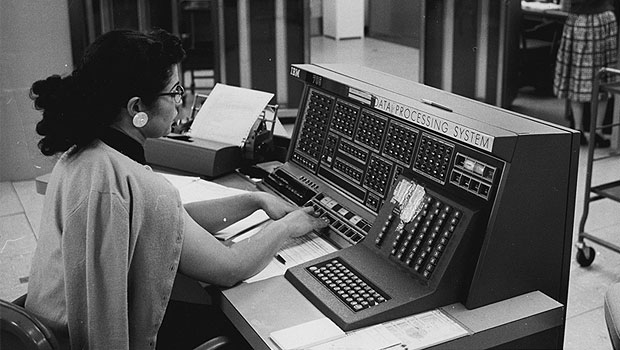
\includegraphics[keepaspectratio]{media/C02_tipos_de_sistemas/consola_ibm_705.jpg}
\caption{Operadora en la consola de un mainframe IBM 705 --- Fuente:
\href{https://www.ibm.com/history/700}{IBM}}\label{fig-consola-ibm-705}
\end{figure}

Estos sistemas se convirtieron en \textbf{sistemas de procesamiento por
lotes} o \textbf{sistemas en \emph{batch}} cuando se comenzó a utilizar
un pequeño programa ---llamado \textbf{monitor del sistema}--- cuya
función era cargar y ejecutar sin interrupción un conjunto ---o lote---
de programas.

Para preparar los lotes, por lo general, el operador cargaba previamente
en cinta magnética el conjunto de programas a partir de las tarjetas
perforadas proporcionadas por los programadores. Como se ilustra en la
\hyperref[fig-sistemas-procesamiento-lotes]{Gestión de trabajos en
sistemas de procesamiento por lotes.}, para ello se utilizaba un
ordenador autónomo ---independiente del \emph{mainframe}--- con lector
de tarjetas y unidad de cinta. Posteriomente, el operador movía la cinta
con el conjunto de programas a la unidad de cinta de entrada del
\emph{mainframe} y lanzaba la ejecución del \textbf{monitor del
sistema}, para que este se encargara de ir leyendo y ejecutando cada uno
de los programas. Para obtener mayor rendimiento, los resultados de los
programas se escribían en una unidad de cinta diferente. Cuando
terminaba la ejecución de todo el conjunto, el operador llevaba la cinta
a otro ordenador autónomo para leer los resultados e imprimrlos, con el
objeto de entregárselos a los programadaores.

\begin{figure}
\centering
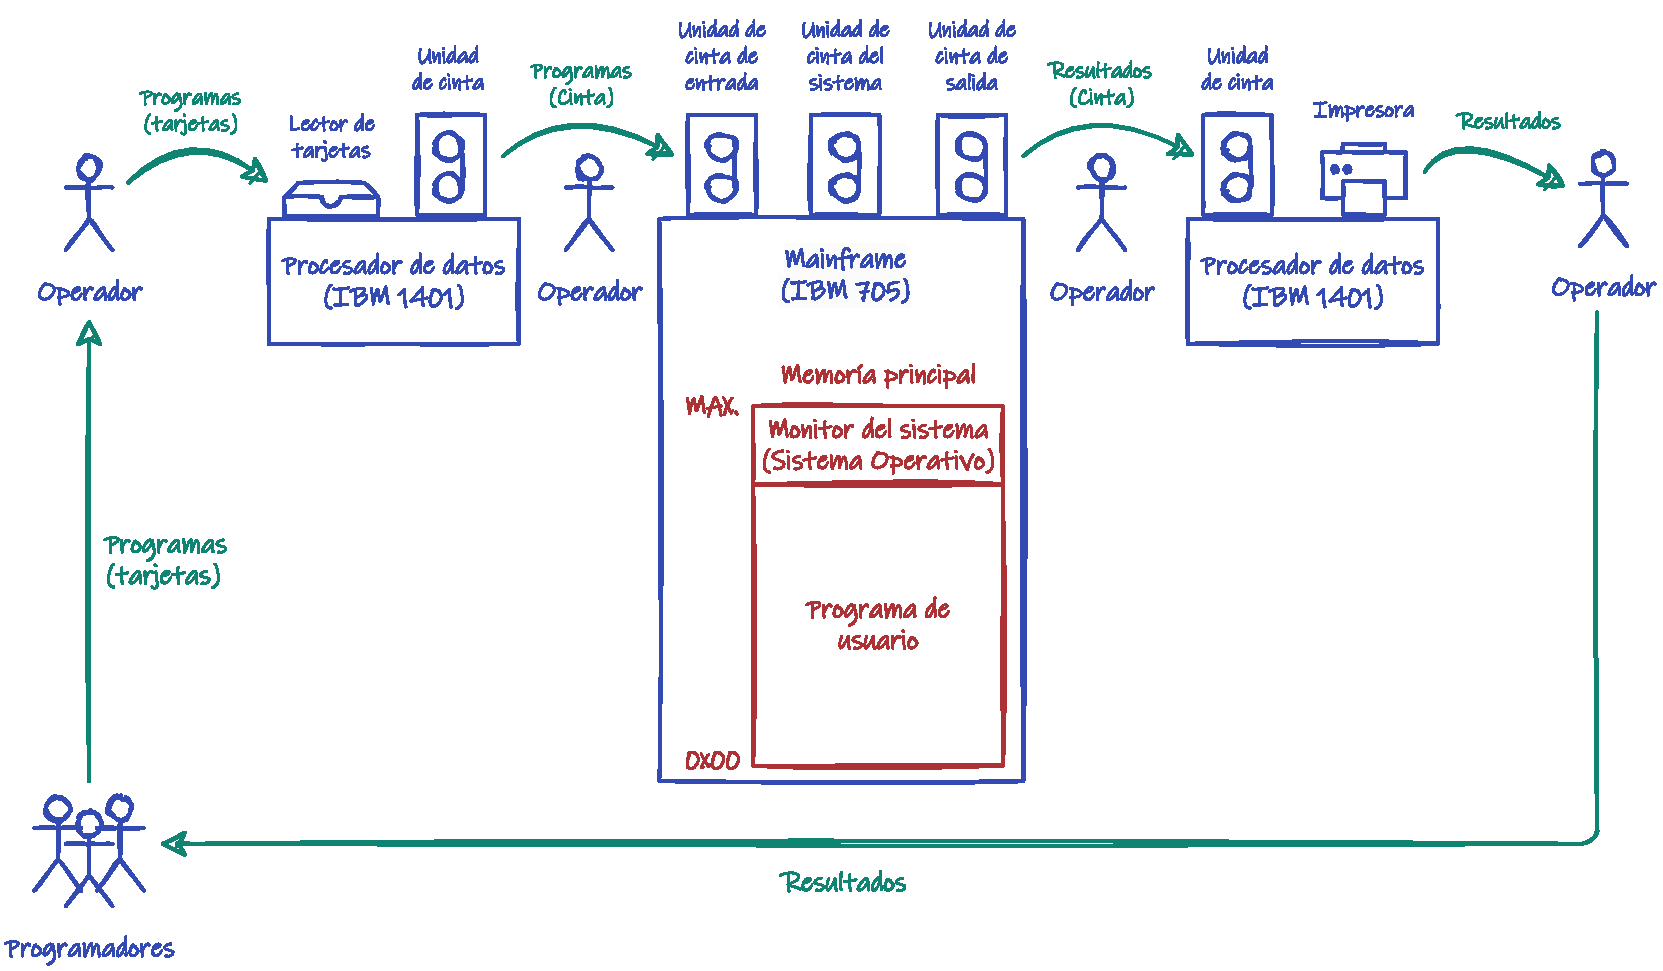
\includegraphics[width=0.8\textwidth]{media/C02_tipos_de_sistemas/sistemas_procesamiento_lotes.pdf}
\caption{Gestión de trabajos en sistemas de procesamiento por
lotes.}\label{fig-sistemas-procesamiento-lotes}
\end{figure}

El \textbf{{}monitor del sistema} es un predecesor de los sistemas
operativos y tenía las siguientes características:

\begin{itemize}
\item
  Permanecía cargado durante todo el tiempo en la memoria del sistema
  (véase la \hyperref[fig-sistemas-procesamiento-lotes]{Gestión de
  trabajos en sistemas de procesamiento por lotes.}).
\item
  Su única tarea era cargar y transferir automáticamente la ejecución de
  un programa al siguiente cuando el anterior terminaba.
\item
  El mayor inconveniente de este tipo de sistemas era que la CPU
  permanecía mucho tiempo desocupada porque era ---y sigue siendo---
  varios órdenes de magnitud más rápida que los dispositivos de E/S.
\end{itemize}

Cualquier programa necesita realizar operaciones de E/S para obtener los
datos requeridos para sus cálculos ---guardados en tarjetas perforadas y
unidades de cinta o, si hablamos de hoy en día, en discos duros y
memorias USB---. También necesita hacer operaciones de E/S para guardar
o imprimir los resultados de esos cálculos.

Si solo se puede ejecutar un programa la vez, cuando el programa
solicita una operación de E/S, la CPU queda a la espera de que esta
termine para continuar con la ejecución del programa, por lo que se
pierde tiempo de CPU en no hacer nada. Este desaprovechamiento de la CPU
es peor cuanto más rápida es la CPU respecto a los dispositivos de E/S.

\subsection{Sistemas multiprogramados}\label{_sistemas_multiprogramados}

{} La solución al inconveniente de los sistemas de procesamiento por
lotes con la E/S fue que los programas no accedieran directamente al
dispositivo de E/S, sino que, en su lugar, solicitaran la operación al
\textbf{monitor del sistema} para que este la solicitara al hardware.
Así el sistema operativo ---como podemos comenzar a llamarlo--- tiene la
oportunidad de sustituir el programa en la CPU por otro, mientras la
operación de E/S se completa.

Además, con la aparición de la tecnología de los discos magnéticos en la
década de los 60 del siglo pasado, los trabajos de los programadores
comenzaron a ser almacenados en discos, desde donde eran escogidos por
el sistema operativo para su ejecución.

A estos sistemas se los llamó \textbf{multiprogramados}, porque
permitían tener varios programas en memoria al mismo tiempo e intercalar
su ejecución en la CPU. A la cantidad de programas cargados en memoria
en un instante dado se la denominaba \textbf{{}grado de
multiprogramación}.

\begin{figure}
\centering
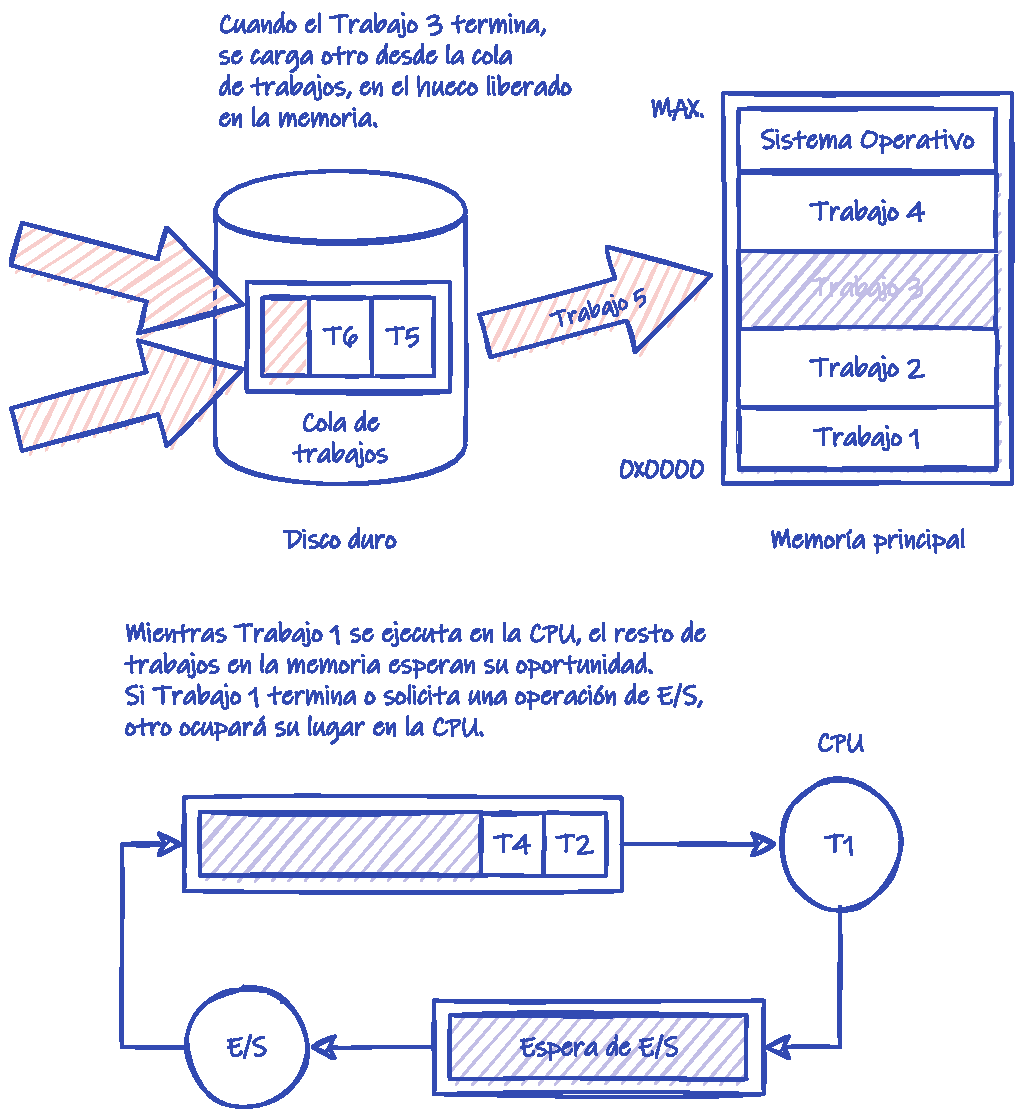
\includegraphics[width=0.8\textwidth]{media/C02_tipos_de_sistemas/sistemas_multiprogramados.pdf}
\caption{Gestión de trabajos en sistemas
multiprogramados.}\label{fig-sistemas-multiprogramados}
\end{figure}

En los \textbf{sistemas multiprogramados} la ejecución de los trabajos
funcionaba de la siguiente manera (véase la
\hyperref[fig-sistemas-multiprogramados]{Gestión de trabajos en sistemas
multiprogramados.}):

\begin{enumerate}
\def\labelenumi{\arabic{enumi}.}
\item
  En el disco magnético se almacenaba una cola donde se iban colocando
  todos los trabajos que tenían que ser ejecutados.
\item
  El sistema operativo cargaba varios trabajos en memoria del conjunto
  de trabajos en la cola en el disco magnético.
\item
  El sistema operativo cede la CPU a uno de los trabajos en memoria.
\item
  Cuando el trabajo en la CPU requería usar la E/S se lo pedía al
  sistema operativo. En lugar de mantener a la CPU ocupada inútilmente,
  el sistema operativo programaba la operación de E/S, pero escogía otro
  trabajo de entre los que estaban en memoria y lo ejecutaba en la CPU.

  Cuando la operación de E/S del anterior trabajo terminaba, el programa
  que ocupaba la CPU no era interrumpido, sino que debía esperar a una
  nueva oportunidad de ser escogido para ejecutarse en la CPU.
\item
  Cuando un programa en la CPU terminaba, sus recursos se liberaban,
  dejando memoria libre. Por lo tanto, el sistema operativo escogía un
  nuevo trabajo de la cola de trabajos en el disco magnético y lo
  cargaba en la memoria.
\end{enumerate}

Todo este proceso se repetía mientras hubiera trabajos que ejecutar en
la cola de trabajos en el disco.

Para operar de la forma descrita es necesario que el sistema operativo
realice tres tareas esenciales:

\begin{itemize}
\item
  La \textbf{planificación de trabajos}, cuya responsabilidad es
  seleccionar el siguiente trabajo que será cargado en la memoria
  principal para mantenerla llena.
\item
  La \textbf{planificación de la CPU}, cuya responsabilidad es elegir el
  siguiente trabajo que será ejecutado en la CPU, de entre los
  disponibles en la memoria principal.
\item
  La \textbf{gestión de la memoria}, cuya responsabilidad es repartir la
  memoria principal entre los trabajos alojados en la misma.
\end{itemize}

Un ejemplo de este tipo de sistemas operativos es el IBM OS/360, que fue
lanzado en 1966 para utilizarlo en los \emph{mainframes} IBM System/360
(véase el \hyperref[sect-historia-segunda-generaciuxf3n]{???}).

\subsection{Sistemas de tiempo
compartido}\label{_sistemas_de_tiempo_compartido}

{} Los sistemas multiprogramados ofrecían un uso más eficiente de la
CPU, pero no eran capaces de proporcionar interacción directa con los
usuarios. Los programadores seguían teniendo que entregar los trabajos
al operador y espera a que este les devolviera los resultados.

Los \textbf{sistemas de tiempo compartido} se desarrollaron tras
observar que al dar acceso a un grupo de usuarios se podía conseguir un
uso más eficiente del sistema, en comparación a cuando solo podía ser
utilizado por un usuario a la vez. Esto es debido a que, generalmente,
un usuario introduce información de forma continua para luego detenerse
durante largos periodos de tiempo, mientras que en un grupo de usuarios,
las pausas de uno de ellos se pueden llenar con la actividad de los
otros.

\begin{figure}
\centering
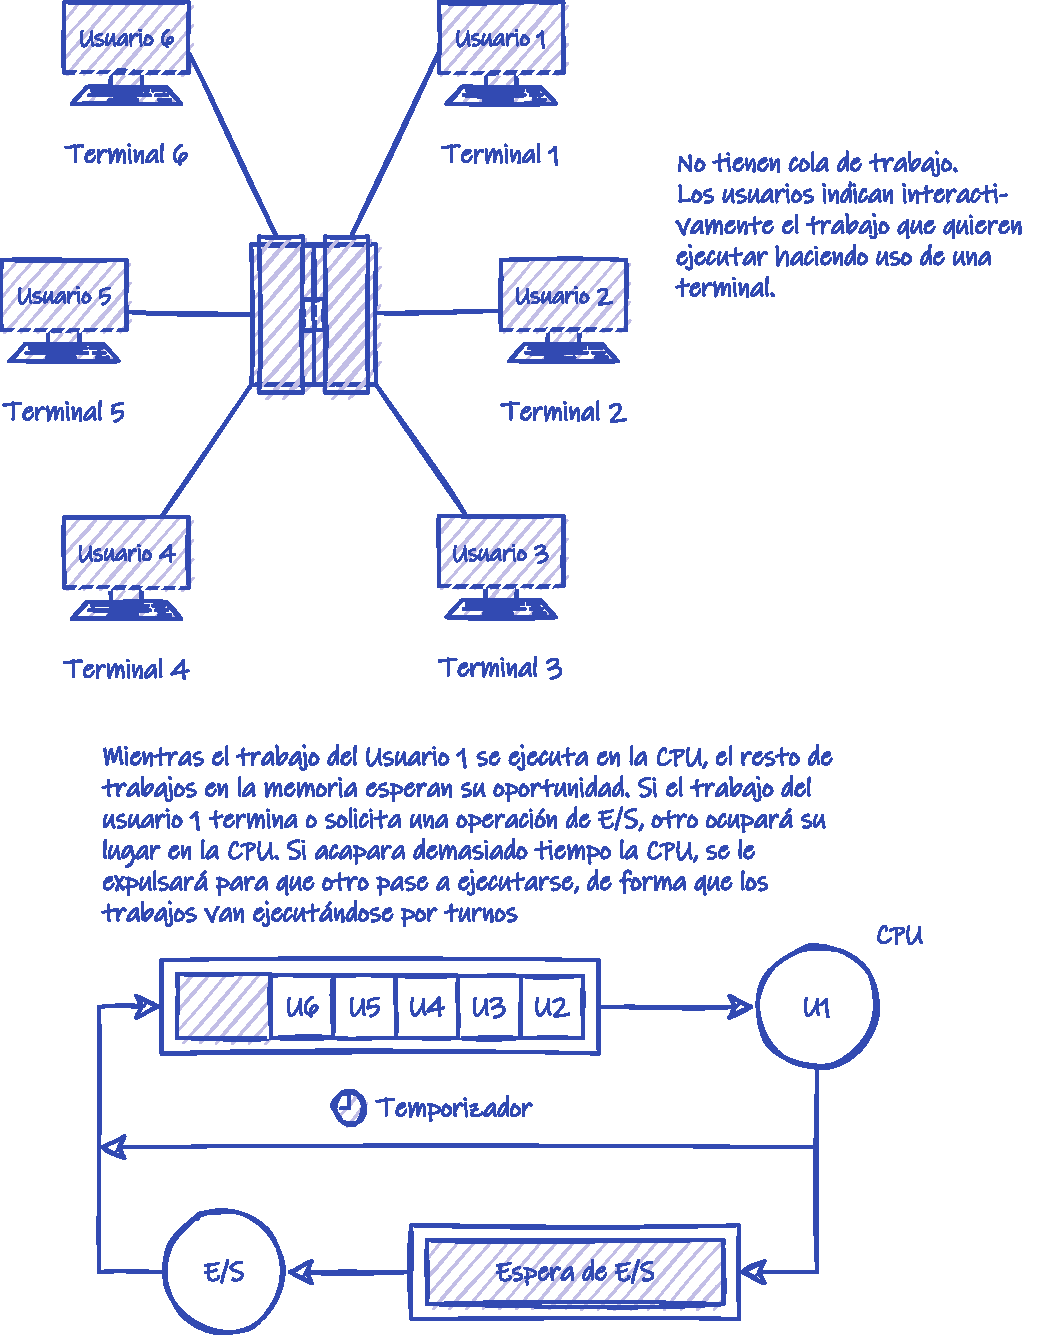
\includegraphics[width=0.8\textwidth]{media/C02_tipos_de_sistemas/sistemas_de_tiempo_compartido.pdf}
\caption{Gestión de trabajos en sistemas de tiempo
compartido.}\label{fig-sistemas-tiempo-compartido}
\end{figure}

Los \textbf{sistemas de tiempo compartido} se caracterizaban por:

\begin{itemize}
\item
  Tener \textbf{terminales}, es decir, hardware especializado en hacer
  de interfaz directa entre los usuarios y el sistema. A través de estas
  terminales los usuarios podían enviar comandos al sistema e
  interactuar con sus trabajos. Podía haber múltiples usuarios al mismo
  tiempo, pero cada uno solo podía tener un trabajo en ejecución a la
  vez.
\item
  Usar la \textbf{multiprogramación} para tener varios trabajos en la
  memoria principal al mismo tiempo e intercambiar el trabajo en la CPU
  cuando este solicitaba una operación de E/S, como ya se venía haciendo
  en los \textbf{sistemas multiprogramados} para hacer un uso más
  eficiente de la CPU.
\item
  Repartir el tiempo de CPU entre usuarios. El sistema operativo
  asignaba un tiempo de CPU a cada usuario ---denominado \textbf{ventana
  de tiempo} o \textbf{{}cuanto} de CPU---. Cuando este tiempo se
  agotaba, el sistema intercambiaba el trabajo en la CPU por el de otro
  usuario en el sistema. La ventana de tiempo era extremadamente
  pequeña, dando a cada usuario la impresión de que su trabajo nunca se
  detenía, como si dispusiera de la CPU en exclusiva.
\end{itemize}

Los sistemas que, como los de tiempo compartido, pueden ser utilizados
por varios usuarios simultáneamente se denominan sistemas
\textbf{{}multiusuario} {}.

En los primeros sistemas se usaban \textbf{{}terminales}
electromecánicos con un teclado y una impresora, como el
\href{https://en.wikipedia.org/wiki/Teletype_Model_33}{Teletype Model 3}
(1963). Posteriormente llegaron los terminales electrónicos, que usaban
un monitor en lugar de una impresora, como el
\href{https://es.wikipedia.org/wiki/IBM_3270}{IBM 3270}. En cualquier
caso solo disponían del hardware necesario para realizar la tarea de
conectar a los usuarios con el ordenador central.

Estos terminales no deben confundirse con las terminales por software
que traen algunos sistemas operativos modernos. Las terminales por
software o \emph{terminales virtuales} se programan para emular las
especificaciones de alguna versión de esas terminales físicas antiguas
que hemos comentado.

Los sistemas de tiempo compartido significaron un salto importante en
complejidad por diversas razones:

\begin{itemize}
\item
  Como varios trabajos están en la memoria principal al mismo tiempo, el
  sistema operativo requiere mecanismos de \textbf{gestión de la
  memoria} y \textbf{protección}.
\item
  Para tener un tiempo de respuesta razonable, los trabajos deben estar
  cargados en la memoria principal. Para que quepan más trabajos de los
  usuarios en la memoria, el sistema operativo debe utilizar técnicas de
  \textbf{memoria virtual} para ejecutar trabajos que no están
  completamente cargados en la memoria principal.
\item
  Como la CPU debe ser compartida entre todos los trabajos, el sistema
  operativo necesita mecanismos de \textbf{planificación de la CPU}.
\item
  Como varios trabajos pueden tener la necesidad de cooperar y que su
  ejecución siga cierto orden, el sistema operativo debe proporcionar
  mecanismos de \textbf{sincronización} y \textbf{comunicación}.
\item
  Como el sistema debe disponer de un \textbf{sistema de archivos} para
  repartir el espacio en disco y facilitar a los usuarios el acceso y
  gestión de sus datos, el sistema operativo necesita un componente de
  \textbf{gestión de discos}.
\end{itemize}

Las primeras versiones de UNIX ---lanzado por primera vez en 1970--- el
sistema operativo VMS ---desarrollado en 1978--- para los VAX de Digital
Equipment Corportation y el IBM OS/400 ---introducido en 1988---
utilizado en los minicomputadoras AS/400, son algunos ejemplos de
sistemas operativos de tiempo compartido (véase el
\hyperref[sect-historia-tercera-generaciuxf3n]{???}).

Estrictamente hablando, el término \textbf{sistemas de tiempo
compartido} hace referencia a estos \emph{mainframes} desarrollados a
partir de principios de la década de 1970. Así que no es común
utilizarlo con \emph{mainframes} modernos.

Los \emph{mainframes} modernos permiten a un mismo usuario ejecutar
varios trabajos al mismo tiempo, repartiendo el tiempo de CPU entre
todos los trabajo en el sistema y no solo entre los usuarios. Y lo mismo
ocurre en la mayor parte de los sistemas operativos de propósito general
actuales ---utilizados en ordenadores de escritorio, servidores,
portátiles y dispositivos móviles--- que con el tiempo han copiado
muchas características de los \textbf{sistemas de tiempo compartido}.
Por eso el término actual es \textbf{sistema multitarea}, que es mucho
más general.

La \textbf{{}multitarea} {} es un método para tener varios procesos en
memoria y ejecutarlos «al mismo tiempo». Generalmente requiere de
técnicas de multiprogramación, como las empleadas por los antiguos
\textbf{sistemas multiprogramados}, y de reparto del tiempo de CPU, como
ocurre en los antiguos \textbf{sistemas de tiempo compartido}. Por eso
se puede decir que ambos tipos de sistemas \emph{mainframe} eran
\textbf{sistemas multitarea}. Al igual que lo son los \emph{mainframes}
modernos y muchos sistemas operativos actuales de escritorio y de
dispositivos móviles.

\section{Sistemas de escritorio}\label{_sistemas_de_escritorio}

{} En la década de los 70 del siglo pasado también aparecieron las
primeras CPU en microprocesadores y con estas llegaron las
\textbf{microcomputadoras} o \textbf{microordenadores}. Las primeras
\textbf{{}microcomputadoras} no incluían teclado ni monitor y se
programaban usando interruptores y ledes ubicados en el frontal de la
unidad. Pero en torno a 1977 apareció la segunda generación de
\textbf{microcomputadoras}, que sí incluían estos periféricos de E/S,
por lo que eran más fáciles de usar que sus predecesoras. Entonces
comenzaron a recibir el nombre de \emph{ordenadores domésticos} y de su
mano llegaron los primeros \textbf{sistemas operativos de escritorio}.

\begin{figure}
\centering
\includegraphics[keepaspectratio]{media/C02_tipos_de_sistemas/ordenadores_domésticos_1977.jpg}
\caption{Los tres ordenadores que la revista Byte denominó como la
"Trinidad de 1977" de la computación doméstica: el
\href{https://es.wikipedia.org/wiki/Commodore_PET}{Commodore PET 2001},
el \href{https://es.wikipedia.org/wiki/Apple_II}{Apple II} y el
\href{https://es.wikipedia.org/wiki/TRS-80}{TRS-80 Model I} --- Fuente:
\href{https://commons.wikimedia.org/wiki/File:Trinity77.jpg}{Wikipedia}}\label{fig-ordenadores-domuxe9sticos-1977}
\end{figure}

Los \emph{mainframes} y las minicomputadoras de la época siguieron
siendo los ordenadores corporativos por excelencia, ya que eran mucho
más grandes y potentes, y también costosos.

El término en desuso \textbf{{}minicomputadora} o
\textbf{{}miniordenador} hace referencia a máquinas multiusuario de
rango medio, entre los \emph{mainframes} y los ordenadores domésticos.

Los primeros \textbf{sistemas operativos de escritorio} eran muy
básicos. Por ejemplo, en un sistema diseñado para ser utilizado por un
único usuario no tiene sentido implementar un sistema de archivos con
permisos. Así que, los primeros sistemas operativos de escritorio
carecían de esta característica que, sin embargo, ya existía en los
sistemas de tiempo compartido de la época. De la misma manera, carecían
de otros mecanismos de protección y no eran ni multiusuario ni
multitarea.

Pese a estas diferencias, los \textbf{sistemas operativos de escritorio}
se han beneficiado del desarrollo de los sistemas operativos para
\emph{mainframes}. Los sistemas de escritorio actuales son
\textbf{multiusuario} y \textbf{multitarea}; incluyen sistemas de
archivos con permisos, autenticación y mecanismos de protección de la
memoria ---como medidas para proteger los datos de los usuarios--- y han
incorporado muchas otras características de los sistemas operativos para
\emph{mainframe}.

Aunque con el tiempo los sistemas de escritorio han ido adquiriendo
características desarrolladas en los \emph{mainframes}, no debemos
olvidar que ambos tipos de sistemas se siguen diseñando con objetivos
diferentes. Mientras que en los \emph{mainframes} se persigue maximizar
la fiabilidad y utilización eficiente de los recursos, en los sistemas
de escritorio se maximiza la facilidad de uso y el tiempo de respuesta
al usuario, poniendo algo de atención al rendimiento.

Los \textbf{sistemas operativos de escritorio} modernos ya nos son «solo
de escritorio» ni se ejecutan únicamente en ordenadores domésticos. Se
utilizan en un altísimo porcentaje en servidores, superordenadores y
hasta en dispositivos móviles. Por eso, en la actualidad, el término
\textbf{sistema operativo de propósito general} {} es mucho más
adecuado.

El \textbf{tiempo de respuesta} al usuario se puede considerar como el
intervalo de tiempo entre un comando de un usuario ---por ejemplo un
clic--- y la respuesta del sistema a dicho comando. En ocasiones este
tiempo se minimiza a costa de un uso menos eficiente de los recursos del
sistema, por lo que no es un objetivo deseable para diseñar un
\emph{mainframe}. Para más información, véase el
\hyperref[_criterios_de_planificaciuxf3n]{???}.

Son muchos los ejemplos de sistemas operativos en esta categoría. Van
desde CP/M ---lanzado en 1977--- hasta los actuales GNU/Linux, Microsoft
Windows y Apple macOS, pasando por MS-DOS, IBM OS/2 y todas las
versiones anteriores de Microsoft Windows (véase el
\hyperref[sect-historia-cuarta-generaciuxf3n]{???}).

\section{Sistemas de mano}\label{_sistemas_de_mano}

{} {} Con el nombre genérico de \textbf{sistemas de mano} ---del inglés
\emph{handheld}--- hacemos referencia a las \emph{tablets},
\emph{smartphones}, lectores de libros electrónicos y otro sistemas
móviles y portátiles. Los desarrolladores de aplicaciones y sistemas de
mano deben enfrentarse a diversos desafíos, originados por el tamaño
limitado de los dispositivos y la alimentación mediante el uso de
baterías. Debido a esas limitaciones, muchos sistemas de mano tienen
poca cantidad de memoria, procesadores lentos ---en comparación con sus
equivalentes de escritorio--- y pantallas más pequeñas.

En el diseño del sistema operativo suele primar la facilidad de uso y
buscar un buen equilibrio entre rendimiento y tiempo de vida de la
batería.

\section{Sistemas multiprocesador}\label{_sistemas_multiprocesador}

{} Un \textbf{sistema multiprocesador} es aquel ordenador hay
procesadores interconectados que comparten el bus del sistema, el reloj
y, en ocasiones la memoria, y los periféricos.

Hace años esto solo se daba en sistemas con varias CPU, lo que era
relativamente común en servidores y sistemas de alto rendimiento para
trabajos técnicos o científicos. Sin embargo, en la actualidad cualquier
dispositivo digital u ordenador doméstico puede tener una CPU con
múltiples núcleos, lo que los convierte en sistemas multiprocesador.

Las principales ventajas de estos sistemas son:

\begin{itemize}
\item
  \textbf{Aumentan la cantidad de trabajo realizado}. A mayor número de
  procesadores, mayor cantidad de trabajo puede realizar el sistema. Sin
  embargo debemos de tener en cuenta que un sistema con \emph{N} CPU no
  es un sistema \emph{N} veces más rápido. Cuando varios procesadores
  cooperan para realizar una tarea, existe cierta pérdida de rendimiento
  debida a los mecanismos de sincronización requeridos para controlar el
  acceso a los recursos compartidos por los procesadores.
\item
  \textbf{Economía de escala}. Un sistema multiprocesador puede costar
  menos que múltiples sistemas monoprocesadores conectados para hacer un
  trabajo equivalente, porque comparten periféricos, almacenamiento,
  alimentación, etc.
\item
  \textbf{Alta disponibilidad}. Con el hardware adecuado el sistema
  puede ser tolerante al fallo de uno de los procesadores. En caso de
  fallo el sistema no se detendría, pero sí trabajaría más despacio.
\end{itemize}

En la actualidad existen dos tipos de sistemas multiprocesador:

\begin{figure}
\centering
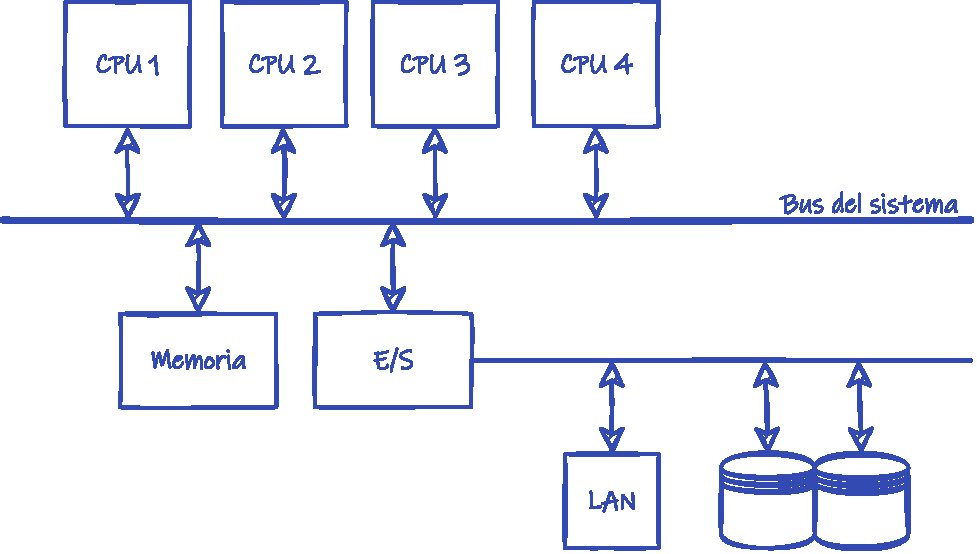
\includegraphics[width=0.8\textwidth]{media/C02_tipos_de_sistemas/multiprocesamiento_simétrico.pdf}
\caption{Arquitectura de un sistema de multiprocesamiento
simétrico.}\label{fig-smp}
\end{figure}

\begin{itemize}
\item
  En los \textbf{sistemas de multiprocesamiento simétrico}{}{} o
  \textbf{SMP} (\emph{Symmetric Multiprocessing}) todos los procesadores
  son iguales. Todos comparten los mismos recursos, pueden acceder a los
  mismos dispositivos (véase la \hyperref[fig-smp]{Arquitectura de un
  sistema de multiprocesamiento simétrico.}) y cada uno ejecuta una
  copia del núcleo del sistema operativo. El sistema operativo debe
  haber sido diseñado para saber repartir el trabajo entre los
  procesadores y compartir adecuadamente entre tareas y procesadores el
  resto de recursos del sistema. Casi todos los sistemas multiprocesador
  modernos son de este tipo.
\item
  En los \textbf{sistemas de multiprocesamiento asimétrico}{}{} o
  \textbf{AMP} (\emph{Asymmetric Multiprocessing}) hay un procesador
  principal y varios secundarios a quienes el principal planifica y
  entrega las tareas que deben ejecutar. En ocasiones los procesadores
  secundarios se distinguen del principal por haber sido diseñados para
  realizar algún tipo concreto de tareas de forma muy eficiente o por
  estar conectadas a hardware especial. Ejemplos de esto son las
  \href{https://es.wikipedia.org/wiki/Unidad_de_procesamiento_gr\%C3\%A1fico}{GPU},
  que no son sino procesadores diseñados específicamente para el
  procesamiento de gráficos, o las CPU de E/S conectadas a discos duros
  para gestionarlos de forma más eficiente.
\end{itemize}

Un ejemplo bastante ilustrativo es el de
\href{https://es.wikipedia.org/wiki/Cell_(microprocesador)}{Cell}, la
CPU de PlayStation 3. Tenía un núcleo principal de propósito general y 8
núcleos optimizados para ejecutar, de forma muy eficiente, operaciones
vectoriales. Con la ayuda del sistema operativo, los programas debían
envíar tareas matemáticamente intensivas a los procesadores secundarios,
si querían extraer el máximo provecho de la arquitectura.

Desarrollar para un sistema así es más complejo. Por lo que, aunque
sobre el papel esta arquitectura ofrecía gran rendimiento, aprovecharlo
era un verdadero reto para los desarrolladores.

\section{Sistemas distribuidos}\label{_sistemas_distribuidos}

{} En la actualidad es común el uso de redes para interconectar
ordenadores individuales ---por ejemplo Internet o la red de área local
de una oficina--- cada uno equipado con su procesador, su memoria, sus
dispositivos de almacenamiento, su fuente de alimentación, etc. En las
redes de ordenadores los procesadores de dichos ordenadores se comunican
con otros procesadores a través de líneas de comunicación, como: redes
Ethernet, líneas telefónicas o wifi. Estos sistemas son comúnmente
denominados \textbf{sistemas distribuidos}.

Sin entrar en detalles, los sistemas distribuidos pueden ser
clasificados en \textbf{sistemas cliente-servidor} y \textbf{sistemas de
redes entre iguales}.

\subsection{Sistemas cliente-servidor}\label{_sistemas_cliente_servidor}

En los \textbf{sistemas {}cliente-servidor} {} existen ordenadores que
actúan como \textbf{servidores} encargados de satisfacer las peticiones
generadas por otros ordenadores que actúan como \textbf{clientes}.

Este tipo de sistemas han sustituido, en un gran número de casos, a los
terminales conectados a \emph{mainframes}, debido a que los sistemas de
escritorio son cada vez más potentes y baratos. Concretamente:

\begin{itemize}
\item
  Los terminales han sido sustituidos por sistemas de escritorio que, al
  disponer de más recursos, son capaces de realizar muchas de las
  funcionalidades que anteriormente eran manejadas directamente por los
  \emph{mainframes}.
\item
  Al mismo tiempo estos \emph{mainframes} se han reemplazado por
  servidores, no muy diferentes a los sistemas de escritorios, pero
  preparados para atender las peticiones de sus clientes.
\end{itemize}

Ejemplos de este tipo de sistemas son los servidores de base de datos,
que responden a las consultas SQL de los clientes, o los servidores de
archivos, que proporcionan una interfaz de sistema de archivos con la
que los clientes pueden crear, leer, escribir y borrar archivos en el
servidor; de forma similar a como si estuvieran almacenados localmente
en el propio cliente.

\subsection{Sistemas de redes entre
iguales}\label{_sistemas_de_redes_entre_iguales}

En los \textbf{sistemas de redes entre iguales} {} {} o \textbf{{}P2P}
(\emph{peer-to-peer}) clientes y servidores no se distinguen los unos de
los otros. Todos los nodos del sistema son iguales y cada uno puede
actuar como cliente o servidor, dependiendo de cuándo piden o
proporcionan un servicio.

La ventaja fundamental de este tipo de sistemas es que en los sistemas
cliente-servidor el servidor puede ser el cuello de botella del
rendimiento, pero en los sistemas de redes entre iguales la carga se
distribuye entre todos los nodos de la red. Ejemplos de este tipo de
sistemas son las redes
\href{https://es.wikipedia.org/wiki/BitTorrent}{BitTorrent} y
\href{https://es.wikipedia.org/wiki/Bitcoin}{Bitcoin}.

Un servidor puede ser el cuello de botella no solo por su potencia sino
también por el ancho de banda de su conexión a la red. La potencia del
servidor es lo de menos cuando se intenta distribuir en Internet
archivos de gran tamaño ---por ejemplo imágenes de CD o DVD--- pues el
problema es que varias descargas simultáneas pueden consumir todo el
ancho de banda del servidor durante largos periodos de tiempo.

\subsection{Sistemas operativos para sistemas
distribuidos}\label{_sistemas_operativos_para_sistemas_distribuidos}

Desde el punto de vista de los sistemas operativos para sistemas
distribuidos es posible hacer la siguiente distinción:

\begin{itemize}
\item
  Los \textbf{sistemas operativos de red} {} ofrecen a las aplicaciones
  que corren sobre ellos servicios de acceso a redes de ordenadores. Por
  ejemplo, implementan algún mecanismo que permita a diferentes procesos
  en diferentes ordenadores enviar y recibir mensajes. Además suelen
  incorporar la opción de proporcionar algunos servicios de red, como la
  compartición de archivos y dispositivos con otros equipos de la misma
  red.

  Los ordenadores con sistemas operativos de red son autónomos.
  Simplemente es que gracias al sistema operativo de red, conocen la
  existencia de la red y saben usarla para comunicarse con otros
  ordenadores de la misma.

  Este tipo de sistemas operativos son los más utilizados en los tipos
  de sistemas distribuidos comentados anteriormente. En la actualidad,
  la inmensa mayoría de sistemas de escritorio y dispositivos de mano
  utilizan sistemas operativos de red.
\item
  Los \textbf{sistemas operativos distribuidos} {} crean en el usuario
  la ilusión de que está en un único ordenador, aunque en realidad el
  sistema operativo controla todos los ordenadores de la red, dando al
  usuario acceso transparente a los recursos en todos los equipos de la
  misma.

  Con este tipo de sistemas operativos el usuario no sabe en qué
  ordenador se ejecutan sus procesos, donde se almacenan sus archivos,
  ni qué equipo tiene conectado los distintos periféricos a los que
  tiene acceso.
\end{itemize}

Un ejemplo de sistema operativo distribuido es
\href{https://en.wikipedia.org/wiki/Amoeba_(operating_system)}{Amoeba},
un sistema operativo distribuido de investigación escrito por Andrew S.
Tanenbaum en Vrije Universiteit. Para más información, véase el
\href{http://www.cs.vu.nl/pub/amoeba/}{sitio web de Amoeba}.

\section{Sistemas en clúster}\label{_sistemas_en_cluxfaster}

{} Como los sistemas distribuidos, los \textbf{sistemas en clúster}
interconectar ordenadores individuales. Sin embargo, generalmente se
acepta que los \textbf{sistemas en clúster} comparten el almacenamiento
y estén conectados por medio de una red local, condiciones que no tienen
por qué darse en los sistemas distribuidos.

Los \textbf{sistemas en clúster} se utilizan para:

\begin{itemize}
\item
  \textbf{Obtener servicios con alta disponibilidad}. Para ello un nodo
  del clúster puede estar ejecutando un servicio mientras otro nodo lo
  monitoriza. En caso de fallo en el nodo que da el servicio, el que lo
  monitoriza lo sustituye.

  Si es necesario proporcionar varios servicios, el mecanismo anterior
  se puede extender repartiendo los servicios entre dos o más nodos y
  haciendo que se monitoricen entre ellos.
\item
  \textbf{Computación de alto rendimiento} o \textbf{HPC}. En este caso
  todos los nodos se utilizan para dar un mismo servicio. Un nodo
  especial, denominado balanceador de carga, tiene la responsabilidad de
  repartir el trabajo entre los nodos.

  Este tipo de \textbf{sistemas en clúster} se utiliza para realizar
  trabajos de cálculo muy pesados, como simulaciones ---por ejemplo
  simulación meteorológica, nuclear o de gestión hospitalaria--- o
  romper sistemas de cifrado.
\end{itemize}

También es muy utilizado en servidores de Internet ---como servidores
web, correo electrónico o de mensajería instantánea--- o servidores de
base de datos que deben dar servicio a una gran cantidad de clientes
simultáneamente. En estos casos el balanceador de carga realiza su
trabajo repartiendo las conexiones de los usuarios entre los servidores
del clúster.

\section{Sistemas de tiempo real}\label{_sistemas_de_tiempo_real}

{} Los \textbf{sistemas de {}tiempo real} se utilizan cuando existen
requerimientos estrictos de tiempo en la ejecución de ciertas tareas o
en el procesamiento de flujos de datos.

En general se usan frecuentemente en dispositivos de control donde,
dentro de unos márgenes estrictos de tiempo, se deben tomar datos de uno
o varios sensores, para analizarlos posteriormente y realizar, en
consecuencia, alguna acción con algún mecanismo de control. Por ejemplo,
se suelen utilizar en sistemas de control industrial, domótica,
armamento, automoción ---en la inyección electrónica de combustible,
sistemas de frenado y de control de tracción--- o en dispositivos
médicos.

Los \textbf{sistemas de tiempo real} están muy relacionados con los
\textbf{sistemas empotrados}{}. Estos últimos:

\begin{itemize}
\item
  Se diseñan para realizar tareas muy específicas. No son sistemas de
  propósito general sino de propósito específico.
\item
  Sus sistemas operativos tienen características muy limitadas y no
  tienen que tener necesariamente una interfaz de usuario.
\item
  Estos sistemas están tanto en el motor de los automóviles y los robots
  que los fabrican, como en reproductores de DVD, microondas o
  dispositivos de red.
\end{itemize}

Los \textbf{sistemas de tiempo real} pueden ser clasificados en
\textbf{sistemas de tiempo real estricto} y \textbf{sistemas de tiempo
real flexible}:

\begin{itemize}
\item
  Los \textbf{sistemas de tiempo real estricto} {}{} o \textbf{{}hard
  real-time} garantizan que las tareas serán realizadas dentro de unos
  márgenes estrictos de tiempo.

  Para ello, todas las situaciones imprevistas que puedan ocasionar
  retrasos en el funcionamiento del sistema operativo deben estar
  perfectamente delimitadas en tiempo. Por lo tanto, suelen carecer de
  memoria virtual y de otras abstracciones que aíslen al desarrollador
  del funcionamiento real del hardware, ya que introducen
  impredecibilidad.

  Los sistemas de tiempo real estricto no son compatibles con los
  sistemas de tiempo compartido.
\item
  Los \textbf{sistemas de tiempo real flexible} {} {} o \textbf{{}soft
  real-time} son útiles cuando en un sistema operativo convencional hay
  tareas que tienen mayor importancia que el resto, por lo que deben ser
  realizadas con mayor prioridad.

  El tiempo real flexible no sirve cuando se tienen tareas con
  limitaciones precisas de tiempo, porque no hay manera de garantizar
  que dichas restricciones se van a cumplir. Sin embargo sí es útil para
  tareas relacionadas con la multimedia, la realidad virtual, los
  videojuegos, etc. y es compatible con la memoria virtual y otras
  características presentes en los sistemas de escritorio. Por eso la
  mayor parte de los sistemas de escritorio actuales soportan tareas de
  tiempo real flexible.
\end{itemize}

\section{}

\textbf{Tiempo de lectura:} \{s03-reading-time\}

La historia de los sistemas operativos se puede dividir en cinco grandes
etapas o generaciones, obviamente conectadas con las generaciones de los
ordenadores donde funcionaban.

\section{1ª Generación
(1945-55)}\label{sect-historia-primera-generaciuxf3n}

En la primera generación de ordenadores no se utilizaban sistemas
operativos.

Sus principales características son:

\begin{itemize}
\item
  Computadoras construidas con electrónica de
  \href{https://es.wikipedia.org/wiki/V\%C3\%A1lvula_termoi\%C3\%B3nica}{válvulas
  de vacío}.
\item
  Sin sistema operativo.
\item
  Sin lenguajes de programación. Se programaban directamente en lenguaje
  máquina.
\end{itemize}

Algunos ejemplos de ordenadores destacables fueron:

\begin{description}
\item[\href{https://es.wikipedia.org/wiki/ENIAC}{ENIAC} (1945)]
Se le considera el primer ordenador electrónico digital de propósito
general, aunque existe cierta polémica sobre este punto. Lo cierto es
que se construyeron otros ordenadores antes que este, pero o no eran de
propósito general ---como las famosas computadoras
\href{https://es.wikipedia.org/wiki/Colossus}{Colossus} (1944), que
fueron diseñadas para ayudar en
\href{https://es.wikipedia.org/wiki/Criptoan\%C3\%A1lisis}{criptoanálisis}---
o no eran electrónicos sino electromecánicos ---como la computadora
\href{https://es.wikipedia.org/wiki/Z3}{Z3} (1941), que usaba
\href{https://es.wikipedia.org/wiki/Rel\%C3\%A9}{relés}---.

No era un producto comercial sino un proyecto experimental de defensa
que principalmente se diseñó y utilizó para calcular tablas de tiro de
artillería destinadas al Laboratorio de Investigación Balística del
Ejército de los Estados Unidos.

\href{https://es.wikipedia.org/wiki/Z4}{Z4} (1945) fue el primer
ordenador digital comercial, pero era electro-mecánico.
\item[\href{https://es.wikipedia.org/wiki/IBM_701}{IBM 701} (1953)]
Fue el primer \emph{mainframe} de la serie IBM 700, que a la larga se
convertiría en un éxito de ventas. Utilizaba tubos de vacío y tarjetas
perforadas.
\end{description}

El IBM 7090 ---versión transistorizada del 709, que utilizaba válvulas
de vacío, como todos los de la serie 700--- y el posterior 7094, fueron
usados por la NASA para los cálculos de control de las misiones de los
programas espaciales Mercury y Gemini y durante la primera etapa del
programa Apolo.

\section{2ª Generación
(1955-64)}\label{sect-historia-segunda-generaciuxf3n}

En la segunda generación de ordenadores los transistores reemplazaron a
las válvulas de vacío.

En lo que respecta a los sistemas operativos:

\begin{itemize}
\item
  Aparecen los monitores del sistema, que se pueden considerar un
  predecesor de los sistemas operativos.
\item
  Sistema de procesamiento por lotes.
\item
  Se comienzan a utilizar lenguajes de programación, como: ensamblador,
  FORTRAN y COBOL.
\end{itemize}

\href{https://es.wikipedia.org/wiki/GM-NAA_I/O}{GM-NAA I/O}
(\emph{General Motors and North American Aviation Input/Output system})
fue el primer sistema operativo. Fue desarrollado por General Motors
Research Laboratory en 1956 para el \emph{mainframe}
\href{https://en.wikipedia.org/wiki/IBM_704}{IBM 704} con el fin de
automatizar la carga y ejecución de un nuevo trabajo una vez había
terminado el anterior. Para su desarrollo se basaron en un monitor del
sistema creado en 1955 por programadores de General Motors para el IBM
701.

\begin{figure}
\centering
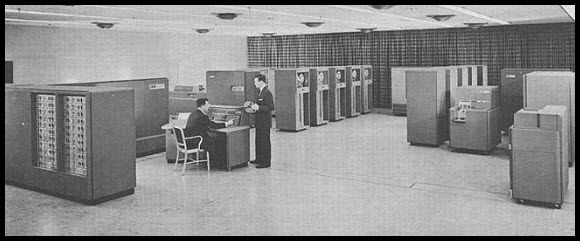
\includegraphics[keepaspectratio]{media/C03_historia/instalación_ibm_702.jpg}
\caption{Instalación de un mainframe IBM 702 --- Fuente:
\href{https://commons.wikimedia.org/wiki/File:BRL61-IBM_702.jpg}{Wikipedia}}\label{fig-instalaciuxf3n-ibm-702}
\end{figure}

\section{3ª Generación
(1965-1968)}\label{sect-historia-tercera-generaciuxf3n}

En la tercera generación se comenzaron a utilizar los circuitos
integrados, que fue una invención de finales de la década de 1950.

En lo que respecta a los sistemas operativos:

\begin{itemize}
\item
  Aparecen los sistemas operativos multiprogramados.
\item
  Aparecen más lenguajes de programación.
\end{itemize}

El ejemplo más destacado de esta época es el \{ibmos360\} Fue un sistema
operativo desarrollado por IBM para su \emph{mainframe}
\href{https://en.wikipedia.org/wiki/IBM_System/360}{IBM System/360}
(S/360) (véase la
\hyperref[fig-instalaciuxf3n-ibm-system-360]{Instalación de un mainframe
IBM System/360 --- Fuente: }). Su versión DOS/360 (\emph{Disk Operating
System/360}) fue el primer sistema operativo en hacer los discos
magnéticos un requisito para poder operar.

\begin{figure}
\centering
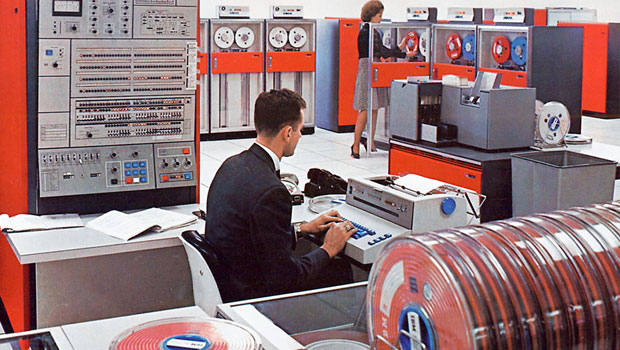
\includegraphics[keepaspectratio]{media/C03_historia/instalación_ibm_system_360.jpg}
\caption{Instalación de un mainframe IBM System/360 --- Fuente:
\href{https://www.ibm.com/history/system-360}{IBM}}\label{fig-instalaciuxf3n-ibm-system-360}
\end{figure}

Se anunció en 1964, pero fue lanzado en 1966, con un año de retraso
respecto a la fecha prevista originalmente. Los motivos fundamentales
fueron ciertos problemas de organización interna de la compañía y la
falta de experiencia en proyectos de esa envergadura. Las previsiones
iniciales eran de 1 millón de líneas de código y miles de componentes de
software.

Algunos autores fechan los inicios de la ingeniería del software en la
publicación del libro «The Mythical Man-Month: Essays on Software
Engineering», escrito por Frederick Brooks y publicado en 1975.
Frederick Brooks se basó en la experiencia adquirida mientras
administraba el desarrollo del IBM OS/360, donde era jefe de proyecto.

\section{4ª Generación
(1965-1980)}\label{sect-historia-cuarta-generaciuxf3n}

La cuarta generación abarca desde mediados de los años 60 hasta finales
de la década de los 70. Respecto a los ordenadores, es el resultado del
desarrollo de los microprocesadores.

En lo que respecta a los sistemas operativos:

\begin{itemize}
\item
  Aparecen los sistemas operativos de tiempo compartido.
\item
  Aparecen los terminales, los programas interactivos y las máquinas
  virtuales.
\end{itemize}

A continuación veremos los ejemplos más representativos de esta época.

\subsection{MULTICS}\label{_multics}

\href{https://es.wikipedia.org/wiki/Multics}{MULTICS} fue anunciado en
1964, fruto de la colaboración entre el MIT, General Electrics y Bell
Labs, como el primer sistema operativo de propósito general.

\begin{figure}
\centering
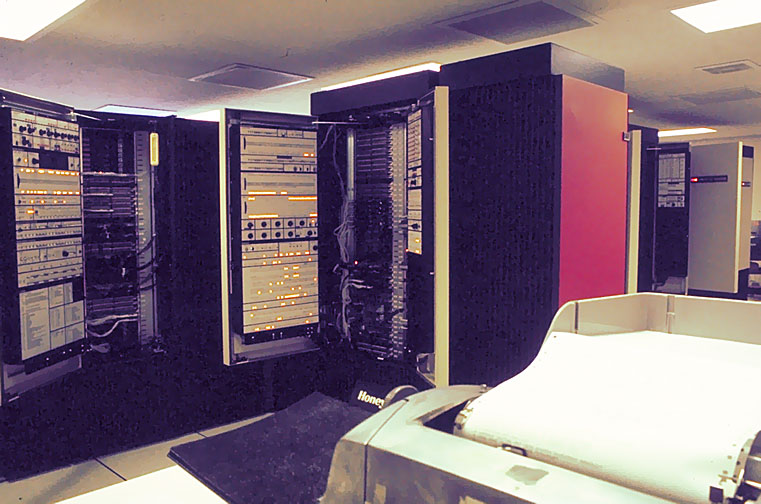
\includegraphics[keepaspectratio]{media/C03_historia/multics_mainframe.jpg}
\caption{Mainframe GE-6180 con sistema MULTICS, en torno a 1976 en el
MIT --- Fuente:
\href{http://www.multicians.org/multics-stories.html}{Multicians}}\label{sect-multics-mainframe}
\end{figure}

Fue el primer sistema operativo en proporcionar un sistema de archivos
jerárquico, intérprete de comandos implementado como programa de
usuario, listas de control de acceso individuales para cada archivo y
enlazado dinámico, entre otras características novedosas.

Además experimentó con eliminar la separación entre el espacio de
direcciones de los procesos y los archivos. Es decir, como si los
archivos estuvieran mapeados en memoria, permitiendo a los procesos
acceder al contenido de los archivos directamente, sin tener que ordenar
manualmente operaciones de lectura desde el disco a la memoria (véase el
\hyperref[_archivos_mapeados_en_memoria]{???}).

\subsection{VM/CMS}\label{_vmcms}

\href{https://es.wikipedia.org/wiki/VM_(sistema_operativo)}{VM/CMS} es
un sistema de IBM utilizado en los \emph{mainframes}
\href{https://en.wikipedia.org/wiki/IBM_System/360}{IBM System/360},
System/370, System/390 y zSeries. VM es un
\href{https://es.wikipedia.org/wiki/Hipervisor}{hipervisor} que se
encarga de virtualizar el hardware para crear múltiples máquinas
virtuales, dando la sensación de que cada una es un \emph{mainframe}
independiente.

Como sistema operativo de las máquinas virtuales, una opción común es
CMS, un sistema interactivo y monousuario muy ligero, diseñado para
operar fundamentalmente en una máquina virtual de VM. Gracias a VM/CMS,
cada usuario tiene la sensación de trabajar en un sistema completamente
independiente y seguro.

El desarrollo de VM/CMS comenzó en 1965 y la primera versión estuvo
disponible a primeros de 1966. Las versiones actuales se denominan IBM
z/VM.

\subsection{UNIX}\label{_unix}

\{unix\} fue desarrollado originalmente por Bell Labs en 1970 para los
sistemas \href{https://es.wikipedia.org/wiki/PDP-11}{PDP-11/20} (véase
la \hyperref[fig-dec-pdp11]{Dennis Ritchie (de pie) y Ken Thompson
(sentado) frente a un PDP-11 y sus dos terminales  --- Fuente: }). La
autoría de este se le atribuye a un grupo de programadores, liderados
por Ken Thompson, que decidieron rehacer el trabajo de MULTICS, pero a
menor escala, después de que Bell Labs abandonara el proyecto MULTICS en
1969. Inicialmente se llamó UNICS y fue desarrollado para los sistemas
PDP-7 ---una minicomputadora de la serie PDP de Digital Equipment
Corporation (DEC)---.

\begin{figure}
\centering
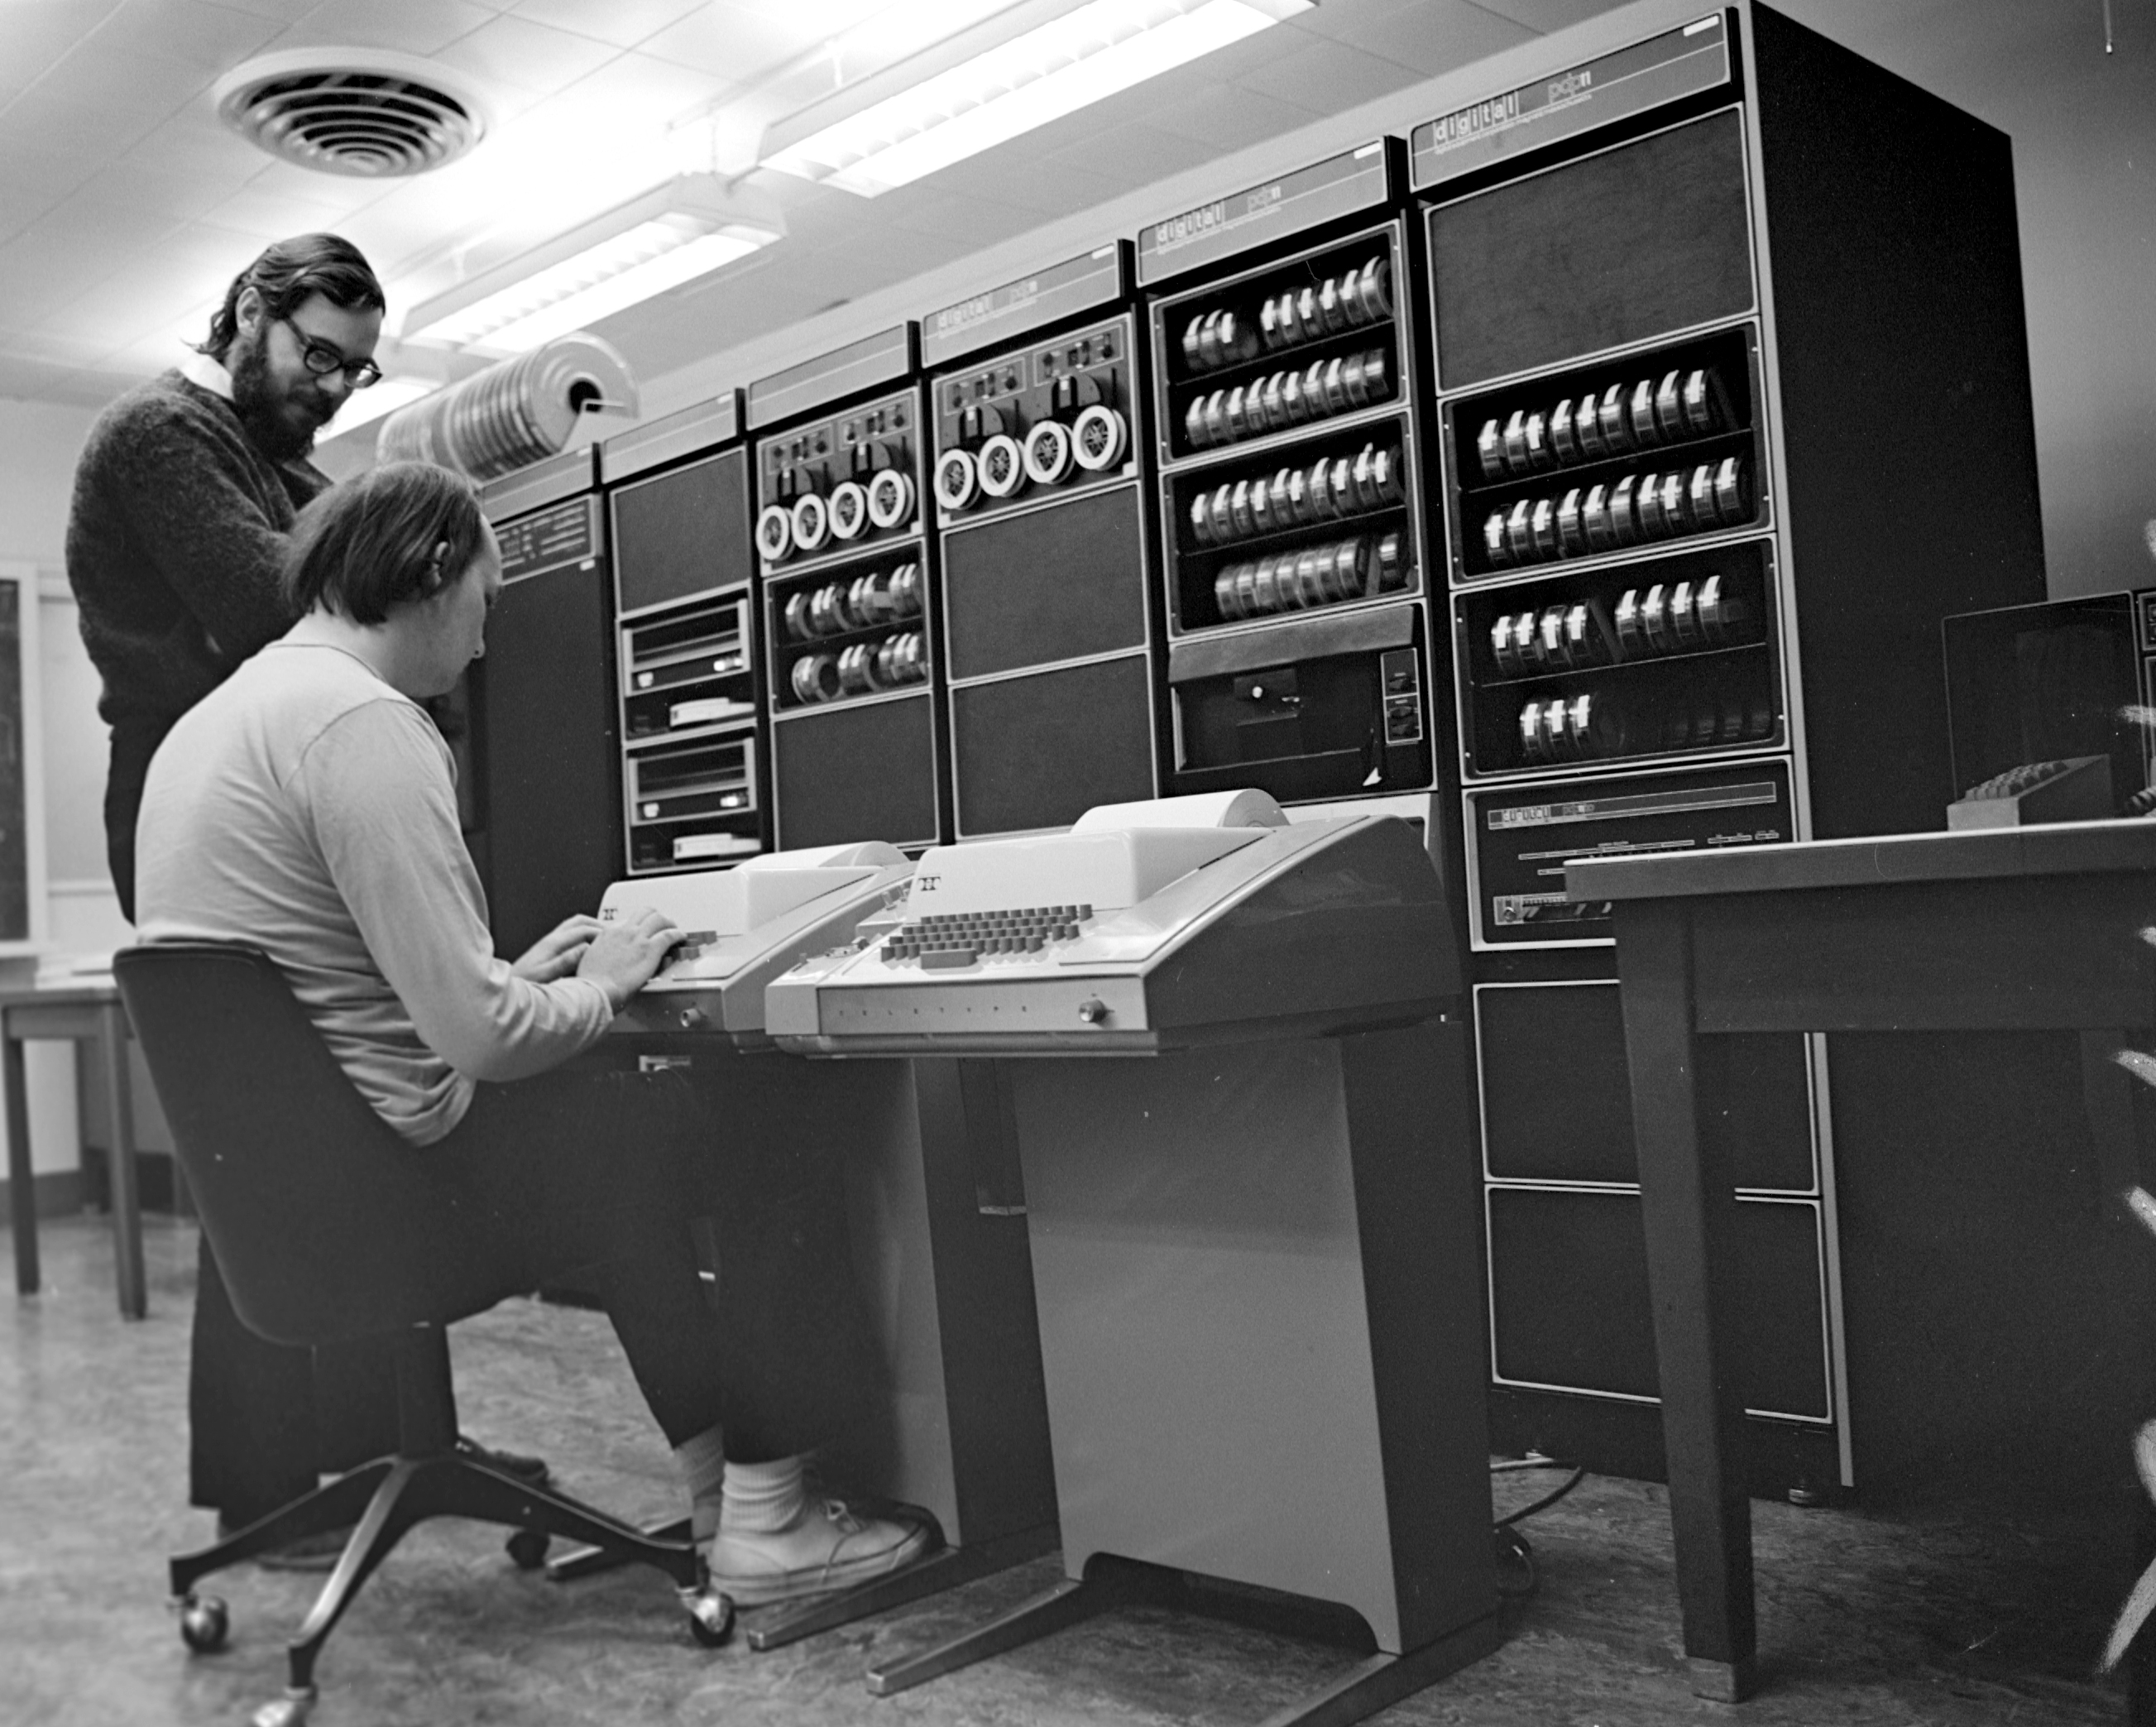
\includegraphics[keepaspectratio]{media/C03_historia/dec_pdp11_ken_den.jpg}
\caption{Dennis Ritchie (de pie) y Ken Thompson (sentado) frente a un
PDP-11 y sus dos terminales
\href{https://en.wikipedia.org/wiki/Teletype_Model_33}{Teletype
33} --- Fuente: \href{https://www.bell-labs.com/usr/dmr/www/}{Dennis
Ritchie}}\label{fig-dec-pdp11}
\end{figure}

Los sistemas UNIX se caracterizan por ofrecer un gran número de pequeñas
herramientas especializadas diseñadas para trabajar unidas ---a través
de la línea de comandos usando tuberías--- y por usar la E/S salida de
archivos como modelo universal de E/S. Es decir, que los dispositivos,
ciertos mecanismos de comunicación entre procesos y hasta algunos
aspectos de la configuración e información del sistema son gestionados
como archivos.

La primera versión de UNIX fue implementada en ensamblador, como era
común en la época. Posteriormente, Dennis Ritchie y Brian Kernighan
diseñaron un nuevo lenguaje de programación llamado «C», especialmente
pensado para que UNIX fuera escrito con él. Eso facilitó que UNIX
pudiera ser portado a ordenadores diferentes. Además, gracias al
lenguaje C, el código era más conciso y compacto, lo que se tradujo en
que se pudieron desarrollar nuevas funcionalidades más rápidamente.

AT\&T, la compañía matriz de Bell Labs, no podía competir en la
industria de los ordenadores, por lo que puso el código fuente de UNIX a
disposición de universidades, compañías privadas y del gobierno de los
Estados Unidos. Eso aumentó su difusión y dio resultados inesperados.
Por ejemplo, una de las variantes más importantes de UNIX fue \{bsd\},
desarrollada por la Universidad de California en Berkeley.

La versión 4.2BSD (\emph{Berkeley Software Distribution}) de esta
variante de UNIX fue la primera que incluyó la interfaz de
\emph{sockets} para facilitar la comunicación entre procesos a través de
Internet y otras redes. Esta interfaz se ha convertido en estándar en
prácticamente cualquier sistema operativo.

También implementó y ayudó a difundir el estándar de comunicaciones
TCP/IP, base de la actual Internet. Muchos sistemas operativos actuales,
tanto libres como privativos, utilizan código de UNIX BSD en sus
implementaciones de los protocolos TCP/IP y de diversas utilidades de
red.

\subsubsection{Familias}\label{_familias}

Los sistemas UNIX siguieron evolucionando hasta adaptarse a la 5ª
generación de sistemas, la de los sistemas de escritorio y los
ordenadores personales. En la actualidad se considera que hay dos
grandes familias de UNIX y las distintas variantes pertenecen a una u
otra en función del UNIX del que derivaron originalmente:

\begin{itemize}
\item
  La familia derivada de \textbf{AT\&T UNIX System V}, en la que se
  incluyen sistemas operativos no libres, tales como:
  \href{https://es.wikipedia.org/wiki/SCO_OpenServer}{SCO OpenServer},
  \href{https://es.wikipedia.org/wiki/Solaris_(sistema_operativo)}{Oracle/Sun
  Microsystems Solaris Operating Environment} y
  \href{https://es.wikipedia.org/wiki/UnixWare}{SCO UnixWare}.
\item
  La familia derivada de \textbf{UNIX BSD}, en la que se incluyen
  sistemas libres como: \{freebsd\},
  \href{https://es.wikipedia.org/wiki/NetBSD}{NetBSD},
  \href{https://es.wikipedia.org/wiki/OpenBSD}{OpenBSD}, \{darwin\} y
  \href{https://es.wikipedia.org/wiki/DragonFly_BSD}{DragonFly BSD},
  entre muchos otros.
\end{itemize}

\{freebsd\} es el sistema base de algunos sistemas no libres. Por
ejemplo, \{darwin\} es el sistema operativo en el que se basan los
sistemas operativos de Apple: macOS, IOS, watchOS, tvOS e iPadOS. A su
vez Darwin utiliza múltiples elementos de FreeBSD (véase el
\hyperref[_mach]{Mach}).

Otro ejemplo destacable es
\href{https://en.wikipedia.org/wiki/PlayStation_4_system_software}{Orbis
OS} ---el sistema operativo de PlayStation 4--- que también está basado
en FreeBSD.

\subsubsection{Estandarización}\label{_estandarizaciuxf3n}

En 1988 el \{ieee\} publicó el primer estándar \{posix\}, un intento de
crear un estandarizar mínimo de las características que debería soportar
cualquier sistema operativo. Este estándar se basó en las
características de las principales variantes de UNIX en el momento.

A principios de los 90, como las distintas variantes de UNIX estaban
divergiendo ---haciendo muy difícil desarrollar programas compatibles
con todas ellas--- se inició un esfuerzo para desarrollar una
especificación común; de tal forma que solo aquellas variantes que la
cumplieran pudieran denominarse como «UNIX». En 1994 se publicó la
\href{https://es.wikipedia.org/wiki/Single_Unix_Specification}{Single
UNIX Specification (SUR)}, gestionada por
\href{https://es.wikipedia.org/wiki/The_Open_Group}{The Open Group}.

En 1998, las organizaciones IEEE, The Open Group y la
\href{https://en.wikipedia.org/wiki/International_Organization_for_Standardization}{International
Organization for Standardization (ISO)} comenzaron a trabajar en una
nueva especificación que integrara POSIX y SUR. En 2002 se publicó como
la «Single UNIX Specification, Version 3», cuya base es idéntica al
estándar POSIX.1-2001 IEEE. Los sistemas operativos certificados por su
cumplimiento reciben la marca «UNIX 03», como es el caso de macOS. Pero
hay que tener en cuenta que la mayoría de los sistemas basados en UNIX
BSD y Linux no han pasado nunca por el proceso de certificación, por lo
que no pueden usar la marca UNIX, aunque cumplan con el estándar POSIX,
que es la base de la especificación SUR.

Desde 2002 se han publicado otras versiones de SUR, siempre sobre la
base de nuevas versiones de la especificación POSIX.

\subsubsection{Sucesores}\label{_sucesores}

Sistemas UNIX y estilo UNIX hay muchos, pero \{plan9\} ---también de
Bell Labs--- fue desarrollado para llevar los conceptos de UNIX un poco
más lejos, sustituyendo a UNIX en Bell Labs como plataforma principal de
investigación en sistemas operativos.

Plan 9 es un sistema operativo distribuido, diseñado para que una red
heterogénea de ordenadores separados geográficamente funcionara como un
único sistema informático. En Plan 9, cada proceso tiene su propia vista
del sistema de archivos, a través de la cual los procesos pueden acceder
a distintos recursos o comunicarse con otros procesos. Es decir, Plan 9
generalizó el modelo universal de E/S de UNIX ---basado en la E/S de
archivos--- porque todo a lo que puede tener acceso un proceso
---incluidos los canales de comunicación con otras aplicaciones y
servicios--- son archivos en la vista privada que del sistema de
archivos tiene cada proceso.

Los procesos en equipos diferentes pueden comunicarse de forma
transparente. Solo hace falta que un proceso exponga parte de su sistema
de archivos en la vista de los procesos que quieren comunicarse con él.
Esto ocurre de forma transparente, gracias al protocolo de comunicación
9P de Plan 9. Este protocolo es el que usan actualmente Windows
Subsystem for Linux (WSL), QEMU y otras herramientas de virtualización,
para ofrecer acceso a los archivos de una máquina virtual desde el
sistema operativo anfitrión.

El desarrollo de Plan 9 dejo otras aportaciones. Por ejemplo, el
estándar de codificación Unicode
\href{https://es.wikipedia.org/wiki/UTF-8}{UTF-8} nació para ser usado
en Plan 9 como formato de cadenas nativo.

En 1996, el desarrollo de Plan 9 pasó a un segundo plano para dar
prioridad a \{inferno\}, con el que Bell Labs intentó usar su
experiencia con Plan 9 para desarrollar un sistema operativo distribuido
que al mismo tiempo fuera una plataforma con la que competir con Java.
Las aplicaciones se desarrollaban en un lenguaje llamado Limbo y se
ejecutaban en una máquina virtual ---similar a la de Java--- que venía
incluida con Inferno. De esta manera las aplicaciones podían ejecutarse
independientemente de la arquitectura del hardware.

\subsection{VMS}\label{_vms}

\href{https://en.wikipedia.org/wiki/OpenVMS}{VMS} es un sistema
operativo de 32 bits diseñado originalmente por Digital Equipment
Corporation (DEC) ---ahora propiedad de HP--- en 1978 para usarlo en
minicomputadoras \href{https://es.wikipedia.org/wiki/VAX}{VAX}.
Posteriormente fue portado a sistemas DEC Alpha e Intel Itanium.

\begin{figure}
\centering
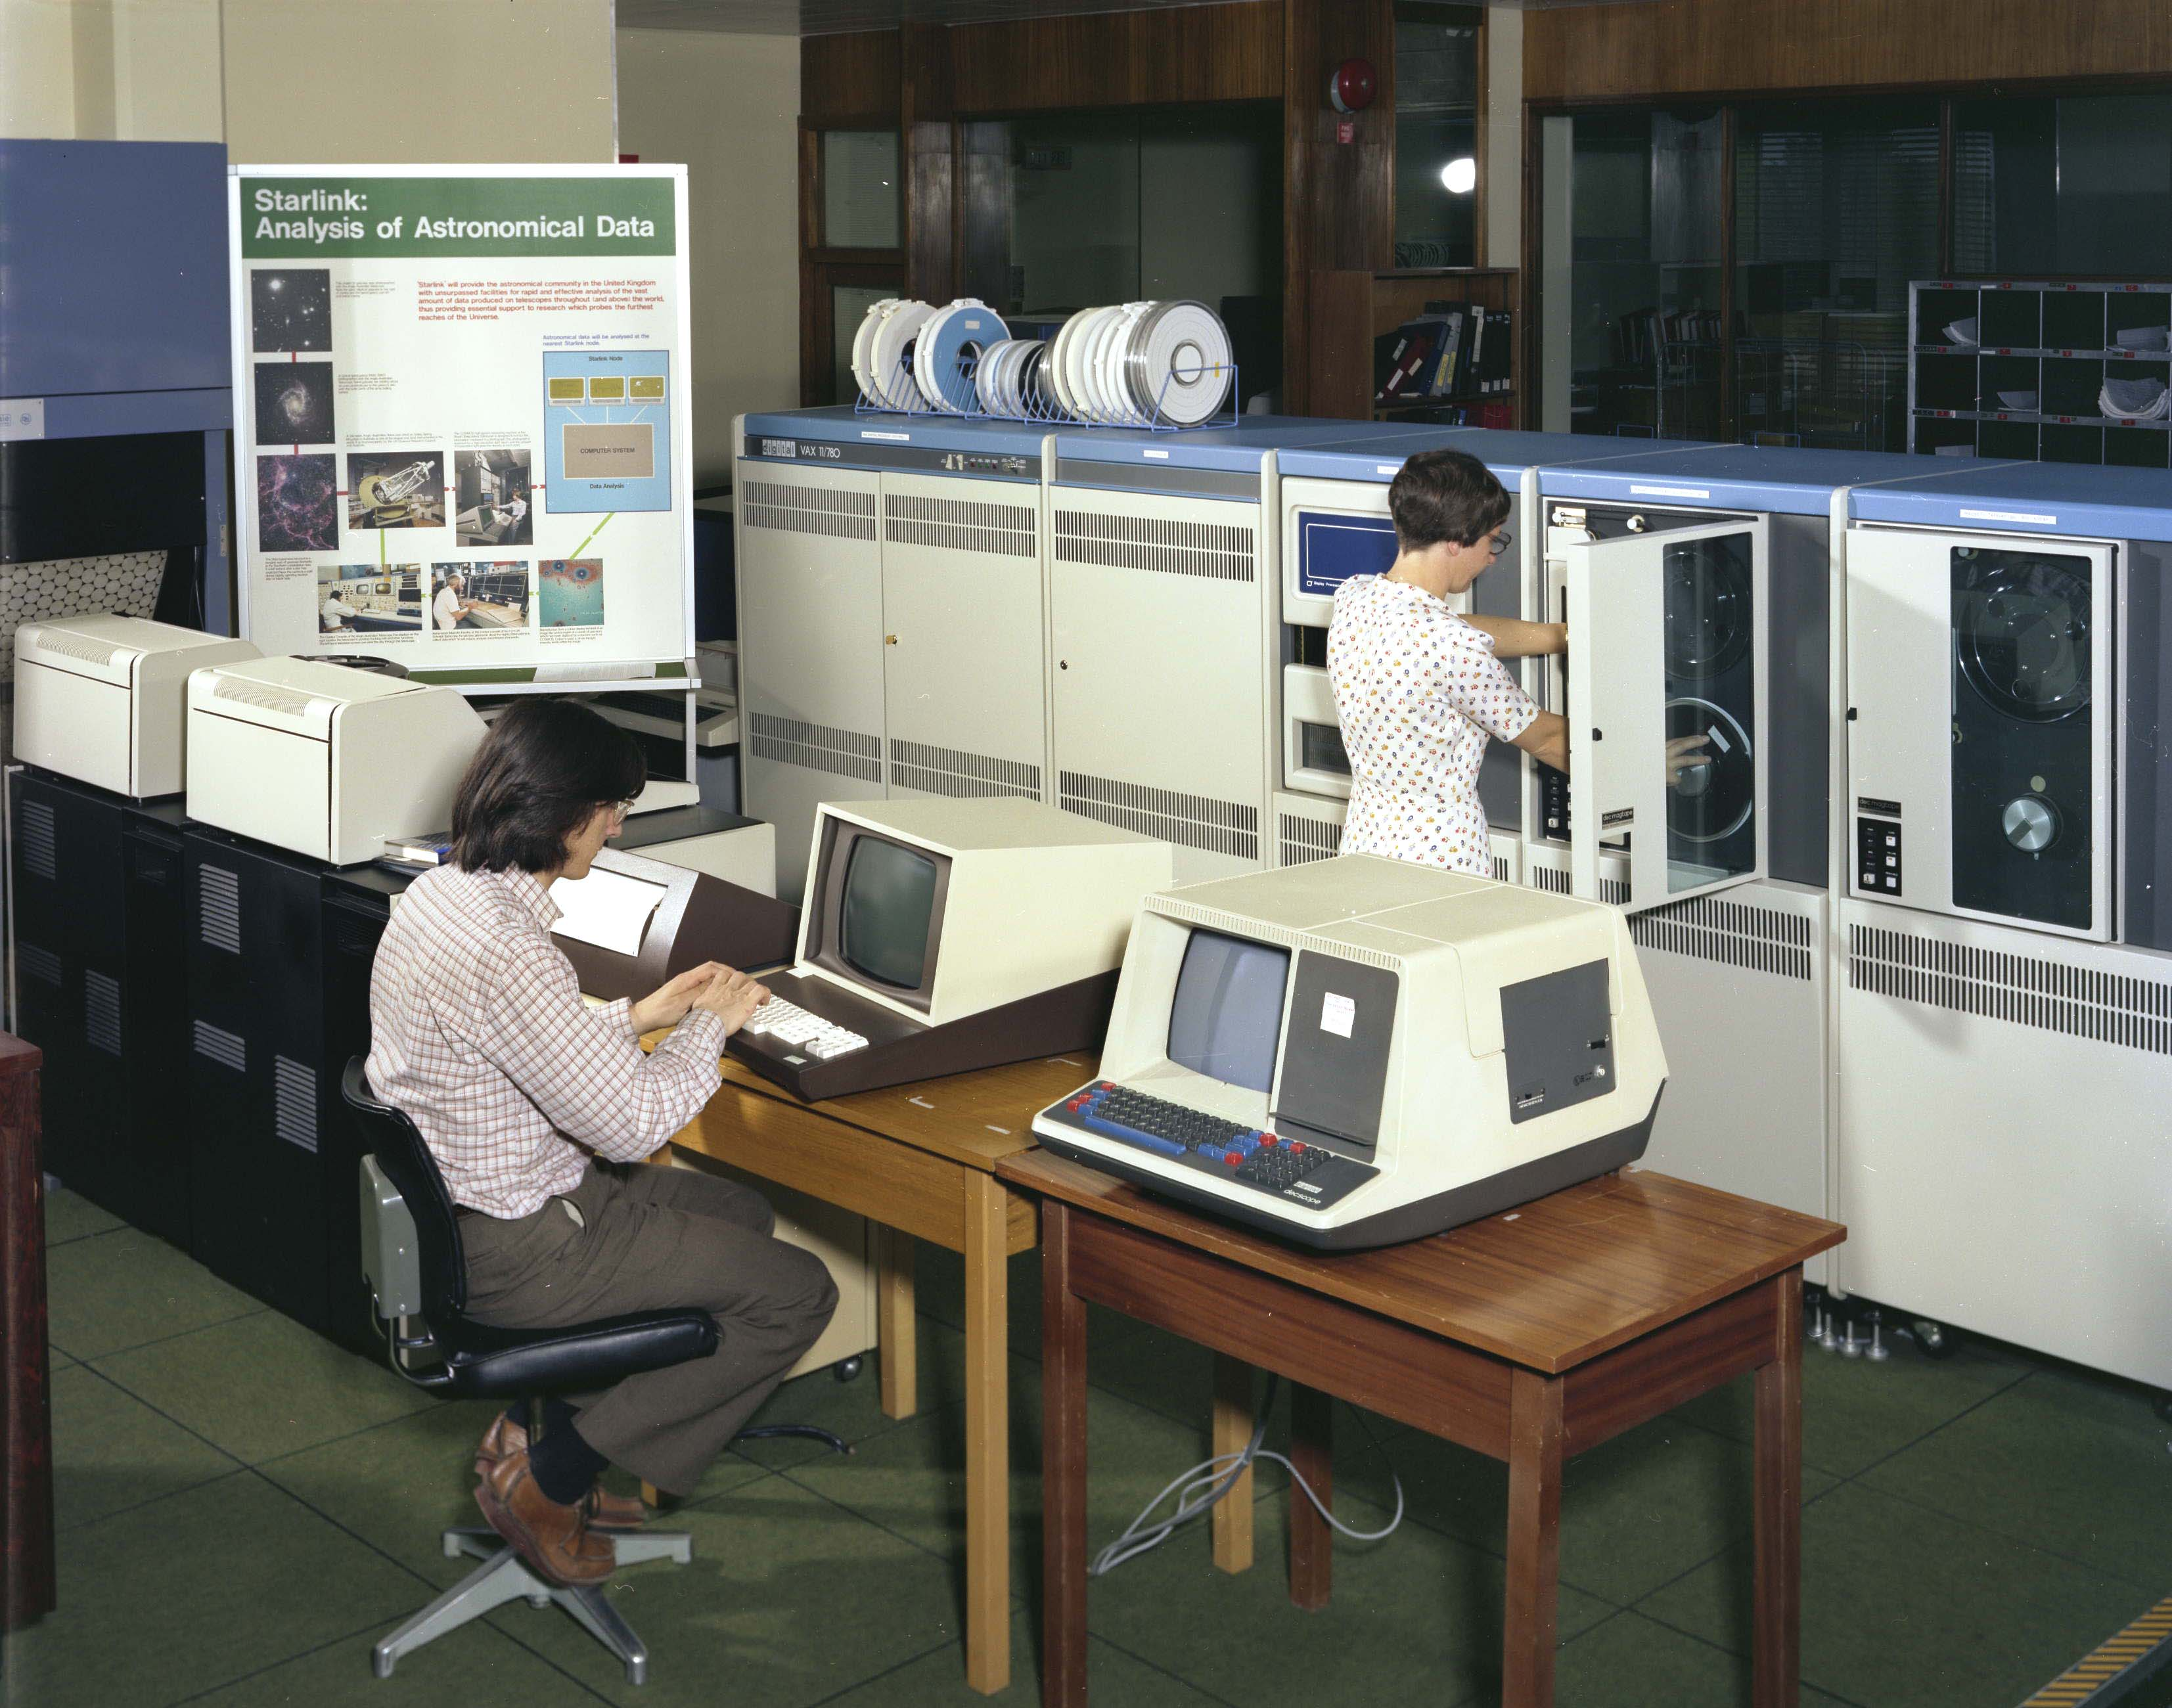
\includegraphics[keepaspectratio]{media/C03_historia/dec_vax11.jpg}
\caption{Instalación de VAX 11/780 en 1980 --- Fuente:
\href{http://www.chilton-computing.org.uk/}{Science and Technology
Facilities Council}}\label{fig-dec-vax11}
\end{figure}

Las siglas VMS vienen de \emph{Virtual Memory System}, ya que una de sus
principales características era explotar el concepto de \textbf{memoria
virtual}. Este concepto también es muy utilizado en los sistemas
operativos modernos. Permite que los procesos se ejecuten aislados, unos
de otros, en la memoria principal y sin tener que ser cargados
completamente, lo que permite que cada uno consuma menos memoria.

VMS era un sistema multiusuario y multiprocesador que podía distribuir
el trabajo entre varias máquinas, lo que le permitía ser tolerante a
fallos.

VMS es en cierta medida un ancestro de Microsoft Windows NT (véase el
\hyperref[sect-windows-nt]{Windows NT, 2000, XP, Vista, 7, 8 y 10}).
Para desarrollar Windows NT, Microsoft contrató a un grupo de
desarrolladores de Digital Equipment Corporation. Muchos aspectos del
diseño de Windows NT reflejan la experiencia de DEC en VMS.

\subsection{IBM OS/400}\label{_ibm_os400}

El \href{https://es.wikipedia.org/wiki/OS/400}{IBM OS/400} es un sistema
utilizado en la familia de minicomputadoras
\href{https://es.wikipedia.org/wiki/AS/400}{IBM AS/400} ---llamada
iSeries desde 2006---. Fueron introducidos en el mercado en 1988, pero
aún es posible verlos en algunas organizaciones. En 2008 el sistema
operativo IBM OS/400 pasó a llamarse IBM i y siguen publicándose nuevas
versiones en la actualidad.

\section{5ª Generación (desde
1980):}\label{sect-historia-quinta-generaciuxf3n}

Esta última generación abarca desde la década de 1980 hasta la
actualidad.

Respecto a los sistemas operativos:

\begin{itemize}
\item
  Incluye a los sistemas operativos de escritorio y ordenadores
  personales (PC).
\item
  Aparecen múltiples conceptos nuevos: monousuario, multitarea,
  distribuidos, paralelos, tiempo real, etc.
\end{itemize}

Se puede observar una muestra de la interfaz gráfica de usuario de
algunos de estos sistemas en el artículo
\href{https://www.webdesignerdepot.com/2009/03/operating-system-interface-design-between-1981-2009/}{«Operating
System Interface Design Between 1981-2009»}.

\subsection{CP/M}\label{_cpm}

\href{https://en.wikipedia.org/wiki/CP/M}{CP/M} (1974) fue el sistema
operativo estándar en la primera generación de microcomputadoras. Fue
creado por Digital Research, Inc. ---fundada por Gary Kildall--- para
ser el sistema operativo de los microordenadores basados en
\href{https://es.wikipedia.org/wiki/Intel_8080}{Intel 8080/85} y
\href{https://es.wikipedia.org/wiki/Zilog_Z80}{Zilog Z80}.

Con la elección de MS-DOS por parte de IBM para su \{ibmpc\}, CP/M fue
perdiendo mercado paulatinamente hasta desaparecer. Sin embargo, la
influencia de CP/M en MS-DOS es indudable, en tanto en cuanto 86-DOS, el
predecesor de MS-DOS, estaba basado en las ideas de CP/M.

\subsection{MS-DOS}\label{_ms_dos}

\{msdos\} fue el sistema operativo estándar en la segunda generación de
microcomputadoras. No era ni multitarea ni multiusuario. Fue el primer
sistema operativo del \{ibmpc\} ---lanzado en 1981--- y durante mucho
tiempo fue ampliamente utilizado en toda la plataforma «PC compatible».

MS-DOS fue creado por Seattle Computer Products (SCP) con el nombre de
\href{https://es.wikipedia.org/wiki/QDOS}{86-DOS} en 1979. Se basaron en
ideas de CP/M, pues pretendían ofrecer una versión de CP/M para
procesadores \{intel8086\}. Inicialmente era conocido como QDOS
(\emph{Quick and Dirty Operating System}) pero SCP le cambió el nombre
en 1980, cuando comenzaron a licenciarlo. Posteriormente Microsoft
adquirió el sistema y lo vendió a IBM en 1981 con el nombre de MS-DOS.

Tanto IBM como Microsoft lanzaron versiones de DOS, aunque originalmente
IBM solamente validaba y empaquetaba el software de Microsoft. Microsoft
lanzaba sus versiones bajo el nombre de MS-DOS, mientras IBM las lanzaba
bajo el nombre de \href{https://es.wikipedia.org/wiki/IBM_PC_DOS}{IBM
PC-DOS}.

En \href{https://www.pcjs.org/}{PCjs} se pueden probar de forma sencilla
sistemas operativos y aplicaciones antiguas del IBM PC. Solo hace falta
acceder con el navegador y elegir la experiencia que más nos llame la
atención.

\subsection{OS/2}\label{_os2}

\{os2\} fue un sistema operativo creado por Microsoft e IBM para
aprovechar las nuevas características de la segunda generación de
ordenadores personales de IBM, equipados con procesador
\href{https://es.wikipedia.org/wiki/Intel_80286}{Intel 80286}. Pero al
final terminó siendo desarrollado en exclusiva por IBM.

OS/2 fue pensado como un sucesor con \textbf{operación en modo dual} de
MS-DOS y de Microsoft Windows 2.0. Fue anunciado en abril y lanzado en
diciembre de 1987 como un sistema operativo en modo texto. En la versión
1.1, lanzada en noviembre de 1988, se le añadió interfaz gráfica.

\begin{figure}
\centering
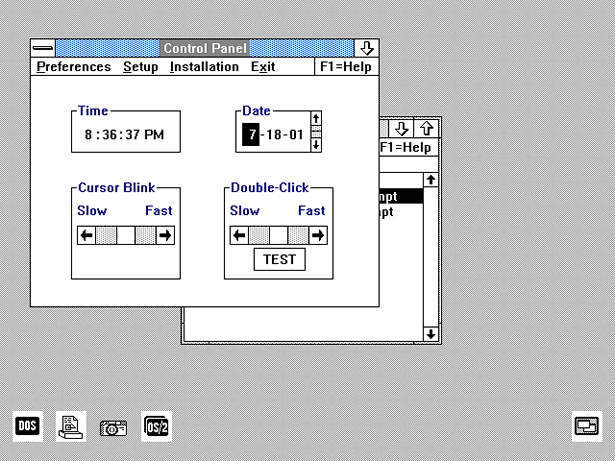
\includegraphics[keepaspectratio]{media/C03_historia/os_2_1.png}
\caption{Panel de control de Microsoft-IBM OS/2 1.1 --- Fuente: Michal
Necasek}\label{fig-os-21}
\end{figure}

En los sistemas con \textbf{operación en modo dual} se distingue entre
dos modos de ejecución, de tal forma que solo en el modo en el que se
ejecuta el código del sistema operativo se pueden realizar operaciones
peligrosas. En el otro modo y con menos privilegios, se ejecutan las
aplicaciones de usuario. Para más información, véase el
\hyperref[_operaciuxf3n_en_modo_dual]{???}

La colaboración entre IBM y Microsoft terminó en 1990, entre el
lanzamiento de Windows 3.0 y la de OS/2 1.3. El aumento de popularidad
de Windows llevó a Microsoft a dejar de centrarse en el desarrollo de
OS/2, lo que hizo que IBM se preocupara por los continuos retrasos en el
desarrollo de OS/2 2.0. Inicialmente ambas compañías acordaron que IBM
tomaría el mantenimiento de OS/2 1.0 y el desarrollo de OS/2 2.0,
mientras Microsoft continuaría desarrollando OS/2 3.0, que entonces era
conocido como «NT OS/2». Sin embargo, Microsoft finalmente decidió
renombrar NT OS/2 como Windows NT, dejando el futuro desarrollo de OS/2
en manos de IBM.

OS/2 Warp 3 fue un sistema completo de 32 bits lanzado en 1994. Le
seguiría OS/2 Warp 4, en 1996. Poco después, IBM anunció que OS/2
desaparecería.

\subsection{Windows 3.x}\label{_windows_3_x}

La familia \href{https://es.wikipedia.org/wiki/Windows_3.1x}{Windows
3.x} de Microsoft Windows fue desarrollada desde 1990 hasta 1994.
Windows 3.0 fue la primera versión de éxito de Windows, permitiendo a
Microsoft competir con el
\href{https://es.wikipedia.org/wiki/Macintosh}{Macintosh} de Apple
Computer y el
\href{https://es.wikipedia.org/wiki/Commodore_Amiga}{Commodore Amiga}.

\begin{figure}
\centering
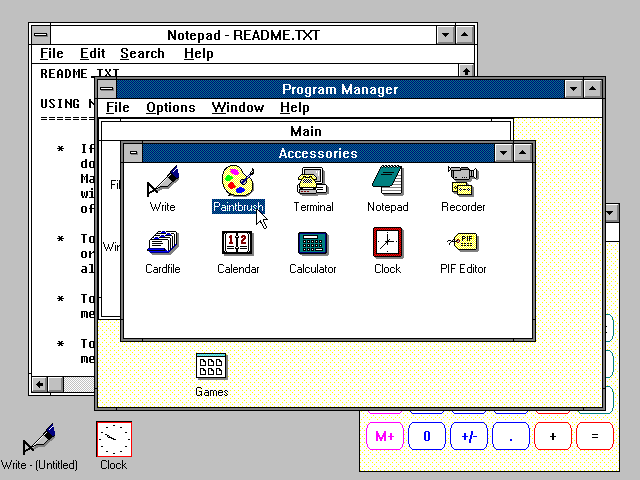
\includegraphics[keepaspectratio]{media/C03_historia/windows_30.png}
\caption{Administrador de programas de Microsoft Windows 3.0 --- Fuente:
\href{https://guidebookgallery.org/screenshots/win30}{Guidebook}}\label{fig-windows-30}
\end{figure}

En 1983, Microsoft anunció el desarrollo de Windows, una interfaz
gráfica de usuario para su sistema MS-DOS, que se usaba en los IBM PC y
compatibles desde 1981. Windows requería una instalación previa de
MS-DOS y era iniciado como un programa más, que podía ser terminado en
cualquier momento, devolviendo al usuario a la línea de comandos de
MS-DOS.

MS-DOS le proporcionaba a Windows controladores de dispositivo para
ciertas tareas, como el acceso al CD-ROM o a la interfaz de red. Sin
embargo Windows ejecutaba aplicaciones específicas de Windows,
almacenadas en un formato ejecutable mucho más complejo que el de los
programas de MS-DOS. Además, debido a que MS-DOS no aislaba a las
aplicaciones del hardware y no se protegía así mismo de los errores en
dichas aplicaciones, Windows disponía de controladores de dispositivo
propios, así como sus propios sistemas de gestión de procesos y de
memoria. En realidad Windows no se ejecutaba sobre MS-DOS, si no que
hacía uso de él. Por ello puede ser considerado como un sistema
operativo.

\subsection{Windows 95, 98, Me}\label{_windows_95_98_me}

La familia Windows 3.x fue sustituida por una serie de sistemas
operativos gráficos híbridos de 16/32 bits.

\begin{figure}
\centering
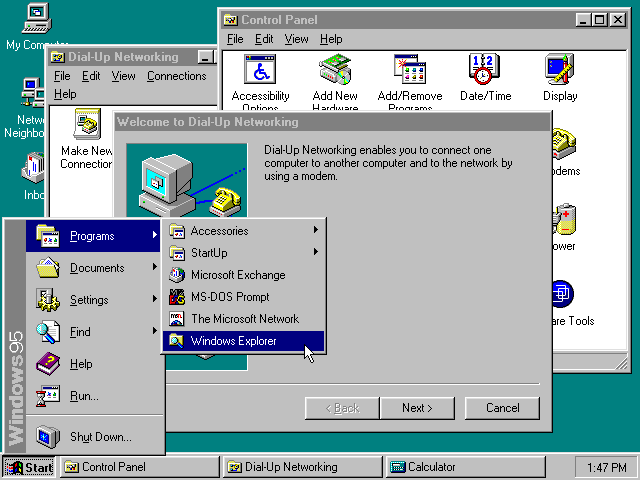
\includegraphics[keepaspectratio]{media/C03_historia/windows_95.png}
\caption{Escritorio de Microsoft Windows 95 --- Fuente:
\href{http://www.guidebookgallery.org/screenshots/win95}{Guidebook}}\label{fig-windows-95}
\end{figure}

Windows 95 fue lanzado en 1995. Fue el primer Windows unido a una
versión de MS-DOS específica, aunque este hecho se intentaba mantener
oculto. Entre las características de Windows 95 destacan: mejoras
significativas en la interfaz de usuario (véase la
\hyperref[fig-windows-95]{Escritorio de Microsoft Windows 95 --- Fuente:
}), nombres de archivo de hasta 256 caracteres con conservación de
mayúsculas y minúsculas ---en MS-DOS el límite era de 8 caracteres para
el nombre más 3 de extensión--- y multitarea expropiativa para las
aplicaciones de 32 bits.

Como veremos en el \hyperref[_planificaciuxf3n_expropiativa]{???}, la
planificación expropiativa es una técnica que permite al sistema
operativo expulsar de la CPU a los procesos en ciertas circunstancias;
como, por ejemplo, que llevan demasiado tiempo utilizando la CPU de
forma ininterrumpida.

En la familia Windows 3.x la planificación era cooperativa, es decir,
los procesos abandonaban la CPU voluntariamente. Esto ocasionaba
problemas con programas que no devolvía la CPU al sistema con la
suficiente frecuencia, ya que así el resto de procesos no tenía ocasión
de ejecutarse para hacer su trabajo o responder al usuario.

Windows 98 fue lanzado el 25 de junio de 1998. Le siguió Windows Me, el
14 de septiembre de 2000. Windows Me fue la última versión de la familia
de sistemas operativos híbridos de 16/32 bits que sucedió a la familia
Windows 3.x.

\subsection{Windows NT, 2000, XP, Vista, 7, 8 y
10}\label{sect-windows-nt}

Windows NT fue un sistema operativo de 32 bits. El primero de la familia
de sistemas operativos Microsoft Windows actuales.

Su desarrollo empezó en 1988 con el nombre de OS/2 3.0. Cuando Windows
3.0 fue lanzado en mayo de 1990, tuvo tanto éxito que Microsoft decidió
cambiar la API del aún en desarrollo NT OS/2 ---que era como Microsoft
lo llamaba entonces--- pasando de ser una versión extendida de la API de
OS/2 a una versión extendida de la API de Windows 3.0. Esta decisión
causó tensión entre Microsoft e IBM y provocó que finalmente terminara
la colaboración.

Una interfaz de programación de aplicaciones o API (del inglés
\emph{Application Programming Interface}) es el conjunto de funciones,
procedimientos o métodos que ofrece el sistema operativo para ser
utilizado por las aplicaciones.

Como hemos comentado anteriormente, Microsoft contrató a un grupo de
desarrolladores de Digital Equipment Corporation para crear Windows NT.
Por lo que muchos de sus elementos reflejan la experiencia anterior de
DEC en VMS.

Windows NT soportaba varias API de distintos sistemas operativos ---por
ejemplo Win32, POSIX y OS/2 2.1--- que eran implementadas como
subsistemas encima de una API nativo no documentado públicamente. Esta
estructura en subsistemas, fue lo que permitió la adopción tardía de la
API de Windows 3.0 como API principal, tal y como hemos comentado.

La primera versión ---Windows NT 3.1--- lanzada el 13 de julio de 1993,
era un sistema operativo \emph{microkernel} (véase el
\hyperref[_mach]{Mach} un poco más adelante) multiplataforma que corría
sobre procesadores \{x86\}, \{decalpha\}, \{mips\} 4000 y
\href{https://es.wikipedia.org/wiki/PowerPC}{PowerPC}.

Windows NT 4.0 ---lanzado en 1996--- fue la última versión en soportar
plataformas distintas a Intel IA-32. Aunque el desarrollo de Windows
2000 para procesador Alpha continuó un poco más, hasta 1999, cuando
Compaq dejó de soportar Windows NT en esa arquitectura. Además Windows
NT 4.0 integró en el núcleo más funciones ---por ejemplo, parte del
subsistema gráfico--- para obtener un rendimiento más próximo al de
Windows 95 en ese apartado.

Windows 2000 ---o Windows NT 5.0--- fue lanzado el 17 de febrero de 2000
y fue el primer sistema operativo de la familia NT al que se le
eliminaron las siglas del nombre. Fue por motivos de marketing, para
favorecer la unificación de las dos familias de sistemas operativos
Microsoft Windows de entonces ---Windows 9x y Windows NT--- alrededor de
la tecnología NT.

Windows XP ---o Windows NT 5.1--- completó en 2001 el proceso de
unificación de las dos familias de sistemas operativos Windows. Con su
aparición forzó la extinción de la familia Windows 9x, al sustituirla
con una versión de Windows XP denominada Windows XP Home Edition,
específica para la informática doméstica.

\subsection{GNU/Linux}\label{_gnulinux}

\{gnulinux\} es un sistema operativo libre y, tal vez, el más famoso
proyecto de \href{https://es.wikipedia.org/wiki/Software_libre}{software
libre}.

El proyecto GNU se inició en 1983, con el fin de desarrollar un sistema
operativo estilo UNIX enteramente libre. El proyecto incluía la creación
de herramientas de desarrollo de software y aplicaciones de usuario.

Mucho tiempo después, el estudiante universitario finés Linus Torvalds
comenzó a desarrollar el núcleo Linux como hobby, mientras estudiaba en
la Universidad de Helsinki. Torvalds originalmente usaba \{minix\}, un
sistema operativo simplificado escrito por Andrew Tanenbaum para enseñar
diseño de sistemas operativos. Sin embargo, el hecho de que Tanenbaum no
diera soporte a las mejoras del sistema operativo que eran propuestas
por otros desarrolladores, llevó a Torvalds a escribir un sustituto de
MINIX.

En 1991, cuando se liberó la primera versión del núcleo Linux, el
proyecto GNU había desarrollado todos los componentes necesarios del
sistema operativo excepto el núcleo. Torvalds y otros desarrolladores
rápidamente adaptaron Linux para que funcionara con los componentes de
GNU, creando un sistema operativo completamente funcional que se
denomina GNU/Linux.

El núcleo Linux fue licenciado bajo la GNU General Public License (GPL),
como el resto del proyecto GNU. Pero Linux no es parte de dicho
proyecto. El proyecto GNU tiene su propio núcleo, denominado
\{gnuhurd\}, que lleva 30 años en desarrollo y parece que aún está muy
lejos de estar listo.

GNU no es el único sistema operativo que utiliza el núcleo Linux.
\{android\}, por ejemplo, es un sistema operativo que usa el núcleo
Linux, pero no es GNU.

\subsection{Mach}\label{_mach}

\{mach\} es un núcleo de sistema operativo desarrollado en la
Universidad Carnegie-Mellon (CMU). El proyecto en la CMU se desarrolló
desde 1985 hasta 1994.

Mach explora el concepto que denominamos \textbf{\emph{microkernel}}. En
los sistemas operativos \textbf{\emph{microkernel}} solo se implementa
en el núcleo del sistema un conjunto mínimo de servicios básicos. El
resto de los servicios proporcionados por el sistema operativo se
implementan como procesos con menos privilegios.

Por sus ventajas en cuanto a seguridad y fiabilidad, en algún momento se
pensó que los \emph{microkernel} dominarían el universo de los sistemas
operativos. Sin embargo, el mayor esfuerzo hasta la fecha para
conseguirlo es \{gnuhurd\}, que lleva varias décadas de retraso. Por
fortuna, otros sistemas operativos \emph{microkernel} han tenido algo
más éxito, como es el caso de \{qnx\} o \{minix3\}. Mientras que Google
parece que lo va a intentar con \{google\_fuchsia\}, el posible
sustituto de Android.

A mediados de los 90, Apple Computers seleccionó
\href{https://es.wikipedia.org/wiki/NEXTSTEP}{OpenStep} como base para
el sucesor de su clásico
\href{https://es.wikipedia.org/wiki/Mac_OS_Classic}{Mac OS}. OpenStep es
realmente una versión actualizada de NeXTSTEP que era un sistema basado
en un núcleo Mach 2.5 con porciones del sistema UNIX BSD de la
Universidad de Berkeley. Por tanto, la mezcla de Mach con UNIX BSD de
OpenStep es la base del sistema operativo \{macos\} actual de Apple.

\begin{figure}
\centering
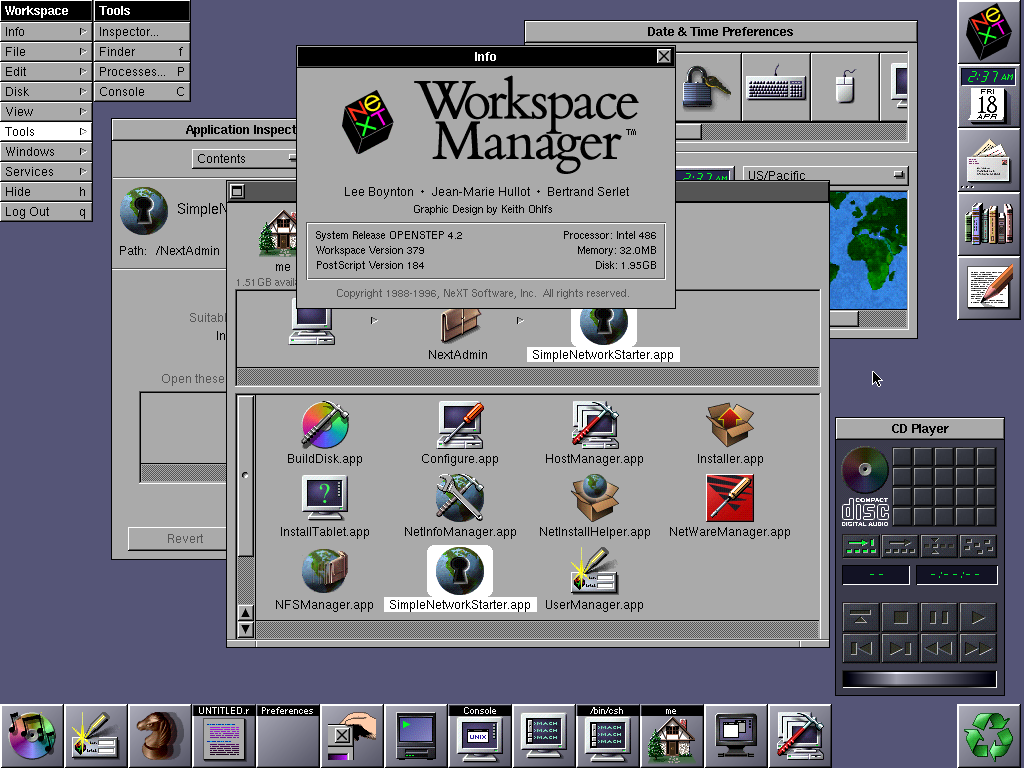
\includegraphics[keepaspectratio]{media/C03_historia/openstep_42.png}
\caption{Entorno gráfico de OpenStep 4.2 --- Fuente:
\href{https://guidebookgallery.org/screenshots/openstep42}{Guidebook}}\label{fig-openstep-42}
\end{figure}

Para ser exactos, la base del sistema operativo macOS es un sistema
operativo libre denominado \{darwin\} y desarrollado por Apple. Se trata
de un sistema \{freebsd\} adaptado para correr sobre el núcleo Mach.

\begin{figure}
\centering
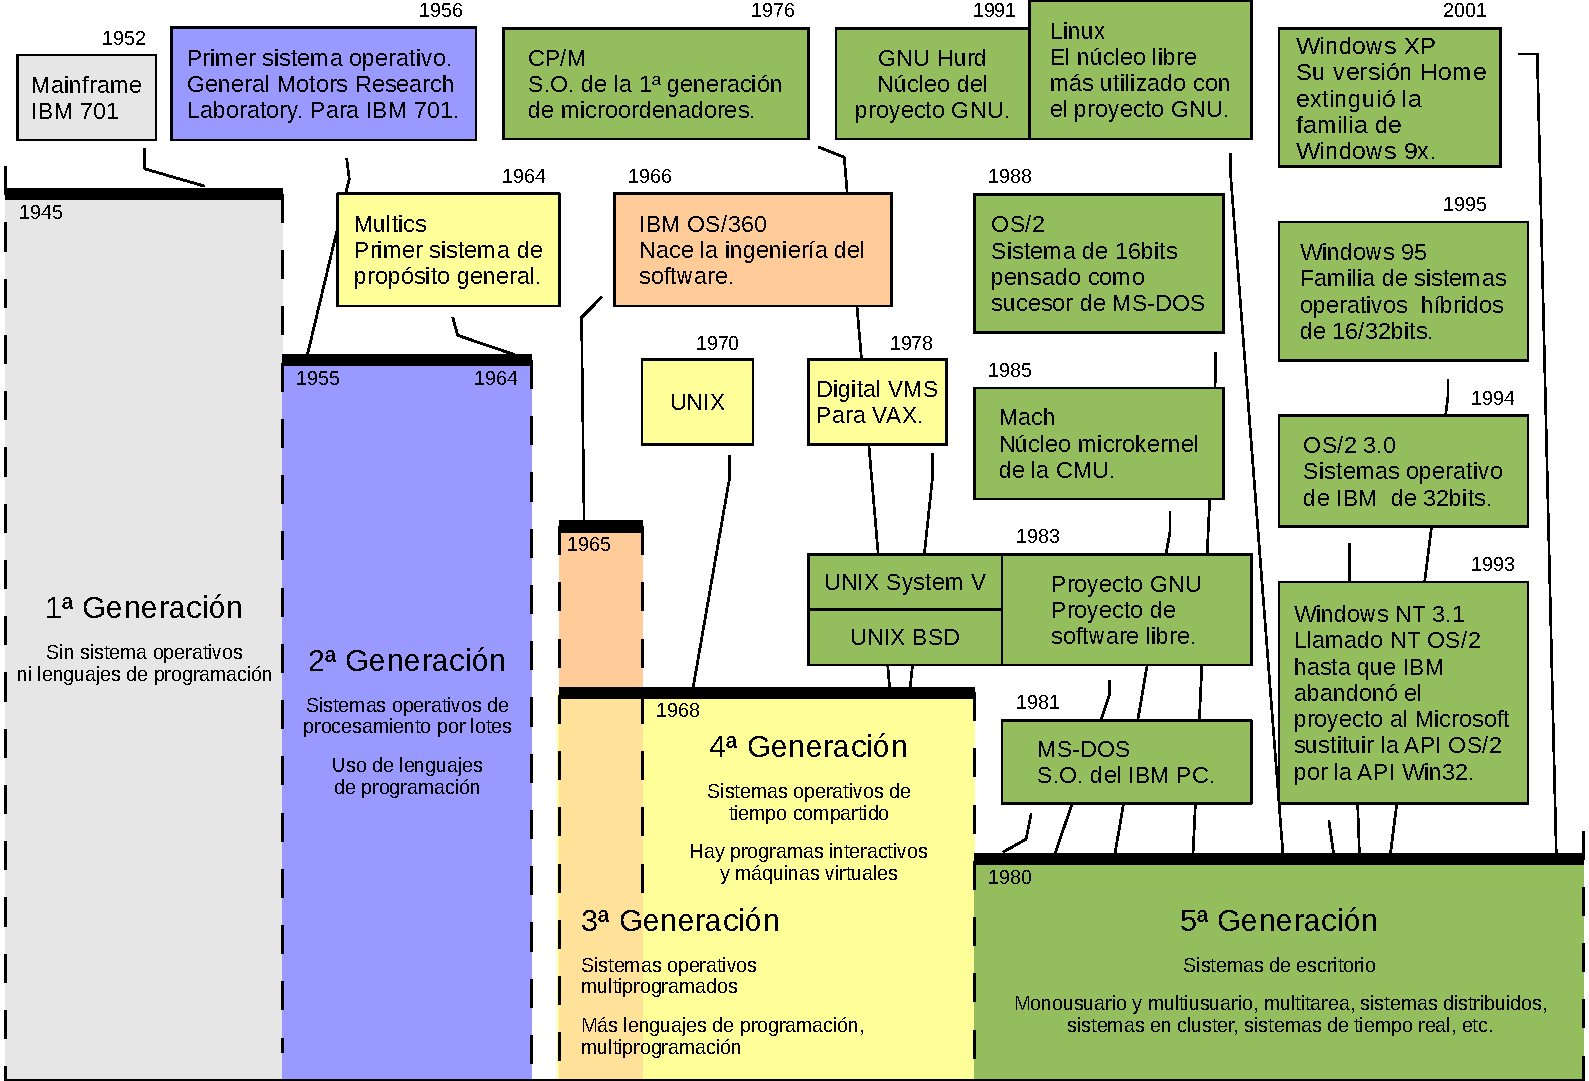
\includegraphics[width=0.8\textwidth]{media/C03_historia/historia_sistemas_operativos.pdf}
\caption{Línea de tiempo de la historia de los sistemas operativos.}
\end{figure}


% ── Parte II: Organización ───────────────────────────────
\part{Organizaci\'{o}n de los sistemas operativos}
\input{partes/P02_preambulo}
\include{capitulos/C04_componentes}
\include{capitulos/C05_servicios}
\include{capitulos/C06_api}
\section{}

\textbf{Tiempo de lectura:} \{s07-reading-time\}

Dado que el sistema operativo y los procesos de usuarios comparten los
recursos del sistema informático, necesitamos estar seguros de que un
error en un programa solo afecte al proceso que lo ejecuta ---por
ejemplo, que un proceso no puede modificar la memoria de otro proceso o
la del núcleo del sistema---. Por eso es necesario establecer mecanismos
de protección frente a los errores en los programas que se ejecutan en
el sistema.

\section{Software controlado mediante
interrupciones}\label{_software_controlado_mediante_interrupciones}

Antes de entender cómo funcionan estos mecanismos de protección debemos
entender que los sistemas operativos modernos pertenecen a un tipo de
software que se dice que está controlado mediante interrupciones.

Los sucesos que requieren la atención del sistema casi siempre se
indican mediante una interrupción:

\begin{itemize}
\item
  Cuando un proceso comete un error ---como una división por cero o un
  acceso a memoria no válido--- lo que se genera es una excepción en la
  CPU. Esta excepción despierta al sistema operativo para que haga lo
  que sea más conveniente.
\item
  Cuando un proceso necesita un servicio lo que hace es lanzar una
  llamada al sistema, que no es más que ejecutar una instrucción que
  lanza una excepción en la CPU. Esta excepción despierta al sistema
  operativo para que atienda la petición.
\item
  Cuando los dispositivos de E/S requieren la atención del sistema
  operativo ---por ejemplo, porque se ha completado una transferencia de
  datos--- se genera una interrupción en la CPU, que despierta al
  sistema operativo.
\end{itemize}

Esto funciona así porque el sistema operativo configura la CPU durante
el arranque para que si ocurre cualquier interrupción o excepción la
ejecución, salte a rutinas en el código del núcleo, con el objeto de
darles el tratamiento adecuado.

Si ningún proceso realiza una acción ilegal o pide un servicio, ni
ningún dispositivo de E/S pide la atención del sistema, el sistema
operativo permanece inactivo esperando a que algo ocurra.

Teniendo todo esto en cuenta podremos entender mejor cómo funciona el
modo dual.

\section{Operación en modo dual}\label{_operaciuxf3n_en_modo_dual}

Para proteger el sistema de programas con errores es necesario poder
distinguir entre la ejecución del código del sistema operativo y del
código de los programas de usuario, de tal forma que el código de los
programas de usuario esté más limitado en lo que puede hacer que el del
sistema operativo.

El método que utilizan la mayor parte de los sistemas operativos
consiste en utilizar algún tipo de soporte en la CPU que permita
diferenciar entre varios modos de ejecución y restringir la utilización
de las instrucciones peligrosas ---llamadas \textbf{instrucciones
privilegiadas}{}--- para que solo puedan ser utilizadas en el modo en el
que se ejecuta el código del sistema operativo.

\subsection{Modos de operación}\label{_modos_de_operaciuxf3n}

Así que como mínimo son necesarios dos modos de operación diferentes:

\begin{itemize}
\item
  En el \textbf{modo usuario}{}, en el que se ejecuta el código de los
  procesos de los usuarios. Si se hace un intento de ejecutar una
  instrucción privilegiada en este modo, el hardware la trata como
  ilegal y genera una excepción que es interceptada por el sistema
  operativo, en lugar de ejecutar la instrucción.
\item
  En el \textbf{modo privilegiado}{} ---también denominado \textbf{modo
  supervisor}{}, \textbf{modo del sistema}{} o \textbf{modo kernel}{}---
  se ejecuta el código de las tareas del sistema operativo. La CPU es la
  encargada de garantizar que las instrucciones privilegiadas solo
  pueden ser ejecutadas en este modo.
\end{itemize}

El modo actual de operación puede venir indicado por un \textbf{bit de
modo}{} en alguno de los registros de configuración de la CPU, de tal
forma que, si por ejemplo, el bit está a 0, la CPU considera que el
código en ejecución opera en modo privilegiado, mientras que si el bit
está a 1, el código en ejecución opera en modo usuario.

Comúnmente en el grupo de las \textbf{instrucciones privilegiadas} se
suelen incluir:

\begin{itemize}
\item
  La instrucción para conmutar al modo usuario desde el modo
  privilegiado.
\item
  Las instrucciones para acceder a dispositivos de E/S.
\item
  Las instrucciones necesarias para la gestión de las interrupciones.
  Por ejemplo, para desactivarlas ---evitando que se lancen---
  activarlas y configurarlas.
\end{itemize}

Aunque para operar en modo dual solo se necesita que la CPU admita los
dos modos descritos, existen procesadores que soportan más, con la idea
de tener mayor control sobre el nivel de privilegio en el que se ejecuta
cada componente del sistema.

Es el caso de la arquitectura Intel x86, que soporta 4 modos de
operación\hyperref[Wikipedia-Anillo]{???}. El modo 0 es para el software
más confiable y el que necesita más privilegios, que generalmente es el
núcleo. Mientras que el modo 3 se utiliza para el software menos
confiable y que necesita más supervisión, que normalmente son los
procesos de usuario.

La idea detrás de tener los modos 1 y 2 es usarlos para controladores de
dispositivo o procesos que dan servicio al resto del sistema. Así estos
componentes pueden tener mayores privilegios que los procesos de usuario
---por ejemplo, los controladores de dispositivo necesitan acceso
directo al hardware--- pero al mismo tiempo serían supervisados y no
podrían afectar al núcleo, que se ejecuta en el modo 0.

Sin embargo, los sistemas operativos con mayor cuota de mercado
---incluyendo Microsoft Windows, macOS, Linux y Android--- solo utilizan
los modos 0 y 3. Los motivos son que los desarrolladores de sistemas no
encuentran realmente ninguna ventaja en utilizar más modos y que
complica portar el sistema operativo a procesadores donde solo se
soporten dos.

En procesadores x86 recientes, que vienen con instrucciones específicas
para facilitar la ejecución de máquinas virtuales, se ha incorporado un
modo -1, para que el núcleo del sistema operativo virtualizado se
ejecute en el modo 0 mientras es supervisado desde el modo -1 por el
núcleo del sistema operativo anfitrión.

En los procesadores x86 es importante no confundir los \textbf{modos
real}{} y \textbf{protegido}{} con el modo dual y los niveles de
privilegio de los que estamos hablando.

Por compatibilidad hacia atrás, los procesadores x86 se inician en modo
real, donde se comportan como una CPU \{intel8086\}. En este modo, por
ejemplo, solo tienen acceso al primer mega de memoria RAM ---ya que los
procesadores \{intel8086\} solo tenían 20 bits para direcciones de
memoria---.

Cuando un sistema operativo moderno arranca, lo primero que hace es
iniciar el modo protegido, en el que se activan todas las
características de la CPU. Entre otras, el direccionamiento de 32 o 64
bits ---según el procesador que sea--- y la posibilidad de usar los 4
niveles de privilegio, de los que hemos hablado, para que el núcleo
pueda supervisar al resto de componentes.

\subsection{Ejecución de
instrucciones}\label{_ejecuciuxf3n_de_instrucciones}

A continuación podemos ver el ciclo de vida de la ejecución de
instrucciones en un sistema con modo dual de operación:

\begin{enumerate}
\def\labelenumi{\arabic{enumi}.}
\item
  Inicialmente, al arrancar el ordenador, la CPU se inicia en el modo
  privilegiado ---es decir, en nuestro ejemplo, con el bit de modo a
  0---. En este modo se carga el núcleo del sistema operativo e inicia
  su ejecución.
\item
  El núcleo del sistema operativo debe cambiar al modo usuario
  ---poniendo el bit de modo a 1--- antes de ceder la CPU a un proceso
  de usuario. Esto ocurre cuando es necesario que un proceso de usuario
  continúe o inicie su ejecución (véase el
  \hyperref[_el_asignador]{???}). Así se asegura que el código de los
  procesos de usuario siempre se ejecuten en modo usuario, con menos
  privilegios.
\item
  La CPU conmuta a modo privilegiado cuando ocurre una interrupción o
  una excepción ---poniendo el bit de modo a 0--- antes de comenzar el
  código del sistema operativo que se encargará de tratarlas.
\end{enumerate}

Esto último es muy importante. Como ya hemos comentado, los sistemas
operativos están controlados mediante interrupciones. Al activarse el
modo privilegiado cada vez que ocurre una interrupción, podemos estar
seguros de que las tareas del sistema operativo se ejecutarán siempre en
modo privilegiado.

Cuando se dispone de la protección del modo dual, el hardware se encarga
de detectar los errores de ejecución y de notificarlo al sistema
operativo mediante excepciones, siendo responsabilidad de este último
realizar un tratamiento adecuado de los mismos. Por lo general, si un
programa falla de alguna forma ---como por ejemplo, intentando utilizar
una instrucción ilegal o de acceder a una zona de memoria inválida--- el
sistema operativo lo hace terminar.

\section{Protección de la memoria}\label{_protecciuxf3n_de_la_memoria}

La memoria principal debe acomodar tanto el sistema operativo como a los
diferentes procesos de los usuarios. Por eso la memoria normalmente se
divide en dos partes o espacios:

\begin{enumerate}
\def\labelenumi{\arabic{enumi}.}
\item
  La primera parte es el \textbf{espacio del núcleo}{}. Sirve para
  albergar el núcleo del sistema operativo.

  El sistema operativo puede estar localizado tanto en la parte baja
  como en la parte alta de la memoria. El factor determinante es la
  dirección de memoria a la que salta la CPU cuando ocurre una
  interrupción o la dirección del vector de interrupciones ---que es una
  tabla en la memoria donde se definen las direcciones a las que saltará
  la CPU en caso de que ocurra una interrupción o una excepción--- según
  esté definido en la arquitectura correspondiente.

  En los procesadores de la familia x86, el vector de interrupciones
  reside en la dirección 0x00000000 y ocupa 0x400 bytes, por lo que,
  normalmente, el sistema operativo se aloja en la parte baja de la
  memoria. Sin embargo, en los procesadores MIPS las interrupciones se
  manejan saltando a la dirección 0x80000180, que está en la mitad del
  espacio de direcciones, en procesadores de 32 bits. Por tanto, lo más
  probable es que se aloje el sistema operativo por encima de la
  dirección 0x80000000.
\item
  La segunda parte es el \textbf{espacio de usuario}{} y alberga los
  procesos de usuario.
\end{enumerate}

Sin embargo, en los sistemas operativos modernos, los procesos no tienen
acceso libre a toda memoria física, con el objeto de proteger a los
procesos en ejecución y al sistema operativo de posibles errores en
cualquiera de ellos:

\begin{itemize}
\item
  El sistema operativo proporciona a cada proceso una «vista» privada de
  la memoria RAM; de tal forma que el \textbf{espacio de usuario} que ve
  cada proceso es similar al que vería cada uno de ellos si se estuviera
  ejecutando en solitario (véase la
  \hyperref[fig-protecciuxf3n-memoria]{Mapeo de la memoria física en el
  espacio de direcciones virtual de un proceso.}).
\item
  A esa «vista» que tiene cada proceso de la memoria es a lo que se
  denomina \textbf{espacio de direcciones virtual}{} del proceso. Está
  formada por el conjunto de todas las direcciones que puede generar la
  CPU para un proceso dado. Por ejemplo, en una CPU de 32 bits el
  espacio de direcciones virtual tiene 4 GiB, desde la dirección
  0x00000000 a 0xFFFFFFFF.
\item
  En los accesos a la memoria principal durante la ejecución del
  proceso, estas \textbf{direcciones virtuales}{} son convertidas por la
  CPU en direcciones físicas, antes de ser enviadas a la memoria
  principal. Por tanto las \textbf{direcciones físicas}{} son las
  direcciones reales que ve la memoria. Mientras que el \textbf{espacio
  de direcciones físico}{} es el conjunto de direcciones físicas que
  corresponden a todas las direcciones virtuales de un espacio de
  direcciones virtual dado.
\end{itemize}

\begin{figure}
\centering
\includegraphics[width=0.8\textwidth]{media/C07_modo_dual/protección_memoria.pdf}
\caption{Mapeo de la memoria física en el espacio de direcciones virtual
de un proceso.}\label{fig-protecciuxf3n-memoria}
\end{figure}

La conversión de una dirección virtual en una física, la realiza en
tiempo de ejecución un componente de la CPU denominado MMU
(\emph{Memory-Management Unit}).

Las ventajas de usar esta técnica, desde el punto de vista de la
protección de la memoria son:

\begin{itemize}
\item
  Permite el aislamiento de los procesos, creando para cada uno la
  ilusión de que toda la memoria es para él y evitando que un proceso
  pueda acceder a la memoria de otros procesos.
\item
  Permite marcar modos de acceso autorizados en las diferentes regiones
  de la memoria ---como por ejemplo lectura, escritura y ejecución---
  evitando que el código ejecutado en modo usuario tenga acceso a zonas
  a las que no debería tenerlo. El acceso a la memoria en un modo no
  autorizado se considera una instrucción privilegiada, por lo que ese
  tipo de acceso desde el modo usuario siempre genera una excepción. Por
  ejemplo, si se intenta ejecutar instrucciones en una zona de memoria
  no marcada con el permiso de ejecución.
\end{itemize}

\section{El temporizador}\label{_el_temporizador}

El \textbf{{}temporizador} se configura por el sistema operativo durante
el arranque del sistema para interrumpir a la CPU a intervalos
regulares. Así, cuando el temporizador interrumpe, el control se
transfiere automáticamente al núcleo del sistema. Entonces este puede:

\begin{itemize}
\item
  Conceder más tiempo al proceso en ejecución.
\item
  Detenerlo y darle más tiempo de CPU en el futuro
\item
  Tratar la interrupción como un error y terminar el programa.
\end{itemize}

El temporizador se utiliza para asegurar que ningún proceso acapara la
CPU indefinidamente. Por ejemplo, un programa mal desarrollado que entra
en un bucle infinito, del que no sale jamás.

Obviamente, las instrucciones que pueden modificar el contenido del
temporizador son instrucciones privilegiadas.

\section{Máquinas virtuales}\label{_muxe1quinas_virtuales}

{} Utilizando las técnicas comentadas anteriormente, el sistema
operativo crea a los procesos la ilusión de que se ejecutan en su propio
procesador y memoria principal, aunque realmente los estén compartiendo
con otros procesos. Obviamente, los procesos saben que hay un sistema
operativo que los supervisa, porque no pueden acceder directamente al
hardware, sino que deben solicitar los distintos recursos a través de
las llamadas al sistema.

Sin embargo, en algunos casos puede interesar que los procesos accedan a
los recursos a través de una interfaz de hardware virtual. Por ejemplo,
que un proceso, en lugar de hacer llamadas al sistema para pedir al
sistema operativo que lea cierto bloque de datos del disco duro, pueda
ejecutar directamente las instrucciones de E/S necesarias para pedir a
la controladora de disco que lea el bloque que le interesa y lo deposite
en la memoria, como si no estuviera siendo supervisado por el sistema
operativo.

Obviamente, no se trata de que el proceso tengo acceso a la controladora
real, sino que en el sistema hay un componente de software que ejecuta
una simulación de algún modelo de controladora de disco al que llegan
las peticiones del proceso. Como las instrucciones de E/S necesarias
para acceder al hardware son instrucciones privilegiadas, el sistema
operativo las intercepta ---gracias al apoyo del modo dual--- pero no
interpreta la situación como debida a un programa defectuoso, sino que
traslada la operación solicitada a los componentes de hardware virtual,
para luego continuar la ejecución del proceso en la siguiente
instrucción. El resultado es que el proceso tiene la ilusión de que se
ejecuta solo en una máquina vacía, con cierto hardware al que puede
acceder directamente, aunque este hardware realmente está siendo
simulado.

Los componentes de hardware virtual simulan el comportamiento de modelos
concretos de dispositivos hardware reales, implementando la
funcionalidad del hardware simulado con ayuda de otros componentes del
sistema operativo. Por ejemplo, una tarjeta de sonido virtualizada, en
última instancia usará los servicios del sistema operativo para
reproducir o grabar sonido usando el dispositivo real, mientras que el
controlador de disco virtualizado probablemente simulará las operaciones
de lectura y escritura trasladándolas a un archivo del sistema de
archivos real que hará de imagen del disco duro virtual.

Estos procesos que no se solicitan servicios al sistema operativo
mediante llamadas al sistema, si no haciendo uso de una interfaz de
hardware virtual, es lo que se conoce como máquinas virtuales. El
software de gestión de las máquinas virtuales es el responsable de
implementar los componentes de hardware virtual y de recibir del sistema
operativo los intentos de ejecutar instrucciones privilegiadas por parte
del código que se ejecuta dentro de las máquinas virtuales. Por tanto,
la operación en modo dual y las técnicas comentadas anteriormente en
este tema son fundamentales para implementar el soporte de máquinas
virtuales en los sistemas operativos modernos.

Una interfaz de hardware virtual es, por lo general, menos eficiente que
una basada en llamadas al sistema. A fin de cuentas, necesita que se
simule el hardware virtual mediante software, para luego traducir las
peticiones realizadas mediante esa interfaz en peticiones al sistema
operativo del sistema anfitrión. Una solución frecuente a este
inconveniente es la \textbf{paravirtualización}.

Por lo general, en la máquina virtual se ejecuta un sistema operativo,
que debe tener controladores de dispositivos para gestionar el acceso al
hardware virtual de la máquina. Es decir, los procesos que se ejecutan
en la máquina virtual solicitan servicios al sistema mediante llamadas
al sistema. El sistema operativo atiende esas peticiones usando los
recursos del hardware virtual, a los que accede mediante los
controladores de dispositivo correspondientes.

La \textbf{{}paravirtualización} consiste en instalar en el sistema
operativo de las máquinas virtuales controladores de dispositivo
desarrollados bajo la premisa de que se van a usar en una máquina
virtual. La particularidad es que estos controladores saben usar una
interfaz que provee el software de gestión de máquinas virtuales
---mediante un mecanismo similar a las llamadas al sistema--- para
trasladar las peticiones que llegan del sistema operativo en la máquina
virtual directamente al sistema operativo anfitrión, sin necesidad de
utilizar el hardware simulado.

\section{Arranque del sistema}\label{_arranque_del_sistema}

Desde el momento en que el ordenador se pone en marcha hasta que el
sistema operativo inicia su ejecución se realizan una serie de
operaciones. Estos son los pasos más comunes en el arranque de un
sistema:

\begin{enumerate}
\def\labelenumi{\arabic{enumi}.}
\item
  Llega a la CPU una señal de RESET motivada por el encendido del
  sistema o por un reinicio.
\item
  La CPU inicializa el contador de programa a una dirección predefinida
  de la memoria. En esa dirección está el \emph{bootstrap} inicial.
\end{enumerate}

El \emph{{}bootstrap} es el programa que se encarga en primera instancia
del arranque. Debe estar almacenado en una memoria no volátil ---ROM o
Flash--- porque la RAM está en un estado indeterminado en el momento del
arranque.

En los PC el \emph{bootstrap} forma parte del \emph{{}firmware} ---sea
BIOS o UEFI--- de las placas madres.

El término \emph{firmware} viene de que por sus características se sitúa
en algún lugar entre el hardware y el software. Concretamente es un
componente de software instalado en un dispositivo hardware para
encargarse de su control a bajo nivel.

\subsection{Tareas del bootstrap}\label{_tareas_del_bootstrap}

El \emph{bootstrap} debe realizar diversas tareas:

\begin{enumerate}
\def\labelenumi{\arabic{enumi}.}
\item
  \textbf{Diagnóstico de la máquina} ---o \emph{Power-on Self-Test}
  (POST)---. El \emph{bootstrap} se detiene en este punto si el sistema
  no supera el diagnóstico.
\item
  \textbf{Inicializar el sistema}. Por ejemplo, configurar los registros
  de la CPU, inicializar los dispositivos y contenido de la memoria,
  etc.
\item
  \textbf{Iniciar el sistema operativo}.
\end{enumerate}

Al iniciar el sistema operativo hay que considerar que puede estar en
diferentes ubicaciones según el tipo de dispositivo:

\begin{itemize}
\item
  En \textbf{consolas de videojuegos, móviles y otros dispositivos
  empotrados} se almacena el sistema operativo en alguna forma de
  memoria de solo lectura ---ROM o Flash---. Como la ejecución en esas
  memorias es más lenta que en la RAM, muchas veces el \emph{bootstrap}
  suele copiar el sistema a la RAM durante el arranque, antes de
  iniciarlo.
\item
  En \textbf{sistemas operativos de gran tamaño} ---incluidos los de
  propósito general--- el sistema se almacena en disco.
\end{itemize}

En los sistemas más antiguos, el \emph{bootstrap} lee de una posición
fija del disco ---generalmente el bloque 0--- el gestor de arranque, lo
copia en la memoria y lo ejecuta. Esto es lo que ocurre en los PC más
antiguos que utilizan BIOS y particiones MBR.

También se llama {}MBR a ese bloque 0 del disco donde está el gestor de
arranque. De hecho MBR son las siglas de \emph{Master Boot Record} o
\href{https://es.wikipedia.org/wiki/Registro_de_arranque_principal}{registro
de arranque principal}.

Aunque en ocasiones el código de ese bloque inicial de arranque sabe
cargar e iniciar el sistema operativo completo, es común que solo sepa
donde está el resto del gestor de arranque en el disco, para cargarlo y
ejecutarlo. No debemos olvidar que el código cargado por el
\emph{bootstrap} debe caber en un solo bloque del disco, que
generalmente tiene solo 512 bytes.

En los PC más modernos que utilizan UEFI y particiones GPT, la UEFI
tiene la capacidad de leer el sistema de archivo en las particiones para
buscar directamente los archivos del gestor de arranque completo. Una
vez el \emph{bootstrap} los encuentra, los carga y ejecuta.

En ambos casos, el gestor de arranque completo es el programa que sabe
cómo iniciar el sistema operativo así que: explora el sistema de
archivos en busca del núcleo del sistema, lo carga e inicia su
ejecución.

A partir de este punto, cada sistema operativo prosigue de forma
diferente. A modo de ejemplo, veremos como prosigue el arranque en
sistemas UNIX en modo texto.

\subsection{Arranque de sistemas UNIX}\label{_arranque_de_sistemas_unix}

Al iniciarse el núcleo del sistema, este realiza una serie de tareas:

\begin{enumerate}
\def\labelenumi{\arabic{enumi}.}
\item
  Configura el sistema para crear un entorno adecuado para la ejecución
  de los procesos: configuración de interrupciones, configuración de los
  modos de ejecución ---privilegiado y usuario--- y de la gestión de la
  memoria; inicialización de dispositivos y controladores; montaje del
  sistema de archivos raíz; creación del proceso inactivo ---que se
  ejecutará cuando no haya nada que hacer--- etc.
\item
  Crea el proceso \textbf{{}init} ---que por ser el primero tiene PID
  1--- a partir de la carga del programa \texttt{init} almacenado en el
  sistema de archivos raíz. En los sistemas GNU/Linux actuales el
  proceso \textbf{init} más común es \{cmd\_systemd\}.
\item
  El planificador de la CPU toma el control de la gestión de la CPU y el
  núcleo se queda dormido. Puesto que la función del planificador es
  asignar procesos a la CPU y solo hay uno, el proceso \textbf{init},
  este es escogido y comienza su ejecución.
\item
  El proceso \textbf{init} lanza los \emph{scripts} encargados de
  configurar los servicios ---también llamados demonios--- del sistema.
  Por ejemplo, para el registro de eventos del sistema, gestión de
  dispositivos, particiones, impresoras, entre otros.
\end{enumerate}

El proceso \textbf{init} también configura el entorno de usuario.
Configura las terminales del sistema, inicia un proceso \textbf{login}
conectado a cada una y se duerme a la espera. Estos procesos
\textbf{login} son monitorizados por \textbf{init} para reiniciarlos en
caso de que mueran.

Aunque, por lo general, un sistema de escritorio tiene una única pareja
de teclado y monitor y, por lo tanto, una única terminal real; el
sistema suele estar configurado para crear varios terminales virtuales
entre los que el usuario puede conmutar usando las combinaciones de
teclas adecuadas.

Los procesos \textbf{login} se encargan de autenticar a los usuarios y
de iniciar y configurar su sesión:

\begin{enumerate}
\def\labelenumi{\arabic{enumi}.}
\item
  Muestran una pantalla de inicio de sesión donde se solicita el nombre
  del usuario y su contraseña.
\item
  Autentican al usuario comprobando las credenciales proporcionadas por
  el mismo.
\item
  Si la autenticación es positiva, el proceso \textbf{login} cambia su
  identidad actual ---generalmente de \emph{root} o administrador del
  sistema--- por la del usuario autenticado, configura la sesión y
  sustituye su programa actual por el del intérprete de comandos que
  tiene configurado ese usuario (véase el
  \hyperref[sect-procesos-posix-api]{???}).
\end{enumerate}

El intérprete de comandos completa la configuración del entorno
basándose en sus archivos de configuración, muestra el
\href{https://es.wikipedia.org/wiki/Prompt}{prompt} y queda a la espera
del primer comando del usuario.

\section{}

\textbf{Tiempo de lectura:} \{s08-reading-time\}

Ya hemos discutido anteriormente acerca de los componentes más comunes
en un sistema operativo (véase el
\hyperref[componentes_del_sistema]{???}). En esta sección comentaremos
cómo se clasifican los distintos sistemas operativos según la
organización e interconexión de sus componentes.

\section{Estructura sencilla}\label{_estructura_sencilla}

{} Los sistemas con \textbf{estructura sencilla} se caracterizan por:

\begin{itemize}
\item
  No tener una estructura bien definida. Los componentes no están bien
  separados y las interfaces entre ellos no están bien definidas.
\item
  Son sistemas \textbf{monolíticos}, dado que gran parte de la
  funcionalidad del sistema se implementa en el núcleo.
\end{itemize}

En la actualidad, este tipo de estructura se usa en sistemas que deben
ejecutarse en hardware muy limitado, como en sensores conectados,
termostatos, sistemas de control o electrodomésticos.

\subsection{MS-DOS}\label{_ms_dos}

Por ejemplo, en el \{msdos\} los programas de aplicación podían acceder
directamente a toda la memoria y a cualquier dispositivo. Disponiendo de
esa libertad un programa erróneo cualquiera podía corromper el sistema
completo.

\begin{figure}
\centering
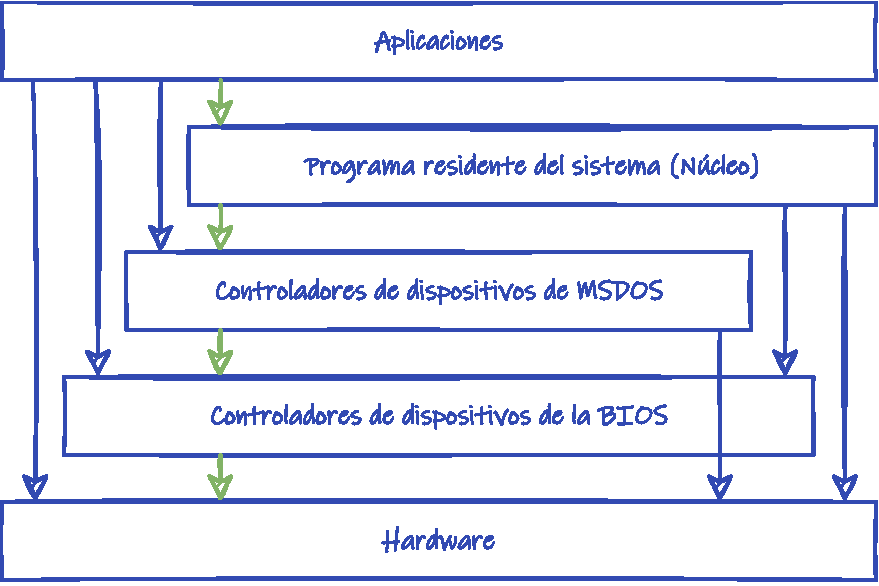
\includegraphics[width=0.8\textwidth]{media/C08_estructura/estructura_msdos.pdf}
\caption{Esquema de la estructura de
MS-DOS.}\label{fig-estructura-msdos}
\end{figure}

Como el \{intel8086\} para el que fue escrito MS-DOS no proporcionaba un
modo dual de operación, los diseñadores del sistema no podían evitar que
los programas de usuario accedieran directamente al hardware ni tenían
forma de proteger las distintas partes del sistema operativo.

\subsection{UNIX}\label{_unix}

Otro ejemplo es el de \href{https://es.wikipedia.org/wiki/Unix}{UNIX
original}, donde sí había una separación clara entre procesos de usuario
y código del sistema, pero juntaba mucha funcionalidad en el núcleo del
sistema.

\begin{figure}
\centering
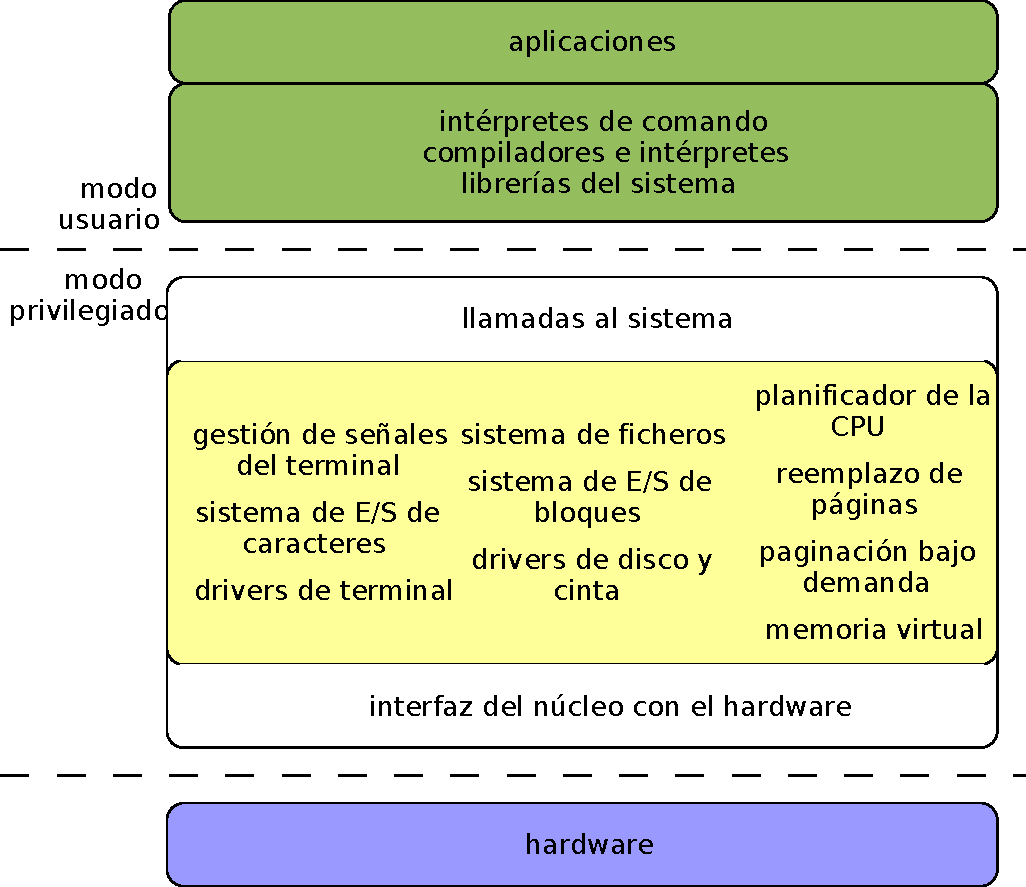
\includegraphics[width=0.8\textwidth]{media/C08_estructura/estructura_unix.pdf}
\caption{Esquema de la estructura de UNIX.}\label{fig-estructura-unix}
\end{figure}

El núcleo proporciona la planificación de CPU, la gestión de la memoria,
el soporte de los sistemas de archivos y muchas otras funcionalidades
del sistema operativo. En general se trata de una enorme cantidad de
funcionalidad que es difícil de implementar y mantener, si no se
compartimenta adecuadamente.

Tanto MS-DOS como UNIX eran originalmente sistemas pequeños y simples,
limitados por las funcionalidades del hardware de su época, que fueron
creciendo más allá de las previsiones originales. Lo cierto es que con
mejor soporte del hardware se puede dividir el sistema operativo en
piezas más pequeñas y apropiadas que las del MS-DOS y el UNIX original.

\section{Estructura en capas}\label{_estructura_en_capas}

{} Los sistemas con \textbf{estructura en capas} se caracterizan por:

\begin{itemize}
\item
  La funcionalidad se divide en capas, de tal forma que una capa solo
  utiliza funciones y servicios de la capa inmediatamente inferior y lo
  hace a través de una interfaz bien definida.
\item
  Como en la programación orientada a objetos, cada capa oculta a la
  capa superior los detalles de su implementación. Por ejemplo, las
  estructuras de datos internas que usa y las operaciones o el hardware
  de la capa inferior que utiliza.
\item
  Escalan mejor que los sistemas con \textbf{estructura sencilla} porque
  las capas hacen que el código esté mejor compartimentado. Por ejemplo,
  al corregir un \emph{bug} o añadir una nueva funcionalidad solo hay
  que preocuparse de su efecto en la capa a la que afecta y no en todo
  el código del núcleo ---siempre que no se altere la interfaz de la
  capa con el exterior---.
\item
  Ser menos eficiente que la de los sistemas de \textbf{estructura
  sencilla}. En cada capa los argumentos son transformados y los datos
  necesarios deben de ser transferidos al invocar operaciones en la capa
  inferior, por lo que cada una añade cierto nivel de sobrecarga al
  funcionamiento del sistema.
\item
  También son sistemas \textbf{monolíticos}, dado que gran parte de la
  funcionalidad del sistema se implementa en el núcleo, aunque ahora el
  núcleo esté compartimentado en capas.
\end{itemize}

Actualmente, no existe ningún motivo para diseñar sistemas operativos
con esta estructura. Es preferible utilizar la \textbf{estructura
modular}, que presenta las mismas ventajas y evita las dificultades en
el diseño, de las que hablaremos a continuación.

Un ejemplo de este tipo de sistemas operativos es el \{os2\}.

\begin{figure}
\centering
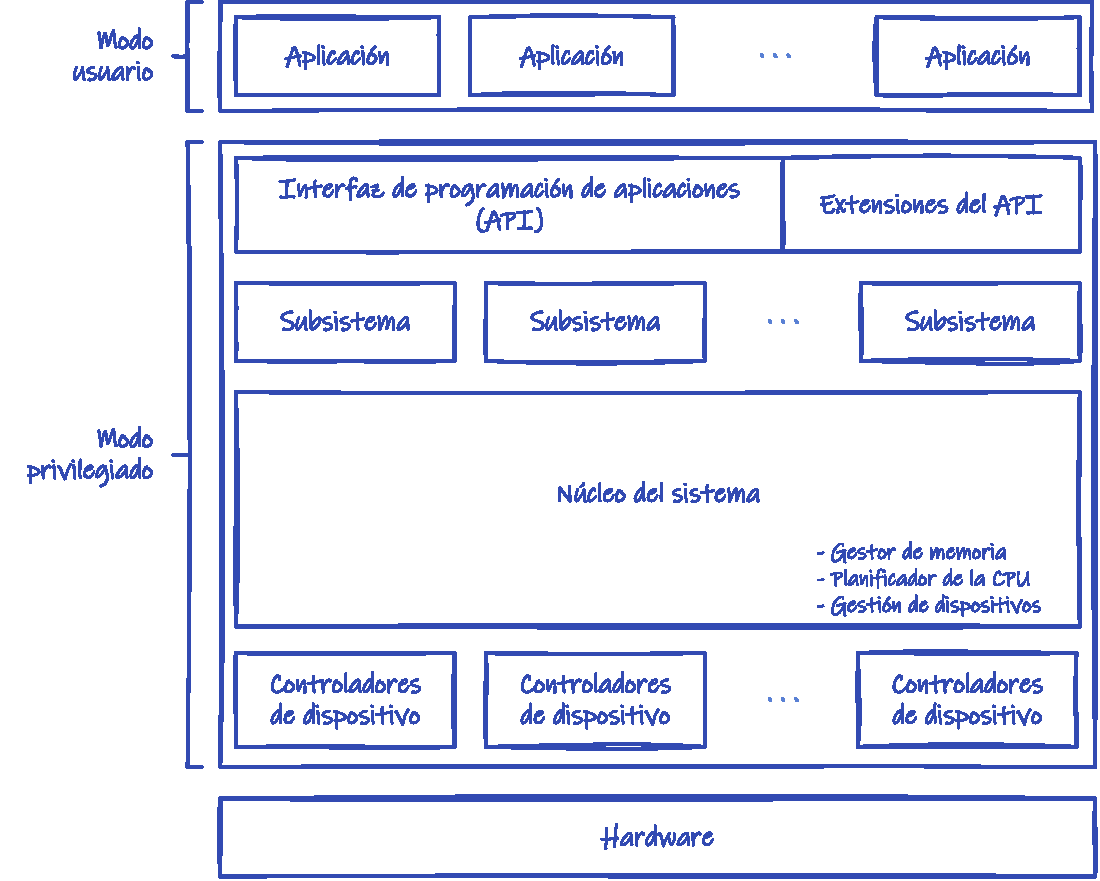
\includegraphics[width=0.8\textwidth]{media/C08_estructura/estructura_os2.pdf}
\caption{Esquema de la estructura de IBM
OS/2.}\label{fig-estructura-os2}
\end{figure}

\subsection{Dificultades con el
diseño}\label{_dificultades_con_el_diseuxf1o}

Es importante tener en cuenta que diseñar un sistema con
\textbf{estructura en capas} no es tan sencillo como pudiera parecer. La
definición de las capas y sus funcionalidades debe ser planificada
cuidadosamente debido a la restricción, comentada anteriormente, de que
una capa solo puede utilizar los servicios de las capas inferiores.

Por ejemplo, el planificador de la CPU suele tener información de los
procesos que están en la memoria. Parte de esa información puede ser
almacenada en el disco para aumentar la memoria principal disponible.
Esto nos debería llevar a pensar que la gestión del almacenamiento
secundario debe ir en una capa inferior a la del planificador de la CPU,
para que así el segundo pueda pedir al primero que guarde los datos en
disco.

Sin embargo, el planificador de la CPU debe asignar la CPU a otro
proceso cuando el proceso que actualmente la ocupa solicita alguna
operación de E/S ---lo típico en multiprogramación---. Como es la
gestión del almacenamiento secundario el que debe pedir una operación al
planificador de la CPU, ahora el primero debe estar sobre el segundo.

La solución a esta dependencia circular es hacer que ambos componentes
estén en la misma capa. Este tipo de dependencias no son raras, ocurre
en muchos otros casos, ya que los componentes del sistema operativo
suelen depender mucho unos de otros.

Al final, la solución de compromiso es tender hacia sistemas con muy
pocas capas donde cada una tiene mucha funcionalidad. Esto limita mucho
las ventajas de esta técnica porque no permite compartimentar el núcleo
tanto como sería deseable.

\section{Microkernel}\label{_microkernel}

{} {} Los sistemas con \textbf{estructura microkernel} se caracterizan
por:

\begin{itemize}
\item
  Eliminar todos los componentes no esenciales del núcleo e
  implementarlos como procesos de usuario.
\item
  Un núcleo \textbf{microkernel} proporciona funciones mínimas de
  gestión de procesos y de memoria y algún mecanismo de comunicación
  entre procesos. Sin embargo, hay que tener en cuenta que hay poco
  consenso a este respecto, por lo que algunos \textbf{microkernel}
  reales incluyen en el núcleo algunas funcionalidades adicionales.
\item
  El mecanismo de comunicación permite a los procesos de los usuarios
  solicitar servicios a los componentes del sistema. También sirve para
  que los componentes del sistema se comuniquen entre sí y se pidan
  servicio.
\end{itemize}

Aunque se puede utilizar en cualquier ámbito, este tipo de estructura se
utiliza, principalmente, en algunos sistemas operativos para sistemas
empotrados, como ocurre con los de \textbf{estructura simple}. Sin
embargo, la \textbf{estructura microkernel} necesita un hardware algo
más potente, que admita modo dual de operación; siendo especialmente
interesante en sistemas críticos o cuando hay especial preocupación por
la seguridad. Algunos ejemplos son los sistemas de automoción o los
equipos médicos.

Dado que los componentes del sistema están aislados unos de otros ---ya
que se implementan como procesos de usuario--- el mecanismo de
comunicación entre procesos es la única forma que tienen los procesos de
los usuarios y los componentes, de solicitarles un servicio.

\begin{figure}
\centering
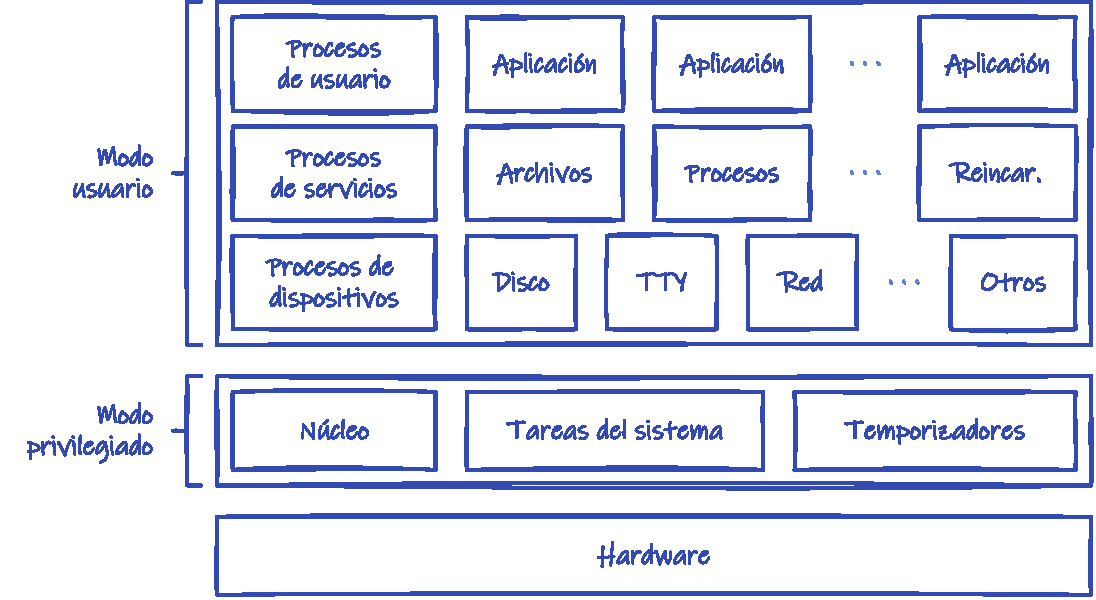
\includegraphics[width=0.8\textwidth]{media/C08_estructura/estructura_minix3.pdf}
\caption{Esquema de la estructura microkernel de MINIX
3.}\label{fig-estructura-minix3}
\end{figure}

Generalmente esta comunicación se implementa mediante paso de mensajes
(véase el \hyperref[_comunicaciuxf3n_entre_procesos]{???}).

Entre los beneficios de estos sistemas operativos se incluyen:

\begin{itemize}
\item
  \textbf{Facilidad a la hora de añadir nuevas funcionalidades}. Los
  nuevos servicios son añadidos como aplicaciones de nivel de usuario,
  por lo que no es necesario hacer modificaciones en el núcleo.
  Desarrollar en el modo privilegiado siempre es más peligrosos que en
  el modo usuario porque los errores pueden ser catastróficos: bloqueo o
  caída del sistema, corrupción de datos, etc.
\item
  \textbf{Facilidad a la hora de llevar el sistema a otras plataformas}.
  Puesto que el núcleo es muy pequeño, resulta muy sencillo de portar a
  otras plataformas.
\item
  \textbf{Más seguridad y fiabilidad}. Puesto que la mayor parte de los
  servicios se ejecutan como procesos separados de usuario, un servicio
  que falla no puede afectar a otros ni puede ser utilizado para ganar
  acceso a otros servicios o al núcleo. Además se pueden implementar
  estrategias para mejorar la tolerancia a fallos, como reiniciar un
  servicio que ha fallado, como si fuera un programa cualquiera.
\end{itemize}

\subsection{Rendimiento}\label{_rendimiento}

El mayor inconveniente es el pobre rendimiento que puede tener, causado
por la sobrecarga que añade el mecanismo de comunicación.

Por ejemplo, \{windowsnt\} nació con una estructura de
\textbf{microkernel} en capas donde una parte importante de los
servicios eran proporcionados por unos procesos de usuario llamados
subsistemas.

El sistema operativo podía mostrar diferentes personalidades o
\emph{entornos operativos} ---básicamente de OS/2, POSIX y MS-DOS--- a
través del uso de subsistemas ambientales, que también se ejecutaban
como procesos de usuario. Las aplicaciones de Microsoft Windows NT se
comunicaban con estos subsistemas utilizando un mecanismo de
comunicación denominado
\href{https://en.wikipedia.org/wiki/Local_Inter-Process_Communication}{LPC}
(\emph{Local Inter-Process Communication}).

Con esta estructura, la pérdida de rendimiento respecto a Microsoft
Windows 95 era tan importante ---especialmente en lo relativo a
operaciones gráficas--- que los diseñadores se vieron obligados a mover
más servicios al espacio del núcleo en la versión 4.0. El resultado es
que los Windows sucesores a Windows NT 4.0 tienen una arquitectura más
monolítica que microkernel, ya que aunque muchos servicios siguen siendo
proporcionados por procesos de usuario, esto solo ocurre con aquellos
donde el rendimiento no es un factor crítico.

Microsoft Windows XP tiene 280 llamadas al sistema a las que hay que
sumar las más de 650 llamadas del subsistema gráfico, que también se
aloja en el núcleo desde Microsoft Windows NT 4.0. Mientras que
Microsoft Windows NT 3.51 tenía algo menos de 200 llamadas al sistema.

Sin embargo, varios sistemas operativos siguen utilizando núcleos
\textbf{microkernel}, como \{qnx\} o \{minix3\}. Ambos son sistemas
operativos de tiempo real, que basan en la estructura de
\textbf{microkernel} su estabilidad como sistema para tareas críticas.

En la \hyperref[fig-estructura-minix3]{Esquema de la estructura
microkernel de MINIX 3.}, por ejemplo, se puede observar un esquema de
\{minix3\}. El núcleo es muy pequeño ---apenas tiene 5000 líneas de
código--- por lo que la mayor parte de la funcionalidad reside en los
procesos de servicios y de controladores de dispositivo.

\{minix3\} es un sistema compatible POSIX. Así que soporta las llamadas
al sistema definidas por este estándar, pero estas se convierten en
mensajes enviados al servidor correspondiente con la petición, y no en
llamadas directas al núcleo. Para que un servidor pueda atender una
petición, quizás tenga que enviar peticiones a otros servidores o
controladores de dispositivo. Incluso pueden tener que hacer llamadas al
núcleo, para solicitar alguna operación privilegiada que no se puede
implementar en el modo usuario. Por ejemplo, operaciones de E/S
---fundamentales para los controladores de dispositivo--- o el acceso a
tablas del núcleo ---como la tabla de procesos---.

Es este trasiego de mensajes con peticiones y respuestas ---y la
correspondiente conmutación de procesos en la CPU para ejecutar el
proceso que atiende cada mensaje--- para resolver una petición de un
proceso de usuario, lo que teóricamente justifica el menor rendimiento
de los sistemas \textbf{microkernel}.

\section{Estructura modular}\label{_estructura_modular}

Los sistemas con \textbf{estructura modular} se caracterizan por:

\begin{itemize}
\item
  Dividir el núcleo en módulos, cada uno de los cuales implementa
  funciones y servicios concretos y se comunican entre sí a través de
  una interfaz bien definida.
\item
  Como en la programación orientada a objetos, cada módulo oculta al
  resto los detalles de su implementación.
\item
  Todos los módulos pueden llamar a funciones de la interfaz de
  cualquier otro módulo, a diferencia de los sistemas operativos con
  \textbf{estructura en capas}, donde una capa solo podía usar a la
  inmediatamente inferior.
\item
  También son sistemas \textbf{monolíticos}, dado que gran parte de la
  funcionalidad del sistema se implementa en el núcleo, aunque ahora el
  núcleo esté compartimentado en módulos.
\end{itemize}

La mayor parte de los sistemas operativos de propósito general, que se
instalan tanto en sistema de escritorio como en servidores, son de este
tipo. También en los \emph{smartphones}, \emph{smart TV} y otros
dispositivos «inteligentes» y, en general, en muchos sistemas
empotrados.

Estos núcleos suelen disponer de un pequeño conjunto de componentes
fundamentales que se cargan durante el arranque. Posteriormente pueden
cargar módulos adicionales, tanto durante la inicialización del sistema
como en tiempo de ejecución.

\begin{figure}
\centering
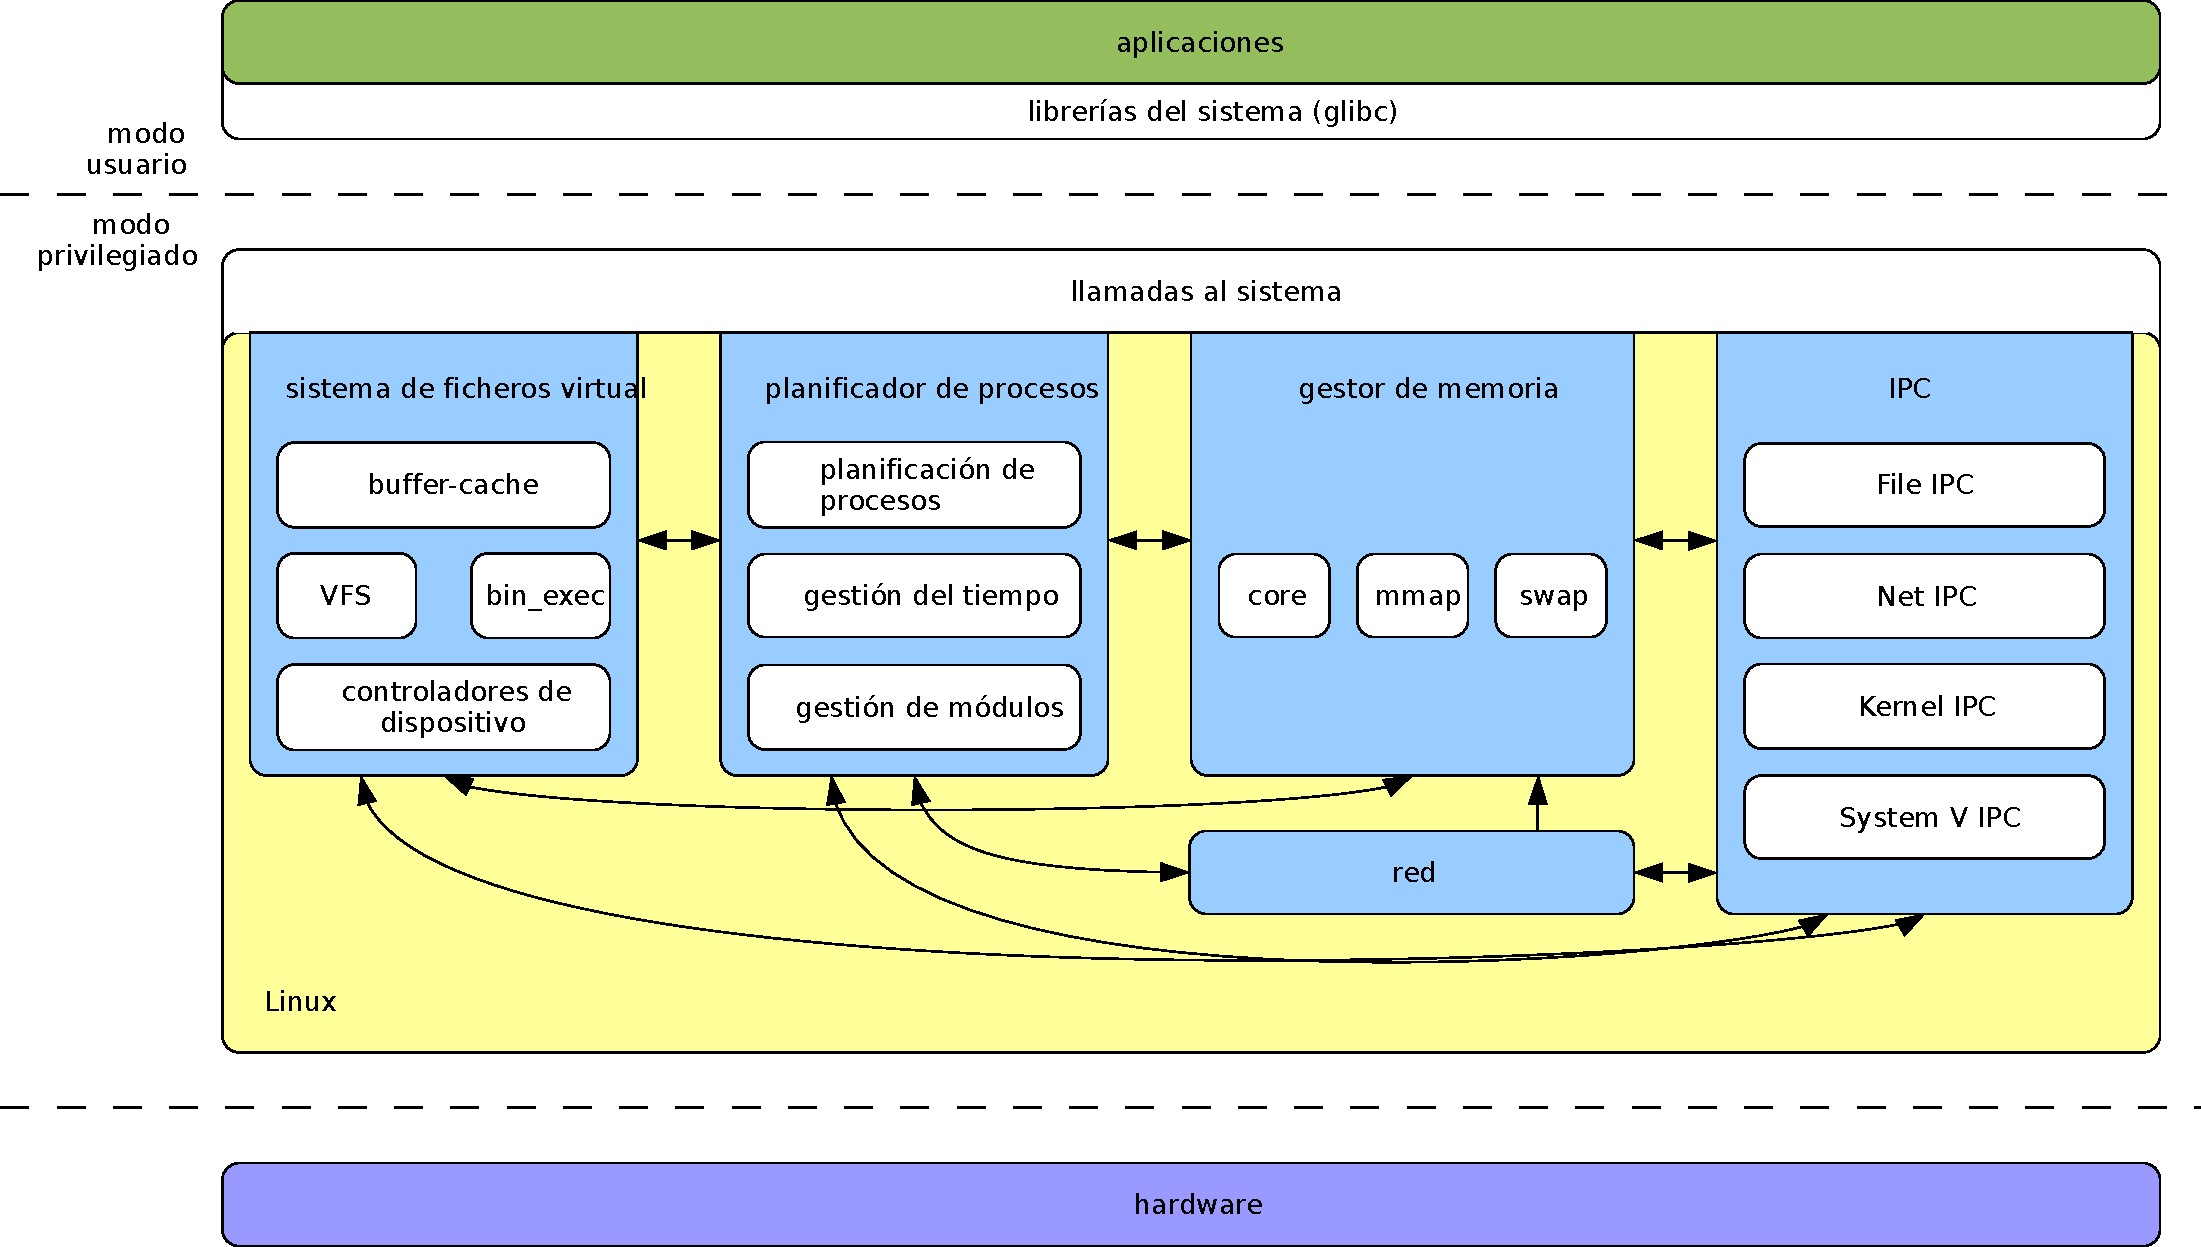
\includegraphics[width=0.8\textwidth]{media/C08_estructura/estructura_linux.pdf}
\caption{Esquema de la estructura del núcleo
Linux.}\label{fig-estructura-linux}
\end{figure}

En este aspecto se asemejan a los núcleos \textbf{microkernel}, ya que
el módulo principal solo tiene funciones básicas. Sin embargo los
núcleos modulares:

\begin{itemize}
\item
  \textbf{Son más eficientes} al no necesitar un mecanismo de
  comunicación, puesto que los componentes se cargan en la memoria
  destinada al núcleo, por lo que pueden llamarse directamente.
\item
  \textbf{Son menos seguros y fiables}, puesto que gran parte de su
  funcionalidad se ofrece desde el modo privilegiado. Un error en
  cualquier componente puede comprometer o hacer caer el sistema.
\end{itemize}

Este tipo de estructura es la utilizada en los UNIX modernos, como
\{solaris\}, \{freebsd\}, \{gnulinux\} (véase la
\hyperref[fig-estructura-linux]{Esquema de la estructura del núcleo
Linux.}) y \{macos\}. También se puede considerar que los sistemas
Windows actuales, tienen estructura modular.


% ── Parte III: Gestión de procesos ───────────────────────
\part{Gesti\'{o}n de procesos}
\input{partes/P03_preambulo}
\section{}

\textbf{Tiempo de lectura:} \{s09-reading-time\}

Los primeros sistemas informáticos solo permitían que un programa se
ejecutase cada vez. Dicho programa tenía control completo sobre el
sistema y acceso a todos los recursos del mismo. Por el contrario, los
sistemas \textbf{multitarea} actuales permiten que múltiples programas
sean cargados y ejecutados concurrentemente.

Obviamente esta evolución implica un control más fino y la
compartimentación de los diversos programas, para que no interfieran
unos con otros. Esto, a su vez, conduce a la aparición de la noción de
\textbf{{}proceso}, que no es sino la unidad de trabajo en un sistema
operativo moderno de tiempo compartido.

Por simplicidad, en este capítulo utilizaremos los términos
\textbf{trabajo} y \textbf{proceso} de forma indistinta. A fin de
cuentas tanto los \textbf{trabajos} en los antiguos \emph{mainframes}
como los \textbf{procesos} en los sistemas modernos son la unidad de
trabajo en sus respectivos sistemas y el origen de toda actividad en la
CPU.

Por último, antes de continuar, es importante señalar que en un sistema
operativo hay varios tipos de procesos:

\begin{itemize}
\item
  \textbf{Procesos del sistema}{}. Ejecutan el código del sistema
  operativo contenido en los \textbf{programas del sistema}, que
  generalmente sirven para hacer tareas del sistema operativo que es
  mejor mantener fuera del núcleo.
\item
  \textbf{Procesos de usuario}{}. Ejecutan el código contenido en los
  \emph{programas de aplicación}.
\end{itemize}

Sin embargo, en lo que resta de capítulo, no estableceremos ninguna
distinción entre ellos. En lo que respecta a la gestión de estos
procesos en el sistema, no hay ninguna diferencia.

\section{El proceso}\label{_el_proceso}

Como ya hemos comentado con anterioridad, un \textbf{{}proceso} es un
programa en ejecución (véase el
\hyperref[sect-componente-gestion-de-procesos]{???} para una
definición más completa). Sin embargo, los procesos no solo están
compuestos por el código del programa, sino que también son importantes
otros elementos:

\begin{description}
\item[Segmento de código{}]
Contiene las instrucciones ejecutables del programa. También es conocido
como segmento \textbf{text}{} o \textbf{.text}.
\item[Segmento de datos{}]
Contiene las variables globales y estáticas del programa que se
inicializan con un valor predefinido. También es conocido como segmento
\textbf{.data}.
\item[Segmento BSS{}]
El segmento BSS ---siglas de \emph{block started by symbol}--- contiene
las variables globales y estáticas del programa inicializadas a 0 o sin
inicialización explícita. Como contiene variables globales sin valor
inicial, en el ejecutable, generalmente, solo se guarda la longitud que
debe tener este segmento en la memoria. También es conocido como
segmento \textbf{.bss}.

En el esquema de la \hyperref[fig-proceso-en-memoria]{Anatomía de un
proceso en memoria.}, este segmento suele ir junto al de datos.
\item[Pila{}]
Contiene datos temporales, como los parámetros y direcciones de retorno
de las funciones y las variables locales.
\item[Montón{}]
Contiene el espacio de la memoria que se asigna dinámicamente durante la
ejecución del proceso. También es conocido como \textbf{{}heap}.
\item[Información sobre el estado actual de ejecución]
Como el \textbf{contador de programa}, los valores de los
\textbf{registros de la CPU}, el \textbf{estado} del proceso y más
(véase el \hyperref[_bloque_de_control_de_proceso]{Bloque de control de
proceso}).
\end{description}

Los \textbf{segmentos de código}, \textbf{datos} y \textbf{BSS} por lo
general son secciones dentro del archivo ejecutable que contiene el
programa. El resto de elementos los crea el sistema operativo al cargar
el programa y crear el proceso.

Como vimos en el \hyperref[sect-componente-gestion-de-procesos]{???}
varios procesos pueden estar asociados al mismo programa, pero no por
eso dejan de ser distintos procesos. Todos tendrán una copia del mismo
segmento de código, pero diferente: contador de programa, valores en los
registros de la CPU, pila, segmento de datos, montón y demas
propiedades.

En la \hyperref[fig-proceso-en-memoria]{Anatomía de un proceso en
memoria.} se puede observar la disposición de algunos de estos elementos
de un proceso en el espacio de usuario en la memoria.

\begin{figure}
\centering
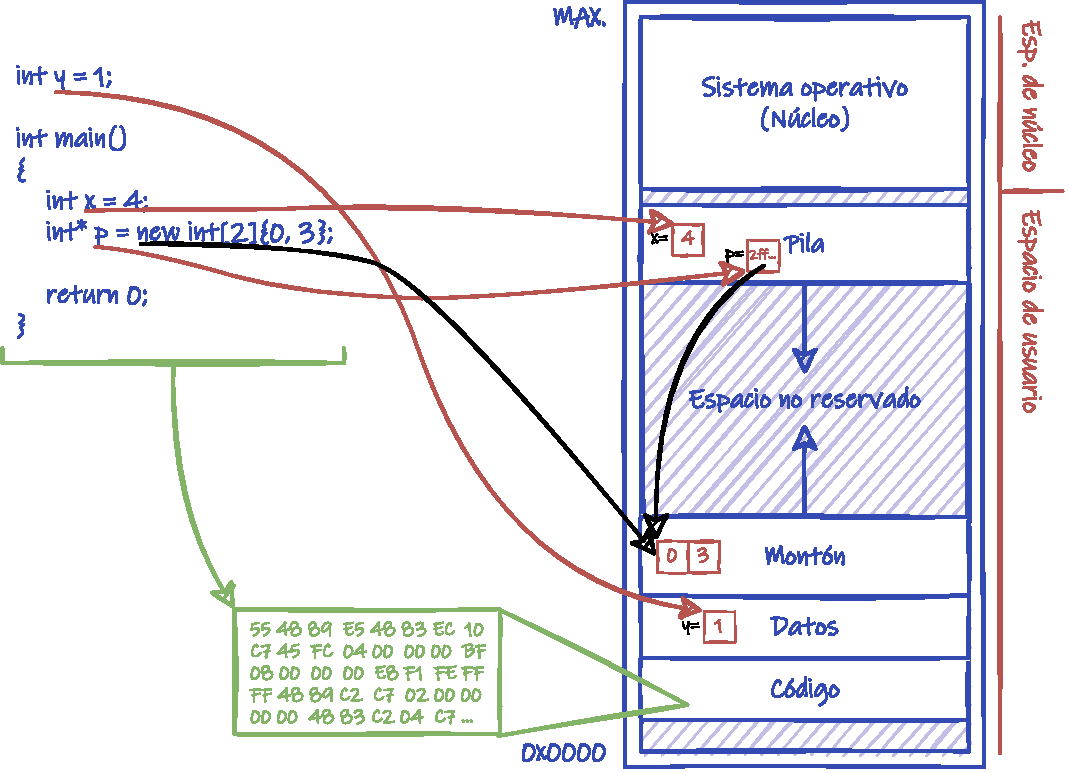
\includegraphics[width=0.8\textwidth]{media/C09_procesos/proceso_en_memoria.pdf}
\caption{Anatomía de un proceso en
memoria.}\label{fig-proceso-en-memoria}
\end{figure}

\section{Estados de los procesos}\label{_estados_de_los_procesos}

Cada proceso tiene un \textbf{estado} que cambia a lo largo de su
ejecución y que está definido, parcialmente, por la actividad que
realiza actualmente el propio proceso.

\begin{figure}
\centering
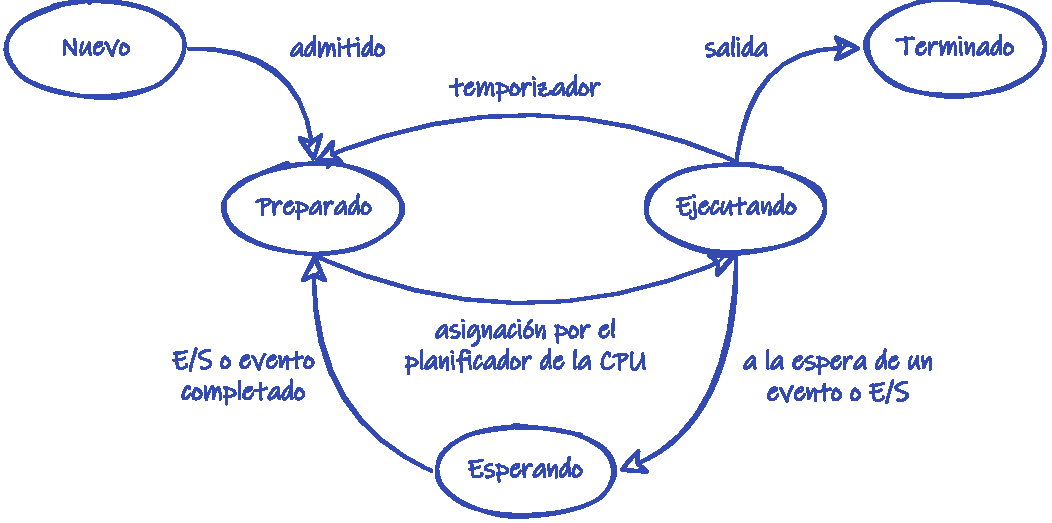
\includegraphics[width=0.8\textwidth]{media/C09_procesos/diagrama_estado_proceso.pdf}
\caption{Diagrama de estado de un
proceso.}\label{fig-diagrama-estado-proceso}
\end{figure}

Los estados por los que puede pasar un proceso varían de un sistema
operativo a otro, aunque los siguientes son comunes a todos ellos:

\begin{description}
\item[Nuevo]
El proceso está en proceso de creación. Este estado existe porque la
creación de un proceso no es algo instantáneo. Necesita de varias
operaciones que pueden tardar tiempo en realizarse, como: reservar
memoria libre, cargar el programa en la memoria, inicializar estructuras
de datos y configurar el entorno de ejecución.
\item[Ejecutando]
El proceso está siendo ejecutado en la CPU. Para eso tiene que haber
sido escogido por el planificador de la CPU de entre todos los procesos
en estado \textbf{preparado}. Solo puede haber un proceso en este estado
por CPU en el sistema.
\item[Esperando]
El proceso está esperando por algún \textbf{evento} como, por ejemplo,
que termine una operación de E/S solicitada previamente o que otro
proceso termine su ejecución. Múltiples procesos pueden estar en este
estado de espera.
\item[Preparado]
El proceso está esperando a poder usar la CPU. Múltiples procesos pueden
estar en este estado.
\item[Terminado]
El proceso ha finalizado su ejecución y espera a que el sistema
operativo recupere los recursos que le fueron asignados. Como en el caso
del estado \textbf{nuevo}, este estado existe porque terminar un proceso
no es algo instantáneo.
\end{description}

El diagrama de estados de los procesos, con las transiciones posibles
entre ellos, se muestra en la
\hyperref[fig-diagrama-estado-proceso]{Diagrama de estado de un
proceso.}.

\section{Bloque de control de
proceso}\label{_bloque_de_control_de_proceso}

{} El \textbf{bloque de control de proceso} o \textbf{{}PCB}
(\emph{Process Control Block}) es una estructura de datos que representa
a cada proceso en el sistema operativo y que guarda información sobre su
estado de actividad actual.

En el sistema hay un PCB por proceso y sirve de almacén para cualquier
información que puede variar de un proceso a otro:

\begin{itemize}
\item
  \textbf{Estado del proceso}. El estado actual del proceso de la lista
  que hemos visto anteriormente. Por ejemplo: nuevo, preparado,
  esperando, etc.
\item
  \textbf{Contador de programa}. Indica la dirección de la próxima
  instrucción del proceso que debe ser ejecutada por la CPU. Obviamente,
  durante el estado \textbf{ejecutando} el contador de programa está en
  el registro correspondiente de la CPU. Su valor se guarda en el PCB al
  salir el proceso de la CPU para que comience ejecutarse en ella otro
  proceso.
\item
  \textbf{Registros de la CPU}. El valor de los registros de la CPU
  también forman parte del estado de actividad del proceso. Como en el
  caso del \textbf{contador de programa}, durante el estado
  \textbf{ejecutando} los valores están en los registros de la CPU, pero
  se guardan en el PCB cuando el proceso sale de la CPU para que se
  ejecute otro proceso.
\item
  \textbf{Información de planificación de la CPU}. Incluye la
  información requerida por el planificador de la CPU. Por ejemplo la
  prioridad del proceso, punteros a las colas de planificación donde
  está el proceso, punteros al PCB del proceso padre y de los procesos
  hijos, etc.
\item
  \textbf{Información de gestión de la memoria}. Incluye la información
  requerida para la gestión de la memoria. Por ejemplo los valores de
  los registros base y límite que definen el área de la memoria física
  que ocupa el proceso ---en el caso de se use asignación contigua de
  memoria (véase el \hyperref[_asignacion_contigua_de_memoria]{???} o
  la dirección a la tabla de páginas ---en el caso de que se use
  paginación (véase el \hyperref[paginacion]{???})---.
\item
  \textbf{Información de registro}. Aquí se incluye la cantidad de CPU
  usada, límites de tiempo en el uso de la CPU, estadísticas de la
  cuenta del usuario a la que pertenece el proceso, estadísticas de la
  ejecución del proceso, etc.
\item
  \textbf{Información de estado de la E/S}. Incluye la lista de
  dispositivos de E/S reservados por el proceso, la lista de archivos
  abiertos, etc.
\end{itemize}

\section{Colas de planificación}\label{_colas_de_planificacion}

{} En los sistemas operativos hay diferentes \textbf{colas de
planificación} para los procesos en distintos \textbf{estados}.

\begin{description}
\item[Cola de trabajo{}]
Contiene todos los trabajos en el sistema, de manera que cuando entran
en el sistema van a esta cola, a la espera de ser escogidos para ser
cargados en la memoria y ejecutados. Esta cola existía en los
\textbf{sistemas multiprogramados}, pero no existe en los
\textbf{sistemas de tiempo compartido} ni en los sistemas operativos
modernos posteriores.
\item[Cola de preparados{}]
Contiene a los procesos que están en estado \textbf{preparado}. Es
decir, procesos cargados en la memoria principal que esperan para usar
la CPU. La cola de preparados es generalmente una lista enlazada de PCB,
donde cada uno incluye un puntero al PCB del siguiente proceso en la
cola.
\item[Colas de espera{}]
Contienen a los procesos que están en estado \textbf{esperando}. Es
decir, que esperan por un evento concreto, como por ejemplo la
finalización de una petición de E/S. Estas colas también suelen ser
implementadas como listas enlazadas de PCB y suele haber una por evento,
de manera que cuando ocurre algún evento todos los procesos en la cola
asociada pasan automáticamente al estado \textbf{preparado} y a la
\textbf{cola de preparados}.
\item[Colas de dispositivo{}]
Son un caso particular de cola de espera. Cada dispositivo de E/S tiene
asociada una \textbf{cola de dispositivo} que contiene los procesos que
están \textbf{esperando} por ese dispositivo en particular.
\end{description}

Una manera habitual de representar la planificación de procesos es a
través de un diagrama de colas como el de la
\hyperref[fig-colas-de-planificacion-procesos]{Diagrama de colas de
la planificación de procesos.}.

\begin{figure}
\centering
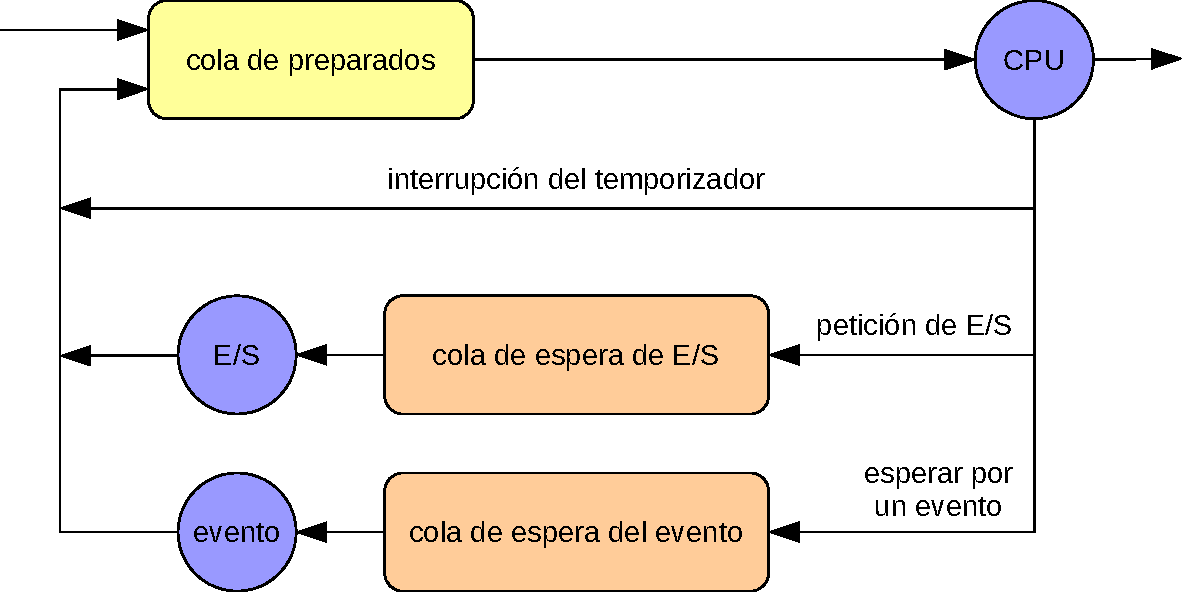
\includegraphics[width=0.8\textwidth]{media/C09_procesos/colas_planificación_procesos.pdf}
\caption{Diagrama de colas de la planificación de
procesos.}\label{fig-colas-de-planificacion-procesos}
\end{figure}

Analizándolo podemos tener una idea clara del flujo típico de los
procesos dentro del sistema:

\begin{enumerate}
\def\labelenumi{\arabic{enumi}.}
\item
  \textbf{Un nuevo proceso llega al sistema}. Una vez pasa del estado
  \textbf{nuevo} a \textbf{preparado} es colocado en la \textbf{cola de
  preparados}. Allí espera hasta que es seleccionado por el
  \textbf{planificado de la CPU} para su ejecución y se le asigna la
  CPU. Mientras se ejecuta pueden ocurrir varias cosas:

  \begin{itemize}
  \item
    \textbf{El proceso solicita una operación de E/S} por lo que
    abandona la CPU y es colocado en la \emph{cola de dispositivo}
    correspondiente en estado \textbf{esperando}. No debemos olvidar que
    aunque en nuestro diagrama no exista más que una de estas colas, en
    un sistema operativo real suele haber una para cada dispositivo.
  \item
    \textbf{El proceso puede querer esperar por un evento}. Por ejemplo,
    puede crear otro proceso y esperar a que termine. En ese caso el
    proceso hijo es creado, mientras el proceso padre abandona la CPU y
    es colocado en una \textbf{cola de espera} en estado
    \textbf{esperando} hasta que el proceso hijo termine. La terminación
    del proceso hijo es el evento que espera el proceso padre para salir
    de la \textbf{cola de espera} y entrar en la \textbf{cola de
    preparados} para continuar su ejecución en la CPU cuando sea
    posible.
  \item
    \textbf{El proceso puede ser sacado forzosamente de la CPU}, como
    resultado de la interrupción del temporizador, que permite
    determinar cuando un proceso lleva demasiado tiempo ejecutándose,
    así que es colocado en la \textbf{cola de preparados} en estado
    \textbf{preparado}.
  \end{itemize}
\item
  \textbf{Cuando las esperas concluyen, los procesos vuelven a la cola
  de preparado}, pasando del estado de espera al de preparado.
\item
  \textbf{Los procesos repiten este ciclo hasta que terminan}. En ese
  momento son eliminados de todas las colas mientras el PCB y los
  recursos asignados son recuperados por parte del sistema operativo
  para poder usarlos con otros procesos.
\end{enumerate}

\section{Planificación de procesos}\label{_planificacion_de_procesos}

Durante su ejecución, los procesos se mueven entre las diversas colas de
planificación a criterio del sistema operativo. Este proceso de
selección debe ser realizado por el \textbf{planificador} adecuado:

\begin{itemize}
\item
  El \textbf{planificador de largo plazo}{} o \textbf{planificador de
  trabajos}{}--- selecciona los trabajos desde la \textbf{cola de
  trabajos} en el almacenamiento secundario ---dónde están todos
  almacenados--- y los carga en memoria.

  Este planificador se usaba en los \textbf{sistemas multiprogramados},
  donde había una \textbf{cola de trabajos}. Los \textbf{sistemas de
  tiempo compartido} posteriores y los sistemas operativos modernos,
  carecen de \textbf{planificador de largo plazo}, porque los programas
  se cargan directamente en memoria para ser ejecutados cuando el
  usuario lo solicita.
\item
  El \textbf{planificador de corto plazo}{} o \textbf{planificador de
  CPU}{} selecciona uno de los procesos en la cola de preparados y lo
  asigna a la CPU. Obviamente este planificador es invocado cuando un
  proceso en ejecución abandona la CPU, dejándola disponible para otro
  proceso.
\item
  El \textbf{planificador de medio plazo} {} era utilizado en algunos
  sistemas para sacar procesos de la memoria cuando escasea y
  reintroducirlos posteriormente cuando vuelve a haber suficiente
  memoria libre. A este esquema se le denomina \textbf{{}intercambio}
  ---o \textbf{\emph{{}swapping}}.

  Esto era útil en sistemas antiguos donde un proceso tenía que estar
  cargado completamente en la memoria para poder ejecutarse. Así que si
  faltaba memoria, se podía suspender un proceso completo, preservar el
  contenido de su memoria en disco y liberar la memoria ocupada para
  usarla con otros procesos.

  En los sistemas de propósito general modernos no se utiliza
  \textbf{planificador de medio plazo} porque utilizan técnicas de
  \textbf{memoria virtual} (véase el \hyperref[memoria_virtual]{???}),
  que permite mover parte de la memoria de los procesos al disco para
  liberar memoria, sin tener que suspender la ejecución del proceso.
\end{itemize}

\section{Cambio de contexto}\label{_cambio_de_contexto}

El \textbf{{}cambio de contexto} es la tarea de asignar la CPU a un
proceso distinto al que la tiene asignada en el momento actual. Esto
implica salvar el estado del viejo proceso en su PCB y cargar en la CPU
el estado del nuevo. Entre la información que debe ser preservada en el
PCB se incluyen:

\begin{itemize}
\item
  El \textbf{contador de programa}.
\item
  Los \textbf{registros de la CPU}.
\item
  El \textbf{estado del proceso}.
\item
  La \textbf{información de gestión de la memoria}. Por ejemplo, la
  información necesaria para configurar el espacio de direcciones del
  proceso.
\end{itemize}

El cambio de contexto es sobrecarga pura, puesto que no hace ningún
trabajo útil mientras se conmuta. Su velocidad depende de aspectos tales
como: el número de registros, la velocidad de la memoria y la existencia
de instrucciones especiales.

Algunas CPU disponen de instrucciones especiales para salvar y cargar
todos los registros de manera eficiente. Esto reduce el tiempo que la
CPU está ocupada en los cambios de contexto.

Otra opción es el uso de
\href{https://en.wikipedia.org/wiki/Register_file}{juegos de registros},
como es el caso de los procesadores \{ultrasparc\} e \{itanium\}. Con
ellos el juego de registros actual de la CPU se mapea sobre un banco de
registros mucho más extenso. Al hacer cambio de contexto, se mapea el
juego de registros a otros registros diferentes del banco. Esto permite
a la CPU almacenar de forma eficiente el valor de los registros de más
de un proceso, sin que en cada cambio de contexto sea necesario
copiarlos al PCB del proceso en la memoria principal.

\section{Operaciones sobre los
procesos}\label{_operaciones_sobre_los_procesos}

En general es necesario que los procesos pueden ser creados y eliminados
dinámicamente, por lo que los sistemas operativos deben proporcionar
servicios para la creación y terminación de los mismos.

\subsection{Creación de procesos}\label{_creacion_de_procesos}

Un proceso ---denominado \textbf{padre}--- puede crear múltiples
procesos ---los \textbf{hijos}--- utilizando una llamada al sistema
específica para la creación de procesos. Cada proceso creado se
identifica de manera unívoca mediante un \textbf{{}identificador de
proceso} o \textbf{{}PID} (\emph{Process Identifier}), que normalmente
es un número entero.

Por ejemplo en sistemas POSIX un programa puede crear otro proceso así:

\begin{Shaded}
\begin{Highlighting}[]
\NormalTok{pid\_t pid }\OperatorTok{=}\NormalTok{ fork}\OperatorTok{();}
\end{Highlighting}
\end{Shaded}

mientras que en Windows API es así:

\begin{Shaded}
\begin{Highlighting}[]
\NormalTok{PROCESS\_INFORMATION pi }\OperatorTok{=} \OperatorTok{\{}\DecValTok{0}\OperatorTok{\};}
\ControlFlowTok{if} \OperatorTok{(}\NormalTok{ CreateProcess}\OperatorTok{(} \StringTok{"C:}\SpecialCharTok{\textbackslash{}\textbackslash{}}\StringTok{Windows}\SpecialCharTok{\textbackslash{}\textbackslash{}}\StringTok{System32}\SpecialCharTok{\textbackslash{}\textbackslash{}}\StringTok{charmap.exe"}\OperatorTok{,} \CommentTok{/* ... */}\OperatorTok{,} \OperatorTok{\&}\NormalTok{pi }\OperatorTok{))} 
\OperatorTok{\{}
\NormalTok{    DWORD pid }\OperatorTok{=}\NormalTok{ pi}\OperatorTok{.}\NormalTok{dwhProcessId}\OperatorTok{;} 
\NormalTok{    HANDLE handle }\OperatorTok{=}\NormalTok{ pi}\OperatorTok{.}\NormalTok{hProcess}\OperatorTok{;} 
\OperatorTok{\}}
\end{Highlighting}
\end{Shaded}

\begin{itemize}
\item
  \{win32\_createprocess\} devuelve \texttt{TRUE} si el proceso se creó
  con éxito.
\item
  \{win32\_processinformation\} contiene el \textbf{identificador de
  proceso} del nuevo proceso, si \{win32\_createprocess\} ha tenido
  éxito.
\item
  \{win32\_processinformation\} también contiene el manejador del
  proceso ---o \emph{handle} en inglés--- que sirve para obtener y
  manipular el nuevo proceso.
\end{itemize}

En ambos casos \texttt{pid} identifica al nuevo proceso en el sistema.
Sin embargo, mientras que los sistemas POSIX ese identificador se puede
usar en otras llamadas al sistema para indicar futuras operaciones sobre
el proceso, en Windows lo que se utiliza es el manejador
\texttt{hProcess} devuelto en \{win32\_processinformation\}.

Obviamente, cada proceso puede obtener del sistema su propio
identificador de procesos:

\begin{Shaded}
\begin{Highlighting}[]
\CommentTok{/* POSIX API */}
\NormalTok{pid\_t pid }\OperatorTok{=}\NormalTok{ getpid}\OperatorTok{();}

\CommentTok{/* Windows API */}
\NormalTok{HANDE handle }\OperatorTok{=}\NormalTok{ GetCurrentProcess}\OperatorTok{();}
\NormalTok{DWORD pid }\OperatorTok{=}\NormalTok{ GetProcessId}\OperatorTok{(}\NormalTok{ handle }\OperatorTok{);}
\end{Highlighting}
\end{Shaded}

o el de su padre:

\begin{Shaded}
\begin{Highlighting}[]
\CommentTok{/* POSIX API */}
\NormalTok{pid\_t parent }\OperatorTok{=}\NormalTok{ getppid}\OperatorTok{();}
\end{Highlighting}
\end{Shaded}

\subsubsection{Árbol de procesos}\label{_uxe1rbol_de_procesos}

Puesto que cada nuevo proceso puede a su vez crear otros procesos, al
final se acaba obteniendo un \textbf{árbol de procesos}. En los sistemas
POSIX es muy sencillo de ver ejecutando el comando \{cmd\_pstree\}.

\begin{figure}
\centering
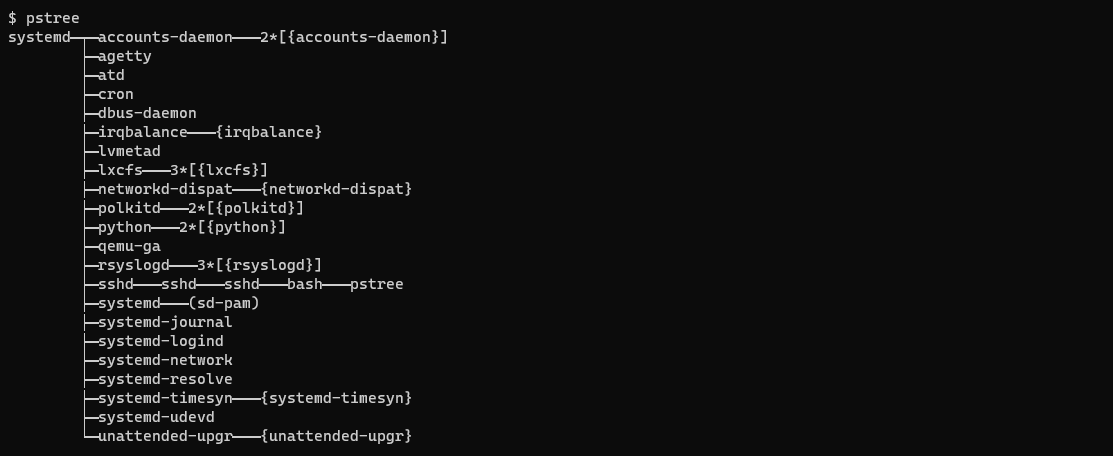
\includegraphics[keepaspectratio]{media/C09_procesos/pstree.png}
\caption{Ejemplo de árbol de procesos mostrador por el comando
pstree.}\label{fig-pstree}
\end{figure}

En estos sistemas se conoce como proceso \textbf{{}init} al proceso
padre raíz de todos los procesos de usuario. Su PID siempre es 1, ya que
es el primer proceso creado por el sistema operativo al terminar la
inicialización del núcleo. Por lo tanto, es el responsable de crear
todos los otros procesos que son necesarios para el funcionamiento del
sistema.

En la \hyperref[fig-pstree]{Ejemplo de árbol de procesos mostrador por
el comando pstree.} se observa que \texttt{systemd} es el proceso
\textbf{{}init}, como ocurre frecuentemente en muchos sistemas Linux
actuales. Anteriormente, lo común es que los sistemas Linux emplearan
una implementación de \textbf{{}init} basada en la de los UNIX System V.

\subsubsection{Cómo obtienen los procesos hijos los recursos que
necesitan}\label{_como_obtienen_los_procesos_hijos_los_recursos_que_necesitan}

Hay varios aspectos en la creación de los procesos que pueden variar de
un sistema operativo a otro. Uno de ellos es cómo obtienen los procesos
hijos los recursos que necesitan para hacer su trabajo.

Fundamentalmente existen dos alternativas:

\begin{enumerate}
\def\labelenumi{\arabic{enumi}.}
\item
  Que cada proceso hijo pueda solicitar y obtener los recursos
  directamente del sistema operativo, compitiendo por los recursos del
  sistema en las mismas condiciones que el resto de procesos en
  ejecución. Esta es la opción más común en los sistemas de propósito
  general actuales, como Microsoft Windows, Android, Linux, macOS, UNIX
  BSD y muchos otros.
\item
  Que los procesos hijo solo puedan aspirar a obtener un subconjunto de
  los recursos de su padre. Esto es interesante en sistemas diseñados
  para ser muy robustos, ya que evita que un proceso pueda sobrecargar
  el sistema creando múltiples procesos que consuman demasiada memoria o
  tiempo de CPU.
\end{enumerate}

En este último caso, el proceso padre puede estar obligado a repartir
sus recursos entre los procesos hijo. O puede que el sistema les permita
compartir algunos de esos recursos ---como memoria o archivos--- con
algunos de sus hijos.

\subsubsection{Cómo pasar parámetros de inicialización a los procesos
hijo}\label{_como_pasar_paruxe1metros_de_inicializacion_a_los_procesos_hijo}

Generalmente, el proceso padre suele disponer de algún mecanismo para
pasar parámetros de inicialización a sus procesos hijo.

\paragraph{Argumentos de línea de
comandos}\label{_argumentos_de_luxednea_de_comandos}

Por ejemplo, en Windows API un proceso puede usar el segundo argumento
de \{win32\_createprocess\} para indicar al proceso hijo opciones y
argumentos de línea de comandos:

\begin{Shaded}
\begin{Highlighting}[]
\NormalTok{HANDLE handle }\OperatorTok{=}\NormalTok{ CreateProcess}\OperatorTok{(}\StringTok{"C:}\SpecialCharTok{\textbackslash{}\textbackslash{}}\StringTok{holamundo.exe"}\OperatorTok{,} \StringTok{"/v /s foo.txt bar.png"}\OperatorTok{,} \CommentTok{/* ... */} \OperatorTok{);}
\end{Highlighting}
\end{Shaded}

Si el proceso hijo está programado en C o C++, podrá acceder a los
argumentos \texttt{/v}, \texttt{/s}, \texttt{foo.txt} y \texttt{bar.png}
a través de los argumentos \texttt{argc} y \texttt{argv} de la función
\{clang\_main\} del programa:

\begin{Shaded}
\begin{Highlighting}[]
\DataTypeTok{int}\NormalTok{ main }\OperatorTok{(}\DataTypeTok{int}\NormalTok{ argc}\OperatorTok{,} \DataTypeTok{char}\OperatorTok{*}\NormalTok{ argv}\OperatorTok{[])}
\OperatorTok{\{}
    \CommentTok{/* . . . */}
\OperatorTok{\}}
\end{Highlighting}
\end{Shaded}

de forma que \texttt{argv{[}0{]}} contendrá \texttt{/v},
\texttt{argv{[}2{]}} contendrá \texttt{/s} y así sucesivamente.

Obviamente, en otros lenguajes de programación se accede de manera
diferente a estos argumentos de línea de comandos.

\paragraph{Variables de entorno}\label{_variables_de_entorno}

Otra forma de pasar parámetros a un proceso hijo es usando las
\textbf{variables de entorno}, que no son sino variables dinámicas que
se pueden crear, leer y modificar durante la ejecución del proceso.

Las \textbf{variables de entorno} se gestionan con funciones específicas
ofrecidas por la API del sistema operativo:

\begin{longtable}[]{@{}
  >{\raggedright\arraybackslash}p{(\linewidth - 4\tabcolsep) * \real{0.3333}}
  >{\raggedright\arraybackslash}p{(\linewidth - 4\tabcolsep) * \real{0.3333}}
  >{\raggedright\arraybackslash}p{(\linewidth - 4\tabcolsep) * \real{0.3333}}@{}}
\caption{Funciones de la API para gestionar variables de
entorno.}\tabularnewline
\toprule\noalign{}
\begin{minipage}[b]{\linewidth}\raggedright
\end{minipage} & \begin{minipage}[b]{\linewidth}\raggedright
POSIX API
\end{minipage} & \begin{minipage}[b]{\linewidth}\raggedright
Windows API
\end{minipage} \\
\midrule\noalign{}
\endfirsthead
\toprule\noalign{}
\begin{minipage}[b]{\linewidth}\raggedright
\end{minipage} & \begin{minipage}[b]{\linewidth}\raggedright
POSIX API
\end{minipage} & \begin{minipage}[b]{\linewidth}\raggedright
Windows API
\end{minipage} \\
\midrule\noalign{}
\endhead
\bottomrule\noalign{}
\endlastfoot
\textbf{Leer} & \{clang\_getenv\} & \{win32\_getenvironmentvariable\} \\
\textbf{Leer todos} & \{clang\_environ\} &
\{win32\_getenvironmentstrings\} \\
\textbf{Crear / modificar} & \{clang\_setenv\} &
\{win32\_setenvironmentvariable\} \\
\end{longtable}

por ejemplo, en sistemas POSIX un programa puede leer la variable de
entorno \texttt{PATH} así:

\begin{Shaded}
\begin{Highlighting}[]
\DataTypeTok{char}\OperatorTok{*}\NormalTok{ path }\OperatorTok{=}\NormalTok{ getenv}\OperatorTok{(}\StringTok{"PATH"}\OperatorTok{);}
\end{Highlighting}
\end{Shaded}

mientras que en Windows API es así:

\begin{Shaded}
\begin{Highlighting}[]
\NormalTok{DWORD buffSize }\OperatorTok{=} \DecValTok{4096}\OperatorTok{;}
\NormalTok{TCHAR path}\OperatorTok{[}\NormalTok{buffSize}\OperatorTok{];}
\NormalTok{GetEnvironmentVariable}\OperatorTok{(}\StringTok{"PATH"}\OperatorTok{,}\NormalTok{ path}\OperatorTok{,}\NormalTok{ buffSize}\OperatorTok{);} 
\end{Highlighting}
\end{Shaded}

\begin{itemize}
\item
  El valor de la variable de entorno \texttt{PATH} se copia en
  \texttt{path}.
\end{itemize}

Usando \{clang\_setenv\} o \{win32\_setenvironmentvariable\} de forma
similar, cualquier proceso puede crear variables de entorno que serán
accesibles a sus procesos hijos, porque por defecto los nuevos procesos
heredan un duplicado de las variables de entorno de su proceso padre.
Así se pueden pasar parámetros de configuración para alterar el
comportamiento de los procesos hijo.

Todas las variantes de sistemas UNIX, así como MS-DOS y todas las
versiones de Microsoft Windows soportan variables de entorno.

\paragraph{Herencia de recursos}\label{_herencia_de_recursos}

En algunos sistemas operativos los procesos hijos pueden heredar cierto
tipo de recursos del proceso padre, lo que también puede servir para
inicializar y alterar el comportamiento del proceso hijo.

Por ejemplo, en los sistemas POSIX todos los archivos abiertos por un
proceso son heredados en el mismo estado por sus hijos. Lo interesante
es que en estos sistemas muchos recursos se gestionan como archivos.
Algunos ejemplos podrían ser: dispositivos de E/S, memoria compartida,
tuberías, \emph{sockets} y otros mecanismos de comunicación.

En POSIX todo proceso tiene, por defecto, tres archivos abiertos que
corresponden a tres dispositivos de E/S especiales:

\begin{itemize}
\item
  \textbf{Entrada estándar}{}, de donde los procesos leen la entrada del
  teclado de la terminal.
\item
  \textbf{Salida estándar}{}, donde el proceso escribe para mostrar
  texto en la pantalla de la terminal.
\item
  \textbf{Salida de error}{}, usada para mostrar errores en la pantalla
  de la terminal.
\end{itemize}

Debido a la herencia de los archivos abiertos del proceso padre, todo
proceso hijo tiene acceso a estos tres mismos dispositivos. Y a su vez
también la tendrán sus hijos y los hijos de estos. De esta manera, todo
proceso tiene acceso a los dispositivos de E/S de la terminal donde se
ejecuta. Pero también permite a un proceso controlar el destino de la
E/S de un proceso hijo ---y de los hijos de este---.

Por ejemplo, si antes de crear el proceso hijo sustituye el dispositivo
de salida estándar por un archivo real, todo lo que el hijo intente
mostrar por pantalla se guardará en dicho archivo, en lugar de
mostrarse. Mientras que si lo hace con el dispositivo de entrada
estándar, todo lo que pretenda leer de teclado realmente lo leerá de un
archivo que el padre puede haber preparado, como si de algún tipo de
control remoto se tratara.

Esta misma idea se puede extender a procesos que ofrecen servicios, ya
sea a otros procesos del mismo sistema o a redes de ordenadores, como
Internet.

Cada conexión con un cliente es como archivo abierto, por lo que los
hijos del proceso heredan las conexiones. Así que es común la estrategia
de crear un hijo por conexión para que la atienda en nombre del padre,
mientras este se encarga de recibir nuevas conexiones.

En Microsoft Windows existe un mecanismo similar pero no por defecto. La
función \{win32\_createprocess\} de Windows API permite indicar si se
quiere que el nuevo proceso herede los recursos abiertos. Y también
tiene ajustes específicos para la entrada y salida estándar y la salida
de error del nuevo proceso.

\subsubsection{Qué ocurre con la ejecución del
padre}\label{_quuxe9_ocurre_con_la_ejecucion_del_padre}

Se suelen contemplar dos posibilidades en términos de la ejecución del
padre:

\begin{enumerate}
\def\labelenumi{\arabic{enumi}.}
\item
  Que el padre continúe ejecutándose al mismo tiempo que el hijo. Es lo
  más común en los sistemas multitarea actuales.
\item
  Que el padre quede detenido a la espera de que algunos o todos sus
  hijos terminen. Era lo más frecuente en sistemas monotarea, como
  \{msdos\}.
\end{enumerate}

\subsubsection{Cómo se construye el espacio de direcciones de los
procesos
hijo}\label{_como_se_construye_el_espacio_de_direcciones_de_los_procesos_hijo}

En general hay dos posibilidades:

\begin{enumerate}
\def\labelenumi{\arabic{enumi}.}
\item
  Que el espacio de direcciones del proceso hijo sea un duplicado del
  que tiene el padre. Es decir, que inicialmente el hijo tenga el mismo
  código y datos que el padre. Es lo que hace \{linux\_fork\} en los
  sistemas POSIX.
\item
  Que el espacio de direcciones del proceso hijo se cree desde cero y se
  cargue en él un nuevo programa. Es lo que hace
  \{win32\_createprocess\} en Windows. Por eso siempre hay que indicarle
  el nombre del programa que se quiere ejecutar en el nuevo proceso.
\end{enumerate}

Esto lo veremos con más detalle en el
\hyperref[_ejemplos_de_operaciones_con_procesos]{Ejemplos de operaciones
con procesos}.

\subsection{Terminación de procesos}\label{_terminacion_de_procesos}

Un proceso termina cuando se lo indica al sistema operativo con la
llamada al sistema \textbf{exit}. En ese momento puede devolver un valor
de estado a su padre.

Esto ocurre en C y C++ incluso si el programa termina usando la
sentencia \texttt{return} en \{clang\_main\}. Lo que ocurre es que es el
código, introducido por el compilador, que llamó a \{clang\_main\} es el
que llama a \textbf{exit} usando el valor devuelto por \{clang\_main\}.

El proceso padre puede esperar a que el hijo termine y recuperar ese
valor a través de la llamada al sistema \textbf{wait}. Cuando un proceso
termina, todos los recursos son liberados, incluyendo: la memoria física
y virtual, archivos y dispositivos abiertos, búferes de E/S, etc.

\begin{longtable}[]{@{}
  >{\raggedright\arraybackslash}p{(\linewidth - 4\tabcolsep) * \real{0.3333}}
  >{\raggedright\arraybackslash}p{(\linewidth - 4\tabcolsep) * \real{0.3333}}
  >{\raggedright\arraybackslash}p{(\linewidth - 4\tabcolsep) * \real{0.3333}}@{}}
\caption{Funciones de la API para salir, esperar y terminar
procesos.}\tabularnewline
\toprule\noalign{}
\begin{minipage}[b]{\linewidth}\raggedright
\end{minipage} & \begin{minipage}[b]{\linewidth}\raggedright
POSIX API
\end{minipage} & \begin{minipage}[b]{\linewidth}\raggedright
Windows API
\end{minipage} \\
\midrule\noalign{}
\endfirsthead
\toprule\noalign{}
\begin{minipage}[b]{\linewidth}\raggedright
\end{minipage} & \begin{minipage}[b]{\linewidth}\raggedright
POSIX API
\end{minipage} & \begin{minipage}[b]{\linewidth}\raggedright
Windows API
\end{minipage} \\
\midrule\noalign{}
\endhead
\bottomrule\noalign{}
\endlastfoot
\textbf{Salir} & \{clang\_exit\} & \{win32\_exitprocess\} \\
\textbf{Esperar (un hijo concreto)} & \{linux\_waitpid\} &
\{win32\_waitforsingleobject\} \\
\textbf{Esperar (múltiples hijos)} & \{linux\_wait\} &
\{win32\_waitformultipleobjects\} \\
\textbf{Terminar otro proceso} & \{linux\_kill\} &
\{win32\_terminateprocess\} \\
\end{longtable}

En todo caso un proceso puede provocar la terminación de otro proceso a
través de una llamada al sistema. Por ejemplo, en sistemas POSIX se usa
un mecanismo llamado \textbf{señales}{}:

\begin{Shaded}
\begin{Highlighting}[]
\NormalTok{kill}\OperatorTok{(}\NormalTok{pid}\OperatorTok{,}\NormalTok{ SIGTERM}\OperatorTok{);}
\end{Highlighting}
\end{Shaded}

mientras que en Windows API:

\begin{Shaded}
\begin{Highlighting}[]
\NormalTok{TerminateProcess}\OperatorTok{(}\NormalTok{handle}\OperatorTok{);}
\end{Highlighting}
\end{Shaded}

Habitualmente el proceso que invoca estas funciones es el proceso padre,
ya que puede que sea el único con permisos para hacerlo.

Los motivos para terminar un proceso hijo pueden ser:

\begin{itemize}
\item
  \textbf{El hijo ha excedido el uso de algunos de los recursos
  reservados}. Obviamente esto tiene sentido cuando los hijos utilizan
  un subconjunto de los recursos asignados al padre.
\item
  \textbf{La tarea asignada al hijo ya no es necesaria}. Por ejemplo, se
  creó para comprimir un archivo, pero el usuario ha pedido cancelar la
  operación.
\item
  \textbf{El padre termina y el sistema operativo está diseñado para no
  permitir que el hijo pueda seguir ejecutándose si no tiene un padre}.
  En esos sistemas, la terminación de un proceso provoca que el sistema
  operativo inicie lo que se denomina una \textbf{{}terminación en
  cascada}, en la que termina todos los procesos que cuelgan de dicho
  proceso.
\end{itemize}

En sistemas UNIX y estilo UNIX, si un proceso muere a sus hijos no
terminan sino que se les reasigna como padre el proceso \textbf{init}.

\subsection{Ejemplos de operaciones con
procesos}\label{_ejemplos_de_operaciones_con_procesos}

En C estándar la función \{clang\_system\} de la librería estándar
permite ejecutar otro proceso, con sus argumentos, esperar a que termine
y obtener el valor de estado con el que finalizó el proceso.

\begin{Shaded}
\begin{Highlighting}[]
\DataTypeTok{int}\NormalTok{ status }\OperatorTok{=}\NormalTok{ system}\OperatorTok{(}\StringTok{"holamundo {-}v foo.txt"}\OperatorTok{);}
\end{Highlighting}
\end{Shaded}

Esta función es portable. Está disponible en cualquier sistema donde
haya un compilador de C estándar, pero sus funcionalidades son bastante
limitadas. Por ejemplo, no permite que el programa padre continúe su
ejecución mientras se ejecuta el hijo, aunque el sistema sea multitarea
y ese sea el comportamiento por defecto. Tampoco facilita el control de
los recursos que son heredados por el proceso hijo o hacer redirecciones
de los dispositivos de E/S estándar.

Como hemos comentado anteriormente, para acceder a todas las
funcionalidades ofrecidas por los sistemas operativos, muchas veces es
necesario utilizar directamente la librería del sistema.

\subsubsection{Windows API}\label{_windows_api}

En Windows la librería del sistema ofrece la función
\{win32\_createprocess\}. A diferencia de \{clang\_system\}, recibe
muchísimos argumentos, ya que permite configurar bastantes aspectos de
la creación de un nuevo proceso.

En el \hyperref[ejemplo-createprocess]{example\_title} se puede ver cómo
se usa \{win32\_createprocess\} para ejecutar un programa y esperar a
que termine, de forma similar a como lo hace \{clang\_system\}.

El código fuente completo de este ejemplo está disponible en
\{createprocess\_cpp\}.

\begin{Shaded}
\begin{Highlighting}[]
\NormalTok{STARTUPINFO si }\OperatorTok{=} \OperatorTok{\{} \KeywordTok{sizeof}\OperatorTok{(}\NormalTok{STARTUPINFO}\OperatorTok{)} \OperatorTok{\};} 
\NormalTok{PROCESS\_INFORMATION pi }\OperatorTok{=} \OperatorTok{\{}\DecValTok{0}\OperatorTok{\};} 

\CommentTok{// Crear procesos hijo y comprobar si no se creó con éxito.}
\ControlFlowTok{if}\OperatorTok{(} \OperatorTok{!}\NormalTok{ CreateProcess}\OperatorTok{(} 
\NormalTok{    NULL}\OperatorTok{,} 
    \StringTok{"C:}\SpecialCharTok{\textbackslash{}\textbackslash{}}\StringTok{Windows}\SpecialCharTok{\textbackslash{}\textbackslash{}}\StringTok{System32}\SpecialCharTok{\textbackslash{}\textbackslash{}}\StringTok{charmap.exe"}\OperatorTok{,}  
\NormalTok{    NULL}\OperatorTok{,}
\NormalTok{    NULL}\OperatorTok{,}
\NormalTok{    FALSE}\OperatorTok{,} 
    \DecValTok{0}\OperatorTok{,}
\NormalTok{    NULL}\OperatorTok{,}  
\NormalTok{    NULL}\OperatorTok{,}  
    \OperatorTok{\&}\NormalTok{si}\OperatorTok{,}
    \OperatorTok{\&}\NormalTok{pi }\OperatorTok{))}
\OperatorTok{\{}
\NormalTok{    fprintf}\OperatorTok{(}\NormalTok{ stderr}\OperatorTok{,} \StringTok{"Error (}\SpecialCharTok{\%d}\StringTok{) al crear el proceso.}\SpecialCharTok{\textbackslash{}n}\StringTok{"}\OperatorTok{,}\NormalTok{ GetLastError}\OperatorTok{()} \OperatorTok{);} 
    \ControlFlowTok{return}\NormalTok{ EXIT\_FAILURE}\OperatorTok{;}
\OperatorTok{\}}

\NormalTok{printf}\OperatorTok{(} \StringTok{"[PADRE] El PID del nuevo proceso hijo es: }\SpecialCharTok{\%d\textbackslash{}n}\StringTok{"}\OperatorTok{,}\NormalTok{ pi}\OperatorTok{.}\NormalTok{dwProcessId }\OperatorTok{);}

\CommentTok{// Esperar hasta que el hijo termine.}
\NormalTok{WaitForSingleObject}\OperatorTok{(}\NormalTok{ pi}\OperatorTok{.}\NormalTok{hProcess}\OperatorTok{,}\NormalTok{ INFINITE }\OperatorTok{);} 

\NormalTok{DWORD dwExitCode}\OperatorTok{;}
\NormalTok{GetExitCodeProcess}\OperatorTok{(}\NormalTok{ pi}\OperatorTok{.}\NormalTok{hProcess}\OperatorTok{,} \OperatorTok{\&}\NormalTok{dwExitCode }\OperatorTok{);} 
\NormalTok{printf}\OperatorTok{(} \StringTok{"[PADRE] El valor de salida del proceso hijo es: }\SpecialCharTok{\%d\textbackslash{}n}\StringTok{"}\OperatorTok{,}\NormalTok{ dwExitCode }\OperatorTok{);}

\CommentTok{// Cerrar los manejadores del proceso y del hilo principal del proceso.}
\NormalTok{CloseHandle}\OperatorTok{(}\NormalTok{ pi}\OperatorTok{.}\NormalTok{hProcess }\OperatorTok{);} 
\NormalTok{CloseHandle}\OperatorTok{(}\NormalTok{ pi}\OperatorTok{.}\NormalTok{hThread }\OperatorTok{);}
\end{Highlighting}
\end{Shaded}

\begin{itemize}
\item
  \{win32\_startupinfo\} sirve para pasar a \{win32\_createprocess\}
  parámetros adicionales sobre el inicio de la aplicación, como
  configurar la redirección de la E/S estándar o características de la
  primera ventana creada por la aplicación ---en aplicaciones con
  interfaz gráfica---. Si no se va a usar, debe inicializarse a 0,
  excepto el primer campo que debe contener el tamaño de la estructura.
\item
  \{win32\_processinformation\} sirve para devolver el manejador y el
  \textbf{identificador de proceso} del nuevo proceso. Es común
  inicializar la estructura a 0.
\item
  \{win32\_createprocess\} devuelve \texttt{TRUE} o \texttt{FALSE}, en
  función de si ha tenido éxito o no, respectivamente.
\item
  El primer argumento ---\texttt{lpApplicationName}--- se usa para pasar
  la ruta del ejecutable, mientras que los argumentos de línea de
  comando generalmente se pasan por el segundo
  ---\texttt{lpCommandLine}---. Si en \texttt{lpApplicationName} se
  indica NULL, se puede pasar todo junto por \texttt{lpCommandLine}.
\item
  En \texttt{lpCommandLine} indicamos la ruta al ejecutable y los
  argumentos de la línea de comandos, si hicieran falta.
\item
  Con \texttt{bInheritHandles} a \texttt{FALSE} señalamos que no
  queremos que el proceso hijo herede ningún manejador abierto del
  proceso padre. Estos manejadores son recursos a los que el padre tiene
  acceso y, si fuera necesario, el hijo también podría tenerlo. Los
  manejadores pueden representar, por ejemplo, archivos abiertos,
  tuberías, \emph{sockets} u otros mecanismos de comunicación, procesos
  o archivos mapeados en memoria, entre muchos otros tipos de recursos.
\item
  Con \texttt{NULL} en \texttt{lpEnvironment} indicamos que el hijo
  herede el conjunto de variables de entorno directamente del padre. La
  otra opción es indicar un nuevo conjunto de variables de entorno.
\item
  \texttt{lpCurrentDirectory} sirve para indicar el directorio del
  trabajo del proceso hijo. Es decir, el directorio respecto al que se
  resolverán las rutas de archivo relativas. Con \texttt{NULL} indicamos
  que utilice la misma ruta que el proceso padre.
\item
  Si \{win32\_createprocess\} falla, devuelve \texttt{FALSE}. Llamando a
  \{win32\_getlasterror\} obtiene el código que identifica el motivo del
  error de la última función utilizada de Windows API.
\item
  Usando \{win32\_waitforsingleobject\} hacemos que el proceso padre se
  quede en estado \textbf{esperando} ---sin que pueda seguir
  ejecutándose--- hasta que el proceso hijo termine.
\item
  Cuando el proceso ha terminado, el padre puede conocer su valor de
  salida. Es decir, el valor usado para terminar en la sentencia
  \texttt{return} de \{clang\_main\} o al llamar a
  \{win32\_exitprocess\} en el programa del proceso hijo. Como
  convención, el hijo indica con un 0 que terminó con éxito, mientras
  que con un valor distinto indica que tuvo algún tipo de problema.
\item
  Cuando ya no hace falta obtener información del proceso hijo o
  manipularlo, es necesario cerrar los manejadores devueltos por
  \{win32\_createprocess\}. Así el sistema operativo sabe que las
  estructuras de datos relacionadas con el proceso hijo ya no son
  necesarias, por lo que pueden liberarse.
\end{itemize}

\{win32\_createprocess\} siempre necesita la ruta a un ejecutable ---sea
en el primer o en el segundo argumento de la función--- porque se
utiliza para crear un proceso completamente limpio y ejecutar en él un
nuevo programa.

\subsubsection{POSIX API}\label{sect-procesos-posix-api}

Por el contrario, en los sistemas POSIX se utiliza una estrategia muy
diferente. Los nuevos procesos se crean con la llamada \{linux\_fork\},
que se encarga de crearlo como una copia del proceso padre.

El código fuente completo de este ejemplo está disponible en
\{fork\_cpp\}.

\begin{Shaded}
\begin{Highlighting}[]
\NormalTok{pid\_t pid }\OperatorTok{=}\NormalTok{ getpid}\OperatorTok{();} 

\CommentTok{// Crear un proceso hijo}
\NormalTok{pid\_t child }\OperatorTok{=}\NormalTok{ fork}\OperatorTok{();} 

\ControlFlowTok{if} \OperatorTok{(}\NormalTok{child }\OperatorTok{==} \DecValTok{0}\OperatorTok{)} 
\OperatorTok{\{}
    \CommentTok{// Aquí solo entra el proceso hijo}
\NormalTok{    puts}\OperatorTok{(} \StringTok{"[HIJO] ¡Soy el proceso hijo!"} \OperatorTok{);}
\NormalTok{    printf}\OperatorTok{(} \StringTok{"[HIJO] El valor de mi variable \textquotesingle{}child\textquotesingle{} es: }\SpecialCharTok{\%d\textbackslash{}n}\StringTok{"}\OperatorTok{,}\NormalTok{ child }\OperatorTok{);} 
\NormalTok{    printf}\OperatorTok{(} \StringTok{"[HIJO] Este es mi PID: }\SpecialCharTok{\%d\textbackslash{}n}\StringTok{"}\OperatorTok{,}\NormalTok{ getpid}\OperatorTok{()} \OperatorTok{);} 
\NormalTok{    printf}\OperatorTok{(} \StringTok{"[HIJO] El valor de mi variable \textquotesingle{}pid\textquotesingle{} es: }\SpecialCharTok{\%d\textbackslash{}n}\StringTok{"}\OperatorTok{,}\NormalTok{ pid }\OperatorTok{);} 
\NormalTok{    printf}\OperatorTok{(} \StringTok{"[HIJO] El PID de mi padre es: }\SpecialCharTok{\%d\textbackslash{}n}\StringTok{"}\OperatorTok{,}\NormalTok{ getppid}\OperatorTok{()} \OperatorTok{);} 

\NormalTok{    puts}\OperatorTok{(} \StringTok{"[HIJO] Durmiendo 10 segundos..."} \OperatorTok{);}
\NormalTok{    sleep}\OperatorTok{(}\DecValTok{10}\OperatorTok{);}

    \DataTypeTok{int}\NormalTok{ status }\OperatorTok{=} \DecValTok{42}\OperatorTok{;}
\NormalTok{    printf}\OperatorTok{(} \StringTok{"[HIJO] Salgo con }\SpecialCharTok{\%d}\StringTok{ ¡Adios!}\SpecialCharTok{\textbackslash{}n}\StringTok{"}\OperatorTok{,}\NormalTok{ status }\OperatorTok{);}
    \ControlFlowTok{return}\NormalTok{ status}\OperatorTok{;} 
\OperatorTok{\}}
\ControlFlowTok{else} \ControlFlowTok{if} \OperatorTok{(}\NormalTok{child }\OperatorTok{\textgreater{}} \DecValTok{0}\OperatorTok{)}  
\OperatorTok{\{}
    \CommentTok{// Aquí solo entra el proceso padre}
\NormalTok{    puts}\OperatorTok{(} \StringTok{"[PADRE] ¡Soy el proceso padre!"} \OperatorTok{);}
\NormalTok{    printf}\OperatorTok{(} \StringTok{"[PADRE] El valor de mi variable \textquotesingle{}child\textquotesingle{} es: }\SpecialCharTok{\%d\textbackslash{}n}\StringTok{"}\OperatorTok{,}\NormalTok{ child }\OperatorTok{);}  
\NormalTok{    printf}\OperatorTok{(} \StringTok{"[PADRE] Este es mi PID: }\SpecialCharTok{\%d\textbackslash{}n}\StringTok{"}\OperatorTok{,}\NormalTok{ getpid}\OperatorTok{()} \OperatorTok{);} 
\NormalTok{    printf}\OperatorTok{(} \StringTok{"[PADRE] El valor de mi variable \textquotesingle{}pid\textquotesingle{} es: }\SpecialCharTok{\%d\textbackslash{}n}\StringTok{"}\OperatorTok{,}\NormalTok{ pid }\OperatorTok{);} 
\NormalTok{    printf}\OperatorTok{(} \StringTok{"[PADRE] El PID de mi padre es: }\SpecialCharTok{\%d\textbackslash{}n}\StringTok{"}\OperatorTok{,}\NormalTok{ getppid}\OperatorTok{()} \OperatorTok{);}

\NormalTok{    puts}\OperatorTok{(} \StringTok{"[PADRE] Voy a esperar a que mi hijo termine..."} \OperatorTok{);}

    \DataTypeTok{int}\NormalTok{ status}\OperatorTok{;}
\NormalTok{    wait}\OperatorTok{(} \OperatorTok{\&}\NormalTok{status }\OperatorTok{);}  
\NormalTok{    printf}\OperatorTok{(} \StringTok{"[PADRE] El valor de salida de mi hijo fue: }\SpecialCharTok{\%d\textbackslash{}n}\StringTok{"}\OperatorTok{,}
\NormalTok{        WEXITSTATUS}\OperatorTok{(}\NormalTok{status}\OperatorTok{)} \OperatorTok{);} 

\NormalTok{    puts}\OperatorTok{(} \StringTok{"[PADRE] ¡Adios!"} \OperatorTok{);}
    \ControlFlowTok{return}\NormalTok{ EXIT\_SUCCESS}\OperatorTok{;}
\OperatorTok{\}}
\ControlFlowTok{else} \OperatorTok{\{} 
    \CommentTok{// Aquí solo entra el padre si no pudo crear el hijo}
\NormalTok{    fprintf}\OperatorTok{(}\NormalTok{ stderr}\OperatorTok{,} \StringTok{"Error (}\SpecialCharTok{\%d}\StringTok{) al crear el proceso: }\SpecialCharTok{\%s\textbackslash{}n}\StringTok{"}\OperatorTok{,}
\NormalTok{        errno}\OperatorTok{,}\NormalTok{ strerror}\OperatorTok{(}\NormalTok{errno}\OperatorTok{)} \OperatorTok{);} 
    \ControlFlowTok{return}\NormalTok{ EXIT\_FAILURE}\OperatorTok{;}
\OperatorTok{\}}
\end{Highlighting}
\end{Shaded}

\begin{itemize}
\item
  El proceso llama a \{linux\_fork\} pero al retornar de la llamada
  vuelven dos procesos: el proceso padre, que es el que llamó
  originalmente a \{linux\_fork\}, y el proceso hijo. Como el proceso
  hijo es una copia del padre, tiene el mismo código, las mismas
  variables y los mismos recursos que tenía el padre en el momento de
  llamar a \{linux\_fork\}. La única diferencia es el valor devuelto por
  \{linux\_fork\}, que guardamos en \texttt{child}.
\item
  Los dos procesos ejecutan el mismo programa, así que ambos llegan a la
  línea detrás del \{linux\_fork\}. Como queremos que cada proceso haga
  cosas diferentes, necesitamos que cada uno vaya a ramas distintas del
  código. Eso se hace comprobando el valor de \texttt{child}, porque si
  vale 0 es que el proceso que actualmente ejecuta el programa es el
  hijo.
\item
  Si, por el contrario, el valor de \texttt{child} es mayor de 0, el
  proceso que ejecuta el programa es el padre y el valor de
  \texttt{child} es el PID del proceso hijo creado.
\item
  Así que el valor de \texttt{child} en el padre coincide con el
  devuelto por \{linux\_getpid\} en el hijo.
\item
  Finalmente, si el valor devuelto por \{linux\_fork\} es negativo, es
  que ocurrió un error y el proceso hijo no llegó a crearse.
\item
  En los sistemas POSIX es común que las llamadas al sistema devuelvan
  un valor negativo para indicar un error. El motivo del error se puede
  conocer a través de la variable global \{linux\_errno\}, que siempre
  guarda el código de identificación del error en la última función
  invocada de la API POSIX. La función \{linux\_strerror\} permite
  obtener un texto descriptivo de cualquier valor de \{linux\_errno\},
  lo que siempre resulta útil para crear mensajes de error que ayuden a
  determinar dónde estuvo el problema.
\item
  A modo de ejemplo hemos guardado el PID del proceso en la variable
  \texttt{pid}, antes de la llamada a \{linux\_fork\}. Como el proceso
  hijo es una copia del proceso padre, la variable existe en ambos, pero
  en el proceso hijo su valor coincide con lo devuelto por
  \{linux\_getppid\} mientras que en el proceso padre con lo devuelto
  por \{linux\_getpid\}.
\item
  \{linux\_wait\} hace que el proceso padre interrumpa su ejecución
  hasta que algún hijo termine y devuelve el estado de salida en
  \texttt{status}.

  Debemos asegurarnos de llamar a \{linux\_wait\} o \{linux\_waitpid\}
  una vez por cada proceso hijo, en algún momento, porque así es como el
  sistema sabe que el padre ya no tiene más interés en el proceso y
  puede liberar su PCB, donde se guarda el estado de salida. No hacerlo
  genera \textbf{procesos zombi}{} o \emph{defunct}.
\item
  El valor de salida del proceso hijo lo obtiene el proceso padre a
  través del estado de salida devuelto por \{linux\_wait\}. Pero ese
  estado contiene más información sobre la causa por la que el proceso
  terminó. Para recuperar el valor de salida se usa la macro
  \texttt{WEXITSTATUS} sobre el estado de salida.
\end{itemize}

Lo siguiente es un posible resultado de ejecutar el programa anterior en
una terminal de Linux, numerado con las anotaciones realizadas al
código:

\begin{verbatim}
$ ./fork
[PADRE] ¡Soy el proceso padre!
[PADRE] El valor de mi variable 'child' es: 2360 
[PADRE] Este es mi PID: 2359 
[PADRE] El valor de mi variable 'pid' es: 2359 
[HIJO] ¡Soy el proceso hijo!
[PADRE] El PID de mi padre es: 1857
[PADRE] Voy a esperar a que mi hijo termine...
[HIJO] El valor de mi variable 'child' es: 0 
[HIJO] Este es mi PID: 2360
[HIJO] El valor de mi variable 'pid' es: 2359 
[HIJO] El PID de mi padre es: 2359 
[HIJO] Durmiendo 10 segundos...
[HIJO] Salgo con 42 ¡Adios! 
[PADRE] El valor de salida de mi hijo fue: 42 
[PADRE] ¡Adios!
\end{verbatim}

Aunque pueda parecer algo complejo, esta estrategia facilita la
comunicación entre procesos. Es muy sencillo lanzar otro proceso para
hacer una tarea en paralelo que tendrá automáticamente una copia de los
datos del proceso original.

Como se trata de una copia, las nuevas variables o la modificación de
variables existentes que realice cualquiera de los procesos, no serán
visibles para el otro. Es decir, después del \{linux\_fork\} ambos
procesos son completamente independientes. Pero como el proceso hijo
hereda el acceso a todo tipo de recursos abiertos por el proceso padre,
como: archivos, tuberías, \emph{sockets} o regiones de memoria
compartida, entre muchos otros recursos; es muy sencillo crear un canal
de comunicación entre ambos procesos, si fuera necesario.

Sin embargo, \{linux\_fork\} no proporciona una funcionalidad similar a
la de \{clang\_system\}. No sirve para crear otro proceso con un
programa diferente. Para eso necesitamos \{linux\_exec\}, una familia de
funciones cuyo propósito es cargar un nuevo programa en el proceso que
la invoca.

El código fuente completo de este ejemplo está disponible en
\{fork\_exec\_cpp\}.

\begin{Shaded}
\begin{Highlighting}[]
\CommentTok{// Crear un proceso hijo}
\NormalTok{pid\_t child }\OperatorTok{=}\NormalTok{ fork}\OperatorTok{();} 

\ControlFlowTok{if} \OperatorTok{(}\NormalTok{child }\OperatorTok{==} \DecValTok{0}\OperatorTok{)}
\OperatorTok{\{}
    \CommentTok{// Aquí solo entra el proceso hijo}
\NormalTok{    puts}\OperatorTok{(} \StringTok{"[HIJO] ¡Soy el proceso hijo!"} \OperatorTok{);}
\NormalTok{    puts}\OperatorTok{(} \StringTok{"[HIJO] Voy a ejecutar el comando \textquotesingle{}ls\textquotesingle{}"} \OperatorTok{);}

    \CommentTok{/* Hacer otras cosas necesarias antes de ejecutar el programa... */} 

\NormalTok{    execl}\OperatorTok{(} \StringTok{"/bin/ls"}\OperatorTok{,} \StringTok{"ls"}\OperatorTok{,} \StringTok{"{-}l"}\OperatorTok{,}\NormalTok{ NULL }\OperatorTok{);}   

\NormalTok{    fprintf}\OperatorTok{(}\NormalTok{ stderr}\OperatorTok{,} \StringTok{"Error (}\SpecialCharTok{\%d}\StringTok{) al ejecutar el programa: }\SpecialCharTok{\%s\textbackslash{}n}\StringTok{"}\OperatorTok{,}
\NormalTok{        errno}\OperatorTok{,}\NormalTok{ strerror}\OperatorTok{(}\NormalTok{errno}\OperatorTok{)} \OperatorTok{);} 
    \ControlFlowTok{return}\NormalTok{ EXIT\_FAILURE}\OperatorTok{;} 
\OperatorTok{\}}
\ControlFlowTok{else} \ControlFlowTok{if} \OperatorTok{(}\NormalTok{child }\OperatorTok{\textgreater{}} \DecValTok{0}\OperatorTok{)}
\OperatorTok{\{}
    \CommentTok{// Aquí solo entra el proceso padre}
\NormalTok{    puts}\OperatorTok{(} \StringTok{"[PADRE] ¡Soy el proceso padre!"} \OperatorTok{);}
\NormalTok{    puts}\OperatorTok{(} \StringTok{"[PADRE] Voy a esperar a que mi hijo termine..."} \OperatorTok{);}

    \DataTypeTok{int}\NormalTok{ status}\OperatorTok{;}
\NormalTok{    wait}\OperatorTok{(} \OperatorTok{\&}\NormalTok{status }\OperatorTok{);} 
\NormalTok{    printf}\OperatorTok{(} \StringTok{"[PADRE] El valor de salida de mi hijo fue: }\SpecialCharTok{\%d\textbackslash{}n}\StringTok{"}\OperatorTok{,}
\NormalTok{        WEXITSTATUS}\OperatorTok{(}\NormalTok{status}\OperatorTok{)} \OperatorTok{);}

\NormalTok{    puts}\OperatorTok{(} \StringTok{"[PADRE] ¡Adios!"} \OperatorTok{);}
    \ControlFlowTok{return}\NormalTok{ EXIT\_SUCCESS}\OperatorTok{;}
\OperatorTok{\}}
\ControlFlowTok{else} \OperatorTok{\{}
    \CommentTok{// Aquí solo entra el padre si no pudo crear el hijo}
\NormalTok{    fprintf}\OperatorTok{(}\NormalTok{ stderr}\OperatorTok{,} \StringTok{"Error (}\SpecialCharTok{\%d}\StringTok{) al crear el proceso: }\SpecialCharTok{\%s\textbackslash{}n}\StringTok{"}\OperatorTok{,}
\NormalTok{        errno}\OperatorTok{,}\NormalTok{ strerror}\OperatorTok{(}\NormalTok{errno}\OperatorTok{)} \OperatorTok{);}
    \ControlFlowTok{return}\NormalTok{ EXIT\_FAILURE}\OperatorTok{;}
\OperatorTok{\}}
\end{Highlighting}
\end{Shaded}

\begin{itemize}
\item
  Primero creamos un proceso hijo, donde ejecutaremos el nuevo programa.
  Si nos diera por llamar directamente a una función de la familia
  \{linux\_exec\}, nuestro programa sería sustituido y no tendríamos
  ningún control sobre lo que pase después.
\item
  En la rama de código que se va a ejecutar en el hijo ---gracias a la
  comprobación del valor devuelto por \{linux\_fork\}--- ejecutamos la
  función de la familia \{linux\_exec\} que más nos interese. Esta
  función no crea otro proceso, sino que carga el programa indicado en
  el proceso hijo, sustituyendo así a nuestro programa.
\item
  Todas las funciones de la familia \{linux\_exec\} reciben como primer
  argumento la ruta al ejecutable, pero en \texttt{execlp()} en
  particular, a continuación se indican los argumentos de línea de
  comandos, tal y como queremos que los reciba el programa en el
  argumento \texttt{argv} de su \{clang\_main\}. Es decir, que el
  programa del comando \texttt{/bin/ls} recibirá \texttt{ls} y
  \texttt{-l} en \texttt{argv{[}0{]}} y \texttt{argv{[}1{]}},
  respectivamente. El \texttt{NULL} del final indica cuando no hay más
  argumentos de línea de comandos para pasar.
\item
  Antes de ejecutar la función \{linux\_exec\} se pueden hacer cosas
  para configurar adecuadamente el proceso donde se ejecutará el nuevo
  programa. Por ejemplo, cambiar las variables de entorno, redirigir la
  E/S estándar, cambiar el usuario al que pertenece el proceso ---si
  originalmente se ejecuta con un usuario con ese privilegio--- o cerrar
  archivos abiertos del proceso padre que ha heredado el proceso hijo y
  que, obviamente, no queremos que se queden abiertos para programas
  diferentes al nuestro.
\item
  Las funciones \{linux\_exec\} no retornan si tienen éxito, porque el
  programa actual es sustituido por el indicado, que comenzará a
  ejecutarse de su \{clang\_main\}.
\item
  Si la función \{linux\_exec\} retorna es porque falló y, como es
  común, el motivo del error está disponible en \{linux\_errno\}. Un
  motivo de fallo muy típico es que el ejecutable indicado no exista.
\item
  Si la función \{linux\_exec\} retorna, la ejecución del programa en el
  proceso hijo continúa hasta salir de \{clang\_main\}. Generalmente, el
  proceso hijo no es útil si no puede ejecutar el programa que le hemos
  indicado. Por eso es importante asegurarnos de que el proceso hijo
  termina, si \{linux\_exec\} falla.
\item
  Mientras todo lo anterior ocurre en el proceso hijo, el proceso padre
  espera. Cuando el proceso hijo termine, el padre podrá obtener su
  estado de salir para saber si tuvo éxito o no.
\end{itemize}

Lo siguiente es un posible resultado de ejecutar el programa anterior en
una terminal de Linux, numerado con las anotaciones realizadas al
código:

\begin{verbatim}
$ ./fork-exec
[PADRE] ¡Soy el proceso padre!
[PADRE] Voy a esperar a que mi hijo termine...
[HIJO] ¡Soy el proceso hijo!
[HIJO] Voy a ejecutar el comando 'ls'
total 628 
-rwxr--r-- 1 jesus jesus 72640 Sep 16 13:41 fifo-client
-rwxr--r-- 1 jesus jesus 72784 Sep 16 13:41 fifo-server
-rwxr--r-- 1 jesus jesus 20056 Sep 16 13:41 fork
-rwxr-xr-x 1 jesus jesus 19896 Sep 18 13:24 fork-exec
-rwxr--r-- 1 jesus jesus 80744 Sep 16 13:41 mmap
-rwxr--r-- 1 jesus jesus 45712 Sep 16 13:41 pipe
-rwxr--r-- 1 jesus jesus 87024 Sep 16 13:41 shared-memory
-rwxr--r-- 1 jesus jesus 77696 Sep 16 13:41 shared-memory-sync
-rwxr--r-- 1 jesus jesus 19608 Sep 16 13:41 softstack-c
-rwxr--r-- 1 jesus jesus 39328 Sep 16 13:41 softstack-cpp
-rwxr--r-- 1 jesus jesus  9920 Sep 16 13:41 syscall
-rwxr--r-- 1 jesus jesus 40712 Sep 16 13:41 threads-mutex-pthread
-rwxr--r-- 1 jesus jesus 39944 Sep 16 13:41 threads-pthread
[PADRE] El valor de salida de mi hijo fue: 0 
[PADRE] ¡Adios!
\end{verbatim}

Veamos qué ocurre si la línea de la función \{linux\_exec\} fuera:

\begin{Shaded}
\begin{Highlighting}[]
\NormalTok{execl}\OperatorTok{(} \StringTok{"/bin/ls"}\OperatorTok{,} \StringTok{"ls"}\OperatorTok{,} \StringTok{"{-}l"}\OperatorTok{,} \StringTok{"/foo"}\OperatorTok{,}\NormalTok{ NULL }\OperatorTok{);}
\end{Highlighting}
\end{Shaded}

para intentar ver el contenido del directorio \texttt{/foo}, que no
existe:

\begin{verbatim}
$ ./fork-exec
[PADRE] ¡Soy el proceso padre!
[PADRE] Voy a esperar a que mi hijo termine...
[HIJO] ¡Soy el proceso hijo!
[HIJO] Voy a ejecutar el comando 'ls'
ls: cannot access '/foo': No such file or directory 
[PADRE] El valor de salida de mi hijo fue: 2 
[PADRE] ¡Adios!
\end{verbatim}

\begin{itemize}
\item
  El comando \texttt{ls} se ejecuta, pero falla porque el directorio
  indicado no existe.
\item
  Por eso el programa, al terminar el proceso, no devuelve 0 si no 2 y
  es ese el valor que recibe el proceso padre. Esto le permite saber al
  proceso padre que el comando \texttt{ls} no tuvo éxito.
\end{itemize}

Y finalmente cambiemos la línea de la función \{linux\_exec\} así:

\begin{Shaded}
\begin{Highlighting}[]
\NormalTok{execl}\OperatorTok{(} \StringTok{"/noexists"}\OperatorTok{,} \StringTok{"ls"}\OperatorTok{,} \StringTok{"{-}l"}\OperatorTok{,}\NormalTok{ NULL }\OperatorTok{);}
\end{Highlighting}
\end{Shaded}

para que intente ejecutar un programa que no existe:

\begin{verbatim}
$ ./fork-exec
[PADRE] ¡Soy el proceso padre!
[PADRE] Voy a esperar a que mi hijo termine...
[HIJO] ¡Soy el proceso hijo!
[HIJO] Voy a ejecutar el comando 'ls'
Error (2) al ejecutar el programa: No such file or directory 
[PADRE] El valor de salida de mi hijo fue: 255 
[PADRE] ¡Adios!
\end{verbatim}

\begin{itemize}
\item
  \{linux\_exec\} falla y se muestra el mensaje de error con el motivo.
\item
  El proceso hijo termina con -1 y así llega ese valor al proceso padre.
  Al utilizar un valor de salida diferente a los que usa el programa que
  intenta ejecutar, el padre distingue las terminaciones causadas por
  errores al llamar a \{linux\_exec\} de los errores del propio
  programa.
\end{itemize}

Todas las funciones \{linux\_exec\} hacen lo mismo. Primero liberan la
memoria reservada en el proceso, después cargan el nuevo programa y
finalmente inicia la ejecución del programa desde su punto de entrada.
La diferencia entre las distintas funciones está en los argumentos que
aceptan. Esa diferencia se puede conocer fijándonos en las letras al
final del nombre de cada función:

\begin{itemize}
\item
  \textbf{Sin \textquotesingle p\textquotesingle{}}, como
  \texttt{execl()} o \texttt{execv()}, el primer argumento de la función
  es la ruta hasta el ejecutable del programa que se quiere ejecutar.
\item
  \textbf{Con \textquotesingle p\textquotesingle{}}, como
  \texttt{execlp()} o \texttt{execvp()}, la función busca el ejecutable
  como lo hace la \emph{shell}. Es decir, si el primer argumento no
  contiene ninguna \textquotesingle/\textquotesingle{} se toma como el
  nombre del ejecutable y se busca en los directorios listados en la
  variable de entorno \texttt{PATH}. Si el primer argumento contiene
  alguna \textquotesingle/\textquotesingle, se considera una ruta y se
  busca directamente el ejecutable en ella.
\item
  \textbf{Con \textquotesingle l\textquotesingle{}}, como
  \texttt{execl()} o \texttt{execlp()}, los argumentos de línea de
  comandos para pasar al programa se indican directamente como
  argumentos diferentes de la función ---por ejemplo
  \texttt{execl("/bin/ls",\ "ls",\ "-l",\ "-a"\ NULL)}--- lo que es
  ideal cuando el número de argumentos es fijo. La lista de argumentos
  debe terminar en \texttt{NULL}.
\item
  \textbf{Con \textquotesingle v\textquotesingle{}}, como
  \texttt{execv()} o \texttt{execvp()}, los argumentos de la línea de
  comandos para pasar al programa se indican en un \emph{array} de
  punteros a cadenas terminadas en
  \textquotesingle\textbackslash0\textquotesingle, lo que resulta muy
  práctico si el número de argumentos es desconocido en el momento de
  compilar. El último elemento del \emph{array} debe apuntar a
  \texttt{NULL}. Por ejemplo:

\begin{Shaded}
\begin{Highlighting}[]
\DataTypeTok{char}\OperatorTok{*}\NormalTok{ argv}\OperatorTok{[]} \OperatorTok{=} \OperatorTok{\{} \StringTok{"ls"}\OperatorTok{,} \StringTok{"{-}l"}\OperatorTok{,} \StringTok{"{-}a"}\OperatorTok{,}\NormalTok{ NULL }\OperatorTok{\};}
\NormalTok{execv}\OperatorTok{(}\StringTok{"/bin/ls"}\OperatorTok{,}\NormalTok{ argv}\OperatorTok{);}
\end{Highlighting}
\end{Shaded}
\item
  \textbf{Con \textquotesingle e\textquotesingle{}}, como
  \texttt{execvpe()} o \texttt{execle()}, la función admite un argumento
  adicional para indicar el conjunto de variables de entorno con el que
  se ejecutará el nuevo programa. Con las otras funciones
  \{linux\_exec\} se conservan las variables de entorno actuales en el
  proceso que llama a la función.
\end{itemize}

\section{Procesos cooperativos}\label{_procesos_cooperativos}

Desde el punto de vista de la cooperación podemos clasificar los
procesos en dos grupos:

\begin{itemize}
\item
  Los \textbf{procesos independientes}{}, que no afectan o pueden ser
  afectados por otros procesos del sistema. Cualquier proceso que no
  comparte datos ---temporales o persistentes--- con otros procesos es
  independiente.
\item
  Los \textbf{procesos cooperativos}{}, que pueden afectar o ser
  afectados por otros procesos ejecutados en el sistema. Los procesos
  que comparten datos, sea cual sea la forma en la que lo hacen, siempre
  son cooperativos.
\end{itemize}

\subsection{Motivaciones para la colaboración entre
procesos}\label{_motivaciones_para_la_colaboracion_entre_procesos}

Hay diversos motivos para proporcionar un entorno que permita la
cooperación de los procesos:

\begin{itemize}
\item
  \textbf{Compartición de información}. Dado que varios usuarios pueden
  estar interesados en los mismos bloques de información ---por ejemplo,
  en un archivo compartido--- el sistema operativo debe proporcionar un
  entorno que permita el acceso concurrente a este tipo de recursos.
\item
  \textbf{Velocidad de cómputo}. Para que una tarea se ejecute más
  rápido se puede partir en subtareas que se ejecuten en paralelo. Es
  importante destacar que la mejora en la velocidad solo es posible si
  el sistema tiene varios componentes de procesamiento como procesadores
  ---si se quiere acelerar la ejecución en la CPU--- o canales E/S ---si
  se quieren acelerar las operaciones de E/S ---.
\item
  \textbf{Modularidad}. Podemos querer crear nuestro software de forma
  modular, dividiendo las funciones del programa en procesos separados
  que se comunican entre sí.
\item
  \textbf{Conveniencia}. Incluso un usuario individual puede querer
  hacer varias tareas al mismo tiempo. Por ejemplo, editar, imprimir y
  compilar al mismo tiempo.
\end{itemize}

La ejecución simultánea de procesos cooperativos requiere mecanismos
tanto para comunicar unos con otros como para sincronizar sus acciones
(véase el \hyperref[sincronizacion]{???}).

\subsection{Comunicación entre
procesos}\label{_comunicacion_entre_procesos}

Para comunicar procesos cooperativos existen diversas aproximaciones,
que en general se pueden encajar en alguna de las siguientes
estrategias:

\begin{description}
\item[Memoria compartida]
Método de comunicación en el que los procesos utilizan regiones
compartidas de la memoria principal para compartir información.
\item[Paso de mensajes]
Método en el que los procesos utilizan funciones del sistema operativo
para enviarse mensajes entre ellos, compartiendo información y
sincronizando acciones, sin necesidad de compartir memoria.
\end{description}

En la \hyperref[fig-modelos-de-comunicacion]{Modelos de
comunicación.} se puede un esquema comparativo entre ambos modelos de
comunicación. Veremos cada uno en detalle en el
\hyperref[memoria_compartida]{???} y el
\hyperref[comunicacion_mediante_paso_de_mensajes]{???},
respectivamente.

\begin{figure}
\centering
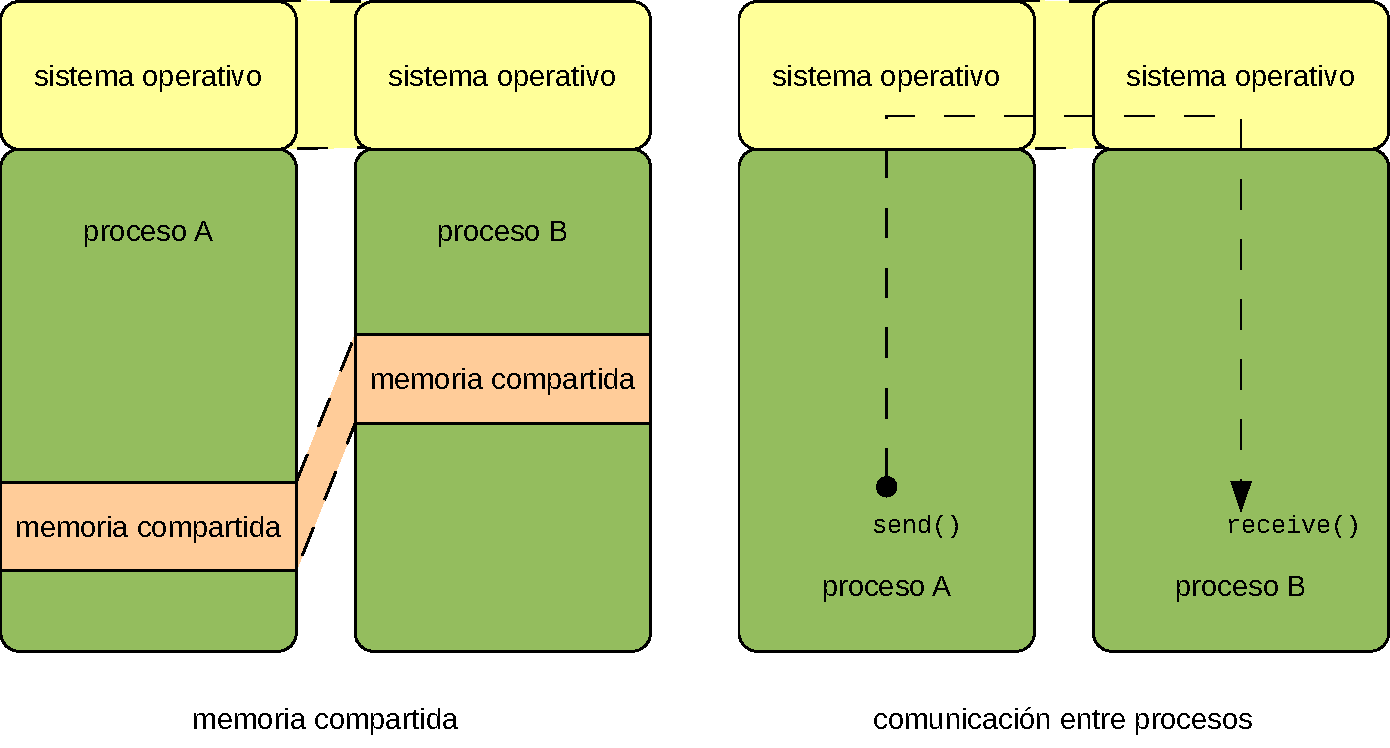
\includegraphics[width=0.8\textwidth]{media/C09_procesos/modelos_comunicación.pdf}
\caption{Modelos de comunicación.}\label{fig-modelos-de-comunicacion}
\end{figure}

\include{capitulos/C10_ipc}
\section{}

\textbf{Tiempo de lectura:} \{s11-reading-time\}

La \textbf{memoria compartida}{} es una estrategia para comunicar
procesos donde uno de ellos gana acceso a regiones de la memoria del
otro; algo que por lo general el sistema operativo siempre intenta
evitar. Por eso, para que pueda haber memoria compartida es necesario
que los dos procesos estén de acuerdo en eliminar dicha restricción.

Dos procesos que comparten una región de la memoria pueden intercambiar
información simplemente leyendo y escribiendo datos en la misma. Sin
embargo debemos tener en cuenta que:

\begin{itemize}
\item
  La estructura de los datos y su localización dentro de la región
  compartida la determinan los procesos en comunicación y no el sistema
  operativo, a diferencia de lo que ocurre en los sistemas de paso de
  mensajes.
\item
  Los procesos son responsables de sincronizarse para no escribir y leer
  en el mismo sitio de la memoria al mismo tiempo, pues esto puede
  generar inconsistencias (véase el \hyperref[sincronizaciuxf3n]{???}) .
\end{itemize}

Las principales ventajas de la memoria compartida frente a otros
mecanismos de comunicación son:

\begin{itemize}
\item
  \textbf{Eficiencia}. Puesto que la comunicación tiene lugar a la
  velocidad de la memoria principal, se trata de un mecanismo
  tremendamente rápido.
\item
  \textbf{Conveniencia}. Puesto que el mecanismo de comunicación solo
  requiere leer y escribir de la memoria, se trata de un sistema muy
  sencillo y fácil de utilizar.
\end{itemize}

Como ocurre con las tuberías (véase el \hyperref[_tuberuxedas]{???}) la
memoria compartida puede ser anónima o con nombre.

\section{Memoria compartida
anónima}\label{_memoria_compartida_anuxf3nima}

La \textbf{memoria compartida anónima}{} solo existe para el proceso que
la crea y para sus procesos hijos, que heredan el acceso. Es por tanto,
una forma eficiente de comunicar procesos padres e hijos.

En los sistemas POSIX, las funciones y operadores de reserva de memoria
como \{clang\_malloc\} y \{cpp\_new\}, utilizan internamente la llamada
al sistema \{linux\_mmap\}. Esta función se puede llamar de la siguiente
manera para reservar \texttt{length} bytes de memoria.

\begin{Shaded}
\begin{Highlighting}[]
\DataTypeTok{void}\OperatorTok{*}\NormalTok{ p }\OperatorTok{=}\NormalTok{ mmap}\OperatorTok{(} 
\NormalTok{    NULL}\OperatorTok{,}
\NormalTok{    length}\OperatorTok{,}     
\NormalTok{    PROT\_READ }\OperatorTok{|}\NormalTok{ PROT\_WRITE}\OperatorTok{,}      
\NormalTok{    MAP\_ANONYMOUS }\OperatorTok{|}\NormalTok{ MAP\_PRIVATE}\OperatorTok{,} 
    \OperatorTok{{-}}\DecValTok{1}\OperatorTok{,}
    \DecValTok{0}
\OperatorTok{);}
\end{Highlighting}
\end{Shaded}

\begin{itemize}
\item
  Si todo va bien, \{linux\_mmap\} devuelve un puntero al primer byte de
  la memoria reservada.
\item
  Cantidad de memoria a reservar en bytes.
\item
  Permisos de acceso para la memoria reservada. En este caso, se
  solicita permitir la lectura y la escritura de la memoria.
\item
  \texttt{MAP\_ANONYMOUS} indica que la memoria no está respaldada por
  ningún archivo, por lo que su contenido inicial será cero. Mientras
  que \texttt{MAP\_PRIVATE} establece que la región de memoria es
  privada.
\end{itemize}

Lo interesante es que si se cambia \texttt{MAP\_PRIVATE} por
\texttt{MAP\_SHARED} la región de memoria reservada es memoria
compartida:

\begin{Shaded}
\begin{Highlighting}[]
\DataTypeTok{void}\OperatorTok{*}\NormalTok{ p }\OperatorTok{=}\NormalTok{ mmap}\OperatorTok{(}
\NormalTok{    NULL}\OperatorTok{,}
\NormalTok{    length}\OperatorTok{,}
\NormalTok{    PROT\_READ }\OperatorTok{|}\NormalTok{ PROT\_WRITE}\OperatorTok{,}
\NormalTok{    MAP\_ANONYMOUS }\OperatorTok{|}\NormalTok{ MAP\_SHARED}\OperatorTok{,} 
    \OperatorTok{{-}}\DecValTok{1}\OperatorTok{,}
    \DecValTok{0}
\OperatorTok{);}
\end{Highlighting}
\end{Shaded}

\begin{itemize}
\item
  Memoria anónima y compartida.
\end{itemize}

Es decir, que al crear un hijo con \{linux\_fork\} este tendrá una copia
de toda la memoria del proceso padre, excepto esta región en particular,
que será la misma que la del padre. Por lo tanto, escribiendo y leyendo
en esa región, ambos procesos pueden comunicarse.

En \{anom\_shared\_memory\_cpp\} se puede ver un ejemplo muy simple,
similar a \{fork\_pipe\_cpp\} pero utilizando memoria compartida para
comunicar ambos procesos. Como se puede apreciar, la versión que usa
memoria compartida es bastante más sencilla que la que utiliza tuberías.

En Microsoft Windows se puede hacer algo similar con
\{win32\_createfilemapping\}:

\begin{Shaded}
\begin{Highlighting}[]
\NormalTok{HANDLE hMapFile }\OperatorTok{=}\NormalTok{ CreateFileMapping}\OperatorTok{(} 
\NormalTok{    INVALID\_HANDLE\_VALUE}\OperatorTok{,}
\NormalTok{    NULL}\OperatorTok{,}
\NormalTok{    PAGE\_READWRITE}\OperatorTok{,} 
    \DecValTok{0}\OperatorTok{,}
\NormalTok{    length}\OperatorTok{,}         
\NormalTok{    NULL}
\OperatorTok{);}
\end{Highlighting}
\end{Shaded}

\begin{itemize}
\item
  Permisos de acceso para la memoria reservada.
\item
  Cantidad de memoria a reservar en bytes.
\item
  A diferencia de \{linux\_mmap\}, \{win32\_createfilemapping\} crea un
  objeto de memoria compartida, pero no hace visible esa memoria para
  nuestro proceso. Para eso hay que llamar a \{win32\_mapviewoffile\}
  pasándole el manejador \texttt{hMapFile} devuelto por
  \{win32\_createfilemapping\}.
\end{itemize}

\section{Memoria compartida con
nombre}\label{_memoria_compartida_con_nombre}

La \textbf{memoria compartida con nombre}{} es pública para el resto del
sistema, por lo que teóricamente cualquier proceso con permisos puede
acceder a ella para comunicarse con otros procesos.

Como ocurre en las tuberías con nombre, los \textbf{objetos de memoria
compartida con nombre} hay que crearlos antes de comenzar a utilizarlos.
Para eso los sistemas POSIX ofrecen la función \{linux\_shm\_open\}.

\begin{Shaded}
\begin{Highlighting}[]
\DataTypeTok{int}\NormalTok{ shmfd }\OperatorTok{=}\NormalTok{ shm\_open}\OperatorTok{(}   
    \StringTok{"/foo{-}shm"}\OperatorTok{,}         
\NormalTok{    O\_RDWR }\OperatorTok{|}\NormalTok{ O\_CREAT}\OperatorTok{,}   
    \BaseNTok{0666}                
\OperatorTok{);}
\end{Highlighting}
\end{Shaded}

\begin{itemize}
\item
  Nombre que identifica al objeto de memoria compartida. Como ocurre con
  los archivos, varios procesos pueden acceder al mismo objeto indicando
  el mismo nombre.
\item
  Valores que indican diferentes opciones a la hora de abrir el objeto.
  Por ejemplo, usando \texttt{O\_RDWR} indicamos que se abra para
  lectura y escritura. Mientras que con \texttt{O\_CREAT} se indica que
  el objeto debe crearse si no existía previamente.
\item
  Indica los permisos del objeto de memoria compartida al crearlo nuevo,
  de forma similar a los permisos que se aplican a los archivos en el
  sistema de archivos.
\end{itemize}

El valor devuelto por \{linux\_shm\_open\} es el descriptor del objeto
de memoria compartida, que utilizaremos posteriormente con
\{linux\_mmap\} al reservar una región de la memoria de nuestro proceso
donde ese objeto de memoria compartida será visible:

\begin{Shaded}
\begin{Highlighting}[]
\DataTypeTok{void}\OperatorTok{*}\NormalTok{ p }\OperatorTok{=}\NormalTok{ mmap}\OperatorTok{(}
\NormalTok{    NULL}\OperatorTok{,}
\NormalTok{    length}\OperatorTok{,}                 
\NormalTok{    PROT\_READ }\OperatorTok{|}\NormalTok{ PROT\_WRITE}\OperatorTok{,}
\NormalTok{    MAP\_SHARED}\OperatorTok{,}             
\NormalTok{    shmfd}\OperatorTok{,}                  
    \DecValTok{0}                       
\OperatorTok{);}
\end{Highlighting}
\end{Shaded}

\begin{itemize}
\item
  Al pasar el descriptor del objeto de memoria compartida, ya no se
  puede indicar \texttt{MAP\_ANONYMOUS}.
\item
  Se puede hacer visible para el proceso todo el objeto de memoria
  compartida o solo una parte. Para esto último se indica el tamaño de
  la región y el desplazamiento dentro del objeto, que es el último
  argumento de \{linux\_mmap\}.
\end{itemize}

Un objeto de memoria compartida recién creado tiene tamaño 0. Para
redimensionarlo se utiliza \{linux\_ftruncate\}, que lo que necesita es
el descriptor del objeto y el nuevo tamaño.

En \{shared\_memory\_cpp\} se puede ver el ejemplo de un programa que
muestra periódicamente la hora del sistema. En este caso controlado por
\{shared\_memory\_control\_cpp\} mediante memoria compartida.

En Microsoft Windows también se utiliza \{win32\_createfilemapping\}
para crear el objeto de memoria compartida con nombre. Simplemente hay
que indicar el nombre en el último argumento de la función.

\begin{Shaded}
\begin{Highlighting}[]
\NormalTok{HANDLE hMapFile }\OperatorTok{=}\NormalTok{ CreateFileMapping}\OperatorTok{(}
\NormalTok{    INVALID\_HANDLE\_VALUE}\OperatorTok{,}
\NormalTok{    NULL}\OperatorTok{,}
\NormalTok{    PAGE\_READWRITE}\OperatorTok{,}
    \DecValTok{0}\OperatorTok{,}
\NormalTok{    length}\OperatorTok{,}
    \StringTok{"Global}\SpecialCharTok{\textbackslash{}\textbackslash{}}\StringTok{FooMemoriaCompartida"} 
\OperatorTok{);}
\end{Highlighting}
\end{Shaded}

\begin{itemize}
\item
  Nombre del nuevo objeto de memoria compartida.
\end{itemize}

\section{}

\textbf{Tiempo de lectura:} \{s12-reading-time\}

En el modelo de proceso que hemos descrito hasta el momento, cada
proceso tiene una única secuencia de instrucciones que se ejecuta en la
CPU. Si los procesos solo pueden tener una única secuencia de
instrucciones, solo pueden realizar una tarea a la vez. Por ejemplo, en
un procesador de textos en un sistema operativo con este modelo de
procesos, el usuario nunca podría escribir al mismo tiempo que se
comprueba la ortografía. En ese caso, si queremos hacer varias tareas al
mismo tiempo, estamos obligados a crear varios procesos y seleccionar un
mecanismo de comunicación para que estos colaboren.

Por eso muchos sistemas operativos modernos han extendido el concepto de
proceso para permitir que cada uno tenga múltiples secuencias de
instrucciones para ejecutarse en la CPU. A cada una de estas secuencias
de instrucciones se las conoce como \textbf{{}hilo} de ejecución. Los
procesos con varios hilos pueden realizar varias tareas a la vez.

\section{Introducción}\label{_introducciuxf3n}

Desde que introducimos el concepto de \textbf{{}proceso} hemos
considerado que es la unidad básica de uso de la CPU. Es decir, que la
CPU se asignaba a los procesos, que la usaban para ejecutar sus
instrucciones. Sin embargo, en los \textbf{sistemas operativos
multihilo}{} es el \textbf{hilo} la unidad básica de uso de la CPU.

\begin{figure}
\centering
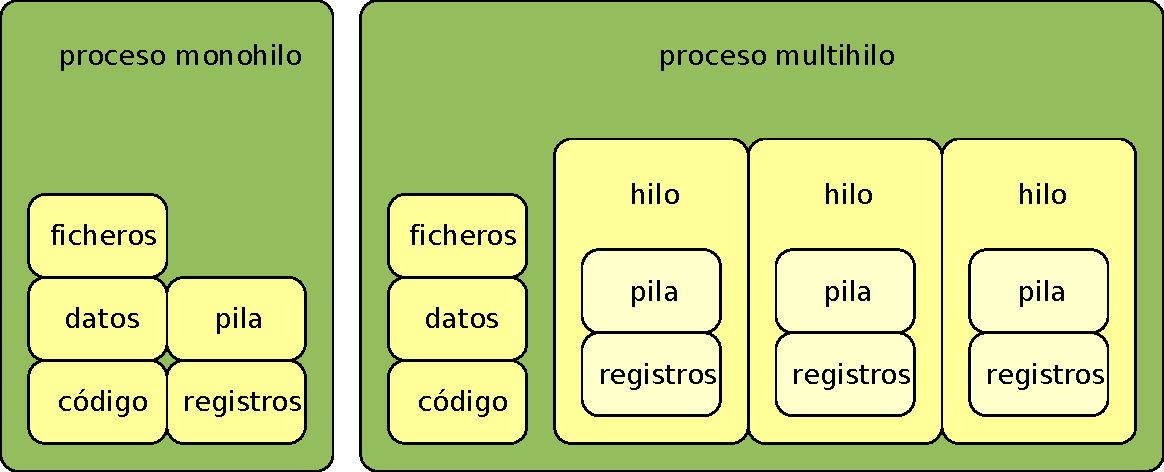
\includegraphics[width=0.8\textwidth]{media/C12_hilos/procesos_multihilo.pdf}
\caption{Esquema comparativo entre procesos monohilo y proceso
multihilo.}\label{fig-multihilo}
\end{figure}

Cada hilo tiene una serie de recursos propios dentro del proceso (véase
la \hyperref[fig-multihilo]{Esquema comparativo entre procesos monohilo
y proceso multihilo.}):

\begin{itemize}
\item
  \textbf{El identificador del hilo} es único para cada hilo y sirve
  para identificarlos, de la misma manera que lo hace el identificador
  de proceso con cada proceso.
\item
  \textbf{El contador de programa} es el registro de la CPU que indica
  la dirección de la próxima instrucción del hilo que debe ser ejecutada
  por la CPU.
\item
  \textbf{Los registros de la CPU}, cuyos valores son diferentes en cada
  hilo, puesto que, aunque todos los hilos ejecutan el mismo programa,
  pueden ejecutar diferentes partes del mismo.
\item
  \textbf{La pila} contiene datos temporales como argumentos y
  direcciones de retorno de las funciones y variables locales. Al igual
  que ocurre con los registros de la CPU, cada hilo necesita su pila
  porque recorre el programa de manera diferente.
\end{itemize}

Sin embargo hay otros recursos que se asignan al proceso, por lo que se
comparten entre todos los hilos del mismo (véase la
\hyperref[fig-multihilo]{Esquema comparativo entre procesos monohilo y
proceso multihilo.}):

\begin{itemize}
\item
  \textbf{El código del programa}. El programa es el mismo para todos
  los hilos.
\item
  \textbf{Los segmentos BSS y de datos y el montón}. Las secciones de
  datos diferentes de la pila son accesibles a todos los hilos. Eso
  quiere decir, por ejemplo, que cualquier hilo puede acceder y
  modificar una variable global o una asignada dinámicamente mediante
  \{clang\_malloc\} o \{cpp\_new\}.
\item
  \textbf{Otros recursos del proceso} como archivos, \emph{sockets},
  tuberías y dispositivos abiertos, regiones de memoria compartida,
  señales, directorio actual de trabajo, entre muchos otros recursos.
\end{itemize}

Esto significa que cada instante, en cada CPU del sistema se puede estar
ejecutando un hilo, del mismo o de distintos procesos en el sistema;
pero la memoria, los archivos y otros recursos pertenecen al proceso del
que cada uno forma parte. Si un hilo reserva memoria o abre un archivo o
un dispositivo y no lo libera antes de terminar, el recurso permanecerá
reservado, no siendo liberado hasta que lo haga otro hilo o el proceso
completo termine. Si un hilo ejecuta una instrucción privilegiada o
intenta acceder a una zona de memoria para la que no tiene permiso, la
condición de error se propaga a todo el proceso. Por tanto, por lo
general, el sistema operativo detendrá el proceso completo del que
formaba parte.

Si se quiere ejecutar varias tareas al mismo tiempo de forma que la
fiabilidad sea máxima, haciendo que los errores en unas no puedan
afectar a las otras, tendremos que olvidarnos de los hilos. Debemos
utilizar diferentes procesos para cada tarea. Así cada tarea tiene sus
propios recursos y su propio espacio de direcciones virtual, lo que
aísla a unas tareas de las otras.

\begin{figure}
\centering
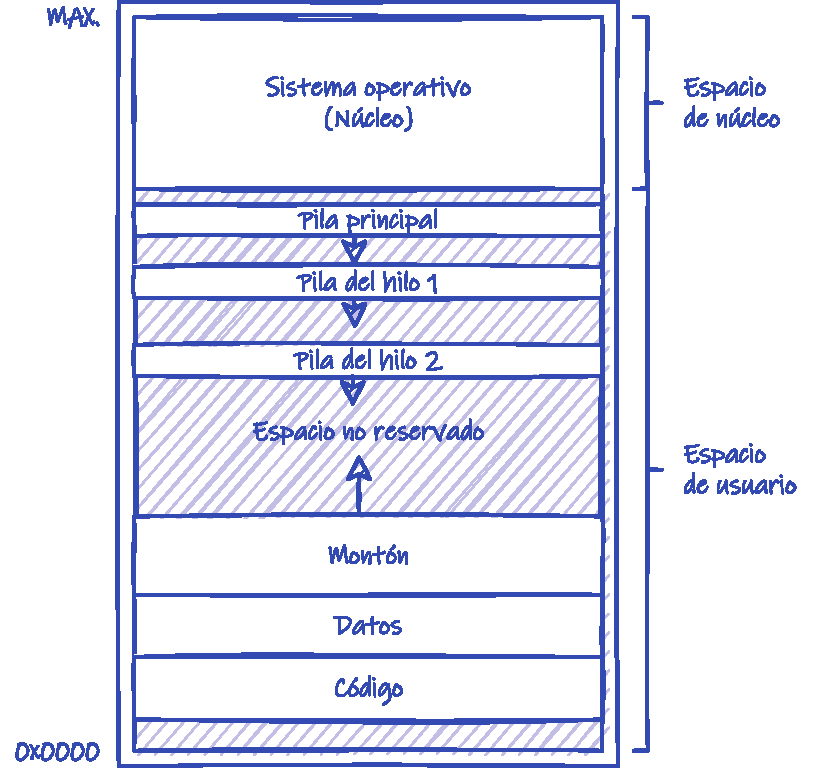
\includegraphics[width=0.8\textwidth]{media/C12_hilos/proceso_multihilo_en_memoria.pdf}
\caption{Anatomía de un proceso multihilo en
memoria.}\label{fig-proceso-multihilo-en-memoria}
\end{figure}

En la \hyperref[fig-proceso-multihilo-en-memoria]{Anatomía de un proceso
multihilo en memoria.} se puede observar como cambia la disposición de
los elementos de un proceso en la memoria cuando es multihilo, respecto
a lo que vimos en el \hyperref[_el_proceso]{???}.

\section{Beneficios}\label{_beneficios}

Son muchos los beneficios que aporta la programación multihilo,
derivados de que ofrece una forma sencilla de que un único proceso pueda
realizar varias tareas al mismo tiempo.

\subsection{Tiempo de respuesta}\label{_tiempo_de_respuesta}

Una aplicación multihilo interactiva puede continuar ejecutando tareas
aunque uno o varios hilos de la misma estén bloqueados o realizando
operaciones muy lentamente, mejorando así el tiempo de respuesta al
usuario.

Por ejemplo, un navegador web multihilo puede gestionar la interacción
del usuario a través de un hilo, mientras el contenido solicitado se
descarga en otro. Para hacer lo mismo en un navegador monohilo habría
que utilizar comunicaciones asíncronas, de lo contrario, mientras el
proceso está en estado \textbf{esperando}, a la espera de que lleguen
los datos a través de la red, no puede atender las acciones del usuario.

El uso de comunicaciones asíncronas para obtener el mismo beneficio
tiene menor coste que usar hilos, pero son más difíciles de programar.

\subsection{Compartición de
recursos}\label{_comparticiuxf3n_de_recursos}

Los hilos no son la única forma de conseguir que un programa realice
varias tareas al mismo tiempo. Una alternativa es que un mismo programa
cree varios procesos hijo, que se comuniquen y coordinen entre sí, para
hacer distintas tareas.

Sin embargo, aunque la programación multiproceso ofrece beneficios
similares a la multihilo, en esta última la comunicación es mucho más
sencilla porque los hilos comparten automáticamente los recursos del
proceso al que pertenecen. De hecho, los hilos no solo comparten la
memoria, sino también otros muchos recursos del proceso, como los
archivos y los dispositivos abiertos. Por lo que los hilos son una forma
más conveniente de ejecutar múltiples tareas al mismo tiempo, que la
programación multiproceso.

Como contrapartida, la programación multiproceso es más fiable, ya que
los errores en un proceso no afectan al resto. Es decir, si un proceso
hijo termina de forma inesperada, el proceso padre puede continuar
ejecutándose sin problemas e incluso crear un nuevo proceso hijo para
sustituir al que ha terminado.

\subsection{Economía}\label{_economuxeda}

Reservar memoria y otros recursos para la creación de un proceso es muy
costoso. Por eso los sistemas operativos modernos han desarrollado
diversas técnicas para que sea lo más eficaz posible.

Aun así, puesto que los hilos comparten los recursos de los procesos a
los que pertenecen, son mucho más económicos de crear. También es más
económico el cambio de contexto entre ellos, ya que hay que guardar y
recuperar menos información a conmutar la ejecución en la CPU entre dos
hilos de un mismo proceso, que entre dos procesos diferentes.

Por ejemplo, en Microsoft Windows crear un proceso puede ser 300 veces
más costoso que un hilo. Mientras que en sistemas Linux es 3 veces más
lento, por la eficiencia de \{linux\_fork\}.

\subsection{Aprovechamiento de las arquitecturas
multiprocesador}\label{_aprovechamiento_de_las_arquitecturas_multiprocesador}

En los sistemas multiprocesador diferentes hilos pueden ejecutarse en
paralelo en distintos procesadores. Por el contrario, un proceso
monohilo solo se puede ejecutar en una CPU a la vez, independientemente
de cuantas CPU estén disponibles para ejecutarlo.

Nuevamente, en los sistemas monohilo se pueden utilizar varios procesos
para aprovechar las arquitecturas multiprocesador. Sin embargo, como
hemos comentado anteriormente, los hilos son más fáciles de programar y
más económicos de crear y gestionar que los procesos.

\subsection{Comparación con soluciones
alternativas}\label{_comparaciuxf3n_con_soluciones_alternativas}

A modo de resumen, los hilos son una forma sencilla de que un único
proceso pueda realizar varias tareas al mismo tiempo, pero no son la
única:

\begin{itemize}
\item
  El uso de \textbf{comunicaciones asíncronas} permite realizar varias
  tareas de E/S al mismo tiempo, sin necesidad de hilos. Suele ser una
  opción más económica que usar hilos, pero también es más difícil de
  programar.
\item
  El uso de \textbf{múltiples procesos} permite realizar varias tareas
  al mismo tiempo, tanto de E/S como de cálculo, y de forma más fiable
  que los hilos. Sin embargo, los procesos suelen ser más caros de crear
  y gestionar que los hilos y no comparten los recursos de forma
  automática, por lo que la comunicación entre ellos es algo más
  complicada.
\end{itemize}

\section{Soporte multihilo}\label{_soporte_multihilo}

Las \textbf{librerías de hilos}{} proporcionan al programador la
interfaz de programación para crear y gestionar los hilos de un proceso.
Por lo general, mediante lenguaje C se puede acceder directamente a la
\textbf{librería de hilos} del sistema. Otros lenguajes proporcionan un
\textbf{librería de hilos} dentro de su \textbf{librería estandar}, que
a su vez se apoya en la \textbf{librería de hilos} del sistema
operativo.

El soporte de hilos en un sistema operativo se puede proporcionar a
\textbf{nivel de usuario} o a \textbf{nivel de núcleo}.

\subsection{Hilos a nivel de usuario}\label{_hilos_a_nivel_de_usuario}

{} El soporte de \textbf{hilos a nivel de usuario} se implementan
mediante un \textbf{librería de hilos} en el espacio de usuario, junto
al código del programa y los datos del proceso, sin requerir ningún
soporte especial por parte del núcleo del sistema operativo. Por tanto,
como se puede observar en el lado derecho de la
\hyperref[fig-comparaciuxf3n-soporte-de-hilos]{Comparación de hilos a
nivel de usuario y a nivel de núcleo.}, estos hilos existen desde el
punto de vista del proceso y del programa que ejecuta, pero no para el
sistema operativo. El planificador de la CPU asigna tiempo de CPU a los
procesos, mientras que la \textbf{librería de hilos} de cada proceso
reparte el tiempo de ejecución del proceso entre los diferentes hilos de
este.

\begin{figure}
\centering
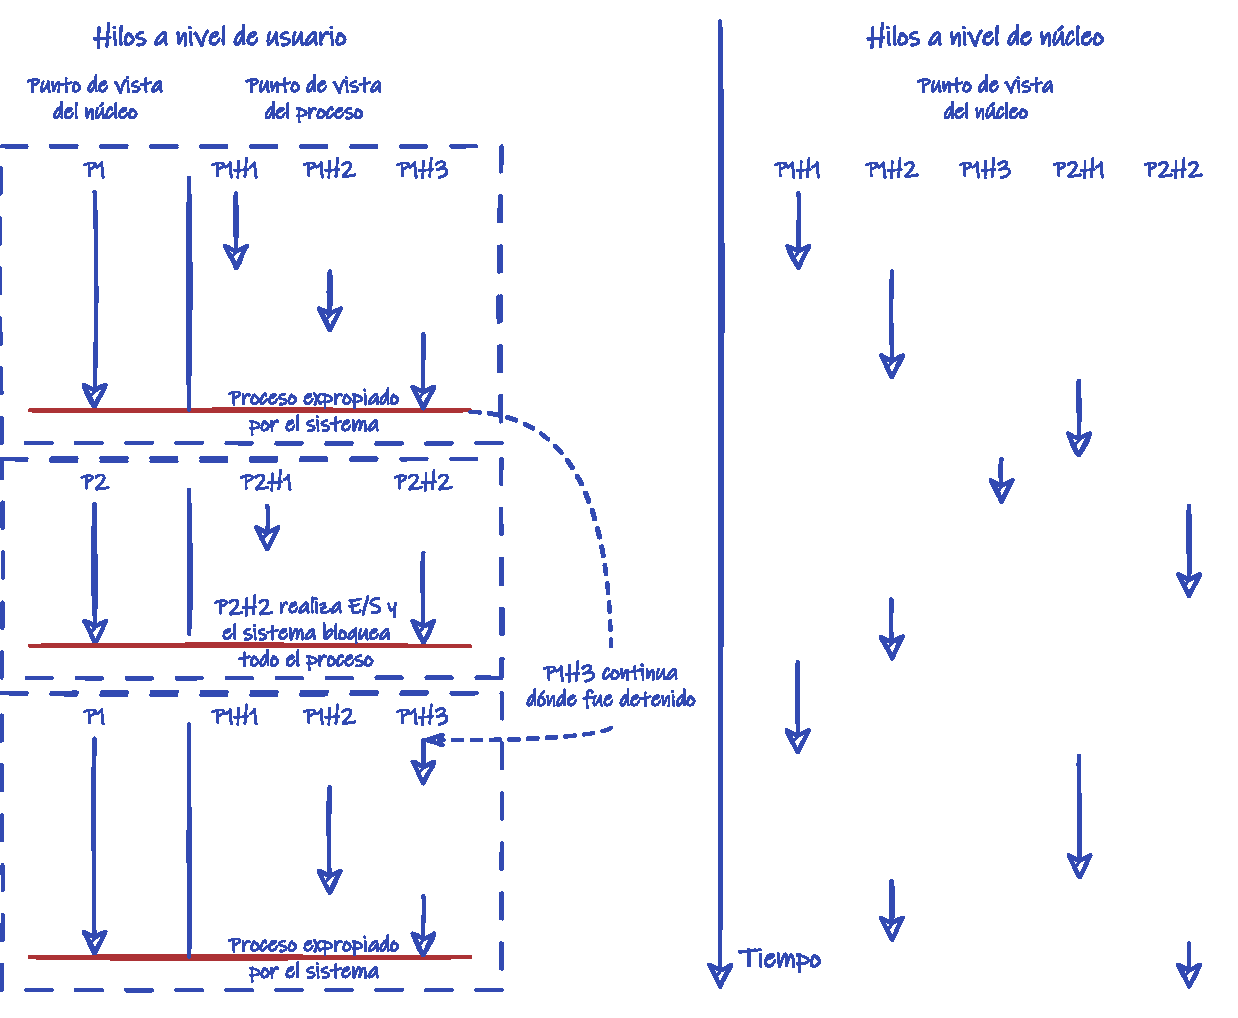
\includegraphics[width=0.8\textwidth]{media/C12_hilos/comparación_soporte_de_hilos.pdf}
\caption{Comparación de hilos a nivel de usuario y a nivel de
núcleo.}\label{fig-comparaciuxf3n-soporte-de-hilos}
\end{figure}

Como el código y los datos de la librería residen en el espacio de
usuario, invocar una función de la misma se reduce a una simple llamada
a una función, evitando el coste de hacer llamadas al sistema.

\subsection{Hilos a nivel de núcleo}\label{_hilos_a_nivel_de_nuxfacleo}

{} Se habla de \textbf{hilos a nivel de núcleo}, cuando el núcleo del
sistema es el encargado de ofrecer el soporte multihilo. El código y los
datos de la \textbf{librería de hilos}, mediante la cual los
programadores pueden solicitar la creación y gestión de los hilos,
reside en el espacio del núcleo. Por tanto, para invocar una función de
la \textbf{librería de hilos} es necesario hacer una llamada al sistema.
Obviamente, la librería del sistema ofrece las funciones necesarias para
realizar estas llamadas al sistema de forma sencilla.

La implementación del soporte de hilos en el núcleo implica cambios
respecto a lo que hemos visto hasta el momento de la gestión de
procesos, puesto que, en estos sistemas, es el hilo la unidad básica de
uso de la CPU, como se ilustra en la
\hyperref[fig-comparaciuxf3n-soporte-de-hilos]{Comparación de hilos a
nivel de usuario y a nivel de núcleo.}. Es decir, son los hilos los que
se mueven por los estados del
\hyperref[fig-diagrama-estado-proceso]{???} y las colas de la
\hyperref[fig-colas-de-planificaciuxf3n-procesos]{???}, en lugar de los
procesos. En estos sistemas, el planificador de la CPU selecciona un
hilo para ejecutarse en la CPU de entre todos los que están en el estado
\textbf{preparado} en el sistema y el \textbf{cambio de contexto} asigna
la CPU a un hilo distinto al que la tiene asignada en el momento actual,
que puede ser del mismo o de diferente proceso.

Aparte del \textbf{PCB} que vimos en el
\hyperref[_bloque_de_control_de_proceso]{???}, ahora el sistema
operativo también gestiona una estructura llamada \textbf{bloque de
control del hilo}{} o {}TCB (\emph{Thread Control Block}) para cada hilo
en el sistema, donde se guarda información sobre su estado de actividad
actual. Por tanto, es en \textbf{TCB} ---y no en el \textbf{PCB}---
donde se guarda la información privada del hilo necesaria para la
gestión de los estados y para el cambio de contexto, como: los valores
de los registros de la CPU y el contador de programa, el estado o la
información de planificación de la CPU; además de un puntero al
\textbf{PCB} al que pertenece el hilo con el resto de la información
privada del proceso.

\subsection{Implementaciones}\label{_implementaciones}

En la actualidad, en los diferentes sistemas operativos se pueden
encontrar librerías de ambos tipos.

Por ejemplo, la librería de hilos de Windows API se implementa en el
núcleo\hyperref[Win32-UsingProcessesAndThreads]{???} mientras que la
librería de hilos \{pthreads\} ---frecuentemente utilizada en los
sistemas POSIX--- puede ser de ambos tipos, dependiendo solamente del
sistema donde se implemente. En Linux y en la mayor parte de los UNIX
modernos, POSIX Threads se implementa en el núcleo del sistema.

\section{Modelos multihilo}\label{_modelos_multihilo}

En base a lo anterior, sabemos que hay sistemas que implementan
\textbf{hilos a nivel de núcleo} mientras otros los hacen a
\textbf{nivel de usuario}. Sin embargo, también existen sistemas donde
se combinan ambos.

Para comparar las diferentes opciones que tienen los diseñadores de un
sistema en cuanto al soporte de hilos, se definen los \textbf{modelos
multihilo} en base a la relación entre \textbf{hilos de usuario} e
\textbf{hilos de núcleo}. Aquí entendemos por \textbf{hilos de núcleo} a
estas secuencias de instrucciones tal y como las ve el programa en el
espacio de usuario. Mientras que el concepto de \textbf{hilos de núcleo}
corresponde con como las ve el núcleo del sistema.

\subsection{Muchos a uno (N:1)}\label{_muchos_a_uno_n1}

{} {} En el modelo \textbf{muchos a uno} muchos \textbf{hilos de
usuario} son mapeados en \textbf{un único hilo de núcleo}. El
planificador de la CPU en el núcleo reparte el tiempo de CPU entre los
diferentes \textbf{hilos de núcleo} en el sistema, mientras que la
\textbf{librería de hilos} en cada proceso reparte el tiempo de
ejecución del \textbf{hilo de núcleo} del proceso entre múltiples
\textbf{hilos de usuario} (véase la
\hyperref[fig-modelo-muchos-a-uno]{Modelo muchos a uno (N:1).}).

\begin{figure}
\centering
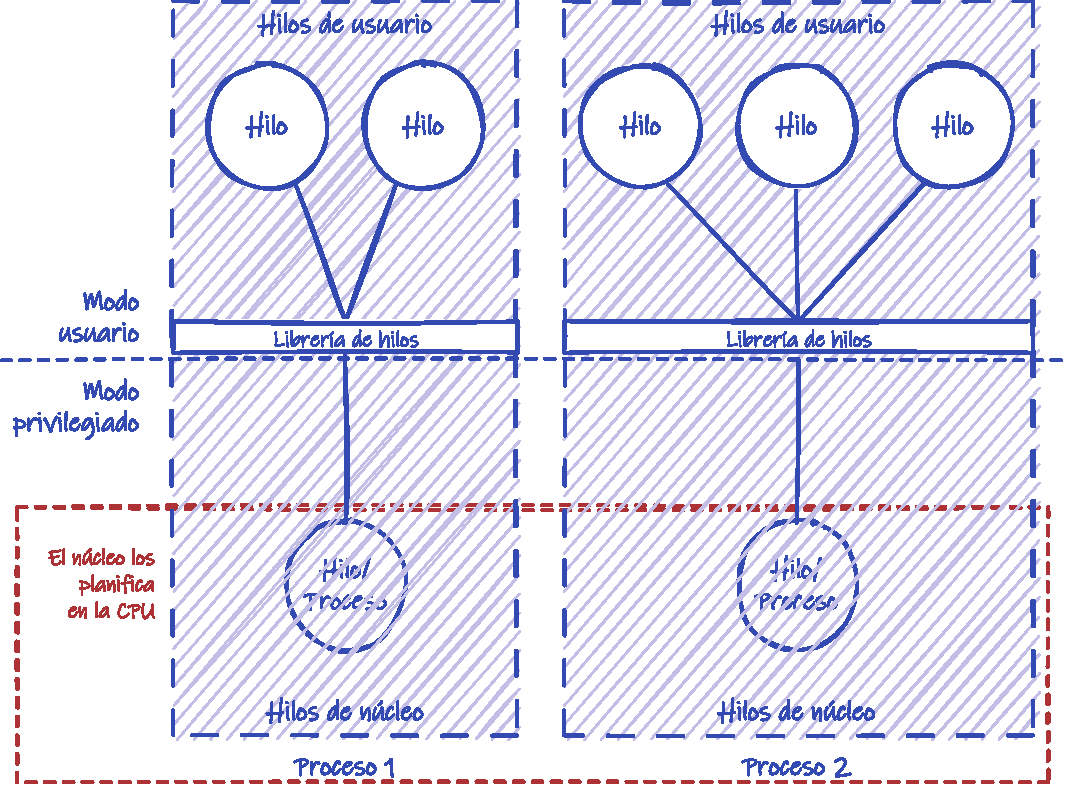
\includegraphics[width=0.8\textwidth]{media/C12_hilos/modelo_muchos_a_uno.pdf}
\caption{Modelo muchos a uno (N:1).}\label{fig-modelo-muchos-a-uno}
\end{figure}

Los sistemas modernos son multihilo, por lo que al crearse un proceso
siempre se crea con un \textbf{hilo de núcleo} inicial, que es al que el
núcleo asigna tiempo de CPU. Sin embargo, los sistemas más antiguos no
tienen ningún soporte de hilos en el núcleo, por lo que no hay
\textbf{hilos de núcleo}. En este sentido, quizás sería más correcto
definir el modelo \textbf{muchos a uno} como aquel en el que muchos
\textbf{hilos de usuario} son mapeados en una «única entidad
planificable en la CPU». En los sistemas más antiguos estas entidades
son los procesos, de forma que, bajo este \textbf{modelo multihilo} los
\textbf{hilos de usuario} realmente se reparten el tiempo de ejecución
del proceso al que pertenecen.

El modelo \textbf{muchos a uno} corresponde al caso en el que solo se
implementan \textbf{hilos a nivel de usuario}, que es el caso ilustrado
a la izquierda en la
\hyperref[fig-comparaciuxf3n-soporte-de-hilos]{Comparación de hilos a
nivel de usuario y a nivel de núcleo.}.

\subsubsection{Ventajas e
inconvenientes}\label{_ventajas_e_inconvenientes}

La principal \textbf{ventaja} de este modelo es su bajo coste, por lo
que resulta ideal cuando la cantidad de hilos a crear ---el nivel de
concurrencia--- va a ser muy alta:

\begin{itemize}
\item
  Los \textbf{hilos de usuario} son muy baratos de crear porque la
  gestión de hilos se hace con una librería en el espacio de usuario,
  dentro del proceso. Mientras que los \textbf{hilos de núcleo} pueden
  necesitar más recursos del sistema, como espacio en la tabla de hilos
  del sistema y en otras estructuras de gestión.
\item
  La invocación de las funciones de la \textbf{librería de hilos} se
  hace por medio de simples llamadas a funciones, que son menos costosas
  que las llamadas al sistema necesarias cuando el soporte de hilos se
  implementa en el núcleo.
\item
  Se necesitan menos cambios de contexto. Los cambios de contexto, que
  ocurren cuando se transfiere el control de la CPU, pueden ser
  operaciones costosas. En el modelo \textbf{muchos a uno} pueden
  ocurrir cambios de contexto en el núcleo al intercambiar procesos en
  la CPU, pero el intercambio de hilos se gestiona en el propio proceso,
  lo que suele ser más rápido que hacerlo en el núcleo.
\end{itemize}

Mientras que estos son algunos posibles \textbf{inconvenientes}:

\begin{itemize}
\item
  Los hilos de un mismo proceso no se pueden ejecutar en paralelo en
  sistemas multiprocesador, por lo que este modelo no permite aprovechar
  ese tipo de sistemas. El motivo es que la librería de hilos en espacio
  de usuario no tiene acceso a los procesadores del sistema. Solo conoce
  el proceso en el que se ejecuta y reparte el tiempo de ejecución del
  proceso entre los distintos hilos.

  El núcleo del sistema si ve los diferentes procesadores, pero
  desconoce la existencia de los hilos dentro de los procesos. Solo ve
  procesos que deben ejecutarse en las distintas CPU.
\item
  Un hilo puede bloquear la ejecución del resto de los hilos de su
  proceso, en determinadas circunstancias.

  Si uno de los hilos solicita al sistema operativo una operación que
  deba ser bloqueada a la espera ---por ejemplo,operaciones de E/S sobre
  archivos, comunicaciones o esperar a que otro proceso termine--- todo
  el proceso es puesto como \emph{esperando} por el sistema operativo,
  no pudiendo ejecutarse otros hilos del mismo proceso en la CPU,
  mientras tanto. Para evitar en parte este problema, es frecuente que
  las implementaciones de este modelo ofrezcan versiones especiales de
  estas operaciones, con capacidad para evitar el bloqueo total del
  proceso, en función de si el sistema operativo tiene el soporte
  adecuado para ello.
\end{itemize}

Por tanto, este modelo no es una opción si lo que interesa es aprovechar
el paralelismo en sistemas multiprocesador, para intentar realizar
ciertas operaciones en menos tiempo.

\subsubsection{Operaciones bloqueantes}\label{_operaciones_bloqueantes}

El problema del bloqueo de procesos ocasionado por operaciones de E/S
que pongan al proceso en estado \emph{esperando} puede ser evitado
interceptando las llamadas a funciones de la librería del sistema, para
evitar el uso de llamadas al sistema que se puedan bloquear y
sustituirlas por versiones equivalentes pero asíncronas.

Obviamente, la \textbf{librería de hilos} intercambia el \textbf{hilo de
usuario} en ejecución cuando el que se está ejecutando finaliza. Además,
generalmente, tiene funciones para que el \textbf{hilo de usuario} en
ejecución se duerma ---\texttt{sleep()}--- o para que espere a que otro
hilo termine ---\texttt{wait()} o \texttt{join()}. En ambos casos, el
\textbf{hilo de usuario} queda bloqueado y la \textbf{librería de hilos}
asigna otro hilo al \textbf{hilo de núcleo} para su ejecución.

Por ejemplo, en la
\hyperref[fig-modelo-a-uno-operaciuxf3n-bloqueante]{Diagrama de
secuencia del bloqueo del proceso en el modelo muchos a uno.} se ilustra
como el \emph{Hilo 1} llama a la función \texttt{yield()} de la
\textbf{librería de hilos}, provocando su intercambio con el \emph{Hilo
2}. La función \texttt{yield()} suele estar presente en algunas
\textbf{librerías de hilos}, con el objeto de que los hilos puedan
indicar puntos del programa en los que quieren dejar tiempo de ejecución
para otros hilos, de forma voluntaria.

\begin{figure}
\centering
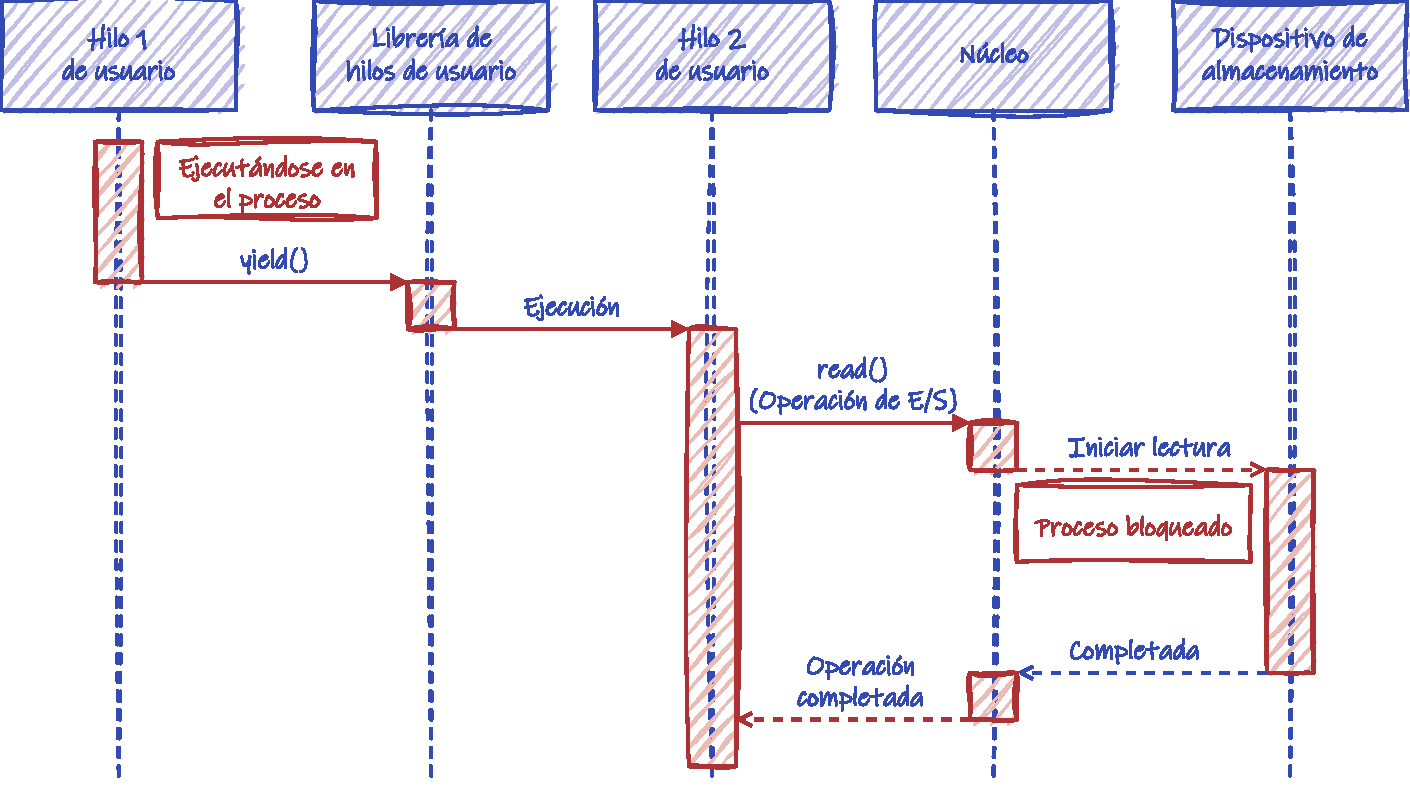
\includegraphics[width=0.8\textwidth]{media/C12_hilos/muchos_a_uno_operación_bloqueante.pdf}
\caption{Diagrama de secuencia del bloqueo del proceso en el modelo
muchos a uno.}\label{fig-modelo-a-uno-operaciuxf3n-bloqueante}
\end{figure}

Sin embargo, en la
\hyperref[fig-modelo-a-uno-operaciuxf3n-bloqueante]{Diagrama de
secuencia del bloqueo del proceso en el modelo muchos a uno.} también
vemos que \emph{Hilo 2} invoca la llamada al sistema \texttt{read()}
para leer un archivo. Desde el punto de vista del núcleo, esa llamada la
realiza el proceso, por lo que es bloqueado, hasta que la operación de
lectura del archivo se completa. Al proceso nunca se le asignará la CPU
mientras esté en estado \emph{esperando}, por lo que ni \emph{Hilo 1} ni
ningún otro \textbf{hilo de usuario} del proceso podrá ejecutarse.

La solución, como hemos comentado, es que la \textbf{librería de hilos}
proporcione sus propias versiones de las llamadas al sistema que pueden
poner al proceso en estado \emph{esperando}. Por ejemplo, en la
\hyperref[fig-modelo-a-uno-operaciuxf3n-bloqueante]{Diagrama de
secuencia del bloqueo del proceso en el modelo muchos a uno.} el
\emph{Hilo 2} no usa la llamada al sistema \texttt{read()} sino una
función \texttt{read()} proporcionada por la \textbf{librería de hilos}.

Para implementar su \texttt{read()}, la \textbf{librería de hilos} usa
una versión asíncrona de la llamada al sistema. Es decir, una versión
donde se le indica al sistema que se quiere hacer una operación de E/S,
pero el proceso no entra en estado de espera mientras ocurre. En su
lugar, el proceso retorna inmediatamente de la llamada al sistema y
sigue ejecutándose en la CPU, lo que permite que la \textbf{librería de
hilos} comience a ejecutar \emph{Hilo 1} en el lugar de \emph{Hilo 2}.
Es decir, desde el punto de vista de \emph{Hilo 2}, la función
\texttt{read()} de la \textbf{librería de hilos} es bloqueante.

\begin{figure}
\centering
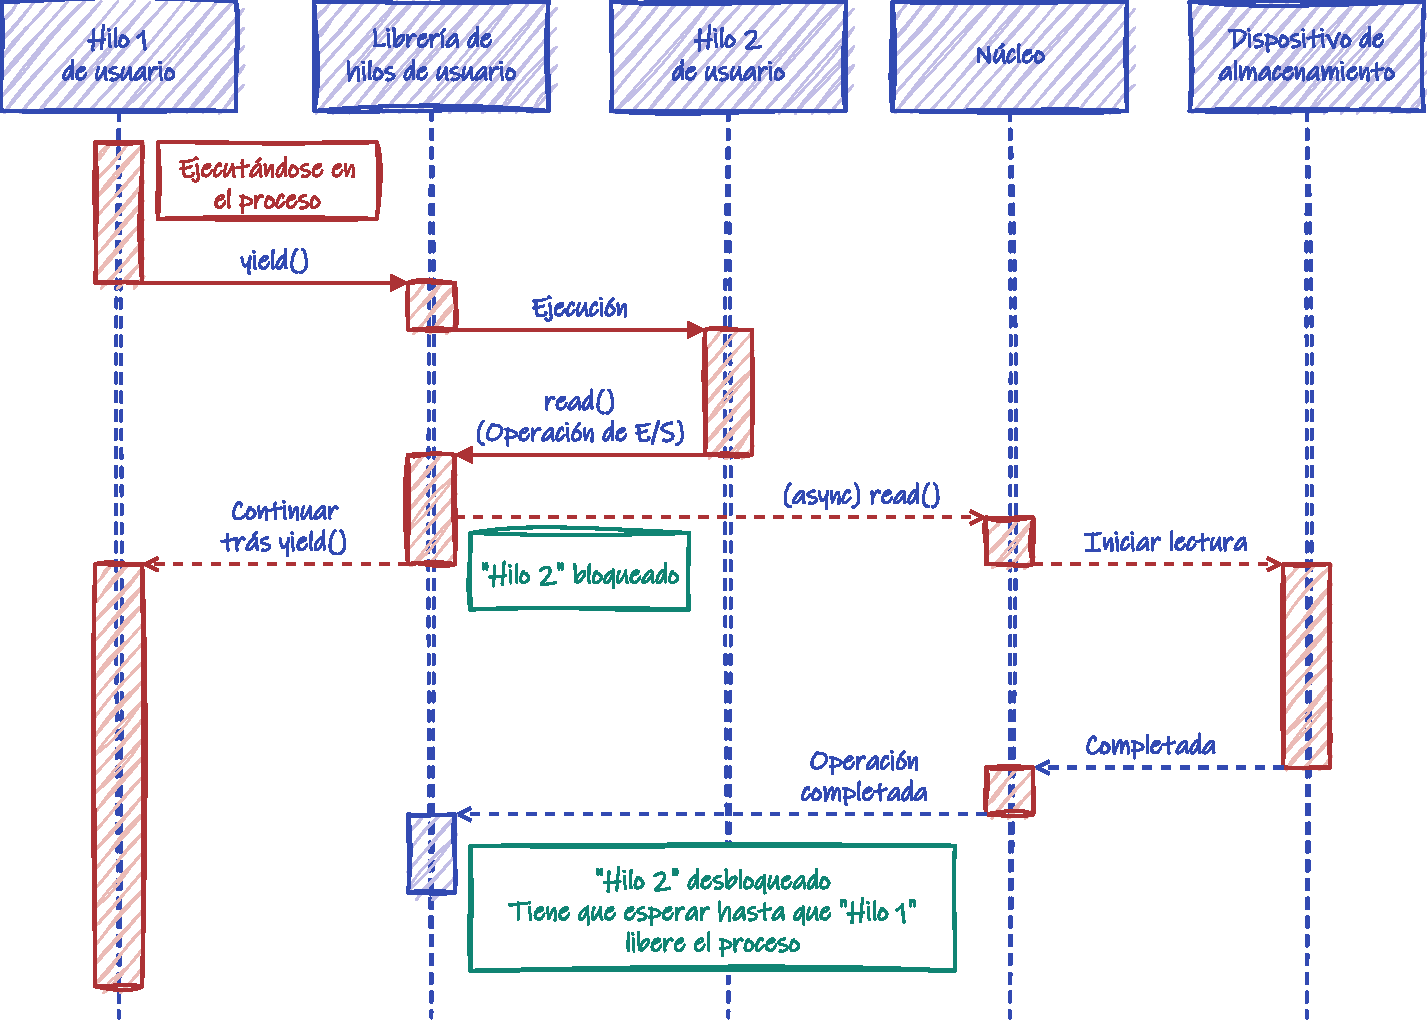
\includegraphics[width=0.8\textwidth]{media/C12_hilos/muchos_a_uno_operación_async.pdf}
\caption{Diagrama de secuencia de la solución al bloqueo del proceso en
el modelo muchos a uno.}\label{fig-modelo-a-uno-operaciuxf3n-async}
\end{figure}

Más adelante, el sistema operativo notificará a la \textbf{librería de
hilos} que la operación ha sido realizada, por lo que los datos ya están
disponibles en la memoria para ser usados. En ese momento, \emph{Hilo 2}
vuelve al estado \emph{preparado} para volver a ser planificado por la
\textbf{librería de hilos} cuando sea posible.

Este procedimiento es complejo y requiere versiones no bloqueantes de
todas las llamadas al sistema, lo que puede que no siempre se cumpla.
Por lo general, cualquier sistema operativo moderno ofrece versiones
asíncronas de todas las operaciones de E/S, pero puede haber otras
llamadas al sistema que puedan poner al proceso en estado
\emph{esperando} y que no tengan versión asíncrona.

\subsubsection{Implementaciones}\label{_implementaciones_2}

A este modelo de hilos también se lo denomina
\href{https://en.wikipedia.org/wiki/Green_threads}{Green Threads}. En
Java 1.1 era el único modelo soportado ---ya que los hilos se
implementaban en la máquina virtual de Java, independientemente del
soporte del sistema operativo--- pero debido a sus limitaciones se
implementó el soporte de hilos nativos del sistema operativo.

Otras implementaciones de este modelo son las
\href{https://docs.microsoft.com/en-us/windows/win32/procthread/fibers}{fibras}
y
\href{https://docs.microsoft.com/en-us/windows/win32/procthread/user-mode-scheduling}{UMS}
de Windows API, \{stackless\_python\} y
\href{http://www.gnu.org/software/pth/}{GNU Portable Threads}.

\subsection{Uno a uno (1:1)}\label{_uno_a_uno_11}

{} {} En el modelo \textbf{muchos a uno} un \textbf{hilo de usuario} se
mapea en \textbf{un único hilo de núcleo}.

Por lo general, este modelo corresponde al caso de los sistemas que solo
soportan \textbf{hilos a nivel de núcleo}. En este caso, la
\textbf{librería de hilos} se implementa en el núcleo, por lo que las
entidades que planifica el núcleo en la CPU son los \textbf{hilos de
núcleo} y los procesos pueden gestionar estos hilos mediante llamadas al
sistema (véase la \hyperref[fig-modelo-uno-a-uno]{Modelo uno a uno
(1:1).}).

\begin{figure}
\centering
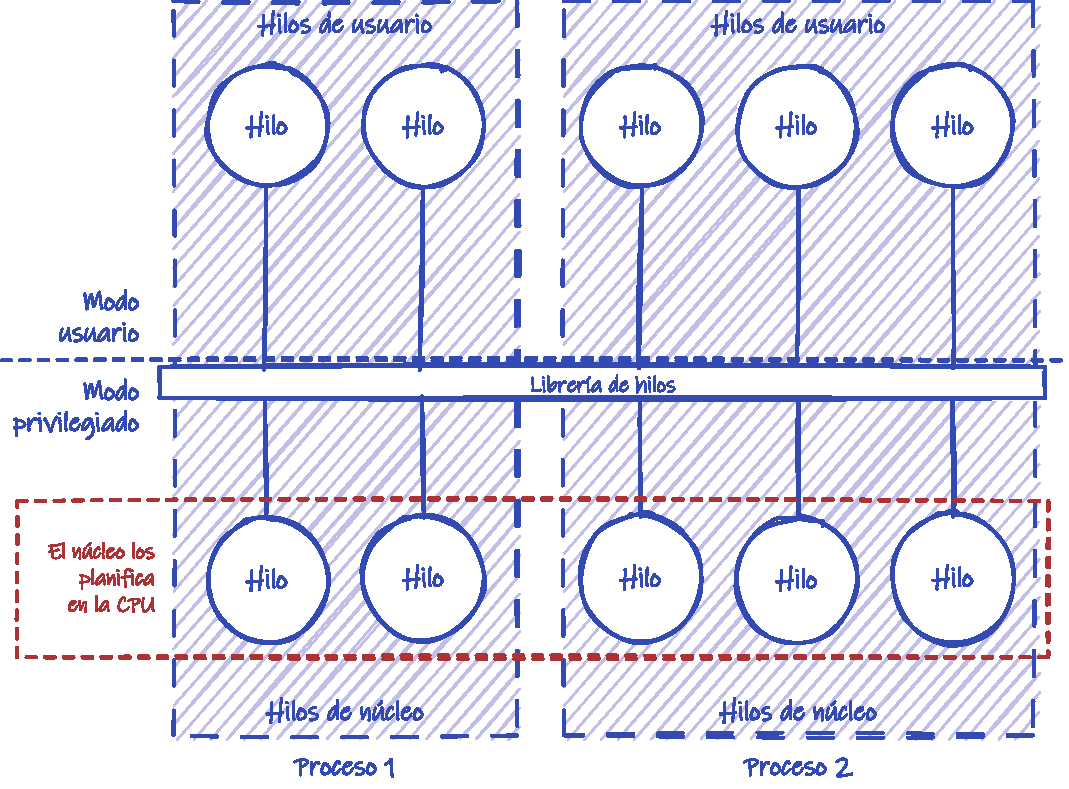
\includegraphics[width=0.8\textwidth]{media/C12_hilos/modelo_uno_a_uno.pdf}
\caption{Modelo uno a uno (1:1).}\label{fig-modelo-uno-a-uno}
\end{figure}

Es importante tener en cuenta que, a efectos prácticos, los
\textbf{hilos de usuario} de la \hyperref[fig-modelo-uno-a-uno]{Modelo
uno a uno (1:1).} no son hilos diferentes a los \textbf{hilos de
núcleo}. Realmente, son los mismos \textbf{hilos de núcleo}, pero vistos
desde la perspectiva del programa en el modo usuario, como se ilustra a
la derecha en la
\hyperref[fig-comparaciuxf3n-soporte-de-hilos]{Comparación de hilos a
nivel de usuario y a nivel de núcleo.}.

\subsubsection{Ventajas e
inconvenientes}\label{_ventajas_e_inconvenientes_2}

Las principales \textbf{ventajas} de este modelo son:

\begin{itemize}
\item
  Permite a otros hilos del mismo proceso ejecutarse aun cuando uno de
  ellos haga una llamada al sistema que debe bloquearse. El núcleo se
  encarga de ponerlo en espera y planificar en la CPU a otro de los
  hilos preparados para ejecutarse de entre todos los existentes en el
  sistema.
\item
  Permite paralelismo en sistemas multiprocesador, ya que diferentes
  hilos pueden ser planificados por el núcleo en distintos procesadores.
\end{itemize}

Mientras que estos son algunos posibles \textbf{inconvenientes}:

\begin{itemize}
\item
  Crear hilos puede tener mayor coste. En este caso, crear un hilo para
  un proceso implica crear y gestionar ciertas estructuras de datos en
  el núcleo. Debido a que la cantidad de memoria disponible para el
  núcleo suele estar limitada, muchos sistemas restringen la cantidad
  máxima de \textbf{hilos de núcleo} soportados.
\item
  La gestión de los hilos se hace con una librería en el espacio de
  núcleo, lo que requiere que el proceso haga llamadas al sistema para
  gestionarlos. Esto suele tener mayor coste que invocar simplemente una
  función, como ocurre en el modelo \textbf{muchos a uno}.
\end{itemize}

\subsubsection{Implementaciones}\label{_implementaciones_3}

El modelo \textbf{uno a uno} se utiliza en la mayor parte de los
sistemas operativos multihilo modernos. Linux, Microsoft Windows
---desde Windows 95--- \{solaris\} 9 y superiores, macOS y la familia de
UNIX BSD; son ejemplos de sistemas operativos que utilizan el modelo
\textbf{uno a uno}.

\subsection{Muchos a muchos (M:N)}\label{_muchos_a_muchos_mn}

{} {} En teoría debería ser posible aprovechar lo mejor de los dos
modelos anteriores con una \textbf{librería de hilos} en el núcleo, para
crear \textbf{hilos de núcleo}, y otra en el espacio de usuario, para
crear \textbf{hilos de usuario}. Así los desarrolladores pueden utilizar
la \textbf{librería de hilos} en el espacio de usuario para crear tantos
hilos como quieran y que estos se ejecuten sobre los \textbf{hilos de
núcleo} de su proceso.

El planificador de la \textbf{librería de hilos} en espacio de usuario
se encarga de determinar como se reparte el tiempo de ejecución de cada
\textbf{hilo de núcleo} entre los \textbf{hilos de usuario}. Mientras
que el planificador de la CPU asigna la CPU a alguno de los
\textbf{hilos de núcleo} del sistema (véase la
\hyperref[fig-modelo-muchos-a-muchos]{Modelo muchos a muchos (M:N).}).

\begin{figure}
\centering
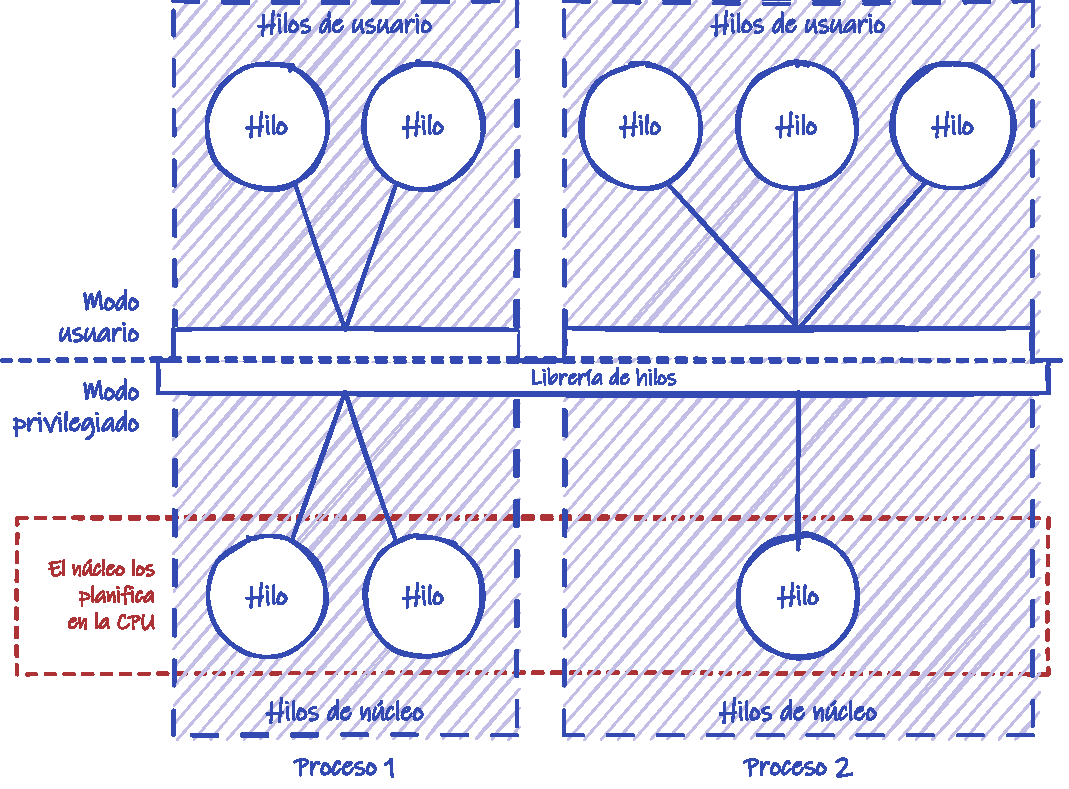
\includegraphics[width=0.8\textwidth]{media/C12_hilos/modelo_muchos_a_muchos.pdf}
\caption{Modelo muchos a muchos
(M:N).}\label{fig-modelo-muchos-a-muchos}
\end{figure}

\subsubsection{Activación del
planificador}\label{_activaciuxf3n_del_planificador}

En el modelo \textbf{muchos a muchos} es conveniente que exista cierto
grado de coordinación entre el núcleo y la \textbf{librería de hilos}
del espacio de usuario. Dicha comunicación tiene como objeto ajustar
dinámicamente el número de \textbf{hilos de núcleo} para garantizar la
máxima eficiencia.

\begin{figure}
\centering
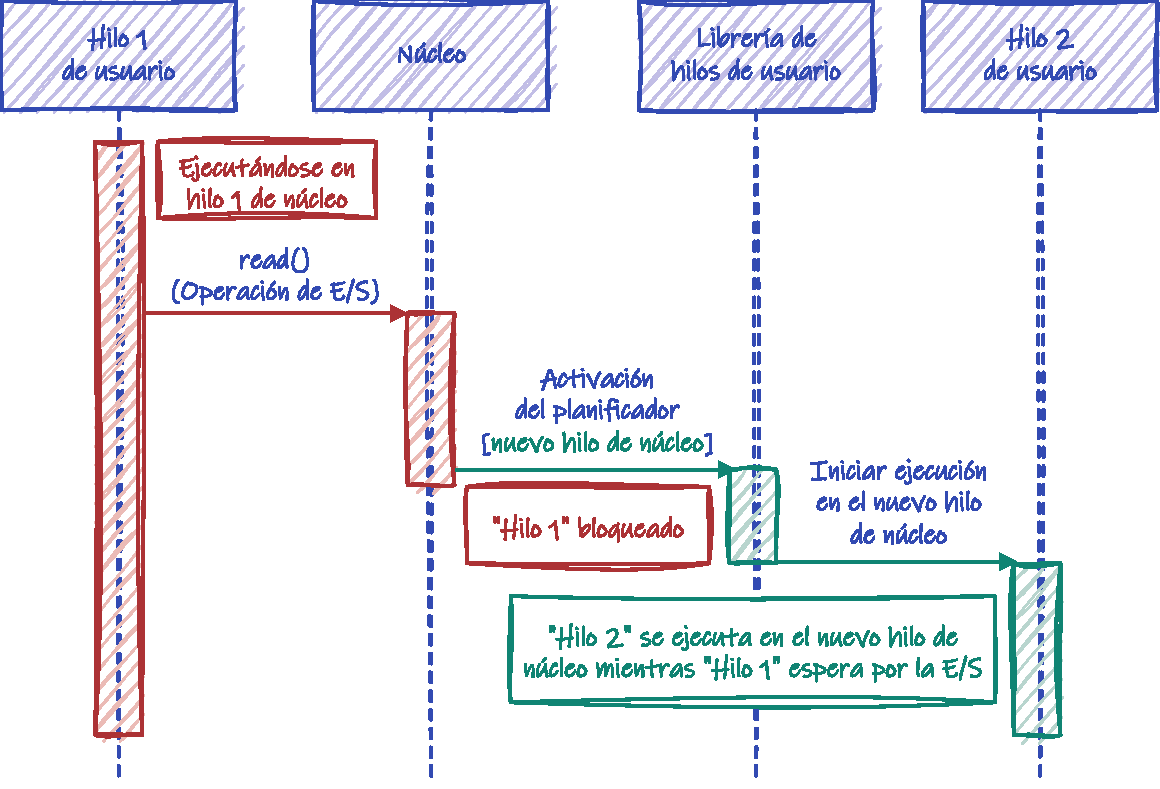
\includegraphics[width=0.8\textwidth]{media/C12_hilos/activación_del_planificador.pdf}
\caption{Diagrama de secuencia del mecanismo de activación del
planificador.}\label{fig-activaciuxf3n-del-planificador}
\end{figure}

Uno de los esquemas de comunicación se denomina \textbf{{}activación del
planificador} y consiste en que el núcleo informa a la \textbf{librería
de hilos} en espacio de usuario que una llamada al sistema, realizada
por uno de sus hilos de usuario, va a bloquear un \textbf{hilo de
núcleo} del proceso cuyos hilos gestiona. Antes de dicha notificación,
el núcleo se encarga de crear un nuevo \textbf{hilo de núcleo} en el
proceso y se lo pasa a la \textbf{librería de hilos} en la notificación
(véase la \hyperref[fig-activaciuxf3n-del-planificador]{Diagrama de
secuencia del mecanismo de activación del planificador.}). Así, el
planificador de la librería puede asignarle alguno de los otros
\textbf{hilos de usuario}, evitando el bloqueo completo del proceso si
no quedan \textbf{hilos de núcleo} disponibles, y ajustando el número de
\textbf{hilos de núcleo} dinámicamente, según las necesidades

\subsubsection{Ventajas e
inconvenientes}\label{_ventajas_e_inconvenientes_3}

Las principales \textbf{ventajas} de este modelo son:

\begin{itemize}
\item
  Permite paralelismo en sistemas multiprocesador, ya que diferentes
  \textbf{hilos de núcleo} pueden ser planificados en distintos
  procesadores y en cada uno puede ejecutarse cualquier \textbf{hilo de
  usuario} de su proceso.
\item
  Permite a otro \textbf{hilo de usuario} del mismo proceso ejecutarse
  cuando un hilo hace una llamada al sistema que debe bloquearse. Si
  esto ocurre el correspondiente hilo de núcleo se queda bloqueado, pero
  el resto de los \textbf{hilos de usuario} pueden seguir ejecutándose
  en los otros \textbf{hilos de núcleo} del proceso (véase el
  \hyperref[_activaciuxf3n_del_planificador]{Activación del
  planificador}).
\end{itemize}

Mientras que el principal \textbf{inconveniente} es su complejidad para
implementarlo y la dificultad de coordinar el planificador de la
librería de hilos en espacio de usuario con el planificador de la CPU
para obtener el mejor rendimiento.

Como veremos en el \hyperref[planificaciuxf3n_de_la_cpu]{???}, los
planificadores de la CPU modernos intentan clasificar los \textbf{hilos
de núcleo} para ordenarlos de la forma más óptima en el acceso a la CPU.
Por ejemplo, no es lo mismo una tarea de cálculo, que necesita usar
intensivamente la CPU, que copia datos de la red o del sistema de
archivos. Generalmente, primero se planifican las segundas, dejando para
el final las tareas intensivas en el uso de la CPU.

En el modelo \textbf{muchos a muchos} un mismo \textbf{hilo de núcleo}
se pueden ejecutar diferentes \textbf{hilos de usuario} que pueden ser
de distinto tipo. Por tanto, cualquier clasificación que haga el
planificador de la CPU puede ser incorrecta en cuanto la
\textbf{librería de hilos} en espacio de usuario cambie el \textbf{hilo
de usuario} que se está ejecutando un \textbf{hilo de núcleo} por otro
diferente. La solución a este problema pasa porque la \textbf{librería
de hilos} en espacio de usuario y el planificador de la CPU intercambien
información sobre sus hilos y se coordinen.

Debido a estas dificultades, muchos sistemas actuales han optado
finalmente por el modelo \textbf{uno a uno}, concentrando esfuerzos en
reducir el coste de creación de \textbf{hilos a nivel de núcleo}, con el
objeto de que haya poca ventaja en implementar también \textbf{hilos a
nivel de usuario}.

Esto no significa que actualmente no se puedan obtener las ventajas del
modelo \textbf{muchos a muchos} en casos en los que puede ser
beneficioso. Para esos casos los desarrolladores pueden utilizar
librerías o lenguajes específicos, con implementaciones diseñadas para
crear un gran número de \textbf{hilos de usuario} con un coste mínimo,
sobre la librería de hilos de los sistemas operativos actuales.

\subsubsection{Implementaciones}\label{_implementaciones_4}

Este modelo se soportaba en sistemas \{freebsd\} y versiones antiguas de
\{netbsd\}, así como en UNIX comerciales, como: \{solaris\} 8 y
anteriores, \{irix\}, \{hpux\} y \{tru64\}. Microsoft Windows también
soportaba este modelo ---a partir de Windows 7 y hasta Windows 10---
gracias a incorporar un mecanismo denominado \emph{planificación en modo
usuario}\hyperref[Win32-UserModeScheduling]{???}.

Algunos lenguajes de programación implementan el modelo \textbf{muchos a
muchos} sobre el modelo \textbf{uno a uno} soportado por la mayoría de
sistemas operativos modernos. Ese es el caso de \{golang\},
\href{https://es.wikipedia.org/wiki/Erlang}{Erlang},
\href{https://es.wikipedia.org/wiki/Elixir_(lenguaje_de_programaci\%C3\%B3n)}{Elixir}
y
\href{https://blogs.oracle.com/javamagazine/post/java-loom-virtual-threads-platform-threads}{Java}.

\subsection{Dos niveles}\label{_dos_niveles}

Existe una variación del modelo \textbf{muchos a muchos} donde, además
de funcionar de la forma comentada anteriormente, se permite que un
\textbf{hilo de usuario} quede ligado indefinidamente a un único
\textbf{hilo de núcleo}, como en el modelo \textbf{uno a uno}.

Esta variación se denomina, en ocasiones, modelo de \textbf{dos niveles}
(véase la \hyperref[fig-modelo-de-dos-niveles]{Modelo de dos niveles.}).

\begin{figure}
\centering
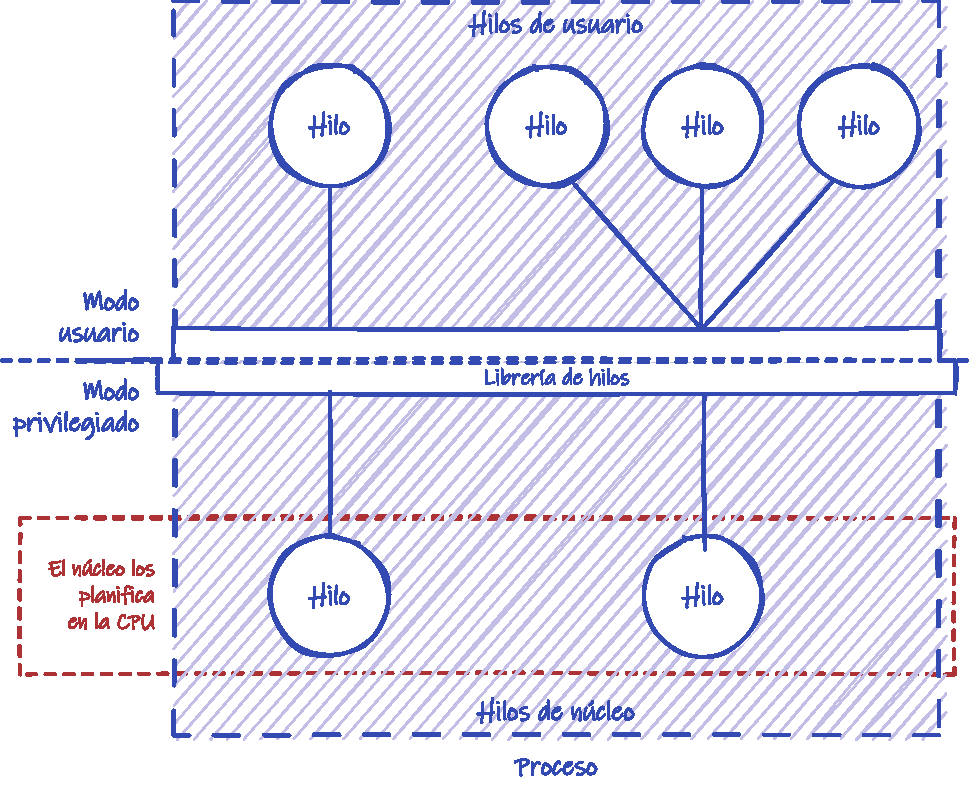
\includegraphics[width=0.8\textwidth]{media/C12_hilos/modelo_de_dos_niveles.pdf}
\caption{Modelo de dos niveles.}\label{fig-modelo-de-dos-niveles}
\end{figure}

\subsubsection{Ventajas e
inconvenientes}\label{_ventajas_e_inconvenientes_4}

El modelo de \textbf{dos niveles} presenta los mismos inconvenientes que
el modelo \textbf{muchos a muchos}, con algunas \textbf{ventajas} en
casos de uso concretos:

\begin{itemize}
\item
  Al vincular un \textbf{hilo de usuario} a un \textbf{hilo de núcleo}
  se asegura la disponibilidad del recurso, lo que puede ser interesante
  si un \textbf{hilo de usuario} es particularmente importante para el
  rendimiento de la aplicación.
\item
  En sistemas con múltiples procesadores o núcleos, puede interesar que
  un \textbf{hilo de usuario} se ejecute siempre en el mismo procesador
  o núcleo para aprovechar la caché y mejorar el rendimiento. Al
  vincular un \textbf{hilo de usuario} a un \textbf{hilo de núcleo} y
  configurar este último para que siempre se planifique en el mismo
  procesador, se está asegurando esta misma condición para el
  \textbf{hilo de usuario} correspondiente.
\end{itemize}

\subsection{El coste de crear hilos y la elección de
modelo}\label{_el_coste_de_crear_hilos_y_la_elecciuxf3n_de_modelo}

Hemos comentado que el modelo \textbf{muchos a uno} debe ser,
teóricamente, «más ligero» que el modelo \textbf{uno a uno}. También
hemos dicho que el modelo \textbf{muchos a muchos}, teóricamente,
permite conservar esa ventaja, al tiempo que ofrece los beneficios del
modelo \textbf{uno a uno}, en lo que respecta al aprovechamiento de los
sistemas multiprocesador. Sin embargo, debemos tener en cuenta que la
diferencia real puede variar en función de múltiples factores.

Un criterio común hasta la década de los 2000, era que el modelo
\textbf{uno a uno} era adecuado hasta varias decenas hilos ---a lo sumo,
en torno a 100 o, quizás, a unos pocos cientos de hilos--- por proceso,
mientras que el modelo \textbf{muchos a uno} podía llegar a varios miles
de hilos.

La principal limitación en la cantidad de \textbf{hilos de usuario} del
modelo \textbf{muchos a uno} estaba en el tamaño del espacio de
direcciones del proceso. Por ejemplo, en las versiones de Windows de 32
bits, los procesos dispone de 2 GiB de su espacio de direcciones para
código y datos. Como cada \emph{fibra} ---que es como se llama a los
hilos del modelo multihilo \textbf{muchos a uno} que implementa la API
Win32 de Windows--- necesita 1 MiB de memoria para su pila, el límite
teórico era de 2048 \emph{fibras}. Este límite era realmente algo
inferior porque en el mismo espacio se almacena el código y los datos
del programa y las librerías que este utiliza.

Una forma de soslayar este problema es indicar al sistema que reserve
menos memoria para la pila al crear cada \emph{fibra}. Esta posibilidad
la suelen soportar los sistemas operativos, independientemente del
modelo multihilo. En el caso de Microsoft Windows, esto permite llegar
hasta cerca de las 32 KiB \emph{fibras} en sistemas de 32 bits.

Posteriormente, se optimizó la creación de \textbf{hilos a nivel de
núcleo}, hasta el punto de equiparar, en gran medida, el coste de cada
hilo en ambos modelos. Mientras que el pasar a sistemas de 64 bits,
permitió superar las limitaciones derivadas por el pequeño tamaño del
espacio de direcciones de los procesos en los sistemas de 32 bits, que
limitaba a ambos modelos multihilo

Actualmente, la creación de \textbf{hilos a nivel de núcleo} se ha
optimizado hasta el punto de que usando el modelo \textbf{uno a uno} se
puede llegar a decenas o cientos de miles de hilos por proceso,
equiparándose a muchas implementaciones del modelo \textbf{muchos a
uno}.

Con suficiente memoria y ajustando el tamaño de la pila de los hilos, se
puede llegar a millones de hilos en ambos modelos. Sin embargo, cuando
se tienen requisitos tan específicos, suele recomendarse utilizar
librerías o lenguajes específicos, con implementaciones concretas del
modelo \textbf{muchos a uno} o \textbf{muchos a muchos} ---siendo
actualmente más interesante porque permite aprovechar el paralelismo de
las CPU modernas--- específicamente diseñadas para escalar hasta dicha
cantidad de hilos.

Algunas de estas implementaciones son:

\begin{itemize}
\item
  \textbf{\{stackless\_python\}}, una implementación del modelo muchos a
  uno para Python. Permite crear un millón de \textbf{hilos a nivel de
  usuario} ---llamados \emph{tasklets}--- consumiendo solo 100 MiB de
  memoria.
\item
  \textbf{\{golang\}}, un lenguaje de programación orientado a la
  creación de servicios de alto rendimiento, que incluye su propia
  implementación del modelo \textbf{muchos a muchos}. Go puede crear un
  millón de \textbf{hilos a nivel de usuario} ---llamadas
  \emph{gorutinas}--- 10 veces más rápido de lo que se pueden crear la
  misma cantidad de hilos del sistema operativo en
  Linux\hyperref[Hansen2023]{???}, utilizando 2 GiB de memoria para las
  pilas.
\item
  \textbf{Java}, soporta
  \href{https://blogs.oracle.com/javamagazine/post/java-loom-virtual-threads-platform-threads}{hilos
  virtuales} ---a partir de la versión 19 como \emph{feature preview}---
  una implementación del modelo \textbf{muchos a muchos}, dirigida a
  cargas de trabajo que necesitan una cantidad extremadamente alta de
  hilos.
\end{itemize}

\section{Operaciones sobre los
hilos}\label{_operaciones_sobre_los_hilos}

Como ocurre con los procesos, es necesario que los hilos pueden ser
creados y eliminados dinámicamente, por lo que los sistemas operativos
deben proporcionar servicios para la creación y cancelación de los
mismos.

\subsection{Creación de hilos}\label{_creaciuxf3n_de_hilos}

En un sistema operativo con librería de hilos implementada en el núcleo,
todo proceso se crea con un hilo, denominado \textbf{hilo principal}{}.
Este es con el que comienza a ejecutarse el programa al entrar en
\{clang\_main\} y el que provoca la terminación de todo el proceso
---incluida la terminación de los otros hilos que existan--- al retornar
de dicha función.

El \textbf{hilo principal} puede crear otros hilos y estos, a su vez,
crear los hilos que necesiten. Pero, a diferencia de lo que ocurre con
los procesos, no existe una relación de padres a hijos ni se crea un
árbol de hilos. Excepto por la característica especial del \textbf{hilo
principal} de que su finalización significa la terminación del proceso,
todos los hilos son iguales entre sí.

En el \hyperref[ejemplo-thread]{example\_title} se puede ver cómo se usa
\{cpp\_thread\} de la librería estándar de C++ para crear hilos.

El código fuente completo de este ejemplo está disponible en
\{threads\_cpp\}. En \{pthreads\_cpp\} se puede ver un ejemplo
equivalente, pero usando \{pthreads\} de la librería de sistema POSIX.
En \{threads\_factorial\_cpp\} se puede examinar un ejemplo más
interesante donde los hilos se utilizan para dividir el cálculo del
factorial de un número, con el objetivo de calcularlo en menos tiempo.

\begin{Shaded}
\begin{Highlighting}[]
\DataTypeTok{void}\NormalTok{ thread\_function}\OperatorTok{(}\DataTypeTok{int}\NormalTok{ thread\_id}\OperatorTok{)}  
\OperatorTok{\{}
    \BuiltInTok{std::}\NormalTok{println}\OperatorTok{(} \StringTok{"[Hilo }\SpecialCharTok{\{\}}\StringTok{] Creado"}\OperatorTok{,}\NormalTok{ thread\_id }\OperatorTok{);}
    \ControlFlowTok{for}\OperatorTok{(}\DataTypeTok{int}\NormalTok{ i }\OperatorTok{=} \DecValTok{0}\OperatorTok{;}\NormalTok{ i }\OperatorTok{\textless{}} \DecValTok{10}\OperatorTok{;} \OperatorTok{++}\NormalTok{i}\OperatorTok{)}
    \OperatorTok{\{}
        \CommentTok{// Dormir el hilo para simular que hace trabajo}
        \CommentTok{// ...}
    \OperatorTok{\}}
\OperatorTok{\}}

\DataTypeTok{int}\NormalTok{ main}\OperatorTok{()}
\OperatorTok{\{}
    \CommentTok{// Crear 3 hilos dentro del proceso}
    \BuiltInTok{std::}\NormalTok{thread thread1}\OperatorTok{(}\NormalTok{ thread\_function}\OperatorTok{,} \DecValTok{1} \OperatorTok{);}   
    \BuiltInTok{std::}\NormalTok{thread thread2}\OperatorTok{(}\NormalTok{ thread\_function}\OperatorTok{,} \DecValTok{2} \OperatorTok{);}
    \BuiltInTok{std::}\NormalTok{thread thread3}\OperatorTok{(}\NormalTok{ thread\_function}\OperatorTok{,} \DecValTok{3} \OperatorTok{);}

    \BuiltInTok{std::}\NormalTok{println}\OperatorTok{(} \StringTok{"[Main] Hilo 1 {-} Id: }\SpecialCharTok{\{\}}\StringTok{, Manejador del sistema: 0x}\SpecialCharTok{\{:x\}}\StringTok{"}\OperatorTok{,}
\NormalTok{        thread1}\OperatorTok{.}\NormalTok{get\_id}\OperatorTok{(),}           
\NormalTok{        thread1}\OperatorTok{.}\NormalTok{native\_handle}\OperatorTok{()} \OperatorTok{);}  

    \CommentTok{// ...}

\NormalTok{    thread1}\OperatorTok{.}\NormalTok{join}\OperatorTok{();} 
\NormalTok{    thread2}\OperatorTok{.}\NormalTok{join}\OperatorTok{();}
\NormalTok{    thread3}\OperatorTok{.}\NormalTok{join}\OperatorTok{();}

    \ControlFlowTok{return}\NormalTok{ EXIT\_SUCCESS}\OperatorTok{;}
\OperatorTok{\}}
\end{Highlighting}
\end{Shaded}

\begin{itemize}
\item
  En C++ se usa la clase \{cpp\_thread\} para crear hilos. Los objetos
  \{cpp\_thread\} no son los hilos sino objetos que sirven para
  gestionar hilos creados en el sistema.
\item
  Todo hilo tiene una función principal que será donde comience la
  ejecución del hilo y que se debe indicar como primer argumento al
  crear el objeto \{cpp\_thread\}. Cuando esa función termine, el hilo
  finalizará.
\item
  Los hilos pueden recibir varios argumentos. Se indican como argumentos
  adicionales al crear el objeto \{cpp\_thread\}, tras el argumento de
  la función principal del hilo. Se pueden usar argumentos pasados por
  referencia o punteros, cuando se quiere usar dichos argumentos para
  devolver resultados.
\item
  Cada objeto \{cpp\_thread\} guarda un identificador del hilo. Este
  identificador no tiene que tener ninguna relación con los
  identificadores o manejadores utilizados por el sistema operativo para
  gestionar los hilos.
\item
  El método \{cpp\_thread\_native\_handle\} permite obtener el manejador
  del sistema operativo del hilo gestionado por ese objeto
  \{cpp\_thread\} en concreto.
\item
  El hilo que invoca \{cpp\_thread\_join\} se queda dormido ---en este
  caso, el hilo principal--- hasta que el hilo indicado en el primer
  argumento termine. Si el hilo principal sale de \{clang\_main\} sin
  esperar a que todos los hilos del proceso terminen, C++ lanza una
  excepción y el programa termina inesperadamente.
\end{itemize}

En los sistemas POSIX, \{cpp\_thread\} se implementa usando la librería
del sistema \{pthreads\}, mientras que en los sistemas Microsoft Windows
utiliza la API Win32. En el \hyperref[ejemplo-pthread]{example\_title}
se puede ver código equivalente al del
\hyperref[ejemplo-thread]{example\_title} pero usando directamente la
API de \{pthreads\}.

El código fuente completo de este ejemplo está disponible en
\{pthreads\_cpp\}. En \{pthreads\_factorial\_cpp\} se puede estudiar un
ejemplo similar, pero dónde se usan los hilos para dividir el cálculo
del factorial de un número.

\begin{Shaded}
\begin{Highlighting}[]
\KeywordTok{struct}\NormalTok{ thread\_args }
\OperatorTok{\{}
    \DataTypeTok{int}\NormalTok{ id}\OperatorTok{;}
    \DataTypeTok{int}\NormalTok{ result}\OperatorTok{;}
\OperatorTok{\};}

\DataTypeTok{void}\OperatorTok{*}\NormalTok{ thread\_function}\OperatorTok{(}\DataTypeTok{void}\OperatorTok{*}\NormalTok{ arg}\OperatorTok{)}   
\OperatorTok{\{}
\NormalTok{    thread\_args}\OperatorTok{*}\NormalTok{ args }\OperatorTok{=} \KeywordTok{static\_cast}\OperatorTok{\textless{}}\NormalTok{thread\_args}\OperatorTok{*\textgreater{}(}\NormalTok{arg}\OperatorTok{);} 

    \BuiltInTok{std::}\NormalTok{println}\OperatorTok{(} \StringTok{"[Hilo }\SpecialCharTok{\{\}}\StringTok{] Creado. Manejador del sistema: 0x}\SpecialCharTok{\{:x\}}\StringTok{"}\OperatorTok{,}
\NormalTok{        args}\OperatorTok{{-}\textgreater{}}\NormalTok{id}\OperatorTok{,}\NormalTok{ pthread\_self}\OperatorTok{()} \OperatorTok{);} 

    \ControlFlowTok{for}\OperatorTok{(}\DataTypeTok{int}\NormalTok{ i }\OperatorTok{=} \DecValTok{0}\OperatorTok{;}\NormalTok{ i }\OperatorTok{\textless{}} \DecValTok{5}\OperatorTok{;} \OperatorTok{++}\NormalTok{i}\OperatorTok{)}
    \OperatorTok{\{}
        \CommentTok{// Dormir el hilo para simular que hace trabajo}
        \CommentTok{// ...}
    \OperatorTok{\}}

\NormalTok{    args}\OperatorTok{{-}\textgreater{}}\NormalTok{result }\OperatorTok{=}\NormalTok{ args}\OperatorTok{{-}\textgreater{}}\NormalTok{id}\OperatorTok{;}
    \ControlFlowTok{return} \OperatorTok{\&}\NormalTok{args}\OperatorTok{{-}\textgreater{}}\NormalTok{result}\OperatorTok{;} 
\OperatorTok{\}}

\DataTypeTok{int}\NormalTok{ main}\OperatorTok{()}
\OperatorTok{\{}
    \DataTypeTok{int}\NormalTok{ return\_code }\OperatorTok{=} \DecValTok{0}\OperatorTok{;}
    \DataTypeTok{pthread\_t}\NormalTok{ thread1}\OperatorTok{,}\NormalTok{ thread2}\OperatorTok{,}\NormalTok{ thread3}\OperatorTok{;}  

\NormalTok{    thread\_args thread1\_args }\OperatorTok{\{} \OperatorTok{.}\NormalTok{id }\OperatorTok{=} \DecValTok{1} \OperatorTok{\};}
\NormalTok{    thread\_args thread2\_args }\OperatorTok{\{} \OperatorTok{.}\NormalTok{id }\OperatorTok{=} \DecValTok{2} \OperatorTok{\};}
\NormalTok{    thread\_args thread3\_args }\OperatorTok{\{} \OperatorTok{.}\NormalTok{id }\OperatorTok{=} \DecValTok{3} \OperatorTok{\};}

    \DataTypeTok{int}\NormalTok{ return\_code }\OperatorTok{=}\NormalTok{ pthread\_create}\OperatorTok{(} 
        \OperatorTok{\&}\NormalTok{thread1}\OperatorTok{,}           
        \KeywordTok{nullptr}\OperatorTok{,}            
\NormalTok{        thread\_function}\OperatorTok{,}    
        \OperatorTok{\&}\NormalTok{thread1\_args }\OperatorTok{);}    

    \ControlFlowTok{if} \OperatorTok{(}\NormalTok{return\_code}\OperatorTok{)} 
    \OperatorTok{\{}
        \BuiltInTok{std::}\NormalTok{println}\OperatorTok{(}\NormalTok{ stderr}\OperatorTok{,} \StringTok{"Error (}\SpecialCharTok{\{\}}\StringTok{) al crear el hilo: }\SpecialCharTok{\{\}}\StringTok{"}\OperatorTok{,}
\NormalTok{            return\_code}\OperatorTok{,} \BuiltInTok{std::}\NormalTok{strerror}\OperatorTok{(}\NormalTok{return\_code}\OperatorTok{)} \OperatorTok{);} 
        \ControlFlowTok{return}\NormalTok{ EXIT\_FAILURE}\OperatorTok{;}
    \OperatorTok{\}}

\NormalTok{    return\_code }\OperatorTok{=}\NormalTok{ pthread\_create}\OperatorTok{(} \OperatorTok{\&}\NormalTok{thread2}\OperatorTok{,} \CommentTok{/* ... */} \OperatorTok{);}
    \ControlFlowTok{if} \OperatorTok{(}\NormalTok{return\_code}\OperatorTok{)}
    \OperatorTok{\{}
        \CommentTok{// ...}
    \OperatorTok{\}}

    \DataTypeTok{int}\OperatorTok{*}\NormalTok{ thread1\_result}\OperatorTok{,} \OperatorTok{*}\NormalTok{thread2\_result}\OperatorTok{,} \OperatorTok{*}\NormalTok{thread3\_result}\OperatorTok{;}

\NormalTok{    pthread\_join}\OperatorTok{(} 
\NormalTok{        thread1}\OperatorTok{,}
        \KeywordTok{reinterpret\_cast}\OperatorTok{\textless{}}\DataTypeTok{void}\OperatorTok{**\textgreater{}(\&}\NormalTok{thread1\_result}\OperatorTok{)} \OperatorTok{);} 
\NormalTok{    pthread\_join}\OperatorTok{(}\NormalTok{ thread2}\OperatorTok{,} \KeywordTok{reinterpret\_cast}\OperatorTok{\textless{}}\DataTypeTok{void}\OperatorTok{**\textgreater{}(\&}\NormalTok{thread2\_result}\OperatorTok{)} \OperatorTok{);}
\NormalTok{    pthread\_join}\OperatorTok{(}\NormalTok{ thread3}\OperatorTok{,} \KeywordTok{reinterpret\_cast}\OperatorTok{\textless{}}\DataTypeTok{void}\OperatorTok{**\textgreater{}(\&}\NormalTok{thread3\_result}\OperatorTok{)} \OperatorTok{);}

    \CommentTok{// ...}

    \ControlFlowTok{return}\NormalTok{ EXIT\_SUCCESS}\OperatorTok{;}
\OperatorTok{\}}
\end{Highlighting}
\end{Shaded}

\begin{itemize}
\item
  En \{pthreads\} se usa \{pthread\_create\} para crear hilos. Devuelve
  un manejador de tipo \texttt{pthread\_t} que podemos usar con otras
  funciones de la API para indicar el hilo que queremos gestionar.
\item
  \texttt{pthread\_t} no es el equivalente al PID de los hilos. Si el
  sistema implementa la librería de hilos en el núcleo, por lo general,
  cada hilo tiene un identificador único; pero \{pthreads\} no ofrece
  una forma de obtenerlo.
\item
  La variable \texttt{pthread\_t} se pasa a \{pthread\_create\} como
  puntero para que al retornar contenga el manejador del hilo, si todo
  ha ido bien.
\item
  Si el hilo se puede crear, \{pthread\_create\} devuelve 0. En caso
  contrario devuelve un código de error.
\item
  Los códigos de error son los mismos que hasta ahora veíamos en
  \{linux\_errno\}. Así que podemos llamar a \{linux\_strerror\} pasando
  el valor retornado, para obtener un texto descriptivo del error.
\item
  Es opcional pasar a \{pthread\_create\} una estructura con atributos
  tales como: tamaño y posición de la pila, política y parámetros de
  planificación, entre otros. En este caso, como no estamos interesados,
  pasamos \texttt{nullptr}
\item
  Todo hilo tiene una función principal que será donde comience la
  ejecución del hilo. Cuando esa función termine, el hilo finalizará.
\item
  Los hilos pueden recibir un argumento en la forma de un puntero a
  \texttt{void*}. Si queremos pasar varios argumentos, lo más sencillo
  es crear una estructura y pasar un puntero a esta.
\item
  En este ejemplo definimos \texttt{thread\_args} para pasar los
  argumentos a los hilos y lo pasamos como \texttt{void*} a la función
  principal. Allí hacemos un \emph{typecast} para recuperar el puntero a
  la estructura \texttt{thread\_args} y poder acceder a sus campos.
\item
  En cualquier momento se puede llamar a \{pthread\_self\} para obtener
  el manejador \texttt{pthread\_t} del hilo actual.
\item
  El hilo que invoca \{pthread\_join\} se queda dormido ---en este caso,
  el hilo principal--- hasta que el hilo indicado en el primer argumento
  termine. Si el hilo principal sale de \{clang\_main\} sin esperar a
  que todos los hilos del proceso terminen, estos mueren inmediatamente,
  junto con el proceso.
\item
  El hilo puede retornar un resultado mediante un puntero
  \textquotesingle void*\textquotesingle. Esto se indica en la sentencia
  \texttt{return} de la función principal del hilo o invocando
  \{pthread\_exit\} para terminar.
\item
  La función \{pthread\_join\} acepta un puntero a \texttt{void*} para
  devolver ese valor de retorno al hilo que la invoca.
\end{itemize}

Como los hilos de \{pthreads\} devuelven punteros, es importante no
intentar devolver variables locales, ya que se destruirán cuando el hilo
termine y el punto devuelto no será válido.

Una alternativa es devolver los resultados a través de la estructura
pasada como argumento. Por ejemplo, el campo \texttt{result} de la
estructura \texttt{thread\_args} ofrece una manera más cómoda de obtener
el resultado del trabajo de cada hilo.

\subsection{Cancelación de hilos}\label{_cancelaciuxf3n_de_hilos}

La \textbf{{}cancelación} es la operación de terminar un hilo antes de
que termine su trabajo. Por ejemplo, en un navegador web un hilo se
puede encargar de la interfaz de usuario mientras otros hilos se
encargan de descargar las páginas y las imágenes de la misma. Si el
usuario pulsa el botón \textbf{Cancelar} es necesario que todos los
hilos que intervienen en la descarga sean cancelados.

Esto puede ocurrir de dos maneras:

\begin{itemize}
\item
  En la \textbf{cancelación asíncrona}{} el hilo termina inmediatamente.
  Esto puede causar problemas al no liberarse los recursos reservados en
  el proceso por parte del hilo Por ejemplo, antes de terminar no se
  cierran archivos abiertos ni se libera memoria de los que solo este
  hilo tiene los descriptores de archivo y los punteros,
  respectivamente.

  Además, si el hilo que termina estaba modificando datos que compartía
  con otros hilos, estos cambios podrían quedar a medias. Esto puede
  dejar las estructuras de datos compartidas en un estado inconsistente,
  causando problemas en otros hilos.
\item
  En la \textbf{cancelación en diferido}{} el hilo comprueba
  periódicamente cuando debe terminar. Si no se tiene cuidado, los
  problemas pueden ser similares a los de la \textbf{cancelación
  asíncrona}. La diferencia es que ahora el desarrollador conoce de
  antemano los puntos donde podría terminar el hilo, lo que da una
  oportunidad de introducirlos solo donde sea seguro terminar.
\end{itemize}

Se denomina \textbf{{}fuga de memoria} al error que ocurre cuando un
bloque de memoria reservada no se libera durante la ejecución del
programa. También pueden ocurrir fugas con otros recursos del sistema
operativo, como: archivos, \emph{sockets}, colas de mensajes o regiones
de memoria compartida.

Generalmente ocurre porque se pierden todas las referencias a un
recurso, por lo que ya no hay oportunidad de liberarlo. Por ejemplo,
cuando se cancela un hilo que es el único que tiene algunas referencias,
sin liberar antes esos recursos.

\subsection{Cancelación en POSIX
Threads}\label{_cancelaciuxf3n_en_posix_threads}

En \{pthreads\} un hilo puede solicitar la cancelación de otro hilo
usando \{pthread\_cancel\}.

\begin{Shaded}
\begin{Highlighting}[]
\DataTypeTok{int}\NormalTok{ return\_code }\OperatorTok{=}\NormalTok{ pthread\_cancel}\OperatorTok{(}\NormalTok{thread}\OperatorTok{);}
\end{Highlighting}
\end{Shaded}

El hilo identificado por el manejador \texttt{thread} será cancelado si
está configurado como cancelable. Por defecto todos los hilos son
cancelables, pero eso lo puede cambiar el propio hilo llamando a
\{pthread\_setcancelstate\}:

\begin{Shaded}
\begin{Highlighting}[]
\DataTypeTok{int}\NormalTok{ return\_code }\OperatorTok{=}\NormalTok{ pthread\_setcancelstate}\OperatorTok{(}
\NormalTok{    PTHREAD\_CANCEL\_DISABLE}\OperatorTok{,} 
    \OperatorTok{\&}\NormalTok{oldstate               }
\OperatorTok{);}
\end{Highlighting}
\end{Shaded}

\begin{itemize}
\item
  Con \texttt{PTHREAD\_CANCEL\_DISABLE} se desactiva la cancelación en
  el hilo que llama la función. El otro valor posible es
  \texttt{PTHREAD\_CANCEL\_ENABLE}.
\item
  La función devuelve a través de un puntero a \texttt{int} el valor
  anterior del estado de cancelación.
\end{itemize}

El tipo de cancelación se puede configurar con
\{pthread\_setcanceltype\}:

\begin{Shaded}
\begin{Highlighting}[]
\DataTypeTok{int}\NormalTok{ return\_code }\OperatorTok{=}\NormalTok{ pthread\_setcanceltypr}\OperatorTok{(}
\NormalTok{    PTHREAD\_CANCEL\_DEFERRED}\OperatorTok{,}    
    \OperatorTok{\&}\NormalTok{oldtype                    }
\OperatorTok{);}
\end{Highlighting}
\end{Shaded}

\begin{itemize}
\item
  Con \texttt{PTHREAD\_CANCEL\_DEFERRED} se activa la
  \textbf{cancelación en diferido}, que de todas formas es el tipo de
  cancelación por defecto. El otro valor posible es
  \texttt{PTHREAD\_CANCEL\_ASYNCHRONOUS}, que corresponde con la
  \textbf{cancelación asíncrona}.
\item
  La función devuelve a través de un puntero a \texttt{int} el valor
  anterior del tipo de cancelación.
\end{itemize}

Se pueden cambiar entre estado y tipo de cancelación en cualquier
momento, según lo que encaje mejor con las características de las
distintas partes del código.

\subsubsection{Cancelación
asíncrona}\label{_cancelaciuxf3n_asuxedncrona}

{} Por los motivos comentados anteriormente, no es recomendable la
\textbf{cancelación asíncrona}, a menos que estemos muy seguros de que
no puede causar problemas. Uno de los pocos casos con los que es
compatible es en bucles 100\% dedicados a ejecutar cálculos en la CPU,
como el siguiente:

\begin{Shaded}
\begin{Highlighting}[]
\DataTypeTok{int}\NormalTok{ factorial }\OperatorTok{=} \DecValTok{1}\OperatorTok{;}
\ControlFlowTok{for} \OperatorTok{(} \DataTypeTok{int}\NormalTok{ i }\OperatorTok{=} \DecValTok{2}\OperatorTok{;}\NormalTok{ i }\OperatorTok{\textless{}=}\NormalTok{ number}\OperatorTok{;}\NormalTok{ i}\OperatorTok{++} \OperatorTok{)}
\OperatorTok{\{}
\NormalTok{    factorial }\OperatorTok{=}\NormalTok{ factorial }\OperatorTok{*}\NormalTok{ i}\OperatorTok{;}
\OperatorTok{\}}
\end{Highlighting}
\end{Shaded}

La \textbf{cancelación asíncrona} no se debe usar si el código reserva
memoria dinámicamente o solicita otros recursos del sistema operativo,
porque el hilo podría terminar en cualquier momento sin liberarlos.
Tampoco si se modifican estructuras de datos, porque los cambios pueden
quedar a medias.

Por ejemplo, si la cancelación ocurre en medio de una llamada a
\{clang\_malloc\} o \{cpp\_new\} no hay forma de saber si ocurrió antes
de que la memoria fuera reservada o después. Incluso puede haber
ocurrido en medio de la operación, dejando en estado inconsistente las
estructuras de datos que sirven para seguir la pista de las zonas de
memoria reservadas y libres.

El estándar POSIX solo indica que las funciones
\{pthread\_setcancelstate\} y \{pthread\_setcanceltype\} deben ser
seguras frente a la \textbf{cancelación asíncrona} del hilo. En general,
no se puede llamar a otras funciones de la librería del sistema de forma
segura en un hilo cancelable asíncronamente.

\subsubsection{Cancelación en
diferido}\label{_cancelaciuxf3n_en_diferido}

{} Por tanto, la \textbf{cancelación en diferido} es la mejor
alternativa. Con este tipo de cancelación, la terminación del hilo
ocurre en puntos concretos del código.

En la terminología de \{pthreads\} a estos puntos se los denomina
\textbf{puntos de cancelación}{} y la inmensa mayoría de las llamadas al
sistema que puede poner el hilo en estado \textbf{esperando} lo son por
sí mismas. Por ejemplo, \{linux\_open\}, \{linux\_close\},
\{linux\_read\}, \{linux\_write\}, \{linux\_recv\}, \{linux\_send\},
\{linux\_poll\} y \{linux\_sleep\}, entre muchas otras (véase la lista
en la sección «\emph{Cancellation points}» de la documentación de
\{pthreads\}). Eso significa que seguramente también sean \textbf{puntos
de cancelación}, las funciones de la librería del sistema y de la
librería estándar del lenguaje que utilizan esas llamadas al sistema.

Sabiendo esto, se puede estudiar cada caso. Si no es seguro permitir la
cancelación de un hilo en la invocación de una de estas funciones en
nuestro código, se puede usar \{pthread\_setcancelstate\} para
desactivar temporalmente el mecanismo de cancelación. Por ejemplo, una
llamada a \{clang\_printf\} como ayuda para depurar, en medio de los
pasos para modificar una estructura de datos ---como una lista enlazada
o una cola--- introduce un \textbf{punto de cancelación} en lugar poco
seguro; porque si el hilo se cancela en ese punto, la estructura de
datos quedará en estado inconsistente. La solución es eliminar la
llamada a \{clang\_printf\} o desactivar temporalmente el mecanismo de
cancelación.

De forma inversa, se pueden introducir manualmente puntos de cancelación
llamando a \{pthread\_testcancel\}. Por ejemplo, el siguiente bucle no
hace llamadas al sistema, por lo que no tiene puntos de cancelación:

\begin{Shaded}
\begin{Highlighting}[]
\DataTypeTok{int}\NormalTok{ factorial }\OperatorTok{=} \DecValTok{1}\OperatorTok{;}
\ControlFlowTok{for} \OperatorTok{(} \DataTypeTok{int}\NormalTok{ i }\OperatorTok{=} \DecValTok{2}\OperatorTok{;}\NormalTok{ i }\OperatorTok{\textless{}=}\NormalTok{ number}\OperatorTok{;}\NormalTok{ i}\OperatorTok{++} \OperatorTok{)}
\OperatorTok{\{}
\NormalTok{    factorial }\OperatorTok{=}\NormalTok{ factorial }\OperatorTok{*}\NormalTok{ i}\OperatorTok{;}
\OperatorTok{\}}
\end{Highlighting}
\end{Shaded}

Eso significa que ese código para calcular el factorial de
\texttt{number} podría ejecutarse durante bastante tiempo sin ofrecer
una oportunidad para cancelar el hilo; incluso aunque es un código muy
seguro desde el punto de vista de la cancelación. La solución es
introducir manualmente un punto de cancelación:

\begin{Shaded}
\begin{Highlighting}[]
\DataTypeTok{int}\NormalTok{ factorial }\OperatorTok{=} \DecValTok{1}\OperatorTok{;}
\ControlFlowTok{for} \OperatorTok{(} \DataTypeTok{int}\NormalTok{ i }\OperatorTok{=} \DecValTok{2}\OperatorTok{;}\NormalTok{ i }\OperatorTok{\textless{}=}\NormalTok{ number}\OperatorTok{;}\NormalTok{ i}\OperatorTok{++} \OperatorTok{)}
\OperatorTok{\{}
\NormalTok{    factorial }\OperatorTok{=}\NormalTok{ factorial }\OperatorTok{*}\NormalTok{ i}\OperatorTok{;}
\NormalTok{    pthread\_testcancel}\OperatorTok{();}   
\OperatorTok{\}}
\end{Highlighting}
\end{Shaded}

\begin{itemize}
\item
  Comprobar si se ha solicitado la cancelación del hilo y si es así,
  cancelar el hilo.
\end{itemize}

La \textbf{cancelación en diferido} también presenta retos desde el
punto de vista de evitar las fugas de memoria y de otros recursos cuando
un hilo es cancelado. Por ejemplo, supongamos que tenemos una función
que abre una tubería, crea un hilo para gestionar los mensajes que
llegan y devuelve un puntero a una estructura de datos que se puede usar
en otras funciones de la librería ---de forma similar a \{clang\_fopen\}
y \texttt{FILE*}---:

\begin{Shaded}
\begin{Highlighting}[]
\NormalTok{CONN}\OperatorTok{*}\NormalTok{ conn\_open}\OperatorTok{(} \CommentTok{/* ... */} \OperatorTok{)}
\OperatorTok{\{}
\NormalTok{    CONN}\OperatorTok{*}\NormalTok{ handler }\OperatorTok{=}\NormalTok{ malloc}\OperatorTok{(} \KeywordTok{sizeof}\OperatorTok{(}\NormalTok{CONN}\OperatorTok{)} \OperatorTok{);}
    \ControlFlowTok{if}\OperatorTok{(}\NormalTok{handler }\OperatorTok{==}\NormalTok{ NULL}\OperatorTok{)}
    \OperatorTok{\{}
        \ControlFlowTok{return}\NormalTok{ NULL}\OperatorTok{;}
    \OperatorTok{\}}

\NormalTok{    handler}\OperatorTok{{-}\textgreater{}}\NormalTok{fifofd }\OperatorTok{=}\NormalTok{ open}\OperatorTok{(} \CommentTok{/* ... */} \OperatorTok{);}
    \ControlFlowTok{if} \OperatorTok{(}\NormalTok{fifofd }\OperatorTok{\textless{}} \DecValTok{0}\OperatorTok{)}
    \OperatorTok{\{}
\NormalTok{        free}\OperatorTok{(}\NormalTok{ handler }\OperatorTok{);} 
        \ControlFlowTok{return}\NormalTok{ NULL}\OperatorTok{;}
    \OperatorTok{\}}

    \DataTypeTok{int}\NormalTok{ return\_code }\OperatorTok{=}\NormalTok{ pthread\_create}\OperatorTok{(\&}\NormalTok{handler}\OperatorTok{{-}\textgreater{}}\NormalTok{thread}\OperatorTok{,} \CommentTok{/* ... */}\OperatorTok{,}\NormalTok{ handler }\OperatorTok{);}
    \ControlFlowTok{if} \OperatorTok{(}\NormalTok{return\_code}\OperatorTok{)}
    \OperatorTok{\{}
\NormalTok{        close}\OperatorTok{(}\NormalTok{ handler}\OperatorTok{{-}\textgreater{}}\NormalTok{fifofd }\OperatorTok{);} 
\NormalTok{        free}\OperatorTok{(}\NormalTok{ handler }\OperatorTok{);} 
        \ControlFlowTok{return}\NormalTok{ NULL}\OperatorTok{;}
    \OperatorTok{\}}

    \ControlFlowTok{return}\NormalTok{ handler}\OperatorTok{;}
\OperatorTok{\}}
\end{Highlighting}
\end{Shaded}

\begin{itemize}
\item
  Evitar la \textbf{fuga de memoria} si \{linux\_open\} o
  \{pthread\_create\} fallan.
\item
  Evitar la fuga del \emph{socket} si \{pthread\_create\} falla.
\end{itemize}

Este código y la forma en que maneja los errores funcionan bien en
programas monohilo, porque estamos seguros de que al salir de la función
o se completaron todas las etapas o ninguna. Es decir, si alguna de las
peticiones al sistema falla, las hechas anteriormente se «deshacen» para
evitar la fuga de recursos.

Pero no es correcto en programas multihilo porque \{linux\_open\} y
\{linux\_close\} son \textbf{puntos de cancelación}. Si
\texttt{conn\_open()} es llamada desde un hilo y ese hilo es cancelado,
el hilo podría terminar a mitad de la función, sin liberar
\texttt{handler}, creando una \textbf{fuga de memoria} que no se
liberará hasta que el proceso termine. Si \texttt{conn\_open()} es
llamada en múltiples ocasiones, cada una es una oportunidad para perder
memoria.

El código anterior se puede mejorar usando \textbf{manejadores de
limpieza}{}. Esos manejadores se organizan en una pila de la que se
pueden insertar o extraer llamando a \{pthread\_cleanup\_push\} y
\{pthread\_cleanup\_pop\}, respectivamente. Cuando el hilo es cancelado,
la librería extrae los manejadores de la pila y los va ejecutando en
orden, antes de terminar.

\begin{Shaded}
\begin{Highlighting}[]
\NormalTok{CONN}\OperatorTok{*}\NormalTok{ conn\_open}\OperatorTok{(} \CommentTok{/* ... */} \OperatorTok{)}
\OperatorTok{\{}
\NormalTok{    CONN}\OperatorTok{*}\NormalTok{ handler }\OperatorTok{=}\NormalTok{ malloc}\OperatorTok{(} \KeywordTok{sizeof}\OperatorTok{(}\NormalTok{CONN}\OperatorTok{)} \OperatorTok{);}
    \ControlFlowTok{if}\OperatorTok{(}\NormalTok{handler }\OperatorTok{==}\NormalTok{ NULL}\OperatorTok{)}
    \OperatorTok{\{}
        \ControlFlowTok{return}\NormalTok{ NULL}\OperatorTok{;}
    \OperatorTok{\}}

\NormalTok{    pthread\_cleanup\_push}\OperatorTok{(\&}\NormalTok{free}\OperatorTok{,}\NormalTok{ handler}\OperatorTok{);} 

\NormalTok{    handler}\OperatorTok{{-}\textgreater{}}\NormalTok{fifofd }\OperatorTok{=}\NormalTok{ open}\OperatorTok{(} \CommentTok{/* ... */} \OperatorTok{);}  
    \ControlFlowTok{if} \OperatorTok{(}\NormalTok{fifofd }\OperatorTok{\textless{}} \DecValTok{0}\OperatorTok{)}
    \OperatorTok{\{}
\NormalTok{        pthread\_cleanup\_pop}\OperatorTok{(}\DecValTok{1}\OperatorTok{);}     \CommentTok{// free(handler) }
        \ControlFlowTok{return}\NormalTok{ NULL}\OperatorTok{;}
    \OperatorTok{\}}

\NormalTok{    pthread\_cleanup\_push}\OperatorTok{(\&}\NormalTok{cleanup\_fd}\OperatorTok{,} \OperatorTok{\&}\NormalTok{handler}\OperatorTok{{-}\textgreater{}}\NormalTok{fifofd}\OperatorTok{);}

    \DataTypeTok{int}\NormalTok{ return\_code }\OperatorTok{=}\NormalTok{ pthread\_create}\OperatorTok{(\&}\NormalTok{handler}\OperatorTok{{-}\textgreater{}}\NormalTok{thread}\OperatorTok{,} \CommentTok{/* ... */}\OperatorTok{,}\NormalTok{ handler }\OperatorTok{);}
    \ControlFlowTok{if} \OperatorTok{(}\NormalTok{return\_code}\OperatorTok{)}
    \OperatorTok{\{}
\NormalTok{        close}\OperatorTok{(}\NormalTok{ handler}\OperatorTok{{-}\textgreater{}}\NormalTok{fifofd }\OperatorTok{);} 
\NormalTok{        pthread\_cleanup\_pop}\OperatorTok{(}\DecValTok{1}\OperatorTok{);}     \CommentTok{// free(handler) }
        \ControlFlowTok{return}\NormalTok{ NULL}\OperatorTok{;}
    \OperatorTok{\}}

\NormalTok{    pthread\_cleanup\_pop}\OperatorTok{(}\DecValTok{0}\OperatorTok{);} 

    \ControlFlowTok{return}\NormalTok{ handler}\OperatorTok{;}
\OperatorTok{\}}
\end{Highlighting}
\end{Shaded}

\begin{itemize}
\item
  Nada más reservar la memoria de \texttt{CONN} se añade un
  \textbf{manejador de limpieza} que llamará a \texttt{free(handler)} si
  el hilo va a ser cancelado. Así nos aseguramos que \texttt{handler}
  será liberado si el hilo es cancelado.
\item
  La cancelación solo puede ocurrir en los \textbf{puntos de
  cancelación} que son las llamadas a \{linux\_open\} y
  \{linux\_close\}.
\item
  En caso de error, el \textbf{manejador de limpieza} ya no hace falta,
  así que se extrae antes de salir de la función. Se llama a
  \{pthread\_cleanup\_pop\} con valor distinto de 0 porque así la
  función extrae el manejador y lo invoca. A fin de cuentas se sale a
  causa de un error, por lo que sigue siendo necesario ejecutar
  \texttt{free(handler)} para evitar una \textbf{fuga de memoria}.
\item
  Al terminar la función se extraen todos los manejadores de señal,
  puesto que ya no hacen falta. El argumento 0 hace que
  \{pthread\_cleanup\_pop\} no ejecute el manejador de limpieza
  extraído.
\end{itemize}

Ahora \texttt{conn\_open()} maneja correctamente la cancelación del hilo
donde se ejecuta, por lo que puede usarse sin problemas en aplicaciones
multihilo.

\subsection{Cancelación de hilos en lenguajes de alto
nivel}\label{_cancelaciuxf3n_de_hilos_en_lenguajes_de_alto_nivel}

El mecanismo de cancelación de hilos descrito funciona razonablemente
bien en C, pero no con lenguajes de más alto nivel, como C++, Java o
C\#. Las librerías de hilos suelen ser librerías en C, que no conocen
nada de objetos ni de otras particularidades de esos lenguajes.

Por ejemplo, en C++, antes de terminar un hilo, deberían ser llamados
todos los destructores de los objetos locales, para evitar \textbf{fugas
de memoria} y de otros recursos, datos sin escribir y otros problemas
derivados de tener objetos que no se destruyen adecuadamente.
Lamentablemente, el mecanismo de cancelación de \{pthreads\} ---y el de
otras librerías de hilos, como la de Windows API--- no sabe hacer nada
de eso. Cada lenguaje debe implementar su propia solución.

En Java y C\#, por ejemplo, cuando un punto de cancelación detecta una
petición de cancelación emite la excepción \texttt{Thread.Interrupt},
que retrocede por la pila de llamadas, liberando las variables locales
hasta salir por el método principal del hilo. A este mecanismo se lo
denomina \textbf{cancelación coordinada}{}.

En C++ no se ha incluido un mecanismo de cancelación en el estándar
hasta C++20. Antes de C++20, la forma recomendada de implementar la
cancelación es pasando a los hilos una variable de tipo \texttt{bool}
con la que señalarles cuándo deben terminar. El código de los hilos debe
comprobar frecuentemente el valor de dicha variable y, llegado el
momento, terminar retornando ordenadamente por la función principal del
hilo.

En C++20 esta estrategia de \textbf{cancelación cooperativa}{} se ha
formalizado e incluido en el estándar al introducir la clase
\{cpp\_jthread\}. Esta nueva clase de hilo puede pasar a la función
principal lo que se llama un \textbf{{}\emph{token} de cancelación}{}
---en lugar de la variable tipo \texttt{bool} que comentamos
anteriorment--- que se debe comprobar regularmente para saber si hay que
terminar el hilo prematuramente.

En el \hyperref[ejemplo-jthread]{example\_title} se ilustra de forma
simplificada cómo se usa \{cpp\_jthread\} en
\{jthreads\_factorial\_cpp\} para crear hilos para calcular el factorial
de un número, cancelando el cálculo antes de que termine.

El código fuente completo de este ejemplo está disponible en
\{jthreads\_factorial\_cpp\}.

\begin{Shaded}
\begin{Highlighting}[]
\DataTypeTok{int}\NormalTok{ compute\_factorial}\OperatorTok{(}\BuiltInTok{std::}\NormalTok{stop\_token stoken}\OperatorTok{,} \DataTypeTok{int}\NormalTok{ number}\OperatorTok{,} \DataTypeTok{int}\NormalTok{ lower\_bound}\OperatorTok{)} 
\OperatorTok{\{}
\NormalTok{    factorial }\OperatorTok{=} \DecValTok{1}\OperatorTok{;}
    \ControlFlowTok{for} \OperatorTok{(} \DataTypeTok{int}\NormalTok{ i }\OperatorTok{=}\NormalTok{ lower\_bound}\OperatorTok{;}\NormalTok{ i }\OperatorTok{\textless{}=}\NormalTok{ number}\OperatorTok{;}\NormalTok{ i}\OperatorTok{++} \OperatorTok{)}
    \OperatorTok{\{}
        \ControlFlowTok{if}\OperatorTok{(}\NormalTok{stoken}\OperatorTok{.}\NormalTok{stop\_requested}\OperatorTok{())} 
        \OperatorTok{\{}
            \ControlFlowTok{return}\NormalTok{ factorial}\OperatorTok{;}
        \OperatorTok{\}}
\NormalTok{        factorial }\OperatorTok{=}\NormalTok{ factorial }\OperatorTok{*}\NormalTok{ i}\OperatorTok{;}
    \OperatorTok{\}}
\OperatorTok{\}}

\DataTypeTok{void}\NormalTok{ factorial\_thread }\OperatorTok{(}\BuiltInTok{std::}\NormalTok{stop\_token stoken}\OperatorTok{,} \DataTypeTok{int}\OperatorTok{\&}\NormalTok{ result}\OperatorTok{,} \DataTypeTok{int}\NormalTok{ number}\OperatorTok{,} 
    \DataTypeTok{int}\NormalTok{ lower\_bound}\OperatorTok{)}
\OperatorTok{\{}
\NormalTok{    result }\OperatorTok{=}\NormalTok{ cancellable\_calculate\_factorial}\OperatorTok{(}\NormalTok{ stoken}\OperatorTok{,}\NormalTok{ number}\OperatorTok{,}\NormalTok{ lower\_bound }\OperatorTok{);}
\OperatorTok{\}}

\DataTypeTok{int}\NormalTok{ main}\OperatorTok{()}
\OperatorTok{\{}
    \KeywordTok{auto}\NormalTok{ number }\OperatorTok{=} \CommentTok{/* Leer el número de algún sitio */}\OperatorTok{;}

    \CommentTok{// Para calcular el number!, un hilo multiplica desde number a number/2 y el}
    \CommentTok{// otro desde (number/2){-}1 hasta 2.}
    \KeywordTok{auto}\NormalTok{ thread1\_lower\_bound }\OperatorTok{=}\NormalTok{ number }\OperatorTok{/} \DecValTok{2}\OperatorTok{;}
    \KeywordTok{auto}\NormalTok{ thread2\_number }\OperatorTok{=}\NormalTok{ thread1\_lower\_bound }\OperatorTok{{-}} \DecValTok{1}\OperatorTok{;}

    \DataTypeTok{int}\NormalTok{ thread1\_result}\OperatorTok{,}\NormalTok{ thread2\_result}\OperatorTok{;}

    \BuiltInTok{std::}\NormalTok{jthread thread1}\OperatorTok{(}\NormalTok{factorial\_thread}\OperatorTok{,} \BuiltInTok{std::}\NormalTok{ref}\OperatorTok{(}\NormalTok{thread1\_result}\OperatorTok{),}  
\NormalTok{        number}\OperatorTok{,}\NormalTok{ thread1\_lower\_bound}\OperatorTok{);}
    \BuiltInTok{std::}\NormalTok{jthread thread2}\OperatorTok{(}\NormalTok{factorial\_thread}\OperatorTok{,} \BuiltInTok{std::}\NormalTok{ref}\OperatorTok{(}\NormalTok{thread2\_result}\OperatorTok{),}  
\NormalTok{        thread2\_number}\OperatorTok{,} \DecValTok{2}\OperatorTok{);}

    \CommentTok{// ...}

\NormalTok{    thread1}\OperatorTok{.}\NormalTok{request\_stop}\OperatorTok{();} 
\NormalTok{    thread2}\OperatorTok{.}\NormalTok{request\_stop}\OperatorTok{();} 

\NormalTok{    thread1}\OperatorTok{.}\NormalTok{join}\OperatorTok{();} 
\NormalTok{    thread2}\OperatorTok{.}\NormalTok{join}\OperatorTok{();} 

    \CommentTok{// ...}
    
\OperatorTok{\}}
\end{Highlighting}
\end{Shaded}

\begin{itemize}
\item
  Crear e iniciar el hilo con \{cpp\_jthread\} para calcular el
  factorial de \texttt{number}.
\item
  Al crear el hilo, la clase \{cpp\_jthread\} le pasa a la función el
  \textbf{\emph{token} de cancelación} \texttt{stoken}. Este
  \textbf{\emph{token} de cancelación} se debe propagar desde la función
  principal a las funciones cancelables que este hilo invoque.
\item
  En algún momento de la ejecución del programa se pide a los hilos que
  se detengan antes de terminar los cálculos. Un posible motivo es que
  el usuario haya pulsado el botón de cancelar o porque se haya excedido
  el tiempo de cálculo.
\item
  Después de pedir la cancelación, el programa espera a que los hilos
  terminen antes de continuar la ejecución del hilo principal.
\item
  Periódicamente, el código del hilo debe comprobar el
  \textbf{\emph{token} de cancelación}. Si se ha pedido la cancelación,
  se termina el hilo retornando.
\item
  También se puede dejar que la cancelación ocurra automáticamente al
  salir de la función. El destructor de los objetos \{cpp\_jthread\}
  ---a diferencia del de cpp\_thread--- se encarga de pedir la
  cancelación de los hilos, llamando a \{cpp\_jthread\_request\_stop\},
  y luego espera a que terminen usando \{cpp\_jthread\_join\}.
\end{itemize}

Java y C\# han terminado incluyendo también este tipo de
\textbf{cancelación cooperativa} usando un \textbf{\emph{token} de
cancelación}, debido a los problemas que tienen los desarrolladores para
recordar usar correctamente la excepción de la \textbf{cancelación
coordinada}.

\section{Otras consideraciones sobre los
hilos}\label{_otras_consideraciones_sobre_los_hilos}

\subsection{Las llamadas al sistema fork() y exec() en procesos
multihilo}\label{_las_llamadas_al_sistema_fork_y_exec_en_procesos_multihilo}

La llamada al sistema \{linux\_fork\} de los sistemas POSIX es anterior
a la existencia del concepto de \textbf{hilo}. Así que cuando estos
aparecieron surgió el problema de si al llamar a \{linux\_fork\} en un
proceso multihilo:

\begin{itemize}
\item
  El nuevo proceso debía tener un duplicado de todos los hilos.
\item
  O el nuevo proceso debía tener un único hilo copia del que invocó a
  \{linux\_fork\}.
\end{itemize}

Como hemos comentado anteriormente, la llamada al sistema
\{linux\_fork\} sustituye el programa en ejecución con un nuevo programa
e inicia su ejecución en \{clang\_main\}. Esto incluye liberar toda la
memoria reservada y la destrucción de todos los hilos del programa
original, por lo que duplicar los hilos en el proceso hijo creado por
\{linux\_fork\}, si luego se va a llamar a \{linux\_exec\} parece algo
innecesario.

El estándar POSIX establece que si se utiliza \{linux\_fork\} en un
programa multihilo, el nuevo proceso debe ser creado con un solo hilo,
que será una réplica del que hizo la llamada, así como un duplicado
completo del espacio de direcciones del proceso.

Sin embargo, algunos sistemas UNIX tienen una segunda llamada no
estándar denominada \texttt{forkall()}, capaz de duplicar todos los
hilos del proceso padre. Obviamente solo resulta conveniente emplearla
si no se va a utilizar la llamada \{linux\_exec\} a continuación. La
inclusión de \texttt{forkall()} en el estándar POSIX fue considerada y
rechazada.

\subsection{Manejo de señales en procesos
multihilo}\label{_manejo_de_seuxf1ales_en_procesos_multihilo}

En el \hyperref[_seuxf1ales_en_sistemas_operativos_posix]{???} hablamos
del uso de las señales{} como mecanismo de comunicación, pero en general
sirven para informar a un proceso del suceso de ciertos eventos.

Existen dos tipos de señales:

\begin{itemize}
\item
  Las \textbf{señales síncronas}{} se deben a alguna acción del propio
  proceso. Ejemplos de señales de este tipo son \texttt{SIGSEV} y
  \texttt{SIGFE}, originadas por accesos ilegales a memoria o divisiones
  por 0, respectivamente.

  Las señales síncronas son enviadas al mismo proceso que las origina.
\item
  Las \textbf{señales asíncronas}{} son debidas a acciones externas. Un
  ejemplo de este tipo de señales es la terminación de procesos con
  teclas especiales como {CTRL+C} o CTRL-D, que envían al proceso las
  señales \texttt{SIGINT} y \texttt{SIGHUP} respectivamente. También lo
  son las señales enviadas desde otro proceso, como cuando el proceso
  \textbf{init} envía \texttt{SIGTERM} al resto de procesos para
  informales que deben terminar porque el sistema se va a apagar.
\end{itemize}

Como hemos visto, las señales que llegan a un proceso pueden ser
interceptadas por una función definida por el programador llamada
\textbf{manejador de señal}{}.

Las señales también son anteriores a los hilos, por lo que cuando
aparecieron los hilos se tuvieron que tomar decisiones sobre cómo iban a
encajar ambos conceptos. Por ejemplo, decidir cuál de los hilos del
proceso, será interrumpido cuando llegue una señal, para ejecutar el
manejador de señales.

\subsubsection{Señales enviadas por otros
hilos}\label{_seuxf1ales_enviadas_por_otros_hilos}

En los sistemas POSIX multihilo se pueden enviar señales a un proceso:

\begin{Shaded}
\begin{Highlighting}[]
\NormalTok{kill}\OperatorTok{(}\NormalTok{pid}\OperatorTok{,}\NormalTok{ SIGTERM}\OperatorTok{);}
\end{Highlighting}
\end{Shaded}

En ese caso uno cualquiera de los hilos podrá ser interrumpido para
ejecutar el manejador de señal.

Cada hilo puede enmascarar las señales que considere llamando a
\{pthread\_sigmask\} Es decir, cada hilo puede elegir qué señales quiere
bloquear para no tener que atenderlas:

\begin{Shaded}
\begin{Highlighting}[]
\NormalTok{sigset\_t set}\OperatorTok{;}               

\NormalTok{sigemptyset}\OperatorTok{(\&}\NormalTok{set}\OperatorTok{);}          
\NormalTok{sigaddset}\OperatorTok{(\&}\NormalTok{set}\OperatorTok{,}\NormalTok{ SIGINT}\OperatorTok{);}    
\NormalTok{sigaddset}\OperatorTok{(\&}\NormalTok{set}\OperatorTok{,}\NormalTok{ SIGUSR1}\OperatorTok{);}   

\NormalTok{pthread\_sigmask}\OperatorTok{(}\NormalTok{SIG\_BLOCK}\OperatorTok{,} \OperatorTok{\&}\NormalTok{set}\OperatorTok{,}\NormalTok{ NULL}\OperatorTok{);} 
\end{Highlighting}
\end{Shaded}

\begin{itemize}
\item
  Las máscaras de señales se definen mediante \emph{sets} de señales. El
  tipo de los \emph{sets} de señales es \texttt{sigset\_t}, de cuyo tipo
  real no deberíamos preocuparnos, por portabilidad.
\item
  Para manipular los \emph{sets} se proporcionan una serie de funciones.
  \{linux\_sigemptyset\} es para asegurar que el \emph{set} está vacío.
\item
  Añadimos al \emph{set} la señal \texttt{SIGINT}.
\item
  Añadimos al \emph{set} la señal \texttt{SIGINT}.
\item
  Bloqueamos en el hilo actual las señales en el \emph{set}
  \texttt{set},es decir, \texttt{SIGINT} y \texttt{SIGUSR1}.
\end{itemize}

Así una señal enviada a un proceso interrumpirá a uno de los hilos que
no la haya bloqueado.

También se puede enviar una señal a un hilo en concreto usando
\{pthread\_kill\}. El hilo será interrumpido si no la ha bloqueado.

\begin{Shaded}
\begin{Highlighting}[]
\NormalTok{pthread\_kill}\OperatorTok{(}\NormalTok{thread}\OperatorTok{,}\NormalTok{ SIGTERM}\OperatorTok{);}
\end{Highlighting}
\end{Shaded}

Sin embargo, hay que tener en cuenta que el manejo de señales es un
recurso del proceso, compartido por todos sus hilos. Esto quiere decir
que si la señal está configurada para ser manejada usando la acción por
defecto y dicha acción es terminar, terminará todo el proceso, aunque la
señal haya sido dirigida a un hilo en concreto.

\subsubsection{Señales enviadas por el
sistema}\label{_seuxf1ales_enviadas_por_el_sistema}

Lo que queda por ver es a quién va dirigida una señal, cuando es el
sistema quién la envía para notificar un evento:

\begin{itemize}
\item
  Las señales síncronas son causadas por un error en la ejecución, que
  en un proceso multihilo es debido a la fallida ejecución de un hilo en
  particular. Por eso estas señales se dirigen al hilo que las causa.
\item
  Las señales asíncronas llegan por causas externas, así que se dirigen
  al proceso, pudiendo ser entregada a uno de los hilos que no la tenga
  bloqueada.
\end{itemize}

La recomendación es elegir un hilo para el manejo de señales asíncronas,
de tal forma que sea el único que no las tenga bloqueadas. El resto de
hilos deberían bloquear estas señales nada más iniciar su ejecución.

Si se destina un hilo para esta tarea en exclusiva, este puede utilizar
\{linux\_sigwait\} para bloquearse hasta que llegue una señal. Cuando
eso ocurre, la función \{linux\_sigwait\} retorna indicando el número de
señal recibida ---sin necesitar \textbf{manejadores de señal}---.
Entonces el hilo puede solicitar la cancelación de los otros hilos para,
por ejemplo, terminar el proceso.

Esta estrategia facilita el desarrollo de programas que manejen las
señales adecuadamente. Al utilizar un hilo para manejar las señales,
tenemos a nuestra disposición cualquier función \textbf{segura en hilos}
y sabemos cómo proteger las variables y estructuras de datos compartidas
mediante el uso de mecanismos de \textbf{sincromización} (véase el
\hyperref[sincronizaciuxf3n]{???}). Mientras que al trabajar con
\textbf{manejadores de señal} estamos mucho más limitados, porque el
código de estos debe ser \textbf{reentrante} y solo pueden usar alguna
de las pocas funciones de la librería del sistema marcadas como
\href{https://man7.org/linux/man-pages/man7/signal-safety.7.html}{seguras
en señales}.

\section{}

\textbf{Tiempo de lectura:} \{s13-reading-time\}

En el \hyperref[memoria_compartida]{???} vimos que varios procesos
pueden compartir regiones de la memoria con el objeto de cooperar en las
tareas que deben desempeñar. Además, en el \hyperref[hilos]{???} vimos
que en los procesos multihilo todos los hilos comparten el espacio de
direcciones del proceso al que pertenecen, lo que significa que pueden
acceder al mismo tiempo a las variables globales y a la memoria
reservada dinámicamente.

Ambas posibilidades introducen algunos riesgos, puesto que el acceso
simultáneo a los datos compartidos puede ocasionar inconsistencias. Así
que ha llegado el momento de discutir cómo se puede asegurar la
ejecución ordenada de hilos o procesos cooperativos que comparten
regiones de la memoria, con el fin de mantener la consistencia de los
datos.

En este capítulo hablaremos de hilos y de procesos que comparten memoria
indistintamente. En ambos casos el problema es el mismo y las soluciones
similares.

\section{El problema de las secciones
críticas}\label{_el_problema_de_las_secciones_cruxedticas}

Llamamos \textbf{{}condición de carrera} a la situación en la que varios
procesos o hilos pueden acceder y manipular los mismos datos al mismo
tiempo ---es decir, de forma \textbf{{}concurrente}--- y donde el
resultado de la ejecución depende del orden particular en el que tienen
lugar dichos accesos. Estas situaciones ocurren frecuentemente en los
sistemas operativos, puesto que diferentes componentes del mismo
manipulan los mismos recursos interfiriendo unos con otros.

\subsection{Problema del
productor-consumidor}\label{_problema_del_productor_consumidor}

Para ilustrarlo, veamos un problema clásico de concurrencia: el
\textbf{problema del {}productor-consumidor}.

Supongamos que dos hilos o procesos comparten una región de la memoria
que contiene un vector de elementos y un contador con el número de
elementos del vector.

El primer hilo realiza varias tareas, que no entraremos a describir. Lo
importante es que, como resultado de esas tareas, en ocasiones añade un
elemento al vector e incrementa el contador que indica el número de
elementos en el vector. Es decir, el primer hilo actúa como un
\textbf{{}productor} de elementos del vector.

A continuación mostramos una porción de la función del productor:

\begin{Shaded}
\begin{Highlighting}[]
\ControlFlowTok{while}\OperatorTok{(}\CommentTok{/* ... */}\OperatorTok{)}
\OperatorTok{\{}
\NormalTok{    item }\OperatorTok{=}\NormalTok{ produce\_item}\OperatorTok{();}

    \CommentTok{// Si el vector está lleno, esperar}
    \ControlFlowTok{while} \OperatorTok{(}\NormalTok{count }\OperatorTok{==}\NormalTok{ VECTOR\_SIZE}\OperatorTok{);}

    \CommentTok{// Añadir el elemento al vector}
\NormalTok{    vector}\OperatorTok{[}\NormalTok{count}\OperatorTok{]} \OperatorTok{=}\NormalTok{ item}\OperatorTok{;}
    \OperatorTok{++}\NormalTok{count}\OperatorTok{;}
\OperatorTok{\}}
\end{Highlighting}
\end{Shaded}

El segundo hilo también realiza varias tareas que no describiremos. Pero
para realizar esas tareas en ocasiones debe tomar un elemento del vector
compartido, decrementando el contador para indicar que ahora hay un
elemento menos en el vector. Es decir, el segundo hilo actúa como un
\textbf{{}consumidor} de elementos del vector.

A continuación mostramos una porción de la función del consumidor:

\begin{Shaded}
\begin{Highlighting}[]
\ControlFlowTok{while}\OperatorTok{(}\CommentTok{/* ... */}\OperatorTok{)}
\OperatorTok{\{}
    \CommentTok{// Si el vector está vacio, esperar}
    \ControlFlowTok{while} \OperatorTok{(}\NormalTok{count }\OperatorTok{==} \DecValTok{0}\OperatorTok{);}

    \CommentTok{// Extraer un elemento del vector}
    \OperatorTok{{-}{-}}\NormalTok{count}\OperatorTok{;}
\NormalTok{    item }\OperatorTok{=}\NormalTok{ vector}\OperatorTok{[}\NormalTok{count}\OperatorTok{];}

\NormalTok{    consume\_item}\OperatorTok{(}\NormalTok{item}\OperatorTok{);}
\OperatorTok{\}}
\end{Highlighting}
\end{Shaded}

Aunque el \textbf{problema del productor-consumidor} parezca artificial,
lo cierto es que es muy común.

Por ejemplo, en una herramienta de grabación de audio, el
\textbf{productor} es un hilo dedicado a obtener bloques de muestras
grabadas a través de la API multimedia del sistema operativo. Mientras
tanto, otro hilo puede dedicarse a tomar las muestras y realizar
diversas transformaciones, como: reducir el ruido, mezclar con otras
fuentes de sonido o aplicar algún tipo de efecto digital. Este segundo
hilo es el \textbf{consumidor}. La manera de conectar ambos es tener un
vector compartido, donde se depositan los bloques de muestras cuando
llegan y de dónde se extraen para su tratamiento. Así, ambos hilos
pueden trabajar a su propio ritmo, de forma casi independiente.

Aunque el código anterior del productor y del consumidor es correcto
cuando no coinciden en el tiempo al ejecutarse, no funciona
adecuadamente cuando sí lo hacen. El motivo es que los dos hilos
comparten y modifican la variable \texttt{count}.

Obviamente, las sentencias \texttt{++count} y \texttt{-\/-count} pueden
modificar \texttt{count} al mismo tiempo si los hilos se ejecutan en
núcleos diferentes en máquinas multiprocesador o multinúcleo. Eso
también puede ocurrir en máquinas monoprocesador con sistemas operativos
con planificación expropiativa (véase el
\hyperref[_planificaciuxf3n_expropiativa]{???}) dado que en esos
sistemas un hilo puede ser interrumpido en cualquier momento para dar
paso a la ejecución de otro.

Por ejemplo, \texttt{++count} podría dividirse por el compilador en las
siguientes operaciones, al generar las instrucciones del procesador:

\textbf{++count}

\begin{verbatim}
registro1 = [count];
registro1 = registro1 + 1;
[count] = registro1;
\end{verbatim}

Donde \texttt{registro1} representa un registro de la CPU. De forma
parecida la sentencia \texttt{-\/-count} podría ser implementada de la
siguiente manera:

\textbf{-\/-count}

\begin{verbatim}
registro2 = [count];
registro2 = registro2 - 1;
[count] = registro2;
\end{verbatim}

Donde nuevamente \texttt{registro2} representa un registro de la CPU.

Aunque \texttt{registro1} y \texttt{registro2} pueden ser el mismo
registro físico, el contenido de los registros se guarda y se recupera
durante los cambios de contexto de un hilo al otro, por lo que es
indiferente si son el mismo o registros diferentes.

En sistemas monoprocesador, el que las sentencias \texttt{++count} y
\texttt{-\/-count} se ejecute de forma concurrente, es similar a que las
instrucciones de lenguaje máquina de ambas sentencias en ambos hilos o
procesos se entrelacen en algún orden aleatorio.

Por ejemplo, un posible entrelazado de las instrucciones en lenguaje
máquina entre hilos, suponiendo que inicialmente \texttt{count\ =\ 5},
podría ser el siguiente:

\begin{Shaded}
\begin{Highlighting}[]
\CommentTok{// Entra ++count}
\NormalTok{registro1 }\OperatorTok{=} \OperatorTok{[}\NormalTok{count}\OperatorTok{];}        \CommentTok{// registro1 = 5}
\NormalTok{registro1 }\OperatorTok{=}\NormalTok{ registro1 }\OperatorTok{+} \DecValTok{1}\OperatorTok{;}  \CommentTok{// registro1 = 6}
\CommentTok{// Sale ++count y entra {-}{-}count}
\NormalTok{registro2 }\OperatorTok{=} \OperatorTok{[}\NormalTok{count}\OperatorTok{];}        \CommentTok{// registro2 = 5}
\NormalTok{registro2 }\OperatorTok{=}\NormalTok{ registro2 }\OperatorTok{{-}} \DecValTok{1}\OperatorTok{;}  \CommentTok{// registro2 = 4}
\CommentTok{// Sale {-}{-}count y entra ++count}
\OperatorTok{[}\NormalTok{count}\OperatorTok{]} \OperatorTok{=}\NormalTok{ registro1}\OperatorTok{;}        \CommentTok{// count = 6 }
\CommentTok{// Entra {-}{-}count}
\OperatorTok{[}\NormalTok{count}\OperatorTok{]} \OperatorTok{=}\NormalTok{ registro2}\OperatorTok{;}        \CommentTok{// count = 4 }
\end{Highlighting}
\end{Shaded}

\begin{itemize}
\item
  Así llegamos al resultado incorrecto \texttt{count\ =\ 4}, indicando
  que hay 4 elementos en el vector cuando realmente hay 5.
\item
  Si invertimos el orden de las sentencias obtendremos el resultado,
  también incorrecto, \texttt{count\ =\ 6}.
\end{itemize}

Como se puede apreciar, hemos llegado a estos valores incorrectos porque
hemos permitido la manipulación concurrente de la variable
\texttt{count}. Según como se entrelacen las instrucciones de
\texttt{++count} y \texttt{-\/-count} en la CPU, el resultado final
podría ser: 4, 5 o 6. Sin embargo, el único resultado correcto es 5, que
es el que obtendremos si ejecutamos las sentencias secuencialmente, sin
mezclar las operaciones en las que se dividen.

\subsection{Manipular estructuras de
datos}\label{_manipular_estructuras_de_datos}

Obviamente, el problema comentado no aparece solo en sentencias simples,
sino también en bloques de código destinados a hacer tareas complejas,
como manipular estructuras de datos.

Por ejemplo, supongamos que \texttt{vector} no es un simple \emph{array}
de elementos, sino una lista enlazada, de tal forma que ahora extraer un
elemento sería así:

\begin{Shaded}
\begin{Highlighting}[]
\OperatorTok{{-}{-}}\NormalTok{count}\OperatorTok{;}
\NormalTok{item }\OperatorTok{=}\NormalTok{ vector}\OperatorTok{.}\NormalTok{extract}\OperatorTok{(}\NormalTok{count}\OperatorTok{);}
\end{Highlighting}
\end{Shaded}

y el método \texttt{extract()} tendría que dar los siguientes pasos:

\begin{enumerate}
\def\labelenumi{\arabic{enumi}.}
\item
  Iterar sobre la lista para buscar el nodo en la posición
  \texttt{count}.
\item
  Al encontrarlo, preservar en variables locales el puntero a ese nodo y
  al previo.
\item
  Cambiar en el nodo previo el puntero al siguiente nodo, para que
  apunte al nodo tras el que queremos extraer. En este momento el nodo a
  extraer ya no pertenece a la lista enlazada.
\item
  Extrae el \texttt{item} del campo que lo contiene en el nodo.
\item
  Destruir el nodo.
\item
  Salir del método retornando el elemento.
\end{enumerate}

Esto genera varios momentos cruciales en torno al paso 3, que puedan dar
lugar a \textbf{condiciones de carrera}. Por ejemplo, si el hilo es
interrumpido tras guardar el puntero al nodo en una variable local y
llega otro hilo que extrae ---y destruye--- antes ese mismo nodo, el
puntero ya no es válido ---es un \emph{dangling pointer} o referencia
colgante--- al continuar la ejecución del primer hilo. Y lo mismo ocurre
con el puntero al nodo previo o al siguiente, si el hilo es interrumpido
y otro hilo destruye antes alguno de ellos.

Los problemas que esto puede causar son diversos, según el momento
exacto en el que ocurra. Puede haberlos al intentar leer el elemento
guardado en el nodo en el paso 4, porque este último ya no exista.
También, al intentar actualizar, en el paso 3, el puntero al siguiente
nodo en el nodo previo, porque el nodo previo no exista. Incluso puede
que la función termine con aparente normalidad, pero dejando que el nodo
previo apunte a un nodo siguiente que no existe. En este último
supuesto, la lista quedaría en estado inconsistente y así el problema se
lo encontraría el próximo hilo que intente usarla.

\subsection{Exclusión mutua}\label{_exclusiuxf3n_mutua}

Para evitar que estas situaciones lleven a la corrupción de datos y a
caídas de servicios y sistemas, debemos asegurarnos que solo un hilo en
cada momento puede manipular recursos y variables compartidas. Por
tanto, necesitamos algún tipo de mecanismo de sincronización para que
mientras se ejecuta \texttt{++count} no se pueda ejecutar
\texttt{-\/-count} en otro hilo, ni viceversa. O para que mientras un
hilo haga un \texttt{insert()} o un \texttt{extract()} en una lista,
otro no pueda utilizar ni estas ni otras funciones de la misma clase.

Para resolver esto, debemos empezar buscando las \textbf{secciones
críticas} de nuestro código. Una \textbf{sección crítica} es una porción
del código donde se accede a variables, tablas, listas, archivos y otros
recursos compartidos.

Para evitar \textbf{condiciones de carrera}, el acceso a las
\textbf{secciones críticas} debe ser controlado, de manera que cuando un
hilo se esté ejecutando en una sección de este tipo ningún otro pueda
hacerlo en la suya correspondiente para manipular los mismos recursos.
En estos casos se dice que existe \textbf{{}exclusión mutua} entre las
\textbf{secciones críticas}.

\subsection{Eventos}\label{_eventos}

Las \textbf{condiciones de carrera} son el principal problema del código
anterior del productor y el consumidor, pero no el único. En ambos
ejemplos se usan bucles para que el hilo espere si el vector está lleno
o vacío, antes de continuar. A esta técnica se la denomina
\textbf{espera ocupada}{} o \textbf{espera activa}{} y está
completamente desaconsejada usarla en código del espacio de usuario,
porque contribuye a gastar tiempo de CPU inútilmente.

En su lugar, se recomienda usar mecanismos de sincronización ofrecidos
por el sistema operativo; diseñados para que un hilo o proceso notifique
eventos a otro, de tal forma que hasta que eso ocurre, el que espera
permanezca en estado \textbf{esperando}, dejando la CPU para los hilos
que la necesitan.

\section{Sincronización por
hardware}\label{_sincronizaciuxf3n_por_hardware}

Las soluciones ofrecidas por el sistema operativo, para resolver los
problemas anteriores, suelen tener que apoyarse en características del
hardware. A continuación veremos algunas de esas características, antes
de profundizar en los mecanismos ofrecidos por el sistema operativo.

\subsection{Bloque de las
interrupciones}\label{_bloque_de_las_interrupciones}

El problema de la sección crítica puede ser resuelto de forma sencilla
en un sistema monoprocesador.

Como el núcleo del sistema operativo es un software controlado mediante
interrupciones, basta con que los hilos bloqueen las interrupciones
mientras se está dentro de la sección crítica. Así, el sistema operativo
no puede tomar el control y asignar otro hilo a la CPU, lo que impide
que se ejecute otra secuencia de instrucciones que podría modificar los
datos compartidos.

Indudablemente esta solución no es práctica en sistema multiprocesador,
donde hay varios procesadores ejecutándose a la vez.

\subsection{Instrucciones atómicas}\label{_instrucciones_atuxf3micas}

{} Las CPU modernas disponen de instrucciones para comparar y modificar
el contenido de una variable o intercambiar el contenido de dos
variables, de forma \textbf{{}atómica}. El término \textbf{atómico} hace
referencia a que las operaciones se ejecutan como una unidad
ininterrumpible. No importa que varias CPU ejecuten estas instrucciones
simultáneamente, puesto el hardware se encargará de que sean ejecutadas
secuencialmente en algún orden arbitrario.

En los procesadores MIPS el acceso atómico a la memoria se realiza
mediante las instrucciones \textbf{\emph{load-linked}} \texttt{ll} y
\textbf{\emph{store-conditional}} \texttt{sc}.

La instrucción \texttt{ll} caga un valor de la memoria en un registro y
monitorizar la dirección de memoria correspondiente para detectar si
otro procesador la modifica. Mientras que la instrucción \texttt{sc}
intenta almacenar un valor en la dirección de memoria, siempre que dicha
dirección no haya sido modificada desde la anterior instrucción
\texttt{ll}.

Ambas instrucciones se utilizan de la siguiente manera para implementar
una operación atómica de incremento:

\begin{verbatim}
main:
  la      r2, count

retry_increment:
  ll      r1, 0(r2)                 
  addiu   r1, r1, 1                 
  sc      r1, 0(r2)                 
  beqz    r1, retry_increment       
  nop                               
\end{verbatim}

\begin{itemize}
\item
  Suponiendo que \texttt{r2} contiene la dirección de la variable
  \texttt{count}, carga el valor de dicha variable en \texttt{r1}.
\item
  Incrementa el valor en el registro \texttt{r1}.
\item
  Intenta almacenar el valor incrementado en \texttt{count}. Si tiene
  éxito, porque el valor de \texttt{count} no ha sido modificado por
  otro proceso, \texttt{r1} se pone a 1. En caso contrario, se pone a 0.
\item
  Si \texttt{r1} vale 0, es que la instrucción \texttt{sc} falló porque
  la variable \texttt{count} fue modificada por otro proceso. En ese
  caso, se salta a \texttt{retry\_increment} para volver a intentar el
  incremento de la variable.
\item
  Se pone una instrucción para evitar que después de \texttt{beqz} se
  ponga un instrucción que el procesador ejecute antes del salto.
\end{itemize}

Antes y después del bloque de instrucciones \texttt{ll} y \texttt{sc},
generalmente se usa la instrucción \texttt{sync}. Esta instrucción crear
una barrera de operaciones en memoria, de forma que el procesador se ve
obligado a completar todas las operaciones en memoria anteriores a
\texttt{sync} antes de realizar las operaciones en memoria siguientes,
como \texttt{ll} y \texttt{sc}.

Estas instrucciones están disponibles para los programadores de C y C++
a través de tipos especiales. Por ejemplo, en C11 \{clang\_stdatomic\}
define tipos como: \texttt{atomic\_bool}, \texttt{atomic\_uint} o
\texttt{atomic\_char} para declarar variables atómicas de los tipos
\texttt{bool}, \texttt{unsigned\ int} y \texttt{char}, respectivamente.
También declara funciones para inicializar, leer, guardar, intercambiar,
sumar, restar y realizar operaciones lógicas, de forma atómica sobre
estas variables:

\begin{Shaded}
\begin{Highlighting}[]
\NormalTok{atomic\_int count}\OperatorTok{;}
\NormalTok{atomic\_init}\OperatorTok{(\&}\NormalTok{count}\OperatorTok{,} \DecValTok{0}\OperatorTok{);} 
\DataTypeTok{int}\NormalTok{ old\_count }\OperatorTok{=}\NormalTok{ atomic\_fetch\_add}\OperatorTok{(\&}\NormalTok{count}\OperatorTok{,} \DecValTok{1}\OperatorTok{);} 
\end{Highlighting}
\end{Shaded}

\begin{itemize}
\item
  Inicializar el valor de la variable atómica.
\item
  Como un \texttt{count++} atómico: incrementa la variable devolviendo
  el valor previo.
\end{itemize}

En C++11, \{cpp\_atomic\_h\} declara la plantilla \{cpp\_atomic\} que
ofrece una funcionada similar:

\begin{Shaded}
\begin{Highlighting}[]
\BuiltInTok{std::}\NormalTok{atomic}\OperatorTok{\textless{}}\DataTypeTok{int}\OperatorTok{\textgreater{}}\NormalTok{ count }\OperatorTok{\{}\DecValTok{0}\OperatorTok{\};}  
\DataTypeTok{int}\NormalTok{ old\_count }\OperatorTok{=}\NormalTok{ count}\OperatorTok{++;}     
\end{Highlighting}
\end{Shaded}

\begin{itemize}
\item
  También hay un tipo \texttt{std::atomic\_int} que es equivalente.
\item
  Se usa el constructor para inicializar la variable atómica.
\item
  Además de soportar los operadores \textquotesingle++\textquotesingle{}
  y \textquotesingle-\/-\textquotesingle, soporta los métodos
  \{cpp\_atomic\_fetch\_add\} y \{cpp\_atomic\_fetch\_sub\} para sumar y
  restar devolviendo el valor previo.
\end{itemize}

La importancia de estas instrucciones está en que pueden ser utilizadas
por el sistema operativo para ofrecer soluciones sencillas al problema
de la sección crítica. Por ejemplo, \textbf{semáforos} o
\textbf{\emph{mutex}}.

\section{Semáforos}\label{_semuxe1foros}

{} La exclusión mutua en las secciones críticas se asegura utilizando
adecuadamente una serie de recursos que para ese fin proporciona el
sistema operativo. Estos recursos utilizan internamente instrucciones y
otras características de la CPU, incluidas por los diseñadores para
resolver este tipo de problemas, que hemos comentado anteriormente. Ese
es el caso de los \textbf{semáforos}.

Los \textbf{semáforos} son un tipo de objetos del sistema operativo que
nos permiten controlar el acceso a una sección crítica, por medio de dos
primitivas: \textbf{acquire} y \textbf{release} ---o \textbf{wait} y
\textbf{signal}, según el libro de texto que consultemos---.

Los \textbf{semáforos} tienen un contador interno que se inicializa, de
tal forma que \textbf{un semáforo inicializado a \emph{N} solo permite
que \emph{N} hilos ejecuten la sección crítica al mismo tiempo}.

A continuación describimos el mecanismo de funcionamiento:

\begin{Shaded}
\begin{Highlighting}[]
\NormalTok{semaphore S}\OperatorTok{(}\DecValTok{10}\OperatorTok{);}    

\NormalTok{S}\OperatorTok{.}\NormalTok{acquire}\OperatorTok{()}         

\CommentTok{// Código de la sección crítica... }

\NormalTok{S}\OperatorTok{.}\NormalTok{signal}\OperatorTok{();}         
\end{Highlighting}
\end{Shaded}

\begin{itemize}
\item
  Crear el \textbf{semáforo} \texttt{S} inicializado a 10. Un
  \textbf{semáforo} contiene fundamentalmente un contador con el número
  máximo de hilos que pueden estar ejecutando el código de la sección
  crítica al mismo tiempo.
\item
  Intentar entrar en la sección crítica:

  \begin{itemize}
  \item
    Si el contador interno del \textbf{semáforo} es mayor que 0,
    \texttt{acquire()} lo decrementa y retorna para que la ejecución
    continúe.
  \item
    Si el contador interno del \textbf{semáforo} es igual a 0,
    \texttt{acquire()} saca al hilo de la CPU y lo pone en una cola de
    espera, suspendiendo así su ejecución. Básicamente, es que hay
    demasiados hilos dentro de la sección crítica.
  \end{itemize}
\item
  Aquí iría el código protegido con el \textbf{semáforo}. Es decir, el
  código de la sección crítica en sí.
\item
  Salir de la sección crítica:

  \begin{itemize}
  \item
    Si el contador interno del \textbf{semáforo} es mayor que 0,
    \texttt{release()} lo incrementa y retorna para que la ejecución
    continúe.
  \item
    Si el contador interno del \textbf{semáforo} es igual a 0,
    \texttt{release()} lo incrementa y saca a uno de los hilos en la
    cola de espera ---donde los puso su \texttt{acquire()}--- para
    meterlo en la cola de preparados, dejándolo listo para entrar en la
    CPU. Cuando eso ocurra, ese hilo decrementará el contador interno
    del \textbf{semáforo} y saldrá de su \texttt{acquire()}, donde hasta
    ahora estaba atrapado. Mientras tanto \texttt{release()} retorna y
    la ejecución del hilo que sale del sección crítica continúa.
  \end{itemize}
\end{itemize}

Para que funcione correctamente, el \textbf{semáforo} \texttt{S} debe
ser el mismo para todos los hilos que tengan secciones críticas en cuya
ejecución debe haber \textbf{exclusión mutua}. Es decir, el
\textbf{semáforo} \texttt{S} debe estar compartido entre los hilos de la
misma manera que las estructuras de datos, variables y otros recursos
que protege.

\subsection{Tipos de semáforos}\label{_tipos_de_semuxe1foros}

Tanto el estándar POSIX como Windows API soportan semáforos y ambos
admiten dos tipos de semáforos:

\begin{itemize}
\item
  Los \textbf{semáforos anónimos}{} que solo existen en el espacio de
  direcciones del proceso que los crea, de tal forma que están
  disponibles para sincronizar hilos del mismo proceso.

  La forma de usarlos para sincronizar procesos diferentes o hilos en
  procesos diferentes depende del sistema operativo. Con Windows API se
  pueden heredar de padres a hijos. Mientras que en sistemas POSIX es
  necesario crear el \textbf{semáforo} en una región de \textbf{memoria
  compartida}, que hayamos creado previamente, e indicar un valor
  distinto de 0 en el argumento \texttt{pshared} de
  \{linux\_sem\_init\}.
\item
  Las \textbf{semáforos con nombre}{} son públicos al resto del sistema,
  por lo que teóricamente cualquier proceso con permisos puede abrirlos
  para utilizarlos.
\end{itemize}

\begin{longtable}[]{@{}
  >{\raggedright\arraybackslash}p{(\linewidth - 4\tabcolsep) * \real{0.3333}}
  >{\raggedright\arraybackslash}p{(\linewidth - 4\tabcolsep) * \real{0.3333}}
  >{\raggedright\arraybackslash}p{(\linewidth - 4\tabcolsep) * \real{0.3333}}@{}}
\caption{Funciones de la API para manipular semáforos.}\tabularnewline
\toprule\noalign{}
\begin{minipage}[b]{\linewidth}\raggedright
\end{minipage} & \begin{minipage}[b]{\linewidth}\raggedright
POSIX API
\end{minipage} & \begin{minipage}[b]{\linewidth}\raggedright
Windows API
\end{minipage} \\
\midrule\noalign{}
\endfirsthead
\toprule\noalign{}
\begin{minipage}[b]{\linewidth}\raggedright
\end{minipage} & \begin{minipage}[b]{\linewidth}\raggedright
POSIX API
\end{minipage} & \begin{minipage}[b]{\linewidth}\raggedright
Windows API
\end{minipage} \\
\midrule\noalign{}
\endhead
\bottomrule\noalign{}
\endlastfoot
\textbf{Crear semáforo anónimo} & \{linux\_sem\_init\} &
\{win32\_createsemaphore\} \\
\textbf{Crear semáforo con nombre} & \{linux\_sem\_open\} &
\{win32\_createsemaphore\} \\
\textbf{Abrir semáforo con nombre} & \{linux\_sem\_open\} &
\{win32\_opensemaphore\} \\
\textbf{Operación acquire} & \{linux\_sem\_wait\} &
\{win32\_waitforsingleobject\} \\
\textbf{Operación release} & \{linux\_sem\_post\} &
\{win32\_releasesemaphore\} \\
\textbf{Cerrar semáforo con nombre} & \{linux\_sem\_close\} &
\{win32\_closehandle\} \\
\textbf{Destruir semáforo anónimo} & \{linux\_sem\_destroy\} &
{{[}Automático{]}} \\
\textbf{Destruir semáforo con nombre} & \{linux\_sem\_unlink\} &
{{[}Automático{]}} \\
\end{longtable}

\subsection{Ejemplos del uso de
semáforos}\label{_ejemplos_del_uso_de_semuxe1foros}

En el ejemplo \{anom\_shared\_memory\_cpp\} de comunicación mediante
memoria compartida, se usa un \textbf{semáforo} para que el proceso hijo
indique al proceso padre que ha terminado de calcular el factorial y el
resultado ya está en la memoria.

En \{shared\_memory\_cpp\} está el ejemplo completo de un programa que
muestra periódicamente la hora del sistema y que puede ser controlado
remotamente, mediante memoria compartida, con un programa como el de
\{shared\_memory\_control\_cpp\}.

Para enviar los mensajes entre ambos programas, en la memoria compartida
se reserva hueco para un búfer, en el que el programa de control copia
el comando que quiere enviar, y para dos \textbf{semáforos}:

\begin{Shaded}
\begin{Highlighting}[]
\KeywordTok{struct}\NormalTok{ memory\_content}
\OperatorTok{\{}
\NormalTok{    sem\_t empty}\OperatorTok{;} 
\NormalTok{    sem\_t ready}\OperatorTok{;} 
    \DataTypeTok{char}\NormalTok{ command\_buffer}\OperatorTok{[}\NormalTok{MAX\_COMMAND\_SIZE}\OperatorTok{];}
\OperatorTok{\};}
\end{Highlighting}
\end{Shaded}

\begin{itemize}
\item
  Indica cuándo \texttt{command\_buffer} está vacío, así que se
  inicializa a 1. El programa de control usa \{linux\_sem\_wait\} en
  este \textbf{semáforo} antes de escribir un nuevo comando en
  \texttt{command\_buffer}:

  \begin{itemize}
  \item
    Si el \textbf{semáforo} está a 0, el programa de control pasa y
    escribe el comando. Después llama a \{linux\_sem\_post\} en
    \texttt{ready}.
  \item
    Si el \textbf{semáforo} está a 1, el programa de control queda
    bloqueado y tiene que esperar a que el programa controlado use
    \{linux\_sem\_post\} sobre el mismo \textbf{semáforo}. El programa
    controlado lo hace después de leer el comando para interpretarlo.
  \end{itemize}
\item
  Indica cuándo \texttt{command\_buffer} tiene un comando, así que se
  inicializa a 0. El programa controlado usa \{linux\_sem\_wait\} en
  este \textbf{semaforo} antes de leer el comando en
  \texttt{command\_buffer} para interpretarlo:

  \begin{itemize}
  \item
    Si el \textbf{semáforo} está a 0, el programa de control pasa y lee
    el comando. Después llama a \{linux\_sem\_post\} en \texttt{empty}.
  \item
    Si el \textbf{semáforo} está a 1, el programa controlado queda
    bloqueado y tiene que esperar a que el programa de control use
    \{linux\_sem\_post\} sobre el mismo \textbf{semáforo}. El programa
    de control lo hace después de escribir un nuevo comando en
    \texttt{command\_buffer}.
  \end{itemize}
\end{itemize}

El detalle de cómo ambos programas usan los semáforos, se puede ver en
el código de \{shared\_memory\_control\_cpp\} y \{shared\_memory\_cpp\},
respectivamente.

Finalmente, para resolver el \textbf{problema del productor-consumidor}
tenemos que considerar que:

\begin{itemize}
\item
  Necesitamos un semáforo para que haya \textbf{exclusión mutua} entre
  ambos al insertar y extraer elementos del vector.
\item
  Necesitamos una forma de que el productor espere cuando el vector esté
  lleno y que el consumidor haga lo mismo cuando el vector esté vacío.
  Una solución es usar dos semáforos, uno para que cuente el número de
  elementos en el vector y otro para contar el número de huecos libres:
\end{itemize}

\begin{Shaded}
\begin{Highlighting}[]
\DataTypeTok{sem\_t}\NormalTok{ mutex}\OperatorTok{;}       
\DataTypeTok{sem\_t}\NormalTok{ fill\_count}\OperatorTok{;}  
\DataTypeTok{sem\_t}\NormalTok{ empty\_count}\OperatorTok{;} 

\BuiltInTok{std::}\NormalTok{vector}\OperatorTok{\textless{}}\DataTypeTok{item\_t}\OperatorTok{\textgreater{}}\NormalTok{ buffer}\OperatorTok{(}\NormalTok{ VECTOR\_SIZE }\OperatorTok{);}

\DataTypeTok{void}\NormalTok{ initialize}\OperatorTok{()}
\OperatorTok{\{}
\NormalTok{    sem\_init}\OperatorTok{(} \OperatorTok{\&}\NormalTok{mutex}\OperatorTok{,} \DecValTok{0}\OperatorTok{,} \DecValTok{1} \OperatorTok{);}  
\NormalTok{    sem\_init}\OperatorTok{(} \OperatorTok{\&}\NormalTok{mutex}\OperatorTok{,} \DecValTok{0}\OperatorTok{,} \DecValTok{0} \OperatorTok{);}  
\NormalTok{    sem\_init}\OperatorTok{(} \OperatorTok{\&}\NormalTok{mutex}\OperatorTok{,} \DecValTok{0}\OperatorTok{,}\NormalTok{ VECTOR\_SIZE }\OperatorTok{);}  
\OperatorTok{\}}

\DataTypeTok{void}\NormalTok{ productor}\OperatorTok{()}
\OperatorTok{\{}
    \CommentTok{// ...}

    \ControlFlowTok{while}\OperatorTok{(}\CommentTok{/* ... */}\OperatorTok{)}
    \OperatorTok{\{}
        \DataTypeTok{item\_t}\NormalTok{ item }\OperatorTok{=}\NormalTok{ produce\_item}\OperatorTok{();}

\NormalTok{        sem\_wait}\OperatorTok{(} \OperatorTok{\&}\NormalTok{empty\_count }\OperatorTok{);} 
\NormalTok{        sem\_wait}\OperatorTok{(} \OperatorTok{\&}\NormalTok{mutex }\OperatorTok{);}       

\NormalTok{        vector}\OperatorTok{.}\NormalTok{push\_back}\OperatorTok{(}\NormalTok{item}\OperatorTok{);}

\NormalTok{        sem\_post}\OperatorTok{(} \OperatorTok{\&}\NormalTok{mutex }\OperatorTok{);}       
\NormalTok{        sem\_post}\OperatorTok{(} \OperatorTok{\&}\NormalTok{fill\_count }\OperatorTok{);}  
    \OperatorTok{\}}

    \CommentTok{// ...}
\OperatorTok{\}}

\DataTypeTok{void}\NormalTok{ consumer}\OperatorTok{()}
\OperatorTok{\{}
    \CommentTok{// ...}

    \ControlFlowTok{while}\OperatorTok{(}\CommentTok{/* ... */}\OperatorTok{)}
    \OperatorTok{\{}
\NormalTok{        sem\_wait}\OperatorTok{(} \OperatorTok{\&}\NormalTok{fill\_count }\OperatorTok{);}  
\NormalTok{        sem\_wait}\OperatorTok{(} \OperatorTok{\&}\NormalTok{mutex }\OperatorTok{);}       

        \DataTypeTok{item\_t}\NormalTok{ item }\OperatorTok{=}\NormalTok{ vector}\OperatorTok{.}\NormalTok{back}\OperatorTok{();}
\NormalTok{        vector}\OperatorTok{.}\NormalTok{pop\_back}\OperatorTok{();}

\NormalTok{        sem\_post}\OperatorTok{(} \OperatorTok{\&}\NormalTok{mutex }\OperatorTok{);}       
\NormalTok{        sem\_post}\OperatorTok{(} \OperatorTok{\&}\NormalTok{empty\_count }\OperatorTok{);} 

\NormalTok{        consume\_item}\OperatorTok{(}\NormalTok{item}\OperatorTok{);}
    \OperatorTok{\}}

    \CommentTok{// ...}
\OperatorTok{\}}
\end{Highlighting}
\end{Shaded}

\begin{itemize}
\item
  \textbf{Semáforo} que se encarga de la exclusión mutua. Se inicializa
  a 1, para que el primer hilo que use \{linux\_sem\_wait\} pueda
  entrar.
\item
  \textbf{Semáforo} que se encarga de contar huecos ocupados en el
  vector. Se inicializa a 0, porque al principio no hay ningún elemento.
\item
  \textbf{Semáforo} que se encarga de contar los huecos libres en el
  vector. Se inicializa a VECTOR\_SIZE, porque están todos vacíos.
\item
  El segundo argumento de \{linux\_sem\_init\} es \texttt{pshared}. Se
  pone a 0 para indicar que este \textbf{semaforo} no se va a compartir
  entre procesos diferentes.
\item
  Antes de insertar un elemento se decrementa \texttt{empty\_count}.
  Así, si vale 0, es que el vector está lleno y el productor se bloquea.
  El consumidor incrementa \texttt{empty\_count} tras extraer un
  elemento y dejar hueco, despertando al productor.
\item
  Antes de extraer un elemento se decrementa \texttt{fill\_count}. Así,
  si vale 0, es que el vector está vacío y el consumidor se bloquea. El
  productor incrementa \texttt{fill\_count} tras insertar un elemento
  nuevo, despertando al consumidor.
\item
  El acceso al vector con los elementos es en \textbf{exclusión mutua},
  así que tanto productor como consumidor deben usar
  \{linux\_sem\_wait\} sobre \texttt{mutex} antes de acceder a él. Esto
  decrementa el semáforo, así que solo uno de los dos pasa y ejecuta las
  líneas siguientes, mientras el otro queda bloqueado. Cuando el que
  haya pasado termine, debe usar \{linux\_sem\_post\} sobre
  \texttt{mutex} para incrementar el semáforo y permitir que el otro
  hilo entre en su \textbf{sección crítica}.
\end{itemize}

\section{Mutex}\label{_mutex}

Los \textbf{\emph{{}mutex}} ---término que tiene su origen en
\emph{mutual exclusion}--- son un tipo de objeto del sistema operativo
que permite controlar el acceso a una sección crítica, de forma que
\textbf{solo un hilo pueda ejecutarla al mismo tiempo}.

En este sentido, los \textbf{\emph{mutex}} se comportan como semáforos
inicializados a 1, motivo por el que también se denominan
\textbf{semáforos binarios}{}. Por tanto, aunque un sistema o lenguaje
solo soporte \textbf{semáforos}, es directo usarlos para implementar
\textbf{\emph{mutex}}.

El estándar POSIX soporta \textbf{\emph{mutex}} a través de
\{pthreads\}. Por defecto solo se pueden utilizar para sincronizar hilos
del mismo proceso; pero tienen un atributo para permitir la
sincronización entre procesos diferentes, aunque para eso deben ser
creados en una región de memoria compartida por dichos procesos.

La API de \{pthreads\} no soporta \textbf{semáforos} porque, como vimos
antes, ya eran parte del estándar POSIX.

\begin{longtable}[]{@{}
  >{\raggedright\arraybackslash}p{(\linewidth - 8\tabcolsep) * \real{0.2000}}
  >{\raggedright\arraybackslash}p{(\linewidth - 8\tabcolsep) * \real{0.2000}}
  >{\raggedright\arraybackslash}p{(\linewidth - 8\tabcolsep) * \real{0.2000}}
  >{\raggedright\arraybackslash}p{(\linewidth - 8\tabcolsep) * \real{0.2000}}
  >{\raggedright\arraybackslash}p{(\linewidth - 8\tabcolsep) * \real{0.2000}}@{}}
\caption{Funciones de la API para manipular
\emph{mutex}.}\tabularnewline
\toprule\noalign{}
\begin{minipage}[b]{\linewidth}\raggedright
\end{minipage} & \begin{minipage}[b]{\linewidth}\raggedright
C++
\end{minipage} & \begin{minipage}[b]{\linewidth}\raggedright
POSIX API
\end{minipage} &
\multicolumn{2}{>{\raggedright\arraybackslash}p{(\linewidth - 8\tabcolsep) * \real{0.4000} + 2\tabcolsep}@{}}{\begin{minipage}[b]{\linewidth}\raggedright
Windows API
\end{minipage} \\
\midrule\noalign{}
\endfirsthead
\toprule\noalign{}
\begin{minipage}[b]{\linewidth}\raggedright
\end{minipage} & \begin{minipage}[b]{\linewidth}\raggedright
C++
\end{minipage} & \begin{minipage}[b]{\linewidth}\raggedright
POSIX API
\end{minipage} &
\multicolumn{2}{>{\raggedright\arraybackslash}p{(\linewidth - 8\tabcolsep) * \real{0.4000} + 2\tabcolsep}@{}}{\begin{minipage}[b]{\linewidth}\raggedright
Windows API
\end{minipage} \\
\midrule\noalign{}
\endhead
\bottomrule\noalign{}
\endlastfoot
\textbf{Crear} & \{cpp\_mutex\} & \{pthread\_mutex\_init\} &
\{win32\_initializecriticalsection\} & \{win32\_createmutex\} \\
\textbf{Abrir} & & & & \{win32\_openmutex\} \\
\textbf{Operación acquire} & \{cpp\_mutex\_lock\} &
\{pthread\_mutex\_lock\} & \{win32\_entercriticalsection\} &
\{win32\_waitforsingleobject\} \\
\textbf{Operación release} & \{cpp\_mutex\_unlock\} &
\{pthread\_mutex\_unlock\} & \{win32\_leavecriticalsection\} &
\{win32\_releasemutex\} \\
\textbf{Destruir} & {{[}Destructor{]}} & \{pthread\_mutex\_destroy\} &
\{win32\_deletecriticalsection\} & \{win32\_closehandle\} \\
\end{longtable}

En Windows API hay dos tipo de objetos equiparables a los
\textbf{\emph{mutex}}: los \textbf{\emph{mutex}} y las \textbf{secciones
críticas}. Las \textbf{secciones críticas} son más ligeras, pero solo se
pueden utilizar para sincronizar hilos del mismo proceso. Mientras que
los \textbf{\emph{mutex}} de Windows API son objetos más costosos, pero
se pueden compartir entre procesos sin utilizar memoria compartida; ya
sea mediante herencia al crear un proceso hijo o asignando un nombre al
\textbf{\emph{mutex}}, como ocurre con los \textbf{semáforos}.

\subsection{Ejemplos del uso de mutex}\label{_ejemplos_del_uso_de_mutex}

En \{pthreads\_sync\_factorial\_cpp\} se puede estudiar el código
completo de un ejemplo similar a \{pthreads\_cpp\}, donde se calculaba
el factorial de un número, repartiendo la tarea entre dos hilos, usando
la API de \{pthreads\}. La diferencia es que ahora los hilos no retornan
el resultado, sino que cada uno lo mete en un vector compartido. Al
terminar, el hilo principal recorre el vector multiplicando los
resultados parciales.

Como ahora ambos hilos acceden a una estructura de datos compartida,
esta debe ir protegida por un \textbf{\emph{mutex}}:

\begin{Shaded}
\begin{Highlighting}[]
\DataTypeTok{pthread\_mutex\_t}\NormalTok{ mutex}\OperatorTok{;}
\BuiltInTok{std::}\NormalTok{vector}\OperatorTok{\textless{}}\NormalTok{BigInt}\OperatorTok{\textgreater{}}\NormalTok{ partials}\OperatorTok{;}
\end{Highlighting}
\end{Shaded}

Antes de meter un nuevo valor, cada hilo debe adquirir el
\texttt{mutex}:

\begin{Shaded}
\begin{Highlighting}[]
\CommentTok{// Bloquear el mutex y guardar el resultado}
\NormalTok{pthread\_mutex\_lock}\OperatorTok{(}\NormalTok{ mutex }\OperatorTok{);}   
\NormalTok{partials}\OperatorTok{.}\NormalTok{push\_back}\OperatorTok{(}\NormalTok{ result }\OperatorTok{);}
\NormalTok{pthread\_mutex\_unlock}\OperatorTok{(}\NormalTok{ mutex }\OperatorTok{);} 
\end{Highlighting}
\end{Shaded}

\begin{itemize}
\item
  Adquirir \texttt{mutex} antes de entrar en la \textbf{sección
  crítica}.
\item
  Liberar \texttt{mutex} para salir de la \textbf{sección crítica}. Es
  importante no olvidarnos de liberar el \textbf{\emph{mutex}} al
  terminar o de lo contrario uno de los hilos quedará dormido
  indefinidamente, al no poder entrar en la \textbf{sección crítica}.
\end{itemize}

En \{pthreads\_sync\_counter\_cpp\} se puede observar un ejemplo más
simple donde dos hilos intentan incrementar un contador. El resultado es
correcto siempre que cada hilo adquiera el mismo \textbf{\emph{mutex}}
antes del incremento:

\begin{Shaded}
\begin{Highlighting}[]
\CommentTok{// Bloquear el mutex antes de incrementar el contador.}
\NormalTok{pthread\_mutex\_lock}\OperatorTok{(} \OperatorTok{\&}\NormalTok{args}\OperatorTok{{-}\textgreater{}}\NormalTok{mutex }\OperatorTok{);}
\NormalTok{args}\OperatorTok{{-}\textgreater{}}\NormalTok{counter}\OperatorTok{++;}
\CommentTok{// Desbloquear el mutex tras incrementar el contador.}
\NormalTok{pthread\_mutex\_unlock}\OperatorTok{(} \OperatorTok{\&}\NormalTok{args}\OperatorTok{{-}\textgreater{}}\NormalTok{mutex }\OperatorTok{);}
\end{Highlighting}
\end{Shaded}

En \{threads\_sync\_counter\_cpp\} y \{threads\_sync\_factorial\_cpp\}
se puede ver ejemplos equivalentes pero usando \{cpp\_thread\} y
\{cpp\_mutex\}, de la librería estándar de C++.

\section{Variables de condición}\label{_variables_de_condiciuxf3n}

{} En la solución que dimos al \textbf{problema del
productor-consumidor} usando \textbf{semáforos} (véase el
\hyperref[_ejemplos_del_uso_de_semuxe1foros]{Ejemplos del uso de
semáforos}) empleamos \textbf{semáforos} para implementar las esperas
del productor y el consumidor cuando el vector está lleno o vacío,
respectivamente. Lamentablemente, los \emph{mutex} no se pueden usar de
la misma manera para señalar eventos. En su lugar necesitamos otro tipo
de objeto llamado \textbf{variable de condición}.

Las \textbf{variables de condición} soportan tres primitivas
principales:

\begin{description}
\item[wait( mutex )]
Es llamada por un hilo que desea esperar a que ocurra el evento que
representa la variable de condición. El hilo debe haber adquirido antes
el \textbf{\emph{mutex}}, es liberado en el momento de poner al hilo en
estado \textbf{esperando}. Varios hilos pueden llamar a \textbf{wait}
sobre la misma variable de condición, a la espera de que alguno use
\textbf{notify}.
\item[notify]
Es llamada por un hilo que quiere notificar el suceso de un evento a los
hilos que esperan en la variable de condición. Uno de esos hilos es
despertado, adquiere el \textbf{\emph{mutex}} que liberó al llamar a
\textbf{wait} y, finalmente, retorna de \textbf{wait} para seguir
ejecutándose.
\item[notifyAll]
Es llamada por un hilo que quiere notificar el suceso de un evento a los
hilos que esperan en la variable de condición. Todos los hilos son
despertados e intentan adquirir el \textbf{\emph{mutex}} que liberaron
al llamar a \textbf{wait}. Cuando lo consiguen, retornan de
\textbf{wait} para seguir ejecutándose. Obviamente, si todos hicieron
\textbf{wait} sobre el mismo \textbf{\emph{mutex}}, irán retornando de
\textbf{wait} de uno en uno, porque solo un hilo puede tener el
\textbf{\emph{mutex}} al mismo tiempo.
\end{description}

Tanto Windows API como el estándar POSIX, a través de \{pthreads\},
soportan \textbf{variables de condición}.

\begin{longtable}[]{@{}
  >{\raggedright\arraybackslash}p{(\linewidth - 6\tabcolsep) * \real{0.2500}}
  >{\raggedright\arraybackslash}p{(\linewidth - 6\tabcolsep) * \real{0.2500}}
  >{\raggedright\arraybackslash}p{(\linewidth - 6\tabcolsep) * \real{0.2500}}
  >{\raggedright\arraybackslash}p{(\linewidth - 6\tabcolsep) * \real{0.2500}}@{}}
\caption{Funciones de la API para manipular variables de
condición.}\tabularnewline
\toprule\noalign{}
\begin{minipage}[b]{\linewidth}\raggedright
\end{minipage} & \begin{minipage}[b]{\linewidth}\raggedright
C++
\end{minipage} & \begin{minipage}[b]{\linewidth}\raggedright
POSIX API
\end{minipage} & \begin{minipage}[b]{\linewidth}\raggedright
Windows API
\end{minipage} \\
\midrule\noalign{}
\endfirsthead
\toprule\noalign{}
\begin{minipage}[b]{\linewidth}\raggedright
\end{minipage} & \begin{minipage}[b]{\linewidth}\raggedright
C++
\end{minipage} & \begin{minipage}[b]{\linewidth}\raggedright
POSIX API
\end{minipage} & \begin{minipage}[b]{\linewidth}\raggedright
Windows API
\end{minipage} \\
\midrule\noalign{}
\endhead
\bottomrule\noalign{}
\endlastfoot
\textbf{Crear} & \{cpp\_condition\_variable\} & \{pthread\_cond\_init\}
& \{win32\_initializeconditionvariable\} \\
\textbf{Operación wait} & \{cpp\_condition\_variable\_wait\} &
\{pthread\_cond\_wait\} & \{win32\_sleepconditionvariablecs\} \\
\textbf{Operación notify} & \{cpp\_condition\_variable\_notify\_one\} &
\{pthread\_cond\_signal\} & \{win32\_wakeconditionvariable\} \\
\textbf{Operación notifyAll} & \{cpp\_condition\_variable\_notify\_all\}
& \{pthread\_cond\_broadcast\} & \{win32\_wakeallconditionvariable\} \\
\textbf{Destruir} & {{[}Destructor{]}} & \{pthread\_cond\_destroy\} & \\
\end{longtable}

Por defecto, las \textbf{variables de condición} de \{pthreads\} solo se
pueden utilizar para sincronizar hilos del mismo proceso; pero tienen un
atributo para permitir la sincronización entre procesos diferentes.
Obviamente, para eso deben ser creadas en una región de memoria
compartida por dichos procesos.

Las \textbf{variables de condición} de Windows API solo se pueden
utilizar en hilos del mismo procesos. Como alternativa, Windows API
soporta \textbf{eventos}, que son un tipo de objeto similar a las
\textbf{variables de condición}, pero que sí se puede utilizar entre
hilos de procesos diferentes\hyperref[Win32-EventObjects]{???}.

A los \textbf{eventos} se les puede asignar un nombre, para que sean
accesibles por otros procesos, o heredarse de padres a hijos. Además son
más pesados que las \textbf{variables de condición} de Windows API, no
exigen un \textbf{\emph{mutex}} para liberar al invocar su operación
\textbf{wait}, ni admiten la operación \textbf{notifyAll}.

\begin{longtable}[]{@{}
  >{\raggedright\arraybackslash}p{(\linewidth - 2\tabcolsep) * \real{0.5000}}
  >{\raggedright\arraybackslash}p{(\linewidth - 2\tabcolsep) * \real{0.5000}}@{}}
\caption{Funciones de la API para manipular eventos de Windows
API.}\tabularnewline
\toprule\noalign{}
\begin{minipage}[b]{\linewidth}\raggedright
\end{minipage} & \begin{minipage}[b]{\linewidth}\raggedright
Windows API
\end{minipage} \\
\midrule\noalign{}
\endfirsthead
\toprule\noalign{}
\begin{minipage}[b]{\linewidth}\raggedright
\end{minipage} & \begin{minipage}[b]{\linewidth}\raggedright
Windows API
\end{minipage} \\
\midrule\noalign{}
\endhead
\bottomrule\noalign{}
\endlastfoot
\textbf{Crear} & \{win32\_createevent\} \\
\textbf{Abrir} & \{win32\_openevent\} \\
\textbf{Operación wait} & \{win32\_waitforsingleobject\} \\
\textbf{Operación notify} & \{win32\_setevent\} \\
\textbf{Resetear evento} & \{win32\_resetevent\} \\
\textbf{Destruir} & \{win32\_closehandle\} \\
\end{longtable}

\subsection{Ejemplos del uso de variables de
condición}\label{_ejemplos_del_uso_de_variables_de_condiciuxf3n}

Vamos a intentar resolver el \textbf{problema del productor-consumidor}
sin usar \textbf{semáforos}. Para lo que, nuevamente, tenemos que
considerar que:

\begin{itemize}
\item
  Necesitamos \textbf{exclusión mutua} entre ambos hilos al insertar y
  extraer elementos del vector para evitar \textbf{condiciones de
  carrera}, por tanto usamos un \textbf{\emph{mutex}} para proteger la
  \textbf{sección crítica}.
\item
  Necesitamos una forma de que el productor espere cuando el vector está
  lleno y que el consumidor haga lo mismo cuando el vector está vacío.
  Para señalar estos eventos necesitamos dos \textbf{variables de
  condición}:
\end{itemize}

\begin{Shaded}
\begin{Highlighting}[]
\BuiltInTok{std::}\NormalTok{mutext mutex}\OperatorTok{;}                
\BuiltInTok{std::}\NormalTok{condition\_variable no\_full}\OperatorTok{;}  
\BuiltInTok{std::}\NormalTok{condition\_variable no\_empty}\OperatorTok{;} 

\BuiltInTok{std::}\NormalTok{vector}\OperatorTok{\textless{}}\DataTypeTok{item\_t}\OperatorTok{\textgreater{}}\NormalTok{ buffer}\OperatorTok{(}\NormalTok{ VECTOR\_SIZE }\OperatorTok{);}

\DataTypeTok{void}\NormalTok{ productor}\OperatorTok{()}
\OperatorTok{\{}
    \CommentTok{// ...}

    \ControlFlowTok{while}\OperatorTok{(}\CommentTok{/* ... */}\OperatorTok{)}
    \OperatorTok{\{}
        \DataTypeTok{item\_t}\NormalTok{ item }\OperatorTok{=}\NormalTok{ produce\_item}\OperatorTok{();}

        \BuiltInTok{std::}\NormalTok{unique\_lock lock}\OperatorTok{\{}\NormalTok{ mutex }\OperatorTok{\};}        

        \ControlFlowTok{while}\OperatorTok{(}\NormalTok{ buffer}\OperatorTok{.}\NormalTok{size}\OperatorTok{()} \OperatorTok{==}\NormalTok{ VECTOR\_SIZE }\OperatorTok{)}  
        \OperatorTok{\{}
\NormalTok{            no\_full}\OperatorTok{.}\NormalTok{wait}\OperatorTok{(}\NormalTok{ mutex }\OperatorTok{);}            
        \OperatorTok{\}}

\NormalTok{        vector}\OperatorTok{.}\NormalTok{push\_back}\OperatorTok{(}\NormalTok{ item }\OperatorTok{);}             

\NormalTok{        no\_empty}\OperatorTok{.}\NormalTok{notify\_one}\OperatorTok{();}                
    \OperatorTok{\}}                                         

    \CommentTok{// ...}
\OperatorTok{\}}

\DataTypeTok{void}\NormalTok{ consumer}\OperatorTok{()}
\OperatorTok{\{}
    \CommentTok{// ...}

    \ControlFlowTok{while}\OperatorTok{(}\CommentTok{/* ... */}\OperatorTok{)}
    \OperatorTok{\{}
        \BuiltInTok{std::}\NormalTok{unique\_lock lock}\OperatorTok{\{}\NormalTok{ mutex }\OperatorTok{\};}  

        \ControlFlowTok{while}\OperatorTok{(}\NormalTok{ buffer}\OperatorTok{.}\NormalTok{size}\OperatorTok{()} \OperatorTok{==} \DecValTok{0} \OperatorTok{)}      
        \OperatorTok{\{}
\NormalTok{            no\_empty}\OperatorTok{.}\NormalTok{wait}\OperatorTok{(}\NormalTok{ mutex }\OperatorTok{);}     
        \OperatorTok{\}}

        \DataTypeTok{item\_t}\NormalTok{ item }\OperatorTok{=}\NormalTok{ vector}\OperatorTok{.}\NormalTok{back}\OperatorTok{();}    
\NormalTok{        vector}\OperatorTok{.}\NormalTok{pop\_back}\OperatorTok{();}

\NormalTok{        no\_full}\OperatorTok{.}\NormalTok{notify\_one}\OperatorTok{();}           

\NormalTok{        consume\_item}\OperatorTok{(}\NormalTok{item}\OperatorTok{);}
    \OperatorTok{\}}                                   

    \CommentTok{// ...}
\OperatorTok{\}}
\end{Highlighting}
\end{Shaded}

\begin{itemize}
\item
  \textbf{\emph{Mutex}} que se encarga de la exclusión mutua.
\item
  \textbf{Variable de condición} que se encarga de indicar cuando el
  vector no está lleno.
\item
  \textbf{Variable de condición} que se encarga de indicar cuando el
  vector no está vacío.
\item
  Antes de acceder al vector es necesario bloquear \texttt{mutex}. Ni
  siquiera es seguro preguntar por el número de elementos guardados en
  \texttt{vector} sin antes adquirir el \textbf{\emph{mutex}}, puesto
  que el otro hilo puede estar modificando \texttt{vector} al mismo
  tiempo.
\item
  Los \textbf{\emph{mutex}} se pueden adquirir y liberar con
  \{cpp\_mutex\_lock\} y cpp\_mutex\_unlock\}, pero esa no es la forma
  recomendada. Lo recomendado es crear alguno de los objetos \emph{lock}
  incluidos en la librería estándar. Estos objetos bloquean el
  \textbf{\emph{mutex}} al crearse y lo desbloquean automáticamente al
  destruirse. Así es complicado que nos olvidemos de desbloquearlo al
  salir de la función.
\item
  Antes de insertar un elemento se comprueba si hay algún hueco
  disponible. Si no lo hay, se pone el hilo a la espera en la
  \textbf{variable de condición} \texttt{no\_full}.
\item
  El consumidor despierta al productor de esa espera tras extraer un
  elemento, porque es seguro que al hacerlo habrá dejado un hueco.
\item
  Antes de extraer un elemento se comprueba si hay alguno en el vector.
  Si no lo hay, se pone el hilo a la espera en la \textbf{variable de
  condición} \texttt{no\_empty}.
\item
  El productor despierta al consumidor de esta espera tras insertar un
  nuevo elemento.
\item
  El estándar de C++ indica que las esperas en las \textbf{variables de
  condición} son susceptibles de despertar de forma espuria. Es decir,
  que el hilo puede salir de \{cpp\_condition\_variable\_wait\} sin que
  haya habido notificación. Por eso hay que volver a comprobar la
  condición antes de continuar ejecutando sentencias en la
  \textbf{sección crítica}.
\item
  Cuando los hilos se bloquean en \{cpp\_condition\_variable\_wait\},
  \texttt{mutex} es liberado para que el otro hilo pueda entrar y
  extraer o insertar un elemento. De lo contrario, no podría hacerlo y
  ambos se quedarían bloqueados indefinidamente ---en una situación que
  se denomina \textbf{{}interbloqueo} o \textbf{\emph{deadlock}}---.
  Pero antes de salir de \{cpp\_condition\_variable\_wait\}, el hilo
  adquiere de nuevo el \texttt{mutex}. Así que el código que inserta y
  extrae elementos se ejecuta en \textbf{exclusión mutua}, tal y como
  nos interesa.
\end{itemize}

\section{Implementación de
semáforos}\label{_implementaciuxf3n_de_semuxe1foros}

Como hemos visto, tanto los \textbf{\emph{mutex}} como las
\textbf{variables de condición} son casos particulares de los
\textbf{semáforos}. De igual forma, si un sistema o lenguaje soporta
\textbf{\emph{mutex}} y \textbf{variables de condición}, es muy sencillo
implementar \textbf{semáforos}, así como otras primitivas de
sincronización.

Un \textbf{semáforo} se implementa de forma muy parecida a la solución
anterior al \textbf{problema del productor-consumidor} (véase el
\hyperref[_ejemplos_del_uso_de_variables_de_condiciuxf3n]{Ejemplos del
uso de variables de condición}), solo que eliminando lo relacionado con
el vector de elementos.

El código fuente completo de la clase \texttt{semaphore} está disponible
en \{semaphore\_hpp\}.

\begin{Shaded}
\begin{Highlighting}[]
\KeywordTok{class}\NormalTok{ semaphore }\OperatorTok{\{}
\KeywordTok{public}\OperatorTok{:}

\NormalTok{    semaphore}\OperatorTok{(}\DataTypeTok{int}\NormalTok{ count }\OperatorTok{=} \DecValTok{0}\OperatorTok{)} \OperatorTok{:} \VariableTok{count\_}\OperatorTok{(}\NormalTok{count}\OperatorTok{)} \OperatorTok{\{\}}

    \DataTypeTok{void}\NormalTok{ release}\OperatorTok{()} \OperatorTok{\{}
        \BuiltInTok{std::}\NormalTok{unique\_lock}\OperatorTok{\textless{}}\BuiltInTok{std::}\NormalTok{mutex}\OperatorTok{\textgreater{}}\NormalTok{ lock}\OperatorTok{(}\VariableTok{mutex\_}\OperatorTok{);} 
        \VariableTok{count\_}\OperatorTok{++;}
        \VariableTok{cv\_}\OperatorTok{.}\NormalTok{notify\_one}\OperatorTok{();}                          
    \OperatorTok{\}}

    \DataTypeTok{void}\NormalTok{ acquire}\OperatorTok{()} \OperatorTok{\{}
        \BuiltInTok{std::}\NormalTok{unique\_lock}\OperatorTok{\textless{}}\BuiltInTok{std::}\NormalTok{mutex}\OperatorTok{\textgreater{}}\NormalTok{ lock}\OperatorTok{(}\VariableTok{mutex\_}\OperatorTok{);} 
        \ControlFlowTok{while}\OperatorTok{(}\VariableTok{count\_} \OperatorTok{==} \DecValTok{0}\OperatorTok{)} \OperatorTok{\{}
            \VariableTok{cv\_}\OperatorTok{.}\NormalTok{wait}\OperatorTok{(}\NormalTok{lock}\OperatorTok{);}                        
        \OperatorTok{\}}
        \VariableTok{count\_}\OperatorTok{{-}{-};}
    \OperatorTok{\}}

\KeywordTok{private}\OperatorTok{:}
    \BuiltInTok{std::}\NormalTok{mutex }\VariableTok{mutex\_}\OperatorTok{;}
    \BuiltInTok{std::}\NormalTok{condition\_variable }\VariableTok{cv\_}\OperatorTok{;}
    \DataTypeTok{int} \VariableTok{count\_}\OperatorTok{;}
\OperatorTok{\};}
\end{Highlighting}
\end{Shaded}

\begin{itemize}
\item
  El acceso al contador \texttt{count\_} esta protegido por el
  \textbf{\emph{mutex}} \texttt{mutex\_}.
\item
  En \texttt{semaphore::acquire()}, si el contador está a 0 no pueden
  entrar más hilos, por lo que el hilo debe esperar en la
  \textbf{variable de condición} \texttt{cv\_}.
\item
  Cada vez que un hilo llama a \texttt{semaphore::release()} se
  incrementa el contador y se despierta uno de los hilos a la espera en
  \texttt{cv\_}.
\end{itemize}

En \{threads\_sync\_semaphore\_cpp\} se puede ver un ejemplo de cómo
utilizarla para limitar el número de hilos que pueden ejecutarse en una
\textbf{sección crítica} al mismo tiempo.

\begin{Shaded}
\begin{Highlighting}[]
\DataTypeTok{void}\NormalTok{ thread\_function}\OperatorTok{(}\NormalTok{semaphore}\OperatorTok{\&}\NormalTok{ sem}\OperatorTok{,} \DataTypeTok{int}\NormalTok{ thread\_id}\OperatorTok{)}
\OperatorTok{\{}
\NormalTok{    sem}\OperatorTok{.}\NormalTok{acquire}\OperatorTok{();} 
    \BuiltInTok{std::}\NormalTok{println}\OperatorTok{(} \StringTok{"Hilo }\SpecialCharTok{\{\}}\StringTok{ creado"}\OperatorTok{,}\NormalTok{ thread\_id }\OperatorTok{);}

    \CommentTok{// Dormir el hilo para simular trabajo}
    \CommentTok{// ...}

    \BuiltInTok{std::}\NormalTok{println}\OperatorTok{(} \StringTok{"Hilo }\SpecialCharTok{\{\}}\StringTok{ terminado"}\OperatorTok{,}\NormalTok{ thread\_id }\OperatorTok{);}
\NormalTok{    sem}\OperatorTok{.}\NormalTok{release}\OperatorTok{();} 
\OperatorTok{\}}

\DataTypeTok{int}\NormalTok{ main}\OperatorTok{()}
\OperatorTok{\{}
    \AttributeTok{const} \DataTypeTok{int}\NormalTok{ num\_threads }\OperatorTok{=} \DecValTok{10}\OperatorTok{;}
\NormalTok{    semaphore sem}\OperatorTok{(}\DecValTok{3}\OperatorTok{);} 

    \BuiltInTok{std::}\NormalTok{vector}\OperatorTok{\textless{}}\BuiltInTok{std::}\NormalTok{thread}\OperatorTok{\textgreater{}}\NormalTok{ threads}\OperatorTok{;}
    \ControlFlowTok{for}\OperatorTok{(}\DataTypeTok{int}\NormalTok{ i }\OperatorTok{=} \DecValTok{0}\OperatorTok{;}\NormalTok{ i }\OperatorTok{\textless{}}\NormalTok{ num\_threads}\OperatorTok{;}\NormalTok{ i}\OperatorTok{++)} 
    \OperatorTok{\{}
\NormalTok{        threads}\OperatorTok{.}\NormalTok{push\_back}\OperatorTok{(} \BuiltInTok{std::}\NormalTok{thread}\OperatorTok{(}\NormalTok{ thread\_function}\OperatorTok{,} \BuiltInTok{std::}\NormalTok{ref}\OperatorTok{(}\NormalTok{sem}\OperatorTok{),}\NormalTok{ i }\OperatorTok{));}
    \OperatorTok{\}}

    \ControlFlowTok{for}\OperatorTok{(}\KeywordTok{auto}\OperatorTok{\&}\NormalTok{ t }\OperatorTok{:}\NormalTok{ threads}\OperatorTok{)}
    \OperatorTok{\{}
\NormalTok{        t}\OperatorTok{.}\NormalTok{join}\OperatorTok{();}
    \OperatorTok{\}}

    \ControlFlowTok{return}\NormalTok{ EXIT\_SUCCESS}\OperatorTok{;}
\OperatorTok{\}}
\end{Highlighting}
\end{Shaded}

\begin{itemize}
\item
  Solo se van a permitir 3 hilos simultáneos.
\item
  Se crean 10 hilos y se guardan en un vector los objetos
  \{cpp\_thread\} para luego poder esperar por ellos usando
  \{cpp\_thread\_join\}, antes de terminar el programa.
\item
  Se llama a \texttt{semaphore::acquire()} antes de entrar en la
  \textbf{sección crítica}. Si hay más de 3 hilos en ella, el hilo es
  suspendido en la \textbf{variable de condición} \texttt{cv\_} de
  \texttt{semaphore}.
\item
  Se llama a \texttt{semaphore::release()} al salir de la
  \textbf{sección critica}. Esto hace que la \textbf{variable de
  condición} \texttt{cv\_} de \texttt{semaphore} despierte a uno de los
  hilos que está esperando en \texttt{semaphore::acquire()} para que
  entre en la \textbf{sección crítica}.
\end{itemize}

\section{Esperas}\label{_esperas}

Muchos de los objetos de sincronización que hemos visto necesitan algún
mecanismo para poner en espera a los hilos que los usan. Existen dos
alternativas desde el punto de vista de cómo implementar esta espera:

\begin{itemize}
\item
  El sistema operativo puede cambiar el estado del hilo o proceso a
  \textbf{esperado} y moverlo a una cola de espera asociada al objeto de
  sincronización, tal y como hemos comentado en varias ocasiones.
  Entonces el planificador de la CPU escogerá a otro proceso para ser
  ejecutado.
\item
  El hilo puede iterar comprobando constantemente la condición hasta que
  se cumple. A esa técnica se la denomina \textbf{espera ocupada}{}.
\end{itemize}

Este tipo de \textbf{espera ocupada} desperdicia tiempo de CPU que otro
hilo podría utilizar de forma más productiva, por lo que solo se utiliza
en el caso de esperas previsiblemente cortas. Para evitar que las
esperas ocupadas sean demasiado largas, los sistemas operativos nunca
expulsan de la CPU a hilos que se estén ejecutando dentro de secciones
críticas controladas por objetos de sincronización con este tipo de
espera, con la idea de que salgan de la sección crítica lo antes
posible.

En Windows API, por ejemplo, se puede utilizar
\{win32\_initializecriticalsectionandspincount\} para inicializar un
objeto de \textbf{sección crítica} donde el hilo que la intenta adquirir
itera el número especificado de veces en una \textbf{espera ocupada},
comprobando si la sección es liberada, antes de bloquearse en el estado
\textbf{esperando} si eso no ocurre.

La \textbf{espera ocupada} de estos objetos \textbf{sección crítica} de
Windows API solo ocurre en sistemas multiprocesador, donde el hilo que
tiene adquirida la sección puede estar ejecutándose en otro hilo y
terminar rápidamente. En sistemas monoprocesador nunca hay
\textbf{espera ocupada}.

A los \textbf{\emph{mutex}} con \textbf{espera ocupada} también se los
denomina \textbf{\emph{{}spinlock}}. Los \textbf{\emph{spinlocks}} son
utilizados frecuentemente para proteger las estructuras del núcleo en
los sistemas multiprocesador, cuando la tarea a realizar dentro de la
sección crítica en el núcleo requiere poco tiempo y los diseñadores
calculan que se desperdicia más tiempo sacando de la CPU al hilo en
espera para ejecutar otro en su lugar.

\section{Funciones reentrantes y seguras en
hilos}\label{_funciones_reentrantes_y_seguras_en_hilos}

Todas estas cuestiones sobre la sincronización no solo afectan al código
que escribimos sino también a las librerías que podemos utilizar. A la
hora de decidir utilizar una librería en un programa multihilo es
necesario que tengamos en cuenta los conceptos de \textbf{reentrante} y
\textbf{seguridad de hilos}.

\subsection{Funciones reentrantes}\label{_funciones_reentrantes}

{} {} Una función es \textbf{reentrante} puede ser interrumpida en medio
de su ejecución y, mientras espera, volver a ser llamada con total
seguridad. Obviamente las funciones recursivas deben ser reentrantes
para poder llamarse a sí mismas una y otra vez con seguridad.

En el contexto de la programación multihilo, ocurre una reentrada cuando
durante la ejecución de una función por parte de un hilo, este es
interrumpido por el sistema operativo para planificar posteriormente a
otro del mismo proceso que invoca la misma función.

En general una función es reentrante, si:

\begin{itemize}
\item
  No modifica variables estáticas o globales. Si lo hiciera solo puede
  hacerlo mediante operaciones \textbf{leer-modificar-escribir} que sean
  ininterrumpibles ---es decir, atómicas---.
\item
  No modifica su propio código y no llama a otras funciones que no sean
  reentrantes.
\end{itemize}

Como hemos mencionado anteriormente, los \textbf{manejadores de señal}
deben ser funciones \textbf{reentrantes}.

\subsection{Seguridad en hilos}\label{_seguridad_en_hilos}

{} {} Una función es \textbf{segura en hilos} o \textbf{{}thread-safe}
si al manipular estructuras compartidas de datos lo hace de tal manera
que se garantiza la ejecución segura de la misma por múltiples hilos al
mismo tiempo. Obviamente estamos hablando de un problema de secciones
críticas, por lo que las funciones lo resuelven sincronizando el acceso
a estos datos mediante el uso de \textbf{semáforos},
\textbf{\emph{mutex}} u otros recursos similares ofrecidos por el
sistema operativo.

En ocasiones, ambos conceptos se confunden porque es bastante común que
el código reentrante también sea seguro en hilos. Sin embargo es posible
crear código reentrante que no sea seguro en hilos y viceversa.

A la hora de usar una función o librería que va a ser llamada desde
múltiples hilos, primero debemos consultar la documentación para
averiguar si es \textbf{segura en hilos}. Si no lo fuera, tendríamos que
buscar funciones alternativas o recordar proteger las llamadas a las
funciones no seguras con mecanismos de sincronización, para asegurar que
solo son invocadas desde un hilo al mismo tiempo.

Esto se aplica tanto a librerías de otros desarrolladores como a la
librería estándar del lenguaje que estemos usando y a la librería del
sistema.

\subsubsection{Seguridad en hilos en
C++}\label{_seguridad_en_hilos_en_c}

La norma general es que las clases de la librería estándar de C++ son
seguras frente a múltiples accesos de lectura desde diferentes hilos.
Pero si un hilo modifica un objeto, todas las lecturas y escrituras en
el mismo objeto por ese y otros hilos deben estar protegidas.

Obviamente, las clases de mecanismos de sincronización y gestión de
hilos generalmente ofrecen mayores garantías, para lo que hay que
consultar la documentación.

\subsubsection{Seguridad en hilos en
C}\label{_seguridad_en_hilos_en_c_2}

El estándar de C no menciona nada sobre \textbf{seguridad en hilos}, por
lo que se debe suponer que las funciones de la librería estándar no lo
son o consultar la documentación ofrecida por el proveedor de la
librería.

Por ejemplo, todas las versiones de la librería estándar de C en Windows
actualmente son \textbf{seguras en
hilos}\hyperref[Microsoft-MultithreadingWithC]{???}. Pero hasta hace
unos años Microsoft ofrecía varias versiones de la librería, algunas
\textbf{seguras en hilos}, para usar en aplicaciones multihilo, y otras
no seguras para usar en aplicaciones monohilo.

\subsubsection{Seguridad en hilos en
POSIX}\label{_seguridad_en_hilos_en_posix}

La API POSIX es un superconjunto de la API de la librería estándar de C.
Por lo que en esos sistemas el estándar POSIX es el que marca qué
funciones de la librería estándar de C y del resto de la API POSIX son
\textbf{seguras en hilos}.

En los sistemas POSIX, el estándar establece que todas las funciones son
seguras excepto algunas muy concretas, que se pueden consultar en el
apartado
\href{https://pubs.opengroup.org/onlinepubs/9699919799/functions/V2_chap02.html\#tag_15_09_01}{«2.9.1
Thread-Safety»} de la especificación. Muchas de esas funciones no se
especifican como \textbf{seguras en hilos} porque existe alguna
alternativa que sí lo es. Por ejemplo, \{linux\_strerror\} no es
\textbf{segura en hilos}, pero \{linux\_strerror\_r\} tiene una
funcionalidad equivalente y sí lo es.

\section{}

\textbf{Tiempo de lectura:} \{s14-reading-time\}

El \textbf{planificador de la CPU}{} o \textbf{planificador de corto
plazo}{} tiene la misión de seleccionar de la \textbf{cola de
preparados} el siguiente proceso o hilo de núcleo a ejecutar. En dicha
cola suelen estar los PCB ---o TCB--- de todos los procesos ---o hilos
de núcleo--- que esperan una oportunidad para usar la CPU. Aunque se
suele pensar en la \textbf{cola de preparados} como una cola FIFO, no
tiene por qué ser así, como veremos más adelante, ya que existen mejores
estrategias para seleccionar la próxima tarea a ejecutar.

En este capítulo hablaremos de procesos y de cómo son seleccionados por
el planificador de la CPU. Sin embargo, debemos tener en cuenta que en
los sistemas operativos multihilo con la librería de hilos implementada
en el núcleo ---categoría a la que pertenecen todos los sistemas
modernos--- la unidad de trabajo de la CPU es el hilo. Así que todo lo
que comentemos a partir de ahora sobre la planificación de procesos en
la CPU, realmente se aplica a los hilos y no a los procesos en los
sistemas operativos modernos.

En cualquier caso, sea cual sea el algoritmo de planificación utilizado,
este debe ser muy rápido, ya que es ejecutado con mucha frecuencia
---aproximadamente una vez cada 100 milisegundos---.

\section{Planificación
expropiativa}\label{_planificaciuxf3n_expropiativa}

{} El planificador deben ser invocado necesariamente en los siguientes
casos, dado que en ellos la CPU queda libre y es conveniente
aprovecharla planificando otro proceso, en lugar de dejarla desocupada:

\begin{enumerate}
\def\labelenumi{\arabic{enumi}.}
\item
  Cuando un proceso pasa de \textbf{ejecutando} a \textbf{esperando}.
  Por ejemplo, por solicitar una operación de E/S, esperar a que un hijo
  termine, esperar en un semáforo, etc.
\item
  Cuando un proceso termina.
\end{enumerate}

Cuando el planificador de la CPU es invocado solo en los casos
anteriores, decimos que tenemos un sistema operativo con
\textbf{planificación cooperativa}{} o \textbf{no expropiativa}{}.

En la \textbf{planificación cooperativa} cuando la CPU es asignada a un
proceso, este la acapara hasta terminar o hasta pasar al estado de
\textbf{esperando}.

La \textbf{planificación cooperativa} no requiere de ningún hardware
especial, por lo que en algunas plataformas puede ser la única opción.
Por ello estaba presente en los sistemas operativos más antiguos, como
\href{https://es.wikipedia.org/wiki/Windows_3.1x}{Windows 3.x} y
\href{https://es.wikipedia.org/wiki/Mac_OS}{Mac OS} ---que no debemos
confundir con el actual \{macos\}---.

Sin embargo, las decisiones de planificación también pueden ser tomadas
en otros dos casos:

\begin{enumerate}
\def\labelenumi{\arabic{enumi}.}
\item
  Cuando ocurre una interrupción del temporizador, lo que permite
  detectar si un proceso lleva demasiado tiempo ejecutándose.
\item
  Cuando un proceso pasa de \textbf{esperando} a \textbf{preparado}. Por
  ejemplo, porque para un proceso ha terminado la operación de E/S por
  la que estaba esperando.
\end{enumerate}

Cuando el planificador es invocado en los cuatro casos decimos que
tenemos \textbf{planificación expropiativa}{} o \textbf{apropiativa}{}.

La \textbf{planificación expropiativa} sí requiere de un soporte
adecuado por parte del hardware, por lo que se utiliza en los sistemas
operativos modernos. Ejemplos de estos sistemas son Microsoft Windows
---desde Windows 95--- Linux, macOS, y todos los UNIX modernos.

La utilización de un \textbf{planificador expropiativo} introduce
algunas dificultades adicionales:

\begin{itemize}
\item
  Puesto que un proceso puede ser expropiado en cualquier momento ---sin
  que pueda hacer nada para evitarlo--- el sistema operativo debe
  proporcionar \emph{mecanismos de sincronización} (véase el
  \hyperref[sincronizaciuxf3n]{???}) para coordinar el acceso a datos
  compartidos que podrían estar siendo modificados por el proceso que
  abandona la CPU y que puede necesitar el que entra en ella.
\item
  ¿Qué ocurre si un proceso va a ser expropiado en el preciso momento en
  el que se está ejecutando una llamada al sistema? No debemos olvidar
  que dentro del núcleo se manipulan datos importantes, compartidos por
  todo el sistema, que deben permanecer consistentes en todo momento.
\end{itemize}

Para resolver esta cuestión la solución más sencilla es impedir la
expropiación dentro del núcleo. Es decir, el cambio de contexto ---que
sacaría al proceso actual de la CPU y metería al siguiente--- no ocurre
inmediatamente, sino que se retrasa hasta que la llamada al sistema se
completa o se bloquea poniendo al proceso en el estado de
\emph{esperando}. Esto permite núcleos simples y garantiza que las
estructuras del mismo permanezcan consistentes, pero es una estrategia
muy pobre para sistemas de tiempo real o multiprocesador. Exploraremos
otras soluciones más adelante (véase el
\hyperref[_planificaciuxf3n_de_tiempo_real]{Planificación de tiempo
real}).

\section{El asignador}\label{_el_asignador}

El \textbf{{}asignador} es el componente que da el control de la CPU al
proceso seleccionado por el planificador de corto plazo. Esta tarea
implica realizar las siguientes funciones:

\begin{itemize}
\item
  Cambiar el contexto.
\item
  Cambiar al modo usuario.
\item
  Saltar al punto adecuado del programa para continuar la ejecución del
  proceso.
\end{itemize}

Puesto que el \textbf{asignador} es invocado para cada intercambio de
procesos en la CPU, es necesario que el tiempo que tarda en detener un
proceso e iniciar otro sea lo más corto posible. Al tiempo que
transcurre desde que un proceso es escogido para ser planificado en la
CPU hasta que es asignado a la misma se lo denomina \textbf{latencia de
asignación}{}.

\section{Criterios de
planificación}\label{_criterios_de_planificaciuxf3n}

Los diferentes algoritmos de planificación de la CPU tienen diversas
propiedades que pueden favorecer a una clase de procesos respecto a
otra. Por ello es interesante disponer de algún criterio para poder
comparar los algoritmos y determinar cuál es el mejor.

Se han sugerido muchos criterios para comparar los algoritmos de
planificación de CPU. La elección de uno u otro puede suponer una
diferencia sustancial a la hora de juzgar qué algoritmo es el mejor.

A continuación presentamos los criterios más comunes.

\subsection{Criterios a maximizar}\label{_criterios_a_maximizar}

Los algoritmos de planificación son mejores cuanto mayor es su valor
para los siguientes criterios.

\subsubsection{Uso de CPU}\label{_uso_de_cpu}

{} Un buen planificador debería mantener la CPU lo más ocupada posible.
El \textbf{uso de CPU} es la proporción de tiempo que se usa la CPU en
un periodo de tiempo determinado. Se suele indicar en tanto por ciento.

\["Uso de CPU" = 100 "Tiempo que la CPU permanece ocupada" / "Tiempo durante el que se toma la medida" "%"
\]

\subsubsection{Tasa de procesamiento}\label{_tasa_de_procesamiento}

{} Cuando la CPU está ocupada es porque el trabajo se está haciendo. Por
tanto, una buena medida del volumen de trabajo realizado puede ser el
número de tareas o procesos terminados por unidad de tiempo. A dicha
magnitud es a la que denominamos como \textbf{tasa de procesamiento}.

\["Tasa de procesamiento" = "Numero de procesos terminados" / "Tiempo durante el que se toma la medida" "procesos/s"\]

\subsection{Criterios a minimizar}\label{_criterios_a_minimizar}

Los algoritmos de planificación son mejores cuanto menor es su valor
para los siguientes criterios.

\begin{description}
\item[Tiempo de ejecución{}]
Es el intervalo de tiempo que transcurre desde que el proceso es cargado
hasta que termina.
\item[Tiempo de espera{}]
Es la suma de tiempos que el proceso permanece a la espera en la
\textbf{cola de preparados}. Esta medida de tiempo no incluye el tiempo
de espera debido a las operaciones de E/S.
\item[Tiempo de respuesta{}]
Es el intervalo de tiempo que transcurre desde que se lanza un evento
---se pulsa una tecla, se hace clic con el ratón o llega un paquete por
la interfaz de red--- hasta que se produce la primera respuesta del
proceso.
\end{description}

El \textbf{tiempo de respuesta} mide el tiempo que se tarda en responder
y no el tiempo de E/S. Mientras que el \textbf{tiempo de ejecución} sí
incluye el tiempo que consumen las operaciones de E/S, por lo que suele
estar limitado por la velocidad de los dispositivos E/S.

\subsection{Elección del criterio
adecuado}\label{_elecciuxf3n_del_criterio_adecuado}

En función del tipo de sistema o de la clase de trabajos que se van a
ejecutar puede ser conveniente medir la eficiencia del sistema usando un
criterio u otro. Esto a su vez beneficiará a unos algoritmos de
planificación frente a otros, indicándonos cuáles son los más eficientes
para nuestra clase de trabajos en particular.

En general podemos encontrar dos clases de trabajos para los que puede
ser necesario evaluar la eficiencia del sistema de manera diferente: los
trabajos interactivos y los que no lo son.

\subsubsection{Sistemas interactivos}\label{_sistemas_interactivos}

En los sistemas interactivos ---ya sean sistemas de escritorio o
\emph{mainframes} de tiempo compartido--- los procesos pasan la mayor
parte del tiempo esperando algún tipo de entrada por parte de los
usuarios.

En este tipo de sistemas, el \textbf{tiempo de ejecución} no suele ser
el mejor criterio para determinar la bondad de un algoritmo de
planificación, ya que viene determinado en gran medida por la velocidad
de la entrada de los usuarios. Por el contrario, se espera que el
sistema reaccione lo antes posible a las órdenes recibidas, lo que hace
que el \textbf{tiempo de respuesta} sea un criterio más adecuado para
evaluar al planificador de la CPU.

Generalmente, el \textbf{tiempo de respuesta} se reduce cuando el tiempo
que pasan los procesos interactivos en la \textbf{cola de preparados}
también lo hace ---tras haber sido puestos ahí por la ocurrencia de
algún evento--- por lo que también puede ser una buena idea utilizar
como criterio el \textbf{tiempo de espera}.

Esta selección de criterios no solo es adecuada para los sistemas
interactivos, ya que existen muchos otros casos donde es interesante
seleccionar un planificador de la CPU que minimice el tiempo de
respuesta. Esto, por ejemplo, ocurre con algunos servicios en red, como:
sistemas de mensajería instantánea, videoconferencia, servidores de
videojuegos, etc.

\subsubsection{Sistemas no
interactivos}\label{_sistemas_no_interactivos}

Por el contrario, en los antiguos \emph{mainframes} de procesamiento por
lotes y multiprogramados, en los superordenadores que realizan complejas
simulaciones físicas y en los grandes centros de datos de proveedores de
Internet como Google, lo de menos es el tiempo de respuesta y lo
realmente importante es completar cada tarea en el menor tiempo posible.
Por eso en ese tipo de sistemas es aconsejable utilizar criterios tales
como el \textbf{tiempo de ejecución} o la \textbf{tasa de
procesamiento}.

\subsubsection{Promedio o varianza del
criterio}\label{_promedio_o_varianza_del_criterio}

Obviamente estos criterios varían de un proceso a otro, por lo que
normalmente lo que se busca es optimizar los valores promedios en el
sistema.

Sin embargo, no debemos olvidar que en muchos casos puede ser más
conveniente optimizar el máximo y mínimo de dichos valores antes que el
promedio. Por ejemplo, en los sistemas interactivos es más importante
minimizar la \textbf{varianza en el tiempo de respuesta} que el
\textbf{tiempo de respuesta promedio}, puesto que para los usuarios un
sistema con un tiempo de respuesta predecible es más deseable que uno
muy rápido en promedio pero con una varianza muy alta.

\section{Ciclo de ráfagas de CPU y de
E/S}\label{_ciclo_de_ruxe1fagas_de_cpu_y_de_es}

El éxito de la planificación de CPU depende en gran medida de la
siguiente propiedad que podemos observar en hilos o procesos:

\emph{La ejecución de un hilo o proceso consiste en ciclos de CPU y
esperas de E/S, de forma que alternan entre estos dos estados.}

\emph{La ejecución empieza con una ráfaga de CPU, seguida por una ráfaga
de E/S, que a su vez es seguida por otra de CPU y así sucesivamente.}
\emph{Finalmente, la última ráfaga de CPU finaliza con una llamada al
sistema ---generalmente \{clang\_exit\}--- para terminar la ejecución
del proceso.}

\begin{figure}
\centering
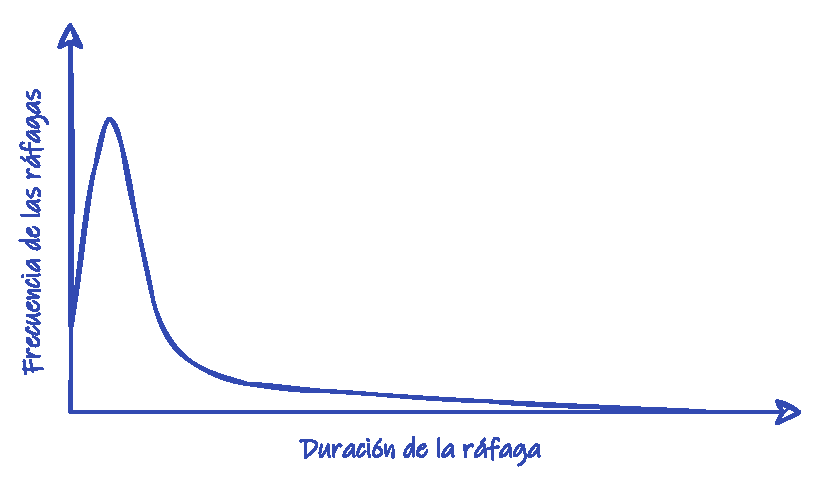
\includegraphics[width=0.8\textwidth]{media/C14_planificación/histogramas_tiempo_de_ráfagas.pdf}
\caption{Histograma de los tiempos de las ráfagas de
CPU.}\label{fig-ruxe1fagas-de-cpu}
\end{figure}

La curva que relaciona la frecuencia de las ráfagas de CPU con la
duración de las mismas tiende a ser exponencial o hiperexponencial
(véase la \hyperref[fig-ruxe1fagas-de-cpu]{Histograma de los tiempos de
las ráfagas de CPU.}) aunque varía enormemente entre tipos de tareas y
sistemas informáticos distintos. Esto significa que los procesos se
pueden clasificar entre aquellos que presentan un gran número de ráfagas
de CPU cortas o aquellos con un pequeño número de ráfagas de CPU largas.

Concretamente:

\begin{itemize}
\item
  Decimos que un proceso es \textbf{limitado por la E/S} cuando presenta
  muchas ráfagas de CPU cortas, debido a que si es así, es porque pasa
  la mayor parte del tiempo esperando por la E/S.
\item
  Decimos que un proceso está \textbf{limitado por la CPU} cuando
  presenta pocas ráfagas de CPU largas, debido a que si es así, es
  porque hace un uso intensivo de la misma y a penas pasa tiempo
  esperando por la E/S.
\end{itemize}

Esta distinción entre tipos de procesos puede ser importante en la
selección de un algoritmo de planificación de CPU adecuado, puesto que,
por lo general el algoritmo escogido debe planificar antes a los
procesos limitados por la E/S, evitando así que los procesos limitados
por la CPU ---que son los que tienden a usarla más tiempo--- la
acaparen.

Si esto último ocurriera, los procesos limitados por la E/S se
acumularían en la \textbf{cola de preparados}, dejando vacías las colas
de dispositivos. Este fenómeno, que provoca una infrautilización de los
dispositivos de E/S, se denomina \textbf{{}efecto convoy}.

Planificar primero a los procesos limitados por la E/S tiene además dos
efectos muy positivos:

\begin{itemize}
\item
  Los procesos interactivos son generalmente procesos limitados por la
  E/S, por lo que planificarlos primero hace que mejore el tiempo de
  respuesta.
\item
  Generalmente el tiempo de espera promedio se reduce cuando se
  planifican primero los procesos con ráfagas de CPU cortas. Según las
  definiciones anteriores, estos procesos son precisamente los limitados
  por la E/S.
\end{itemize}

\section{Algoritmos de planificación de la
CPU}\label{_algoritmos_de_planificaciuxf3n_de_la_cpu}

A continuación ilustraremos algunos de los algoritmos de planificación
de CPU más comunes. Lo haremos considerando que cada proceso tiene una
única ráfaga de CPU. Sin embargo, no debemos olvidar que para ser
precisos necesitaríamos utilizar muchos más procesos, donde cada uno
estuviera compuesto de una secuencia de miles de ráfagas alternativas de
CPU y de E/S.

\subsection{Planificación FCFS}\label{_planificaciuxf3n_fcfs}

{} En la planificación \textbf{{}FCFS} (\emph{First Come, First Served})
o \textbf{primero que llega, primero servido} la cola es FIFO:

\begin{itemize}
\item
  Los procesos que llegan se colocan al final de la cola que les
  corresponde.
\item
  El proceso asignado a la CPU se coge siempre del principio de la cola
  seleccionada.
\item
  Es un algoritmo \textbf{cooperativo}, puesto que un proceso mantiene
  la CPU hasta que decide liberarla voluntariamente ---recordemos que la
  ráfaga de CPU llega a su fin porque el proceso termina o solicita
  alguna operación que lo lleva el estado \textbf{esperando}---.
\end{itemize}

Ilustremos el algoritmo con un ejemplo. Supongamos que 4 procesos llegan
a la \textbf{cola de preparados} en los tiempos indicados en la
\hyperref[tabla-problema-fcfs]{Problema de planificación de la CPU
mediante algoritmo FCFS.}. Además, aunque es difícil tener un
conocimiento a priori del tiempo de la ráfaga de CPU de cada proceso,
vamos a suponer que también son conocidos.

\begin{longtable}[]{@{}
  >{\raggedright\arraybackslash}p{(\linewidth - 4\tabcolsep) * \real{0.3333}}
  >{\raggedright\arraybackslash}p{(\linewidth - 4\tabcolsep) * \real{0.3333}}
  >{\raggedright\arraybackslash}p{(\linewidth - 4\tabcolsep) * \real{0.3333}}@{}}
\caption{Problema de planificación de la CPU mediante algoritmo
FCFS.}\label{tabla-problema-fcfs}\tabularnewline
\toprule\noalign{}
\begin{minipage}[b]{\linewidth}\centering
Proceso
\end{minipage} & \begin{minipage}[b]{\linewidth}\centering
Tiempo de llegada (ms)
\end{minipage} & \begin{minipage}[b]{\linewidth}\centering
Tiempo de ráfaga de CPU (ms)
\end{minipage} \\
\midrule\noalign{}
\endfirsthead
\toprule\noalign{}
\begin{minipage}[b]{\linewidth}\centering
Proceso
\end{minipage} & \begin{minipage}[b]{\linewidth}\centering
Tiempo de llegada (ms)
\end{minipage} & \begin{minipage}[b]{\linewidth}\centering
Tiempo de ráfaga de CPU (ms)
\end{minipage} \\
\midrule\noalign{}
\endhead
\bottomrule\noalign{}
\endlastfoot
P1 & 0 & 24 \\
P2 & 1 & 3 \\
P3 & 2 & 3 \\
P4 & 3 & 2 \\
\end{longtable}

En la siguiente figura podemos ver el
\href{https://es.wikipedia.org/wiki/Diagrama_de_Gantt}{diagrama de
Gantt} de la planificación considerando que se utiliza el algoritmo
\textbf{FCFS}:

\begin{figure}
\centering
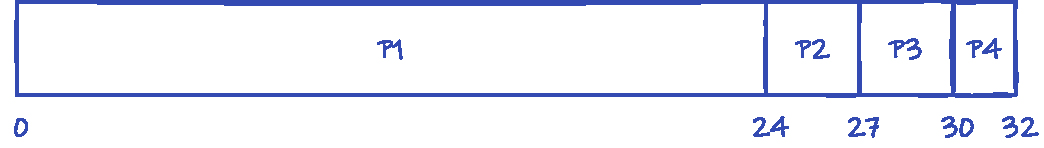
\includegraphics[width=0.8\textwidth]{media/C14_planificación/fcfs1.pdf}
\caption{}
\end{figure}

Utilizando el diagrama anterior, podemos calcular fácilmente los
\textbf{tiempos de espera y de ejecución promedio}:

\begin{longtable}[]{@{}
  >{\raggedright\arraybackslash}p{(\linewidth - 10\tabcolsep) * \real{0.2857}}
  >{\raggedright\arraybackslash}p{(\linewidth - 10\tabcolsep) * \real{0.1429}}
  >{\raggedright\arraybackslash}p{(\linewidth - 10\tabcolsep) * \real{0.1429}}
  >{\raggedright\arraybackslash}p{(\linewidth - 10\tabcolsep) * \real{0.1429}}
  >{\raggedright\arraybackslash}p{(\linewidth - 10\tabcolsep) * \real{0.1429}}
  >{\raggedright\arraybackslash}p{(\linewidth - 10\tabcolsep) * \real{0.1429}}@{}}
\toprule\noalign{}
\begin{minipage}[b]{\linewidth}\centering
Proceso
\end{minipage} & \begin{minipage}[b]{\linewidth}\centering
Instante de finalización (ms)
\end{minipage} &
\multicolumn{2}{>{\centering\arraybackslash}p{(\linewidth - 10\tabcolsep) * \real{0.2857} + 2\tabcolsep}}{\begin{minipage}[b]{\linewidth}\centering
Tiempo de espera (ms)
\end{minipage} &
\multicolumn{2}{>{\centering\arraybackslash}p{(\linewidth - 10\tabcolsep) * \real{0.2857} + 2\tabcolsep}@{}}{\begin{minipage}[b]{\linewidth}\centering
Tiempo de ejecución (ms)
\end{minipage} \\
\midrule\noalign{}
\endhead
\bottomrule\noalign{}
\endlastfoot
P1 & 24 & {(0-0)=} & 0 & {(24-0)=} & 24 \\
P2 & 27 & {(24-1)=} & 23 & {(27-1)=} & 26 \\
P3 & 30 & {(27-2)=} & 25 & {(30-2)=} & 28 \\
P4 & 32 & {(30-3)=} & 27 & {(32-3)=} & 29 \\
\end{longtable}

Lo interesante es que el resultado cambia si los procesos llegan en otro
orden. Por ejemplo, P1 podría llegar el último:

\begin{longtable}[]{@{}
  >{\raggedright\arraybackslash}p{(\linewidth - 4\tabcolsep) * \real{0.3333}}
  >{\raggedright\arraybackslash}p{(\linewidth - 4\tabcolsep) * \real{0.3333}}
  >{\raggedright\arraybackslash}p{(\linewidth - 4\tabcolsep) * \real{0.3333}}@{}}
\toprule\noalign{}
\begin{minipage}[b]{\linewidth}\centering
Proceso
\end{minipage} & \begin{minipage}[b]{\linewidth}\centering
Tiempo de llegada (ms)
\end{minipage} & \begin{minipage}[b]{\linewidth}\centering
Tiempo de ráfaga de CPU (ms)
\end{minipage} \\
\midrule\noalign{}
\endhead
\bottomrule\noalign{}
\endlastfoot
P2 & 0 & 3 \\
P3 & 1 & 3 \\
P4 & 2 & 2 \\
P1 & 3 & 24 \\
\end{longtable}

Entonces el resultado de la planificación sería el que se muestra en la
siguiente figura:

\begin{figure}
\centering
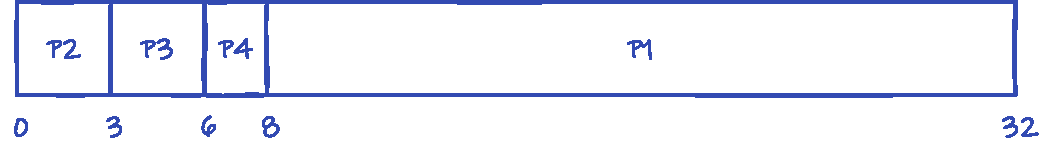
\includegraphics[width=0.8\textwidth]{media/C14_planificación/fcfs2.pdf}
\caption{}
\end{figure}

Y los \textbf{tiempos de espera y ejecución promedio} correspondientes
serían:

\begin{longtable}[]{@{}
  >{\raggedright\arraybackslash}p{(\linewidth - 10\tabcolsep) * \real{0.2857}}
  >{\raggedright\arraybackslash}p{(\linewidth - 10\tabcolsep) * \real{0.1429}}
  >{\raggedright\arraybackslash}p{(\linewidth - 10\tabcolsep) * \real{0.1429}}
  >{\raggedright\arraybackslash}p{(\linewidth - 10\tabcolsep) * \real{0.1429}}
  >{\raggedright\arraybackslash}p{(\linewidth - 10\tabcolsep) * \real{0.1429}}
  >{\raggedright\arraybackslash}p{(\linewidth - 10\tabcolsep) * \real{0.1429}}@{}}
\toprule\noalign{}
\begin{minipage}[b]{\linewidth}\centering
Proceso
\end{minipage} & \begin{minipage}[b]{\linewidth}\centering
Instante de finalización (ms)
\end{minipage} &
\multicolumn{2}{>{\centering\arraybackslash}p{(\linewidth - 10\tabcolsep) * \real{0.2857} + 2\tabcolsep}}{\begin{minipage}[b]{\linewidth}\centering
Tiempo de espera (ms)
\end{minipage} &
\multicolumn{2}{>{\centering\arraybackslash}p{(\linewidth - 10\tabcolsep) * \real{0.2857} + 2\tabcolsep}@{}}{\begin{minipage}[b]{\linewidth}\centering
Tiempo de ejecución (ms)
\end{minipage} \\
\midrule\noalign{}
\endhead
\bottomrule\noalign{}
\endlastfoot
P2 & 3 & {(0-0)=} & 0 & {(3-0)=} & 3 \\
P3 & 6 & {(3-1)=} & 2 & {(6-1)=} & 5 \\
P4 & 8 & {(6-2)=} & 4 & {(8-2)=} & 6 \\
P1 & 32 & {(8-3)=} & 5 & {(32-3)=} & 29 \\
\end{longtable}

Aunque el tiempo total necesario para ejecutar las ráfagas de los 4
procesos, los criterios utilizados reflejan que el algoritmo se comporta
mucho mejor en el segundo caso. Por tanto, el algoritmo \textbf{FCFS} no
garantiza ni \textbf{tiempos de espera} ni de \textbf{ejecución}
mínimos, ya que pueden cambiar variar considerablemente con el orden en
el que llegan los procesos.

Además, el algoritmo \textbf{FCFS} sufre el llamado \textbf{{}efecto
convoy}. Para entenderlo, analicemos lo que está pasando en el ejemplo
de la \hyperref[tabla-problema-fcfs]{Problema de planificación de la CPU
mediante algoritmo FCFS.}:

\begin{enumerate}
\def\labelenumi{\arabic{enumi}.}
\item
  Al proceso P1 se le asigna la CPU. Durante el tiempo que P1 utiliza la
  CPU todos los otros procesos terminan sus operaciones de E/S y pasan a
  la \textbf{cola de preparados}. Por tanto, mientras los procesos
  esperan para utilizar la CPU, los dispositivos de E/S permanecen
  desocupados.
\item
  El proceso P1 termina de usar la CPU y pasa a una cola de
  dispositivos.
\item
  El resto de procesos P, que tienen ráfagas de CPU cortas, se ejecutan
  rápidamente y pasan a las colas de dispositivos. Por tanto, la CPU
  permanecerá vacía hasta que algún proceso termine la operación de E/S
  solicitada.
\item
  El proceso P1 pasa a la \textbf{cola de preparados} y se le asigna la
  CPU. Con el tiempo el resto de procesos terminarán sus operaciones y,
  nuevamente, tienen que esperar en la \textbf{cola de preparados} a que
  el proceso P1 termine de utilizarla.
\end{enumerate}

Esto nos permite llegar a la conclusión de que en cierto orden de
llegada la mayor parte de los procesos esperan constantemente detrás de
uno para poder realizar su trabajo. Esto reduce la utilización de la CPU
y de los dispositivos de E/S por debajo de lo que sería posible, si los
procesos más cortos se ejecutasen primero.

\subsection{Planificación SJF}\label{_planificaciuxf3n_sjf}

{} La planificación \textbf{{}SJF} (\emph{Shortest-Job First}) o
\textbf{primero el más corto}, consiste en:

\begin{enumerate}
\def\labelenumi{\arabic{enumi}.}
\item
  Se asocia con cada proceso la longitud de tiempo de su siguiente
  ráfaga de CPU.
\item
  Cuando la CPU está disponible, se pone \textbf{ejecutando} el proceso
  de menor ráfaga de CPU.
\item
  Si dos procesos tienen ráfagas de una misma longitud, se utiliza el
  algoritmo \textbf{FCFS} ---entre ellos, el que lleva más tiempo en la
  \textbf{cola de preparados}---.
\item
  Es un algoritmo \textbf{cooperativo}, puesto que un proceso mantiene
  la CPU hasta que decide liberarla voluntariamente.
\end{enumerate}

Ilustremos el algoritmo con un ejemplo:

\begin{longtable}[]{@{}
  >{\raggedright\arraybackslash}p{(\linewidth - 4\tabcolsep) * \real{0.3333}}
  >{\raggedright\arraybackslash}p{(\linewidth - 4\tabcolsep) * \real{0.3333}}
  >{\raggedright\arraybackslash}p{(\linewidth - 4\tabcolsep) * \real{0.3333}}@{}}
\toprule\noalign{}
\begin{minipage}[b]{\linewidth}\centering
Proceso
\end{minipage} & \begin{minipage}[b]{\linewidth}\centering
Tiempo de llegada (ms)
\end{minipage} & \begin{minipage}[b]{\linewidth}\centering
Tiempo de ráfaga de CPU (ms)
\end{minipage} \\
\midrule\noalign{}
\endhead
\bottomrule\noalign{}
\endlastfoot
P1 & 0 & 6 \\
P2 & 1 & 8 \\
P3 & 2 & 7 \\
P4 & 3 & 3 \\
\end{longtable}

Considerando que se utiliza el algoritmo \textbf{SJF} obtendremos el
siguiente diagrama de Gantt:

\begin{figure}
\centering
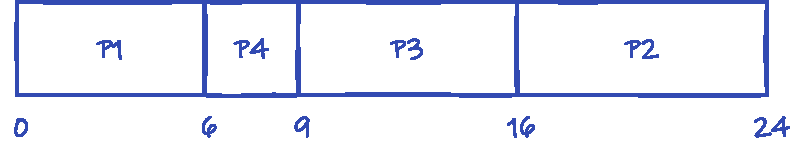
\includegraphics[width=0.8\textwidth]{media/C14_planificación/sjf.pdf}
\caption{}
\end{figure}

Con los \textbf{tiempos de espera y ejecución promedio}
correspondientes:

\begin{longtable}[]{@{}
  >{\raggedright\arraybackslash}p{(\linewidth - 10\tabcolsep) * \real{0.2857}}
  >{\raggedright\arraybackslash}p{(\linewidth - 10\tabcolsep) * \real{0.1429}}
  >{\raggedright\arraybackslash}p{(\linewidth - 10\tabcolsep) * \real{0.1429}}
  >{\raggedright\arraybackslash}p{(\linewidth - 10\tabcolsep) * \real{0.1429}}
  >{\raggedright\arraybackslash}p{(\linewidth - 10\tabcolsep) * \real{0.1429}}
  >{\raggedright\arraybackslash}p{(\linewidth - 10\tabcolsep) * \real{0.1429}}@{}}
\toprule\noalign{}
\begin{minipage}[b]{\linewidth}\centering
Proceso
\end{minipage} & \begin{minipage}[b]{\linewidth}\centering
Instante de finalización (ms)
\end{minipage} &
\multicolumn{2}{>{\centering\arraybackslash}p{(\linewidth - 10\tabcolsep) * \real{0.2857} + 2\tabcolsep}}{\begin{minipage}[b]{\linewidth}\centering
Tiempo de espera (ms)
\end{minipage} &
\multicolumn{2}{>{\centering\arraybackslash}p{(\linewidth - 10\tabcolsep) * \real{0.2857} + 2\tabcolsep}@{}}{\begin{minipage}[b]{\linewidth}\centering
Tiempo de ejecución (ms)
\end{minipage} \\
\midrule\noalign{}
\endhead
\bottomrule\noalign{}
\endlastfoot
P1 & 6 & {(0-0)=} & 0 & {(6-0)=} & 6 \\
P2 & 24 & {(16-1)=} & 15 & {(24-1)=} & 23 \\
P3 & 16 & {(9-2)=} & 7 & {(16-2)=} & 14 \\
P4 & 9 & {(6-3)=} & 3 & {(9-3)=} & 6 \\
\end{longtable}

Sin embargo, si hubiéramos utilizado el algoritmo \textbf{FCFS}:

\begin{figure}
\centering
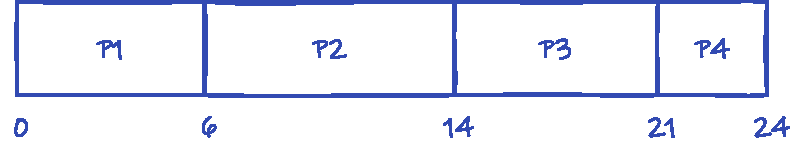
\includegraphics[width=0.8\textwidth]{media/C14_planificación/fcfs-sjf.pdf}
\caption{}
\end{figure}

\begin{longtable}[]{@{}
  >{\raggedright\arraybackslash}p{(\linewidth - 10\tabcolsep) * \real{0.2857}}
  >{\raggedright\arraybackslash}p{(\linewidth - 10\tabcolsep) * \real{0.1429}}
  >{\raggedright\arraybackslash}p{(\linewidth - 10\tabcolsep) * \real{0.1429}}
  >{\raggedright\arraybackslash}p{(\linewidth - 10\tabcolsep) * \real{0.1429}}
  >{\raggedright\arraybackslash}p{(\linewidth - 10\tabcolsep) * \real{0.1429}}
  >{\raggedright\arraybackslash}p{(\linewidth - 10\tabcolsep) * \real{0.1429}}@{}}
\toprule\noalign{}
\begin{minipage}[b]{\linewidth}\centering
Proceso
\end{minipage} & \begin{minipage}[b]{\linewidth}\centering
Instante de finalización (ms)
\end{minipage} &
\multicolumn{2}{>{\centering\arraybackslash}p{(\linewidth - 10\tabcolsep) * \real{0.2857} + 2\tabcolsep}}{\begin{minipage}[b]{\linewidth}\centering
Tiempo de espera (ms)
\end{minipage} &
\multicolumn{2}{>{\centering\arraybackslash}p{(\linewidth - 10\tabcolsep) * \real{0.2857} + 2\tabcolsep}@{}}{\begin{minipage}[b]{\linewidth}\centering
Tiempo de ejecución (ms)
\end{minipage} \\
\midrule\noalign{}
\endhead
\bottomrule\noalign{}
\endlastfoot
P1 & 6 & {(0-0)=} & 0 & {(6-0)=} & 6 \\
P2 & 14 & {(6-1)=} & 5 & {(14-1)=} & 13 \\
P3 & 21 & {(14-2)=} & 12 & {(21-2)=} & 19 \\
P4 & 24 & {(21-3)=} & 18 & {(24-3)=} & 21 \\
\end{longtable}

El algoritmo \textbf{SJF} es óptimo en el sentido de que el
\textbf{tiempo de espera promedio} es mínimo, porque reduce más el
tiempo de espera de los procesos cortos y aumenta el de los procesos
largos. Además, así se evita el \textbf{efecto convoy}.

Sin embargo, la pregunta que debemos hacernos es cómo podemos conocer de
antemano la longitud de las ráfagas de CPU de un proceso, para usar esa
información durante la planificación. Sin analizar el código, el sistema
operativo no puede conocer el tiempo de una ráfaga hasta que esta no
termina de ejecutarse.

Por eso el algoritmo SJF se utiliza frecuentemente como planificador de
la \textbf{cola de trabajos}, donde se puede obligar al usuario a
especificar un tiempo de ejecución máximo, al enviar el trabajo a dicha
cola. En este caso, los usuarios tenderán a ajustar la estimación de
tiempo de ejecución, puesto que los que tengan tiempos más cortos serán
priorizados para ser ejecutados antes, frente a los de tiempos más
largos.

Para evitar que los usuarios hagan trampas indicando un tiempo de
ejecución más corto que el real, con el fin de que se planifique antes
su trabajo, se puede utilizar un temporizador para abortar los trabajos
que excedan el tiempo de ejecución indicado por el usuario. El error
puede ser notificado al usuario para que vuelva a enviar el trabajo con
una estimación más realista.

Para utilizar el algoritmo \textbf{SJF} en el planificador de la CPU, lo
único que se puede hacer es intentar predecir el tiempo de la siguiente
ráfaga de CPU. Por ejemplo, se puede utilizar un promedio ponderado
exponencial de los tiempos de las de ráfagas de CPU pasadas:

\[tau_(n+1) = alpha*t_n + (1 - alpha)*tau_n, 0 le alpha le 1\]

donde:

\begin{itemize}
\item
  \(tau_(n+1)\) es la estimación de tiempo de la siguiente ráfaga de CPU
\item
  \(t_n\) es el tiempo real de la última ráfaga
\item
  \(alpha\) es el peso relativo del tiempo real de la última ráfaga.
\item
  \(tau_(n)\) es la estimación de tiempo de la última ráfaga.
\end{itemize}

La expresión es recursiva, dado que \(tau_n\) se calcula usando la
ecuación con \(t_(n-1)\) y \(tau_(n-1)\); que a su vez depende de
\(t_(n-2)\) y \(tau_(n-2)\), y así sucesivamente.

Si desarrollamos la fórmula sustituyendo los valores, veremos que
\(t_n\) se pondera con \(alpha\), \(t_(n-1)\) con \((1 - alpha)alpha\),
\(t_(n-2)\) con \((1 - alpha)^2alpha\), y así sucesivamente:

\[tau_(n+1) = alpha*t_n + (1 - alpha)*alpha*t_(n-1) + (1 - alpha)^2*alpha*t_(n-2) + ...\]

Si \(alpha\) = 1, \(tau_(n+1)\) = \(alpha*t_n\), ignorando el resto del
histórico. En otro caso, dado que tanto \(alpha\) como \(1 - alpha\) son
menores de 1, cada término sucesivo tiene menor peso que su predecesor,
haciendo que los \(t_n\) contribuyan menos cuanto más alejados del
tiempo actual.

El problema es que todos estos cálculos consumen tiempo de CPU, cuando
el planificador debe ser lo más rápido posible, dado que se ejecuta con
mucha frecuencia.

\subsection{Planificación SRTF}\label{_planificaciuxf3n_srtf}

{} El algoritmo \textbf{SJF} es \textbf{cooperativo}, pero se puede
implementar de forma \textbf{expropiativa}, en cuyo caso se llama
\textbf{{}SRTF} (Shortest-Remaing-Time First). La diferencia está en lo
que ocurre cuando un nuevo proceso llega a la \textbf{cola de
preparados}.

En \textbf{SRTF} se compara el tiempo de la siguiente ráfaga de CPU del
nuevo proceso, con el tiempo de ráfaga que le queda al proceso en
ejecución. Si la primera magnitud es inferior, el proceso que tiene la
CPU es expropiado y sustituido por el nuevo proceso. Mientras que en
\textbf{SJF} no se hace nada. Se espera que el proceso que actualmente
se está ejecutando termine su ráfaga de CPU voluntariamente.

Ilustremos el algoritmo con un ejemplo:

\begin{longtable}[]{@{}
  >{\raggedright\arraybackslash}p{(\linewidth - 4\tabcolsep) * \real{0.3333}}
  >{\raggedright\arraybackslash}p{(\linewidth - 4\tabcolsep) * \real{0.3333}}
  >{\raggedright\arraybackslash}p{(\linewidth - 4\tabcolsep) * \real{0.3333}}@{}}
\toprule\noalign{}
\begin{minipage}[b]{\linewidth}\centering
Proceso
\end{minipage} & \begin{minipage}[b]{\linewidth}\centering
Tiempo de llegada (ms)
\end{minipage} & \begin{minipage}[b]{\linewidth}\centering
Tiempo de ráfaga de CPU (ms)
\end{minipage} \\
\midrule\noalign{}
\endhead
\bottomrule\noalign{}
\endlastfoot
P1 & 0 & 8 \\
P2 & 1 & 4 \\
P3 & 2 & 9 \\
P4 & 3 & 5 \\
\end{longtable}

El resultado es el que se muestra en el siguiente diagrama de Gantt:

\begin{figure}
\centering
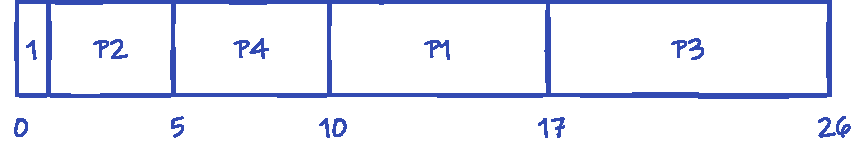
\includegraphics[width=0.8\textwidth]{media/C14_planificación/srtf.pdf}
\caption{}
\end{figure}

Y los tiempos de espera y ejecución promedio correspondientes serían:

\begin{longtable}[]{@{}
  >{\raggedright\arraybackslash}p{(\linewidth - 10\tabcolsep) * \real{0.2857}}
  >{\raggedright\arraybackslash}p{(\linewidth - 10\tabcolsep) * \real{0.1429}}
  >{\raggedright\arraybackslash}p{(\linewidth - 10\tabcolsep) * \real{0.1429}}
  >{\raggedright\arraybackslash}p{(\linewidth - 10\tabcolsep) * \real{0.1429}}
  >{\raggedright\arraybackslash}p{(\linewidth - 10\tabcolsep) * \real{0.1429}}
  >{\raggedright\arraybackslash}p{(\linewidth - 10\tabcolsep) * \real{0.1429}}@{}}
\toprule\noalign{}
\begin{minipage}[b]{\linewidth}\centering
Proceso
\end{minipage} & \begin{minipage}[b]{\linewidth}\centering
Instante de finalización (ms)
\end{minipage} &
\multicolumn{2}{>{\centering\arraybackslash}p{(\linewidth - 10\tabcolsep) * \real{0.2857} + 2\tabcolsep}}{\begin{minipage}[b]{\linewidth}\centering
Tiempo de espera (ms)
\end{minipage} &
\multicolumn{2}{>{\centering\arraybackslash}p{(\linewidth - 10\tabcolsep) * \real{0.2857} + 2\tabcolsep}@{}}{\begin{minipage}[b]{\linewidth}\centering
Tiempo de ejecución (ms)
\end{minipage} \\
\midrule\noalign{}
\endhead
\bottomrule\noalign{}
\endlastfoot
P1 & 17 & {(0-0) + (10-1)=} & 9 & {(17-0)=} & 17 \\
P2 & 5 & {(1-1)=} & 0 & {(5-1)=} & 4 \\
P3 & 26 & {(17-2)=} & 15 & {(26-2)=} & 24 \\
P4 & 10 & {(5-3)=} & 2 & {(10-3)=} & 7 \\
\end{longtable}

Es muy complicado predecir cuál de los dos algoritmos será mejor para un
conjunto concreto de procesos. Sin embargo, debemos tener en cuenta que
---aunque no lo estemos considerando en estos problemas--- un algoritmo
expropitativo, por lo general, provocará más cambios de contexto en los
que se perderá tiempo de CPU.

Los algoritmos expropiativos también suelen ofrecer mejores tiempos de
respuesta, puesto que un proceso que llega a la \textbf{cola de
preparados} puede ser asignado a la CPU sin esperar a que el proceso que
se ejecuta en ella actualmente termine su ráfaga de CPU.

\subsection{Planificación con
prioridades}\label{_planificaciuxf3n_con_prioridades}

{} En la \textbf{planificación con prioridades} se asocia una prioridad
a cada proceso, de tal forma que el de prioridad más alta es asignado a
la CPU. En caso de igual prioridad, se utiliza \textbf{FCFS}.

Las prioridades se suelen indicar con números enteros en un rango fijo.
Por ejemplo {[}0-7{]}, {[}0-31{]}, {[}0-139{]} o {[}0-4095{]}. En
algunos sistemas operativos los números más grandes representan mayor
prioridad, mientras que en otros son los procesos con números más
pequeños los que se planifican primero. En este curso utilizaremos la
convención de que a menor valor, mayor prioridad.

Si las prioridades se asignan en relación con el tiempo de la próxima
ráfaga de CPU, su comportamiento es el mismo que el del \textbf{SJF};
por lo que se considera a este último un caso particular de algoritmo de
\textbf{planificación con prioridades}.

El algoritmo de planificación con prioridades puede ser
\textbf{expropiativo} o \textbf{cooperativo}:

\begin{itemize}
\item
  En el caso \textbf{expropiativo}, cuando un proceso llega a la
  \textbf{cola de preparados} su prioridad es comparada con la del
  proceso en ejecución. Se expropia la CPU si la prioridad del nuevo
  proceso es superior a la prioridad del proceso que se ejecuta.
\item
  En el caso \textbf{cooperativo}, no se toma ninguna decisión cuando
  llega un proceso a la \textbf{cola de preparados}, solo cuando el que
  tiene asignada la CPU la abandona.
\end{itemize}

Supongamos que 5 procesos llegan a la cola de preparados en los tiempos
indicados en la \hyperref[tabla-problema-prioridad]{Problema de
planificación de la CPU mediante algoritmo de planificación con
prioridades.}. Como en los ejemplos anteriores, aunque es difícil tener
un conocimiento a priori del tiempo de las ráfagas de CPU, vamos a
suponer que son conocidos. Y también que a cada proceso se le asigna, de
alguna forma, una prioridad cuando llega a la \textbf{cola de
preparados}.

\begin{longtable}[]{@{}
  >{\raggedright\arraybackslash}p{(\linewidth - 6\tabcolsep) * \real{0.2500}}
  >{\raggedright\arraybackslash}p{(\linewidth - 6\tabcolsep) * \real{0.2500}}
  >{\raggedright\arraybackslash}p{(\linewidth - 6\tabcolsep) * \real{0.2500}}
  >{\raggedright\arraybackslash}p{(\linewidth - 6\tabcolsep) * \real{0.2500}}@{}}
\caption{Problema de planificación de la CPU mediante algoritmo de
planificación con
prioridades.}\label{tabla-problema-prioridad}\tabularnewline
\toprule\noalign{}
\begin{minipage}[b]{\linewidth}\centering
Proceso
\end{minipage} & \begin{minipage}[b]{\linewidth}\centering
Tiempo de llegada (ms)
\end{minipage} & \begin{minipage}[b]{\linewidth}\centering
Tiempo de ráfaga de CPU (ms)
\end{minipage} & \begin{minipage}[b]{\linewidth}\centering
Prioridad
\end{minipage} \\
\midrule\noalign{}
\endfirsthead
\toprule\noalign{}
\begin{minipage}[b]{\linewidth}\centering
Proceso
\end{minipage} & \begin{minipage}[b]{\linewidth}\centering
Tiempo de llegada (ms)
\end{minipage} & \begin{minipage}[b]{\linewidth}\centering
Tiempo de ráfaga de CPU (ms)
\end{minipage} & \begin{minipage}[b]{\linewidth}\centering
Prioridad
\end{minipage} \\
\midrule\noalign{}
\endhead
\bottomrule\noalign{}
\endlastfoot
P1 & 0 & 10 & 3 \\
P2 & 1 & 2 & 1 \\
P3 & 2 & 3 & 4 \\
P4 & 3 & 2 & 5 \\
P5 & 4 & 5 & 2 \\
\end{longtable}

En las condiciones anteriores, si utilizamos el algoritmo de
planificación por prioridades expropiativo, obtendremos el diagrama de
Gantt de la siguiente figura:

\begin{figure}
\centering
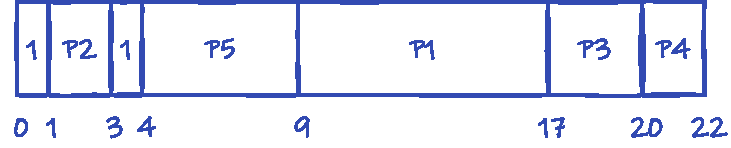
\includegraphics[width=0.8\textwidth]{media/C14_planificación/prioridad.pdf}
\caption{}
\end{figure}

Con los \textbf{tiempos de espera y ejecución promedio}
correspondientes:

\begin{longtable}[]{@{}
  >{\raggedright\arraybackslash}p{(\linewidth - 10\tabcolsep) * \real{0.2857}}
  >{\raggedright\arraybackslash}p{(\linewidth - 10\tabcolsep) * \real{0.1429}}
  >{\raggedright\arraybackslash}p{(\linewidth - 10\tabcolsep) * \real{0.1429}}
  >{\raggedright\arraybackslash}p{(\linewidth - 10\tabcolsep) * \real{0.1429}}
  >{\raggedright\arraybackslash}p{(\linewidth - 10\tabcolsep) * \real{0.1429}}
  >{\raggedright\arraybackslash}p{(\linewidth - 10\tabcolsep) * \real{0.1429}}@{}}
\toprule\noalign{}
\begin{minipage}[b]{\linewidth}\centering
Proceso
\end{minipage} & \begin{minipage}[b]{\linewidth}\centering
Instante de finalización (ms)
\end{minipage} &
\multicolumn{2}{>{\centering\arraybackslash}p{(\linewidth - 10\tabcolsep) * \real{0.2857} + 2\tabcolsep}}{\begin{minipage}[b]{\linewidth}\centering
Tiempo de espera (ms)
\end{minipage} &
\multicolumn{2}{>{\centering\arraybackslash}p{(\linewidth - 10\tabcolsep) * \real{0.2857} + 2\tabcolsep}@{}}{\begin{minipage}[b]{\linewidth}\centering
Tiempo de ejecución (ms)
\end{minipage} \\
\midrule\noalign{}
\endhead
\bottomrule\noalign{}
\endlastfoot
P1 & 4 & {(0-0) + (3-1) + (9-4)=} & 7 & {(17-0)=} & 17 \\
P2 & 3 & {(1-1)=} & 0 & {(3-1)=} & 2 \\
P3 & 20 & {(17-2)=} & 15 & {(20-2)=} & 18 \\
P4 & 22 & {(20-3)=} & 17 & {(22-3)=} & 19 \\
P5 & 9 & {(4-4)=} & 0 & {(9-4)=} & 5 \\
\end{longtable}

Mientras que si utilizamos el algoritmo de planificación por prioridades
cooperativo, obtendremos el diagrama de Gantt de la siguiente figura:

\begin{figure}
\centering
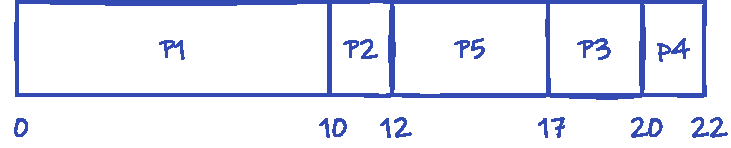
\includegraphics[width=0.8\textwidth]{media/C14_planificación/prioridad_cooperativo.pdf}
\caption{}
\end{figure}

Con los \textbf{tiempos de espera y ejecución promedio}
correspondientes:

\begin{longtable}[]{@{}
  >{\raggedright\arraybackslash}p{(\linewidth - 10\tabcolsep) * \real{0.2857}}
  >{\raggedright\arraybackslash}p{(\linewidth - 10\tabcolsep) * \real{0.1429}}
  >{\raggedright\arraybackslash}p{(\linewidth - 10\tabcolsep) * \real{0.1429}}
  >{\raggedright\arraybackslash}p{(\linewidth - 10\tabcolsep) * \real{0.1429}}
  >{\raggedright\arraybackslash}p{(\linewidth - 10\tabcolsep) * \real{0.1429}}
  >{\raggedright\arraybackslash}p{(\linewidth - 10\tabcolsep) * \real{0.1429}}@{}}
\toprule\noalign{}
\begin{minipage}[b]{\linewidth}\centering
Proceso
\end{minipage} & \begin{minipage}[b]{\linewidth}\centering
Instante de finalización (ms)
\end{minipage} &
\multicolumn{2}{>{\centering\arraybackslash}p{(\linewidth - 10\tabcolsep) * \real{0.2857} + 2\tabcolsep}}{\begin{minipage}[b]{\linewidth}\centering
Tiempo de espera (ms)
\end{minipage} &
\multicolumn{2}{>{\centering\arraybackslash}p{(\linewidth - 10\tabcolsep) * \real{0.2857} + 2\tabcolsep}@{}}{\begin{minipage}[b]{\linewidth}\centering
Tiempo de ejecución (ms)
\end{minipage} \\
\midrule\noalign{}
\endhead
\bottomrule\noalign{}
\endlastfoot
P1 & 10 & {(0-0)=} & 0 & {(10-0)=} & 10 \\
P2 & 12 & {(10-1)=} & 9 & {(12-1)=} & 11 \\
P3 & 20 & {(17-2)=} & 15 & {(20-2)=} & 18 \\
P4 & 22 & {(20-3)=} & 17 & {(22-3)=} & 19 \\
P5 & 17 & {(12-4)=} & 8 & {(17-4)=} & 13 \\
\end{longtable}

Que estos algoritmos ofrezcan mejores o peores resultados que otros,
obviamente depende de los criterios utilizados para asignar las
prioridades.

\subsubsection{Prioridades definidas internamente o
externamente}\label{_prioridades_definidas_internamente_o_externamente}

Hay dos maneras de asignar las prioridades:

\begin{itemize}
\item
  \textbf{Internamente}. Se utiliza una cualidad medible del proceso
  para calcular su prioridad. Por ejemplo, límites de tiempo,
  necesidades de memoria, número de archivos abiertos, tiempo estimado
  de ráfaga de CPU ---como en \textbf{SJF}--- o la proporción entre esta
  y el tiempo estimado de ráfaga de E/S.
\item
  \textbf{Externamente}. Las prioridades son fijadas por criterios
  externos al sistema operativo. Por ejemplo, la importancia del proceso
  para los usuarios, la cantidad de dinero pagada para el uso del
  sistema u otros factores políticos.
\end{itemize}

Algunas de estas formas de asignar las prioridades pueden ser fijas,
mientras que otras pueden ser variables. Es decir, un criterio externo
como es la importancia del proceso para los usuarios, puede dar lugar a
una prioridad que se asigna al crear el proceso y que no cambia durante
toda su ejecución. Por el contrario, un criterio como el tiempo de
ráfaga de CPU puede dar lugar a una prioridad variable, que se ajusta
cada vez que se tiene una estimación mejor.

\subsubsection{Muerte por inanición}\label{_muerte_por_inaniciuxf3n}

El mayor problema de este tipo de planificación es el \textbf{bloqueo
indefinido}{} o \textbf{{}muerte por inanición}. Si hay un conjunto de
procesos de alta prioridad demandando CPU continuamente, el algoritmo
puede dejar a algunos procesos de menor prioridad esperando
indefinidamente.

Una solución a este problema es aplicar mecanismos de
\textbf{{}envejecimiento}. Consisten en aumentar gradualmente la
prioridad de los procesos que esperan ---por ejemplo, 1 unidad cada 15
minutos---. De esta manera los proceso de baja prioridad tarde o
temprano tendrán una oportunidad para ejecutarse. Una vez se les asigna
la CPU, se restablece su prioridad al valor original.

\subsection{Planificación RR}\label{_planificaciuxf3n_rr}

{} {} El algoritmo \textbf{{}RR} (\emph{Round-Robin}) es similar al
\textbf{FCFS}, pero añadiendo la expropiación para conmutar entre
procesos cuando llevan cierta cantidad de tiempo ejecutándose en la CPU.

Este algoritmo requiere los siguientes elementos:

\begin{itemize}
\item
  Definir una \textbf{{}ventana de tiempo} o \textbf{{}cuanto},
  generalmente entre 10 y 100 ms
\item
  Definir la \textbf{cola de preparados} como una cola circular, donde
  el planificador asigna la CPU a cada proceso en intervalos de tiempo
  de hasta un \textbf{cuanto}, como máximo.
\end{itemize}

Cuando un proceso está en la CPU pueden darse diversos casos:

\begin{itemize}
\item
  Que la ráfaga de CPU sea menor que un cuanto. Entonces el proceso
  liberará la CPU voluntariamente, al terminar la ráfaga.
\item
  Que la ráfaga de CPU sea mayor que un cuanto. El temporizador
  interrumpirá el proceso al terminar el cuanto e informará al sistema
  operativo. Este hará el cambio de contexto para asignar la CPU al
  siguiente proceso y el que abandona la CPU es insertado al final de la
  \textbf{cola de preparados}.
\end{itemize}

Este algoritmo es \textbf{expropiativo}, puesto que los procesos son
expropiados por la interrupción del temporizador. Como se puede intuir,
originalmente fue diseñado para los \textbf{sistemas de tiempo
compartido}, para repartir la CPU por igual entre los procesos de los
usuarios del sistema.

Ilustremos el algoritmo con un ejemplo con cuanto de 4 ms:

\begin{longtable}[]{@{}
  >{\raggedright\arraybackslash}p{(\linewidth - 4\tabcolsep) * \real{0.3333}}
  >{\raggedright\arraybackslash}p{(\linewidth - 4\tabcolsep) * \real{0.3333}}
  >{\raggedright\arraybackslash}p{(\linewidth - 4\tabcolsep) * \real{0.3333}}@{}}
\toprule\noalign{}
\begin{minipage}[b]{\linewidth}\centering
Proceso
\end{minipage} & \begin{minipage}[b]{\linewidth}\centering
Tiempo de llegada (ms)
\end{minipage} & \begin{minipage}[b]{\linewidth}\centering
Tiempo de ráfaga de CPU (ms)
\end{minipage} \\
\midrule\noalign{}
\endhead
\bottomrule\noalign{}
\endlastfoot
P1 & 0 & 24 \\
P2 & 1 & 3 \\
P3 & 2 & 3 \\
\end{longtable}

El resultado es el que se muestra en el siguiente diagrama de Gantt:

\begin{figure}
\centering
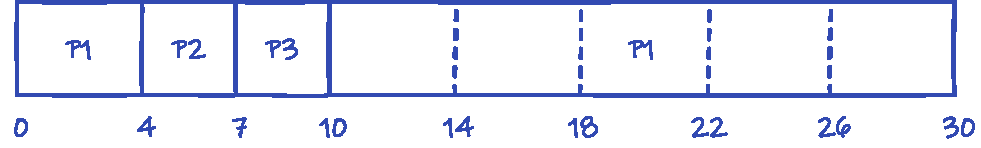
\includegraphics[width=0.8\textwidth]{media/C14_planificación/rr.pdf}
\caption{}
\end{figure}

Y los \textbf{tiempos de espera y ejecución promedio} correspondientes
serían:

\begin{longtable}[]{@{}
  >{\raggedright\arraybackslash}p{(\linewidth - 10\tabcolsep) * \real{0.2857}}
  >{\raggedright\arraybackslash}p{(\linewidth - 10\tabcolsep) * \real{0.1429}}
  >{\raggedright\arraybackslash}p{(\linewidth - 10\tabcolsep) * \real{0.1429}}
  >{\raggedright\arraybackslash}p{(\linewidth - 10\tabcolsep) * \real{0.1429}}
  >{\raggedright\arraybackslash}p{(\linewidth - 10\tabcolsep) * \real{0.1429}}
  >{\raggedright\arraybackslash}p{(\linewidth - 10\tabcolsep) * \real{0.1429}}@{}}
\toprule\noalign{}
\begin{minipage}[b]{\linewidth}\centering
Proceso
\end{minipage} & \begin{minipage}[b]{\linewidth}\centering
Instante de finalización (ms)
\end{minipage} &
\multicolumn{2}{>{\centering\arraybackslash}p{(\linewidth - 10\tabcolsep) * \real{0.2857} + 2\tabcolsep}}{\begin{minipage}[b]{\linewidth}\centering
Tiempo de espera (ms)
\end{minipage} &
\multicolumn{2}{>{\centering\arraybackslash}p{(\linewidth - 10\tabcolsep) * \real{0.2857} + 2\tabcolsep}@{}}{\begin{minipage}[b]{\linewidth}\centering
Tiempo de ejecución (ms)
\end{minipage} \\
\midrule\noalign{}
\endhead
\bottomrule\noalign{}
\endlastfoot
P1 & 30 & {(0-0) + (10-4)=} & 6 & {(30-0)=} & 24 \\
P2 & 7 & {(4-1)=} & 3 & {(7-1)=} & 6 \\
P3 & 10 & {(7-2)=} & 5 & {(10-2)=} & 8 \\
\end{longtable}

\subsubsection{Rendimiento}\label{_rendimiento}

Cuando se utiliza la planificación \textbf{RR} el tamaño del cuanto es
un factor clave en la eficiencia del planificador:

\begin{itemize}
\item
  Cuando se reduce el \textbf{cuanto}, el \textbf{tiempo de respuesta} y
  el \textbf{tiempo de espera promedio} tienden a mejorar. Sin embargo
  el número de cambios de contexto será mayor, por lo que la ejecución
  de los procesos será más lenta.

  Es importante tener en cuenta que interesa que el \textbf{cuanto} sea
  mucho mayor que el tiempo del cambio de contexto. Si, por ejemplo, el
  tiempo de cambio de contexto es un 10\% del \textbf{cuanto}, entonces
  alrededor del 10\% del tiempo de CPU se pierde en cambios de contexto.
\item
  Cuando se incrementa el \textbf{cuanto}, el \textbf{tiempo de espera
  promedio} también se incrementa. En el caso extremo en el que el
  \textbf{cuanto} es tan grande que ningún proceso lo agota, el
  \textbf{RR} se convierte en \textbf{FCFS}, que suele tener grandes
  \textbf{tiempos de espera promedio}.

  Por otro lado, puede observarse experimentalmente que el
  \textbf{tiempo de ejecución promedio} generalmente mejora cuantos más
  procesos terminan su próxima ráfaga de CPU dentro de su
  \textbf{cuanto}. Por lo tanto, nos interesa un cuanto grande para que
  más procesos terminen su siguiente ráfaga dentro del mismo.

  Dados tres procesos con una duración cada uno de ellos de 10 unidades
  de tiempo y cuanto igual a 1, el tiempo de ejecución promedio será de
  29 unidades. Sin embargo, si el cuanto de tiempo fuera 10, el tiempo
  de ejecución promedio caería a 20 unidades de tiempo.
\end{itemize}

La regla general que siguen los diseñadores es intentar que el 80\% de
las ráfagas de CPU sean menores que el tiempo de \textbf{cuanto}. Se
busca así equilibrar los criterios anteriores, evitando que el tiempo de
cuanto sea demasiado grande o demasiado corto.

Actualmente se utilizan tiempos de cuanto de entre 10 y 100 ms Estos
tiempos son mucho mayores que los tiempos de cambios de contexto, que
generalmente son inferiores a 10 µs.

\subsubsection{Reparto equitativo del tiempo de
CPU}\label{_reparto_equitativo_del_tiempo_de_cpu}

Uno de los inconvenientes del algoritmo \textbf{RR} es que no garantiza
el reparto equitativo del tiempo de CPU entre los procesos limitados por
la E/S y los limitados por la CPU ---aunque es mejor que
\textbf{FCFS}---.

Esto es debido a que los primeros utilizan el procesador durante
periodos cortos de tiempo, para bloquearse posteriormente a la espera de
que se realice la operación de E/S que han solicitado. Cuando la espera
termina, vuelven a la \textbf{cola de preparados} donde aguardan a que
se les asigne la CPU. Sin embargo, eso no va a ocurrir rápidamente si en
el sistema hay procesos limitados por la CPU, pues estos generalmente
agotan el \textbf{cuanto} antes de ser forzados a volver a la
\textbf{cola de preparados}.

Así, los procesos limitados por la CPU hacen un mayor uso de la misma,
mientras que los limitados por la E/S pueden tener que esperar durante
bastante tiempo ---aunque menos que si el algoritmo fuera \textbf{FCFS},
donde no hay \textbf{cuanto}--- en la \textbf{cola de preparados} antes
entrar en la CPU para solicitar una nueva operación de E/S. Esto hace
que se desaprovechen los dispositivos de E/S y genera un incremento de
la varianza del tiempo de respuesta. Para evitarlo se puede optar por un
\textbf{planificador de colas multinivel} ---para resolver el problema
combinando el algoritmo \textbf{RR} con otro que priorice adecuadamente
los procesos limitados por la E/S (véase el
\hyperref[_planificaciuxf3n_con_colas_multinivel]{Planificación con
colas multinivel})--- o por la \textbf{planificación equitativa} que
veremos a continuación.

\subsection{Planificación
equitativa}\label{_planificaciuxf3n_equitativa}

{} Hasta el momento hemos hablado de planificadores que se centran en
cuál es el proceso más importante para ejecutarlo a continuación. Sin
embargo, otra opción, desde el punto de vista de la planificación, es
dividir directamente el tiempo de CPU entre los procesos. Esto es
precisamente lo que hace la \textbf{planificación equitativa}
(\emph{Fair Scheduling}), que intenta repartir por igual el tiempo de
CPU entre los procesos de la cola de preparados.

Por ejemplo, supongamos que 4 procesos con diferentes ráfagas de CPU
llegan juntos y compiten por el uso de la CPU:

\begin{longtable}[]{@{}
  >{\raggedright\arraybackslash}p{(\linewidth - 2\tabcolsep) * \real{0.5000}}
  >{\raggedright\arraybackslash}p{(\linewidth - 2\tabcolsep) * \real{0.5000}}@{}}
\toprule\noalign{}
\begin{minipage}[b]{\linewidth}\centering
Proceso
\end{minipage} & \begin{minipage}[b]{\linewidth}\centering
Tiempo de ráfaga de CPU (ms)
\end{minipage} \\
\midrule\noalign{}
\endhead
\bottomrule\noalign{}
\endlastfoot
P1 & 8 \\
P2 & 4 \\
P3 & 12 \\
P4 & 4 \\
\end{longtable}

Tomando un periodo de 4 ms., en el primer periodo a cada proceso le
corresponde 1 ms. porque hay 4 procesos en estado \textbf{preparado}. Al
final del periodo 4, la ráfaga de los procesos P2 y P4 termina ---porque
ambos procesos han ejecutado 4 ms. en la CPU--- por lo que a cada uno de
los restantes le corresponden 2 ms. del periodo. Finalmente, al terminar
el periodo 6, acaba el proceso P1 ---que ya debe haberse ejecutado 8
ms.--- por lo que P4 puede usar los 4 ms. del periodo 7 y terminar
ráfaga.

En la siguiente tabla se ilustra este reparto indicando el tiempo de
cada cuanto que corresponde a cada proceso:

\begin{longtable}[]{@{}
  >{\raggedright\arraybackslash}p{(\linewidth - 14\tabcolsep) * \real{0.1250}}
  >{\raggedright\arraybackslash}p{(\linewidth - 14\tabcolsep) * \real{0.1250}}
  >{\raggedright\arraybackslash}p{(\linewidth - 14\tabcolsep) * \real{0.1250}}
  >{\raggedright\arraybackslash}p{(\linewidth - 14\tabcolsep) * \real{0.1250}}
  >{\raggedright\arraybackslash}p{(\linewidth - 14\tabcolsep) * \real{0.1250}}
  >{\raggedright\arraybackslash}p{(\linewidth - 14\tabcolsep) * \real{0.1250}}
  >{\raggedright\arraybackslash}p{(\linewidth - 14\tabcolsep) * \real{0.1250}}
  >{\raggedright\arraybackslash}p{(\linewidth - 14\tabcolsep) * \real{0.1250}}@{}}
\caption{}\label{tbl-planificaciuxf3n-equitativa-ideal}\tabularnewline
\toprule\noalign{}
\begin{minipage}[b]{\linewidth}\centering
Proceso
\end{minipage} & \begin{minipage}[b]{\linewidth}\centering
Q1
\end{minipage} & \begin{minipage}[b]{\linewidth}\centering
Q2
\end{minipage} & \begin{minipage}[b]{\linewidth}\centering
Q3
\end{minipage} & \begin{minipage}[b]{\linewidth}\centering
Q4
\end{minipage} & \begin{minipage}[b]{\linewidth}\centering
Q5
\end{minipage} & \begin{minipage}[b]{\linewidth}\centering
Q6
\end{minipage} & \begin{minipage}[b]{\linewidth}\centering
Q7
\end{minipage} \\
\midrule\noalign{}
\endfirsthead
\toprule\noalign{}
\begin{minipage}[b]{\linewidth}\centering
Proceso
\end{minipage} & \begin{minipage}[b]{\linewidth}\centering
Q1
\end{minipage} & \begin{minipage}[b]{\linewidth}\centering
Q2
\end{minipage} & \begin{minipage}[b]{\linewidth}\centering
Q3
\end{minipage} & \begin{minipage}[b]{\linewidth}\centering
Q4
\end{minipage} & \begin{minipage}[b]{\linewidth}\centering
Q5
\end{minipage} & \begin{minipage}[b]{\linewidth}\centering
Q6
\end{minipage} & \begin{minipage}[b]{\linewidth}\centering
Q7
\end{minipage} \\
\midrule\noalign{}
\endhead
\bottomrule\noalign{}
\endlastfoot
P1 & 1 & 1 & 1 & 1 & 2 & 2 & \\
P2 & 1 & 1 & 1 & 1 & & & \\
P3 & 1 & 1 & 1 & 1 & 2 & 2 & 4 \\
P4 & 1 & 1 & 1 & 1 & & & \\
\end{longtable}

Sin embargo, debemos tener en cuenta que en un instante dado, no puede
ejecutarse más de un proceso en la CPU. Es decir, durante todo el
periodo 1, realmente no pueden ejecutarse los 4 procesos al mismo
tiempo. El planificador tiene asignar la CPU en algún orden, de forma
que el tiempo finalmente usado por cada proceso en cada periodo sea
aproximadamente el calculado en la tabla anterior.

En la siguiente figura puede verse un posible reparto:

\begin{figure}
\centering
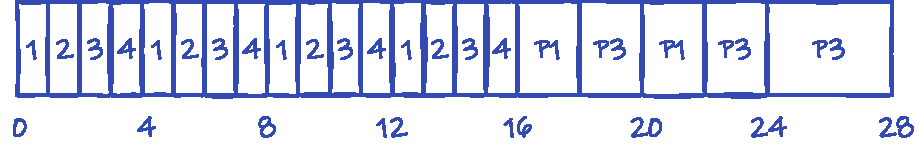
\includegraphics[width=0.8\textwidth]{media/C14_planificación/equitativo1.pdf}
\caption{}
\end{figure}

El algoritmo de \textbf{planificación equitativa} es muy similar al
algoritmo \textbf{RR}, pero en la \textbf{planificación equitativa} la
ventana de tiempo que finalmente se asigna a cada proceso se calcula
dinámicamente.

\subsubsection{Implementación
básica}\label{_implementaciuxf3n_buxe1sica}

Las implementaciones del algoritmo de \textbf{planificación equitativa}
suelen utilizar el concepto de \emph{tiempo virtual} para seguir la
pista de cuánto tiempo debe ejecutarse el proceso. Por ejemplo, en el
planificador de \{zircon\}\hyperref[Fuchsia-ZirconFairScheduler]{???}
---el \emph{microkernel} de \{google\_fuchsia\}--- cuando un proceso
\(P_i\) entra en la \textbf{cola de preparados}, en el PCB de dicho
proceso se actualizan dos tiempos:

\begin{itemize}
\item
  \textbf{Instante inicial \(t_(si)\)} de la ráfaga de CPU del proceso,
  en el \emph{tiempo virtual} de la CPU.
\item
  \textbf{Instante final \(t_(fi)\)} de la ráfaga de CPU del proceso, en
  el \emph{tiempo virtual} de la CPU.
\end{itemize}

Estos tiempos se dicen que están en \emph{tiempo virtual} de la CPU para
señalar que idealmente el proceso comenzaría su ejecución en \(t_(si)\)
y terminaría en \(t_(fi)\), aunque esto difícilmente va a ocurrir en la
realidad porque el tiempo de CPU hay que repartirlo entre los diferentes
procesos.

\{zircon\} es un \emph{microkernel} multihilo con modelo uno a uno, por
lo que su planificador trabaja con hilos. Es decir, las propiedades que
necesita el planificador para hacer su trabajo están vinculadas a los
hilos y son estos hilos los que el planificador ordena y selecciona para
ser ejecutados en la CPU. Sin embargo, en la versión que vamos a
describir hablaremos de planificar procesos, por coherencia con cómo
hemos explicado el resto de planificadores de este capítulo.

Si \(t\) es el instante de tiempo en el que un proceso \(P_i\) entra en
la cola de preparados, el instante inicial \(t_(si)\) y el instante
final \(t_(fi)\) se calculan de la siguiente manera:

\[{: (t_(si), =, t\qquad\qquad), (t_(fi), =, t_(si) + gM):}\]

donde \(M\) es la porción mínima de tiempo de CPU real que se puede
asignar a cada proceso y \(g\) es la cantidad de estas porciones de
tiempo que se quiere repartir entre todos los procesos que están en
disposición de ser ejecutados. Es decir, en el ejemplo anterior
\(gM = 4" ms"\), por lo que si la porción mínima fuera \(M = 1" ms."\),
cada periodo tendría 4 porciones de tiempo para repartir.

En la \textbf{cola de preparados} los procesos son ordenados por el
valor de \(t_(fi)\), de forma que primero se planifican los procesos que
tiene ráfagas que virtualmente terminarían antes.

El planificador de \{zircon\} tiene una serie de parámetros ajustables:

\begin{itemize}
\item
  La \textbf{granularidad mínima \(M\)} que, como hemos comentado, es la
  porción mínima de tiempo de CPU real que se puede asignar a cualquier
  proceso.
\item
  La \textbf{latencia objetivo \(L\)}, que es el periodo de tiempo de
  CPU mínimo que se va a repartir entre los procesos. Es decir, dentro
  de un periodo de \textbf{latencia objetivo} \(L\) hay
  \("floor"(L / M)\) porciones de tiempo para repartir entre los
  procesos.
\end{itemize}

Si hay \(n\) procesos que se pueden ejecutar, lo que hace el
planificador es calcular \(g\) de la siguiente manera:

\[g = max(n, "floor"(L/M))\]

de forma que siempre haya suficientes porciones \(M\) para que cada
proceso pueda tener al menos una, limitando por debajo el número de
porciones a repartir a \("floor"(L / M)\).

Cuando se escoge un proceso para su ejecución, se calcula el cuanto real
\(t_i\) durante el que se le asignará la CPU:

\[t_i = "ceil"(g/n)*M\]

de forma que se reparten las \(g\) porciones entre los \(n\) procesos.

Si hay muchos procesos, \(g = n\), por lo que a cada proceso se le
asigna un tiempo de CPU de \(M\). Si hay pocos procesos,
\(g = "floor"(L / M)\), por lo que a cada proceso se le asignan varias
porciones \(M\) de tiempo de CPU del periodo \(L\).

\subsubsection{Planificación equitativa
ponderada}\label{_planificaciuxf3n_equitativa_ponderada}

{} Al igual que en los algoritmos anteriores de planificación, en
ocasiones puede ser interesante priorizar unos procesos frente a otros,
tanto por motivos ajenos al sistema operativo como por motivos internos.
Por ejemplo, se puede querer favorecer a los procesos limitados por la
E/S para mejorar la eficiencia del sistema, tal y como comentamos en el
apartado \hyperref[_ciclo_de_ruxe1fagas_de_cpu_y_de_es]{Ciclo de ráfagas
de CPU y de E/S}.

La \textbf{planificación equitativa} resuelve este problema permitiendo
que a los procesos se les asignen pesos y repartiendo más tiempo de CPU
a los procesos con mayor peso. A esta generalización del planificador
equitativo se la conoce como \textbf{planificador equitativo ponderado}.

Linux, desde la versión 2.6.23, utiliza un tipo de \textbf{planificador
equitativo ponderado} denominado \textbf{{}CFS} (\emph{Completely Fair
Scheduler}) o \textbf{planificador completamente
equitativo}{}\hyperref[Jones2018]{???}. Otro ejemplo es \{zircon\} que,
como hemos comentado, está inmerso en cambiar su actual planificador
basado en colas multinivel con prioridades a una implementación del
\textbf{planificador equitativo} que, de hecho, es realmente un
\textbf{planificador equitativo
ponderado}\hyperref[Fuchsia-ZirconFairScheduler]{???}.

\subsubsection{Implementación de la planificación equitativa
ponderada}\label{_implementaciuxf3n_de_la_planificaciuxf3n_equitativa_ponderada}

En \{zircon\} cada proceso \(P_i\) tiene un peso \(w_i\) que indica la
importancia del proceso en el reparto del tiempo de CPU.

El primer cambio ---respecto a la implementación vista anteriormente---
es que el instante final \(t_(fi)\) realmente se calcula de la siguiente
manera:

\[t_(fi) = t_(si) + gM/w_i\]

de forma que es los procesos con mayor peso \(w_i\) tiene un \(t_(fi)\)
más pequeño, por lo que se colocan antes en la \textbf{cola de
preparados}.

Cuando se escoge un proceso para su ejecución, se calcula el cuanto real
\(t_(i)\) durante el que se le asignará la CPU, asignándole un tiempo
proporcional al peso del proceso \(w_i\) respecto al peso del resto de
los procesos con los que compite:

\[t_i = "ceil"(g*w_i/W)*M\]

donde \(W\) es la suma de todos los pesos \(w_i\) para los \(n\)
procesos preparados para ser ejecutados.

\subsubsection{Ejemplo de planificación equitativa
ponderada}\label{_ejemplo_de_planificaciuxf3n_equitativa_ponderada}

Ilustremos el algoritmo con un ejemplo con \(L=5\) y \(M=1\):

\begin{longtable}[]{@{}
  >{\raggedright\arraybackslash}p{(\linewidth - 6\tabcolsep) * \real{0.2500}}
  >{\raggedright\arraybackslash}p{(\linewidth - 6\tabcolsep) * \real{0.2500}}
  >{\raggedright\arraybackslash}p{(\linewidth - 6\tabcolsep) * \real{0.2500}}
  >{\raggedright\arraybackslash}p{(\linewidth - 6\tabcolsep) * \real{0.2500}}@{}}
\toprule\noalign{}
\begin{minipage}[b]{\linewidth}\centering
Proceso
\end{minipage} & \begin{minipage}[b]{\linewidth}\centering
Tiempo de llegada (ms)
\end{minipage} & \begin{minipage}[b]{\linewidth}\centering
Tiempo de ráfaga de CPU (ms)
\end{minipage} & \begin{minipage}[b]{\linewidth}\centering
Peso
\end{minipage} \\
\midrule\noalign{}
\endhead
\bottomrule\noalign{}
\endlastfoot
P1 & 0 & 10 & 2 \\
P2 & 1 & 2 & 1 \\
P3 & 2 & 3 & 2 \\
P4 & 3 & 2 & 5 \\
\end{longtable}

El resultado es el que se muestra en el siguiente diagrama de Gantt:

\begin{figure}
\centering
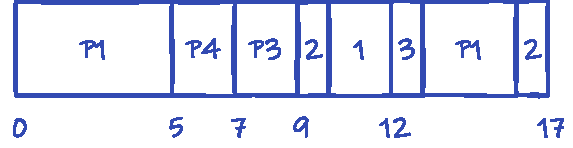
\includegraphics[width=0.8\textwidth]{media/C14_planificación/equitativo2.pdf}
\caption{}
\end{figure}

Al empezar, el primer proceso está solo cuando se le asigna la CPU, por
lo que puede consumir toda la latencia de planificación \(L\) en el
primer periodo. Posteriormente, cuando vuelve a la \textbf{cola de
preparados} en el instante 5, han llegado el resto de procesos, por lo
que tiene que competir con ellos por la CPU.

A partir de ese instante el orden para asignar la CPU viene determinado
por \(t_(fi)\), cuya expresión depende de \(g\). En este caso
\(g=M/L=5\) en todo momento, puesto que hay menos procesos que porciones
de tiempo \(M\) en \(L\).

En la siguiente tabla se puede observar los valores de \(t_(si)\) y
\(t_(fi)\) para cada proceso en el instante 5:

\begin{longtable}[]{@{}
  >{\raggedright\arraybackslash}p{(\linewidth - 4\tabcolsep) * \real{0.3333}}
  >{\raggedright\arraybackslash}p{(\linewidth - 4\tabcolsep) * \real{0.3333}}
  >{\raggedright\arraybackslash}p{(\linewidth - 4\tabcolsep) * \real{0.3333}}@{}}
\toprule\noalign{}
\begin{minipage}[b]{\linewidth}\centering
Proceso
\end{minipage} & \begin{minipage}[b]{\linewidth}\centering
\(t_(si)\)
\end{minipage} & \begin{minipage}[b]{\linewidth}\centering
\(t_(fi)\)
\end{minipage} \\
\midrule\noalign{}
\endhead
\bottomrule\noalign{}
\endlastfoot
P1 & 5 & 7.5 \\
P2 & 1 & 6 \\
P3 & 2 & 4.5 \\
P4 & 3 & 4 \\
\end{longtable}

Aunque el proceso \(P_4\) es el último en llegar, es el siguiente en ser
planificado, porque al tener un peso más alto su \(t_f4\) es el más
bajo. Entonces se calcula el tiempo de cuanto \(t_4\), que da 3, por lo
que se planifica en la CPU durante ese tiempo.

Sin embargo, \(P_4\) no consume su tiempo de cuanto porque su ráfaga
terminar antes, por lo que en el instante 7 se tiene que planificar el
siguiente proceso en la \textbf{cola de preparados}. En este caso sería
\(P_3\), con un tiempo de cuanto de 2.

Para calcular \(t_3\) es importante recordar que \(W = 5\), puesto que
\(P_4\) ya no está en la \textbf{cola de preparados} por lo que su peso
no se incluye.

En el instante 9, el proceso \(P_3\) es expulsado de la CPU y vuelve a
la \textbf{cola de preparados}. Entonces, se tienen que actualizar sus
valores para \(t_(si)\) y \(t_(fi)\) con el objeto de determinar cuál
será el próximo proceso planificado:

\begin{longtable}[]{@{}
  >{\raggedright\arraybackslash}p{(\linewidth - 4\tabcolsep) * \real{0.3333}}
  >{\raggedright\arraybackslash}p{(\linewidth - 4\tabcolsep) * \real{0.3333}}
  >{\raggedright\arraybackslash}p{(\linewidth - 4\tabcolsep) * \real{0.3333}}@{}}
\toprule\noalign{}
\begin{minipage}[b]{\linewidth}\centering
Proceso
\end{minipage} & \begin{minipage}[b]{\linewidth}\centering
\(t_(si)\)
\end{minipage} & \begin{minipage}[b]{\linewidth}\centering
\(t_(fi)\)
\end{minipage} \\
\midrule\noalign{}
\endhead
\bottomrule\noalign{}
\endlastfoot
P1 & 5 & 7.5 \\
P2 & 1 & 6 \\
P3 & 9 & 11.5 \\
\end{longtable}

Por tanto, el siguiente proceso a planificar es \(P_2\) con \(t_2 = 1\).
Y así se repite el procedimiento, sucesivamente.

Una vez resuelto el problema, los \textbf{tiempos de espera y ejecución
promedio} correspondientes serían:

\begin{longtable}[]{@{}
  >{\raggedright\arraybackslash}p{(\linewidth - 10\tabcolsep) * \real{0.2857}}
  >{\raggedright\arraybackslash}p{(\linewidth - 10\tabcolsep) * \real{0.1429}}
  >{\raggedright\arraybackslash}p{(\linewidth - 10\tabcolsep) * \real{0.1429}}
  >{\raggedright\arraybackslash}p{(\linewidth - 10\tabcolsep) * \real{0.1429}}
  >{\raggedright\arraybackslash}p{(\linewidth - 10\tabcolsep) * \real{0.1429}}
  >{\raggedright\arraybackslash}p{(\linewidth - 10\tabcolsep) * \real{0.1429}}@{}}
\toprule\noalign{}
\begin{minipage}[b]{\linewidth}\centering
Proceso
\end{minipage} & \begin{minipage}[b]{\linewidth}\centering
Instante de finalización (ms)
\end{minipage} &
\multicolumn{2}{>{\centering\arraybackslash}p{(\linewidth - 10\tabcolsep) * \real{0.2857} + 2\tabcolsep}}{\begin{minipage}[b]{\linewidth}\centering
Tiempo de espera (ms)
\end{minipage} &
\multicolumn{2}{>{\centering\arraybackslash}p{(\linewidth - 10\tabcolsep) * \real{0.2857} + 2\tabcolsep}@{}}{\begin{minipage}[b]{\linewidth}\centering
Tiempo de ejecución (ms)
\end{minipage} \\
\midrule\noalign{}
\endhead
\bottomrule\noalign{}
\endlastfoot
P1 & 16 & {(0-0) + (10-5) + (13-12)=} & 6 & {(16-0)=} & 16 \\
P2 & 17 & {(9-1) + (16-10)=} & 14 & {(17-1)=} & 16 \\
P3 & 14 & {(7-2) + (12-9)=} & 7 & {(13-2)=} & 11 \\
P4 & 7 & {(5-4)=} & 1 & {(7-3)=} & 4 \\
\end{longtable}

\subsection{Planificación con colas
multinivel}\label{_planificaciuxf3n_con_colas_multinivel}

{} Los diseñadores recurren a la \textbf{planificación de colas
multinivel} cuando quieren combinar las características de varios
algoritmos.

En la planificación con colas multinivel se divide la cola de preparados
en colas separadas. Los procesos son asignados permanentemente a alguna
de dichas colas, cada una de las cuales puede tener un algoritmo de
planificación distinto.

La asignación de un proceso a una cola se hace en relación a alguna una
característica del proceso. Por ejemplo, si es interactivo o no, su
prioridad o su tamaño en memoria. Se hace de esta manera porque se
supone que los procesos se pueden clasificar, y que cada clase tiene
diferentes requerimientos. Por ejemplo, si los procesos se clasifican en
interactivos o no interactivos, los primeros pueden ir a una cola con
planificación \textbf{RR} mientras los segundos van a una con
\textbf{FCFS}.

\begin{figure}
\centering
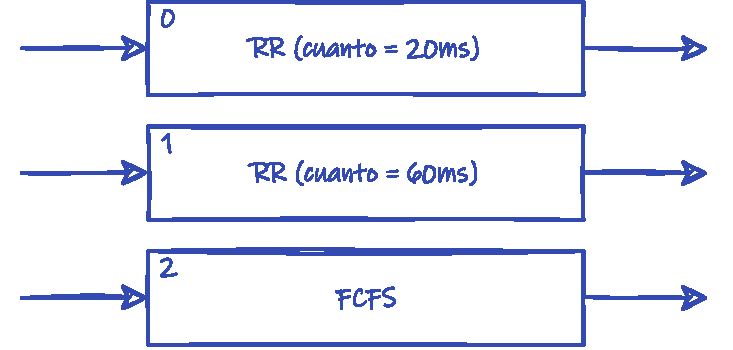
\includegraphics[width=0.8\textwidth]{media/C14_planificación/planificación_colas_multinivel.pdf}
\caption{Ejemplo de planificación con colas
multinivel.}\label{fig-colas-multinivel}
\end{figure}

Una cuestión interesante es cómo seleccionar la cola que debe escoger al
siguiente proceso a ejecutar:

\begin{itemize}
\item
  Una opción común en los sistemas actuales es utilizar un
  \textbf{planificador con prioridades}. Es decir, que cada cola tenga
  una prioridad y así el planificador solo tiene que escoger la cola de
  prioridad más alta que no esté vacía.

  Por ejemplo, en la \hyperref[fig-colas-multinivel]{Ejemplo de
  planificación con colas multinivel.}, mientras un proceso de prioridad
  1 esté preparado, no se escoge ningún otro de prioridad inferior. Si
  este planificador se implementa de forma expropiativa, el proceso que
  tiene asignada la CPU es expulsado si un proceso entra en una de las
  colas que tiene mayor prioridad que la suya.
\item
  Otra opción es usar cuantos sobre las colas. Es decir, que a cada cola
  se le asigne una porción del tiempo de la CPU que debe repartirse
  entre los distintos procesos en la misma.

  Por ejemplo, un 80\% de CPU para la cola de procesos interactivos, con
  planificación \textbf{RR}, y el 20\% de CPU restante para la cola de
  procesos no interactivos, con planificador \textbf{FCFS}.
\end{itemize}

La \textbf{planificación de colas multinivel} con un
\textbf{planificador con prioridades} para escoger la cola adecuada, es
con diferencia la opción más común en los sistemas operativos modernos.
Sin embargo, en este tipo de \textbf{colas multinivel} la asignación de
los procesos a las colas es permanente ---si la asignación se hace por
prioridad, significa que la prioridad es fija---. Mientras que hoy en
día es común que los procesos se muevan entre colas según las
características del proceso.

\subsection{Planificación con colas multinivel
realimentadas}\label{_planificaciuxf3n_con_colas_multinivel_realimentadas}

{} Para aumentar la flexibilidad de la planificación con colas
multinivel se puede permitir a los procesos pasar de una cola a otra.
Así se pueden clasificar en colas distintas, procesos con diferentes
tiempos de ráfaga de CPU. Por ejemplo, para situar los procesos
interactivos o limitados por la E/S en las colas de más alta prioridad,
lo que ya hemos discutido que mejora los tiempos de espera y de
respuesta y evita el \textbf{efecto convoy}.

\begin{figure}
\centering
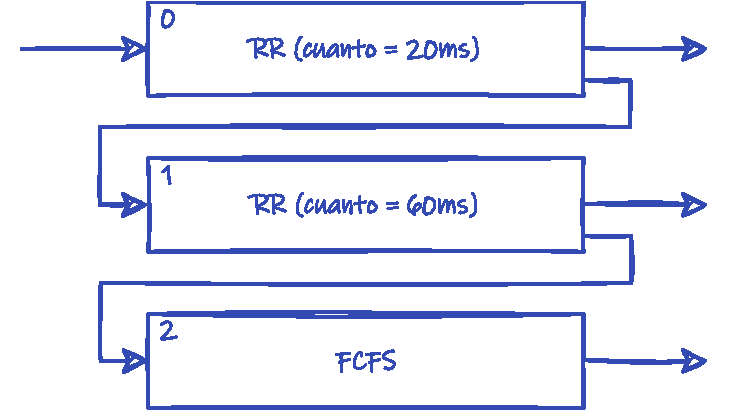
\includegraphics[width=0.8\textwidth]{media/C14_planificación/planificación_colas_multinivel_realimentadas.pdf}
\caption{Ejemplo de planificación con colas multinivel
realimentadas.}\label{fig-planificaciuxf3n-colas-multinivel-realimentadas}
\end{figure}

Por ejemplo, supongamos un \textbf{planificador de colas multinivel}
donde cada cola tiene una prioridad, así que se usa la
\textbf{planificación con prioridades} para seleccionar la cola. En las
colas se usa el algoritmo \textbf{RR} para seleccionar el siguiente
proceso, siendo el \textbf{cuanto} de la cola mayor cuanto menos
prioritaria es la cola (véase la
\hyperref[fig-planificaciuxf3n-colas-multinivel-realimentadas]{Ejemplo
de planificación con colas multinivel realimentadas.}). Los procesos que
llegan nuevos o desde el estado \textbf{esperando} lo hacen con la
prioridad más alta ---que por convención hemos decidido que sea 0--- así
que se insertan en la cola correspondiente. Mientras que los procesos
expropiados por vencimiento del \textbf{cuanto} pierde un punto de
prioridad, siendo insertados en una cola de prioridad menor.

Con este algoritmo los procesos limitados por E/S suelen ejecutarse la
mayor parte del tiempo con prioridades más altas que los limitados por
CPU. Por ejemplo, usando los valores del esquema de la
\hyperref[fig-planificaciuxf3n-colas-multinivel-realimentadas]{Ejemplo
de planificación con colas multinivel realimentadas.}, los procesos de
ráfagas de CPU entre 20 y 80 ms acaban cayendo a la cola de prioridad 1
tras 20 ms de ejecución. Así dejan paso a los procesos con ráfagas
menores de 20 ms, que siempre se ejecutan con prioridad 0. Finalmente,
los procesos de ráfagas mayores de 80 ms van a la cola FCFS, desde donde
solo tendrán acceso a la CPU cuando no haya ningún proceso de los otros
tipos en la \textbf{cola de preparados}

El \textbf{planificador de colas multinivel realimentadas} también se
puede utilizar para pasar a colas superiores los procesos que han
esperado mucho tiempo en colas inferiores, evitando la \textbf{muerte
por inanición}, que puede afectar a los sistemas de
\textbf{planificación de colas multinivel} con \textbf{prioridad fija}.

Por ejemplo, el algoritmo \textbf{RR virtual}{}{} es un caso de
\textbf{planificador de colas multinivel realimentadas} que resuelve los
problemas del \textbf{RR}, en cuanto al reparto de la CPU entre procesos
limitados por la E/S y limitados por la CPU (véase el
\hyperref[_reparto_equitativo_del_tiempo_de_cpu]{Reparto equitativo del
tiempo de CPU}).

\begin{figure}
\centering
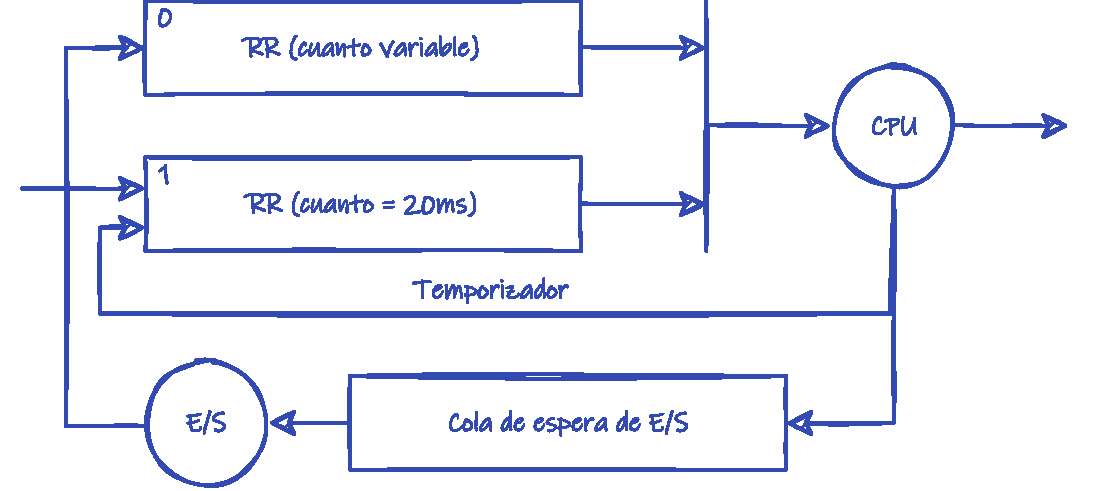
\includegraphics[width=0.8\textwidth]{media/C14_planificación/vrr.pdf}
\caption{Ejemplo de planificación con RR
virtual.}\label{fig-planificaciuxf3n-rr-virtual}
\end{figure}

Tal y como se ilustra en la
\hyperref[fig-planificaciuxf3n-rr-virtual]{Ejemplo de planificación con
RR virtual.}, en el \textbf{RR virtual} los procesos por lo general
tienen prioridad 1. Sin embargo, aquellos que vuelven al estado
\textbf{preparado} desde \textbf{esperando} después de una operación de
E/S, obtienen una bonificación en la propiedad que los lleva a tener
prioridad 0. Por tanto, los procesos que usan con más frecuencia la E/S,
usan más la cola de prioridad más alta, por lo que se les asigna antes
la CPU mayor frecuencia.

Esta solución puede llevar a que si hay muchos procesos limitados por la
E/S, estos acaparen la CPU y no den oportunidad de ejecutarse a los
procesos en la cola de prioridad 1. Para evitarlo, el algoritmo
\textbf{RR} de la cola de prioridad 0 tiene un \textbf{cuanto} variable,
de tal forma que cada proceso recibe lo que le queda del \textbf{cuanto}
de la cola de prioridad 1 tras haber consumido parte en la CPU en la
ráfaga anterior. Esto hace que incluso los procesos con ráfagas de CPU
más cortas acaben consumiendo su \textbf{cuanto} en la cola de prioridad
0 y terminen cayendo a la cola de prioridad 1, dando oportunidad de
ejecutarse a otros procesos.

Para ilustrar los visto hasta el momento sobre la planificación de la
CPU en sistemas operativos modernos, vamos a comentar las principales
características de las últimas versiones de Microsoft Windows a este
respecto.

Las actuales versiones de sistemas operativos Windows pertenecen a la
familia de Microsoft Windows NT; que nació con el sistema operativo
Windows NT 3.1 en 1993 y que llega hasta hoy en día con Microsoft
Windows 10 y Windows Server 2019 ---que se corresponden con la versión
10.0 de dicha familia Windows NT---

El núcleo de la familia Windows NT es multihilo e internamente
implementa un algoritmo de planificación expropiativa con colas
multinivel realimentadas basado en prioridades.

En Windows las prioridades de los hilos se pueden ver desde dos
perspectivas: la de Windows API y la del núcleo. Ambas tienen una
organización muy diferente, pero en última instancia, las primeras deben
traducirse en las segundas.

\begin{longtable}[]{@{}
  >{\raggedright\arraybackslash}p{(\linewidth - 2\tabcolsep) * \real{0.5000}}
  >{\raggedright\arraybackslash}p{(\linewidth - 2\tabcolsep) * \real{0.5000}}@{}}
\caption{Clases de prioridad en Windows
API.}\label{tabla-win32-clases-prioridad}\tabularnewline
\toprule\noalign{}
\begin{minipage}[b]{\linewidth}\centering
Clase
\end{minipage} & \begin{minipage}[b]{\linewidth}\centering
Valor
\end{minipage} \\
\midrule\noalign{}
\endfirsthead
\toprule\noalign{}
\begin{minipage}[b]{\linewidth}\centering
Clase
\end{minipage} & \begin{minipage}[b]{\linewidth}\centering
Valor
\end{minipage} \\
\midrule\noalign{}
\endhead
\bottomrule\noalign{}
\endlastfoot
REALTIME\_PRIORITY\_CLASS & 0x00000100 \\
HIGH\_PRIORITY\_CLASS & 0x00000080 \\
ABOVE\_NORMAL\_PRIORITY\_CLASS & 0x00008000 \\
NORMAL\_PRIORITY\_CLASS & 0x00000020 \\
BELOW\_NORMAL\_PRIORITY\_CLASS & 0x00004000 \\
IDLE\_PRIORITY\_CLASS & 0x00000040 \\
\end{longtable}

Desde el punto de vista de Windows API, todo proceso pertenece a alguna
de las 6 clases de prioridad de la
\hyperref[tabla-win32-clases-prioridad]{Clases de prioridad en Windows
API.}\hyperref[Win32-SchedulingPriorities]{???}. La clase de prioridad
de un proceso se puede indicar durante la creación del proceso, a través
del argumento \texttt{dwCreationFlags} de la función
\{win32\_createprocess\}, o sea puede obtener y cambiar con las
funciones \{win32\_getpriorityclass\} y \{win32\_setpriorityclass\},
respectivamente. Por lo general, la clase de prioridad
\texttt{NORMAL\_PRIORITY\_CLASS} es la clase por defecto de cualquier
proceso nuevo, excepto que se indique otra cosa durante su creación.

\begin{figure}
\centering
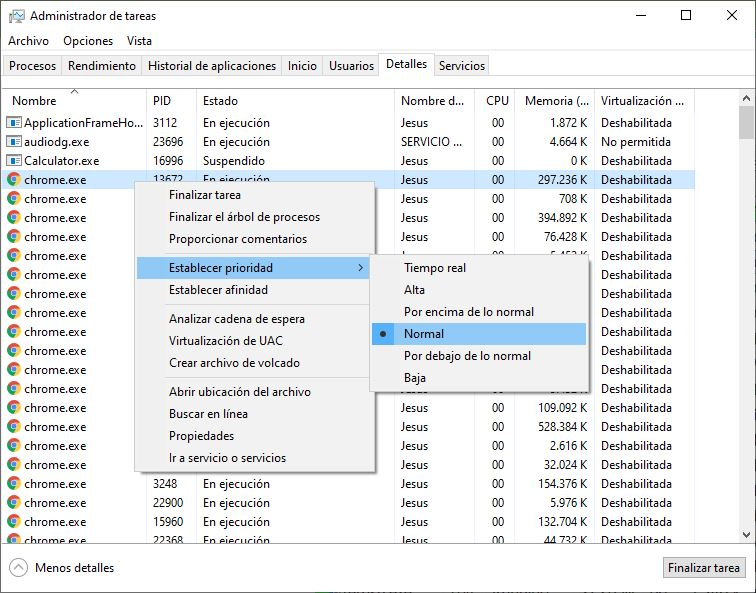
\includegraphics[keepaspectratio]{media/C14_planificación/administrador_de_tareas.jpg}
\caption{Cambiar la prioridad de un proceso en el \textbf{Administrador
de tareas}.}\label{fig-windows-task-manager}
\end{figure}

Con el \textbf{Administrador de tareas} de Windows podemos alterar
fácilmente la clase de prioridad de un proceso durante su ejecución
(véase la \hyperref[fig-windows-task-manager]{Cambiar la prioridad de un
proceso en el .}).

\begin{longtable}[]{@{}
  >{\raggedright\arraybackslash}p{(\linewidth - 2\tabcolsep) * \real{0.5000}}
  >{\raggedright\arraybackslash}p{(\linewidth - 2\tabcolsep) * \real{0.5000}}@{}}
\caption{Clases de prioridad en Windows
API.}\label{tabla-win32-prioridad-hilos}\tabularnewline
\toprule\noalign{}
\begin{minipage}[b]{\linewidth}\centering
Prioridad
\end{minipage} & \begin{minipage}[b]{\linewidth}\centering
Valor
\end{minipage} \\
\midrule\noalign{}
\endfirsthead
\toprule\noalign{}
\begin{minipage}[b]{\linewidth}\centering
Prioridad
\end{minipage} & \begin{minipage}[b]{\linewidth}\centering
Valor
\end{minipage} \\
\midrule\noalign{}
\endhead
\bottomrule\noalign{}
\endlastfoot
THREAD\_PRIORITY\_TIME\_CRITICAL & 15 \\
THREAD\_PRIORITY\_HIGHEST & 2 \\
THREAD\_PRIORITY\_ABOVE\_NORMAL & 1 \\
THREAD\_PRIORITY\_NORMAL & 0 \\
THREAD\_PRIORITY\_BELOW\_NORMAL & -1 \\
THREAD\_PRIORITY\_LOWEST & -2 \\
THREAD\_PRIORITY\_IDLE & 15 \\
\end{longtable}

Al mismo tiempo, cada hilo del sistema tiene alguno de las prioridades
de la \hyperref[tabla-win32-prioridad-hilos]{Clases de prioridad en
Windows API.}. La prioridad de un hilo recién creado es
\texttt{THREAD\_PRIORITY\_NORMAL}, pero se puede cambiar usando la
función \{win32\_setthreadpriority\}.

El núcleo de Windows tiene 32 prioridades, siendo 31 la prioridad más
alta y 0 la más baja. Estos valores se dividen en dos rangos. El rango
de prioridades de tiempo real va de 16 a 31 y solo está disponible para
hilos en procesos en la clase de prioridad
\texttt{REALTIME\_PRIORITY\_CLASS}. Mientras que el rango de prioridades
dinámicas va de 1 a 15. El nivel 0 está reservado para el sistema y se
usa para una rutina especializada en limpiar zonas de memoria liberada
por los procesos, poniéndolas a 0.

La prioridad base ---o prioridad estática--- de cada hilo que ve el
núcleo se calcula combinando la prioridad del hilo y la clase de
prioridad del proceso al que pertenece.

\begin{longtable}[]{@{}
  >{\raggedright\arraybackslash}p{(\linewidth - 12\tabcolsep) * \real{0.1429}}
  >{\raggedright\arraybackslash}p{(\linewidth - 12\tabcolsep) * \real{0.1429}}
  >{\raggedright\arraybackslash}p{(\linewidth - 12\tabcolsep) * \real{0.1429}}
  >{\raggedright\arraybackslash}p{(\linewidth - 12\tabcolsep) * \real{0.1429}}
  >{\raggedright\arraybackslash}p{(\linewidth - 12\tabcolsep) * \real{0.1429}}
  >{\raggedright\arraybackslash}p{(\linewidth - 12\tabcolsep) * \real{0.1429}}
  >{\raggedright\arraybackslash}p{(\linewidth - 12\tabcolsep) * \real{0.1429}}@{}}
\caption{Clases de prioridad base en Windows
API.}\label{tabla-win32-prioridad-estuxe1tica}\tabularnewline
\toprule\noalign{}
\endfirsthead
\endhead
\bottomrule\noalign{}
\endlastfoot
&
\multicolumn{6}{>{\centering\arraybackslash}p{(\linewidth - 12\tabcolsep) * \real{0.8571} + 10\tabcolsep}@{}}{\textbf{Clase de prioridad del proceso}} \\
& \textbf{REALTIME} & \textbf{HIGH} & \textbf{ABOVE NORMAL} &
\textbf{NORMAL} & \textbf{BELOW NORMAL} & \textbf{IDLE} \\
\textbf{TIME CRITICAL} & 31 & 15 & 15 & 15 & 15 & 15 \\
\textbf{HIGHEST} & 26 & 15 & 12 & 10 & 8 & 6 \\
\textbf{ABOVE NORMAL} & 25 & 15 & 11 & 9 & 7 & 6 \\
\textbf{NORMAL} & 24 & 13 & 10 & 8 & 6 & 4 \\
\textbf{BELOW NORMAL} & 23 & 12 & 9 & 7 & 5 & 3 \\
\textbf{LOWEST} & 22 & 11 & 8 & 6 & 4 & 2 \\
\textbf{IDLE} & 16 & 1 & 1 & 1 & 1 & 1 \\
\end{longtable}

Esta prioridad base es la prioridad real del hilo, si este tiene una
prioridad en el rango de tiempo real ---es decir, si el proceso al que
pertenece está en la clase de prioridad
\texttt{REALTIME\_PRIORITY\_CLASS}---. Mientras que para el resto de
hilos, el sistema suma ciertas bonificaciones a la prioridad base para
calcular la prioridad dinámica, que es con la que realmente será
planificado el hilo. Estas bonificaciones se truncan para que nunca
puedan hacer que el hilo se meta en el rango de tiempo real.

La prioridad real la usa el sistema para determinar a qué cola va el
hilo cuando va a ser insertado en la \textbf{cola de preparados}. Para
cada nivel de prioridad hay una cola con algoritmo \textbf{RR}, de tal
forma que el planificador escoge primero a los hilos con prioridad más
alta. Dentro de la misma prioridad la CPU se asigna en turno, dándoles
un \textbf{cuanto} de tiempo de CPU.

Cuando llega un hilo a la cola de preparados, expropia la CPU al hilo
que la tiene asignada si este tiene menor prioridad. Esto puede ocurrir
incluso si el hilo a expropiar está en medio de una llamada al sistema,
ya que, como cualquier sistema operativo moderno, el núcleo de Windows
es expropiable ---lo que veremos en el
\hyperref[_nuxfacleo_expropiable]{Núcleo expropiable} que ofrece
latencias de asignación más bajas que si no lo fuera---.

Respecto al \textbf{cuanto}, desde Windows Vista --NT 6.0-- no se usa el
temporizador para controlarlo sino el contador de ciclos de reloj de la
CPU. Así el sistema puede determinar con precisión el tiempo que se ha
estado ejecutando un hilo, excluyendo los tiempos dedicados a otras
cuestiones, como por ejemplo a manejar interrupciones.

Desde el Intel Pentium las CPU de la familia x86 incorporan un contador
de marca de tiempo (\emph{Time Stamp Counter} o TSC) de 64 bits que
indica el número de ciclos transcurridos desde el último reinicio del
procesador\hyperref[Wikipedia-TSC]{???}.

Una característica curiosa es que los hilos expropiados se insertan en
la cabeza de su cola ---no en el final--- y conservan lo que les queda
de \textbf{cuanto}. Mientras que se insertan por el final con el valor
de \textbf{cuanto} reiniciado cuando abandonan la CPU por haber agotado
el cuanto anterior. Estos últimos, además, pierden un nivel de prioridad
si se ejecutaban con una prioridad superior a su prioridad base, a causa
de alguna modificación.

Las bonificaciones a los hilos en el rango de prioridades dinámicas
vienen determinadas por distintos criterios, escogidos para mejorar el
\textbf{tiempo respuesta} y el \textbf{tiempo de espera} ---priorizando
los procesos limitados por E/S--- evitar la \textbf{muerte por
inanición} y la \textbf{inversión de prioridad}.

Se bonifican los hilos que despiertan tras completar operaciones de E/S
con una cantidad que depende del tipo de dispositivo. Por ejemplo, la
bonificación es mejor para hilos que han esperado por el teclado o el
ratón que para los que esperaron por dispositivos del almacenamiento.
También son bonificados los hilos que despiertan de eventos, semáforos y
de otros objetos de sincronización. En este último caso, incluso se les
ofrece más tiempo de \textbf{cuanto} si es el hilo asociado a la ventana
de primer plano, con el objetivo de mejorar la respuesta de las
aplicaciones interactivas. También se bonifica cualquier hilo que
gestione elementos de la interfaz gráfica cuando despierta para
responder a eventos del sistema de ventanas.

Para evitar la \textbf{muerte por inanición}, el planificador escoge
cada segundo unos pocos hilos que llevan esperando aproximadamente 4
segundos, les triplica el \textbf{cuanto} y les aumenta la prioridad a
15. Estos hilos recuperan su prioridad base y el cuanto anterior cuando
agotan el tiempo de cuanto actual o son expropiados de la CPU

\section{Planificación de tiempo
real}\label{_planificaciuxf3n_de_tiempo_real}

En el \hyperref[_sistemas_de_tiempo_real]{???} discutimos la importancia
de los sistemas de tiempo real. A continuación, describiremos las
funcionalidades necesarias para soportar la ejecución de procesos en
tiempo real dentro de un sistema operativo de propósito general.

\subsection{Tiempo real estricto}\label{_tiempo_real_estricto}

{} {} {} Los sistemas de \textbf{tiempo real estricto} son necesarios
para realizar tareas críticas que deben ser completadas dentro de unos
márgenes de tiempo preestablecidos.

Generalmente las tareas son entregadas al sistema operativo junto con
una declaración de las restricciones de tiempo ---periodicidad y límite
de tiempo--- y la cantidad de tiempo que necesitan para ejecutarse. El
planificador solo admitirá las tareas si puede garantizar el
cumplimiento de las restricciones de tiempo, rechazándolas en caso
contrario.

El ofrecer estas garantías requiere que el planificador conozca
exactamente el tiempo máximo que se tarda en realizar todas y cada una
de las funciones del sistema operativo. Esto es imposible en sistemas
con almacenamiento secundario o memoria virtual, ya que introducen
variaciones no controladas en la cantidad de tiempo necesario para
ejecutar una tarea. Por tanto, el \textbf{tiempo real estricto} no es
compatible con los sistemas operativos de propósito general, como los
sistemas operativos de escritorio modernos.

\subsection{Tiempo real flexible}\label{_tiempo_real_flexible}

{} {} {} La ejecución de procesos de \textbf{tiempo real flexible} es
menos restrictiva. Tan solo requiere que los procesos críticos reciban
mayor prioridad que los que no lo son. Esto puede generar excesos en la
cantidad de recursos asignados a los procesos de tiempo real, así como
inanición y grandes retrasos en la ejecución del resto de los procesos,
pero es compatible con los sistemas de propósito general.

Además nos permite conseguir sistemas de propósito general que soporten
multimedia, videojuegos y otras tareas que no funcionan de manera
aceptable en un entorno que no implementara tiempo real flexible. Por
ello, la mayor parte de los sistemas operativos modernos soportan este
tipo de tiempo real.

\subsection{Implementación del soporte de tiempo
real}\label{_implementaciuxf3n_del_soporte_de_tiempo_real}

Implementar el soporte de tiempo real flexible en un sistema operativo
de propósito general requiere:

\begin{itemize}
\item
  \textbf{Sistema operativo con planificación con prioridades}. Los
  procesos de tiempo real deben tener la mayor prioridad y ser fija. Es
  decir, no deben ser afectados por ningún mecanismo de envejecimiento o
  bonificación, que pueda usarse con los procesos de tiempo no real.
\item
  \textbf{Baja latencia de asignación}. Cuanto menor es la latencia, más
  rápido comenzará a ejecutarse el proceso de tiempo real después de ser
  seleccionado por el planificador de la CPU.
\end{itemize}

Mientras que el primer requerimiento es bastante sencillo de conseguir,
el segundo es mucho más complejo.

\subsection{Reducir la latencia de
asignación}\label{_reducir_la_latencia_de_asignaciuxf3n}

Muchos sistemas operativos tienen un núcleo no expropiable. Estos
núcleos no pueden realizar un cambio de contexto mientras se está
ejecutando código del núcleo ---por ejemplo, debido a una llamada al
sistema--- por lo que se ven obligados a esperar hasta que la operación
que se esté realizando termine, antes de asignar la CPU a otro proceso.
Esto aumenta la \textbf{latencia de asignación}, dado que algunas
llamadas al sistema pueden ser muy complejas y requerir mucho tiempo
para completarse.

Con el objetivo de resolver este problema se han desarrollado diversas
alternativas para que el código del núcleo sea expropiable.

\subsubsection{Puntos de expropiación}\label{_puntos_de_expropiaciuxf3n}

Una posibilidad es introduciendo \textbf{puntos de expropiación}{} en
diversos lugares «seguros» dentro del código. En dichos puntos se
comprueba si algún proceso de prioridad más alta está en la cola de
preparados. En caso de que sea así, se expropia la CPU al proceso actual
y se le asigna al proceso de más alta prioridad.

Debido a la función que realizan los puntos de expropiación, solo pueden
ser colocados en lugares seguros del código del núcleo. Es decir,
lugares donde no se interrumpe la modificación de estructuras de datos.
Sin embargo, esto limita el número de puntos que pueden ser colocados,
por lo que la latencia de asignación puede seguir siendo muy alta para
algunas operaciones muy complejas del núcleo.

\subsubsection{Núcleo expropiable}\label{_nuxfacleo_expropiable}

Otra posibilidad es diseñar un \textbf{núcleo completamente
expropiable}.

Puesto que en este caso la ejecución de cualquier operación en el núcleo
puede ser interrumpida en cualquier momento por procesos de mayor
prioridad que el que actualmente tiene asignada la CPU, es necesario
proteger las estructuras de datos del núcleo con mecanismos de
sincronización. Esto hace que el diseño de un núcleo de estas
características sea mucho más complejo.

Microsoft Windows ---desde Windows NT--- Linux ---desde la versión
2.6--- \{solaris\} y \{netbsd\} son algunos ejemplos de sistemas
operativos con núcleos expropiables. En el caso concreto de Solaris la
latencia de asignación es inferior a 1 ms, mientras que con la
expropiación del núcleo desactivada esta puede superar los 100 ms

Lamentablemente, conseguir baja latencia de asignación no tiene coste
cero. El hecho de que el núcleo sea expropiable aumenta el número de
cambios de contexto, lo que reduce el rendimiento del sistema a cambio
de un menor tiempo de respuesta. Esto resulta muy interesante para
aplicaciones de tiempo real, multimedia y sistemas de escritorio, pero
es poco adecuado para servidores y computación de altas prestaciones.

Por eso desde Linux 2.6 se puede compilar el núcleo con diferentes
niveles, de lo expropiable que es el núcleo.

En la configuración por defecto \texttt{PREEMPT\_NONE}, el núcleo tiene
algunos \textbf{puntos de expropiación}, de tal forma que es ideal para
servidores y sistemas cómputo de altas prestaciones. Con
\texttt{PREEMPT\_VOLUNTARY} ---el siguiente nivel--- se añaden muchos
más \textbf{puntos de expropiación} con el objeto de reducir la
latencia, mejorando el tiempo de respuesta en sistemas de escritorio.

Finalmente, activando \texttt{PREEMPT} el núcleo se vuelve
\textbf{completamente expropiable} ---excepto en algunas secciones
críticas---. Esto es ideal para sistemas de escritorio o sistemas
empotrados con requisitos de latencia en el rango de los milisegundos.

\paragraph{Inversión de prioridad}\label{_inversiuxf3n_de_prioridad}

Supongamos que en un núcleo completamente expropiable, un proceso de
baja prioridad es interrumpido porque hay un proceso de alta prioridad
en la cola de preparados. Y que esto ocurre mientras el primero accede a
una importante estructura de datos del núcleo.

Durante su ejecución, el proceso de alta prioridad podría intentar
acceder a la misma estructura que trataba de manipular el proceso de
baja prioridad cuando fue interrumpido. Debido al uso de mecanismos de
sincronización, el proceso de alta prioridad se quedaría bloqueado y
tendría que abandonar la CPU a la espera de que el de baja, libere el
acceso al recurso. Sin embargo, este último tardará en ser asignado a la
CPU mientras haya algún otro proceso de alta prioridad en la cola de
preparados.

Al hecho de que un proceso de alta prioridad tenga que esperar por uno
de baja se le conoce como \textbf{{}inversión de la prioridad}. Para
resolverlo se utiliza un \textbf{{}protocolo de herencia de la
prioridad}, donde un proceso de baja prioridad hereda la prioridad del
proceso de más alta prioridad que espera por un recurso al que el
primero está accediendo. En el momento en que el proceso de baja
prioridad libere el acceso a dicho recurso, su prioridad retornará a su
valor original.

\section{Planificación en sistemas
multiprocesador}\label{_planificaciuxf3n_en_sistemas_multiprocesador}

Para tratar el problema de la planificación en los sistemas
multiprocesador nos limitaremos al caso de los \textbf{sistemas
homogéneos}{}. En dichos sistemas los procesadores son idénticos, por lo
que, en cualquiera de ellos, puede ejecutar cualquier proceso. Esto es
bastante común y simplifica el problema de la planificación.

Un ejemplo de lo contrario a un sistema homogéneo ---un sistema
heterogéneo--- se puede observar en los PC modernos, donde muchos
disponen tanto de una CPU como de una GPU, especializada en el
procesamiento de gráficos y en las operaciones vectoriales con números
enteros y de coma flotante.

Aun así, no debemos olvidar que incluso en el caso de los sistemas
homogéneos pueden aparecer limitaciones en la planificación. Por
ejemplo, los procesadores SMT (\emph{Simultaneous Multithreading})
permiten la ejecución concurrente de varios hilos de ejecución como si
de varias CPU se tratara. Sin embargo, al no disponer cada hilo de una
CPU completa, es posible que algunos debán esperar a que algún otro
libere unidades de ejecución de la CPU que le son necesarias. Eso debe
ser tenido en cuenta por el planificador con el fin de optimizar el
rendimiento del sistema.

La tecnología \emph{Hyper-threading} disponible en algunos procesadores
de Intel es una implementación de la tecnología \emph{Simultaneous
Multithreading}. Permite que cada núcleo de procesador que está presente
físicamente, el sistema operativo lo gestione como dos núcleos virtuales
---o lógicos--- y repartir entre ellos las tareas cuando es posible.

Al margen de estas cuestiones, según el tipo de procesamiento, existen
diversas posibilidades a la hora de enfrentar el problema de la
planificación en un sistema multiprocesador (véase el
\hyperref[_sistemas_multiprocesador]{???}).

\subsection{Multiprocesamiento
asimétrico}\label{_multiprocesamiento_asimuxe9trico}

{} {} Cuando utilizamos \textbf{multiprocesamiento asimétrico} todas las
decisiones de planificación, procesamiento de E/S y otras actividades
son gestionadas por el núcleo del sistema ejecutándose en un único
procesador: el \textbf{servidor} o \textbf{maestro}. El resto de
procesadores se limitan a ejecutar código de usuario, que les es
asignado por ese procesador \textbf{maestro}.

Este esquema es sencillo, puesto que evita la necesidad de compartir
estructuras de datos entre el código que se ejecuta en los diferentes
procesadores.

\subsection{Multiprocesamiento
simétrico}\label{_multiprocesamiento_simuxe9trico}

{} {} Cuando utilizamos \textbf{multiprocesamiento simétrico} o
\textbf{SMP}, cada procesador ejecuta su propia copia del núcleo del
sistema operativo y se autoplanifica mediante su propio planificador de
CPU. En estos sistemas nos podemos encontrar con varias alternativas.

\subsubsection{Con una cola de preparados
común}\label{_con_una_cola_de_preparados_comuxfan}

Algunos sistemas disponen de una cola de preparados común para todos los
procesadores. Puesto que se mira en una única cola, todos los procesos
pueden ser planificados en cualquier procesador.

Este esquema requiere el uso mecanismos de sincronización para controlar
el acceso concurrente de los núcleos a las colas. En caso contrario,
varios procesadores podrían escoger y ejecutar el mismo proceso a la
vez.

Muchos sistemas operativos modernos implementan el esquema SMP con una
cola de preparados común. Esto incluye Microsoft Windows NT/2000/XP,
Solaris, macOS y versiones anteriores a Linux 2.6.

Es importante recordar que en esos sistemas operativos, lo que se
planifica en las distintas CPU usando alguna de estas estrategias, son
los hilos y no los procesos.

Sin embargo, esta solución presenta algunos inconvenientes:

\begin{itemize}
\item
  La posibilidad de que un proceso se pueda ejecutar en cualquier CPU
  ---aunque parezca beneficiosa--- es negativa desde el punto de vista
  de que dejan de ser útiles las cachés de los procesadores, penalizando
  notablemente el rendimiento del sistema. Por eso, la mayoría de los
  sistemas operativos de este tipo evitan, en lo posible, la migración
  de procesos de un procesador a otro. A esto se lo conoce como asignar
  al proceso \textbf{{}afinidad al procesador}.
\item
  Los mecanismos de sincronización requeridos para controlar el acceso a
  la cola de preparados pueden mantener a los procesadores mucho tiempo
  desocupados ---mientras esperan--- en sistemas con un gran número de
  procesadores y con muchos procesos en la cola de preparados.
\end{itemize}

\subsubsection{Con una cola para cada
procesador}\label{_con_una_cola_para_cada_procesador}

Cada vez más sistemas modernos están optando por utilizar el esquema SMP
con una cola de preparados por procesador. De esta manera, al no
utilizar mecanismos de sincronización, se eliminan los tiempos de espera
para acceder a la cola de preparados y escoger un nuevo proceso.

El mayor inconveniente de esta solución es que puede generar
desequilibrios entre los procesadores, ya que un procesador puede acabar
desocupado ---con su cola de preparados vacía--- mientras otro está muy
ocupado. Con el fin de que esto no suceda, es necesario que el sistema
disponga de algunos mecanismos de \textbf{balanceo de carga}:

\begin{itemize}
\item
  En la \textbf{migración comandada}{} o \emph{push migration}, una
  tarea específica ---que se ejecuta con menor frecuencia que el
  planificador de la CPU--- estima la carga de trabajo de cada CPU y en
  caso de encontrar algún desequilibrio mueve algunos procesos de la
  cola de preparados de unos procesadores a la de los otros.
\item
  En la \textbf{migración solicitada}{} o \emph{pull migration}, un
  procesador inactivo extrae de la cola de preparados de un procesador
  ocupado alguna tarea que esté esperando.
\end{itemize}

Tanto el planificador de Linux 2.6 y posteriores, como el planificador
ULE de FreeBSD, implementan ambas técnicas. Mientras que en Microsoft
Windows, a partir de Windows Vista también se utiliza una cola de
preparados por procesador, pero solo implementa la \textbf{migración
solicitada}.


% ── Parte IV: Gestión de la memoria ──────────────────────
\part{Gesti\'{o}n de la memoria}
\input{partes/P04_preambulo}
\section{}

\textbf{Tiempo de lectura:} \{s15-reading-time\}

La memoria es un recurso central para el funcionamiento de un sistema
operativo moderno, puesto que es el único medio de almacenamiento al que
la CPU puede acceder directamente. Por ello, para que un programa pueda
ser ejecutado, debe ser cargado en la memoria desde el disco y creadas o
modificadas las estructuras internas del sistema operativo necesarias
para convertirlo en un proceso. Además, dependiendo de la forma en la
que se gestiona la memoria, los procesos ---o partes de los mismos---
pueden moverse de la memoria al disco ---y viceversa--- durante su
ejecución, con el objetivo de ajustar las necesidades de memoria para
mantener el \textbf{uso de la CPU} lo más alto posible.

Como comentamos en el \hyperref[_sistemas_multiprogramados]{???}, en los
\textbf{sistemas multiprogramados} existe una \textbf{cola de entrada},
que se define como aquella formada por el conjunto de procesos en disco
que esperan para ser cargados en la memoria para su ejecución.

Por tanto, el procedimiento normal de ejecución de un programa en dichos
sistemas es:

\begin{enumerate}
\def\labelenumi{\arabic{enumi}.}
\item
  Seleccionar un proceso de la cola de entrada y cargarlo en la memoria.
\item
  Mientras el proceso se ejecuta, este accede a instrucciones y datos de
  la memoria.
\item
  Finalmente, el proceso termina y su espacio en memoria es marcado como
  disponible.
\end{enumerate}

En los sistemas de propósito general modernos ---desde los
\textbf{sistemas de tiempo compartido} y los primeros \textbf{sistemas
de escritorio}--- no existe \textbf{cola de entrada}, por lo que los
programas se cargan inmediatamente en memoria cuando los usuarios
solicitan su ejecución. Excepto por eso, el procedimiento normal de
ejecución de un programa es similar al de los \textbf{sistemas
multiprogramados}.

\section{Etapas de un programa de
usuario}\label{_etapas_de_un_programa_de_usuario}

En la mayor parte de los casos, un programa de usuario debe pasar por
diferentes etapas ---algunas de las cuales son opcionales--- antes de
ser ejecutado (véase la
\hyperref[fig-etapas-programas-de-usuario]{Etapas de procesamiento de un
programa de usuario.}).

\begin{figure}
\centering
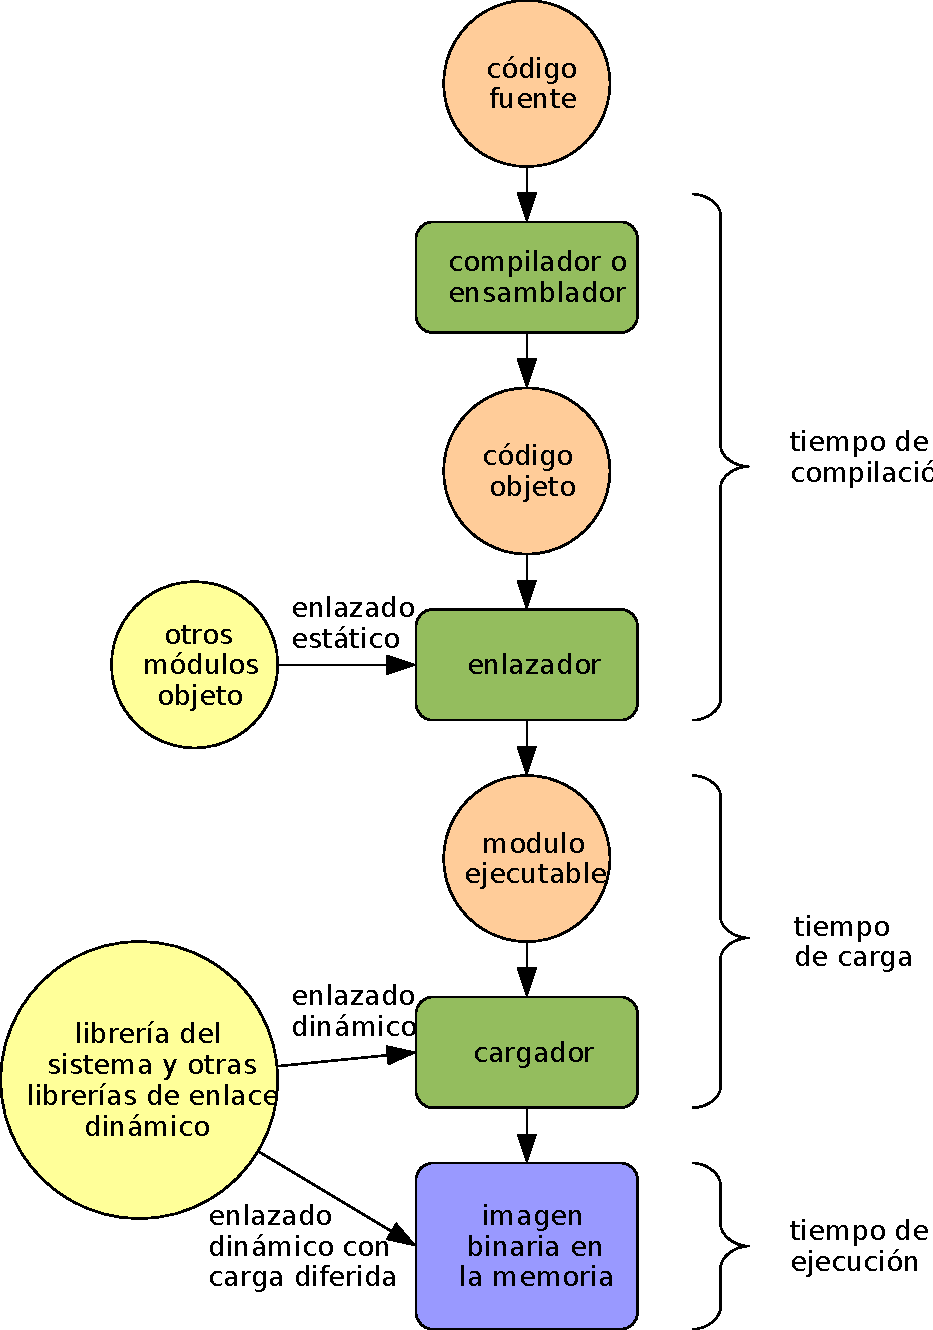
\includegraphics[width=0.8\textwidth]{media/C15_memoria_principal/etapas_de_un_programa_de_usuario.pdf}
\caption{Etapas de procesamiento de un programa de
usuario.}\label{fig-etapas-programas-de-usuario}
\end{figure}

Los archivos de \textbf{código fuente}{} del programa son compilados por
el compilador, generando un archivo de
\href{https://es.wikipedia.org/wiki/C\%C3\%B3digo_objeto}{\textbf{código
objeto}} ---con extensiones \texttt{.o} u \texttt{.obj}--- para cada
uno.

Todos los archivos de \textbf{código objeto}{} son unidos por el
enlazador para crear el archivo \textbf{ejecutable}, en una fase que se
denomina \textbf{enlazado estático}{}. En esta fase también se pueden
incorporar al ejecutable \textbf{librerías de enlace estático}{} ---con
extensiones \texttt{.a} o \texttt{.lib}--- con \textbf{código objeto}
que ha sido empaquetado para ser reutilizado en múltiples ejecutables.

El compilador y el enlazador suelen ser dos programas independientes,
aunque en ocasiones el compilador se haga cargo de ambas fases por
comodidad. Por ejemplo, en los sistemas GNU el compilador \{cmd\_gcc\}
por defecto genera el \textbf{código objeto} en archivos temporales,
luego invoca al enlazador \{cmd\_ld\} para crear el \textbf{ejecutable}
y finalmente elimina los archivos temporales.

En proyectos grandes suele ser más interesante usar ambas herramientas
por separado para reducir el tiempo de compilación. El compilador genera
los archivos de \textbf{código objeto}, que se conservan entre
compilaciones. Así, cada vez que se quiere generar una nueva versión del
ejecutable, solo es necesario compilar los archivos de \textbf{código
fuente} que hayan cambiado y luego enlazar juntos todos los archivos de
\textbf{código objeto}.

Al crear el \textbf{ejecutable} se pueden guardar en él dependencias
respecto a librerías que se enlazarán posteriormente, durante la carga o
ejecución del programa, en una fase denominada \textbf{enlazado
dinámico}{}.

En el momento en el que se va a ejecutar el programa, cuando está
construyendo la imagen binaria del proceso en la memoria; el sistema
operativo examina estas dependencias, carga las \textbf{librerías de
enlace dinámico}{} indicadas ---con extensiones \texttt{.so},
\texttt{dylib} o \texttt{.dll}--- y resuelve las referencias del
programa sus variables y funciones. Las \textbf{librerías de enlace
dinámico} contienen \textbf{código objeto}, enlazado en un formato
especial de \textbf{ejecutable} diseñado para contener partes
compartidas entre archivos ejecutables.

Este proceso puede ocurrir mientras se carga el \textbf{ejecutable}
---como se ha descrito--- o cuando el programa usa por primera vez un
elemento de las \textbf{librerías de enlace dinámico}. También es común
que el sistema ofrezca funciones para que los programas puedan cargar
manualmente e invocar funciones de \textbf{librerías de enlace
dinámico}. Esto es muy útil para crear programas que se puedan mejorar
por medio de extensiones o \emph{plugins}.

\begin{longtable}[]{@{}
  >{\raggedright\arraybackslash}p{(\linewidth - 6\tabcolsep) * \real{0.2500}}
  >{\raggedright\arraybackslash}p{(\linewidth - 6\tabcolsep) * \real{0.2500}}
  >{\raggedright\arraybackslash}p{(\linewidth - 6\tabcolsep) * \real{0.2500}}
  >{\raggedright\arraybackslash}p{(\linewidth - 6\tabcolsep) * \real{0.2500}}@{}}
\caption{Extensiones de archivos de programas.}\tabularnewline
\toprule\noalign{}
\begin{minipage}[b]{\linewidth}\raggedright
\end{minipage} & \begin{minipage}[b]{\linewidth}\raggedright
UNIX, Linux y otros sistemas estilo UNIX
\end{minipage} & \begin{minipage}[b]{\linewidth}\raggedright
macOS
\end{minipage} & \begin{minipage}[b]{\linewidth}\raggedright
Microsoft Windows
\end{minipage} \\
\midrule\noalign{}
\endfirsthead
\toprule\noalign{}
\begin{minipage}[b]{\linewidth}\raggedright
\end{minipage} & \begin{minipage}[b]{\linewidth}\raggedright
UNIX, Linux y otros sistemas estilo UNIX
\end{minipage} & \begin{minipage}[b]{\linewidth}\raggedright
macOS
\end{minipage} & \begin{minipage}[b]{\linewidth}\raggedright
Microsoft Windows
\end{minipage} \\
\midrule\noalign{}
\endhead
\bottomrule\noalign{}
\endlastfoot
\textbf{Código objeto} & \texttt{.o} & \texttt{.o} & \texttt{.obj} \\
\textbf{Librería de enlace estático} & \texttt{.a} & \texttt{.a} &
\texttt{.lib} \\
\textbf{Ejecutable} & & & \texttt{.exe} \\
\textbf{Librería de enlace dinámico} & \texttt{.so} & \texttt{.so},
\texttt{.dylib} & \texttt{.dll} \\
\textbf{Formato de ejecutables y librerías de enlace dinámico} &
\href{https://es.wikipedia.org/wiki/Executable_and_Linkable_Format}{Executable
and Linkable Format} (ELF) &
\href{https://en.wikipedia.org/wiki/Mach-O}{Mach-O} &
\href{https://es.wikipedia.org/wiki/Portable_Executable}{Portable
Executable} (PE) \\
\end{longtable}

\section{Reubicación de las
direcciones}\label{_reubicaciuxf3n_de_las_direcciones}

La mayor parte de los sistemas permiten que un proceso de usuario resida
en cualquier parte de la memoria física. Así, aunque el espacio de
direcciones del sistema comience en \texttt{0x00000000}, la primera
dirección del proceso de usuario no tiene por qué ser esa.

En cada una de las etapas vistas en el
\hyperref[_etapas_de_un_programa_de_usuario]{Etapas de un programa de
usuario} las direcciones pueden representarse de formas distintas, por
lo que en cada paso es necesario reasignar las direcciones usadas en una
etapa en direcciones de la siguiente.

Por ejemplo, en el código fuente de un programa las direcciones son
generalmente simbólicas, como los nombres de las variables y las
funciones. A continuación, un compilador suele reasignar esas
direcciones simbólicas en \textbf{direcciones reubicables}{} del estilo
de «120 bytes desde el comienzo del módulo». Finalmente ---el
enlazador--- que genera el ejecutable--- o el cargador ---que carga el
programa en la memoria--- convierte esas \textbf{direcciones
reubicables} en \textbf{direcciones absolutas}{}, como
\texttt{0x00210243}.

Por tanto, en cada etapa se traducen las direcciones de un espacio de
direcciones en el siguiente. Sin embargo, para que al final el programa
pueda ser ejecutado, es necesario que tanto a los datos como a las
instrucciones se les reasignen en algún momento a \textbf{direcciones
absolutas} de la memoria. Esto puede ocurrir en \textbf{tiempo de
compilación}, \textbf{tiempo de carga} o \textbf{tiempo de ejecución}

\subsection{Reubicación en tiempo de
compilación}\label{_reubicaciuxf3n_en_tiempo_de_compilaciuxf3n}

Si durante la compilación o el enlazado se conoce el lugar de la memoria
donde va a ser ejecutado el proceso, se puede generar directamente
código con \textbf{direcciones absolutas} o \textbf{código absoluto}{}.

Eso significa que si en algún momento la dirección de inicio donde es
cargado el programa cambia, es necesario recompilar el código fuente del
programa para poder ejecutarlo en la nueva ubicación.

Un ejemplo son los ejecutables con formato
\href{https://es.wikipedia.org/wiki/Archivo_COM}{COM} del sistema
operativo MS-DOS. Estos ejecutables no eran reubicables, aunque podían
ponerse en distintas ubicaciones de la memoria gracias a la
\href{https://es.wikipedia.org/wiki/Segmentaci\%C3\%B3n_de_memoria_del_x86}{segmentación
de memoria de la familia Intel x86}.

\subsection{Reubicación en tiempo de
carga}\label{_reubicaciuxf3n_en_tiempo_de_carga}

Si no se conoce durante la compilación el lugar donde va a residir un
programa cuando sea ejecutado, el compilador y el enlazador deben
generar ejecutables con \textbf{código reubicable}{}.

En este tipo de código se utilizan \textbf{direcciones reubicables}, de
manera que se retrasa su asignación a \textbf{direcciones absolutas}
hasta el momento de la carga del programa. Esto permite que un programa
pueda residir en cualquier parte de la memoria física, cargando los
procesos donde más convenga para maximizar el aprovechamiento de la
misma.

Para generar \textbf{código reubicable}, por lo general, el compilador
genera \textbf{código independiente de la posición}{} o \textbf{{}PIC}
(\emph{Position-Independent Code}). Este tipo de código se puede
ejecutar adecuadamente y sin modificaciones independientemente del lugar
de la memoria donde esté ubicado, porque utiliza direcciones relativas.

Lamentablemente, esto puede limitar las características de la CPU que
puede utilizar el compilador o, a veces, las instrucciones que usan
direcciones absolutas son más rápidas que las que usan direcciones
relativas, aunque en los procesadores modernos la diferencia apenas es
perceptible.

Por ejemplo, las CPU x86-64 soportan un modo de direccionamiento en el
que las direcciones son relativas a la dirección en el contador de
programa. Esto simplifica generar código reubicable eficiente. Sin
embargo, en las CPU x86 anteriores, las instrucciones de salto podían
ser relativas al contador de programa, pero no ocurría así con aquellas
destinadas a acceder a los datos del programa.

Cuando no se puede o no es eficiente generar \textbf{código
independiente de la posición} se puede recurrir al uso de \textbf{tablas
de reubicación} en tiempo de carga. En este caso el compilador y el
enlazador generan:

\begin{enumerate}
\def\labelenumi{\arabic{enumi}.}
\item
  Código con direcciones relativas a cierta dirección fija del
  ejecutable ---como el comienzo de la sección de código--- o
  direcciones absolutas calculadas bajo la suposición de que el
  ejecutable se va a poder cargar en cierta dirección concreta de la
  memoria, que suele guardarse en la cabecera del ejecutable.
\item
  Una \textbf{tabla de reubicaciones}{} que se almacena en el mismo
  ejecutable. Esta tabla contiene punteros a las ubicaciones en el
  código del ejecutable de las direcciones que deben reubicarse al
  cargarlo.
\end{enumerate}

Durante la carga, el cargador del sistema operativo, una vez ha copiado
a la memoria el contenido del ejecutable y conoce la ubicación
definitiva del programa, recorre la \textbf{tabla de reubicaciones} para
buscar las \textbf{direcciones reubicables} y actualizarlas.

Supongamos que en un sistema Linux x86-64 tenemos el siguiente código en
un archivo de nombre \texttt{test.c}:

\begin{Shaded}
\begin{Highlighting}[]
\DataTypeTok{long}\NormalTok{ i }\OperatorTok{=} \DecValTok{10}\OperatorTok{;}

\DataTypeTok{int}\NormalTok{ test}\OperatorTok{()}
\OperatorTok{\{}
\NormalTok{    i }\OperatorTok{=} \DecValTok{12}\OperatorTok{;}
    \ControlFlowTok{return} \DecValTok{0}\OperatorTok{;}
\OperatorTok{\}}

\DataTypeTok{int}\NormalTok{ main}\OperatorTok{()}
\OperatorTok{\{}
\NormalTok{    i }\OperatorTok{=} \DecValTok{11}\OperatorTok{;}
    \ControlFlowTok{return}\NormalTok{ test}\OperatorTok{();}
\OperatorTok{\}}
\end{Highlighting}
\end{Shaded}

En lugar de compilarlo para generar el ejecutable final, podemos usar la
opción \texttt{-c} del compilador \{cmd\_gcc\} para que solo genere el
archivo de \textbf{código objeto} correspondiente. Después podemos usar
el comando \{cmd\_objdump\} para examinar el \textbf{código objeto}:

\begin{verbatim}
$ gcc -c test.c
$ objdump -d test.o

test.o:     file format elf64-x86-64


Disassembly of section .text:

0000000000000000 <test>:                                
   0:   f3 0f 1e fa             endbr64
   4:   55                      push   %rbp
   5:   48 89 e5                mov    %rsp,%rbp
   8:   48 c7 05 00 00 00 00    movq   $0xc,0x0(%rip)   
   f:   0c 00 00 00
  13:   b8 00 00 00 00          mov    $0x0,%eax
  18:   5d                      pop    %rbp
  19:   c3                      retq

000000000000001a <main>:                                
  1a:   f3 0f 1e fa             endbr64
  1e:   55                      push   %rbp
  1f:   48 89 e5                mov    %rsp,%rbp
  22:   48 c7 05 00 00 00 00    movq   $0xb,0x0(%rip)   
  29:   0b 00 00 00
  2d:   b8 00 00 00 00          mov    $0x0,%eax
  32:   e8 00 00 00 00          callq  37 <main+0x1d>   
  37:   5d                      pop    %rbp
  38:   c3                      retq
\end{verbatim}

\begin{itemize}
\item
  El archivo de \textbf{código objeto} se divide en varias secciones o
  segmentos. En el \textbf{segmento de código}{} o \textbf{.text}{} se
  almacenan las funciones compiladas del código original. Cada función
  tiene una ubicación, que es relativa a su posición dentro del segmento
  de código en el archivo.

  Obviamente, estas no son las direcciones definitivas en las que se
  ejecutarán estas funciones cuando el ejecutable sea cargado en la
  memoria, por lo que este \textbf{código objeto} generado por el
  compilador debe ser \textbf{código reubicable}.
\item
  \texttt{callq} es la instrucción encargada de invocar a
  \texttt{test()} desde \texttt{main()}, pero si ejecutamos este código
  en su estado actual, la ejecución saltaría a la instrucción en 0x37,
  es decir, a la siguiente tras \texttt{callq}. Esto no es un error del
  compilador, sino que el compilador no ha puesto la dirección correcta
  porque aún desconoce cuál será la ubicación definitiva de
  \texttt{test()}.

  En x86-64 las instrucciones de salto como \texttt{callq} hacen saltos
  relativos al contador de programa ---almacenado en un registro
  llamando \texttt{rip}---. Todas estas instrucciones llevan un
  desplazamiento que se suma al valor actual de \texttt{rip}, que
  contiene la dirección en la memoria de la siguiente instrucción. Como
  el compilador no sabe donde estará \texttt{test()}, deja este
  desplazamiento a 0 ---por eso los bytes \textquotesingle00 00 00
  00\textquotesingle{} en la codificación de la instrucción
  \texttt{callq}--- por lo que el salto será a la siguiente instrucción.
\item
  En el acceso a la variable \texttt{i} para cambiar su valor, ocurre
  algo parecido. La dirección se escribe relativa al contador de
  programa \texttt{rip}, pero como el compilador no sabe la posición
  definitiva de la variable, deja el desplazamiento a 0. Por eso el
  desensamblado indica lo de \texttt{0x0(\%rip)}, que quiere decir:
  dirección desplazada 0 respecto a \texttt{rip}.
\end{itemize}

Durante el enlazado, para generar el ejecutable definitivo, es necesario
saber dónde están en el código las direcciones que se deben reubicar.
Para eso el archivo de \textbf{código objeto} lleva una \textbf{tabla de
reubicación}, que también se puede leer con \{cmd\_objdump\}:

\begin{verbatim}
$ objdump -r test.o
test.o:     file format elf64-x86-64

RELOCATION RECORDS FOR [.text]:
OFFSET           TYPE              VALUE
000000000000000b R_X86_64_PC32     i-0x0000000000000008
0000000000000025 R_X86_64_PC32     i-0x0000000000000008
0000000000000033 R_X86_64_PLT32    test-0x0000000000000004
\end{verbatim}

En nuestro ejemplo la tabla contiene tres entradas, dos para las dos
instrucciones que modifican la variable \texttt{i} y una para la
instrucción \texttt{callq} que sirve para invocar \texttt{test()}. La
primera columna indica la ubicación en \textbf{.text} de la dirección
que se debe reubicar. Mientras la segunda columna especifica el tipo de
reubicación y la tercera contiene información adicional que hace falta
para realizar la reubicación.

Por ejemplo, la primera entrada del ejemplo indica que debe desplazarse
en \texttt{0x08} la dirección a reubicar en \texttt{0x0b} ---el acceso a
\texttt{i} en \texttt{test()} para que apunte a la dirección de la
variable \texttt{i}.

\subsection{Reubicación en tiempo de
ejecución}\label{_reubicaciuxf3n_en_tiempo_de_ejecuciuxf3n}

Si un proceso puede ser movido durante su ejecución de un lugar de la
memoria a otro, la reubicación de direcciones debe ser retrasada hasta
el momento de la ejecución de cada instrucción del programa.

Para que esto sea posible, necesitamos disponer de hardware especial que
suele estar presente en la mayor parte de las CPU modernas, por lo que
la inmensa mayoría de los sistemas operativos de propósito general
modernos utilizan este método. De él hablaremos en el
\hyperref[_espacio_de_direcciones_virtual_frente_a_fuxedsico]{Espacio de
direcciones virtual frente a físico}.

\section{Espacio de direcciones virtual frente a
físico}\label{_espacio_de_direcciones_virtual_frente_a_fuxedsico}

En el \hyperref[_protecciuxf3n_de_la_memoria]{???} vimos en los sistemas
operativos modernos, como medida de protección, los procesos no tienen
acceso libre a la memoria física.

\begin{figure}
\centering
\includegraphics[width=0.8\textwidth]{media/C15_memoria_principal/protección_memoria.pdf}
\caption{Mapeo de la memoria física en el espacio de direcciones virtual
de un proceso.}\label{fig-espacio-direcciones-virtual-frente-fuxedsico}
\end{figure}

En lugar de eso el sistema operativo ---asistido por la \textbf{{}MMU}
(\emph{Memory-Management Unit})--- proporciona a cada proceso un
\textbf{espacio de direcciones virtual}{} que ofrece una «vista» privada
de la memoria, similar a la que tendrían si cada uno de los procesos
estuviera siendo ejecutando en solitario (véase la
\hyperref[fig-espacio-direcciones-virtual-frente-fuxedsico]{Mapeo de la
memoria física en el espacio de direcciones virtual de un proceso.}). Es
durante los accesos a la memoria principal en tiempo de ejecución,
cuando estas \textbf{direcciones virtuales}{} son convertidas por la
\textbf{MMU} en las \textbf{direcciones físicas}{}, con las que
realmente se accede a la memoria. El \textbf{espacio de direcciones
físico}{} es el conjunto de direcciones físicas que corresponden a todas
las direcciones virtuales de un \textbf{espacio de direcciones virtual}
dado.

El mecanismo de protección descrito es una forma muy común de
\textbf{reubicación de las direcciones en tiempo de ejecución}, que está
presente en la mayor parte de los sistemas operativos de propósito
general modernos. Pero, aparte de la protección de la memoria, algunas
otras características de dicho mecanismo son:

\begin{itemize}
\item
  Los procesos pueden ser cargados en cualquier zona libre de la memoria
  física e incluso movidos de una región a otra durante la ejecución de
  los procesos, puesto que la transformación de las \textbf{direcciones
  virtuales} en \textbf{direcciones físicas} se realiza durante la
  ejecución de cada instrucción.
\item
  El código generado por el compilador puede ser \textbf{código
  absoluto}, puesto que de antemano se sabe que todas las ubicaciones
  del espacio de direcciones virtual van a estar disponibles.

  Lo común es que los programas se ubiquen en una dirección fija en la
  parte baja del espacio de direcciones virtual. Por ejemplo, empezando
  en la dirección \texttt{0x00400000}, dejando libres los primeros 4 MiB
  del \textbf{espacio de direcciones virtual}.
\end{itemize}

Los programas pueden ubicarse en cualquier lugar del \textbf{espacio de
direcciones virtual}, pero no ocurre lo mismo con las \textbf{librerías
de enlace dinámico}, cuya posible ubicación va a depender del espacio
ocupado por el programa y por otras \textbf{librerías de enlace
dinámico}. Por tanto, como veremos en detalle más adelante, estas
librerías deben ser reubicables en tiempo de carga.

\begin{itemize}
\item
  Se puede reducir el consumo de memoria principal compartiendo las
  regiones de memoria física asignadas al código y los datos de solo
  lectura de los procesos de un mismo programa.
\end{itemize}

El código de un programa suele contener direcciones tanto para los
saltos como para el acceso a los datos. Al ubicar los programas en las
mismas regiones de los espacios de direcciones virtuales de sus
procesos, nos estamos asegurando de que el código en memoria de los
procesos de un mismo programa es el mismo ---pues todos usan las mismas
direcciones virtuales absolutas--- por lo que se puede compartir la
memoria física que ocupan.

En Linux cada proceso tiene su propio espacio de direcciones virtual,
por lo que los ejecutables pueden generarse para ser cargados en una
dirección fija, ya que es seguro que no habrá otro ocupando la misma
dirección.

Si la dirección donde se va a ejecutar el programa puede fijarse de
antemano, los ejecutables pueden contener \textbf{código absoluto}. Por
eso en Linux x86-64 el enlazador coge el \textbf{código objeto} que va a
formar parte del ejecutable, lo reubica asumiendo que el ejecutable se
cargará en cierta dirección de la memoria y genera un ejecutable con
\textbf{código absoluto}, sin \textbf{tablas de reubicación}.

Por ejemplo, si compilamos completamente el \texttt{test.c} anterior y
preguntamos por la \textbf{tabla de reubicación}, veremos que está
vacía:

\begin{verbatim}
$ gcc -o test test.c
$ objdump -r test
test.o:     file format elf64-x86-64
\end{verbatim}

Si desensamblamos el código, veremos que han cambiado algunas cosas en
\texttt{main()} y a \texttt{test()} respecto a lo que había en el
\textbf{código objeto}.

\begin{verbatim}
$ objdump -d test

test.o:     file format elf64-x86-64


Disassembly of section .text:

...

0000000000001129 <test>:                                           
    1129:       f3 0f 1e fa             endbr64
    112d:       55                      push   %rbp
    112e:       48 89 e5                mov    %rsp,%rbp
    1131:       c7 05 d9 2e 00 00 03    movl   $0x3,0x2ed9(%rip)   
    1138:       00 00 00
    113b:       b8 00 00 00 00          mov    $0x0,%eax
    1140:       5d                      pop    %rbp
    1141:       c3                      retq

0000000000001142 <main>:
    1142:       f3 0f 1e fa             endbr64
    1146:       55                      push   %rbp
    1147:       48 89 e5                mov    %rsp,%rbp
    114a:       c7 05 c0 2e 00 00 01    movl   $0x1,0x2ec0(%rip)   
    1151:       00 00 00
    1154:       b8 00 00 00 00          mov    $0x0,%eax
    1159:       e8 cb ff ff ff          callq  1129 <test>         
    115e:       5d                      pop    %rbp
    115f:       c3                      retq

...
\end{verbatim}

\begin{itemize}
\item
  Las instrucciones que acceden a la variable \texttt{i} ahora tienen el
  desplazamiento adecuado respecto al contador de programa \texttt{rip}
  para acceder a dicha variable.
\item
  La instrucción de salto tiene un desplazamiento que sumado al valor de
  \texttt{rip} lleva directamente al comienzo del código de la función
  \texttt{test()}.
\end{itemize}

\section{Enlazado dinámico y librerías
compartidas}\label{_enlazado_dinuxe1mico_y_libreruxedas_compartidas}

Como hemos comentado anteriormente, fundamentalmente existen dos tipos
de enlazado:

\begin{itemize}
\item
  En el \textbf{enlazado estático}{}, las librerías del sistema y otros
  módulos son combinados por el enlazador para formar la imagen binaria
  del programa que es almacenada en disco. Algunos sistemas operativos
  ---como MS-DOS--- solo soportan este tipo de enlazado.
\item
  En el \textbf{enlazado dinámico}{}, este se pospone hasta la carga o
  la ejecución\_ (véase la
  \hyperref[fig-etapas-programas-de-usuario]{Etapas de procesamiento de
  un programa de usuario.}).
\end{itemize}

Generalmente el enlazado dinámico ocurre durante la carga del programa:

\begin{enumerate}
\def\labelenumi{\arabic{enumi}.}
\item
  Durante la carga del ejecutable se comprueban las dependencias del
  mismo. Estas se almacenan en el mismo archivo en disco que dicho
  ejecutable.
\item
  Las librerías a enlazar se cargan y ubican en el espacio de
  direcciones virtual creado para el nuevo proceso.
\item
  Finalmente, las referencias del programa a las funciones de cada una
  de las librerías cargadas se actualizan con la dirección en memoria de
  las mismas. Así la invocación de las funciones por parte del programa
  se puede realizar de forma transparente, como si siempre hubieran
  formado parte del mismo.
\end{enumerate}

Cuando el enlazado se va a realizar en tiempo de ejecución se habla de
\textbf{enlazado dinámico con carga diferida}{}. En ese caso el
procedimiento es el siguiente:

\begin{enumerate}
\def\labelenumi{\arabic{enumi}.}
\item
  Durante el enlazado estático del ejecutable se pone un \emph{stub} a
  cada referencia a alguna función de la librería que va a ser enlazada
  dinámicamente.
\item
  Si durante la ejecución del programa alguna de dichas funciones es
  invocada, se ejecuta el \emph{stub}. El \emph{stub} es una pequeña
  pieza de código que sabe como cargar la librería, si no ha sido
  cargada previamente, y cómo localizar la función adecuada en la misma.
\item
  Finalmente, el \emph{stub} se sustituye a sí mismo con la dirección de
  la función y la invoca. Esto permite que la siguiente ejecución de la
  función no incurra en ningún coste adicional.
\end{enumerate}

Sin esta habilidad, cada programa en el sistema debería tener, por
ejemplo, una copia de la librería del sistema incluida en su ejecutable.
Esto significa un desperdicio de espacio libre en disco y de memoria
principal. Además, este esquema facilita la actualización de las
librerías, puesto que los programas pueden utilizar directamente las
versiones actualizadas sin necesidad de volver a ser enlazados.

\subsection{Reubicación de las
direcciones}\label{_reubicaciuxf3n_de_las_direcciones_2}

Durante la compilación de una \textbf{librería dinámica} no se conoce la
región que va a ocupar, dentro de los espacios de direcciones virtuales
de los distintos procesos que la van a utilizar, por lo que es necesario
generar \textbf{código reubicable}.

Atendiendo a lo visto en
\hyperref[_reubicaciuxf3n_en_tiempo_de_carga]{Reubicación en tiempo de
carga} existen fundamentalmente dos estrategias:

\begin{itemize}
\item
  El compilador puede generar \textbf{código independiente de la
  posición} (PIC). Esto permite reducir el consumo de memoria principal
  compartiendo las regiones de memoria física asignadas al código de una
  misma librería en los distintos procesos que la utilizan, pues en
  todas el código será exactamente el mismo.
\item
  En los sistemas operativos donde no se usa código PIC, el compilador
  debe generar código reubicable con \textbf{tablas de reubicación},
  para que la reubicación de las direcciones virtuales se haga en tiempo
  de carga. Esto aumenta el tiempo de carga de las librerías y solo
  permite que compartan memoria física partes de la librería que sigan
  siendo iguales tras la reubicación de las direcciones.
\end{itemize}

\subsection{Librerías compartidas}\label{_libreruxedas_compartidas}

{} Habitualmente las librerías incluyen información acerca de su
versión. Esta información puede ser utilizada para evitar que los
programas se ejecuten con versiones incompatibles de las mismas, o para
permitir que haya más de una versión de cada librería en el sistema. Así
los viejos programas se pueden ejecutar con las viejas versiones de las
librerías ---o con versiones actualizadas aunque compatibles--- mientras
los nuevos programas se ejecutan con las versiones más recientes e
incompatibles con los viejos programas.

A este sistema se lo conoce como \textbf{librerías compartidas}.

Para establecer correctamente la compatibilidad entre librerías y
programas, es conveniente y bastante común que los desarrolladores de
las \textbf{librerías compartidas} utilicen \textbf{versionado
semántico}. El \textbf{{}versionado semántico} es un convenio por el
cual el número de versión suele venir indicado por tres número separados
por puntos ---como, por ejemplo: 5.3.4--- de tal forma que:

\begin{itemize}
\item
  El primer número es incrementado cuando ocurre un cambio drástico en
  la librería, de tal forma que seguramente los programas hechos para
  versiones anteriores no van a ser compatibles con la nueva versión.
\item
  El segundo número es incrementado cuando se añade alguna nueva
  característica o se modifica alguna ya existente, pero el cambio no
  debe romper los programas hechos para la versión anterior.
\item
  El último número es incrementado al corregir errores, pero no se rompe
  la compatibilidad con versiones previas.
\end{itemize}

De esta forma, los desarrolladores pueden enlazar sus programas contra
la versión 5 de la librería, por ejemplo, sabiendo que así funcionarán
con cualquier versión actualizada o corregida ---como la 5.1, 5.2.9 o
5.10.1--- pero nunca podrán ejecutarse con versiones que tienen cambios
mayores y posiblemente incompatibles ---como la versión 6.1 o la
2.10---.

Volviendo al programa de ejemplo \texttt{test.c}, podemos obtener
fácilmente las librerías compartidas de las que depende usando el
comando \{cmd\_ldd\}:

\begin{verbatim}
$ ldd test
linux-vdso.so.1 (0x00007fffd833e000)
libc.so.6 => /lib/x86_64-linux-gnu/libc.so.6 (0x00007f47c20c9000)   
/lib64/ld-linux-x86-64.so.2 (0x00007f47c22cf000)                    
\end{verbatim}

\begin{itemize}
\item
  El ejecutable tiene que estar enlazado con la librería del sistema
  ---llamada \texttt{libc} en los sistemas POSIX--- para que pueda
  acceder a los servicios del sistema.

  \texttt{libc.so.6} es el nombre por el que se buscará el archivo que
  contiene la librería compartida de la librería del sistema Si se
  hubiera usado solamente \texttt{libc.so}, el ejecutable podría
  intentar usar cualquier versión de \texttt{libc}, pero al incluir el
  primer número de versión en el nombre, nos aseguramos de que el
  ejecutable solo usará versiones 6 de la librería del sistema. Así se
  evita ejecutar el programa con versiones que pueden ser incompatibles.
\item
  La librería \{linux\_ldso\} se encarga de las cuestiones relacionadas
  con el enlazado y carga dinámica de librerías.
\end{itemize}

Si estás librerías no estuvieran disponibles al intentar ejecutar el
programa, la ejecución fallaría, ya que son un requisito obligatorio.
Sin embargo, el enlazado dinámico no es algo que solo pueda configurarse
durante la compilación para que ocurra automáticamente durante la carga
del ejecutable. Los sistemas operativo modernos proporcionan funciones
para que un proceso pueda cargar cualquier y descargar librería durante
la ejecución y acceder a sus variables e invocar sus funciones. En los
sistemas POSIX estas funciones las proporciona la librería
\{linux\_ldso\}.

Esto es muy útil cuando se quiere que ciertas librerías sean opcionales.
Es decir, que no sea necesario tenerlas instaladas en el sistema donde
se va a ejecutar el programa, de tal forma que si no están disponibles,
el programa funcione con normalidad, pero si están instaladas, el
programa aproveche la funcionalidad adicional que proporcionan. Así es
como navegadores, editores y otros programas implementan extensiones y
\emph{plugins}, con los que el usuario puede extender la funcionalidad
del programa original sin recompilarlo. Estas extensiones generalmente
se implementan como librerías compartidas que el programa busca y carga
durante su ejecución.

Por lo general, la mayor parte de las librerías que usan los programas
son enlazadas dinámicamente, pero el enlazador siempre tiene que incluir
en el ejecutable algunas librerías enlazadas estáticamente que son
importantes para la ejecución del programa. Por eso al ejecutar
\texttt{objdump\ -d\ test} vemos funciones que no estaban ni en
\texttt{test.c\ ni\ en\ el\ archivo\ de\ código\ objeto\ \textasciigrave{}test.o}.
La librería que vemos incluida en el ejecutable es la \textbf{librería
de tiempo de ejecución} de C.

Todo lenguaje de programación ---excepto ensamblador, obviamente---
necesita incluir en sus ejecutables una \textbf{librería de tiempo de
ejecución}{} o \textbf{librería de runtime}{} con rutinas de bajo nivel
que sirven de apoyo para implementar algunas características del
lenguaje y del entorno de ejecución.

En Linux y otros sistemas POSIX, la posición dónde debe iniciarse la
ejecución se marca con la etiqueta \texttt{\_start} en el ejecutable. Se
trata de código de la \textbf{librería de tiempo de ejecución} que
inicializa el entorno que espera el programa en C, obtiene del sistema
operativo los argumentos de la línea de comandos e invoca a la función
\texttt{main()} de nuestro programa con ellos. Otras funcionalidades que
típicamente implementa la \textbf{librería de tiempo de ejecución} son
operaciones básicas de gestión de la memoria, manejo de excepciones,
comprobaciones de límites en los \_arrays\_ o comprobaciones dinámicas
de tipos ---por ejemplo, para implementar el operador
\texttt{dynamic\_cast} en C++---.

Finalmente, no debemos confundir la \textbf{librería de tiempo de
ejecución} con la \textbf{librería estándar}. En lenguajes como C o C++
se distingue claramente entre lo que es el lenguaje de programación y la
librería estándar que suele acompañarlos. En ese sentido, la
\textbf{librería de tiempo de ejecución} implementa lo mínimo requerido
para la ejecución de programa en esos lenguajes. Mientras que si además
queremos usar funcionalidades de su \textbf{librería estándar}, también
tendremos que enlazarla, generalmente de forma dinámica.

\section{Asignación contigua de
memoria}\label{_asignaciuxf3n_contigua_de_memoria}

Como vimos en el \hyperref[_protecciuxf3n_de_la_memoria]{???}, la
memoria principal debe acomodar tanto el sistema operativo como a los
diferentes procesos de los usuarios.

Normalmente queremos tener varios procesos en la memoria al mismo
tiempo. Por tanto, necesitamos considerar de qué formas debemos asignar
la memoria disponible a los procesos para que puedan ser cargados en
ella. En este apartado estudiaremos la técnica más simple, denominada
\textbf{asignación contigua de memoria}. Mientras que en capítulos
posteriores vemos técnicas más avanzadas de hacer esta asignación.

En la \textbf{asignación contigua de memoria}{} a cada proceso se le
asigna una única sección de memoria contigua. Esto se puede hacer
mediante \textbf{particionado fijo} o \textbf{particionado dinámico}

\subsection{Particionado fijo}\label{_particionado_fijo}

{} El \textbf{particionado fijo} la memoria se divide en varias
secciones de tamaño fijo, cada una de las cuales contiene un proceso.
Cuando un proceso termina, se carga uno nuevo de la cola de entrada en
la partición libre.

\begin{figure}
\centering
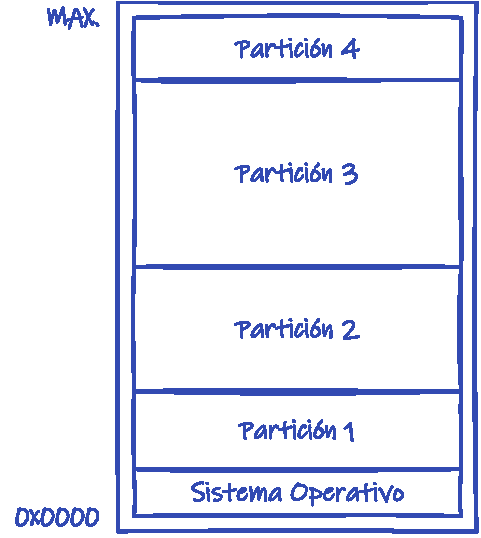
\includegraphics[width=0.8\textwidth]{media/C15_memoria_principal/particionado_fijo.pdf}
\caption{Particionado fijo de la memoria en el IBM OS/360.}
\end{figure}

Este método fue utilizado originalmente por el \{ibmos360\}, pero ya no
se utiliza

\subsection{Particionado dinámico}\label{_particionado_dinuxe1mico}

{} El \textbf{particionado dinámico} es una generalización del anterior:

\begin{enumerate}
\def\labelenumi{\arabic{enumi}.}
\item
  El sistema operativo mantiene una tabla indicando qué partes de la
  memoria están libres y cuáles ocupadas. Inicialmente toda la memoria
  está libre por lo que es considerada como un gran hueco de memoria
  disponible.
\item
  Cuando un proceso llega y necesita memoria, se le busca un hueco lo
  suficientemente grande para alojarlo. Si se encuentra, solo se le
  asigna el espacio necesario, que es marcado como ocupado. El resto
  sigue siendo un hueco libre, aunque de menor tamaño.
\item
  Si un proceso termina y se crean dos huecos adyacentes, se funden en
  uno solo.
\end{enumerate}

El \textbf{particionado dinámico} se utilizaba fundamentalmente en
\textbf{sistemas de procesamiento por lotes} y
\textbf{multiprogramados}. En este último caso, el sistema operativo
tenía una \textbf{cola de entrada} ordenada por el \textbf{planificador
de largo plazo} y la recorría asignando memoria a los procesos, hasta
que no quedara ningún hueco libre con tamaño suficiente para alojar al
siguiente en la cola. Entonces el sistema operativo podía esperar hasta
que algunos procesos terminarán y hubiera un hueco lo suficientemente
grande en la memoria, para el siguiente proceso, o podía seguir buscando
en la cola de entrada procesos de menores requerimientos, aunque para
ello tuviera que saltarse algunos procesos.

En general, en un momento dado el sistema operativo, debe satisfacer una
petición de tamaño \emph{N} con una lista de huecos libres de tamaño
variable. Esto no es más que un caso particular del problema clásico de
la asignación dinámica de almacenamiento, para el cual hay diversas
soluciones:

\begin{itemize}
\item
  En el \textbf{{}primer ajuste}{} se escoge el primer hueco lo
  suficientemente grande como para satisfacer la petición. La búsqueda
  puede ser desde el principio de la lista o desde donde ha terminado la
  búsqueda anterior.
\item
  En el \textbf{{}mejor ajuste}{} se escoge el hueco más pequeño que sea
  lo suficientemente grande para satisfacer la petición. Indudablemente
  esto obliga a recorrer la lista de huecos completa o a tenerla
  ordenada por tamaño.
\item
  En el \textbf{{}peor ajuste}{} se escoge el hueco más grande.
  Igualmente obliga a buscar en toda la lista de huecos o a tenerla
  ordenada por tamaño.
\end{itemize}

Para evaluar qué estrategia es la mejor, se han realizado algunas
simulaciones con los siguientes resultados:

\begin{itemize}
\item
  El \textbf{primer y el mejor ajuste} son mejores que el peor ajuste en
  términos de menor tiempo y mayor aprovechamiento del espacio de
  almacenamiento.
\item
  Si comparamos el \textbf{primer y el mejor ajuste} ninguno de ellos
  destaca sobre el otro en lo que a mejor aprovechamiento del espacio se
  refiere.
\item
  El \textbf{primer ajuste} es normalmente más rápido que el
  \textbf{mejor ajuste}.
\end{itemize}

\section{Fragmentación}\label{_fragmentaciuxf3n}

{} Las estrategias de asignación de espacio de almacenamiento
generalmente sufren de problemas de \textbf{fragmentación}. Vamos a
comentar brevemente cómo afecta la \textbf{fragmentación} a la
\textbf{asignación contigua de memoria}.

\subsection{Fragmentación externa}\label{_fragmentaciuxf3n_externa}

{} La \textbf{fragmentación externa} ocurre cuando hay suficiente
espacio libre para satisfacer una petición, pero el espacio no es
contiguo. Es decir, el espacio de almacenamiento está fraccionado en un
gran número de huecos de pequeño tamaño:

\begin{itemize}
\item
  Afecta tanto a la estrategia del \textbf{primer} como del
  \textbf{mejor ajuste}. Siendo el primero mejor en algunos sistemas y
  el segundo mejor en otros.
\item
  Algunos análisis estadísticos realizados con el \textbf{primer ajuste}
  revelan que incluso con algunas optimizaciones, con \emph{N} bloques
  asignados se pierden 0.5\emph{N} por \textbf{fragmentación externa}
  ---es decir, un tercio de toda la memoria no es utilizable---. A esto
  se lo conoce como la regla del 50\%.
\end{itemize}

Existen diversas soluciones a este problema:

\begin{itemize}
\item
  Utilizar técnicas de \textbf{{}compactación}, lo que consiste en mover
  los procesos para que toda la memoria libre quede en un único hueco de
  gran tamaño. Sin embargo, esto puede ser muy caro en términos de
  tiempo y solo puede ser realizado cuando la \textbf{asignación de
  direcciones absolutas se realiza en tiempo de ejecución}.
\item
  La otra solución es permitir que el \textbf{espacio de direcciones
  físico} de un proceso no sea contiguo. Es decir, que la memoria puede
  ser asignada a un proceso independientemente de donde esté disponible.
  Existen dos técnicas complementarias que utilizan esta solución: la
  paginación (véase el \hyperref[paginaciuxf3n]{???}) y la
  \href{https://es.wikipedia.org/wiki/Segmentaci\%C3\%B3n_de_memoria}{segmentación}.
\end{itemize}

\subsection{Fragmentación interna}\label{_fragmentaciuxf3n_interna}

{} La \textbf{fragmentación interna} se origina por la diferencia entre
el espacio solicitado y el espacio finalmente asignado.

Supongamos un hueco de espacio libre de 12987 bytes que se va a usar
para satisfacer una petición de 12985 bytes. Esto genera un hueco de 2
bytes, pero la cantidad de información que debemos guardar en la lista
de huecos para saber que dicho hueco está ahí, es mucho mayor que el
tamaño del hueco en sí mismo. Por lo tanto, no nos interesa tener huecos
de tamaño arbitrario.

La solución más común es dividir la memoria física en unidades de tamaño
fijo y asignarla en múltiplos del tamaño de dichos bloques. Esto hace
que, en general, se asigne más memoria de la que realmente se ha
solicitado y, por tanto, de la que realmente los procesos van a
utilizar. A esto se lo denomina \textbf{fragmentación interna}.

\section{Intercambio}\label{_intercambio}

{} {} Un proceso debe estar en la memoria para ser ejecutado, pero en
algunos sistemas operativos un proceso puede ser sacado de la memoria y
copiado a un almacenamiento de respaldo de forma temporal
---generalmente un dispositivo de almacenamiento secundario, como un
disco--- y en algún momento volver a ser traído a la memoria para
continuar su ejecución. Al procedimiento descrito se lo denomina
\textbf{intercambio} o \textbf{\emph{swapping}}.

\subsection{Implementación}\label{_implementaciuxf3n}

El \textbf{intercambio} se puede implementar de la siguiente manera:

\begin{enumerate}
\def\labelenumi{\arabic{enumi}.}
\item
  La \textbf{cola de preparados} contiene todos los procesos que esperan
  para ser ejecutados en la CPU.
\item
  Cuando el \textbf{planificador de la CPU} decide ejecutar un proceso,
  llama al \textbf{asignador}.
\item
  El \textbf{asignador} comprueba si el siguiente proceso que debe ser
  ejecutado está en la memoria. Si no lo está y no hay memoria libre, el
  \textbf{asignador} hace que el \textbf{gestor de la memoria}
  intercambie el proceso con alguno de los que sí lo está.
\item
  Finalmente, el \textbf{asignador} ejecuta el resto del cambio de
  contexto (véase el \hyperref[_cambio_de_contexto]{???}) para entregar
  la CPU al proceso seleccionado.
\end{enumerate}

Por ejemplo, si a un sistema con \textbf{planificación de CPU} basado en
prioridad llega a la \textbf{cola de preparados} un proceso de alta
prioridad, el \textbf{gestor de memoria} intercambia algunos procesos de
baja prioridad con el de alta prioridad y ejecuta este último. Cuando el
proceso de alta prioridad termina, los de baja prioridad pueden ser
intercambiados para continuar su ejecución.

\subsection{Limitaciones}\label{_limitaciones}

Sin embargo el \textbf{intercambio} presenta algunas limitaciones
importantes:

\begin{itemize}
\item
  Si un sistema \textbf{reubica las direcciones en tiempo de compilación
  o carga}, el proceso solo puede ser intercambiado en la misma región
  de la memoria. Sin embargo, si se utiliza \textbf{reubicación en
  tiempo de ejecución}, entonces el proceso puede ser intercambiado en
  cualquier región de la memoria, puesto que las \textbf{direcciones
  físicas} son calculadas durante la ejecución.
\item
  El \textbf{tiempo de cambio de contexto} en un sistema con
  \textbf{intercambio} puede ser mucho mayor, puesto que incluye el
  tiempo que se tarda en hacer el intercambio. La mayor parte del tiempo
  de intercambio es el tiempo de transferencia con el disco, que puede
  ser de varios cientos de milisegundos, incluso utilizando los discos
  más rápidos. Esto afecta al \textbf{tiempo de cuanto} que siempre debe
  ser mucho mayor que el tiempo de \textbf{cambio de contexto}.
\item
  Un proceso podría disponer de un espacio en memoria de 120 MiB pero
  estar utilizando solo 2 MiB. Por tanto, es interesante que el sistema
  operativo conozca con exactitud la memoria utilizada por el proceso
  ---y no la que podría estar utilizando como máximo--- para reducir el
  tiempo de transferencia de los datos al disco durante el intercambio.

  Para eso, el sistema operativo proporciona llamadas al sistema con las
  que un proceso con requerimientos dinámicos de memoria puede informar
  del cambio en su necesidad de memoria. Por ejemplo, los sistemas
  operativos modernos proporcionan llamadas al sistema para reservar y
  liberar memoria ---como \{clang\_malloc\} y \{clang\_free\} en los
  sistemas POSIX--- gracias a las que el sistema conoce las necesidades
  reales de los procesos.
\item
  El \textbf{intercambio} presenta dificultades cuando el proceso que va
  a ser sacado de la memoria está esperando por una operación de E/S que
  accede a la memoria del proceso para leer o escribir datos en ella.
  Las soluciones podrían ser:

  \begin{itemize}
  \item
    No intercambiar procesos con operaciones de E/S síncronas o
    asíncronas pendientes.
  \item
    Utilizar búferes del sistema operativo en las operaciones de E/S.
    Por ejemplo, en una operación \textbf{write} a un archivo, el
    sistema operativo copiaría primero los datos a un búfer interno y
    luego ordenaría la escritura de esos datos. Así el proceso podría
    ser intercambiado sin problemas. Las transferencias entre los
    búferes del sistema y la memoria de los procesos serían realizadas,
    por el sistema operativo, solo cuando los procesos residen en la
    memoria.
  \end{itemize}
\end{itemize}

Debido fundamentalmente a que el tiempo de intercambio es muy alto, no
se utiliza el intercambio estándar en los sistemas operativos actuales.
Lo que sí podemos encontrar en muchos sistemas son versiones modificadas
de este mecanismo.

Por ejemplo, en muchas versiones antiguas de UNIX y en los sistemas
modernos, el intercambio permanece desactivado y solo se activa cuando
la cantidad de memoria usada supera cierto límite. Además, en los
sistemas actuales no se intercambian procesos completos si no las
porciones menos usadas de cada proceso, como veremos en el
\hyperref[memoria_virtual]{???}.

\section{}

\textbf{Tiempo de lectura:} \{s16-reading-time\}

La traducción entre direcciones virtuales y físicas puede realizarse de
diversas maneras. La forma más extendida es la \textbf{{}paginación},
que no es sino un esquema de gestión de la memoria que permite que el
espacio de direcciones físico de un proceso no sea continuo, evitando el
problema de la \textbf{fragmentación externa}.

\section{Método básico}\label{_muxe9todo_buxe1sico}

En la paginación la memoria física se divide en bloques de tamaño fijo
denominados \textbf{marcos}{}, mientras que el espacio de direcciones
virtual se divide en bloques del mismo tamaño que los marcos,
denominados \textbf{páginas}{}. Cuando un proceso va a ser ejecutado,
sus páginas son cargadas desde el almacenamiento secundario en marcos
libres de la memoria física.

\begin{figure}
\centering
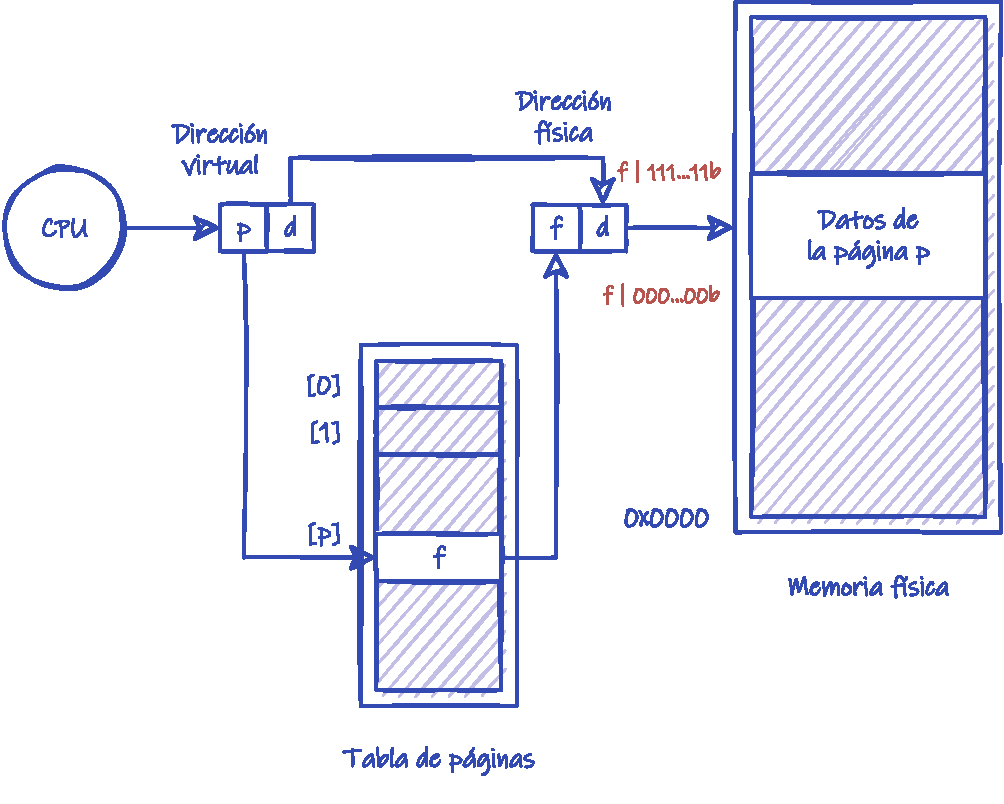
\includegraphics[width=0.8\textwidth]{media/C16_paginación/paginación.pdf}
\caption{Soporte del hardware para la
paginación.}\label{fig-paginaciuxf3n}
\end{figure}

La paginación es una forma de \textbf{reubicación de las direcciones en
tiempo de ejecución} donde la transformación de las direcciones
virtuales en direcciones físicas se realiza de la siguiente manera
(véase la \hyperref[fig-paginaciuxf3n]{Soporte del hardware para la
paginación.}):

\begin{enumerate}
\def\labelenumi{\arabic{enumi}.}
\item
  Cada dirección virtual generada por la CPU es divida en dos partes: un
  \textbf{número de página} \emph{p} y un \textbf{desplazamiento}
  \emph{d}.
\item
  El \textbf{número de página}{} es utilizado por la MMU para indexar la
  \textbf{tabla de páginas}{}, que contiene el \textbf{número de marco}
  \emph{f} de cada \textbf{página} en la memoria física.
\item
  El \textbf{número de marco}{} \emph{f} es combinado con el
  \textbf{desplazamiento} \emph{d} para generar la dirección física que
  va a ser enviada por el bus de direcciones hacia la memoria.
\end{enumerate}

El tamaño de las \textbf{páginas} ---y el de los \textbf{marcos}---
viene definido por el hardware y normalmente es un número entero
potencia de 2 que puede variar entre 512 bytes y 16 MiB, dependiendo de
la arquitectura. Es decir, si el espacio de direcciones es de
2\textsuperscript{\emph{m}} y el tamaño de página es de
2\textsuperscript{\emph{n}}, los \emph{m} - \emph{n} bits de mayor orden
de las direcciones virtuales indican el \textbf{número de página},
mientras que los \emph{n} bits de menor orden indican el
\textbf{desplazamiento} (véase la
\hyperref[fig-direcciuxf3n-virtual-paginaciuxf3n]{Descomposición de las
direcciones virtuales en paginación.}).

\begin{figure}
\centering
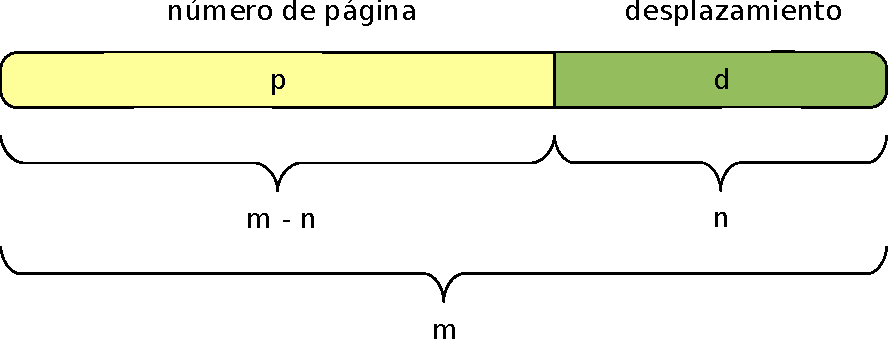
\includegraphics[width=0.8\textwidth]{media/C16_paginación/dirección_virtual_paginación.pdf}
\caption{Descomposición de las direcciones virtuales en
paginación.}\label{fig-direcciuxf3n-virtual-paginaciuxf3n}
\end{figure}

Por ejemplo, en muchos sistemas operativos el tamaño de página es de 4
KiB, por lo que el desplazamiento \emph{n} necesita:

\[n = log_2 4096 = 12\ "bits"\]

Si las direcciones virtuales son de 32 bits, eso deja para el número de
página \emph{p}:

\[p = 32 - 12 = 20\ "bits"\]

por lo que el espacio de direcciones virtual tiene 2\textsuperscript{20}
páginas ---es decir, 1 048 576 páginas---.

\subsection{Desde el punto de vista de los
procesos}\label{_desde_el_punto_de_vista_de_los_procesos}

Cada \textbf{página} de un proceso requiere un \textbf{marco}. Por
tanto, cuando un proceso llega al sistema:

\begin{enumerate}
\def\labelenumi{\arabic{enumi}.}
\item
  Si el proceso requiere \emph{n} \textbf{páginas}, el sistema operativo
  debe escoger \emph{n} \textbf{marcos}. Estos \textbf{marcos} son
  tomados de la \textbf{lista de marcos libres}{} que debe mantener el
  sistema. Puesto que son escogidos de allí donde los haya libres, el
  \textbf{espacio de direcciones físico} puede no ser contiguo, aunque
  los procesos vean un \textbf{espacio de direcciones virtual} contiguo.
\item
  Los \textbf{marcos} seleccionados son asignados al proceso y cada
  \textbf{página} del proceso es cargada en uno de dichos
  \textbf{marcos}.
\item
  La \textbf{tabla de páginas} es actualizada de manera que en la
  entrada de cada \textbf{página} del proceso se pone el número de
  \textbf{marco} correspondiente.
\end{enumerate}

Un aspecto importante de la paginación es la diferencia entre cómo ven
los procesos la memoria y como es realmente la memoria física. Cada
proceso ve la memoria como un espacio único que lo contiene solo a él.
Sin embargo, la realidad es que el programa está disperso por la memoria
física, que además puede almacenar a otros programas. Esto es posible
porque en cada momento la \textbf{tabla de páginas} solo contiene las
\textbf{páginas} del proceso en ejecución en la CPU.

\subsection{Desde el punto de vista del sistema
operativo}\label{_desde_el_punto_de_vista_del_sistema_operativo}

Puesto que el sistema operativo es quién gestiona la memoria física,
este debe saber:

\begin{itemize}
\item
  Que \textbf{marcos} están asignados y a que \textbf{página} de qué
  proceso o procesos.
\item
  Que \textbf{marcos} están disponibles.
\end{itemize}

Toda esta información generalmente se guarda en una estructura
denominada la \textbf{tabla de marcos}{}, que tiene una entrada por cada
\textbf{marco} de la memoria física.

Además, el sistema operativo debe mantener una copia de la \textbf{tabla
de páginas} para cada proceso en el \textbf{PCB}, igual que mantiene una
copia del contador de programa y del contenido de los registros de la
CPU. Esta copia es utilizada:

\begin{itemize}
\item
  Por el \textbf{asignador} para sustituir la \textbf{tabla de páginas}
  usada por la CPU cuando realiza un \textbf{cambio de contexto}. Por lo
  tanto, el uso de la paginación incrementa el tiempo del cambio de
  contexto.
\item
  Para la traducción manual de direcciones virtuales en físicas. Por
  ejemplo, cuando un proceso realiza una llamada al sistema para
  realizar una operación de E/S y proporciona una dirección como
  parámetro, dicha dirección debe ser traducida manualmente para
  producir la dirección física correspondiente, que será comunicada al
  hardware para realizar la operación.
\end{itemize}

\subsection{Tamaño de las páginas}\label{_tamauxf1o_de_las_puxe1ginas}

Una decisión de diseño importante es escoger el tamaño de las
\textbf{páginas} adecuado:

\begin{itemize}
\item
  Con \textbf{páginas} más pequeñas esperamos tener menos
  \textbf{fragmentación interna}.
\item
  Con páginas más grandes se pierde menos espacio en la \textbf{tabla de
  páginas}. No olvidemos que cuanto más pequeñas son las
  \textbf{páginas}, más \textbf{páginas} son necesarias y, por tanto,
  más entradas en la \textbf{tabla de páginas} se necesitan. Además, la
  E/S es más eficiente cuanto más datos son transferidos de cada vez.
\end{itemize}

Los tamaños de \textbf{páginas} típicos son 4 y 8 KiB. En un sistema de
32 bits con páginas de 4 KiB ---como del que hablamos antes--- el
espacio de direcciones virtual tiene 1 048 576 páginas. Si se utilizan 4
bytes para cada entrada de la \textbf{tabla de páginas} ---aunque esto
también puede variar--- eso significa que cada \textbf{tabla de páginas}
ocupa 4 MiB de espacio. Mientras que con \textbf{páginas} de 8 KiB, la
\textbf{tabla de páginas} ocuparía 2 MiB de espacios.

También significa que si los 4 bytes de la \textbf{tabla de páginas} se
utilizan para guardar únicamente el \textbf{número de marco}, cada
entrada puede direccionar a uno de 2\textsuperscript{32} ---o 4 GiB---
\textbf{marcos} de la memoria física. Si el tamaño de cada
\textbf{marco} es de 4 KiB ---dado que debe coincidir con el tamaño de
las páginas--- podemos determinar que el sistema es capaz de direccionar
2\textsuperscript{44} bytes ---o 16 TiB--- de memoria física, aunque el
espacio de direcciones virtual de cada proceso solo le da acceso a un
máximo de 4 GiB.

\section{Soporte hardware de la tabla de
páginas}\label{_soporte_hardware_de_la_tabla_de_puxe1ginas}

La implementación en hardware de la \textbf{tabla de páginas} puede
realizarse de diversas maneras.

\subsection{Almacenada en registros de la
CPU}\label{_almacenada_en_registros_de_la_cpu}

La \textbf{tabla de páginas} del proceso actual en la CPU puede alojarse
dentro de la propia CPU, en unos registros destinados a tal fin.

Debido a la velocidad de los registros de la CPU, la implementación en
registros es la más eficiente. Sin embargo, solo puede ser utilizado
para \textbf{tablas de páginas} razonablemente pequeñas, ya que alojar
tablas de más de 256 entradas en registros es muy costoso.

Por ejemplo, el DEC \href{https://es.wikipedia.org/wiki/PDP-11}{PDP-11}
---para el que se diseñó el primer UNIX--- es un ejemplo de sistema con
esta implementación. Utilizaba un espacio de direcciones de 16 bits y un
tamaño de \textbf{páginas} de 8 KiB, por lo que solo necesitaba 8
registros dedicados para alojar toda la \textbf{tabla de páginas}.

\subsection{Almacenada en memoria}\label{_almacenada_en_memoria}

La otra opción es alojar la \textbf{tabla de páginas} del proceso actual
en la memoria, normalmente en un formato definido por la CPU.

En los sistemas modernos se utilizan \textbf{tablas de páginas} de un
millón de entradas o más, que difícilmente pueden alojarse en registros
dentro de la CPU. Por eso, los sistemas actuales almacenan la
\textbf{tabla de páginas} del proceso actualmente en ejecución, en la
memoria. Eso permite disponer de \textbf{tablas de páginas} de gran
tamaño, aunque a costa de necesitar dos accesos a la memoria física por
cada acceso a una dirección virtual.

Para que la MMU pueda conocer la ubicación de la \textbf{tabla de
páginas} durante la traducción de las direcciones, la CPU debe disponer
de un registro ---el \textbf{{}PTBR} (\emph{Page-Table Base
Register})--- donde se guarda la dirección de la \textbf{tabla de
páginas} actual.

Además, esto tiene la ventaja de que el \textbf{cambio de contexto} es
más rápido ---respecto al uso de registros para almacenar la tabla de
páginas--- puesto que solo es necesario cargar un único registro más
---el \textbf{PTBR}--- durante el mismo.

\subsection{TLB}\label{_tlb}

La solución al retraso originado por el acceso a la tabla de páginas,
cuando esta está en la memoria, pasa porque el sistema disponga de una
pequeña caché de traducciones en hardware llamada \textbf{{}TLB}
(\emph{Translation Look-aside Buffer}).

La \textbf{TLB} es una memoria asociativa de alta velocidad. Cada
entrada de la \textbf{TLB} tiene dos partes: la \textbf{clave} ---o
etiqueta--- y el valor. Cuando a la \textbf{TLB} se le entrega un
elemento, este es comparado simultáneamente con todas las claves. Si se
produce alguna coincidencia, la memoria devuelve el valor de la entrada
correspondiente.

Debido a la forma que tienen de operar, son rápidas pero muy caras de
fabricar. Por ello, el número de entradas es bajo, normalmente entre 64
y 1024.

\subsubsection{Uso básico de la TLB}\label{_uso_buxe1sico_de_la_tlb}

La \textbf{TLB} es utiliza con la \textbf{tabla de páginas} de la
siguiente manera:

\begin{figure}
\centering
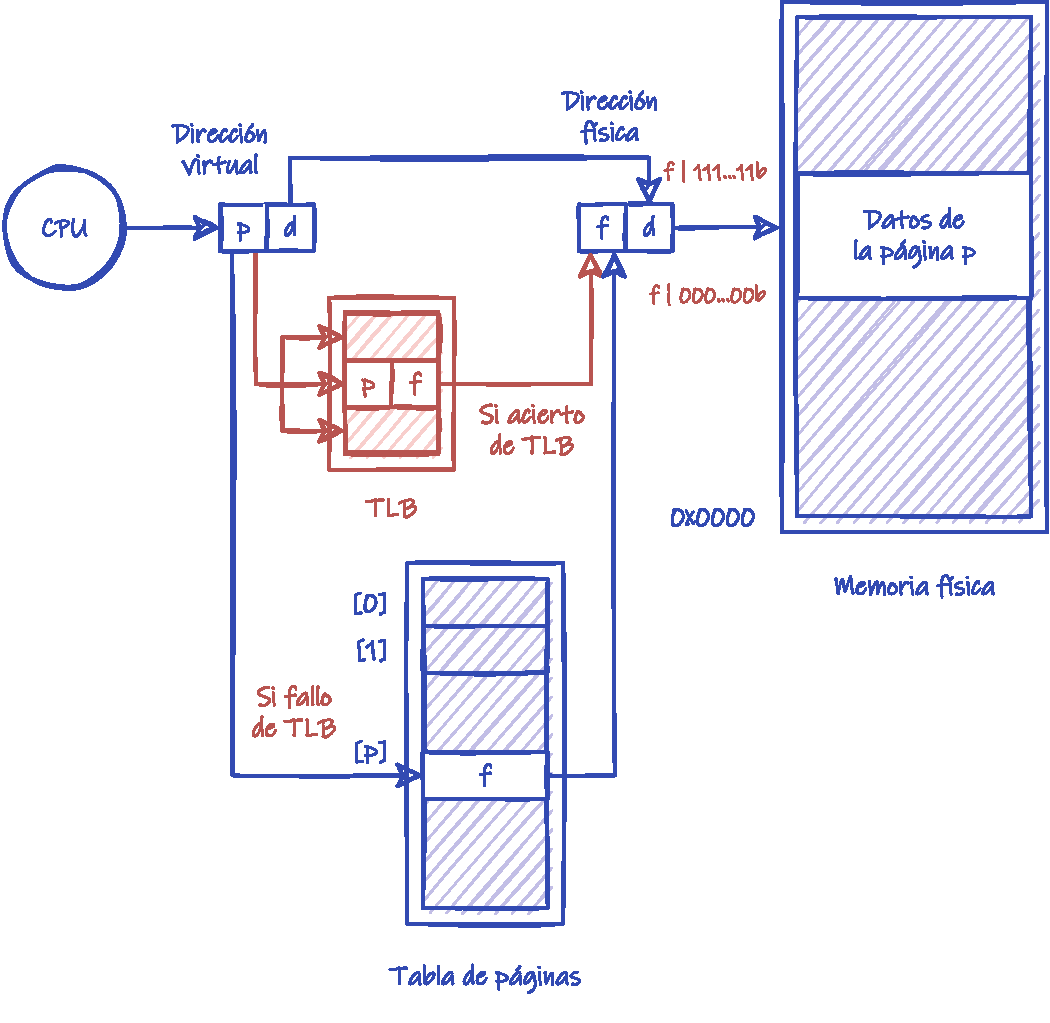
\includegraphics[width=0.8\textwidth]{media/C16_paginación/tlb.pdf}
\caption{Soporte del hardware para la paginación con
TLB.}\label{fig-paginaciuxf3n-tlb}
\end{figure}

\begin{enumerate}
\def\labelenumi{\arabic{enumi}.}
\item
  La \textbf{TLB} contiene unas pocas entradas de la \textbf{tabla de
  páginas}.
\item
  Cuando la CPU genera una dirección virtual, el \textbf{número de
  página} es entregado a la \textbf{TLB}. La \textbf{TLB} utiliza los
  números de páginas como \textbf{clave}, por lo que si hay alguna
  coincidencia, devolverá la entrada correspondiente de la \textbf{tabla
  de páginas}.
\item
  Si hay coincidencia ---o \textbf{acierto de TLB}--- el \textbf{número
  de marco} es extraído de la entrada devuelta por la \textbf{TLB} y es
  utilizado para generar la dirección física. Todo este proceso puede
  requerir un 10\% más de tiempo que si no se hiciera la traducción de
  las direcciones.
\item
  Si no hay coincidencia ---o \textbf{fallo de TLB}--- es necesario
  acceder a la \textbf{tabla de páginas} para obtener la entrada
  correspondiente directamente de ella. Indudablemente, este acceso
  puede beneficiarse de la existencia de diferentes niveles de caché en
  el acceso a la memoria principal.
\item
  En este último caso, la entrada recuperada debe ser añadida a la
  \textbf{TLB}, por lo que sí está llena, se debe seleccionar una para
  ser sustituida. Los algoritmos de reemplazo utilizados van, desde
  elegir una aleatoriamente, hasta el \textbf{{}LRU} (\emph{Least
  Recently Used}).
\end{enumerate}

\subsubsection{Borrado de la TLB en el cambio de
contexto}\label{_borrado_de_la_tlb_en_el_cambio_de_contexto}

Una cuestión importante es qué ocurre con las \textbf{TLB} cuando el
sistema operativo realiza un \textbf{cambio de contexto}.

En general, es necesario que el asignador realice un borrado de la
\textbf{TLB}. De lo contrario, el nuevo proceso podría utilizar las
entradas de la \textbf{tabla de páginas} del viejo proceso, que
estuvieran almacenadas en la \textbf{TLB}. Sin embargo, un proceso no
tiene por qué utilizar todas las entradas de la \textbf{TLB}, por lo que
sería más interesante, no tener que borrar las entradas de procesos
anteriores, mientras no sean necesarias, por si estos vuelven a ser
ejecutados en la CPU.

El borrado se puede evitar si cada entrada de la \textbf{TLB} tiene un
\textbf{{}ASID} (\emph{Address-Space Identification}), que no es más que
un identificador único para cada proceso. En este tipo de \textbf{TLB},
en la \textbf{clave} se buscan pares \textbf{(número de página, ASID)},
donde el primero proviene de la dirección virtual y el segundo es el
\textbf{ASID} del proceso actual. De esta forma, si el \textbf{número de
página} coincide, pero no el \textbf{ASID}, se produce un fallo de la
\textbf{TLB}. Esto obliga a acceder a la \textbf{tabla de páginas} en
memoria para recuperar la entrada, evitando que se lea por error la
entrada de un proceso anterior.

Esta característica está presente en los procesadores \{decalpha\},
\{mips\} y \{ultrasparc\}. Entre 2005 y 2006 también comenzó a ser
incluida en algunos procesadores de la familia x86, a través de las
extensiones de virtualización Intel VT y AMD Pacifica.

\section{Tiempos de acceso a la
memoria}\label{_tiempos_de_acceso_a_la_memoria}

El rendimiento de un sistema con paginación, está relacionado con el
concepto de \textbf{tiempo de acceso efectivo}{} a la memoria
\(T_text(em)\), que intenta estimar el tiempo que realmente se tarda en
acceder a la memoria, teniendo en cuenta mecanismos del sistema
operativo como el método de paginación o la existencia de \textbf{TLB}.

En muchos sistemas informáticos, el \textbf{tiempo de acceso}{} a la
memoria física \(T_text(m)\) es de unos pocos nanosegundos. Por tanto,
en el método de básico de paginación ---con una \textbf{tabla de páginas
lineal}{}--- y sin \textbf{TLB}, el \textbf{tiempo de acceso efectivo}
\(T_text(em)\) es el doble del \textbf{tiempo de acceso} \(T_text(m)\) a
la memoria:

\[T_text(em)=2T_text(m)\]

porque es necesario acceder a la memoria en dos ocasiones:

\begin{enumerate}
\def\labelenumi{\arabic{enumi}.}
\item
  Primero, para consultar la \textbf{tabla de páginas}, con el objetivo
  de traducir la dirección virtual en una dirección física.
\item
  Después, para realizar la operación solicitada sobre la memoria
  física.
\end{enumerate}

Obviamente, en métodos de paginación donde hagan falta más accesos para
obtener finalmente el \textbf{número de marco}, el \textbf{tiempo de
acceso efectivo} será mayor.

En el caso anterior, el segundo acceso a la memoria es inevitable,
porque corresponde a la operación solicitada por el proceso. Mientras
que el primero puede evitarse, en ciertas ocasiones, consultado la
\textbf{TLB} antes de acceder a la \textbf{tabla de páginas}. Es decir,
en un sistema con \textbf{TLB}:

\begin{itemize}
\item
  Cuando la dirección virtual \textbf{NO} está en la \textbf{TLB}:
  \(T_text(em)=2T_text(m) + T_text(TLB)\), porque primero se accede a la
  \textbf{TLB} y después ---como no se encuentra allí la direcció
  virtual--- se consulta la \textbf{tabla de páginas}.
\item
  Cuando la dirección virtual está en la \textbf{TLB}:
  \(T_text(em)=T_text(m) + T_text(TLB)\), porque la \textbf{TLB}
  proporciona la información necesaria para traducir la dirección,
  evitando la consulta posterior a la \textbf{tabla de páginas}.
\end{itemize}

El cálculo de \(T_text(em)\) puede complicarse aun más si tenemos en
cuenta que los sistemas suelen tener varios niveles de memoria caché. En
ese caso \(T_text(m)\) no tiene un valor determinado, sino que se estima
un promedio considernado tanto el tiempo de acceso a la memoria física
como a cada uno de los niveles de caché del sistema, así como la
probabilidad de que la dirección de memoria a la que se quiere acceder
esté disponible en alguno de dichos niveles.

El \(T_text(em)\) del primer caso suele ser mucho mayor que el segundo
porque, por lo general, \(T_text(TLB) ll T_text(m)\). Esto hace que en
muchos sistemas se pueda considerar que \(T_text(em) ~~ T_text(m)\)
cuando la dirección virtual está en la \textbf{TLB}.

Como el \textbf{tiempo de acceso efectivo} \(T_text(em)\) ahora depende
de la probabilidad \(p_text(TLB)\) de que las direcciones virtuales
consultadas estén en la \textbf{TLB}, ya no podemos hacer el cálculo de
forma determinista, sino estimar un \(T_text(em)\) promedio para el
sistema. Para ello, solo es necesario sumar el \(T_text(em)\) para ambos
casos, ponderando por la probabilidad \(p_text(TLB)\) de que la
dirección esté en la \textbf{TLB} o \((1 - p_text(TLB))\) de que no esté
en la \textbf{TLB}, respectivamente:

\[{:(T_"em", =, (1-p_"TLB")*(2T_"m" + T_"TLB") + p_"TLB"*(T_"m" + T_"TLB")),
    (    , =, (2-p_"TLB")*T_"m" + T_"TLB"\qquad\qquad\qquad\qquad\qquad\ \ \ ):}\]

Como comentamos anteriormente, esta expresión se puede simplificar si
consideramos que \(T_text(TLB) ll T_text(m)\):

\[{:(T_"em", =, 2*(1-p_"TLB")*T_"m" + p_"TLB"*T_"m"),
    (    , =, (2-p_"TLB")*T_"m"\qquad\qquad\qquad\ \ \ ):}\]

Obviamente, cuanto más se aproxima a 1 la probabilidad \(p_text(TLB)\)
de que la entrada esté en la \textbf{TLB}, más cerca está \(T_text(em)\)
de \(T_text(m)\).

Para mejorar esta probabilidad:

\begin{itemize}
\item
  Las \textbf{TLB} permiten marcar algunas entradas como insustituibles.
  Esto normalmente se hace con las entradas de las \textbf{páginas} del
  código y los datos del núcleo, ya que son páginas que se utilizan con
  muchísima frecuencia.
\item
  Si la MMU soporta páginas de mayor tamaño que el estándar, se utilizan
  para alojar el código y los datos del núcleo. De esta forma se
  minimiza el número de entradas de la \textbf{TLB} que utilizan, con el
  fin de disponer de más entradas libres para los procesos en ejecución.
\end{itemize}

En la familia x86 el tamaño de página estándar es de 4 KiB, pero también
se puede disponer de páginas de 4 MiB. En x86-64 las páginas de gran
tamaño son de 2 MiB, aunque algunos modelos también soportan páginas de
1 GiB.

\section{Protección de la memoria}\label{_protecciuxf3n_de_la_memoria}

La protección de las páginas se consigue mediante unos bits que indican
las operaciones que se pueden realizar sobre ellas. Normalmente, estos
bits son almacenados en cada una de las entradas de la \textbf{tabla de
páginas}.

\subsection{Bits de protección}\label{_bits_de_protecciuxf3n}

{} Los \textbf{bits de protección} pueden ser:

\begin{itemize}
\item
  \textbf{Solo lectura}.
\item
  \textbf{Lectura --- Escritura}. En algunos sistemas hay un bit
  específico para este permiso, mientras que en otros se utilizan bits
  separados, como: \textbf{lectura}, \textbf{escritura} y
  \textbf{ejecución}; que se pueden combinar libremente.
\item
  \textbf{Solo ejecución}. Que no existen en todas las plataformas. Por
  ejemplo, la familia x86 careció de esta característica hasta que AMD
  la incluyó en su arquitectura x86-64, lo que obligó a Intel a
  incluirla en las versiones más modernas de Pentium IV. El bit ---que
  para ser exacto indica \textbf{no ejecución}--- fue introducido para
  evitar cierto tipo de ataques de seguridad.
\end{itemize}

Durante la traducción de las direcciones, la MMU comprueba que el tipo
de acceso sea válido. Si no lo es, se genera una excepción de violación
de protección de memoria, dado que el acceso en un modo no autorizado se
considera una instrucción privilegiada. Normalmente, el sistema
operativo responde a dicha excepción terminando el proceso que la
generó.

\subsection{Bit de válido}\label{_bit_de_vuxe1lido}

{} Además de los \textbf{bits de protección} comentados, se suele añadir
a cada entrada un \textbf{bit de válido}:

\begin{itemize}
\item
  Cuando una \textbf{página es válida}, la página existe en el espacio
  de direcciones virtual del proceso. Es decir, que la página se puede
  utilizar. Otro término comúnmente utilizado, es que la página es
  \textbf{legal}{}.
\item
  Cuando la \textbf{página es inválida}, la página no existe en el
  espacio de direcciones virtual del proceso. Es decir, que la página no
  se puede utilizar. El término alternativo utilizado es que la página
  es \textbf{ilegal}{}.
\end{itemize}

Al igual que con los \textbf{bits de protección}, los intentos de acceso
a una página ilegal generan una excepción.

El sistema operativo puede utilizar este bit para permitir o denegar
cualquier tipo de acceso a una \textbf{página}. Generalmente, porque no
se le ha asignado un \textbf{marco} de memoria física, ya que esa página
no está siendo utilizada por el proceso.

\begin{figure}
\centering
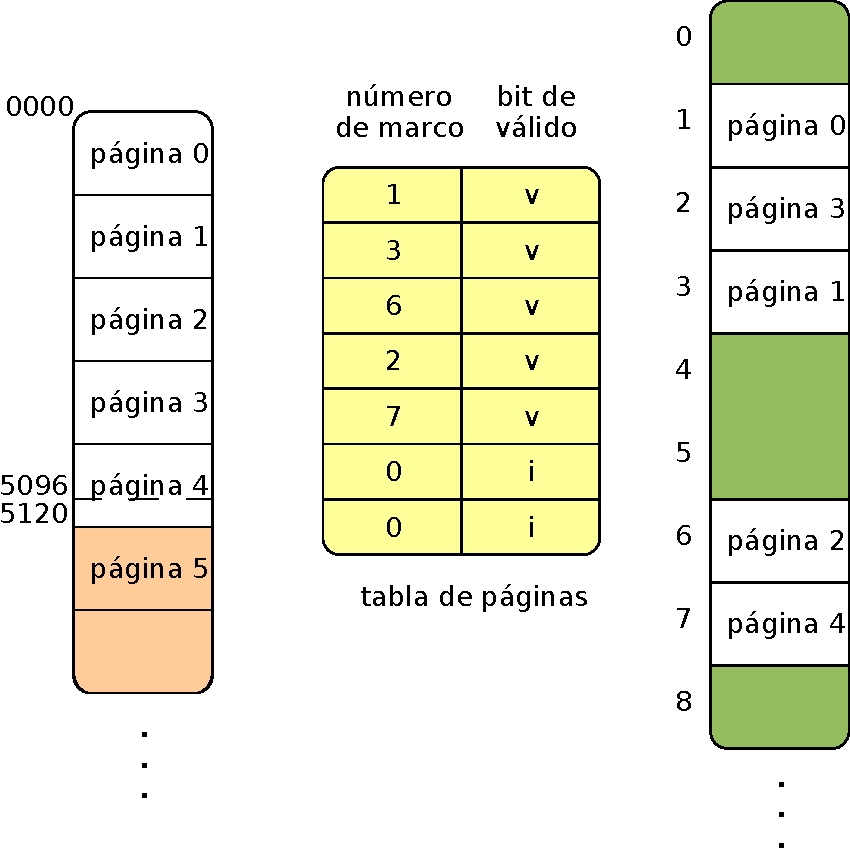
\includegraphics[width=0.8\textwidth]{media/C16_paginación/bit_de_válido_en_la_tabla_de_páginas.pdf}
\caption{Bit de válido en la tabla de
páginas.}\label{fig-bit-de-vuxe1lido-en-la-tabla-de-puxe1ginas}
\end{figure}

Por ejemplo, en la
\hyperref[fig-bit-de-vuxe1lido-en-la-tabla-de-puxe1ginas]{Bit de válido
en la tabla de páginas.}, vemos el espacio de direcciones virtual y la
\textbf{tabla de páginas} de un proceso de 5096 bytes en un sistema con
\textbf{páginas} de 1 KiB. Puesto que el proceso no ocupa todo el
espacio de direcciones, solo las direcciones de la 0 a la 5119 son
válidas. En dicho ejemplo, podemos apreciar varios fenómenos:

\begin{itemize}
\item
  Debido a la \textbf{fragmentación interna}, las direcciones de la 5097
  a la 5119 son válidas, aunque el proceso solo ocupe hasta la 5096. Es
  decir, se está asignando al proceso una porción de memoria que no
  necesita.
\item
  Solo las \textbf{páginas} con datos y código del proceso son válidas.
  Mientras que todas las \textbf{páginas} con direcciones por encima de
  la 5119 están marcadas como ilegales.
\end{itemize}

En general, los procesos solo necesitan una porción muy pequeña de su
espacio de direcciones virtual. Por ejemplo, en un sistema de 32 bits,
muy pocos procesos necesitan los 3 GiB disponibles como máximo para cada
proceso ---el 1 GiB restante suele estar ocupado por el núcleo del
sistema---. Utilizando el \textbf{bit de válido}, el sistema operativo
no tiene que asignar \textbf{marcos} a \textbf{páginas} no utilizadas
por el proceso, ahorrando mucha memoria.

En el \hyperref[_tamauxf1o_de_las_puxe1ginas]{Tamaño de las páginas},
vimos que el tamaño de la \textbf{tabla de páginas} se puede calcular
como el número máximo de páginas del espacio de direcciones virtual
multiplicado por el tamaño de cada entrada de la tabla. Así, en un
sistema de 32 bits con páginas de 4 KiB y 4 bytes por entrada, se
necesitan 4 MiB de memoria para almacenar la \textbf{tabla de páginas}.
Como un proceso suele ocupar muy poco de su espacio de direcciones
virtual, suele ser un desperdicio de memoria crear y almacenar una
\textbf{tabla de páginas} completa, con una entrada para cada
\textbf{página} del espacio de direcciones.

Para evitarlo, en algunas CPU existe el registro \textbf{{}PTLR}
(\emph{Page-Table Length Register}) que se utiliza para indicar el
tamaño actual de la \textbf{tabla de páginas}. Este valor es comparado
por la MMU, durante la traducción de las direcciones virtuales, con el
\textbf{número de página} de cada dirección virtual, de manera que las
\textbf{páginas} con entradas más allá de la última almacenada en la
tabla son consideradas ilegales.

\begin{figure}
\centering
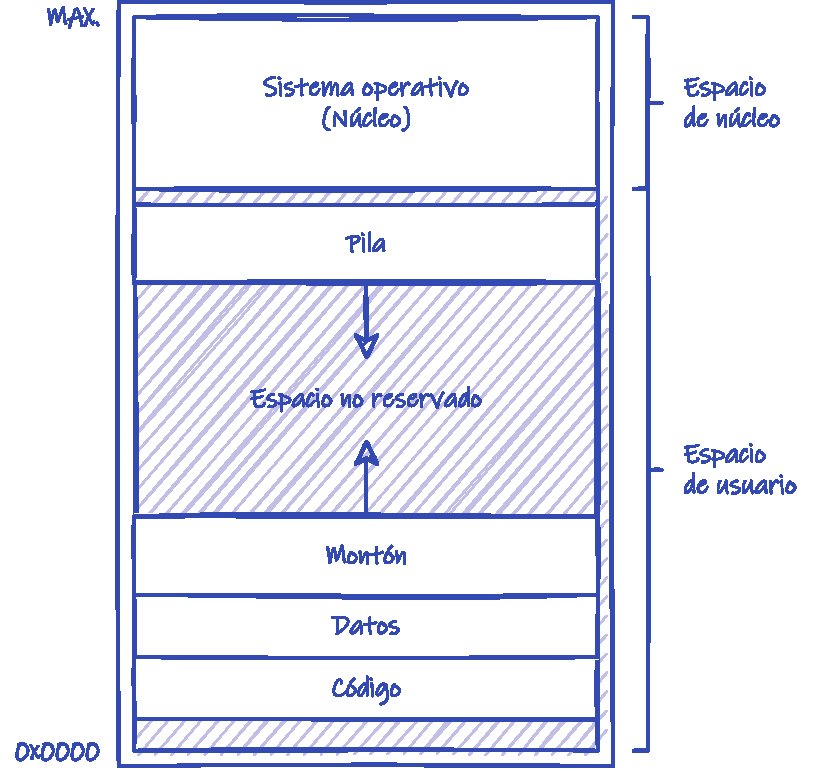
\includegraphics[width=0.8\textwidth]{media/C16_paginación/proceso_en_memoria.pdf}
\caption{Anatomía de un proceso en
memoria.}\label{fig-proceso-en-memoria-disperso}
\end{figure}

En realidad, el registro \textbf{PTLR} no es de mucha utilidad en los
sistemas operativos modernos porque, tal y como vimos en el
\hyperref[_el_proceso]{???}, lo más común es que los procesos tengan un
espacio de direcciones virtual disperso como el de la
\hyperref[fig-proceso-en-memoria-disperso]{Anatomía de un proceso en
memoria.}. En ella, podemos observar, como el sistema operativo ubica
los diferentes componentes del proceso de una forma particular dentro
del espacio de direcciones virtual. Este esquema permite que tanto el
\textbf{montón} ---a través del mecanismo de asignación dinámica de
memoria--- como la \textbf{pila} puedan extenderse ---según las
necesidades de memoria que tenga el proceso--- sobre la región de
memoria no ocupada. Esa región también puede ser parcialmente ocupada
por \textbf{librerías de enlace dinámico} o regiones de \textbf{memoria
compartida}, si son necesarias durante la ejecución del proceso.

En cualquier caso, las \textbf{páginas} de la región no ocupada, forman
parte del espacio de direcciones virtual, pero no necesitan tener
asignado ningún \textbf{marco} de memoria física, en tanto en cuanto el
proceso no las vaya a utilizar. La falta de \textbf{marco} es indicada
por el sistema operativo utilizando el \textbf{bit de válido} para
denegar el acceso.

\section{Páginas compartidas}\label{_puxe1ginas_compartidas}

{} Una de las ventajas importantes de la paginación, es la posibilidad
de compartir \textbf{páginas} entre procesos. Para conseguir esto, basta
con que las \textbf{páginas compartidas} de los distintos procesos
tengan asignadas un mismo \textbf{marco}. Esto permite, por ejemplo, que
los procesos de un mismo programa puedan compartir las \textbf{páginas}
de código o los datos de solo lectura con el fin de ahorrar memoria.
También permite compartir las \textbf{páginas} de código de una librería
compartida enlazada en diferentes procesos.

Compartir \textbf{páginas} no solo permite ahorrar memoria, pues en los
sistemas operativos modernos, la comunicación entre procesos mediante
memoria compartida (véase el \hyperref[memoria_compartida]{???}), se
implementa mediante \textbf{páginas compartidas}.

\section{Paginación jerárquica}\label{_paginaciuxf3n_jeruxe1rquica}

{} Al método básico de paginación, se lo conoce como \textbf{tabla de
páginas lineal}{}. Sin embargo, las CPU comúnmente, utilizan otras
técnicas a la hora de estructurar la \textbf{tabla de páginas}. Una de
las más comunes es la \textbf{paginación jerárquica}, utilizada en los
procesadores de la familia x86 y en ARM, entre otros.

La mayor parte de los sistemas modernos soportan el uso de espacios de
direcciones de gran tamaño. Por ejemplo, supongamos un sistema con un
espacio de direcciones virtual de 32 bits:

\begin{longtable}[]{@{}
  >{\raggedright\arraybackslash}p{(\linewidth - 2\tabcolsep) * \real{0.5000}}
  >{\raggedright\arraybackslash}p{(\linewidth - 2\tabcolsep) * \real{0.5000}}@{}}
\toprule\noalign{}
\endhead
\bottomrule\noalign{}
\endlastfoot
\textbf{tamaño del espacio de direcciones} & = 2\textsuperscript{32} = 4
GiB \\
\textbf{tamaño de página} & = 2\textsuperscript{12} = 4 KiB \\
\textbf{número de páginas} & = 2\textsuperscript{32} /
2\textsuperscript{12} = 2\textsuperscript{32-12} = 2\textsuperscript{20}
= 1 048 576 entradas \\
\end{longtable}

Es decir, que si el tamaño de cada entrada fuera de 4 bytes, la
\textbf{tabla de páginas} de un proceso podría ocupar hasta 4 MiB; que
debe ser alojada en una región continúa del espacio de direcciones
físico, por lo que podría darse el caso de que en algún momento no
hubiera un hueco contiguo lo suficientemente grande. Una forma de
resolver este problema es partir la \textbf{tabla de páginas}, de manera
que no sea necesario asignarle memoria de forma contigua.

\subsection{Paginación jerárquica de dos
niveles}\label{_paginaciuxf3n_jeruxe1rquica_de_dos_niveles}

La \textbf{paginación jerárquica} se basa en la idea de que un vector de
gran tamaño puede ser mapeado en uno más pequeño, que a su vez, puede
ser mapeado en un vector de menor tamaño.

\begin{figure}
\centering
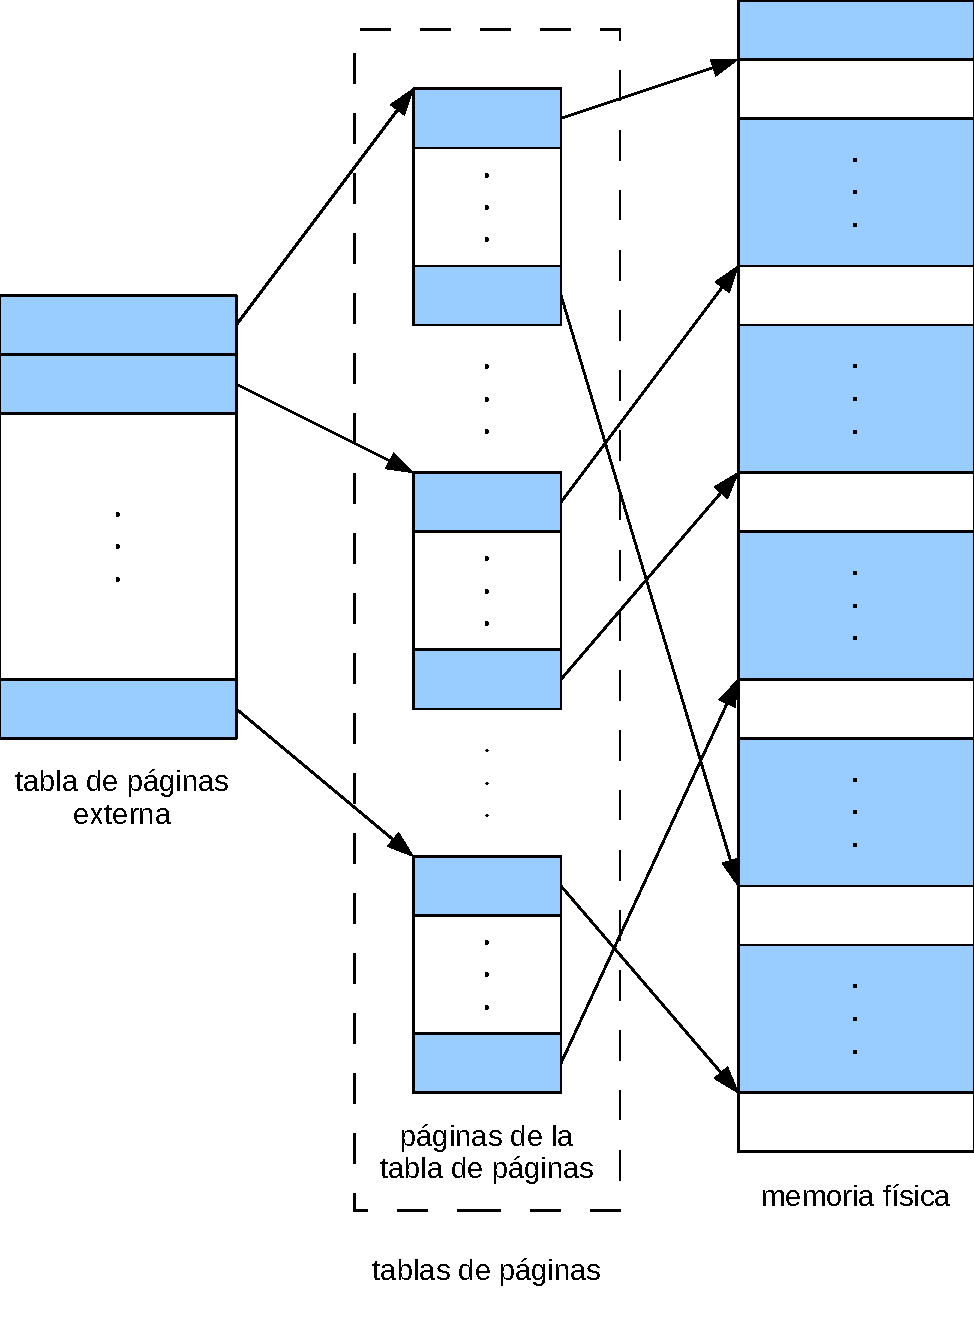
\includegraphics[width=0.8\textwidth]{media/C16_paginación/paginación_jerárquica.pdf}
\caption{Esquema de paginación jerárquica de dos
niveles.}\label{fig-paginaciuxf3n-jeruxe1rquica}
\end{figure}

Por ejemplo, si asumimos el caso anterior de un sistema con un espacio
de direcciones de 32 bits y un tamaño de página de 4 KiB, entonces
podemos dividir la tabla de páginas de 1 048 576 entradas ---4 MiB si
cada entrada necesita 4 bytes--- en 1024 porciones, cada una de las
cuales cabría en un \textbf{marco} de 4 KiB.

Estos \textbf{marcos}, a su vez, pueden ser mapeados por 1024 entradas
con las direcciones físicas de cada \textbf{marco}. Si organizamos estas
1024 entradas en un vector lineal, obtendremos una \textbf{tabla de
páginas externa}{} de 4 KiB (véase la
\hyperref[fig-paginaciuxf3n-jeruxe1rquica]{Esquema de paginación
jerárquica de dos niveles.}).

Dado que 4 KiB es una cantidad de memoria muy pequeña, muchos sistemas
operativos mantienen la \textbf{tabla de páginas externa} en la memoria
mientras el proceso se está ejecutando. Sin embargo, ahora la
\textbf{tabla de páginas} está dividida en \textbf{marcos}, que no
tienen por qué ser asignados de forma contigua en la memoria. Incluso
podrían ser intercambiados al disco, en caso de necesitar memoria libre.

Para tener dos niveles de 1024 entradas, solo es necesario dividir el
\textbf{número de página} \emph{p} de la dirección virtual ---que tenía
2\textsuperscript{20} bits--- en dos \textbf{números de página} de
2\textsuperscript{10} bits cada uno:

\begin{figure}
\centering
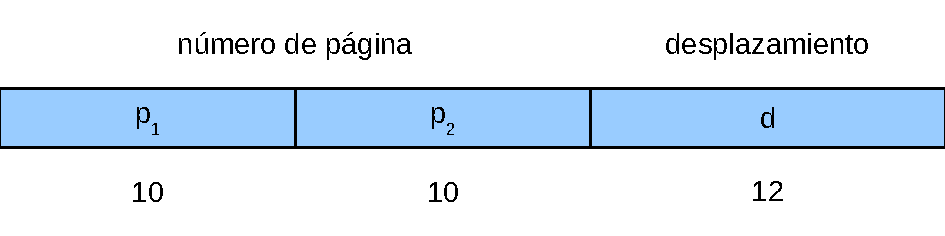
\includegraphics[width=0.8\textwidth]{media/C16_paginación/dirección_virtual_paginación_jerárquica.pdf}
\caption{}
\end{figure}

Este es el método utilizado por la familia de procesadores x86.

Otra variación de la \textbf{paginación jerárquica de dos niveles} es la
utilizada por VAX. Estos sistemas utilizaban una arquitectura de 32 bits
con un tamaño de página de 512 bytes. Las direcciones virtuales eran
divididas de la siguiente manera:

\begin{figure}
\centering
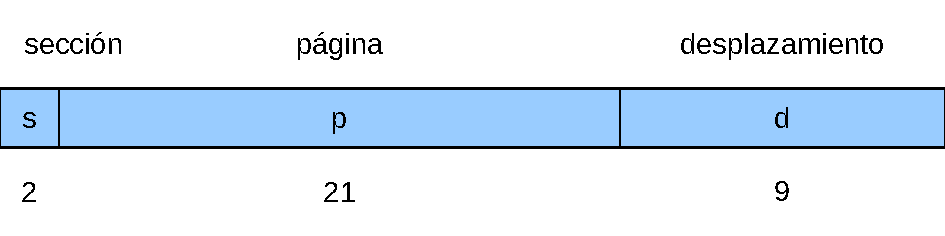
\includegraphics[width=0.8\textwidth]{media/C16_paginación/dirección_virtual_vax.pdf}
\caption{}
\end{figure}

El espacio de direcciones de un proceso estaba dividido en 3 secciones.
Los 2 bits de orden más alto \emph{s} de las direcciones virtuales se
utilizaban para indicar la \textbf{sección}. Cada \textbf{sección}
estaba dividida en \textbf{páginas} de 512 bytes, por lo que los
siguientes 21 bits de las direcciones virtuales \emph{p} eran utilizadas
para seleccionar la \textbf{página} concreta.

Dividiendo el espacio de direcciones de esta manera, el sistema
operativo podía mantener secciones sin utilizar mientras no fueran
necesarias. Esto era importante, puesto que la \textbf{tabla de páginas}
de una \textbf{sección} tenía un tamaño de 8 MiB.

\subsection{Paginación jerárquica de N
niveles}\label{_paginaciuxf3n_jeruxe1rquica_de_n_niveles}

En general, en la \textbf{paginación jerárquica} de \emph{n} niveles el
\textbf{número de página} \emph{p} de cada dirección virtual es dividido
en \emph{n} números: \{ \emph{p}\textsubscript{1},
\emph{p}\textsubscript{2}, \emph{p}\textsubscript{3}, \ldots,
\emph{p\textsubscript{N}}\}, donde:

\begin{enumerate}
\def\labelenumi{\arabic{enumi}.}
\item
  \emph{p}\textsubscript{1} se utiliza para indexar la \textbf{tabla de
  páginas externa} ---también llamada \textbf{directorio de páginas}{} o
  \textbf{tabla de páginas de nivel 0}{}--- cuya dirección conoce la CPU
  mediante el \textbf{PTBR}. La entrada obtenida de esta manera,
  contiene la dirección en la memoria física de una porción de la
  \textbf{tabla de páginas} en el siguiente nivel ---el nivel 1---.
\item
  \emph{p}\textsubscript{2} se utiliza para indexar la \textbf{tabla de
  páginas de nivel 1}. E, igualmente, la entrada así obtenida contiene
  la dirección en la memoria física de una porción de la \textbf{tabla
  de páginas} en el siguiente nivel ---el nivel 2---.
\item
  El proceso continúa hasta que \emph{p\textsubscript{N}}, se utiliza
  para indexar la \textbf{tabla de páginas de nivel N-1}, con la que se
  obtiene el \textbf{número de marco} que es utilizado, finalmente, para
  generar la dirección física al combinarlo con el desplazamiento
  \emph{d} de la dirección virtual.
\end{enumerate}

Como se puede ver, resolver una dirección virtual necesita tantos
accesos a la memoria como niveles hay en la jerarquía.

Debido a que la traducción funciona desde las \textbf{tablas de páginas}
de nivel superior ---nivel 0--- hacia las de nivel inferior ---nivel
\emph{N} - 1--- a esta estructura también se la conoce como
\textbf{tabla de páginas directa}{}.

Los procesadores \{decalpha\} y \{mips\} utilizan una variante
denominada \textbf{tabla de páginas virtualizada}{}. En este esquema, el
último nivel de la \textbf{paginación jerárquica}, aunque esté en marcos
separados en el espacio de direcciones físico, se mapea de manera
continua en el espacio de direcciones virtual del proceso.

Así, si la consulta a la \textbf{TLB} falla, se indexa la \textbf{tabla
de páginas} directamente con direcciones virtuales usando el
\textbf{número de página} completo. Esta consulta conlleva la traducción
de la dirección virtual de la entrada indexada, que puede estar en la
\textbf{TLB}. Si no es así, se pasa a recorrer la \textbf{tabla de
páginas} desde el nivel 0 y usando direcciones físicas.

Existen algunos procesadores que utilizan más de dos niveles. Por
ejemplo, los procesadores x86-64 utilizan un esquema de 4 niveles de
paginación. Cada \textbf{página} es de 4 KiB ---como en el resto de la
familia x86--- pero como cada entrada en la \textbf{tabla de páginas} es
de 8 bytes ---con el fin de poder almacenar direcciones de 64 bits--- en
cada una caben 512 entradas, por lo que los \textbf{números de página}
de cada nivel necesitan 9 bits. Eso significa que de las direcciones
virtuales se utilizan actualmente 48 bits ---resultado de multiplicar 4
niveles por 9 bits cada uno más 12 bits de desplazamiento--- aunque el
límite de la arquitectura para las direcciones virtuales sea de 64 bits.

\subsection{Tiempos de acceso a la
memoria}\label{_tiempos_de_acceso_a_la_memoria_2}

La \textbf{paginación jerárquica} aumenta el número de accesos
necesarios para consultar la \textbf{tabla de páginas}. Es decir,
mientras que para consultar una \textbf{tabla de páginas lineal} solo
necesitamos un acceso a la memoria, para obtener una dirección fisica en
la \textbf{paginación jerárquica} de \emph{n} niveles necesitamos
\emph{n} accesos a la memoria. Por tanto, el \textbf{tiempo de acceso
efectivo} \(T_text(em)\) en un sistema sin \textbf{TLB} es:

\[T_"em" = (n+1)*T_"m"\]

porque, además de los \emph{n} accesos para consultar la \textbf{tabla
de páginas} y obtener la dirección física, es necesario ejecutar la
operación solicitada en la memoria física.

Como en el \hyperref[_tiempos_de_acceso_a_la_memoria]{Tiempos de acceso
a la memoria}, cuando el sistema dispone de \textbf{TLB}, el
\textbf{tiempo de acceso efectivo} \(T_text(em)\) anterior corresponde
al caso en el que la dirección virtual no está en la \textbf{TLB}.
Mientras que, en caso contrario, el \textbf{tiempo de acceso efectivo}
es \(T_text(em)=T_text(m) + T_text(TLB)\).

Siguiendo los mismos pasos que en el
\hyperref[_tiempos_de_acceso_a_la_memoria]{Tiempos de acceso a la
memoria}, para obtener una estimación de \(T_text(em)\) en base a la
probabilidad \(p_text(TLB)\) de que las direcciones virtuales
consultadas estén en la \textbf{TLB}, obtenemos el siguiente resultado:

\[{:(T_"em", =, (1-p_"TLB")*((n+1)*T_"m" + T_"TLB") + p_"TLB"*(T_"m" + T_"TLB")),
    (    , =, ((1-p_"TLB")*n+1)*T_"m" + T_"TLB"\qquad\qquad\qquad\qquad\qquad\ \ ):}\]

Esta expresión se puede simplificar si consideramos que
\(T_text(TLB) ll T_text(m)\):

\[{:(T_"em", =, (1-p_"TLB")*(n+1)*T_"m" + p_"TLB"*T_"m"),
    (    , =, ((1-p_"TLB")*n+1)*T_"m"\qquad\qquad\qquad):}\]

\section{}

\textbf{Tiempo de lectura:} \{s17-reading-time\}

La \textbf{memoria virtual}{} es una técnica que permite la ejecución de
procesos sin que estos tengan que ser cargados completamente en la
memoria.

Los programas suelen tener partes de código que rara vez son ejecutadas.
Por ejemplo, las funciones para manejar condiciones de error que, aunque
útiles, generalmente nunca son invocadas. También es frecuente que se
reserve más memoria para datos de lo que realmente es necesario. Por
ejemplo, muchos programadores tienen la costumbre de hacer cosas tales
como declarar un \emph{array} de 65536 elementos, cuando realmente solo
necesitan 255. Teniendo todo esto en cuenta, y con el fin de mejorar el
aprovechamiento de la memoria, parece que sería interesante no tener que
cargar todas las porciones de los procesos y que, aún así, pudieran
ejecutarse. Eso es exactamente lo que proporciona la \textbf{memoria
virtual}.

La habilidad de ejecutar un proceso cargado parcialmente en memoria
proporciona algunos beneficios importantes:

\begin{itemize}
\item
  Un programa nunca más estaría limitado por la cantidad de memoria
  disponible.

  Es decir, los desarrolladores pueden escribir programas considerando
  que disponen de un espacio de direcciones virtual extremadamente
  grande, sin considerar la cantidad de memoria realmente disponible. No
  debemos olvidar que sin memoria virtual, para que un proceso pueda ser
  ejecutado, debe estar completamente cargado en la memoria.
\item
  Puesto que cada programa ocupa menos memoria, más programas se pueden
  ejecutar al mismo tiempo; con el correspondiente incremento en el uso
  de la CPU y en el rendimiento del sistema, pero sin efectos negativos
  en el tiempo de respuesta y en el de ejecución.
\end{itemize}

El concepto de \textbf{memoria virtual} no debe confundirse con el de
\textbf{espacio de direcciones virtual}. Sin embargo están relacionados,
puesto que el que exista separación entre la memoria física y la manera
en la que los procesos perciben la memoria es un requisito para poder
implementar la memoria virtual.

\section{Paginación bajo demanda}\label{_paginaciuxf3n_bajo_demanda}

La \textbf{paginación bajo demanda}{} es la técnica con la que
frecuentemente se implementa la \textbf{memoria virtual} en los sistemas
con paginación.

En la \textbf{paginación bajo demanda} las páginas individuales, en las
que se dividen los espacios de direcciones virtuales de los diferentes
procesos, pueden ser sacadas de la memoria de manera temporal y copiadas
a un almacenamiento de respaldo, para posteriormente volver a ser
traídas a la memoria cuando son necesitadas por su proceso. A este
proceso de guardado y recuperación de las páginas sobre el
almacenamiento de respaldo se lo denomina \textbf{{}intercambio} o
\textbf{\emph{{}swapping}} y es llevado a cabo por un componente del
sistema operativo denominado el \textbf{{}paginador}.

Para que se puedan cargar las páginas cuando son necesitadas por su
proceso, hace falta que el \textbf{paginador} sepa cuándo lo son. Eso
requiere que el hardware proporcione algún tipo de soporte, por ejemplo,
incorporando un \textbf{bit de válido}{} a la entrada de cada página en
la tabla de páginas, que se utiliza de la siguiente manera:

\begin{itemize}
\item
  Cuando el \textbf{bit de válido} está a 1 la página es legal y está en
  la memoria. Es decir, la página existe en el espacio de direcciones
  virtual del proceso y tiene asignado un marco de memoria física.
\item
  Cuando el \textbf{bit de válido} está a 0, pueden ocurrir varias
  cosas:

  \begin{itemize}
  \item
    La página es legal, pero está almacenada en disco y no en la
    memoria.
  \item
    La página no es legal. Es decir, no existe en el espacio de
    direcciones virtual del proceso.

    Esto puede ser debido a que la página esté en un hueco del espacio
    de direcciones ---en una región que no está siendo utilizada--- por
    lo que el sistema operativo no le ha asignado espacio de
    almacenamiento ni en disco ni en la memoria.
  \end{itemize}
\end{itemize}

Si un proceso accede a una página legal, no ocurre nada y la instrucción
se ejecuta con normalidad. Pero si accede a una página marcada como
inválida:

\begin{enumerate}
\def\labelenumi{\arabic{enumi}.}
\item
  Al intentar acceder a la página, la MMU comprueba el bit de válido y
  genera una excepción de \textbf{{}fallo de página} al estar marcada
  como inválida. Dicha excepción es capturada por el sistema operativo.
\item
  El sistema operativo comprueba en una tabla interna si la página es
  legal o no. Es decir, si la página realmente no pertenece al espacio
  de direcciones virtual del proceso o si pertenece, pero está
  almacenada en el disco. Esta tabla interna suele almacenarse en el PCB
  del proceso como parte de la información de gestión de la memoria.
\item
  Si la página es ilegal, el proceso ha cometido un error y debe ser
  terminado. En sistemas POSIX, por ejemplo, el sistema envía al proceso
  una señal de \textbf{violación de segmento} que lo obliga a terminar.
\item
  Si la página es legal, se carga desde el disco:

  \begin{enumerate}
  \def\labelenumii{\alph{enumii}.}
  \item
    El núcleo busca un marco de memoria libre que, por ejemplo, se puede
    escoger de la lista de marcos libres del sistema.
  \item
    Se solicita una operación de disco para leer la página deseada en el
    marco asignado.

    Puesto que no resulta eficiente mantener la CPU ocupada mientras la
    página es recuperada desde el disco, el sistema debe solicitar la
    lectura de la página y poner al proceso en estado
    \textbf{esperando}.
  \item
    Cuando la lectura del disco haya terminado, se modifica la tabla
    interna, antes mencionada, y la tabla de páginas para indicar que la
    página está en la memoria.
  \item
    Reiniciar la instrucción que fue interrumpida por la excepción.
    Generalmente esto se hace colocando el proceso nuevamente en la
    \textbf{cola de preparados} y dejando que el \textbf{asignador} lo
    reinicie cuando sea escogido por el \textbf{planificador} de la CPU.
  \end{enumerate}
\end{enumerate}

Un caso extremo de la paginación bajo demanda es la \textbf{paginación
bajo demanda pura}{}. En ella la ejecución de un proceso se inicia sin
cargar ninguna página en la memoria. Cuando el sistema operativo sitúa
el contador de programa en la primera instrucción del proceso ---que es
una página no residente en memoria--- se genera inmediatamente un
\textbf{fallo de página}. La página es cargada en la memoria ---tal y
como hemos descrito anteriormente--- y el proceso continúa ejecutándose,
fallando cuando sea necesario con cada página que necesite y no esté
cargada. Las principales ventajas de la \textbf{paginación bajo demanda
pura} son:

\begin{itemize}
\item
  Nunca se trae desde el disco una página que no sea necesaria.
\item
  El inicio de la ejecución de un proceso es mucho más rápido que si se
  cargara todo el proceso desde el principio.
\end{itemize}

\subsection{Requerimientos de la paginación bajo
demanda}\label{_requerimientos_de_la_paginaciuxf3n_bajo_demanda}

Los requerimientos hardware para que un sistema operativo pueda soportar
la \textbf{paginación bajo demanda} son:

\begin{itemize}
\item
  Tabla de páginas con habilidad para marcar entradas inválidas, ya sea
  utilizando un bit específico o con valores especiales en los bits de
  protección.
\item
  Disponibilidad de un dispositivo de almacenamiento secundario.

  En este dispositivo se guardan las páginas que no están presentes en
  la memoria principal. Normalmente se trata de un disco conocido como
  \textbf{{}dispositivo de intercambio}, mientras que la sección de
  disco utilizada concretamente para dicho propósito se conoce como
  \textbf{espacio de intercambio}{} o \textbf{\emph{swap}}.
\item
  Posibilidad de reiniciar cualquier instrucción después de un fallo de
  página.

  En la mayor parte de los casos esta funcionalidad es sencilla de
  conseguir. Sin embargo, la mayor dificultad proviene de las
  instrucciones que pueden modificar diferentes posiciones de la
  memoria, como aquellas pensadas para mover bloques de bytes o
  palabras. En el caso de que el bloque de origen o de destino atraviese
  un borde de página, la instrucción sería interrumpida cuando la
  operación solo haya sido realizada parcialmente. Si además ambos
  bloques se superpusieran, no se podría reiniciar la instrucción
  completa. Las posibles soluciones a este problema deben ser
  implementadas en la CPU.
\end{itemize}

\subsection{Rendimiento de la paginación bajo
demanda}\label{_rendimiento_de_la_paginaciuxf3n_bajo_demanda}

Indudablemente, el rendimiento de un sistema con \textbf{paginación bajo
demanda} se ve afectado por el \textbf{número de fallos de páginas}. En
el peor de los casos, en cada instrucción un proceso puede intentar
acceder a una página distinta, empeorando notablemente el rendimiento.
Sin embargo, esto no ocurre, puesto que los programas tienden a tener
localidad de referencia (véase el
\hyperref[_hiperpaginaciuxf3n]{Hiperpaginación}).

\subsubsection{Tiempos de acceso
efectivo}\label{_tiempos_de_acceso_efectivo}

Como con la \textbf{paginación}, el rendimiento de un sistema con
\textbf{paginación bajo demanda} también está relacionado con el
concepto de \textbf{tiempo de acceso efectivo}{} a la memoria, que
intenta estimar el tiempo que realmente se tarda en acceder a la memoria
teniendo en cuenta mecanismos del sistema operativo.

Supongamos que conocemos el tiempo de acceso a la memoria cuando hay
acierto de página -\/-es decir, si no ocurre un fallo de página-\/- al
que llamaremos \(T_text(eap)\), y que conocemos la probabilidad
\(p_text(fp)\) de que ocurra un fallo de página. Entonces, el
\textbf{tiempo de acceso efectivo} se podría calcular como la
probabilidad de que no ocurra un fallo de página \((1 - p_text(fp))\)
por el \textbf{tiempo de acceso} a la memoria en dicho caso
\(T_text(eap)\), más la probabilidad de que ocurra un fallo de página
\(p_text(fp))\) por el tiempo necesario para gestionar cada fallo de
página ---o \textbf{tiempo de fallo de página}{}--- \(T_text(fp)\):

\[T_"em" = (1-p_"fp")*T_"eap" + p_"fp"*T_"fp"\]

Por tanto, para calcular el \textbf{tiempo de acceso efectivo}
\(T_text(em)\) necesitamos estimar el \textbf{tiempo de fallo de página}
\(T_text(fp)\), que se consume fundamentalmente en:

\begin{itemize}
\item
  Servir la excepción de fallo de página.

  Esto incluye capturar la interrupción, salvar los registros y el
  estado del proceso, determinar que la interrupción es debida a una
  excepción de \textbf{fallo de página}, comprobar si la página es legal
  y determinar la localización de la misma en el disco. Aproximadamente,
  en realizar esta tarea el sistema puede tardar de 1 a 100 μs.
\item
  Leer la página en un marco libre. En esta tarea se puede tardar
  alrededor de 8 ms, pero este tiempo puede ser mucho mayor si el
  dispositivo está ocupado y se debe esperar a que se realicen otras
  operaciones.
\item
  Reiniciar el proceso. Si incluimos el tiempo de espera en la cola de
  preparados, se puede tardar entre 1 y 100 μs.
\end{itemize}

Como se puede apreciar, la mayor parte del \textbf{tiempo de fallo de
página} es debido al tiempo requerido para acceder al
\textbf{dispositivo de intercambio}.

Para ilustrar el cálculo del \textbf{tiempo de acceso efectivo} a la
memoria, solo vamos a considerar el tiempo requerido para acceder al
\textbf{dispositivo de intercambio}, ignorando las otras tareas a
realizar durante el \textbf{fallo de página}, ya que comparativamente
consumen mucho menos tiempo. Vamos a suponer que el \textbf{tiempo de
acceso} a la memoria en caso de acierto de página \(T_text(eap)\) es de
200 ns y que la probabilidad \(p_text(fp)\) es muy pequeña ---es decir,
\(p_text(fp) ll\)1---:

\[{:(T_"em", =, (1-p_"fp")*,200 "ns", +, p_"fp"*8 "ms" \qquad\qquad),
   (     , =, (1-p_"fp")*,200 "ns", +, p_"fp"*8000000 "ms"),
   (     , ~~,          ,200 "ns", +, 7999800 "ms"*p_"fp"),
   (     , ~~,          ,        ,  , 7999800 "ms"*p_"fp"):}\]

Como se puede apreciar el \textbf{tiempo de acceso efectivo}
prácticamente es proporcional a la \textbf{tasa de fallos de página}{}
\(tau_text(fp)\):

\[T_"em" ~~ T_"eap" + tau_"fp"\]

donde:

\[tau_text(fp)=p_text(fp) T_text(fp)\]

Por ejemplo, si un proceso causa un fallo de página en uno de cada 1000
accesos ---es decir, \(p_text(fp)= 0.001\) --- el \textbf{tiempo de
acceso efectivo} es de 8.2 ms, por lo que el rendimiento del sistema es
40 veces inferior debido a la \textbf{paginación bajo demanda}. Por
tanto, es necesario mantener la \textbf{tasa de fallos de página}
\(tau_text(fp)\) lo más baja posible para mantener un rendimiento
adecuado.

Respecto a \(T_text(eap)\), el \textbf{tiempo de acceso} a la memoria en
caso de acierto de página no se corresponde directamente con el tiempo
de acceso a la memoria física \(T_text(m)\), porque estamos en un
sistema que utiliza paginación -\/-que recordemos que necesita varios
accesos para cada dirección de memoria virtual-\/- y que puede usar una
TLB para mejorar su rendimiento. Por tanto, \(T_text(eap))\) es el
\textbf{tiempo de acceso efectivo} \(T_text(em))\) que calculamos en el
\hyperref[paginaciuxf3n]{???}.

Por ejemplo, en el \hyperref[_tiempos_de_acceso_a_la_memoria]{???} vimos
que el \textbf{tiempo de acceso efectivo} para el \textbf{método básico
de paginación} con \textbf{TLB} era:

\[T_"em" = (2-p_"TLB")*T_"m" + T_"TLB"\]

donde \(p_text(TLB)\) es la probabilidad de que una entrada esté en la
\textbf{TLB} y \(T_text(m)\) es el \textbf{tiempo de acceso} a la
memoria física. Si sustituimos esta expresión por el \(T_text(eap)\) en:

\[{:(T_"em", ~~, T_"eap" \qquad\qquad\qquad\qquad\ ,+ tau_"fp"),
  (      , ~~, (2-p_"TLB")*T_"m" + T_"TLB" ,+ tau_"fp"):}\]

que nos daría el \textbf{tiempo de acceso efectivo} a la memoria en
\textbf{paginación bajo demanda} con una \textbf{tabla de páginas
lineal} y \textbf{TLB}.

Mientras que si sustituimos el \textbf{tiempo de acceso efectivo}
calculado en el \hyperref[_tiempos_de_acceso_a_la_memoria_2]{???}:

\[T_"em" = ((1-p_"TLB")*n+1)*T_"m" + T_"TLB"\]

obtenemos el \textbf{tiempo de acceso efectivo} a la memoria en
\textbf{paginación bajo demanda} con \textbf{paginación jerárquica} de
\emph{n} niveles:

\[T_"em" ~~ ((1-p_"TLB")*n+1)*T_"m" + T_"TLB" + tau_"fp"\]

Sin embargo, debemos recordar que para obtener ambas expresiones estamos
simplificando bajo la suposición de que \(p_text(fp) ll\) 1. Si no
podemos hacer esta suposición, podemos volver a la expresión original
para \(T_text(em)\), antes de la simplificación:

\[T_"em" = (1-p_"fp")*T_"eap" + p_"fp"*T_"fp"\]

y repetir la sustitución de \(T_text(eap)\) por las expresiones para
\(T_text(em)\) calculadas en el
\hyperref[_tiempos_de_acceso_a_la_memoria]{???} y el
\hyperref[_tiempos_de_acceso_a_la_memoria_2]{???}. Así obtenemos que el
\textbf{tiempo de acceso efectivo} \(T_text(em)\) para \textbf{tabla de
páginas lineal} con \textbf{TLB} y \textbf{paginación bajo demanda} es:

\[{:(T_"em", =, (1-p_"fp")*T_"eap" \qquad\qquad\qquad\qquad\ \ \ , +, p_"fp"*T_"fp"),
    (    , =, (1-p_"fp")*[(2-p_"TLB")*T_"m" + T_"TLB"], +, tau_"fp"\qquad):}\]

Mientras que para la \textbf{paginación jerárquica} de \emph{n} niveles
es:

\[T_"em" = (1-p_"fp")*[((1-p_"TLB")*n+1)*T_"m" + T_"TLB"] + tau_"fp"\]

\subsubsection{Manejo y uso del espacio de
intercambio}\label{_manejo_y_uso_del_espacio_de_intercambio}

Otro aspecto fundamental que afecta al rendimiento de la
\textbf{paginación bajo demanda} es el uso del espacio de intercambio.

Cuando un proceso genera un \textbf{fallo de página}, el sistema
operativo debe recuperar la página de allí donde esté almacenada. Si
esto ocurre al principio de la ejecución, ese lugar seguramente será el
archivo que contiene la imagen binaria del programa, pues es donde se
encuentran las páginas en su estado inicial. Sin embargo, el acceso al
espacio de intercambio es mucho más eficiente que el acceso a un sistema
de archivos, incluso aunque el primero esté almacenado dentro de un
archivo de gran tamaño. Esto es debido a que los datos se organizan en
bloques contiguos de gran tamaño, se evitan las búsquedas de archivos y
las indirecciones en la asignación de espacio. Por ello debemos
plantearnos qué hacer con las imágenes de los programas que van a ser
ejecutados.

\begin{itemize}
\item
  Se puede mejorar el rendimiento copiando en el espacio de intercambio
  la imagen completa de los programas durante el inicio del proceso,
  para después realizar la \textbf{paginación bajo demanda} sobre dicha
  copia.
\item
  Otra alternativa es cargar las páginas desde el archivo que contiene
  la imagen cuando son usadas por primera vez, pero siendo escritas en
  el espacio de intercambio cuando dichas páginas tienen que ser
  reemplazadas. Esta aproximación garantiza que solo las páginas
  necesarias son leídas desde el sistema de archivos, reduciendo el uso
  de espacio de intercambio, mientras que las siguientes operaciones de
  intercambio se hacen sobre dicho espacio.
\item
  También se puede suponer que el código de los procesos no puede
  cambiar. Esto permite utilizar el archivo de la imagen binaria para
  recargar las páginas de código, lo que también evita escribirlas
  cuando son sustituidas. Sin embargo, el espacio de intercambio se
  sigue utilizando para las páginas que no están directamente asociadas
  a un archivo, como la pila o el montón de los procesos.

  Este último método parece conseguir un buen compromiso entre el tamaño
  del espacio de intercambio y el rendimiento. Por eso se utiliza en la
  mayor parte de los sistemas operativos modernos.
\end{itemize}

\section{Copy-on-write}\label{_copy_on_write}

{} El \textbf{\emph{copy-on-write}} o \textbf{copia durante la
escritura} permite la creación rápida de nuevos procesos, minimizando la
cantidad de páginas que deben ser asignadas a estos.

Para entenderlo, es importante recordar que la llamada al sistema
\{linux\_fork\} crea un proceso hijo cuyo espacio de direcciones es un
duplicado del espacio de direcciones del padre. Indudablemente, esto
significa que durante la llamada es necesario asignar suficientes marcos
de memoria física como para alojar las páginas del nuevo proceso hijo.
El \textbf{\emph{copy-on-write}} minimiza de la siguiente manera el
número de marcos que deben ser asignadas al nuevo proceso:

\begin{figure}
\centering
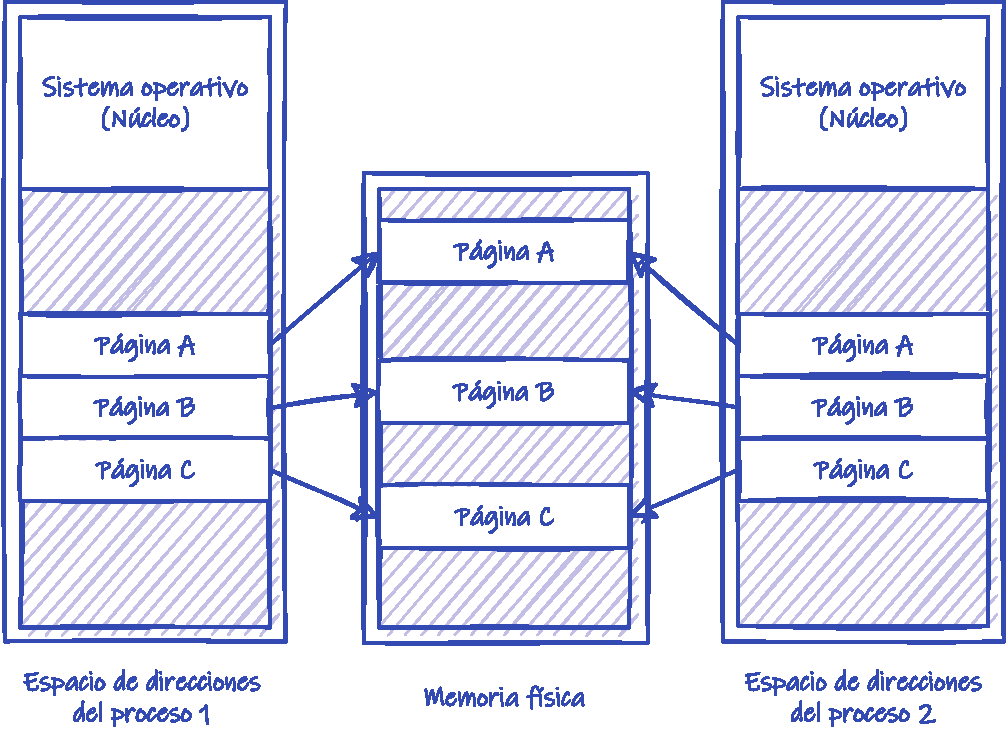
\includegraphics[width=0.8\textwidth]{media/C17_memoria_virtual/copy_on_write1.pdf}
\caption{Copy-on-write antes de que el proceso 1 modifique la página
A.}\label{fig-copy-on-write-1}
\end{figure}

\begin{enumerate}
\def\labelenumi{\arabic{enumi}.}
\item
  Cuando la llamada al sistema \{linux\_fork\} crea el nuevo proceso lo
  hace de forma que este comparta todas sus páginas con las del padre
  (véase la \hyperref[fig-copy-on-write-1]{Copy-on-write antes de que el
  proceso 1 modifique la página A.}).

  Sin el \textbf{\emph{copy-on-write}} el \{linux\_fork\} tendría que
  asignar marcos de memoria física al hijo, para a continuación copiar
  las páginas del padre en ellos. Sin embargo, con el
  \textbf{\emph{copy-on-write}} padre e hijo mapean sus páginas en los
  mismos marcos, evitando tener que asignar memoria libre.
\item
  Las páginas compartidas se marcan como \textbf{\emph{copy-on-write}}.

  Para ello se pueden marcar todas las páginas como de \textbf{solo
  lectura} en la tabla de páginas de ambos procesos y utilizar una tabla
  interna alojada en el PCB para indicar cuáles son realmente de solo
  lectura y cuáles están en \textbf{\emph{copy-on-write}}. Es importante
  destacar que realmente solo las páginas que pueden ser modificadas se
  marcan como \textbf{\emph{copy-on-write}}. Las páginas que no pueden
  ser modificadas ---por ejemplo, las que contienen el código ejecutable
  del programa--- simplemente pueden ser compartidas como de solo
  lectura por los procesos, como hemos comentado anteriormente.
\item
  Si algún proceso intenta escribir en una página
  \textbf{\emph{copy-on-write}}, la MMU genera una excepción para
  notificar el suceso al sistema operativo. Siguiendo lo indicado en el
  punto anterior, la excepción se originaría porque la página está
  marcada como de solo lectura, por lo que el sistema operativo
  comprobará si se trata de un acceso a una página
  \textbf{\emph{copy-on-write}} o a un intento real de escribir en una
  página de solo lectura. Para ello, el sistema solo tiene que mirar la
  tabla interna almacenada en el PCB. Si se ha intentado escribir en una
  página de solo lectura, el proceso ha cometido un error y generalmente
  será terminado.
\end{enumerate}

\begin{figure}
\centering
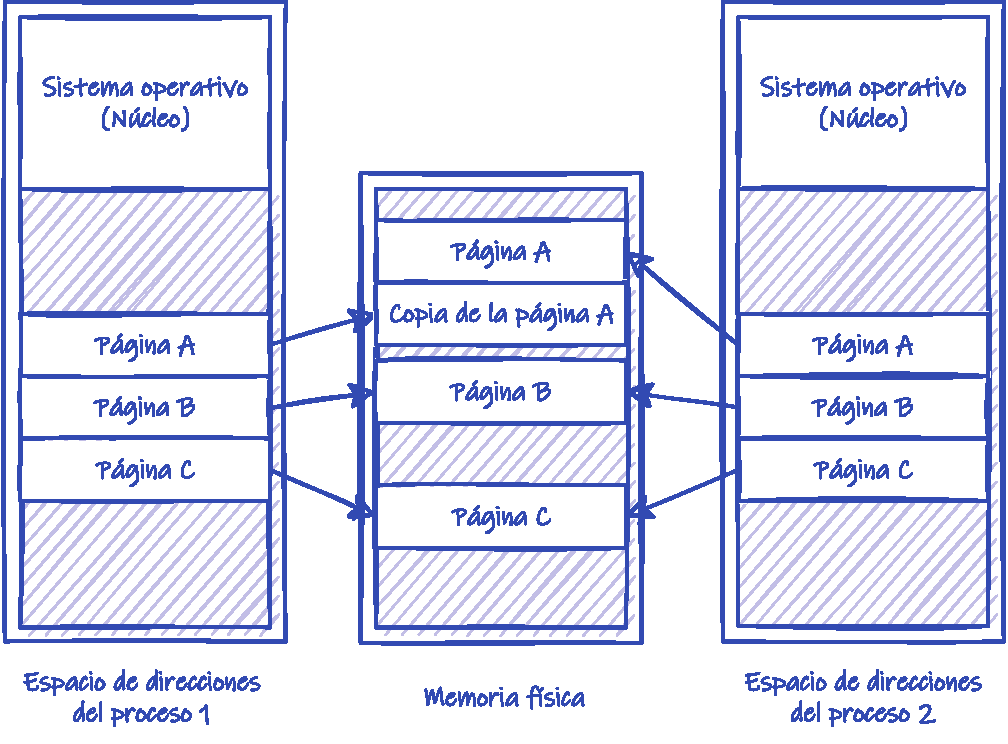
\includegraphics[width=0.8\textwidth]{media/C17_memoria_virtual/copy_on_write2.pdf}
\caption{Copy-on-write después de que el proceso 1 modifique la página
A.}\label{fig-copy-on-write-2}
\end{figure}

\begin{enumerate}
\def\labelenumi{\arabic{enumi}.}
\item
  Si el sistema detecta una escritura a una página de
  \textbf{\emph{copy-on-write}} solo tiene que copiarla en un marco
  libre y mapearlo en el espacio de direcciones del proceso (véase la
  \hyperref[fig-copy-on-write-2]{Copy-on-write después de que el proceso
  1 modifique la página A.}).

  Para esto se sustituye la página compartida por otra que contiene una
  copia, pero que ya no está compartida. Obviamente, la nueva página
  debe ser marcada como de escritura para que en el futuro pueda ser
  modificada por el proceso.
\item
  La página original marcada como \textbf{\emph{copy-on-write}} puede
  ser marcada como de escritura y no como \textbf{\emph{copy-on-write}},
  pero solo si no va a seguir siendo compartida. Esto es así porque una
  página marcada como \textbf{\emph{copy-on-write}} puede estar siendo
  compartida con otros procesos.
\item
  El sistema operativo puede reiniciar el proceso. A partir de ahora,
  este puede escribir en la página sin afectar al resto de los procesos.
  Sin embargo, puede seguir compartiendo otras páginas en
  \textbf{\emph{copy-on-write}}.
\end{enumerate}

El \textbf{\emph{copy-on-write}} permite ahorrar memoria y tiempo en la
creación de los procesos, puesto que solo se copian las páginas que son
modificadas por estos. Por eso se trata de una técnica común en
múltiples sistemas operativos, como por ejemplo los sistemas POSIX
modernos y Microsoft Windows.

El \textbf{\emph{copy-on-write}} es especialmente interesante si a
continuación se va a utilizar la llamada al sistema \{linux\_exec\}
puesto que si es así, copiar el espacio de direcciones completo es una
pérdida de tiempo.

El \textbf{\emph{copy-on-write}} también permite a los sistemas modernos
ahorrar memoria durante la reserva de grandes cantidades de memoria.
Cuando un proceso pide reservar páginas de memoria, generalmente los
sistemas deben proporcionar páginas con marcos sobreescritos con ceros,
para evitar exponer los datos del proceso que los utilizó anteriormente.
En previsión de esto, el sistema mantiene un marco completamente a 0 y
durante las reservas de memoria proporciona páginas en
\textbf{\emph{copy-on-write}} sobre dicho marco a 0. De esta forma, se
ahorra memoria física y tiempo de CPU, puesto que realmente no se asigna
un marco de memoria física y se pone a 0 su contenido hasta el momento
en el que el proceso intenta escribir en una página de memoria
previamente reservada.

\section{Archivos mapeados en
memoria}\label{_archivos_mapeados_en_memoria}

{} Los \textbf{archivos mapeados en memoria} permiten acceder a un
archivo como parte del espacio de direcciones virtuales de un proceso.
Algunas de las características de esta técnica son:

\begin{itemize}
\item
  Cuando una región del espacio de direcciones queda marcada para ser
  mapeada sobre una región de un archivo, se utiliza una estrategia
  similar a la comentada para el método básico de la paginación bajo
  demanda. La diferencia es que las páginas son cargadas desde dicho
  archivo y no desde el espacio de intercambio. Es decir, en un primer
  acceso a una página mapeada se produce un \textbf{fallo de página} que
  es resuelto por el sistema operativo leyendo una porción del archivo
  en el marco asignado a la página.
\item
  Esto significa que la lectura y escritura del archivo se realiza a
  través de lecturas y escrituras en la memoria, lo que simplifica el
  acceso y elimina el costo adicional de las llamadas al sistema:
  \{linux\_read\}, \{linux\_write\}, etc.
\item
  Las escrituras en disco se suelen realizar de forma asíncrona. Es
  decir, los datos no se escriben inmediatamente en disco cuando se
  modifica la página, sino que el sistema operativo comprueba
  periódicamente las páginas modificadas y las escribe en disco.
\item
  Los marcos utilizados en el mapeo pueden ser compartidos, lo que
  permite compartir los datos de los archivos. Además, se puede incluir
  soporte de \textbf{\emph{copy-on-write}}, lo que permite a los
  procesos compartir buena parte de un archivo en modo de solo lectura,
  pero disponiendo de sus propias copias de aquellas páginas que
  modifiquen.

  Indudablemente, para que los procesos puedan compartir datos es
  necesario que exista algún tipo de coordinación (véase el
  \hyperref[sincronizaciuxf3n]{???}).
\end{itemize}

\subsection{Ejemplo de mapeo de
archivos}\label{_ejemplo_de_mapeo_de_archivos}

Tanto en los sistemas POSIX como en Windows API el archivo a mapear hay
que abrirlo con la llamada al sistema destinada a ello. Por ejemplo, en
sistemas POSIX:

\begin{Shaded}
\begin{Highlighting}[]
\DataTypeTok{int}\NormalTok{ fd }\OperatorTok{=}\NormalTok{ open}\OperatorTok{(} \StringTok{"foo.txt"}\OperatorTok{,}\NormalTok{ O\_RDONLY }\OperatorTok{);}
\end{Highlighting}
\end{Shaded}

En la API POSIX con esto es suficiente para usar la llamada al sistema
\{linux\_mmap\} y mapear el archivo en memoria:

\begin{Shaded}
\begin{Highlighting}[]
\DataTypeTok{int}\NormalTok{ length }\OperatorTok{=}\NormalTok{ lseek}\OperatorTok{(}\NormalTok{ fd}\OperatorTok{,} \DecValTok{0}\OperatorTok{,}\NormalTok{ SEEK\_END }\OperatorTok{);}
\DataTypeTok{void}\OperatorTok{*}\NormalTok{ p }\OperatorTok{=}\NormalTok{ mmap}\OperatorTok{(}
\NormalTok{    NULL}\OperatorTok{,}
\NormalTok{    length}\OperatorTok{,}
\NormalTok{    PROT\_READ}\OperatorTok{,}
\NormalTok{    MAP\_SHARED}\OperatorTok{,}
\NormalTok{    fd}\OperatorTok{,}
    \DecValTok{0}
\OperatorTok{);}
\end{Highlighting}
\end{Shaded}

\begin{itemize}
\item
  Descriptor del archivo abierto con \{linux\_open\}.
\item
  La longitud de la región del archivo a mapear. Si queremos mapear todo
  el archivo, podemos usar \{linux\_lseek\} para conocer su longitud.
\item
  Si no se mapea todo el archivo, se puede indicar la posición del
  archivo donde comenzar el mapeo. Esta posición debe ser múltiplo del
  tamaño de página.
\item
  Permisos de la memoria mapeada. Deben coincidir con el modo con el que
  se abrió el archivo.
\end{itemize}

Una vez mapeado el archivo, si no se van a crear más mapeos, se puede
cerrar el descriptor de archivo con \{linux\_close\}. Y la región de
memoria mapeada se puede liberar, al terminar, con \{linux\_munmap\}.

En \{mapped\_files\_cpp\} se puede ver un ejemplo de un programa que
cuenta el número de líneas, palabra y caracteres de un archivo. Para
acceder al archivo, primero lo mapea en memoria, para así poder acceder
a su contenido sin tener que leerlo usando \{linux\_read\}. Una vez ha
terminado, libera la memoria mapeada.

Con Windows API el proceso requiere un paso más. Primero hay que usar el
manejador del archivo abierto para crear un \textbf{objeto de mapeo de
archivo} con \{win32\_createfilemapping\}. Después, el manejador
devuelto por \{win32\_createfilemapping\} es usado con
\{win32\_mapviewoffile\} para mapear el archivo en la memoria del
proceso.

Para liberar la memoria mapeada, se utiliza \{win32\_unmapviewoffile\}.
Mientras que para cerrar el manejador del \textbf{objeto de mapeo de
archivo} se usa \{win32\_closehandle\}, como es habitual.

\subsection{Mapeo de archivos en el
núcleo}\label{_mapeo_de_archivos_en_el_nuxfacleo}

Algunos sistemas operativos ofrecen el servicio de mapeo de archivos en
la memoria solo a través de una llamada al sistema concreta, permitiendo
utilizar las llamadas estándar ---\{linux\_read\}, \{linux\_write\},
etc.--- para hacer uso de la E/S tradicional. Sin embargo, muchos
sistemas modernos utilizan el mapeo en la memoria independientemente de
que se pidan o no.

Por ejemplo, en los sistemas POSIX, si un proceso utiliza llamada al
sistema \{linux\_mmap\} es porque explícitamente pide que el archivo sea
mapeado en memoria. Por tanto, el núcleo mapea el archivo en el espacio
de direcciones del proceso.

Pero en Linux, Microsoft Windows y otros sistemas operativos modernos,
adicionalmente, cuando un archivo es abierto con la llamada al sistema
estándar ---como \textbf{open}--- el archivo es mapeado en el espacio de
direcciones del núcleo y las llamadas \textbf{read} y \textbf{write} son
traducidas en accesos a la memoria en dicha región. No importa como sea
abierto el archivo. Estos sistemas tratan toda la E/S a archivos como
mapeada en memoria, permitiendo que el acceso a los mismos, tenga lugar
a través del eficiente componente de gestión de la memoria.

\section{Reemplazo de página}\label{_reemplazo_de_puxe1gina}

Hasta el momento hemos considerado que disponemos de memoria física
suficiente para atender cualquier fallo de página, pero ¿qué ocurre
cuando no quedan marcos libres?. En ese caso el código que da servicio a
la excepción de \textbf{fallo de página} debe escoger alguna página,
intercambiarla con el disco y utilizar el marco de la misma para cargar
la nueva página. Es decir, debemos modificar la función que ejecuta los
pasos descritos en el \hyperref[_paginaciuxf3n_bajo_demanda]{Paginación
bajo demanda} de la siguiente manera:

\begin{enumerate}
\def\labelenumi{\arabic{enumi}.}
\item
  Si la página es legal, debe ser cargada desde el disco.

  \begin{enumerate}
  \def\labelenumii{\alph{enumii}.}
  \item
    Buscar la localización de la página en disco.
  \item
    El núcleo debe buscar un marco de memoria libre que, por ejemplo, se
    puede escoger de la lista de marcos libres del sistema.

    \begin{enumerate}
    \def\labelenumiii{\roman{enumiii}.}
    \item
      Si hay uno, usarlo.
    \item
      Si no hay, usar un \textbf{algoritmo de reemplazo de página} para
      seleccionar una víctima.
    \item
      Escribir la víctima en el disco y cambiar las \textbf{tablas de
      páginas y de marcos libres} de acuerdo a la nueva situación. Para
      evitar mantener la CPU ocupada, el sistema debe solicitar la
      escritura de la página y poner al proceso en estado de
      \textbf{esperando}.
    \end{enumerate}
  \item
    Se solicita una operación de disco para leer la página deseada en el
    marco asignado. Para evitar mantener la CPU ocupada, el sistema debe
    solicitar la escritura de la página y poner al proceso en estado de
    \textbf{esperando}.
  \item
    Cuando la lectura del disco haya terminado, se debe modificar la
    tabla interna de páginas válidas, y la tabla de páginas para indicar
    que la página está en la memoria.
  \item
    Reiniciar la instrucción que fue interrumpida por la excepción.
  \end{enumerate}
\end{enumerate}

Es importante destacar que en caso de \textbf{reemplazo} se necesita
realizar dos accesos al disco. Esto se puede evitar utilizando un
\textbf{bit de modificado}{} asociado a cada entrada en la \textbf{tabla
de páginas}:

\begin{itemize}
\item
  Este bit es puesto a 1 por el hardware cuando se escribe en la página.
\item
  Se puede evitar escribir en disco aquellas páginas que tienen este bit
  a 0 cuando son seleccionadas para reemplazo, siempre que el contenido
  de la página no haya sido sobrescrito por otra en el espacio de
  intercambio.
\end{itemize}

En general, para implementar la paginación bajo demanda necesitamos:

\begin{itemize}
\item
  Un \textbf{algoritmo de asignación de marcos}, que se encarga de
  asignar los marcos a los procesos.
\item
  Un \textbf{algoritmo de reemplazo de página} para seleccionar qué
  página reemplazamos cuando no hay marcos suficientes.
\end{itemize}

Obviamente, estos algoritmos deben ser escogidos de forma que mantengan
la \textbf{tasa de fallos de página} lo más baja posible para perjudicar
en lo mínimo el rendimiento del sistema.

\subsection{Algoritmos de reemplazo de
páginas}\label{_algoritmos_de_reemplazo_de_puxe1ginas}

{} Hay muchos \textbf{algoritmos de reemplazo de página}. La cuestión es
cómo seleccionar uno en particular, sabiendo que debe tener la menor
tasa posible de \textbf{fallos de página}.

\subsubsection{Trazas de referencias}\label{_trazas_de_referencias}

{} Podemos evaluar el algoritmo utilizando una secuencia de referencias
a memoria y calculando el número de \textbf{fallos de página}. A dicha
secuencia de referencias se la denomina \textbf{trazas de referencias}.

Las trazas pueden ser obtenidas aleatoriamente u obteniéndolas a partir
de las que hace un proceso en un sistema real. Indudablemente, esta
última alternativa puede proporcionar miles de millones de referencias.
Para reducir el número de datos podemos hacer dos cosas:

\begin{itemize}
\item
  De cada referencia solo necesitamos considerar el número de página.
\item
  Si tenemos una referencia a la página \emph{p}, cualquier referencia
  inmediatamente posterior a dicha página \emph{p} nunca provocará un
  fallo de página, por lo que podemos ignorarlas. Esto no tendría por
  qué ser cierto y si consideramos que hay varios procesos en el sistema
  y unos pueden expropiar a los otros. Pero por simplicidad, ese no es
  nuestro caso.
\end{itemize}

Por ejemplo, si obtenemos la siguiente traza de un proceso particular:

\begin{verbatim}
0100, 0432, 0101, 0612, 0102, 0103, 0104, 0101, 0611, 0102, 0103, 0104, 0101, 0610, 0102, 0103, 0104, 0101, 0609, 0102, 0105
\end{verbatim}

con páginas de 100 bytes, podemos reducirla a:

\begin{verbatim}
1, 4, 1, 6, 1, 6, 1, 6, 1, 6, 1
\end{verbatim}

Indudablemente, para determinar el número de \textbf{fallos de página}
también debemos conocer el número de marcos disponibles para el proceso.

\subsubsection{Reemplazo FIFO}\label{_reemplazo_fifo}

{} {} El \textbf{algoritmo de reemplazo de páginas {}FIFO} es el más
sencillo. Funciona de la siguiente manera:

\begin{itemize}
\item
  Se asocia a cada página el instante de tiempo en que fue cargada por
  última vez.
\item
  Cuando hay que hacer reemplazo se selecciona como víctima a la página
  más antigua.
\end{itemize}

Realmente no es estrictamente necesario almacenar el instante de tiempo
en que una página fue cargada. En su lugar, las páginas en memoria
pueden ser almacenadas en una cola FIFO, puesto que así se conserva su
orden de llegada en el tiempo, que es lo que nos interesa. Esta misma
cola FIFO es utilizada en algunos algoritmos que veremos posteriormente.

Vamos a ilustrar este algoritmo con un ejemplo, donde supondremos que
tenemos 3 marcos de memoria física:

\begin{longtable}[]{@{}
  >{\raggedright\arraybackslash}p{(\linewidth - 38\tabcolsep) * \real{0.0500}}
  >{\raggedright\arraybackslash}p{(\linewidth - 38\tabcolsep) * \real{0.0500}}
  >{\raggedright\arraybackslash}p{(\linewidth - 38\tabcolsep) * \real{0.0500}}
  >{\raggedright\arraybackslash}p{(\linewidth - 38\tabcolsep) * \real{0.0500}}
  >{\raggedright\arraybackslash}p{(\linewidth - 38\tabcolsep) * \real{0.0500}}
  >{\raggedright\arraybackslash}p{(\linewidth - 38\tabcolsep) * \real{0.0500}}
  >{\raggedright\arraybackslash}p{(\linewidth - 38\tabcolsep) * \real{0.0500}}
  >{\raggedright\arraybackslash}p{(\linewidth - 38\tabcolsep) * \real{0.0500}}
  >{\raggedright\arraybackslash}p{(\linewidth - 38\tabcolsep) * \real{0.0500}}
  >{\raggedright\arraybackslash}p{(\linewidth - 38\tabcolsep) * \real{0.0500}}
  >{\raggedright\arraybackslash}p{(\linewidth - 38\tabcolsep) * \real{0.0500}}
  >{\raggedright\arraybackslash}p{(\linewidth - 38\tabcolsep) * \real{0.0500}}
  >{\raggedright\arraybackslash}p{(\linewidth - 38\tabcolsep) * \real{0.0500}}
  >{\raggedright\arraybackslash}p{(\linewidth - 38\tabcolsep) * \real{0.0500}}
  >{\raggedright\arraybackslash}p{(\linewidth - 38\tabcolsep) * \real{0.0500}}
  >{\raggedright\arraybackslash}p{(\linewidth - 38\tabcolsep) * \real{0.0500}}
  >{\raggedright\arraybackslash}p{(\linewidth - 38\tabcolsep) * \real{0.0500}}
  >{\raggedright\arraybackslash}p{(\linewidth - 38\tabcolsep) * \real{0.0500}}
  >{\raggedright\arraybackslash}p{(\linewidth - 38\tabcolsep) * \real{0.0500}}
  >{\raggedright\arraybackslash}p{(\linewidth - 38\tabcolsep) * \real{0.0500}}@{}}
\toprule\noalign{}
\begin{minipage}[b]{\linewidth}\centering
7
\end{minipage} & \begin{minipage}[b]{\linewidth}\centering
0
\end{minipage} & \begin{minipage}[b]{\linewidth}\centering
1
\end{minipage} & \begin{minipage}[b]{\linewidth}\centering
2
\end{minipage} & \begin{minipage}[b]{\linewidth}\centering
0
\end{minipage} & \begin{minipage}[b]{\linewidth}\centering
2
\end{minipage} & \begin{minipage}[b]{\linewidth}\centering
0
\end{minipage} & \begin{minipage}[b]{\linewidth}\centering
2
\end{minipage} & \begin{minipage}[b]{\linewidth}\centering
4
\end{minipage} & \begin{minipage}[b]{\linewidth}\centering
0
\end{minipage} & \begin{minipage}[b]{\linewidth}\centering
2
\end{minipage} & \begin{minipage}[b]{\linewidth}\centering
0
\end{minipage} & \begin{minipage}[b]{\linewidth}\centering
1
\end{minipage} & \begin{minipage}[b]{\linewidth}\centering
3
\end{minipage} & \begin{minipage}[b]{\linewidth}\centering
0
\end{minipage} & \begin{minipage}[b]{\linewidth}\centering
1
\end{minipage} & \begin{minipage}[b]{\linewidth}\centering
2
\end{minipage} & \begin{minipage}[b]{\linewidth}\centering
7
\end{minipage} & \begin{minipage}[b]{\linewidth}\centering
0
\end{minipage} & \begin{minipage}[b]{\linewidth}\centering
1
\end{minipage} \\
\midrule\noalign{}
\endhead
\bottomrule\noalign{}
\endlastfoot
7 & 7 & 7 & 2 & & & & & 2 & 2 & & & 1 & 1 & & & 1 & 7 & 7 & 7 \\
& 0 & 0 & 0 & & & & & 4 & 4 & & & 4 & 3 & & & 3 & 3 & 0 & 0 \\
& & 1 & 1 & & & & & 1 & 0 & & & 0 & 0 & & & 2 & 2 & 2 & 1 \\
\textbf{F} & \textbf{F} & \textbf{F} & \textbf{F} & & & & & \textbf{F} & \textbf{F} & & & \textbf{F} & \textbf{F} & & & \textbf{F} & \textbf{F} & \textbf{F} & \textbf{F} \\
\multicolumn{20}{c}{\textbf{13 fallos de página}} \\
\end{longtable}

Como se puede observar, las primeras 3 referencias generan
\textbf{fallos de página} porque se supone que los marcos no están
asignados a ninguna página. A partir de ahí se utiliza el
\textbf{algoritmo de reemplazo FIFO} para seleccionar una página cuyo
marco es utilizado para cargar la página requerida por el proceso.

El \textbf{algoritmo FIFO} no siempre tiene un buen rendimiento:

\begin{itemize}
\item
  Puesto que utiliza el orden en el tiempo, puede reemplazar tanto
  páginas que no están siendo utilizadas como páginas usadas
  frecuentemente. Sin embargo, aunque esto pase, todo seguirá
  funcionando correctamente, aunque aumentará la tasa de \textbf{fallos
  de página} enlenteciendo el sistema.
\item
  No siempre que aumenta la cantidad de memoria disponible mejora el
  rendimiento.
\end{itemize}

\begin{figure}
\centering
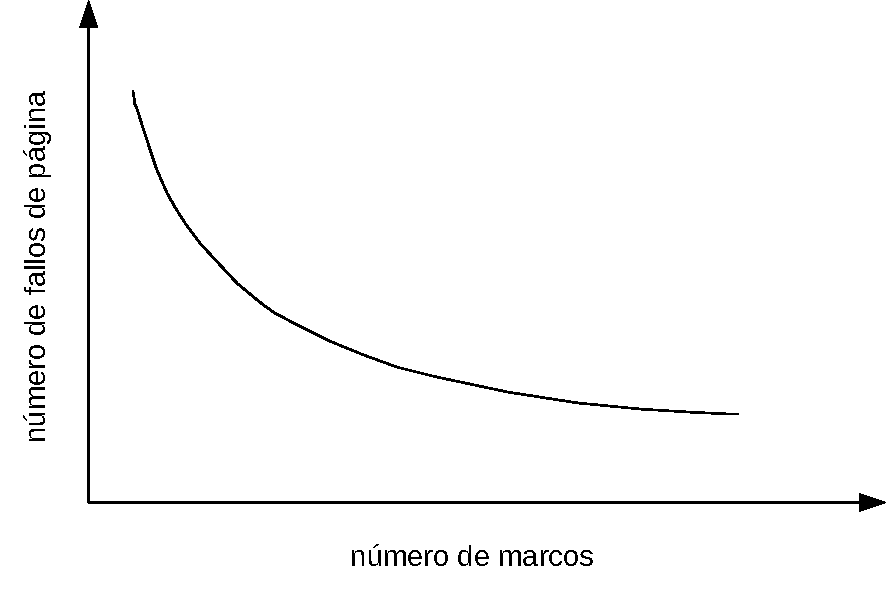
\includegraphics[width=0.8\textwidth]{media/C17_memoria_virtual/fallos_de_página_frente_a_marcos.pdf}
\caption{Fallos de página frente a número de
marcos.}\label{fig-fallos-de-puxe1gina-frente-a-marcos}
\end{figure}

Es de esperar que si el número de marcos disponibles aumenta, el número
de \textbf{fallos de página} disminuya (véase la
\hyperref[fig-fallos-de-puxe1gina-frente-a-marcos]{Fallos de página
frente a número de marcos.}). Sin embargo, con el \textbf{algoritmo
FIFO} el número de \textbf{fallos de página} puede aumentar cuando el
número de marcos disponibles se incrementa. Es lo que se conoce como la
\textbf{{}anormalidad de Belady}.

\begin{figure}
\centering
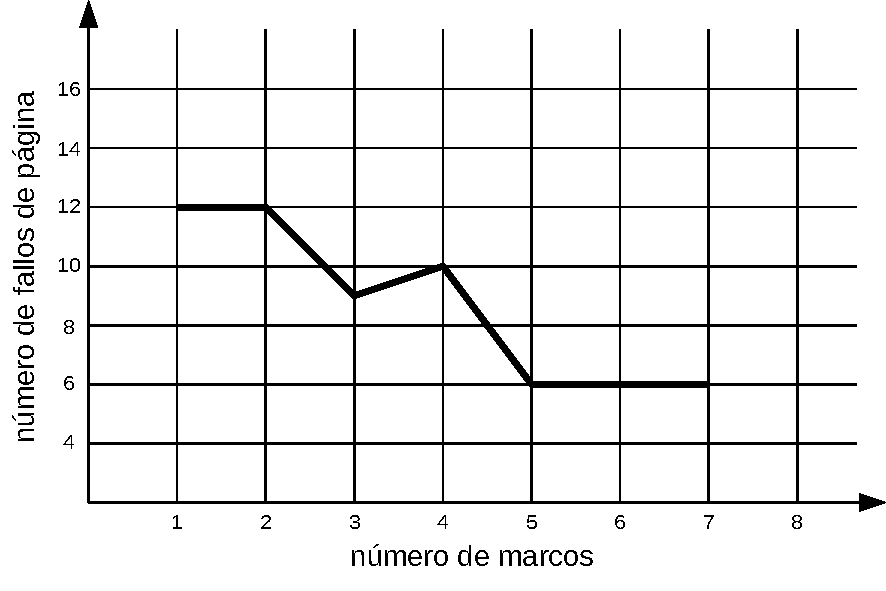
\includegraphics[width=0.8\textwidth]{media/C17_memoria_virtual/anormalidad_de_belady.pdf}
\caption{Fallos de página con el algoritmo de reemplazo
FIFO.}\label{fig-anormalidad-de-belady}
\end{figure}

Para ilustrarlo consideraremos la siguiente traza de referencias:

\begin{verbatim}
1, 2, 3, 4, 1, 2, 5, 1, 2, 3, 4, 5
\end{verbatim}

La \hyperref[fig-anormalidad-de-belady]{Fallos de página con el
algoritmo de reemplazo FIFO.} muestra la curva de \textbf{fallos de
página} frente el número de marcos. Como se puede apreciar, el número de
\textbf{fallos de página} con cuatro marcos es superior al número de
fallos con tres marcos, aunque era de esperar que el número de fallos de
páginas decrementara al aumentar el número de marcos.

\subsubsection{Reemplazo óptimo}\label{_reemplazo_uxf3ptimo}

{} {} Como resultado del descubrimiento de la \textbf{anormalidad de
Belady} se comenzó a buscar un algoritmo de reemplazo de página óptimo.
Es decir:

\begin{itemize}
\item
  Que tuviera la \textbf{tasa de fallo de página} más baja posible.
\item
  Que nunca sufra de la \textbf{anormalidad de Belady}.
\end{itemize}

Ese algoritmo existe y consiste en reemplazar la página que no va a ser
utilizada en el mayor periodo de tiempo.

\begin{longtable}[]{@{}
  >{\raggedright\arraybackslash}p{(\linewidth - 38\tabcolsep) * \real{0.0500}}
  >{\raggedright\arraybackslash}p{(\linewidth - 38\tabcolsep) * \real{0.0500}}
  >{\raggedright\arraybackslash}p{(\linewidth - 38\tabcolsep) * \real{0.0500}}
  >{\raggedright\arraybackslash}p{(\linewidth - 38\tabcolsep) * \real{0.0500}}
  >{\raggedright\arraybackslash}p{(\linewidth - 38\tabcolsep) * \real{0.0500}}
  >{\raggedright\arraybackslash}p{(\linewidth - 38\tabcolsep) * \real{0.0500}}
  >{\raggedright\arraybackslash}p{(\linewidth - 38\tabcolsep) * \real{0.0500}}
  >{\raggedright\arraybackslash}p{(\linewidth - 38\tabcolsep) * \real{0.0500}}
  >{\raggedright\arraybackslash}p{(\linewidth - 38\tabcolsep) * \real{0.0500}}
  >{\raggedright\arraybackslash}p{(\linewidth - 38\tabcolsep) * \real{0.0500}}
  >{\raggedright\arraybackslash}p{(\linewidth - 38\tabcolsep) * \real{0.0500}}
  >{\raggedright\arraybackslash}p{(\linewidth - 38\tabcolsep) * \real{0.0500}}
  >{\raggedright\arraybackslash}p{(\linewidth - 38\tabcolsep) * \real{0.0500}}
  >{\raggedright\arraybackslash}p{(\linewidth - 38\tabcolsep) * \real{0.0500}}
  >{\raggedright\arraybackslash}p{(\linewidth - 38\tabcolsep) * \real{0.0500}}
  >{\raggedright\arraybackslash}p{(\linewidth - 38\tabcolsep) * \real{0.0500}}
  >{\raggedright\arraybackslash}p{(\linewidth - 38\tabcolsep) * \real{0.0500}}
  >{\raggedright\arraybackslash}p{(\linewidth - 38\tabcolsep) * \real{0.0500}}
  >{\raggedright\arraybackslash}p{(\linewidth - 38\tabcolsep) * \real{0.0500}}
  >{\raggedright\arraybackslash}p{(\linewidth - 38\tabcolsep) * \real{0.0500}}@{}}
\toprule
\begin{minipage}[b]{\linewidth}\centering
7
\end{minipage} & \begin{minipage}[b]{\linewidth}\centering
0
\end{minipage} & \begin{minipage}[b]{\linewidth}\centering
1
\end{minipage} & \begin{minipage}[b]{\linewidth}\centering
2
\end{minipage} & \begin{minipage}[b]{\linewidth}\centering
0
\end{minipage} & \begin{minipage}[b]{\linewidth}\centering
2
\end{minipage} & \begin{minipage}[b]{\linewidth}\centering
0
\end{minipage} & \begin{minipage}[b]{\linewidth}\centering
2
\end{minipage} & \begin{minipage}[b]{\linewidth}\centering
4
\end{minipage} & \begin{minipage}[b]{\linewidth}\centering
0
\end{minipage} & \begin{minipage}[b]{\linewidth}\centering
2
\end{minipage} & \begin{minipage}[b]{\linewidth}\centering
0
\end{minipage} & \begin{minipage}[b]{\linewidth}\centering
1
\end{minipage} & \begin{minipage}[b]{\linewidth}\centering
3
\end{minipage} & \begin{minipage}[b]{\linewidth}\centering
0
\end{minipage} & \begin{minipage}[b]{\linewidth}\centering
1
\end{minipage} & \begin{minipage}[b]{\linewidth}\centering
2
\end{minipage} & \begin{minipage}[b]{\linewidth}\centering
7
\end{minipage} & \begin{minipage}[b]{\linewidth}\centering
0
\end{minipage} & \begin{minipage}[b]{\linewidth}\centering
1
\end{minipage} \\
\midrule
\endhead
\bottomrule
\endlastfoot
7 & 7 & 7 & 2 & & & & & 2 & & & & 2 & 3 & & & 2 & 2 & & \\
& 0 & 0 & 0 & & & & & 0 & & & & 0 & 0 & & & 0 & 0 & & \\
& & 1 & 1 & & & & & 4 & & & & 1 & 1 & & & 1 & 7 & & \\
\textbf{F} & \textbf{F} & \textbf{F} & \textbf{F} & & & & & \textbf{F} & & & & \textbf{F} & \textbf{F} & & & \textbf{F} & \textbf{F} & & \\
\multicolumn{20}{c}{\textbf{9 fallos de página}} \\
\end{longtable}
\par\vspace{0pt}

Desafortunadamente, el \textbf{algoritmo de reemplazo óptimo} es difícil
de implementar, puesto que necesita saber las páginas que serán
referenciadas en el futuro. Por lo que solo se usa en estudios
comparativos, con el fin de saber cuánto se aproxima al óptimo un
algoritmo de reemplazo determinado.

\subsubsection{Reemplazo LRU}\label{_reemplazo_lru}

{} {} El \textbf{algoritmo de reemplazo de página {}LRU} (\emph{Least
Recently Used}) es una aproximación del óptimo. La hipótesis es que si
una página no ha sido usada durante un gran periodo de tiempo, entonces
probablemente tampoco será utilizada en el futuro; por lo que
reemplazando la página que hace más tiempo que no se usa, nos estaríamos
aproximando al algoritmo óptimo. Vamos a ilustrarlo con un ejemplo:

\begin{longtable}[]{@{}
  >{\raggedright\arraybackslash}p{(\linewidth - 38\tabcolsep) * \real{0.0500}}
  >{\raggedright\arraybackslash}p{(\linewidth - 38\tabcolsep) * \real{0.0500}}
  >{\raggedright\arraybackslash}p{(\linewidth - 38\tabcolsep) * \real{0.0500}}
  >{\raggedright\arraybackslash}p{(\linewidth - 38\tabcolsep) * \real{0.0500}}
  >{\raggedright\arraybackslash}p{(\linewidth - 38\tabcolsep) * \real{0.0500}}
  >{\raggedright\arraybackslash}p{(\linewidth - 38\tabcolsep) * \real{0.0500}}
  >{\raggedright\arraybackslash}p{(\linewidth - 38\tabcolsep) * \real{0.0500}}
  >{\raggedright\arraybackslash}p{(\linewidth - 38\tabcolsep) * \real{0.0500}}
  >{\raggedright\arraybackslash}p{(\linewidth - 38\tabcolsep) * \real{0.0500}}
  >{\raggedright\arraybackslash}p{(\linewidth - 38\tabcolsep) * \real{0.0500}}
  >{\raggedright\arraybackslash}p{(\linewidth - 38\tabcolsep) * \real{0.0500}}
  >{\raggedright\arraybackslash}p{(\linewidth - 38\tabcolsep) * \real{0.0500}}
  >{\raggedright\arraybackslash}p{(\linewidth - 38\tabcolsep) * \real{0.0500}}
  >{\raggedright\arraybackslash}p{(\linewidth - 38\tabcolsep) * \real{0.0500}}
  >{\raggedright\arraybackslash}p{(\linewidth - 38\tabcolsep) * \real{0.0500}}
  >{\raggedright\arraybackslash}p{(\linewidth - 38\tabcolsep) * \real{0.0500}}
  >{\raggedright\arraybackslash}p{(\linewidth - 38\tabcolsep) * \real{0.0500}}
  >{\raggedright\arraybackslash}p{(\linewidth - 38\tabcolsep) * \real{0.0500}}
  >{\raggedright\arraybackslash}p{(\linewidth - 38\tabcolsep) * \real{0.0500}}
  >{\raggedright\arraybackslash}p{(\linewidth - 38\tabcolsep) * \real{0.0500}}@{}}
\toprule\noalign{}
\begin{minipage}[b]{\linewidth}\centering
7
\end{minipage} & \begin{minipage}[b]{\linewidth}\centering
0
\end{minipage} & \begin{minipage}[b]{\linewidth}\centering
1
\end{minipage} & \begin{minipage}[b]{\linewidth}\centering
2
\end{minipage} & \begin{minipage}[b]{\linewidth}\centering
0
\end{minipage} & \begin{minipage}[b]{\linewidth}\centering
2
\end{minipage} & \begin{minipage}[b]{\linewidth}\centering
0
\end{minipage} & \begin{minipage}[b]{\linewidth}\centering
2
\end{minipage} & \begin{minipage}[b]{\linewidth}\centering
4
\end{minipage} & \begin{minipage}[b]{\linewidth}\centering
0
\end{minipage} & \begin{minipage}[b]{\linewidth}\centering
2
\end{minipage} & \begin{minipage}[b]{\linewidth}\centering
0
\end{minipage} & \begin{minipage}[b]{\linewidth}\centering
1
\end{minipage} & \begin{minipage}[b]{\linewidth}\centering
3
\end{minipage} & \begin{minipage}[b]{\linewidth}\centering
0
\end{minipage} & \begin{minipage}[b]{\linewidth}\centering
1
\end{minipage} & \begin{minipage}[b]{\linewidth}\centering
2
\end{minipage} & \begin{minipage}[b]{\linewidth}\centering
7
\end{minipage} & \begin{minipage}[b]{\linewidth}\centering
0
\end{minipage} & \begin{minipage}[b]{\linewidth}\centering
1
\end{minipage} \\
\midrule\noalign{}
\endhead
\bottomrule\noalign{}
\endlastfoot
7 & 7 & 7 & 2 & & & & & 2 & & & & 2 & 3 & & & 2 & 2 & 2 & 1 \\
& 0 & 0 & 0 & & & & & 0 & & & & 0 & 0 & & & 0 & 7 & 7 & 7 \\
& & 1 & 1 & & & & & 4 & & & & 1 & 1 & & & 1 & 1 & 0 & 0 \\
\textbf{F} & \textbf{F} & \textbf{F} & \textbf{F} & & & & & \textbf{F} & & & & \textbf{F} & \textbf{F} & & & \textbf{F} & \textbf{F} & \textbf{F} & \textbf{F} \\
\multicolumn{20}{c}{\textbf{11 fallos de página}} \\
\end{longtable}

Este algoritmo se considera bastante eficiente cuando se aplica al
reemplazo de páginas, por lo que es utilizado con frecuencia.

Un detalle significativo es que necesita asociar cada página con el
momento en que fue utilizada por última vez. Aunque se pueden utilizar
interrupciones para implementarlo por software ---monitorizando cada
acceso a la memoria--- esta solución es muy ineficiente, puesto que se
necesitaría actualizar algunos datos en la memoria en cada referencia a
una página. Por ello el reemplazo LRU es inconcebible sin apoyo del
hardware.

Son posibles dos implementaciones:

\begin{itemize}
\item
  Utilizando contadores:

  \begin{enumerate}
  \def\labelenumi{\arabic{enumi}.}
  \item
    La CPU debe tener un reloj lógico o contador que se incrementa con
    cada referencia a la memoria.
  \item
    A cada página se añade un campo de \textbf{instante de uso}, que se
    almacena en la entrada de la tabla de páginas correspondiente.
  \item
    Cuando una página es referenciada, el valor del contador de la CPU
    se almacena en el campo de \textbf{instante de uso} de dicha página.
  \end{enumerate}

  Esta implementación requiere que se haga una escritura en la memoria
  con cada referencia. Además de una búsqueda por toda la tabla de
  páginas para localizar la página LRU.
\item
  Utilizando una pila:

  \begin{enumerate}
  \def\labelenumi{\arabic{enumi}.}
  \item
    Se utiliza una pila de números de página.
  \item
    Si se referencia una página, se quita el número correspondiente de
    la mitad de la pila y se inserta arriba. Debido a esto, lo mejor es
    implementarla como una lista doblemente enlazada.
  \end{enumerate}
\item
  La actualización de la pila ---que debe realizarse en cada
  referencia--- tiene mayor coste que en la implementación anterior,
  pues puede ser necesario cambiar hasta 6 punteros. Sin embargo, no es
  necesario realizar ninguna búsqueda para seleccionar la víctima del
  reemplazo, puesto que esta se puede extraer directamente del final de
  la pila.
\item
  Es una estrategia ideal para ser implementada en software o
  microcódigo.
\end{itemize}

El \textbf{algoritmo reemplazo LRU} pertenece a una clase denominada
\textbf{algoritmos de pila}, que nunca se ven afectados por la
\textbf{anormalidad de Belady}. En estos algoritmos, las páginas en
memoria en un instante dado para \emph{N} marcos son un subconjunto de
las que podría haber con \emph{N} + 1 marcos. Concretamente, en el
\textbf{algoritmo LRU} las páginas en los marcos son las \emph{N}
páginas más referenciadas recientemente. Si el número de marcos
aumentase, estas \emph{N} páginas seguirán estando en memoria, pues
siguen siendo las referenciadas más recientemente.

\subsubsection{Reemplazo LRU
aproximado}\label{_reemplazo_lru_aproximado}

Pocos sistemas tienen soporte para utilizar el \textbf{algoritmo de
reemplazo de página LRU}. Incluso en algunos casos no hay soporte de
ningún tipo, por lo que no queda más remedio que utilizar el reemplazo
FIFO.

Sin embargo, muchos proporcionan algo de ayuda en la forma de un
\textbf{bit de referencia}{}:

\begin{itemize}
\item
  Cada entrada de la tabla de páginas tiene un \textbf{bit de
  referencia}.
\item
  El hardware pone a 1 el \textbf{bit de referencia} cada vez que se
  referencia a una página.
\end{itemize}

Con el \textbf{bit de referencia} no podemos saber con exactitud el
instante, pero sí que una página ha sido referenciada recientemente.
Utilizándolo, podemos implementar diversas aproximaciones al algoritmo
LRU.

\paragraph{Reemplazo NRU}\label{_reemplazo_nru}

{} {} En el \textbf{algoritmo de reemplazo de página {}NRU} se utiliza
el \textbf{bit de referencia} de la siguiente manera:

\begin{enumerate}
\def\labelenumi{\arabic{enumi}.}
\item
  En intervalos regulares de tiempo, todos los \textbf{bits de
  referencia} son puestos a cero por el sistema operativo.
\item
  Según los procesos se van ejecutando, el \textbf{bit de referencia}
  asociado a cada página se pone a 1 por el hardware, al ser
  referenciadas.
\item
  Cuando haya que escoger una página para ser reemplazada, se intenta
  seleccionar una que no haya sido referenciada ---es decir, con el bit
  de referencia a 0---.
\item
  En caso de que haya varias alternativas entre las que elegir se puede
  utilizar el \textbf{algoritmo de reemplazo de página FIFO} o escoger
  un aleatoriamente.
\end{enumerate}

Vamos a ilustrarlo con un ejemplo:

\begin{itemize}
\item
  Utilizaremos 3 marcos de página.
\item
  Indicaremos el valor del bit de referencia con un superíndice junto al
  número de página.
\end{itemize}

No debemos olvidar que en caso de que ocurra un fallo de página, después
de la carga de la página se reinicia la instrucción que generó dicho
fallo. Por lo tanto, habrá un acceso que pondrá el \textbf{bit de
referencia a 1}.

\begin{itemize}
\item
  Marcaremos con una flecha el instante de tiempo en el que todos los
  bits de referencia se ponen a cero.
\end{itemize}

En un sistema operativo real los bits son desplazados en intervalos
fijos de tiempo. Pero esto no tiene que coincidir con una cantidad fija
de referencias en la traza, puesto que hemos eliminado las referencias
consecutivas a una misma página.

\begin{itemize}
\item
  En caso de coincidencia, utilizaremos el \textbf{reemplazo FIFO} para
  seleccionar la víctima.
\end{itemize}

\begin{longtable}[]{@{}
  >{\raggedright\arraybackslash}p{(\linewidth - 38\tabcolsep) * \real{0.0500}}
  >{\raggedright\arraybackslash}p{(\linewidth - 38\tabcolsep) * \real{0.0500}}
  >{\raggedright\arraybackslash}p{(\linewidth - 38\tabcolsep) * \real{0.0500}}
  >{\raggedright\arraybackslash}p{(\linewidth - 38\tabcolsep) * \real{0.0500}}
  >{\raggedright\arraybackslash}p{(\linewidth - 38\tabcolsep) * \real{0.0500}}
  >{\raggedright\arraybackslash}p{(\linewidth - 38\tabcolsep) * \real{0.0500}}
  >{\raggedright\arraybackslash}p{(\linewidth - 38\tabcolsep) * \real{0.0500}}
  >{\raggedright\arraybackslash}p{(\linewidth - 38\tabcolsep) * \real{0.0500}}
  >{\raggedright\arraybackslash}p{(\linewidth - 38\tabcolsep) * \real{0.0500}}
  >{\raggedright\arraybackslash}p{(\linewidth - 38\tabcolsep) * \real{0.0500}}
  >{\raggedright\arraybackslash}p{(\linewidth - 38\tabcolsep) * \real{0.0500}}
  >{\raggedright\arraybackslash}p{(\linewidth - 38\tabcolsep) * \real{0.0500}}
  >{\raggedright\arraybackslash}p{(\linewidth - 38\tabcolsep) * \real{0.0500}}
  >{\raggedright\arraybackslash}p{(\linewidth - 38\tabcolsep) * \real{0.0500}}
  >{\raggedright\arraybackslash}p{(\linewidth - 38\tabcolsep) * \real{0.0500}}
  >{\raggedright\arraybackslash}p{(\linewidth - 38\tabcolsep) * \real{0.0500}}
  >{\raggedright\arraybackslash}p{(\linewidth - 38\tabcolsep) * \real{0.0500}}
  >{\raggedright\arraybackslash}p{(\linewidth - 38\tabcolsep) * \real{0.0500}}
  >{\raggedright\arraybackslash}p{(\linewidth - 38\tabcolsep) * \real{0.0500}}
  >{\raggedright\arraybackslash}p{(\linewidth - 38\tabcolsep) * \real{0.0500}}@{}}
\toprule
\endhead
\bottomrule
\endlastfoot
& & & & \textbf{↓} & & & \textbf{↓} & & & \textbf{↓} & & & & \textbf{↓} & & & \textbf{↓} & & \\
\textbf{7} & \textbf{0} & \textbf{1} & \textbf{2} & \textbf{0} & \textbf{2} & \textbf{0} & \textbf{2} & \textbf{4} & \textbf{0} & \textbf{2} & \textbf{0} & \textbf{1} & \textbf{3} & \textbf{0} & \textbf{1} & \textbf{2} & \textbf{7} & \textbf{0} & \textbf{1} \\
7\textsuperscript{1} & 7\textsuperscript{1} & 7\textsuperscript{1} & 2\textsuperscript{1} & 2\textsuperscript{0} & 2\textsuperscript{1} & & 2\textsuperscript{1} & 2\textsuperscript{1} & 2\textsuperscript{1} & 2\textsuperscript{1} & 2\textsuperscript{1} & 2\textsuperscript{1} & 3\textsuperscript{1} & 3\textsuperscript{0} & 3\textsuperscript{0} & 2\textsuperscript{1} & 2\textsuperscript{0} & 2\textsuperscript{0} & 2\textsuperscript{0} \\
& 0\textsuperscript{1} & 0\textsuperscript{1} & 0\textsuperscript{1} & 0\textsuperscript{1} & 0\textsuperscript{1} & & 0\textsuperscript{0} & 4\textsuperscript{1} & 4\textsuperscript{1} & 4\textsuperscript{0} & 4\textsuperscript{0} & 1\textsuperscript{1} & 1\textsuperscript{1} & 1\textsuperscript{0} & 1\textsuperscript{1} & 1\textsuperscript{1} & 7\textsuperscript{1} & 7\textsuperscript{1} & 7\textsuperscript{1} \\
& & 1\textsuperscript{1} & 1\textsuperscript{1} & 1\textsuperscript{0} & 1\textsuperscript{0} & & 1\textsuperscript{0} & 1\textsuperscript{0} & 0\textsuperscript{1} & 0\textsuperscript{0} & 0\textsuperscript{1} & 0\textsuperscript{1} & 0\textsuperscript{1} & 0\textsuperscript{1} & 0\textsuperscript{1} & 0\textsuperscript{1} & 0\textsuperscript{0} & 0\textsuperscript{1} & 1\textsuperscript{1} \\
\textbf{F} & \textbf{F} & \textbf{F} & \textbf{F} & & & & & \textbf{F} & \textbf{F} & & & \textbf{F} & \textbf{F} & & & \textbf{F} & \textbf{F} & & \textbf{F} \\
\multicolumn{20}{c}{\textbf{11 fallos de página}} \\
\end{longtable}
\par\vspace{0pt}

Se puede mejorar el algoritmo anterior considerando tanto el \textbf{bit
de referencia} como el \textbf{bit de modificado}, para clasificar las
páginas en distintas categorías y escoger una página en la mejor
categoría. Este es el tipo más común de \textbf{algoritmo de reemplazo
de página NRU}, pero lo veremos en el
\hyperref[_algoritmo_de_la_segunda_oportunidad_mejorado]{Algoritmo de la
segunda oportunidad mejorado} bajo el nombre de \textbf{Algoritmo de la
segunda oportunidad mejorado}.

\paragraph{Con bits de referencia
adicionales}\label{_con_bits_de_referencia_adicionales}

Podemos obtener información adicional sobre el orden en que se realizan
las referencias, guardando los \textbf{bits de referencia} en intervalos
periódicos de tiempo. El \textbf{reemplazo LRU aproximado con bits de
referencia adicionales}, o de \textbf{envejecimiento}, consiste en lo
siguiente:

\begin{enumerate}
\def\labelenumi{\arabic{enumi}.}
\item
  Aparte del \textbf{bit de referencia}, cada página tiene un conjunto
  de \textbf{bits de referencia adicionales} ---por ejemplo, 8 bits---
  que se guardan en alguna tabla interna que mantiene el sistema
  operativo.
\item
  A intervalos regulares ---por ejemplo, cada 100 ms--- el sistema
  operativo desplaza los \textbf{bits de referencia adicionales} de cada
  página; insertando el \textbf{bit de referencia} de la página en el
  bit de orden más alto y descartando el bit de orden más bajo.
\item
  Cuando haya que escoger una página para ser reemplazada se escoge la
  que tenga el valor más pequeño en el conjunto de \textbf{bits de
  referencia adicionales}. Esto es así, puesto que dicho conjunto
  contiene la historia de referencias de la página. Por ejemplo, \{1 1 0
  0 0 1 0 0\} es más reciente que \{0 1 1 1 0 1 1 1\}.
\item
  Se puede utilizar el \textbf{algoritmo de reemplazo de página FIFO} o
  escoger un aleatoriamente, si dos páginas tienen el mismo valor.
\end{enumerate}

Vamos a ilustrarlo con un ejemplo:

\begin{itemize}
\item
  Utilizaremos 3 marcos de página.
\item
  Utilizaremos 2 bits adicionales.
\item
  Indicaremos el valor del \textbf{bit de referencia} y de los
  \textbf{bits adicionales} con un superíndice junto al número de
  página.
\item
  Marcaremos con una flecha el instante de tiempo en el que los bits son
  desplazados por el sistema operativo.
\item
  En caso de coincidencia, utilizaremos el \textbf{reemplazo FIFO} para
  seleccionar la víctima.
\end{itemize}

\begin{longtable}[]{@{}
  >{\raggedright\arraybackslash}p{(\linewidth - 38\tabcolsep) * \real{0.0500}}
  >{\raggedright\arraybackslash}p{(\linewidth - 38\tabcolsep) * \real{0.0500}}
  >{\raggedright\arraybackslash}p{(\linewidth - 38\tabcolsep) * \real{0.0500}}
  >{\raggedright\arraybackslash}p{(\linewidth - 38\tabcolsep) * \real{0.0500}}
  >{\raggedright\arraybackslash}p{(\linewidth - 38\tabcolsep) * \real{0.0500}}
  >{\raggedright\arraybackslash}p{(\linewidth - 38\tabcolsep) * \real{0.0500}}
  >{\raggedright\arraybackslash}p{(\linewidth - 38\tabcolsep) * \real{0.0500}}
  >{\raggedright\arraybackslash}p{(\linewidth - 38\tabcolsep) * \real{0.0500}}
  >{\raggedright\arraybackslash}p{(\linewidth - 38\tabcolsep) * \real{0.0500}}
  >{\raggedright\arraybackslash}p{(\linewidth - 38\tabcolsep) * \real{0.0500}}
  >{\raggedright\arraybackslash}p{(\linewidth - 38\tabcolsep) * \real{0.0500}}
  >{\raggedright\arraybackslash}p{(\linewidth - 38\tabcolsep) * \real{0.0500}}
  >{\raggedright\arraybackslash}p{(\linewidth - 38\tabcolsep) * \real{0.0500}}
  >{\raggedright\arraybackslash}p{(\linewidth - 38\tabcolsep) * \real{0.0500}}
  >{\raggedright\arraybackslash}p{(\linewidth - 38\tabcolsep) * \real{0.0500}}
  >{\raggedright\arraybackslash}p{(\linewidth - 38\tabcolsep) * \real{0.0500}}
  >{\raggedright\arraybackslash}p{(\linewidth - 38\tabcolsep) * \real{0.0500}}
  >{\raggedright\arraybackslash}p{(\linewidth - 38\tabcolsep) * \real{0.0500}}
  >{\raggedright\arraybackslash}p{(\linewidth - 38\tabcolsep) * \real{0.0500}}
  >{\raggedright\arraybackslash}p{(\linewidth - 38\tabcolsep) * \real{0.0500}}@{}}
\toprule
\endhead
\bottomrule
\endlastfoot
& & & & \textbf{↓} & & & \textbf{↓} & & & \textbf{↓} & & & & \textbf{↓} & & & \textbf{↓} & & \\
\textbf{7} & \textbf{0} & \textbf{1} & \textbf{2} & \textbf{0} & \textbf{2} & \textbf{0} & \textbf{2} & \textbf{4} & \textbf{0} & \textbf{2} & \textbf{0} & \textbf{1} & \textbf{3} & \textbf{0} & \textbf{1} & \textbf{2} & \textbf{7} & \textbf{0} & \textbf{1} \\
7\textsuperscript{1|00} & 7\textsuperscript{1|00} & 7\textsuperscript{1|00} & 2\textsuperscript{1|00} & 2\textsuperscript{0|10} & 2\textsuperscript{1|10} & 2\textsuperscript{1|10} & 2\textsuperscript{1|11} & 2\textsuperscript{1|11} & 2\textsuperscript{1|11} & 2\textsuperscript{1|11} & 2\textsuperscript{1|11} & 2\textsuperscript{1|11} & 2\textsuperscript{1|11} & 2\textsuperscript{0|11} & 2\textsuperscript{0|11} & 2\textsuperscript{1|11} & 2\textsuperscript{0|11} & 2\textsuperscript{0|11} & 2\textsuperscript{0|11} \\
& 0\textsuperscript{1|00} & 0\textsuperscript{1|00} & 0\textsuperscript{1|00} & 0\textsuperscript{1|10} & 0\textsuperscript{1|10} & 0\textsuperscript{1|10} & 0\textsuperscript{0|11} & 0\textsuperscript{0|11} & 0\textsuperscript{1|11} & 0\textsuperscript{0|11} & 0\textsuperscript{1|11} & 0\textsuperscript{1|11} & 0\textsuperscript{1|11} & 0\textsuperscript{1|11} & 0\textsuperscript{1|11} & 0\textsuperscript{1|11} & 0\textsuperscript{0|11} & 0\textsuperscript{1|11} & 0\textsuperscript{1|11} \\
& & 1\textsuperscript{1|00} & 1\textsuperscript{1|00} & 1\textsuperscript{0|10} & 1\textsuperscript{0|10} & 1\textsuperscript{0|10} & 1\textsuperscript{0|01} & 4\textsuperscript{1|00} & 4\textsuperscript{1|00} & 4\textsuperscript{0|10} & 4\textsuperscript{0|10} & 1\textsuperscript{1|00} & 3\textsuperscript{1|00} & 3\textsuperscript{0|10} & 1\textsuperscript{1|00} & 1\textsuperscript{1|00} & 7\textsuperscript{1|00} & 7\textsuperscript{1|00} & 1\textsuperscript{1|00} \\
\textbf{F} & \textbf{F} & \textbf{F} & \textbf{F} & & & & & \textbf{F} & & & & \textbf{F} & \textbf{F} & & \textbf{F} & & \textbf{F} & & \textbf{F} \\
\multicolumn{20}{c}{\textbf{10 fallos de página}} \\
\end{longtable}
\par\vspace{0pt}

El número de \textbf{bits adicionales} puede variar de una
implementación a otra, pero en cualquier caso debe ser seleccionado para
realizar la actualización lo más rápidamente posible, teniendo en cuenta
las características del hardware. En un caso extremo, el número de
\textbf{bits de referencia adicionales} podría ser cero, dejando solo el
\textbf{bit de referencia}. A este algoritmo se lo conoce como el
\textbf{algoritmo de la segunda oportunidad}.

\paragraph{Algoritmo de la segunda
oportunidad}\label{_algoritmo_de_la_segunda_oportunidad}

{} {} {} {} {} El \textbf{algoritmo de reemplazo de la segunda
oportunidad} o del \textbf{reloj} es un \textbf{algoritmo de reemplazo
de página FIFO}, pero donde una página es seleccionada considerando el
\textbf{bit de referencia}:

\begin{enumerate}
\def\labelenumi{\arabic{enumi}.}
\item
  Cuando es necesario seleccionar una víctima para reemplazo se extrae
  una página de la cola FIFO. Esta cola contiene todas las páginas con
  marcos asignados y en el orden en que fueron cargadas, como ocurre con
  el \textbf{algoritmo FIFO de reemplazo}.
\item
  Si el \textbf{bit de referencia} está a 0, se utiliza esta página para
  reemplazo.
\item
  Si el \textbf{bit de referencia} está a 1:

  \begin{enumerate}
  \def\labelenumii{\alph{enumii}.}
  \item
    Se pone el \textbf{bit de referencia} a 0 y se vuelve a insertar la
    página en el final de la cola.
  \item
    Se extrae la siguiente página del principio de la cola y se vuelve
    al punto 2.
  \end{enumerate}
\end{enumerate}

De este esquema podemos destacar algunos aspectos:

\begin{itemize}
\item
  Una página a la que se le da la segunda oportunidad, no será
  reemplazada hasta que no se le dé la segunda oportunidad a todas las
  demás; siempre que no sea referenciada antes y el \textbf{bit de
  referencia} se vuelva a poner a 1.
\item
  En el peor de los casos, cuando todas las páginas tienen sus bits a
  uno, degenera en un reemplazo FIFO.
\end{itemize}

Vamos a ilustrarlo con un ejemplo:

\begin{itemize}
\item
  Utilizaremos 3 marcos de página.
\item
  Indicaremos el valor del \textbf{bit de referencia} con un superíndice
  junto al número de página en el marco.
\item
  Indicaremos el principio de la cola con una flecha junto al número de
  página.
\end{itemize}

\begin{longtable}[]{@{}
  >{\raggedright\arraybackslash}p{(\linewidth - 38\tabcolsep) * \real{0.0500}}
  >{\raggedright\arraybackslash}p{(\linewidth - 38\tabcolsep) * \real{0.0500}}
  >{\raggedright\arraybackslash}p{(\linewidth - 38\tabcolsep) * \real{0.0500}}
  >{\raggedright\arraybackslash}p{(\linewidth - 38\tabcolsep) * \real{0.0500}}
  >{\raggedright\arraybackslash}p{(\linewidth - 38\tabcolsep) * \real{0.0500}}
  >{\raggedright\arraybackslash}p{(\linewidth - 38\tabcolsep) * \real{0.0500}}
  >{\raggedright\arraybackslash}p{(\linewidth - 38\tabcolsep) * \real{0.0500}}
  >{\raggedright\arraybackslash}p{(\linewidth - 38\tabcolsep) * \real{0.0500}}
  >{\raggedright\arraybackslash}p{(\linewidth - 38\tabcolsep) * \real{0.0500}}
  >{\raggedright\arraybackslash}p{(\linewidth - 38\tabcolsep) * \real{0.0500}}
  >{\raggedright\arraybackslash}p{(\linewidth - 38\tabcolsep) * \real{0.0500}}
  >{\raggedright\arraybackslash}p{(\linewidth - 38\tabcolsep) * \real{0.0500}}
  >{\raggedright\arraybackslash}p{(\linewidth - 38\tabcolsep) * \real{0.0500}}
  >{\raggedright\arraybackslash}p{(\linewidth - 38\tabcolsep) * \real{0.0500}}
  >{\raggedright\arraybackslash}p{(\linewidth - 38\tabcolsep) * \real{0.0500}}
  >{\raggedright\arraybackslash}p{(\linewidth - 38\tabcolsep) * \real{0.0500}}
  >{\raggedright\arraybackslash}p{(\linewidth - 38\tabcolsep) * \real{0.0500}}
  >{\raggedright\arraybackslash}p{(\linewidth - 38\tabcolsep) * \real{0.0500}}
  >{\raggedright\arraybackslash}p{(\linewidth - 38\tabcolsep) * \real{0.0500}}
  >{\raggedright\arraybackslash}p{(\linewidth - 38\tabcolsep) * \real{0.0500}}@{}}
\toprule
\begin{minipage}[b]{\linewidth}\centering
7
\end{minipage} & \begin{minipage}[b]{\linewidth}\centering
0
\end{minipage} & \begin{minipage}[b]{\linewidth}\centering
1
\end{minipage} & \begin{minipage}[b]{\linewidth}\centering
2
\end{minipage} & \begin{minipage}[b]{\linewidth}\centering
0
\end{minipage} & \begin{minipage}[b]{\linewidth}\centering
2
\end{minipage} & \begin{minipage}[b]{\linewidth}\centering
0
\end{minipage} & \begin{minipage}[b]{\linewidth}\centering
2
\end{minipage} & \begin{minipage}[b]{\linewidth}\centering
4
\end{minipage} & \begin{minipage}[b]{\linewidth}\centering
0
\end{minipage} & \begin{minipage}[b]{\linewidth}\centering
2
\end{minipage} & \begin{minipage}[b]{\linewidth}\centering
0
\end{minipage} & \begin{minipage}[b]{\linewidth}\centering
1
\end{minipage} & \begin{minipage}[b]{\linewidth}\centering
3
\end{minipage} & \begin{minipage}[b]{\linewidth}\centering
0
\end{minipage} & \begin{minipage}[b]{\linewidth}\centering
1
\end{minipage} & \begin{minipage}[b]{\linewidth}\centering
2
\end{minipage} & \begin{minipage}[b]{\linewidth}\centering
7
\end{minipage} & \begin{minipage}[b]{\linewidth}\centering
0
\end{minipage} & \begin{minipage}[b]{\linewidth}\centering
1
\end{minipage} \\
\midrule
\endhead
\bottomrule
\endlastfoot
7\textsuperscript{1} & 7\textsuperscript{1} & →7\textsuperscript{1} & 2\textsuperscript{1} & 2\textsuperscript{0} & 2\textsuperscript{1} & & 2\textsuperscript{1} & →2\textsuperscript{1} & →2\textsuperscript{1} & →2\textsuperscript{1} & →2\textsuperscript{1} & 1\textsuperscript{1} & 1\textsuperscript{1} & →1\textsuperscript{1} & →1\textsuperscript{1} & 2\textsuperscript{1} & 2\textsuperscript{1} & 2\textsuperscript{1} & →2\textsuperscript{0} \\
→ & 0\textsuperscript{1} & 0\textsuperscript{1} & →0\textsuperscript{0} & →0\textsuperscript{1} & →0\textsuperscript{1} & & →0\textsuperscript{1} & 0\textsuperscript{0} & 0\textsuperscript{1} & 0\textsuperscript{1} & 0\textsuperscript{1} & →0\textsuperscript{0} & 3\textsuperscript{1} & 3\textsuperscript{1} & 3\textsuperscript{1} & →3\textsuperscript{0} & 7\textsuperscript{1} & 7\textsuperscript{1} & 7\textsuperscript{0} \\
& → & 1\textsuperscript{1} & 1\textsuperscript{0} & 1\textsuperscript{0} & 1\textsuperscript{0} & & 1\textsuperscript{0} & 4\textsuperscript{1} & 4\textsuperscript{1} & 4\textsuperscript{1} & 4\textsuperscript{1} & 4\textsuperscript{0} & →4\textsuperscript{0} & 0\textsuperscript{1} & 0\textsuperscript{1} & 0\textsuperscript{1} & →0\textsuperscript{1} & →0\textsuperscript{1} & 1\textsuperscript{1} \\
\textbf{F} & \textbf{F} & \textbf{F} & \textbf{F} & & & & & \textbf{F} & \textbf{F} & & & \textbf{F} & \textbf{F} & & & \textbf{F} & \textbf{F} & & \textbf{F} \\
\multicolumn{20}{c}{\textbf{11 fallos de página}} \\
\end{longtable}
\par\vspace{0pt}

\paragraph{Algoritmo de la segunda oportunidad
mejorado}\label{_algoritmo_de_la_segunda_oportunidad_mejorado}

Se puede mejorar el \textbf{algoritmo de la segunda oportunidad}
considerando tanto el \textbf{bit de referencia} como el \textbf{bit de
modificado}. Algunos autores denominan a este algoritmo como
\textbf{algoritmo de la segunda oportunidad mejorado}, mientras otro lo
llaman \textbf{{}NRU}, ya que es una versión mejorada del algoritmo del
\hyperref[_reemplazo_nru]{Reemplazo NRU}.

Con esos dos bits, el sistema operativo clasifica las páginas en una de
las siguientes cuatro clases:

\begin{enumerate}
\def\labelenumi{\arabic{enumi}.}
\item
  (0,0) ni recientemente usado ni modificado. Las páginas de esta clase
  son las mejores para ser reemplazadas.
\item
  (0,1) no usado recientemente pero modificado. No es una buena
  elección, puesto que hay que escribir primero la página al disco antes
  del reemplazo.
\item
  (1,0) recientemente usado pero no modificado. Probablemente será usada
  de nuevo en un corto espacio de tiempo.
\item
  (1,1) usada y modificada. Será utilizada pronto y la página tendría
  que ser escrita a disco para ser reemplazada.
\end{enumerate}

Cuando el reemplazo de página es invocado:

\begin{itemize}
\item
  Se examina la clase a la que pertenece cada página y se reemplaza una
  página en la clase de menor importancia que no esté vacía.
  Indudablemente, deberemos examinar la lista varias veces antes de
  encontrar la página que debe ser reemplazada.
\item
  A intervalos regulares los \textbf{bits de referencia} de todas las
  páginas son puestos a cero por el sistema operativo.
\end{itemize}

En un sistema real, el sistema operativo escribe las páginas modificadas
en el almacenamiento secundario cuando está desocupado y luego pone el
\textbf{bit de modificado} a 0.

Vamos a ilustrarlo con un ejemplo:

\begin{itemize}
\item
  Utilizaremos 3 marcos de página.
\item
  El que la referencia a la memoria sea para lectura \textbf{R} o
  escritura \textbf{W} vendrá indicado junto al número de página en la
  traza.
\item
  Marcaremos con una flecha el instante de tiempo en el que todos los
  bits de referencia se ponen a cero.
\item
  Indicaremos el valor del \textbf{bit de referencia} y del \textbf{bit
  de modificado} con un superíndice junto al número de página en el
  marco.
\item
  Indicaremos el principio de la cola con una flecha junto al número de
  página. Sirve para mantener un orden en las páginas, de tal forma que
  si hay varios candidatos de la misma categoría, se escoja el primero
  encontrado. Si, por ejemplo, la elección en caso de varios candidatos
  es aleatoria, no hace falta ese puntero.
\end{itemize}

\begin{longtable}[]{@{}
  >{\raggedright\arraybackslash}p{(\linewidth - 38\tabcolsep) * \real{0.0500}}
  >{\raggedright\arraybackslash}p{(\linewidth - 38\tabcolsep) * \real{0.0500}}
  >{\raggedright\arraybackslash}p{(\linewidth - 38\tabcolsep) * \real{0.0500}}
  >{\raggedright\arraybackslash}p{(\linewidth - 38\tabcolsep) * \real{0.0500}}
  >{\raggedright\arraybackslash}p{(\linewidth - 38\tabcolsep) * \real{0.0500}}
  >{\raggedright\arraybackslash}p{(\linewidth - 38\tabcolsep) * \real{0.0500}}
  >{\raggedright\arraybackslash}p{(\linewidth - 38\tabcolsep) * \real{0.0500}}
  >{\raggedright\arraybackslash}p{(\linewidth - 38\tabcolsep) * \real{0.0500}}
  >{\raggedright\arraybackslash}p{(\linewidth - 38\tabcolsep) * \real{0.0500}}
  >{\raggedright\arraybackslash}p{(\linewidth - 38\tabcolsep) * \real{0.0500}}
  >{\raggedright\arraybackslash}p{(\linewidth - 38\tabcolsep) * \real{0.0500}}
  >{\raggedright\arraybackslash}p{(\linewidth - 38\tabcolsep) * \real{0.0500}}
  >{\raggedright\arraybackslash}p{(\linewidth - 38\tabcolsep) * \real{0.0500}}
  >{\raggedright\arraybackslash}p{(\linewidth - 38\tabcolsep) * \real{0.0500}}
  >{\raggedright\arraybackslash}p{(\linewidth - 38\tabcolsep) * \real{0.0500}}
  >{\raggedright\arraybackslash}p{(\linewidth - 38\tabcolsep) * \real{0.0500}}
  >{\raggedright\arraybackslash}p{(\linewidth - 38\tabcolsep) * \real{0.0500}}
  >{\raggedright\arraybackslash}p{(\linewidth - 38\tabcolsep) * \real{0.0500}}
  >{\raggedright\arraybackslash}p{(\linewidth - 38\tabcolsep) * \real{0.0500}}
  >{\raggedright\arraybackslash}p{(\linewidth - 38\tabcolsep) * \real{0.0500}}@{}}
\toprule\noalign{}
\endhead
\bottomrule\noalign{}
\endlastfoot
& & & & \textbf{↓} & & & \textbf{↓} & & & \textbf{↓} & & & & \textbf{↓} & & & \textbf{↓} & & \\
\textbf{7r} & \textbf{0r} & \textbf{1w} & \textbf{2r} & \textbf{0r} & \textbf{2r} & \textbf{0w} & \textbf{2r} & \textbf{4w} & \textbf{0w} & \textbf{2r} & \textbf{0r} & \textbf{1r} & \textbf{3w} & \textbf{0r} & \textbf{1r} & \textbf{2w} & \textbf{7w} & \textbf{0r} & \textbf{1r} \\
7\textsuperscript{10} & 7\textsuperscript{10} & →7\textsuperscript{10} & 2\textsuperscript{10} & 2\textsuperscript{00} & 2\textsuperscript{10} & 2\textsuperscript{10} & 2\textsuperscript{10} & 2\textsuperscript{10} & →2\textsuperscript{10} & →2\textsuperscript{10} & →2\textsuperscript{10} & 2\textsuperscript{10} & 3\textsuperscript{11} & 3\textsuperscript{01} & 3\textsuperscript{01} & 2\textsuperscript{11} & 2\textsuperscript{01} & 2\textsuperscript{01} & 1\textsuperscript{10} \\
→ & 0\textsuperscript{10} & 0\textsuperscript{10} & →0\textsuperscript{10} & →0\textsuperscript{10} & →0\textsuperscript{10} & →0\textsuperscript{11} & →0\textsuperscript{01} & 4\textsuperscript{11} & 4\textsuperscript{11} & 4\textsuperscript{01} & 4\textsuperscript{01} & 1\textsuperscript{10} & →1\textsuperscript{10} & →1\textsuperscript{00} & →1\textsuperscript{10} & →1\textsuperscript{10} & 7\textsuperscript{11} & 7\textsuperscript{11} & →7\textsuperscript{11} \\
& → & 1\textsuperscript{11} & 1\textsuperscript{11} & 1\textsuperscript{01} & 1\textsuperscript{01} & 1\textsuperscript{01} & 1\textsuperscript{01} & →1\textsuperscript{01} & 0\textsuperscript{11} & 0\textsuperscript{01} & 0\textsuperscript{11} & →0\textsuperscript{11} & 0\textsuperscript{11} & 0\textsuperscript{11} & 0\textsuperscript{11} & 0\textsuperscript{11} & →0\textsuperscript{01} & →0\textsuperscript{11} & 0\textsuperscript{11} \\
\textbf{F} & \textbf{F} & \textbf{F} & \textbf{F} & & & & & \textbf{F} & \textbf{F} & & & \textbf{F} & \textbf{F} & & & \textbf{F} & \textbf{F} & & \textbf{F} \\
\multicolumn{20}{c}{\textbf{11 fallos de página}} \\
\end{longtable}

\subsubsection{Reemplazo basado en
contador}\label{_reemplazo_basado_en_contador}

Otros algoritmos utilizan un contador del número de referencias que son
realizadas a cada página. En esos casos, la elección de la víctima se
puede realizar utilizando dos esquemas: la que tiene el valor mayor o el
menor. Ninguno de los dos es muy común, ya que su implementación es
costosa y no son una buena aproximación del óptimo.

Por lo general, la actualización del contador no la realiza la CPU, ya
que leer la entrada de la página, incrementar el contador y volver a
guardar la entrada, tiene un coste importante. En su lugar:

\begin{enumerate}
\def\labelenumi{\arabic{enumi}.}
\item
  El contador de cada página se guarda en una tabla interna.
\item
  Periódicamente el sistema operativo examina el \textbf{bit de
  referencia} de cada página y si está a 1, incrementa el contador de la
  página correspondiente.
\end{enumerate}

El mayor problema es que permite hacer el seguimiento de la frecuencia
con la que se usan las páginas, pero no tiene en cuenta el periodo
durante el que se usan. Por ejemplo, los procesos durante su
inicialización pueden usar intensamente ciertas páginas y después no
necesitarlas más. Debido a que esas páginas han sido utilizadas
intensamente, tiene un contador de referencias con un valor muy alto,
por lo que son mantenidas en memoria aunque no vaya a ser utilizadas.

La solución es utilizar el \textbf{algoritmo LRU aproximado con bits de
referencia adicionales} (véase
\hyperref[_con_bits_de_referencia_adicionales]{Con bits de referencia
adicionales}) porque tiene un coste muy similar a este y prioriza las
usadas más recientemente sobre las que fueron usadas con mucha
frecuencia en el pasado.

\paragraph{Reemplazo LFU}\label{_reemplazo_lfu}

{} {} {} {} En el \textbf{algoritmo de reemplazo de página {}LFU}
(\emph{Least Frequently Used}) o \textbf{{}NFU} (\emph{Not Frequently
Used}) se escoge la página con el contador más bajo. Esto es así, puesto
que suponemos que las páginas menos referenciadas son las que no se
están utilizando de forma más activa.

Vamos a ilustrarlo con un ejemplo:

\begin{itemize}
\item
  Indicaremos el valor de los contadores con un superíndice junto al
  número de página.
\item
  En caso de coincidencia, utilizaremos el reemplazo \textbf{FIFO} para
  seleccionar la víctima.
\end{itemize}

\begin{longtable}[]{@{}
  >{\raggedright\arraybackslash}p{(\linewidth - 38\tabcolsep) * \real{0.0500}}
  >{\raggedright\arraybackslash}p{(\linewidth - 38\tabcolsep) * \real{0.0500}}
  >{\raggedright\arraybackslash}p{(\linewidth - 38\tabcolsep) * \real{0.0500}}
  >{\raggedright\arraybackslash}p{(\linewidth - 38\tabcolsep) * \real{0.0500}}
  >{\raggedright\arraybackslash}p{(\linewidth - 38\tabcolsep) * \real{0.0500}}
  >{\raggedright\arraybackslash}p{(\linewidth - 38\tabcolsep) * \real{0.0500}}
  >{\raggedright\arraybackslash}p{(\linewidth - 38\tabcolsep) * \real{0.0500}}
  >{\raggedright\arraybackslash}p{(\linewidth - 38\tabcolsep) * \real{0.0500}}
  >{\raggedright\arraybackslash}p{(\linewidth - 38\tabcolsep) * \real{0.0500}}
  >{\raggedright\arraybackslash}p{(\linewidth - 38\tabcolsep) * \real{0.0500}}
  >{\raggedright\arraybackslash}p{(\linewidth - 38\tabcolsep) * \real{0.0500}}
  >{\raggedright\arraybackslash}p{(\linewidth - 38\tabcolsep) * \real{0.0500}}
  >{\raggedright\arraybackslash}p{(\linewidth - 38\tabcolsep) * \real{0.0500}}
  >{\raggedright\arraybackslash}p{(\linewidth - 38\tabcolsep) * \real{0.0500}}
  >{\raggedright\arraybackslash}p{(\linewidth - 38\tabcolsep) * \real{0.0500}}
  >{\raggedright\arraybackslash}p{(\linewidth - 38\tabcolsep) * \real{0.0500}}
  >{\raggedright\arraybackslash}p{(\linewidth - 38\tabcolsep) * \real{0.0500}}
  >{\raggedright\arraybackslash}p{(\linewidth - 38\tabcolsep) * \real{0.0500}}
  >{\raggedright\arraybackslash}p{(\linewidth - 38\tabcolsep) * \real{0.0500}}
  >{\raggedright\arraybackslash}p{(\linewidth - 38\tabcolsep) * \real{0.0500}}@{}}
\toprule\noalign{}
\begin{minipage}[b]{\linewidth}\centering
7
\end{minipage} & \begin{minipage}[b]{\linewidth}\centering
0
\end{minipage} & \begin{minipage}[b]{\linewidth}\centering
1
\end{minipage} & \begin{minipage}[b]{\linewidth}\centering
2
\end{minipage} & \begin{minipage}[b]{\linewidth}\centering
0
\end{minipage} & \begin{minipage}[b]{\linewidth}\centering
2
\end{minipage} & \begin{minipage}[b]{\linewidth}\centering
0
\end{minipage} & \begin{minipage}[b]{\linewidth}\centering
2
\end{minipage} & \begin{minipage}[b]{\linewidth}\centering
4
\end{minipage} & \begin{minipage}[b]{\linewidth}\centering
0
\end{minipage} & \begin{minipage}[b]{\linewidth}\centering
2
\end{minipage} & \begin{minipage}[b]{\linewidth}\centering
0
\end{minipage} & \begin{minipage}[b]{\linewidth}\centering
1
\end{minipage} & \begin{minipage}[b]{\linewidth}\centering
3
\end{minipage} & \begin{minipage}[b]{\linewidth}\centering
0
\end{minipage} & \begin{minipage}[b]{\linewidth}\centering
1
\end{minipage} & \begin{minipage}[b]{\linewidth}\centering
2
\end{minipage} & \begin{minipage}[b]{\linewidth}\centering
7
\end{minipage} & \begin{minipage}[b]{\linewidth}\centering
0
\end{minipage} & \begin{minipage}[b]{\linewidth}\centering
1
\end{minipage} \\
\midrule\noalign{}
\endhead
\bottomrule\noalign{}
\endlastfoot
7\textsuperscript{1} & 7\textsuperscript{1} & 7\textsuperscript{1} & 2\textsuperscript{1} & 2\textsuperscript{0} & 2\textsuperscript{2} & 2\textsuperscript{2} & 2\textsuperscript{3} & 2\textsuperscript{3} & 2\textsuperscript{3} & 2\textsuperscript{4} & 2\textsuperscript{4} & 2\textsuperscript{4} & 2\textsuperscript{4} & 2\textsuperscript{4} & 2\textsuperscript{4} & 2\textsuperscript{5} & 2\textsuperscript{5} & 2\textsuperscript{5} & 2\textsuperscript{5} \\
& 0\textsuperscript{1} & 0\textsuperscript{1} & 0\textsuperscript{1} & 0\textsuperscript{2} & 0\textsuperscript{2} & 0\textsuperscript{3} & 0\textsuperscript{3} & 0\textsuperscript{3} & 0\textsuperscript{4} & 0\textsuperscript{4} & 0\textsuperscript{5} & 0\textsuperscript{5} & 0\textsuperscript{5} & 0\textsuperscript{6} & 0\textsuperscript{6} & 0\textsuperscript{6} & 0\textsuperscript{6} & 0\textsuperscript{7} & 0\textsuperscript{7} \\
& & 1\textsuperscript{1} & 1\textsuperscript{1} & 1\textsuperscript{1} & 1\textsuperscript{1} & 1\textsuperscript{1} & 1\textsuperscript{1} & 4\textsuperscript{1} & 4\textsuperscript{1} & 4\textsuperscript{1} & 0\textsuperscript{1} & 1\textsuperscript{1} & 3\textsuperscript{1} & 3\textsuperscript{1} & 1\textsuperscript{1} & 1\textsuperscript{1} & 7\textsuperscript{1} & 7\textsuperscript{1} & 1\textsuperscript{1} \\
\textbf{F} & \textbf{F} & \textbf{F} & \textbf{F} & & & & & \textbf{F} & & & \textbf{F} & \textbf{F} & \textbf{F} & & \textbf{F} & \textbf{F} & \textbf{F} & & \textbf{F} \\
\multicolumn{20}{c}{\textbf{12 fallos de página}} \\
\end{longtable}

\paragraph{Reemplazo MFU}\label{_reemplazo_mfu}

En el \textbf{algoritmo de reemplazo de página {}MFU} (\emph{Most
Frequently Used}), se escoge la página con el contador más alto. Se basa
en el argumento de que la página con el contador más pequeño
probablemente acaba de ser traída, por lo que aún no ha sido utilizada.

Vamos a ilustrarlo con un ejemplo:

\begin{itemize}
\item
  Indicaremos el valor de los contadores con un superíndice junto al
  número de página.
\item
  En caso de coincidencia, utilizaremos el reemplazo \textbf{FIFO} para
  seleccionar la víctima.
\end{itemize}

\begin{longtable}[]{@{}
  >{\raggedright\arraybackslash}p{(\linewidth - 38\tabcolsep) * \real{0.0500}}
  >{\raggedright\arraybackslash}p{(\linewidth - 38\tabcolsep) * \real{0.0500}}
  >{\raggedright\arraybackslash}p{(\linewidth - 38\tabcolsep) * \real{0.0500}}
  >{\raggedright\arraybackslash}p{(\linewidth - 38\tabcolsep) * \real{0.0500}}
  >{\raggedright\arraybackslash}p{(\linewidth - 38\tabcolsep) * \real{0.0500}}
  >{\raggedright\arraybackslash}p{(\linewidth - 38\tabcolsep) * \real{0.0500}}
  >{\raggedright\arraybackslash}p{(\linewidth - 38\tabcolsep) * \real{0.0500}}
  >{\raggedright\arraybackslash}p{(\linewidth - 38\tabcolsep) * \real{0.0500}}
  >{\raggedright\arraybackslash}p{(\linewidth - 38\tabcolsep) * \real{0.0500}}
  >{\raggedright\arraybackslash}p{(\linewidth - 38\tabcolsep) * \real{0.0500}}
  >{\raggedright\arraybackslash}p{(\linewidth - 38\tabcolsep) * \real{0.0500}}
  >{\raggedright\arraybackslash}p{(\linewidth - 38\tabcolsep) * \real{0.0500}}
  >{\raggedright\arraybackslash}p{(\linewidth - 38\tabcolsep) * \real{0.0500}}
  >{\raggedright\arraybackslash}p{(\linewidth - 38\tabcolsep) * \real{0.0500}}
  >{\raggedright\arraybackslash}p{(\linewidth - 38\tabcolsep) * \real{0.0500}}
  >{\raggedright\arraybackslash}p{(\linewidth - 38\tabcolsep) * \real{0.0500}}
  >{\raggedright\arraybackslash}p{(\linewidth - 38\tabcolsep) * \real{0.0500}}
  >{\raggedright\arraybackslash}p{(\linewidth - 38\tabcolsep) * \real{0.0500}}
  >{\raggedright\arraybackslash}p{(\linewidth - 38\tabcolsep) * \real{0.0500}}
  >{\raggedright\arraybackslash}p{(\linewidth - 38\tabcolsep) * \real{0.0500}}@{}}
\toprule
\begin{minipage}[b]{\linewidth}\centering
7
\end{minipage} & \begin{minipage}[b]{\linewidth}\centering
0
\end{minipage} & \begin{minipage}[b]{\linewidth}\centering
1
\end{minipage} & \begin{minipage}[b]{\linewidth}\centering
2
\end{minipage} & \begin{minipage}[b]{\linewidth}\centering
0
\end{minipage} & \begin{minipage}[b]{\linewidth}\centering
2
\end{minipage} & \begin{minipage}[b]{\linewidth}\centering
0
\end{minipage} & \begin{minipage}[b]{\linewidth}\centering
2
\end{minipage} & \begin{minipage}[b]{\linewidth}\centering
4
\end{minipage} & \begin{minipage}[b]{\linewidth}\centering
0
\end{minipage} & \begin{minipage}[b]{\linewidth}\centering
2
\end{minipage} & \begin{minipage}[b]{\linewidth}\centering
0
\end{minipage} & \begin{minipage}[b]{\linewidth}\centering
1
\end{minipage} & \begin{minipage}[b]{\linewidth}\centering
3
\end{minipage} & \begin{minipage}[b]{\linewidth}\centering
0
\end{minipage} & \begin{minipage}[b]{\linewidth}\centering
1
\end{minipage} & \begin{minipage}[b]{\linewidth}\centering
2
\end{minipage} & \begin{minipage}[b]{\linewidth}\centering
7
\end{minipage} & \begin{minipage}[b]{\linewidth}\centering
0
\end{minipage} & \begin{minipage}[b]{\linewidth}\centering
1
\end{minipage} \\
\midrule
\endhead
\bottomrule
\endlastfoot
7\textsuperscript{1} & 7\textsuperscript{1} & 7\textsuperscript{1} & 2\textsuperscript{1} & 2\textsuperscript{1} & 2\textsuperscript{2} & 2\textsuperscript{2} & 2\textsuperscript{3} & 2\textsuperscript{3} & 0\textsuperscript{1} & 0\textsuperscript{1} & 0\textsuperscript{2} & 1\textsuperscript{1} & 1\textsuperscript{1} & 1\textsuperscript{1} & 1\textsuperscript{2} & 2\textsuperscript{1} & 2\textsuperscript{1} & 2\textsuperscript{1} & 2\textsuperscript{1} \\
& 0\textsuperscript{1} & 0\textsuperscript{1} & 0\textsuperscript{1} & 0\textsuperscript{2} & 0\textsuperscript{2} & 0\textsuperscript{3} & 0\textsuperscript{3} & 4\textsuperscript{1} & 4\textsuperscript{1} & 4\textsuperscript{1} & 4\textsuperscript{1} & 4\textsuperscript{1} & 3\textsuperscript{1} & 3\textsuperscript{1} & 3\textsuperscript{1} & 3\textsuperscript{1} & 7\textsuperscript{1} & 7\textsuperscript{1} & 7\textsuperscript{1} \\
& & 1\textsuperscript{1} & 1\textsuperscript{1} & 1\textsuperscript{1} & 1\textsuperscript{1} & 1\textsuperscript{1} & 1\textsuperscript{1} & 1\textsuperscript{1} & 1\textsuperscript{1} & 2\textsuperscript{1} & 2\textsuperscript{1} & 2\textsuperscript{1} & 2\textsuperscript{1} & 0\textsuperscript{1} & 0\textsuperscript{1} & 0\textsuperscript{1} & 0\textsuperscript{1} & 0\textsuperscript{2} & 1\textsuperscript{1} \\
\textbf{F} & \textbf{F} & \textbf{F} & \textbf{F} & & & & & \textbf{F} & \textbf{F} & \textbf{F} & & \textbf{F} & \textbf{F} & \textbf{F} & & \textbf{F} & \textbf{F} & & \textbf{F} \\
\multicolumn{20}{c}{\textbf{13 fallos de página}} \\
\end{longtable}
\par\vspace{0pt}

Por extraña que parezca esta política, suele ser más eficiente que el
\textbf{LRU} cuando se utiliza en las aplicaciones de almacenamiento de
datos, porque algunas las páginas se utilizan intensamente durante
breves periodos de tiempo, pero están un tiempo sin utilizarse.

\subsection{Algoritmos de buffering de
páginas}\label{_algoritmos_de_buffering_de_puxe1ginas}

{} Existen otros procedimientos que pueden ser utilizados, junto con
alguno de los \textbf{algoritmos de reemplazo} comentados, con el
objetivo de mejorar su eficiencia. Estos procedimientos se agrupan
dentro de lo que se denomina \textbf{algoritmos de \emph{buffering} de
páginas}.

\begin{itemize}
\item
  Se puede mantener una lista de marcos libres. Cuando se produce un
  \textbf{fallo de página} se escoge un marco de la lista y se carga la
  página, al tiempo que se selecciona una página como víctima y se copia
  al disco.

  Esto permite que el proceso se reinicie lo antes posible, sin esperar
  a que la página reemplazada sea escrita en el disco. Posteriormente,
  cuando la escritura finalice, el marco es incluido en la lista de
  marcos libres.
\item
  Recordar qué página estuvo en cada marco antes de que este pasara a la
  lista de marcos libres, sería una mejora de lo anterior. De esta forma
  las páginas podrían ser recuperadas directamente desde la lista, si
  fallara alguna antes de que su marco sea utilizado por otra página.

  Esto permite reducir los efectos de que el \textbf{algoritmo de
  reemplazo} escoja una víctima equivocada.
\item
  Se puede mantener una lista de páginas modificadas y escribirlas
  cuando el dispositivo del espacio de intercambio no esté ocupado.

  Este esquema aumenta la probabilidad de que una página no esté marcada
  como modificada ---con el \textbf{bit de modificado}--- cuando sea
  seleccionada por el algoritmo de reemplazo, evitando tener que hacer
  en ese momento la escritura en disco.
\end{itemize}

\subsection{Reemplazo local frente a
global}\label{_reemplazo_local_frente_a_global}

Cuando un proceso necesita un marco, el algoritmo de reemplazo puede,
tanto extraerlo de cualquier proceso, como ser obligado a considerar
solo aquellas páginas que pertenecen al proceso que generó el fallo. Eso
permite clasificar los algoritmos de reemplazo en dos categorías:

\begin{itemize}
\item
  En el \textbf{reemplazo local}{} solo se pueden escoger marcos de
  entre los asignados al proceso. Por tanto:

  \begin{itemize}
  \item
    El número de marcos asignados a un proceso no cambia porque ocurran
    \textbf{fallos de página}.
  \item
    El mayor inconveniente es que un proceso no puede hacer disponible a
    otros procesos los marcos de memoria que menos utiliza.
  \end{itemize}
\item
  En el \textbf{reemplazo global}{} se pueden escoger marcos de entre
  todos los del sistema, independientemente de que estén asignados a
  otro proceso o no. Por tanto:

  \begin{itemize}
  \item
    El número de marcos asignados a un proceso puede aumentar si durante
    los \textbf{fallos de página} se seleccionan marcos de otros
    procesos.
  \item
    El mayor inconveniente es que los procesos no pueden controlar su
    \textbf{tasa de fallos de página}, puesto que esta depende del
    comportamiento de los otros procesos, pudiendo afectar a su tiempo
    de ejecución de forma significativa.
  \end{itemize}
\end{itemize}

Generalmente, el \textbf{reemplazo global} proporciona mayor
rendimiento, por lo que es el método más utilizado.

\section{Asignación de marcos de
página}\label{_asignaciuxf3n_de_marcos_de_puxe1gina}

{} La cuestión que queda por resolver es cómo repartir los marcos de
memoria física libre entre los diferentes procesos, con el fin de cubrir
las necesidades de reemplazo de cada uno de ellos. Posibles soluciones a
esto serían: repartir la memoria por igual entre todos los procesos o
hacerlo en proporción a la cantidad de memoria virtual que utilizan.

Sin embargo, intuitivamente parece interesante intentar estimar de
alguna manera el \textbf{mínimo número de marcos} que realmente necesita
cada proceso. Así, si a cada proceso se le proporciona el número mínimo
de marcos necesario, el sistema podría disponer de memoria libre para
aumentar el número de procesos ---aumentando el uso de la CPU--- o para
dedicarla a otras funciones ---como es el caso de los búferes y las
cachés de E/S---.

El \textbf{mínimo número de marcos} viene establecido por diversos
factores:

\begin{itemize}
\item
  Cuando ocurre un fallo de página, la instrucción que la ha provocado,
  debe ser reiniciada después de cargar la página en un marco libre. Por
  lo tanto, un proceso debe disponer de suficientes marcos como para
  guardar todas las páginas a las que una única instrucción pueda
  acceder pues, de lo contrario, el proceso nunca podría ser reiniciado
  al fallar permanentemente en alguno de los accesos a memoria de la
  instrucción. Obviamente, este límite viene establecido por la
  arquitectura de la máquina.
\item
  Todo proceso tiene una cierta cantidad de páginas que en cada instante
  son utilizadas frecuentemente. Si el proceso no dispone de suficientes
  marcos como para alojar dichas páginas, generará fallos de página con
  demasiada frecuencia. Esto afecta negativamente al rendimiento del
  sistema, por lo que es conveniente que el sistema asigne al número de
  marcos necesario para que eso no ocurra.
\end{itemize}

En general, si se va reduciendo el número de marcos asignados a un
proceso, mucho antes de haber alcanzado el mínimo establecido por la
arquitectura, el proceso dejará de ser útil debido a la elevada
\textbf{tasa de fallos de página}, que será mayor cuanto menos marcos
tenga asignados. Cuando eso ocurre se dice que el proceso está
\textbf{hiperpaginando}.

\section{Hiperpaginación}\label{_hiperpaginaciuxf3n}

{} Como hemos comentado, la \textbf{hiperpaginación} se produce cuando
un proceso no dispone de suficientes marcos como para alojar todas las
páginas que necesita con frecuencia, por lo que la \textbf{tasa de
fallos de página} se vuelve muy elevada.

Se dice que un proceso sufre de \textbf{hiperpaginación} cuando gasta
más tiempo paginando que ejecutándose.

\subsection{Hiperpaginación en sistemas
multiprogramados}\label{_hiperpaginaciuxf3n_en_sistemas_multiprogramados}

En los primeros \textbf{sistemas multiprogramados} (\textbf{mainframes})
que implementaron la paginación bajo demanda, era posible que se diera
el siguiente caso:

\begin{enumerate}
\def\labelenumi{\arabic{enumi}.}
\item
  El sistema operativo monitorizaba el uso de la CPU. Si el uso de la
  misma era bajo, se cargaban nuevos procesos desde la \textbf{cola de
  entrada} para aumentar el número de procesos ejecutándose al mismo
  tiempo ---también llamado \textbf{{}grado de multiprogramación} en
  esos sistemas---.
\item
  Si un proceso necesitaba demasiada memoria, le podía quitar los marcos
  a otro, puesto que se utilizaba un \textbf{algoritmo de reemplazo
  global}. Esto podía ocasionar que aumentara la \textbf{tasa de fallos
  de página} del proceso que perdía los marcos.
\item
  Al aumentar los \textbf{fallos de página} el uso de la CPU decrecía,
  por lo que el sistema operativo cargaba más procesos para aumentar el
  \textbf{grado de multiprogramación} y con ello el uso de la CPU.
\item
  Esto reducía la cantidad de memoria disponible para cada proceso, lo
  que aumentaba la \textbf{tasa de fallos de páginas}, que nuevamente
  reducía el uso de la CPU.
\item
  Este mecanismo iteraba hasta reducir considerablemente el rendimiento
  del sistema.
\end{enumerate}

\begin{figure}
\centering
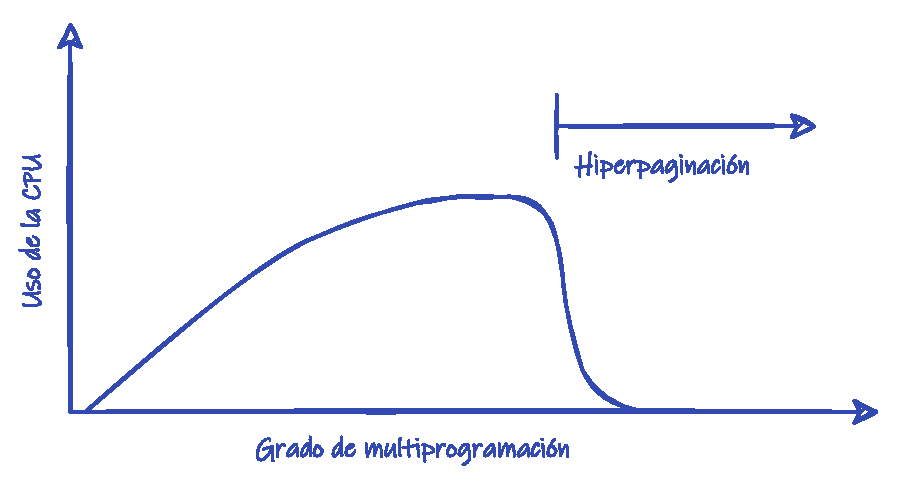
\includegraphics[width=0.8\textwidth]{media/C17_memoria_virtual/hiperpaginación.pdf}
\caption{Hiperpaginación en sistemas
multiprogramados.}\label{fig-hiperpaginaciuxf3n}
\end{figure}

El fenómeno comentado se ilustra en la
\hyperref[fig-hiperpaginaciuxf3n]{Hiperpaginación en sistemas
multiprogramados.}, donde se muestra el uso de la CPU frente al número
de procesos cargados en el sistema. Cuando esto último aumenta, el uso
de la CPU aumenta hasta alcanzar un máximo. Si el \textbf{grado de
multiprogramación} supera dicho punto, el sistema comienza a
\textbf{hiperpaginar}, por lo que el uso de la CPU disminuye
bruscamente.

Una solución es introducir un \textbf{planificador de medio plazo} que
detecte si el sistema está \textbf{hiperpaginando}, en cuyo caso
suspende y saca algunos procesos de la memoria ---reduciendo así el
\textbf{grado de multiprogramación}--- con el objeto de liberar memoria
para el resto de procesos en ejecución.

\subsection{Hiperpaginación en sistemas operativos
modernos}\label{_hiperpaginaciuxf3n_en_sistemas_operativos_modernos}

Los \textbf{sistemas de tiempo compartido} posteriores y los
\textbf{sistemas operativos modernos} no tienen ni \textbf{planificador
de largo plazo} ni \textbf{cola de entrada}, por lo que no ocurre el
efecto en cadena descrito en el caso de los sistemas multiprogramados.
Sin embargo, puede ocurrir la \textbf{hiperpaginación} si se ejecutan
demasiados procesos simultáneamente, de forma que alguno de ellos no
disponga de suficientes marcos para alojar todas las páginas que utiliza
frecuentemente (véase el
\hyperref[_modelo_del_conjunto_de_trabajo]{Modelo del conjunto de
trabajo}), aumentando así la \textbf{tasa de fallos de páginas}, hasta
el punto en que el proceso pasa más tiempo paginando que ejecutándose.

Los sistemas operativos modernos suelen carecer de \textbf{planificador
de medio plazo} por lo que, a diferencia de los \textbf{sistemas
multiprogramados}, no suspenden completamente la ejecución de algunos
procesos para reducir el consumo de memoria y evitar la
\textbf{hiperpaginación}. En su lugar, utilizan técnicas de memoria
virtual para ajustar la cantidad de marcos asignados a cada proceso,
intentando evitar la \textbf{hiperpaginación}, al tiempo que maximizan
el número de procesos que se pueden ejecutar simultaneamente.

En cualquier caso, como veremos en el
\hyperref[_modelo_del_conjunto_de_trabajo]{Modelo del conjunto de
trabajo}, habrá \textbf{hiperpaginación} si la cantidad mínima total de
marcos que necesitan todos los procesos para evitar la
\textbf{hiperpaginación} excede el número de marcos disponibles en el
sistema.

\subsection{Soluciones a la
hiperpaginación}\label{_soluciones_a_la_hiperpaginaciuxf3n}

Para el problema de la \textbf{hiperpaginación} existen diversas
soluciones:

\begin{itemize}
\item
  La principal solución es proporcionar a un proceso tantos marcos como
  le hagan falta. Como ya hemos comentado en diversas ocasiones, para
  evitar la \textbf{hiperpaginación} es necesario asignar al proceso al
  menos un número mínimo de marcos, que a priori no es conocido, ya que
  depende de cómo se comporta el proceso en su uso de la memoria. Una de
  las estrategias que pretenden estimar dicho número es el
  \textbf{modelo de conjunto de trabajo}, que veremos en la
  \hyperref[_modelo_del_conjunto_de_trabajo]{Modelo del conjunto de
  trabajo}.
\item
  Utilizar un algoritmo \textbf{de reemplazo local} puede limitiar el
  problema, pues de esta manera un proceso que \textbf{hiperpagina} no
  puede quitar marcos a otro, quizás incrementando su \textbf{tasa de
  fallos de página} y causando que también \textbf{hiperpagine}.

  Sin embargo, un algoritmo de \textbf{reemplazo local} no evita
  completamente que un proceso que \textbf{hiperpagine} afecte a otros.
  El uso intensivo del \textbf{dispositivo de intercambio}, por parte
  del proceso \textbf{hiperpagina}, puede afectar al rendimiento del
  sistema al aumentar el \textbf{tiempo de acceso efectivo} al disco.
\end{itemize}

\subsection{Modelo del conjunto de
trabajo}\label{_modelo_del_conjunto_de_trabajo}

{} Para entender el modelo de conjunto de trabajo es necesario comenzar
definiendo el \textbf{modelo de localidad}{}. El \textbf{modelo de
localidad} establece que:

\begin{itemize}
\item
  Una \textbf{{}localidad} es un conjunto de páginas que se utilizan
  juntas.
\item
  Cuando un proceso se ejecuta, se va moviendo de una \textbf{localidad}
  a otra.
\end{itemize}

Por ejemplo, cuando se invoca una función se define una nueva
\textbf{localidad}. En esta \textbf{localidad} las referencias a la
memoria se realizan: al código de la función, a las variables locales de
la misma y a algunas variables globales del programa.

Supongamos que proporcionamos a un proceso suficientes marcos como para
alojar toda su \textbf{localidad} en un momento dado. Entonces, el
proceso generará \textbf{fallos de página} hasta que todas las páginas
de su \textbf{localidad} estén cargadas. Después de eso no volverá a
fallar hasta que no cambie a una nueva \textbf{localidad}. Sin embargo,
si damos al proceso menos marcos de los que necesita su
\textbf{localidad}, este \textbf{hiperpaginará}.

El \textbf{modelo de conjunto de trabajo} es una estrategia que permite
obtener una aproximación de la \textbf{localidad} del programa y
consiste en lo siguiente:

\begin{itemize}
\item
  Definir el parámetro \emph{Δ} como el tamaño de la \textbf{ventana del
  conjunto de trabajo}.
\item
  En un instante dado, el conjunto de páginas presente en las \emph{Δ}
  últimas referencias a la memoria se consideran el \textbf{{}conjunto
  de trabajo}.
\item
  Por lo tanto, el \textbf{conjunto de trabajo} es una aproximación de
  \textbf{localidad} del programa.
\end{itemize}

Por ejemplo, dada la siguiente lista de referencias a páginas en la
memoria:

\begin{figure}
\centering
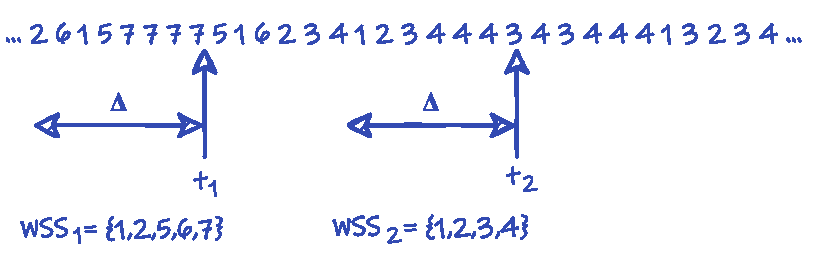
\includegraphics[width=0.8\textwidth]{media/C17_memoria_virtual/modelo_de_conjunto_de_trabajo.pdf}
\caption{}
\end{figure}

si \emph{Δ} = 10 referencias a la memoria, entonces el conjunto de
trabajo en \emph{t}\textsubscript{1} es \{1, 2, 5, 6, 7\}. Mientras que
en \emph{t}\textsubscript{2} el conjunto de trabajo es \{1, 2, 3, 4\}.

Obviamente, la precisión del \textbf{conjunto de trabajo} como
aproximación de la \textbf{localidad} del programa depende del parámetro
\emph{Δ}:

\begin{itemize}
\item
  Si \emph{Δ} es muy pequeña, el \textbf{conjunto de trabajo} no
  cubriría toda la \textbf{localidad}.
\item
  Si \emph{Δ} es muy grande, el \textbf{conjunto de trabajo} se
  superpondría a varias \textbf{localidades}.
\end{itemize}

\subsection{Uso del conjunto del trabajo para evitar la
hiperpaginación}\label{_uso_del_conjunto_del_trabajo_para_evitar_la_hiperpaginaciuxf3n}

El uso del conjunto de trabajo es bastante sencillo:

\begin{enumerate}
\def\labelenumi{\arabic{enumi}.}
\item
  Los diseñadores del sistema seleccionan \emph{Δ}.
\item
  El sistema operativo monitoriza el \textbf{conjunto de trabajo} de
  cada proceso y le asigna tantos marcos como páginas haya en el
  \textbf{conjunto de trabajo}.
\item
  Si sobran globalmente suficientes marcos:

  \begin{itemize}
  \item
    En el caso de los \textbf{sistemas multiprogramados}, otro proceso
    puede ser cargado desde la \textbf{cola de entrada} o desde el
    \textbf{dispositivo de intercambio}, si había sido suspendido
    previamente por el \textbf{planificador de medio plazo}.
  \item
    En sistemas más modernos la memoria libre puede destinarse a otros
    usos, como caché o búferes de E/S.
  \end{itemize}
\item
  Si el \textbf{tamaño del conjunto de trabajo} total \emph{WSS} crece y
  excede el número de marcos disponibles:

  \begin{itemize}
  \item
    En los \textbf{sistemas multiprogramados} con \textbf{planificador
    de medio plazo}, el sistema podría seleccionar un proceso para ser
    suspendido. Este volverá a ser cargado y reiniciado más tardel,
    cuando haya suficientes marcos libres.

    \begin{enumerate}
    \def\labelenumii{\alph{enumii}.}
    \item
      Los sistemas operativos más modernos reparten los marcos
      disponibles entre todos los procesos. Al ser la cantidad de marcos
      disponibles inferior al \emph{WSS}, es posible que algunos
      procesos \textbf{hiperpaginen}.
    \end{enumerate}
  \end{itemize}
\end{enumerate}

En la descripción anterior, el \textbf{tamaño del conjunto de trabajo}
\emph{WSS} es la suma del \textbf{tamaño de los conjuntos de trabajo}
\emph{WSS\textsubscript{i}} para cada proceso \emph{i}:

\[WSS=sum WSS_i\]

y representa la demanda total de marcos. Por eso, si \emph{WSS} es mayor
que el número de marcos disponibles, habrá \textbf{hiperpaginación}.

El sencillo algoritmo anterior permite evitar la
\textbf{hiperpaginación}. Sin embargo, el reto está en cómo mover la
\textbf{ventana del conjunto de trabajo} en cada referencia, con el fin
de volver a calcular el \textbf{conjunto de trabajo}.

Una posible aproximación es utilizar un temporizador que periódicamente
invoque a una función encargada de examinar el \textbf{bit de
referencia} de las páginas en la ventana de referencias \emph{Δ}. Es de
suponer que las páginas con el \textbf{bit de referencia} a 1 forman
parte de la \textbf{localidad} del programa y por tanto serán el
\textbf{conjunto de trabajo} a lo largo del siguiente periodo.

\section{Otras consideraciones}\label{_otras_consideraciones}

Ya hemos comentado que las principales decisiones que deben ser tomadas
en el diseño de un sistema con \textbf{paginación bajo demanda} son la
elección del \textbf{algoritmo de reemplazo} y la de la
\textbf{asignación de marcos de página}. Sin embargo, hay otras
consideraciones que deben ser tenidas en cuenta.

\subsection{Prepaginado}\label{_prepaginado}

El \textbf{{}prepaginado} es una técnica que consiste en cargar
múltiples páginas junto con la página demandada en cada \textbf{fallo de
página}.

Esas otras páginas se escogen especulativamente bajo la hipótesis de que
van a ser necesitadas por el proceso en un corto espacio de tiempo. De
manera que si la predicción es acertada, la \textbf{tasa de fallos de
página} se reduce significativamente. Esta técnica puede ser utiliza,
por ejemplo, en las siguientes situaciones:

\begin{itemize}
\item
  En la \textbf{paginación bajo demanda pura}, el sistema sabe de
  antemano que cuando se inicia un proceso siempre fallan las primeras
  páginas de código, por lo que son buenas candidatas para el
  \textbf{prepaginado}.
\item
  En el acceso secuencial a \textbf{archivos mapeados en memoria}.

  El sistema puede determinar que el acceso va a ser de tipo secuencial,
  tanto mediante el uso de técnicas heurísticas como mediante las
  opciones indicadas por el proceso en la llamada al sistema con la que
  se abrió el archivo.

  En cualquier caso, si el sistema determina que el acceso al archivo es
  secuencial, en cada \textbf{fallo de página} puede cargar tanto la
  página demanda como las siguientes, en previsión de que vayan a ser
  utilizadas por el proceso.
\end{itemize}

En general, el único inconveniente del \textbf{prepaginado} es que debe
ser ajustado para que el coste del mismo sea inferior al de servir los
\textbf{fallos de página}.

\subsection{Sobrereserva}\label{_sobrereserva}

{} {} Como las páginas de memoria de los procesos no necesitan memoria
física hasta que son referenciadas, los sistemas operativos con memoria
virtual pueden aceptar solicitudes de reserva de memoria aunque no haya
suficiente memoria física disponible. Para que el sistema operativo
pueda garantizar que siempre tiene dónde almacenar cualquier página de
cualquier proceso, debe asegurarse de que la cantidad total de memoria
reservada no exceda el espacio total disponible entre la memoria física
y el \textbf{espacio de intercambio}. Por lo general, si una petición de
reserva de memoria excede el espacio total disponible, el sistema
operativo la rechazará.

Si embargo, algunos sistemas operativos pueden aceptar solicitudes de
reserva de memoria que excedan el espacio total disponible. En estos
casos, el sistema operativo acepta la solicitud, pero no garantiza que
la memoria reservada pueda ser utilizada. Es lo que se conoce como
\textbf{sobrereserva} u \textbf{\textbf{overcommit}}.

Muchas distribuciones de Linux hacen \textbf{sobrereserva} por defecto,
aunque este comportamiento se puede desactivar. Desactivar la
\textbf{sobrereserva} es especialmente recomendable en sistemas
críticos, donde no se puede permitir que el sistema operativo termine
los procesos de forma prematura si el sistema se quedan sin espacio para
almacenar las páginas de memoria.

La \textbf{sobrereserva} es útil porque algunos programas reservan más
memoria de la que realmente necesitan, por lo que no tiene sentido que
se compruebe si hay suficiente espacio hasta que el proceso no utilice
realmente la memoria reservada. Sin embargo, tiene el riesgo de que si
se reserva más memoria de la disponible y todos los procesos intentan
utilizar buena parte de ella, el sistema se quede sin espacio para
almacenar las páginas de memoria y tenga que terminar procesos de forma
prematura para liberar espacio.

En los sistemas Linux, \textbf{{}Out Of Memory Killer} u \textbf{{}OOM
Killer} es el nombre que recibe la tarea del núcleo encargada de
terminar procesos cuando el sistema se queda sin memoria. El \textbf{OOM
Killer} selecciona los procesos a terminar en función de una serie de
criterios, como el uso de la CPU, la cantidad de memoria que consumen o
si el proceso es un servicio o un proceso de usuario.

\subsection{Aplicaciones en modo RAW}\label{_aplicaciones_en_modo_raw}

Algunas aplicaciones, cuando acceden sus datos a través de los
mecanismos de memoria virtual del sistema operativo, ofrecen peor
rendimiento del que conseguirían si este mecanismo no existiera.

El ejemplo típico, son los gestores de bases de datos, que conocen sus
necesidades de memoria y disco mejor que cualquier sistema operativo de
propósito general, por lo que salen beneficiadas si implementan sus
propios algoritmos de gestión de la memoria y de \emph{buffering} de
E/S.

Por eso muchos sistemas operativos modernos permiten que los programas
que lo soliciten puedan acceder a los discos en \textbf{modo RAW}. En el
\textbf{modo RAW} no hay sistema de archivos, ni paginación bajo
demanda, ni bloqueo de archivos, ni prepaginación, ni muchos otros
servicios del sistema operativo; por lo que dichas aplicaciones deben
implementar sus propios algoritmos de almacenamiento y gestión de la
memoria.

Sin embargo, hay que valorar muy bien las necesidades del programa antes
de optar por este modo. La mayor parte de las aplicaciones siempre
funcionan mejor utilizando los servicios convencionales ofrecidos por el
sistema operativo.

\subsection{Tamaño de las páginas}\label{_tamauxf1o_de_las_puxe1ginas}

Como ya comentamos al estudiar el método básico de paginación (véase el
\hyperref[paginaciuxf3n]{???}), una decisión de diseño importante es
escoger el tamaño adecuado para las páginas:

\begin{itemize}
\item
  \textbf{Con páginas grandes}:

  \begin{itemize}
  \item
    Se consiguen menos \textbf{fallos de páginas}. Por ejemplo, en un
    caso extremo, un proceso de 100 KiB solo podría generar un
    \textbf{fallo de página} si cada página es de 100 KiB, pero puede
    generar 102400 fallos si cada página es de 1 byte.
  \item
    Se consiguen tablas de páginas más pequeñas.
  \item
    La E/S para acceder al contenido de cada página requiere menos
    tiempo.

    En general el tiempo de transferencia es proporcional a la cantidad
    de información transferida, lo que debería beneficiar a los sistemas
    con páginas de pequeño tamaño. Sin embargo, la latencia y el tiempo
    requerido para posicionar la cabeza lectora de los discos es muy
    superior al tiempo de transferencias de datos, por lo que es más
    eficiente tener menos transferencias de mayor tamaño ---como cuando
    se usan páginas grandes--- que más transferencias de menor tamaño
    ---como cuando se usan páginas pequeñas---.
  \end{itemize}
\item
  \textbf{Con páginas pequeñas}:

  \begin{itemize}
  \item
    Se consigue tener menos \textbf{fragmentación interna} y, por tanto,
    un mejor aprovechamiento de la memoria.
  \item
    Teóricamente, se obtiene una mejor resolución para asignar y
    transferir al disco solo la memoria que realmente necesitamos. Esto
    a la larga debería redundar en menos memoria asignada y menos
    operaciones de E/S.
  \end{itemize}
\end{itemize}

En la actualidad, el tamaño de página más común es de 4 KiB en sistemas
de 32 bits y 8 KiB en los de 64 bits, ya que son adecuados para la mayor
parte de las aplicaciones. Sin embargo, muchos sistemas modernos
soportan el uso simultáneo de múltiples tamaños de página. Esto permite
que la mayor parte de las aplicaciones utilicen el tamaño estándar,
mientras las que hacen un uso intensivo de la memoria ---como es el caso
de los gestores de bases de datos--- puedan utilizar páginas de mayor
tamaño.

\subsection{Efecto de la estructura de los
programas}\label{_efecto_de_la_estructura_de_los_programas}

Los programas creados considerando la \textbf{localidad de referencia}
pueden mejorar su rendimiento en los sistemas con \textbf{paginación
bajo demanda}.

Vamos a ilustrarlo con el siguiente ejemplo de un programa que
inicializa a 0 un \emph{array} de 128 por 128 elementos.

\begin{Shaded}
\begin{Highlighting}[]
\DataTypeTok{char}\NormalTok{ data}\OperatorTok{[][]} \OperatorTok{=} \KeywordTok{new} \DataTypeTok{char}\OperatorTok{[}\DecValTok{128}\OperatorTok{][}\DecValTok{128}\OperatorTok{];}

\ControlFlowTok{for} \OperatorTok{(}\DataTypeTok{int}\NormalTok{ j }\OperatorTok{=} \DecValTok{0}\OperatorTok{;}\NormalTok{ j }\OperatorTok{\textless{}} \DecValTok{128}\OperatorTok{;} \OperatorTok{++}\NormalTok{j}\OperatorTok{)}
\OperatorTok{\{}
  \ControlFlowTok{for} \OperatorTok{(}\DataTypeTok{int}\NormalTok{ i }\OperatorTok{=} \DecValTok{0}\OperatorTok{;}\NormalTok{ i }\OperatorTok{\textless{}} \DecValTok{128}\OperatorTok{;} \OperatorTok{++}\NormalTok{i}\OperatorTok{)}
  \OperatorTok{\{}
\NormalTok{    data}\OperatorTok{[}\NormalTok{i}\OperatorTok{][}\NormalTok{j}\OperatorTok{]} \OperatorTok{=} \DecValTok{0}\OperatorTok{;}
  \OperatorTok{\}}
\OperatorTok{\}}
\end{Highlighting}
\end{Shaded}

Un \emph{array} como el indicado es almacenado en filas:

\begin{Shaded}
\begin{Highlighting}[]
\NormalTok{data}\OperatorTok{[}\DecValTok{0}\OperatorTok{][}\DecValTok{0}\OperatorTok{],}\NormalTok{ data}\OperatorTok{[}\DecValTok{0}\OperatorTok{][}\DecValTok{1}\OperatorTok{],} \OperatorTok{...,}\NormalTok{ data}\OperatorTok{[}\DecValTok{0}\OperatorTok{][}\DecValTok{127}\OperatorTok{]}
\NormalTok{data}\OperatorTok{[}\DecValTok{1}\OperatorTok{][}\DecValTok{0}\OperatorTok{],}\NormalTok{ data}\OperatorTok{[}\DecValTok{1}\OperatorTok{][}\DecValTok{1}\OperatorTok{],} \OperatorTok{...,}\NormalTok{ data}\OperatorTok{[}\DecValTok{127}\OperatorTok{][}\DecValTok{127}\OperatorTok{]}
\end{Highlighting}
\end{Shaded}

De manera que si suponemos que el tamaño de cada página es de 128 bytes,
en el mejor de los casos cada fila estará almacenada en una página. Por
lo tanto:

\begin{itemize}
\item
  Si el sistema le asigna 128 marcos o más, el proceso solo generará 128
  fallos de página.
\item
  Si el sistema operativo le asigna un solo marco, el proceso tendrá
  16 384 fallos, aproximadamente.
\end{itemize}

Sin embargo, el ejemplo sería diferente si el bucle interno del programa
recorriera las columnas del \emph{array} y no las filas:

Pues se podrían a 0 primero todos los bytes de una misma página antes de
empezar con la siguiente. Esto reduciría el número de \textbf{fallos de
página} a 128, aunque el sistema operativo solo asigne un marco al
proceso.

Por lo tanto se puede concluir que:

\begin{itemize}
\item
  La selección cuidadosa de las estructuras de datos y de programación
  pueden mejorar la \textbf{localidad}, reduciendo la \textbf{tasa de
  fallos de páginas} y el tamaño del \textbf{conjunto de trabajo}. Por
  ejemplo, las estructuras de datos tipo pila tienen buena
  \textbf{localidad}, puesto que el acceso siempre se realiza en lo alto
  de las mismas. Sin embargo, las tablas de dispersión, obviamente,
  están diseñadas para dispersar las referencias, lo que produce una
  mala \textbf{localidad}.
\item
  La elección del lenguaje de programación también puede tener efecto.
  En los lenguajes como C y C++ se utilizan punteros con frecuencia, lo
  que aleatoriza el acceso a la memoria, empeorando la \textbf{localidad
  de referencia}. Además, algunos estudios indican que los lenguajes
  orientados a objetos tienden a tener peor \textbf{localidad de
  referencia} que los que no lo son.
\item
  El compilador y el cargador también pueden tener un efecto importante:

  \begin{itemize}
  \item
    Separando el código de los datos para permitir que las páginas de
    código puedan ser de solo lectura. Esto es interesante porque las
    páginas no modificadas no tienen que ser escritas antes de ser
    reemplazadas.
  \item
    El compilador puede colocar las funciones que se llaman entre sí en
    la misma página.
  \item
    El cargador puede situar las funciones en la memoria de tal forma
    que en lo posible no crucen los bordes de las páginas.
  \end{itemize}
\end{itemize}

\subsection{Interbloqueo de E/S y bloqueo de
páginas}\label{_interbloqueo_de_es_y_bloqueo_de_puxe1ginas}

Supongamos que un proceso solicita una operación de E/S sobre el
contenido del marco de alguna de las páginas de su espacio de
direcciones y que, antes de que la operación sea realizada, la página es
reemplazada mientras el proceso está esperando. En ese caso, la
operación de E/S se podría acabar realizando sobre una página que
pertenece a un proceso diferente, ya que la operación de E/S se realiza
sobre el marco en la memoria física.

Para evitarlo existen diversas soluciones:

\begin{itemize}
\item
  Se puede utilizar la memoria del núcleo como búfer en las operaciones
  de E/S.

  En una escritura, esto obliga a la llamada al sistema a copiar los
  datos desde las páginas del proceso a la memoria del núcleo, antes de
  solicitar la operación de E/S. Mientras que en las operaciones de
  lectura sería justo al contrario.
\item
  Cada página puede tener un \textbf{bit de bloqueo} que se utiliza para
  indicar qué páginas no pueden ser seleccionadas para reemplazo.
\end{itemize}

Además los \textbf{bits de bloqueo}{} se pueden utilizar en otras muchas
situaciones:

\begin{itemize}
\item
  Bloquear las páginas del núcleo para evitar que sean reemplazadas.
\item
  Bloquear las páginas que acaban de ser cargadas.

  Esto evita que un \textbf{fallo de página} en un proceso de mayor
  prioridad pueda reclamar el marco antes de que el proceso para el que
  se cargó la página originalmente sea reiniciado, desperdiciando el
  trabajo de cargarla y provocando un nuevo \textbf{fallo de página}.

  Para implementarlo, se puede poner el \textbf{bit de bloqueo} a 1
  cuando la página se carga, volviéndolo después a poner a 0 cuando el
  proceso es planificado por primera vez, tras el \textbf{fallo de
  página} que provocó la carga de la página.
\item
  En los sistemas con \textbf{tiempo real flexible}, se suele permitir
  que las tareas de tiempo real informen de cuáles son las páginas más
  importantes, con el fin de que sean bloqueadas para evitar que puedan
  ser reemplazadas.

  Para evitar riesgos, el sistema suele considerar estas solicitudes
  como «consejos de bloqueo». De esta manera el sistema es libre de
  descartar dichos consejos si el conjunto de marcos libres llega a ser
  demasiado pequeño o si un proceso pide bloquear demasiadas páginas.
\end{itemize}

\subsection{Espacio de intercambio}\label{_espacio_de_intercambio}

La memoria virtual es una técnica que surgió para permitir ejecutar
programas que no caben en la memoria física, cuando esta era un recurso
muy limitado. Actualmente, con la cantidad de memoria física disponible
en los sistemas modernos, surge la duda de si sigue siendo necesario
disponer de espacio de intercambio.

Para responder a esa pregunta, hay que tener en cuenta que las páginas
de memoria pueden clasificarse en alguna de las siguientes categorías:

\begin{itemize}
\item
  \textbf{Páginas de código y datos del núcleo} que siempre están en
  memoria, por lo que se bloquean para evitar que sean reemplazadas.
\item
  \textbf{Páginas de para el caché de datos de E/S} con el objeto de
  acelerar futuros accesos a los mismos. Estas páginas puede ser
  reemplazadas y su contenido se puede descartar sin problemas.
\item
  \textbf{Código de programas}, que son páginas de solo lectura, por lo
  que su contenido es siempre el mismo que el del archivo del ejecutable
  que contiene al programa.
\item
  \textbf{Páginas que mapean archivos en la memoria}, cuyo contenido es
  el mismo que el de alguna región de un archivo en disco que les sirve
  de respaldo. Cuando estas páginas son de solo lectura, su contenido
  puede ser descartado sin problema. Mientras que si permiten acceso de
  escritura, las modificaciones son escritas por el sistema operativo en
  el archivo mapeado.
\item
  \textbf{Páginas anónimas}, son aquellas que no corresponden con ningún
  archivo en disco. Eso incluye la pila, el montón o la memoria
  reservada dinámicamente con \texttt{malloc()}, \texttt{new} o
  \texttt{mmap()}.

  Como el contenido de estas páginas no está respaldado en disco, si se
  reemplazan, el sistema operativo debe guardar su contenido en el
  espacio de intercambio.
\end{itemize}

Tener suficiente espacio de intercambio asegura la igualdad de trato
entre las páginas de memoria, independientemente del tipo de página que
sean. Porque si un sistema no dispone de espacio de intercambio, no
puede reemplazar \textbf{páginas anónimas}, sin importar si su contenido
es accedido con poca frecuencia, lo que puede llevar a reemplazar
páginas más importantes para el rendimiento del sistema.

Veamos las situaciones más típicas en cuanto la demanda de memoria y
como afecta al sistema tener o no espacio de intercambio:

\subsubsection{Baja demanda de memoria}\label{_baja_demanda_de_memoria}

\begin{itemize}
\item
  \textbf{Con espacio de intercambio}: El sistema puede optar
  intercambiar memoria anónima raramente utilizada, por ejemplo, para
  aumentar la cantidad de memoria caché y otras optimizaciones.
\item
  \textbf{Sin espacio de intercambio}: No se puede intercambiar la
  memoria anónima, ya que está bloqueada en la memoria. Aunque esto
  puede no presentar un problema de inmediato, en algunos casos puede
  implicar una caída en el rendimiento debido a que las páginas anónimas
  usadas con menor frecuencia no se puede utilizar para cosas más
  importantes.
\end{itemize}

\subsubsection{Demanda moderada de
memoria}\label{_demanda_moderada_de_memoria}

\begin{itemize}
\item
  \textbf{Con espacio de intercambio}: En este caso, todos los tipos de
  memoria tienen la misma posibilidad de ser reemplazadas. Esto
  significa que hay mayores posibilidades de reemplazar una página que
  no vaya a ser reclamada rápidamente de nuevo.
\item
  \textbf{Sin espacio de intercambio}: Como las páginas anónimas están
  bloqueadas en la memoria, el reemplazo tiene que ocurrir en otro tipo
  de memoria, aunque contenga peores candidatos para el reemplazo. Por
  tanto, el sistema tenderá a reducir las páginas utilizadas como caché
  de E/S, perjudicando el rendimiento del acceso al almacenamiento, y
  hay más posibilidades de reemplazar una página que se necesitará
  pronto, aumentando la probabilidad de acabar \textbf{hiperpaginando}.
\end{itemize}

\subsubsection{Alta demanda de memoria}\label{_alta_demanda_de_memoria}

\begin{itemize}
\item
  \textbf{Con espacio de intercambio}: El sistema es más resiliente a
  picos temporales de demanda de memoria, ya que tiene libertad para
  escoger las mejores páginas para intercambio. En casos de agotamiento
  severo de la memoria, tiende a prologarse el tiempo desde que comienza
  la \textbf{hiperpaginación} hasta que el sistema deja de ser usable.
\item
  \textbf{Sin espacio de intercambio}: El sistema cae en la
  \textbf{hiperpaginación} más rápidamente, ya que las páginas anónimas
  están bloqueadas en la memoria y no pueden ser reclamadas. En los
  sistemas Linux, el \textbf{OOM Killer} se activa más rápidamente para
  recuperar memoria por la vía de terminar procesos en ejecución.
\end{itemize}

\section{Interfaz de gestión de la
memoria}\label{_interfaz_de_gestiuxf3n_de_la_memoria}

Gracias a la abstracción de las técnicas de memoria virtual ---como la
paginación bajo demanda--- desde el punto de vista de los procesos, en
cualquier sistema moderno prácticamente solo hace falta una llamada al
sistema para gestionar su espacio de direcciones virtual.

En los sistemas POSIX esta llamada es \{linux\_mmap\} y en Windows API
es \{win32\_virtualalloc\}, que se usan junto a sus opuestas
\{linux\_munmap\} y \{win32\_virtualfree\}, respectivamente.

Ambas funciones permiten:

\begin{itemize}
\item
  Reservar una porción del espacio de direcciones virtual del proceso.

  La llamada solo hace la reserva de un rango de direcciones para que
  pueda ser utilizado por el proceso ---es decir, que las páginas en ese
  rango sean válidas--- siendo el componente de paginación bajo demanda,
  el responsable de asignar la memoria física que lo respalda, cuando el
  proceso acceda a esas direcciones.
\item
  Establecer permisos ---lectura, escritura y ejecución--- opciones de
  compartición entre procesos, bloqueo de páginas en la memoria física,
  páginas de gran tamaño y otras opciones, en la región de memoria
  virtual a reservar.
\end{itemize}

Además, en los sistemas POSIX, \{linux\_mmap\} se utiliza también para
mapear archivos en regiones del espacio de direcciones virtual. Mientras
que en Windows API para esa función se utilizan llamadas diferentes,
como hemos visto.

Ambas funciones ofrecen una buena cantidad de funcionalidades, pero
operan a muy bajo nivel. Por eso en ambas la página es la unidad mínima
en la gestión de la memoria. Es decir, las regiones reservadas del
espacio de direcciones virtual, siempre deben comenzar en un borde de
página y su tamaño debe ser múltiplo del tamaño de página.

El problema es cómo compatibilizar eso, con las necesidades reales de
los programas, que durante su ejecución necesitan reservar y liberar
constantemente memoria para pequeños elementos, como: \emph{arrays},
cadenas de texto, estructuras u objetos. Para esos casos, utilizar
directamente \{linux\_mmap\} o \{win32\_virtualalloc\} no es una
solución, puesto que la fragmentación interna conlleva un importante
derroche de recursos.

\subsection{Anatomía del espacio de direcciones virtual del
proceso}\label{_anatomuxeda_del_espacio_de_direcciones_virtual_del_proceso}

Los procesos pueden utilizar diversas ubicaciones dentro de su espacio
de direcciones virtual para almacenar los datos que necesitan para su
ejecución (véase la \hyperref[fig-proceso-en-memoria-completo]{Anatomía
de un proceso en memoria.}):

\begin{figure}
\centering
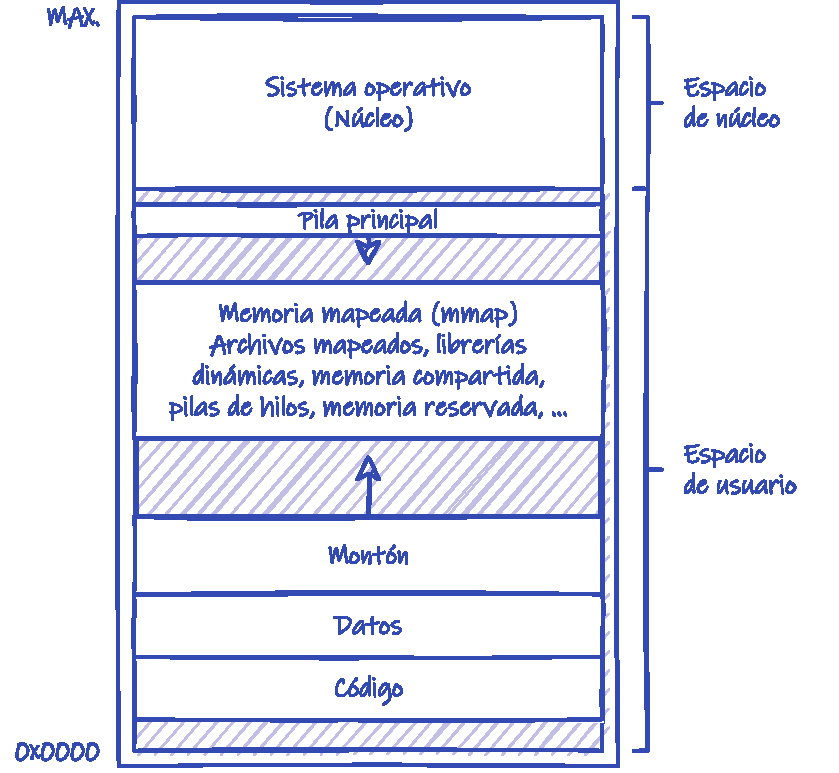
\includegraphics[width=0.8\textwidth]{media/C17_memoria_virtual/proceso_en_memoria_completo.pdf}
\caption{Anatomía de un proceso en
memoria.}\label{fig-proceso-en-memoria-completo}
\end{figure}

\begin{itemize}
\item
  Las variables y constantes globales se almacenan en el
  \textbf{segmento de datos}{}, que tiene tamaño fijo, ya que las
  dimensiones de estas variables se conocen de antemano en tiempo de
  compilación, al igual que ocurre con el código del programa.
\item
  Las variables locales y los argumentos de las funciones se almacenan
  en la \textbf{{}pila}, junto con las direcciones de retorno para
  volver de las funciones.

  Esta es la ubicación ideal para ellos, puesto que al retornar de una
  función, la pila se restablece al estado previo al que tenía cuando se
  invocó dicha función, haciendo que las variables locales y argumentos
  desaparezcan automáticamente.
\item
  Las variables reservadas dinámicamente ---por ejemplo, usando
  \{clang\_malloc\}/\{clang\_free\} en C o \{cpp\_new\}/\{cpp\_delete\}
  en C++ o Java--- se almacenan en el \textbf{{}montón}, que no es más
  una región contigua de memoria ubicada inmediatamente después del
  \textbf{segmento de datos} del proceso.
\item
  En la región entre el \textbf{montón} y la \textbf{pila} se ubican los
  \textbf{archivos mapeados en memoria}, las regiones de \textbf{memoria
  compartida}, las \textbf{librerías de enlace dinámico}, las
  \textbf{pilas} de cada hilo ---en procesos multihilo--- y, en general,
  la memoria reservada con funciones como \{linux\_mmap\} y
  \{win32\_virtualalloc\}.
\end{itemize}

Cada lenguaje de programación, debe proporcionar ---a través de su
\textbf{librería estándar}--- un mecanismo en espacio de usuario,
adecuado para la gestión en tiempo de ejecución de la memoria del
\textbf{montón} del proceso. Para eso, cada lenguaje puede utilizar su
propia implementación de dicho mecanismo o bien recurrir a la
proporcionada por la \textbf{librería del sistema}.

Por ejemplo, en los sistemas POSIX, la \textbf{librería del sistema}
proporciona su propia implementación, accesible a través de las
funciones \{clang\_malloc\} y \{clang\_free\}, que es utilizada
directamente por los programas escritos en C. Esta implementación hace
uso de \{linux\_mmap\}, pero ofrece mayor control sobre la cantidad de
memoria que podemos reservar, como veremos en el
\hyperref[_gestiuxf3n_de_la_memoria_del_montuxf3n]{Gestión de la memoria
del montón}.

Otros lenguajes de programación tienen otras interfaces para gestionar
la memoria, pero utilizan internamente las funciones \{clang\_malloc\} y
\{clang\_free\} de la \textbf{librería del sistema}. Sin embargo, este
no es el caso ni de C++ ni de Java ni de algunos otros lenguajes. En
C++, los operadores \{cpp\_new\} y \{cpp\_delete\} utilizan sus propios
algoritmos de gestión de la memoria del \textbf{montón}, más optimizados
que \{clang\_malloc\} y \{clang\_free\} para la creación y destrucción
de objetos de cualquier tamaño de manera eficiente.

En Windows API ocurre algo similar. La \textbf{librería del sistema}
proporciona su propia gestión de la memoria del \textbf{montón}, que es
accesible para cualquier programa a través de las funciones
\{win32\_heapalloc\} y \{win32\_heapfree\}, y que se implementa sobre
\{win32\_virtualalloc\}. La \textbf{librería estándar} de C utiliza, a
su vez, esas funciones para implementar \{clang\_malloc\} y
\{clang\_free\}. Lo mismo ocurre en otros lenguajes, aunque no en todos,
ya que algunos optan por implementar algoritmos más eficientes para sus
casos de uso directamente sobre \{win32\_virtualalloc\}.

\subsection{Gestión de la memoria del
montón}\label{_gestiuxf3n_de_la_memoria_del_montuxf3n}

Para ilustrar cómo se puede gestionar la memoria del \textbf{montón}
utilizaremos como ejemplo el mecanismo empleado por la \textbf{librería
del sistema} de los sistemas POSIX ---accesible a través de las
funciones \{clang\_malloc\} y \{clang\_free\}. Sin embargo, es
importante tener en cuenta que esta tarea se realiza de manera muy
similar en las implementaciones de otros sistemas operativos y lenguajes
de programación.

El funcionamiento básico de \{clang\_malloc\} sigue las siguientes
reglas:

\begin{enumerate}
\def\labelenumi{\arabic{enumi}.}
\item
  Cuando la memoria solicitada supera cierto umbral ---128 KiB en
  sistemas GNU/Linux--- es reservada directamente mediante la llamada al
  sistema \{linux\_mmap\}. Eso significa que las peticiones de gran
  tamaño realmente no consumen espacio del \textbf{montón}, si no que se
  reservan del hueco entre el \textbf{montón} y la \textbf{pila}.
\item
  Cuando un proceso hace una petición de memoria dinámica espera que el
  espacio ofrecido sea continuo en el espacio de direcciones virtual,
  por lo que la memoria del \textbf{montón} se gestiona usando un
  algoritmo de \textbf{asignación contigua de memoria} (véase
  \hyperref[_asignaciuxf3n_contigua_de_memoria]{???}) y, puesto que las
  peticiones pueden ser de tamaño variable, se utiliza con un esquema de
  \textbf{particionado dinámico}.

  Es decir, que para las peticiones que no entran en el caso anterior,
  se busca en la tabla de huecos libres y ocupados del \textbf{montón}
  uno lo suficientemente como grande para atender la petición. Se asigna
  el espacio solicitado y el resto sigue marcado como hueco libre.

  La estrategia más común de búsqueda es el \textbf{mejor ajuste},
  utilizando algún tipo de estructura de datos que mantenga los huecos
  libres ordenados por tamaño, para encontrar el de tamaño adecuado
  rápidamente.
\item
  Si no hay suficiente memoria libre contigua como para atender la
  petición, se utiliza la llamada al sistema \{linux\_mmap\}, para
  extender el tamaño del \textbf{montón} reservando una nueva región
  separada ---a veces llamada \textbf{{}arena}--- y comenzar a
  repartirla.
\end{enumerate}

En aplicaciones pequeñas, algunas implementaciones intentan ampliar
primero el espacio libre utilizando la llamada al sistema
\{linux\_brk\}, que sirve para extender el \textbf{montón} sobre la
región adyacente no asignada del espacio de direcciones virtual del
proceso. Este es el caso de la implementación estándar de
\{clang\_malloc\} en GNU/Linux.

La llamada al sistema \{linux\_brk\} ha sido eliminada del estándar
POSIX, pero algunos sistemas la mantienen por compatibilidad hacia
atrás, dado que era la forma en la que tradicionalmente se ampliaba la
memoria del \textbf{montón} en los primeros UNIX. En macOS esta llamada
se emula con una región de 4 MiB reservada con \textbf{mmap} la primera
vez que se utiliza.

La función \{clang\_calloc\} permite obtener memoria del \textbf{montón}
inicializada a 0, por lo que sigue las mismas reglas que
\{clang\_malloc\}. Cuando la petición es pequeña, obtiene la memoria del
\textbf{montón} ---extendiéndolo si fuera necesario--- para luego
ponerla manualmente a 0 antes de retornar de la función. Si la cantidad
es grande ---mayor de 128 KiB en sistemas GNU/Linux, como hemos
comentado--- obtiene la memoria llamando directamente a \{linux\_mmap\},
que ya la devuelve inicializada a 0 y que usa técnicas como el
\textbf{\emph{copy-on-write}} para ahorrar memoria física, retrasando la
asignación de marcos hasta el momento en el que el proceso comienza a
escribir realmente en la memoria reservada.

\subsection{Fragmentación}\label{_fragmentaciuxf3n}

La estrategia comentada sufre de \textbf{fragmentación interna}. En las
peticiones grandes, \{linux\_mmap\} reserva en múltiplos de tamaño de
página, por lo que siempre se puede perder cierta cantidad, aunque
pequeña en comparación al tamaño de la región reservada. En las
peticiones pequeñas, la memoria se asigna en múltiplos de una unidad
mínima ---por ejemplo, 16 o 32 bytes--- por lo que también se puede
perder cierta cantidad de memoria.

Además sufre de \textbf{fragmentación externa}, porque después de que el
proceso lleva un tiempo en ejecución, liberando y reservando memoria, el
espacio puede comenzar a quedar fraccionado en un gran número de
pequeños huecos, obligando a la librería a buscar más espacio para el
\textbf{montón}, aunque en suma haya suficiente espacio en los huecos
libres.

Esto representa un reto para los desarrolladores de aplicaciones, que
previsiblemente vayan a ejecutarse durante periodos muy largos de
tiempo. En esos casos, es común optar por librerías externas, que
implementen gestores de memoria que fragmenten menos la memoria, o
soluciones basadas en alguna forma de referencias indirectas y
recolección de basura, para ocasionalmente poder compactar la memoria
del \textbf{montón}. Esto último, es lo que hace la máquina virtual de
Java.


% ── Parte V: Gestión del almacenamiento ──────────────────
\part{Gesti\'{o}n del almacenamiento}
\input{partes/P05_preambulo}
\section{}

\textbf{Tiempo de lectura:} \{s18-reading-time\}

\section{Dispositivos de
almacenamiento}\label{_dispositivos_de_almacenamiento}

Los ordenadores pueden almacenar información en diferentes soportes de
almacenamiento ---por ejemplo, en discos magnéticos, DVD o memorias de
estado sólido---. Cada uno tiene propiedades físicas diferentes que
pasamos a comentar brevemente a continuación.

\subsection{Discos magnéticos}\label{_discos_magnuxe9ticos}

Los discos magnéticos son el tipo principal de almacenamiento
secundario, generalmente en la forma de lo que se denominan discos
duros.

\begin{figure}
\centering
\includegraphics[keepaspectratio]{media/C18_almacenamiento/disco_duro_físico.jpg}
\caption{Disco duro --- Fuente:
\href{https://commons.wikimedia.org/wiki/File:Hard_Drive_(11644168395).jpg}{Wikipedia}}\label{fig-disco-duro-fuxedsico}
\end{figure}

Tal y como se puede apreciar en la
\hyperref[fig-disco-duro-fuxedsico]{Disco duro --- Fuente: } cada unidad
está compuesta por una serie de platos de forma circular recubiertos de
material magnético. La información se almacena grabándola magnéticamente
sobre los platos, para lo cual se utilizan unas cabezas de lectura que
«flotan» tanto por encima como por debajo de cada plato.

\begin{figure}
\centering
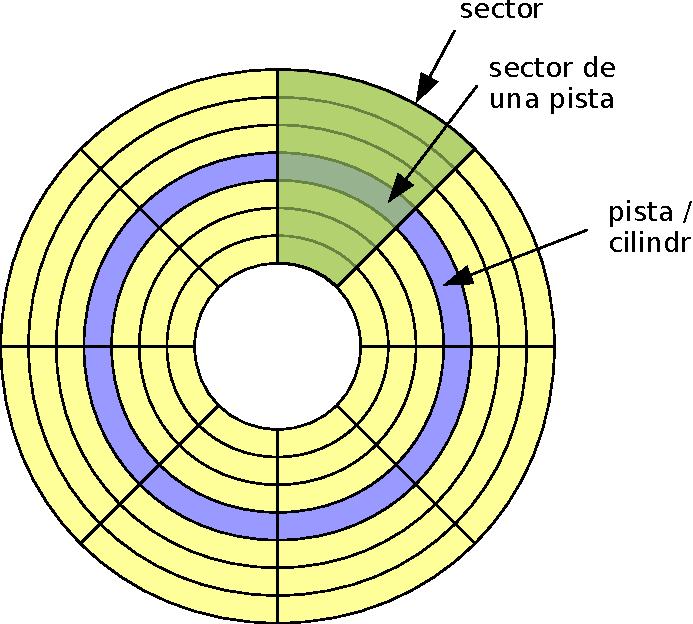
\includegraphics[width=0.8\textwidth]{media/C18_almacenamiento/disco_duro_lógico.pdf}
\caption{Estructura lógica de un disco
magnético.}\label{fig-disco-duro-luxf3gico}
\end{figure}

Desde el punto de vista lógico (véase la
\hyperref[fig-disco-duro-luxf3gico]{Estructura lógica de un disco
magnético.}) la superficie de cada plato está dividida en
\textbf{pista}{} circulares, cada una de las cuales se subdivide en
\textbf{sectores}{}. El conjunto de pistas formado por todas aquellas
que están situadas en la misma posición en los distintos platos se
denomina \textbf{{}cilindro}.

En estos dispositivos consume mucho más tiempo mover la cabeza de
lectura hasta el sector de interés, que la lectura y transferencia de
los datos almacenados a la memoria RAM. Por lo tanto, el tiempo de
acceso aleatorio al disco es mucho mayor que el de acceso secuencial.

\subsection{Discos ópticos}\label{_discos_uxf3pticos}

Los discos ópticos ---CD, DVD, BluRay, o cualquier otro medio similar---
consisten en un disco circular en el cual la información se almacena
haciendo uso de surcos microscópicos, que se leen haciendo incidir un
láser sobre una de las caras planas que lo componen.

En este tipo de discos la información se almacena siguiendo un recorrido
continuo en espiral que cubre la superficie entera del disco,
extendiéndose desde el interior hacia el exterior. Dado que el láser
siempre debe desplazarse sobre la espiral, el acceso aleatorio a los
datos es más lento que con otras tecnologías de disco.

\subsection{Memorias de estado
sólido}\label{_memorias_de_estado_suxf3lido}

Una memoria de estado sólido ---memoria USB o un SSD--- es un
dispositivo de almacenamiento que usa una memoria no volátil ---como las
\href{https://es.wikipedia.org/wiki/Memoria_flash}{memorias
\emph{flash}}--- para almacenar datos, en lugar de utilizar discos
ópticos o magnéticos.

En este tipo de memorias la información se almacena como en un vector
lineal de bytes, que se puede indexar aleatoriamente con la misma
eficiencia con la que se accede secuencialmente ---como ocurre con la
memoria RAM---. Sin embargo algunos dispositivos, de cara al resto del
sistema informático, emulan una interfaz y un modo de direccionamiento
similar al utilizado por los discos magnéticos ---es decir, usando
pistas, sectores y cilindros--- por temas de compatibilidad.

\section{Archivos y sistemas de
archivos}\label{_archivos_y_sistemas_de_archivos}

Teniendo en cuenta la gran diversidad de dispositivos de almacenamiento
que existen, para que el sistema informático sea cómodo de utilizar, el
sistema operativo proporciona una visión lógica uniforme de todos los
sistemas de almacenamiento. Es decir, abstrae las propiedades físicas de
los dispositivos de almacenamiento para definir una unidad de
almacenamiento lógico que sea útil para los usuarios. Esta unidad es el
\textbf{archivo}.

Un \textbf{{}archivo} o \textbf{{}fichero} es una colección de datos
relacionados, identificados por un nombre, que es tratada por el sistema
operativo como la unidad de información en el almacenamiento secundario.
Desde la perspectiva de los usuarios, un archivo es la unidad más
pequeña de almacenamiento. Es decir, los usuarios no pueden escribir
datos en el almacenamiento secundario a menos que estos se encuentren
dentro de un archivo.

El sistema operativo puede ofrecer esta abstracción gracias al
\textbf{sistema de archivos}{}. Este proporciona los mecanismos para el
almacenamiento de los datos y programas en archivos, tanto del propio
sistema operativo como los de todos los usuarios del sistema
informático.

Los sistemas de archivos están compuestos de dos partes claramente
diferenciadas:

\begin{itemize}
\item
  \textbf{Una colección de archivos}, cada una de las cuales almacena
  una serie de datos relacionados.
\item
  \textbf{Una colección de estructuras de metadatos}, que contienen
  información relativa a los archivos almacenados ---nombre, ubicación
  en el disco, permisos, entre otros--- y que se encarga de
  organizarlos; generalmente haciendo uso de una estructura de
  directorios.
\end{itemize}

\section{Volúmenes de datos}\label{_voluxfamenes_de_datos}

Los dispositivos de almacenamiento comentados anteriormente pueden ser
utilizados al 100\% con un único sistema de archivos. Sin embargo, en
ocasiones es interesante hacer divisiones con el objeto de disponer de
múltiples sistemas de archivos en el mismo dispositivo. Cada una de esas
divisiones es un \textbf{volumen}.

En otros casos interesa combinar divisiones o dispositivos de
almacenamiento completos para crear espacios de mayor tamaño ---también
denominados \textbf{volúmenes}--- cada una de las cuales puede albergar
un único sistema de archivos. Así que en general, utilizaremos el
término \textbf{{}volumen} para referirnos a un espacio de
almacenamiento que alberga un sistema de archivos, tanto si ese espacio
es una pequeña parte del espacio completo del dispositivo, como si se
trata de una estructura de mayor tamaño compuesta a partir de varios
dispositivos.

A continuación comentaremos brevemente las tecnologías utilizadas con
mayor frecuencia para construir estos volúmenes.

\subsection{RAID}\label{_raid}

La tecnología \textbf{{}RAID} (\emph{Redundant Array of Inexpensive
Disks}) permite combinar varios discos duros para mejorar las
prestaciones a través del paralelismo en el acceso o para mejorar la
fiabilidad a través del almacenamiento de información redundante. En
concreto se definen diversos \textbf{niveles RAID}, de entre los cuales
los más comunes son:

\begin{itemize}
\item
  En un \textbf{conjunto RAID 0} se distribuyen los datos
  equitativamente en bloques de tamaño fijo entrelazados entre dos o más
  discos, sin incluir ningún tipo de información redundante. Esto
  permite leer y escribir más datos al mismo tiempo, ya que se pueden
  enviar en paralelo peticiones a los distintos discos. Sin embargo, la
  fiabilidad es inversamente proporcional al número de discos, ya que
  para que el conjunto falle basta con que lo haga cualquiera de ellos.
\item
  En un \textbf{conjunto RAID 1} se crea una copia exacta ---en
  espejo--- de los datos en dos o más discos. El resultado es que,
  incluso con dos discos, se incrementa exponencialmente la fiabilidad
  respecto a tener uno solo, ya que para que el conjunto falle es
  necesario que lo hagan todos los discos. Adicionalmente, el
  rendimiento en las operaciones de lectura se incrementa linealmente
  con el número de copias, ya que los datos están disponibles en todos
  los discos al mismo tiempo, por lo que se pueden balancear las
  operaciones de lectura entre todos ellos.
\item
  En un \textbf{conjunto RAID 5} se distribuyen los datos
  equitativamente en bloques de tamaño fijo entrelazados entre dos o más
  discos y se utiliza uno adicional para almacenar la información de
  paridad de los bloques de una misma división. En RAID se denomina
  división o \emph{stripe} a la serie de bloques consecutivos, escogidos
  de cada uno de los discos del conjunto.

  El disco utilizado para almacenar el bloque de paridad cambia de forma
  escalonada de una división a la siguiente, de ahí que se diga que el
  bloque de paridad está distribuido. Algunos aspectos adicionales a
  tener en cuenta son que:

  \begin{itemize}
  \item
    Cada vez que se escribe un bloque de datos se debe actualizar el
    bloque de paridad. Por lo tanto las escrituras en un conjunto RAID 5
    son costosas en términos de operaciones de disco y tráfico.
  \item
    Los bloques de paridad no se leen durante las lecturas de datos, ya
    que eso reduciría el rendimiento. Solo se hace en caso de que la
    lectura de un sector falle, puesto que el sector en la misma
    posición relativa dentro de cada uno de los otros bloques de datos
    de la división y en el bloque de paridad se pueden utilizar para
    reconstruir el sector erróneo.
  \item
    En un conjunto RAID 5 el fallo de 2 discos provoca la pérdida
    completa de los datos. Esto significa que aunque se pueden añadir
    discos de manera ilimitada, eso no suele ocurrir, puesto que a más
    discos en el conjunto más probabilidad de que fallen dos de ellos.
  \end{itemize}
\item
  En un \textbf{conjunto RAID 6} se utiliza la misma estrategia que en
  RAID 5, pero en cada división hay dos bloques de paridad ---en lugar
  de uno--- en dos discos diferentes. Esto permite que fallen hasta dos
  discos sin perder los datos.
\item
  En un conjunto con niveles anidados se combinan varios niveles RAID
  básicos como si fueran capas superpuestas. Ejemplos típicos son:

  \begin{itemize}
  \item
    \textbf{RAID 0+1}, donde se hace un espejo de un conjunto RAID 0.
  \item
    \textbf{RAID 1+0} o \textbf{RAID 10}, donde diversos conjuntos en
    espejo se combinan en un RAID 0, aumentando la capacidad total.
  \item
    \textbf{RAID 50}, donde diversos conjuntos RAID 5 se combinan en un
    RAID 0, aumentando también la capacidad total.
  \end{itemize}
\end{itemize}

La implementación de RAID es otra de las áreas donde existen diversas
variantes:

\begin{itemize}
\item
  RAID puede implementarse en el hardware de la controladora de disco,
  de tal forma que solo los discos conectados a esta pueden formar parte
  de un conjunto RAID determinado. Esta solución es muy eficiente,
  especialmente cuando se utilizan niveles que requieren cálculo de la
  paridad, ya que se evita utilizar tiempo de CPU para ese trabajo. Sin
  embargo, estas controladoras son notablemente más caras que las que
  carecen de soporte para RAID.
\item
  RAID puede implementarse dentro del sistema operativo en lo que se
  denomina el \textbf{software de gestión de volúmenes}{}. En este caso
  las soluciones RAID con paridad son bastante lentas, por lo que
  normalmente solo se soportan los niveles RAID 0, 1, 10 o 0+1. Algunas
  controladoras de disco modernas que dicen venir con soporte RAID
  realmente implementan esta tecnología en software, a nivel del
  controlador de dispositivo, mientras que en el hardware solo se
  implementan unas características de apoyo mínimas. En algunos entornos
  se denomina a este tipo de implementaciones \emph{fakeRAID} o
  \emph{hostRAID}.
\end{itemize}

Cada conjunto RAID se comporta como una unidad de almacenamiento
independiente desde el punto de vista del resto del sistema, por lo que
se puede utilizar entero para albergar un único sistema de archivos. Sin
embargo, lo más común es dividirlo en regiones con el objeto de utilizar
múltiples sistemas de archivos o combinarlo en estructuras de mayor
tamaño, para lo cual se pueden utilizar alguna de las técnicas que
veremos a continuación.

\subsection{Particiones}\label{_particiones}

Un disco, un conjunto RAID o cualquier otro dispositivo de
almacenamiento se puede dividir en regiones para utilizar en cada una de
ellas un sistema de archivos diferente. A esas regiones se las conoce
comúnmente como \textbf{{}particiones}, \textbf{{}franjas} o
\textbf{{}minidiscos}.

Según la plataforma, existen diversas maneras de implementar el soporte
de particiones. Entre los sistemas de escritorio las tecnologías más
difundidas y utilizadas son la \textbf{MBR} (\emph{Master Boot Record})
y la \textbf{GPT} (\emph{GUID Partition Table}). En ambas se almacena,
en los primeros sectores del dispositivo de almacenamiento, una tabla
con una entrada por partición donde se guardan las direcciones del
primer y último sector de cada una de ellas en el dispositivo, así como
otra información. Eso es todo lo que necesita el sistema operativo para
determinar los límites de la región ocupada por cada sistema de
archivos.

\subsection{Volúmenes dinámicos}\label{_voluxfamenes_dinuxe1micos}

Según la tecnología que se utilice para particionar es posible
encontrarse con una serie de restricciones comunes:

\begin{itemize}
\item
  Limitado número de particiones que puede contener un mismo
  dispositivo.
\item
  Limitaciones o imposibilidad de redimensionar las particiones.
  Especialmente si el sistema operativo está en ejecución.
\item
  La imposibilidad de crear particiones que hagan uso de regiones libres
  en diferentes dispositivos de almacenamiento.
\end{itemize}

Para resolverlo, algunos sistemas operativos incluyen un
\textbf{software de gestión de volúmenes}{} que hace uso de tecnología
propia para superar estas limitaciones. Estas herramientas generalmente
permiten agrupar dispositivos completos, conjuntos RAID, particiones,
etc. y sobre ellos construir los volúmenes que sean necesarios. Estos
volúmenes pueden ser redimensionados ---en ocasiones sin tener que
detener la ejecución del sistema operativo--- y en caso de que haga
falta se pueden incluir dinámicamente nuevos dispositivos para
incrementar el espacio disponible. Además, como ya hemos comentado, el
software de gestión de volúmenes puede incluir alguna funcionalidad
propia de conjuntos RAID, con el objeto de mejorar las prestaciones, a
través del paralelismo en el acceso, o mejorar la fiabilidad, a través
del almacenamiento de información redundante.

\section{}

\textbf{Tiempo de lectura:} \{s19-reading-time\}

Como hemos comentado, cada volumen puede albergar un sistema de
archivos. A continuación estudiaremos los elementos más comunes a la
mayor parte de los sistemas de archivos actuales.

\section{Estructura de un sistema de
archivos}\label{_estructura_de_un_sistema_de_archivos}

\begin{figure}
\centering
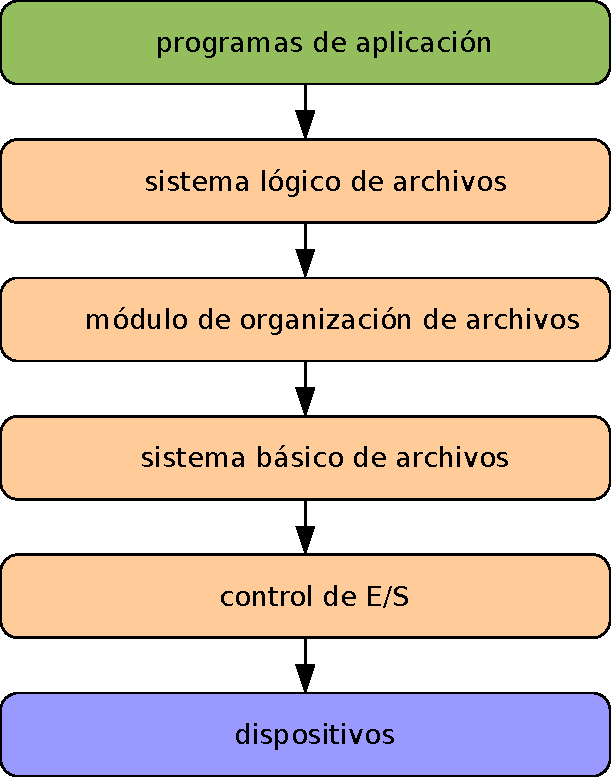
\includegraphics[width=0.8\textwidth]{media/C19_sistema_de_archivos/estructura_sistema_de_archivos.pdf}
\caption{Estructura de un sistema de
archivos.}\label{fig-estructura-sistema-de-archivos}
\end{figure}

Los sistemas de archivos son un componente complejo, por lo que suelen
estar compuesto de varios niveles diferentes. En la
\hyperref[fig-estructura-sistema-de-archivos]{Estructura de un sistema
de archivos.} se muestra un ejemplo típico de la estructura de un
sistema de archivos diseñado en niveles. Cada nivel utiliza las
funciones de los niveles inferiores y proporciona nuevas funciones a los
niveles superiores.

\subsection{Control de E/S}\label{_control_de_es}

{} En el nivel más bajo, accediendo directamente a los dispositivos de
almacenamiento, se encuentra el \textbf{control de E/S}.

Contiene los controladores de dispositivo encargados de transferir la
información entre la memoria principal y el disco. Estos controladores,
que generalmente son compartidos entre los distintos sistemas de
archivos, transfieren los datos en unidades de \textbf{bloques}{} ---en
lugar de transferir un byte cada vez--- para mejorar la eficiencia. Cada
\_*bloque* está formado por uno o más sectores.

Dependiendo de la unidad de disco, los sectores pueden tener tamaños de
entre 32 bytes y 4096 bytes. Lo más común es que su tamaño sea de 512
bytes.

\subsection{Sistema básico de
archivos}\label{_sistema_buxe1sico_de_archivos}

{} El \textbf{sistema básico de archivos} se encarga de enviar comandos
genéricos al controlador de dispositivo apropiado, con el fin de leer y
escribir bloques físicos en el disco. Cada bloque físico se identifica
mediante su dirección de disco numérica.

Por ejemplo, en dispositivos que usan direccionamiento de tipo
cabeza-cilindro-sector (CHS), la dirección de un sector podría ser:
unidad 1, cilindro 73, cabeza 2, sector 10. Mientras que en dispositivos
que admiten direccionamiento LBA (\emph{Logical Block Addressing}), la
dirección de un sector podría ser: unidad 1, sector 4691123.

El \textbf{{}LBA} es un método común para especificar la localización de
los sectores de un disco. Usa un esquema de direccionamiento lineal,
donde cada sector es identificado con un número entero único. Antes de
este método, se usaba el de cabeza-cilindro-sector (CHS), pero tenía la
desventaja de hacer públicos los detalles físicos del dispositivo de
almacenamiento.

\subsection{Módulo de organización de
archivos}\label{_muxf3dulo_de_organizaciuxf3n_de_archivos}

{} El \textbf{módulo de organización de archivos} tiene conocimiento de
los archivos y se encarga de traducir las direcciones lógicas de los
bloques en los archivos ---es decir, posición del bloque dentro del
archivo, siendo 0 la dirección del primer bloque--- en las direcciones
físicas de bloque ---por ejemplo, cilindro, cabeza y sector del bloque
correspondiente en el dispositivo de almacenamiento--- que serán
enviadas al \textbf{sistema básico de archivos} para que realice las
transferencias solicitadas.

Los bloques lógicos de cada archivo son numerados de 0 a \emph{N}, pero
los bloques físicos asignados a estos bloques lógicos no tienen por qué
coincidir en los números de bloque. Por eso, el \textbf{módulo de
organización de archivos} debe utilizar la ubicación del contenido del
archivo en el disco y la información sobre los bloques físicos
asignados, para traducir las direcciones lógicas en direcciones físicas.

Además, el módulo de organización, incluye el gestor de espacio libre,
que controla los bloques no asignados y proporciona dichos bloques
cuando el \textbf{módulo de organización de archivos} lo necesita, ya
sea para crear un archivo nuevo o para extender uno existente.

\subsection{Sistema lógico de
archivos}\label{_sistema_luxf3gico_de_archivos}

El \textbf{sistema lógico de archivos} gestiona los \textbf{metadatos}.
En los \textbf{{}metadatos} se incluye toda la estructura del sistema de
archivos, excepto los propios datos de los archivos.

Entre dichos \textbf{metadatos} está la \textbf{estructura de
directorios} y los \textbf{bloques de control de archivo}. Un
\textbf{bloque de control de archivo}{} o \textbf{{}FCB} (\emph{File
Control Block}) contiene información acerca del archivo, incluyendo su
propietario, los permisos y la ubicación del contenido del mismo.

Además, el \textbf{sistema lógico de archivos} también es responsable de
las tareas de protección y seguridad.

Cada sistema operativo puede soportar uno o más sistemas de archivos
para dispositivos de disco. Por ejemplo, en los sistemas UNIX se utiliza
el «sistema de archivos UNIX» o \{ufs\} (\emph{UNIX File System}), que
está basado en el sistema \{ffs\} (\emph{Fast File System}) de la
Universidad de Berkeley. Microsoft Windows soporta los sistemas de
archivo \{fat\} (\emph{File Allocation Table}), \{fat32\} y \{ntfs\}
(\emph{NT File System}). En Linux se soportan más de cuarenta sistemas
de archivo, entre los que cabe destacar: la familia \emph{extended
filesystem} --- \{ext2\}, \{ext3\} y \{ext4\}--- \{xfs\} y \{btrfs\}.

Además, la mayoría de los sistemas operativos modernos soportan otros
sistemas de archivo, como los utilizados en los soportes removibles. Por
ejemplo el \{iso9660\}, utilizado por la mayor parte de los CD-ROM, o el
\{udf\} (\emph{Universal Disk Format}), utilizado por los DVD-ROM y
Blu-ray.

\section{Estructuras de metadatos en
disco}\label{_estructuras_de_metadatos_en_disco}

Para implementar un sistema de archivos se utilizan diversas estructuras
de \textbf{metadatos} alojadas tanto en el disco como en la memoria.
Estas estructuras varían dependiendo del sistema operativo y del sistema
de archivos. Sin embargo, a continuación intentaremos describir
brevemente las estructuras en disco más comunes.

\subsection{Bloque de control de
arranque}\label{_bloque_de_control_de_arranque}

{} {} {} En todo sistema de archivos suele haber un \textbf{bloque de
control de arranque} ---también llamado \textbf{bloque de inicio} o
\textbf{sector de arranque}--- que suele ocupar el primer bloque de cada
volumen y que contiene la información necesaria para iniciar un sistema
operativo a partir de dicho volumen.

Este bloque puede estar vacío, si el volumen no contiene un sistema
operativo.

\subsection{Bloque de control de
volumen}\label{_bloque_de_control_de_volumen}

{} El \textbf{bloque de control de volumen} contiene todos los detalles
acerca del volumen. Por ejemplo, el número máximo de bloques, el tamaño
de los bloques, el número de bloques libres y punteros a los mismos; así
como un contador de bloques de información \textbf{FCB} ocupados y
punteros a estos.

A esta estructura se la denomina \textbf{{}superbloque}, en los sistemas
de archivos de sistemas UNIX y Linux. Mientras que en \{ntfs\} esta
información se almacena en la \textbf{tabla maestra de archivos} o
\textbf{{}MFT} (\emph{Master File Table}).

\subsection{Bloque de control de
archivo}\label{_bloque_de_control_de_archivo}

{} Todo sistema de archivos tiene un \textbf{bloque de control de
archivo} o \textbf{{}FCB} (\emph{File Control Block}) por archivo, en
que se almacenan numerosos detalles sobre cada uno de los archivos Por
ejemplo, los permisos, el propietario, el tamaño y la ubicación de los
bloques de datos, entre otros.

En términos generales, todos los \textbf{FCB} del sistema de archivos se
almacenan en una tabla denominada \textbf{directorio de dispositivo}{} o
\textbf{tabla de contenidos del volumen}{}.

En los sistemas de archivos de sistemas UNIX y Linux cada FCB se
denomina \textbf{{}inodo} y se almacenan a continuación del
\textbf{superbloque}. En \{ntfs\} esta información se almacena en la
\textbf{MFT}, ya que cada entrada de dicha tabla es un \textbf{FCB}.

\subsection{Estructura de directorios}\label{_estructura_de_directorios}

Finalmente, por lo general los sistemas de archivos tienen una
estructura de directorios, para organizar los archivos.

En los sistemas de archivos de sistemas UNIX y Linux, cada directorio es
como un archivo especial que almacena los nombres de los archivos que
contiene y los índices de los \textbf{inodos} de cada uno de ellos. En
\{ntfs\} es similar, aunque la estructura de directorios completa se
almacena en la propia \textbf{MFT}.

\section{Estructuras de metadatos en
memoria}\label{_estructuras_de_metadatos_en_memoria}

La información almacenada en memoria se utiliza tanto para la gestión
del sistema de archivos como para mejorar el rendimiento del mismo
mediante mecanismos de caché.

Los datos se cargan en el momento de comenzar a utilizar el sistema de
archivos ---proceso denominado montaje--- y se descartan cuando se va a
dejar de hacer uso del mismo ---es decir, en el desmontaje---.

Las estructuras existentes en la memoria pueden incluir las que a
continuación se describen:

\begin{itemize}
\item
  Una \textbf{tabla de montaje}{} en memoria que contiene información
  acerca de cada volumen montado en el sistema.
\item
  Una caché en memoria de la \textbf{estructura de directorios} que
  almacena la información relativa a los directorios a los que se ha
  accedido recientemente. Los directorios que actúan como puntos de
  montaje pueden contener un puntero a la entrada, en la tabla de
  montaje, del volumen montado en el directorio.
\item
  La \textbf{tabla global de archivos abiertos}{} que contiene una copia
  del \textbf{FCB} de cada archivo abierto en el sistema, además de
  otras informaciones.
\item
  La \textbf{tabla de archivos abiertos}{} de cada proceso. El
  \textbf{PCB} de cada proceso contiene una tabla donde se listan los
  archivos abiertos por el proceso.
\end{itemize}

La \textbf{tabla de archivos abiertos} contiene, para cada archivo, un
puntero a la entrada correspondiente del mismo archivo en la tabla
global de archivos abiertos, pero también guarda otras informaciones
adicionales que son particulares de cada proceso. Por ejemplo, si el
proceso lo ha abierto para lectura o escritura o la posición del puntero
que indica la siguiente posición a leer o escribir.

\section{Montaje de sistemas de
archivos}\label{_montaje_de_sistemas_de_archivos}

{} Un sistema de archivos debe \textbf{montarse} para que sus archivos
sean accesibles a los procesos del sistema. El proceso de montaje
incluye los siguientes pasos:

\begin{enumerate}
\def\labelenumi{\arabic{enumi}.}
\item
  Al sistema operativo se le debe proporcionar el nombre o identificador
  del dispositivo y el punto de montaje. El \textbf{punto de montaje}{}
  es la ubicación dentro de la estructura de directorios ---la ruta al
  directorio concreto--- a la que queremos conectar el sistema de
  archivos. Después de que el proceso de montaje se haya completado, los
  archivos y directorios del sistema de archivos montado serán
  accesibles como descendientes del directorio del \textbf{punto de
  montaje}.
\item
  A continuación el sistema operativo verifica que el dispositivo
  contiene un sistema de archivos válido. Para ello lee el
  \textbf{bloque de control de volumen} y comprueba que tiene un formato
  válido.
\item
  Finalmente el sistema operativo registra en la \textbf{tabla de
  montaje} el tipo de sistema de archivos y el identificador del
  dispositivo montado. Después, almacena el índice de la entrada
  correspondiente en la \textbf{tabla de montaje} en la copia en memoria
  del \textbf{FCB} del directorio que hace de \textbf{punto de montaje}.

  Esto permite que pueda ser recorrida la estructura de directorios de
  distintos sistemas de archivos, pasando de uno a otro de forma
  transparente, según sea necesario.
\end{enumerate}

En muchos sistemas operativos modernos, el montaje se ejecuta
automáticamente cuando los dispositivos son detectados durante el
arranque del sistema o cuando se conectan durante el funcionamiento del
mismo ---por ejemplo, cuando se inserta un medio en la unidad CD-ROM o
se pincha una memoria flash en un puerto USB---. En algunos se permite,
además, que el administrador del equipo ejecute operaciones de montaje
manuales.

\section{Archivos}\label{_archivos}

Cada sistema de archivos almacena en disco una tabla donde cada entrada
guarda un \textbf{bloque de control de archivo} o \textbf{FCB}
(\emph{File Control Block}) por archivo. Concretamente, en cada
\textbf{FCB} se almacena diversa información acerca del archivo al que
representa.

\subsection{Atributos de archivos}\label{_atributos_de_archivos}

La colección de atributos asociada a un archivo varía de un sistema
operativo a otro, pero típicamente son los siguientes:

\begin{itemize}
\item
  \textbf{Nombre}. Nombre simbólico del archivo, que se mantiene en un
  formato legible por la conveniencia de los usuarios.
\item
  \textbf{Identificador}. Identifica de forma unívoca el archivo dentro
  del sistema de archivos. Generalmente es el índice del \textbf{FCB} en
  la \textbf{tabla de contenidos del volumen}, donde se almacenan los
  \textbf{FCB}.
\item
  \textbf{Tipo}. Es un atributo necesario en los sistemas que soportan
  diferentes tipos de archivos.
\item
  \textbf{Ubicación}. Es un puntero a un dispositivo y a la ubicación de
  los bloques con los datos del archivo dentro del mismo.
\item
  \textbf{Tamaño}. Indica el tamaño actual de archivo ---en bytes,
  palabras o bloques--- y, posiblemente, el tamaño máximo permitido.
\item
  \textbf{Protección}. Información de control de acceso que determina
  quién puede leerlo, escribirlo, ejecutarlo, etc.
\item
  \textbf{Fecha, hora e identificación del usuario}. Esta información
  puede mantenerse para los sucesos de creación, de última modificación
  y último uso del archivo. Puede resultar útil para la protección,
  seguridad y monitorización del uso del archivo.
\end{itemize}

Los atributos de los archivos se almacenan en las estructuras de
\textbf{metadatos}.

Normalmente el nombre se almacena en la estructura de directorios, de
tal manera que una entrada de directorio está compuesta del nombre de un
archivo y del identificador de su \textbf{FCB}. Dicho identificador
permite localizar el \textbf{FCB} en la \textbf{tabla de contenidos del
volumen}, que contiene el resto de los atributos del archivo.

En \{file\_attribs\_cpp\} se muestra como leer algunos atributos de un
archivo utilizando la función \{linux\_stat\} de los sistemas POSIX.
Esta función recibe la ruta de un archivo o directorio y devuelve una
estructura de tipo \texttt{stat} con sus atributos.

\begin{Shaded}
\begin{Highlighting}[]
\KeywordTok{struct}\NormalTok{ stat}
\OperatorTok{\{}
\NormalTok{    dev\_t     st\_dev}\OperatorTok{;}         
\NormalTok{    ino\_t     st\_ino}\OperatorTok{;}         
\NormalTok{    mode\_t    st\_mode}\OperatorTok{;}        
\NormalTok{    nlink\_t   st\_nlink}\OperatorTok{;}       
\NormalTok{    uid\_t     st\_uid}\OperatorTok{;}         
\NormalTok{    gid\_t     st\_gid}\OperatorTok{;}         
\NormalTok{    dev\_t     st\_rdev}\OperatorTok{;}        
\NormalTok{    off\_t     st\_size}\OperatorTok{;}        
\NormalTok{    blksize\_t st\_blksize}\OperatorTok{;}     
\NormalTok{    blkcnt\_t  st\_blocks}\OperatorTok{;}      
    \KeywordTok{struct}\NormalTok{ timespec  st\_atim}\OperatorTok{;} 
    \KeywordTok{struct}\NormalTok{ timespec  st\_mtim}\OperatorTok{;} 
    \KeywordTok{struct}\NormalTok{ timespec  st\_ctim}\OperatorTok{;} 
\OperatorTok{\};}
\end{Highlighting}
\end{Shaded}

\begin{itemize}
\item
  Identificador del dispositivo donde se almacena el archivo.
\item
  Número de inodo del archivo.
\item
  Permisos y tipo de archivo.
\item
  Número de enlaces duros al archivo.
\item
  Identificador del usuario propietario del archivo.
\item
  Identificador del grupo propietario del archivo.
\item
  Identificador del dispositivo si el archivo corresponde a un
  dispositivo.
\item
  Tamaño del archivo en bytes.
\item
  Tamaño de bloque recomendado para hacer operaciones de E/S.
\item
  Número de bloques de 512 bytes asignados al archivo en el
  almacenamiento.
\item
  Fecha y hora del último acceso al archivo.
\item
  Fecha y hora de la última modificación del archivo.
\item
  Fecha y hora del último cambio de metadatos del archivo.
\end{itemize}

\subsection{Operaciones con los
archivos}\label{_operaciones_con_los_archivos}

Un archivo es un tipo abstracto de datos sobre el que pueden realizarse
diversas operaciones. Concretamente el sistema operativo proporciona
llamadas al sistema para: crear, abrir, escribir, leer, reposicionar el
puntero de lectura/escritura, borrar y truncar o redimensionar archivos.

Generalmente el sistema mantiene un puntero de lectura/escritura que
hace referencia a la ubicación dentro del archivo en la que debe tener
lugar la siguiente operación. Este puntero se actualiza, avanzando cada
vez que se realiza una nueva lectura/escritura.

Para desplazarse aleatoriamente por el archivo, el sistema operativo
debe ofrecer una llamada al sistema que permita reposicionar el puntero
allí donde interese.

Muchos sistemas también disponen de operaciones para consultar y
modificar diversos atributos de un archivo, como la longitud o el
propietario del mismo. Además, se suelen incluir llamadas para otras
operaciones comunes, como añadir datos al final de un archivo o el
renombrado de un archivo existente.

\begin{longtable}[]{@{}
  >{\raggedright\arraybackslash}p{(\linewidth - 4\tabcolsep) * \real{0.3333}}
  >{\raggedright\arraybackslash}p{(\linewidth - 4\tabcolsep) * \real{0.3333}}
  >{\raggedright\arraybackslash}p{(\linewidth - 4\tabcolsep) * \real{0.3333}}@{}}
\caption{Funciones de la API para manipular archivos.}\tabularnewline
\toprule\noalign{}
\begin{minipage}[b]{\linewidth}\raggedright
\end{minipage} & \begin{minipage}[b]{\linewidth}\raggedright
POSIX API
\end{minipage} & \begin{minipage}[b]{\linewidth}\raggedright
Windows API
\end{minipage} \\
\midrule\noalign{}
\endfirsthead
\toprule\noalign{}
\begin{minipage}[b]{\linewidth}\raggedright
\end{minipage} & \begin{minipage}[b]{\linewidth}\raggedright
POSIX API
\end{minipage} & \begin{minipage}[b]{\linewidth}\raggedright
Windows API
\end{minipage} \\
\midrule\noalign{}
\endhead
\bottomrule\noalign{}
\endlastfoot
\textbf{Crear archivos} & \{linux\_open\} / \{linux\_openat\} &
\{win32\_createfile\} \\
\textbf{Abrir archivos} & \{linux\_open\} / \{linux\_openat\} &
\{win32\_openfile\} \\
\textbf{Cerrar archivos} & \{linux\_close\} & \{win32\_closehandle\} \\
\textbf{Borrar archivos} & \{linux\_unlink\} & \{win32\_deletefile\} \\
\textbf{Leer contenidos} & \{linux\_read\} & \{win32\_readfile\} \\
\textbf{Escribir contenido} & \{linux\_write\} & \{win32\_writefile\} \\
\textbf{Reposicionar puntero de lectura/escritura} & \{linux\_lseek\} &
\{win32\_setfilepointer\} \\
\textbf{Redimensionar archivos} & \{linux\_ftruncate\} &
\{win32\_setendoffile\} \\
\textbf{Consultar atributos} & \{linux\_stat\} / \{linux\_fstat\} &
\{win32\_getfileattributes\} \\
\textbf{Renombrar archivos} & \{linux\_rename\} & \{win32\_movefile\} \\
\textbf{Copiar archivos} & & \{win32\_movefile\} \\
\textbf{Mover archivos} & \{linux\_rename\} {solo en el mismo sistema de
archivos} & \{win32\_copyfile\} \\
\end{longtable}

Estas operaciones primitivas pueden combinarse, a su vez, para realizar
otras operaciones más complejas ---por ejemplo, crear una copia de un
archivo o moverlo a otro lugar de la estructura de directorios---.

\subsection{Abrir archivos}\label{_abrir_archivos}

La mayor parte de las operaciones comentadas implican realizar una
búsqueda en el directorio para encontrar la entrada asociada con el
archivo cuyo nombre se ha indicado. Para evitar realizar esta búsqueda
una y otra vez, muchos sistemas requieren que el proceso haga una
llamada al sistema \textbf{open}, antes de realizar cualquiera de estas
operaciones por primera vez sobre un archivo.

En unos pocos sistemas, los archivos se abren automáticamente cuando un
proceso solicita su primera operación sobre los mismos y se cierran
cuando el proceso termina. Sin embargo, lo más común es que los procesos
tengan que abrir los archivos explícitamente.

En concreto la operación \textbf{open}:

\begin{enumerate}
\def\labelenumi{\arabic{enumi}.}
\item
  Busca en el directorio el nombre del archivo, hasta encontrar la
  entrada asociada y recupera el identificador del mismo.
\item
  Utiliza el identificador del archivo para recuperar el \textbf{FCB}
  correspondiente.
\item
  Crea una entrada para el archivo en la \textbf{tabla de archivos
  abiertos} donde se almacena la información del FCB.
\item
  Retorna al proceso devolviendo un identificador ---en forma de puntero
  o de índice--- a la nueva entrada en la tabla de archivos abiertos.
\end{enumerate}

El nombre con el que se designa a esas entradas en la tabla de archivos
abiertos varía de unos sistemas operativos a otros. En los sistemas
POSIX se utiliza el término \textbf{{}descriptor de archivo} ---o
\textbf{\emph{file descriptor}}--- mientras que en los sistemas
Microsoft Windows se prefiere el término \textbf{manejador de archivo}{}
---o \textbf{\emph{file handler}}---. Por ejemplo, en el
\hyperref[ejemplo-archivos]{example\_title} se ilustra cómo se usa la
función \{linux\_open\} para abrir un archivo, obteniendo un
\textbf{descriptor de archivo} de tipo \texttt{int} que luego se usa
para leer su contenido y copiarlo en un archivo diferente.

Después de utilizar la llamada al sistema \textbf{open}, cuando se desea
solicitar una operación sobre un archivo, solo es necesario proporcionar
el identificador devuelto, evitando así que haga falta realizar
nuevamente la exploración del directorio para buscar el archivo. Por
ejemplo, en el \hyperref[ejemplo-archivos]{example\_title} el
\textbf{descriptor de archivo} devuelto por \{linux\_open\} se utiliza
en las llamadas a \{linux\_read\} y \{linux\_write\}, para leer y
escribir el contenido del archivo.

En este ejemplo se muestra cómo abrir un archivo, leer su contenido y
escribirlo en otro archivo en sistemas POSIX. Como el archivo el de
origen puede tener cualquier tamaño, se lee en bloques de tamaño
\texttt{BUFSIZ} y se escribe en el archivo de destino en bloques del
mismo tamaño, en lugar de intentar leer el contenido completo de una
sola vez.

El código fuente completo de este ejemplo está disponible en
\{file\_copy\_cpp\}.

\begin{Shaded}
\begin{Highlighting}[]
\DataTypeTok{int}\NormalTok{ source\_fd }\OperatorTok{=}\NormalTok{ open}\OperatorTok{(} \StringTok{"foo.txt"}\OperatorTok{,}\NormalTok{ O\_RDONLY }\OperatorTok{);}  
\ControlFlowTok{if} \OperatorTok{(}\NormalTok{source\_fd }\OperatorTok{==} \OperatorTok{{-}}\DecValTok{1}\OperatorTok{)} 
\OperatorTok{\{}
    \CommentTok{// Aquí va el código para usar el error de open()...}
\OperatorTok{\}}

\CommentTok{// ...}

\DataTypeTok{int}\NormalTok{ dest\_fd }\OperatorTok{=}\NormalTok{ open}\OperatorTok{(} \StringTok{"bar.txt"}\OperatorTok{,}\NormalTok{ O\_WRONLY }\OperatorTok{|}\NormalTok{ O\_CREAT }\OperatorTok{|}\NormalTok{ O\_TRUNC}\OperatorTok{,} \BaseNTok{0666} \OperatorTok{);} 
\ControlFlowTok{if} \OperatorTok{(}\NormalTok{dest\_fd }\OperatorTok{==} \OperatorTok{{-}}\DecValTok{1}\OperatorTok{)}
\OperatorTok{\{}
    \CommentTok{// Aquí va el código para usar el error de open()...}
\OperatorTok{\}}

\DataTypeTok{char}\NormalTok{ buffer}\OperatorTok{[}\NormalTok{BUFSIZ}\OperatorTok{];}
\DataTypeTok{ssize\_t}\NormalTok{ bytes\_read}\OperatorTok{;}
\ControlFlowTok{while} \OperatorTok{((}\NormalTok{bytes\_read }\OperatorTok{=}\NormalTok{ read}\OperatorTok{(}\NormalTok{ source\_fd}\OperatorTok{,}\NormalTok{ buffer}\OperatorTok{,} \KeywordTok{sizeof}\OperatorTok{(}\NormalTok{buffer}\OperatorTok{)} \OperatorTok{))} \OperatorTok{\textgreater{}} \DecValTok{0}\OperatorTok{)}  
\OperatorTok{\{}
    \ControlFlowTok{if} \OperatorTok{(}\NormalTok{write}\OperatorTok{(}\NormalTok{ dest\_fd}\OperatorTok{,}\NormalTok{ buffer}\OperatorTok{,}\NormalTok{ bytes\_read }\OperatorTok{)} \OperatorTok{==} \OperatorTok{{-}}\DecValTok{1}\OperatorTok{)}  
    \OperatorTok{\{}
        \CommentTok{// Aquí va el código para usar el error de write()...}
    \OperatorTok{\}}
\OperatorTok{\}}

\ControlFlowTok{if} \OperatorTok{(}\NormalTok{bytes\_read }\OperatorTok{==} \OperatorTok{{-}}\DecValTok{1}\OperatorTok{)} 
\OperatorTok{\{}
    \CommentTok{// Aquí va el código para usar el error de read()...}
\OperatorTok{\}}

\NormalTok{close}\OperatorTok{(}\NormalTok{ source\_fd }\OperatorTok{);} 
\NormalTok{close}\OperatorTok{(}\NormalTok{ dest\_fd }\OperatorTok{);} 
\end{Highlighting}
\end{Shaded}

\begin{itemize}
\item
  Abrir el archivo \texttt{foo.txt} en modo lectura (opción
  \texttt{O\_RDONLY}).
\item
  En caso de éxito, la función \{linux\_open\} devuelve un
  \textbf{descriptor de archivo} que se guarda en \texttt{source\_fd}.
  Si el valor devuelto es negativo, indica que ha ocurrido un error al
  abrir el archivo.
\item
  Abrir el archivo \texttt{bar.txt} en modo escritura (opción
  \texttt{O\_WRONLY}), creándolo si no existe (opción \texttt{O\_CREAT})
  y truncando su tamaño a 0 si ya existe (opción \texttt{O\_TRUNC}).

  En caso de crear el archivo, se usarán los permisos de lectura y
  escritura para todos (\texttt{0666}) en función de la
  \textbf{\emph{umask}} del proceso (véase el
  \hyperref[acl_condensada]{Lista de control de acceso condensada})
\item
  Leer el contenido del archivo \texttt{foo.txt} en bloques de tamaño
  \texttt{BUFSIZ} y almacenarlo en el búfer \texttt{buffer}. La función
  \{linux\_read\} devuelve el número de bytes leídos, que puede ser
  menos que la cantidad solicitada \texttt{BUFSIZ} si se ha llegado al
  final del archivo.
\item
  La función \{linux\_read\} devuelve el número de bytes leídos o
  \texttt{-1} si ha ocurrido un error.
\item
  Escribir \texttt{bytes\_read} bytes de contenido del búfer
  \texttt{buffer} en el archivo \texttt{bar.txt}. Se utiliza el valor de
  la variable \texttt{bytes\_read} devuelto por \{linux\_read\} para
  escribir con la función \{linux\_write\} la misma cantidad de bytes
  que fue leída en la llamada previa a \{linux\_read\}.
\item
  La función \{linux\_write\} devuelve el número de bytes escritos o
  \texttt{-1} si ha ocurrido un error.
\item
  Cerrar los archivos \texttt{foo.txt} y \texttt{bar.txt} con la función
  \{linux\_close\}. Esto libera los recursos asociados a los archivos
  abiertos y actualiza la tabla de archivos abiertos del proceso.
\end{itemize}

En sistemas operativos donde varios procesos pueden abrir un mismo
archivo, se suelen utilizar dos niveles de tablas de archivos abiertos:

\begin{enumerate}
\def\labelenumi{\arabic{enumi}.}
\item
  Una \textbf{tabla para cada proceso} ---almacenada en el
  \textbf{PCB}--- donde se indican todos los archivos que el proceso
  tiene abiertos.

  En dicha tabla se almacena toda la información referente al uso de
  cada archivo por parte de un proceso. Por ejemplo, se puede almacenar
  la posición actual utilizada por las operaciones de lectura y
  escritura o los derechos de acceso.
\item
  Una \textbf{tabla global para todo el sistema} donde se almacena toda
  la información independiente de los procesos, como la ubicación del
  archivo en el disco, las fechas de acceso y el tamaño del archivo.
\end{enumerate}

Cuando un proceso invoca la llamada \textbf{open}, se añade una entrada
en la \textbf{tabla de archivos abiertos del proceso}, que a su vez
apunta a la entrada correspondiente dentro de la \textbf{tabla global
del sistema}. Si el archivo no existe en esta última, también hay que
crear una entrada en la tabla global del sistema haciendo uso de la
información contenida en disco en el \textbf{FCB} correspondiente.

Es muy común, que la \textbf{tabla global} almacene un \textbf{contador
de aperturas} para cada archivo, con el objetivo de indicar cuántos
procesos lo mantienen abierto.

Cuando el archivo deja de ser utilizado activamente por el proceso,
puede ser cerrado utilizando la llamada al sistema \textbf{close}.
Entonces el \textbf{contador de aperturas} se decrementa, de forma que
cuando alcance cero querrá decir que la entrada puede ser eliminada de
la \textbf{tabla global de archivos abiertos}.

\subsection{Tipos de archivo}\label{_tipos_de_archivo}

Cuando se diseña un sistema operativo es necesario considerar si debe
reconocer y soportar el concepto de \textbf{tipo de archivo}. Si el
sistema operativo reconoce el \textbf{tipo de un archivo} puede operar
con el mismo de formas razonables. Por ejemplo, el sistema puede impedir
que un usuario intente imprimir los archivos que contienen programas en
formato binario, pues el documento impreso sería ininteligible.

En los sistemas operativos más comunes las técnicas utilizadas para
implementar los tipos de archivo son las siguientes:

\begin{itemize}
\item
  En MS-DOS y Microsoft Windows el tipo de archivo se incluye como parte
  del nombre del archivo. Es decir, el nombre se divide en dos partes:
  un nombre y una extensión, separadas por un punto.

  El sistema puede utilizar la extensión para conocer el tipo de archivo
  y el tipo de operaciones que se pueden realizar con el mismo.
\item
  En macOS cada archivo tiene un atributo que almacena el tipo ---por
  ejemplo, TEXT para los archivos de texto o APPL para las
  aplicaciones--- y otro que contiene el nombre del programa que lo
  creó. Cuando el usuario hace clic con el ratón sobre el icono de un
  archivo, el programa que lo creó se ejecuta automáticamente y este
  abre el archivo.
\item
  En los sistemas estilo UNIX se utiliza un \textbf{número mágico},
  almacenado al principio de algunos archivos, para indicar el tipo del
  mismo. No todos los archivos tienen números mágicos, por lo que se
  permite hacer sugerencias en forma de extensiones del nombre del
  archivo.

  Sin embargo, en estos sistemas estas extensiones no son obligatorias
  ni el sistema depende de ellas. Su objetivo, fundamentalmente, es
  ayudar a los usuarios a determinar el tipo de contenido de un archivo,
  por lo que pueden ser utilizadas o ignoradas por cada aplicación
  concreta, en función de las preferencias de sus desarrolladores.
\end{itemize}

En los sistemas estilo UNIX es muy útil el comando \texttt{file} que
permite determinar el tipo de un archivo a partir de su contenido,
utilizando un conjunto de reglas y una base de datos de \textbf{números
mágicos}.

\section{Estructura de directorios}\label{_estructura_de_directorios_2}

Algunos sistemas de archivos pueden almacenar millones de archivos en
terabytes de disco. Para gestionar todos esos datos necesitamos
organizarlos de alguna manera, lo que generalmente implica el uso de
directorios.

Un \textbf{{}directorio} puede considerarse una tabla de símbolos que
traduce los nombre de los archivos en los identificadores que permiten
recuperar sus correspondientes entradas en la \textbf{tabla de
contenidos del volumen}, donde se almacenan los \textbf{FCB}.

En los sistemas POSIX, los directorios se crean llamando a
\{linux\_mkdir\} y se eliminan con \{linux\_rmdir\}. Mientras que en
Microsoft Windows se crean con \{win32\_createdirectory\} y se eliminan
con \{win32\_removedirectory\}.

Por otro lado, en \{dir\_list\_cpp\} se muestra cómo un programa puede
acceder al contenido de un directorio, utilizando las funciones
\{linux\_opendir\} y \{linux\_readdir\} de la librería de los sistemas
POSIX.

A continuación vamos a estudiar los diversos esquemas para definir la
estructura lógica del sistema de directorios.

\subsection{Directorios de un nivel}\label{_directorios_de_un_nivel}

En la estructura de directorios de un nivel todos los archivos están
contenidos en un único directorio.

Esto presenta algunas limitaciones:

\begin{itemize}
\item
  Cuando el número de usuarios del sistema aumenta se hace más difícil
  que cada uno escoja nombres diferentes para sus archivos. Esto es
  necesario, puesto que todos los archivos se encuentran en el mismo
  directorio.
\item
  Incluso en los sistemas operativos monousuario, puede ser difícil para
  un usuario mantener organizados sus datos a medida que se incrementa
  el número de archivos.
\end{itemize}

Este esquema fue utilizado por la primera versión del sistema operativo
MS-DOS.

\subsection{Directorio de dos niveles}\label{_directorio_de_dos_niveles}

En la estructura de directorios de dos niveles cada usuario tiene su
propio \textbf{directorio de archivos de usuario}{} o \textbf{{}UFD}
(\emph{User File Directory}) que cuelga del \textbf{directorio maestro
de archivos}{} o \textbf{{}MFD} (\emph{Master File Directory}).

Cuando un usuario se conecta al sistema o inicia un trabajo, se explora
el \textbf{MFD}. Esta es una tabla indexada por el nombre de los
usuarios o por los números de cuenta, donde cada una de sus entradas
apunta al \textbf{UFD} de dicho usuario. Puesto que cada \textbf{UFD}
incluye solo los archivos del usuario al que pertenece, el sistema
operativo puede confinar todas las operaciones que puede realizar un
usuario sobre los archivos a su \textbf{UFD}.

Aunque esto resuelve el problema de la colisión de nombres entre
diferentes usuarios, también presenta algunas desventajas:

\begin{itemize}
\item
  La estructura descrita aísla a los usuarios, lo cual puede ser un
  problema cuando estos quieren compartir datos para cooperar en alguna
  tarea.

  La solución pasa por utilizar \textbf{nombres de ruta}{} para designar
  a un archivo de forma unívoca. Por ejemplo, si el usuario
  \texttt{usera} quiere acceder a su archivo \texttt{test}, simplemente
  debe referirse a él como \texttt{test}. Mientras que si quiere acceder
  al archivo \texttt{test} del usuario \texttt{userb}, debe utilizar un
  \textbf{nombre de ruta} como \texttt{/userb/test}, donde se indica el
  nombre del usuario y el nombre del archivo.

  En general, cada sistema operativo utiliza su propia sintaxis para
  nombrar los archivos contenidos en los directorios de otros usuarios.
\item
  Puede ser difícil para un usuario mantener organizados sus datos a
  medida que se incrementa el número de archivos personales, incluso
  aunque tenga un directorio para él solo.
\end{itemize}

\subsection{Directorios con estructura de
árbol}\label{_directorios_con_estructura_de_uxe1rbol}

La estructura de directorio de dos niveles puede generalizarse en la
\textbf{estructura de directorios en árbol} de altura arbitraria. Esto
permite que los usuarios puedan crear sus propios subdirectorios para
organizar sus archivos de la forma más conveniente.

Cada sistema de archivos tiene un \textbf{directorio raíz}{} que puede
contener tanto archivos como otros directorios. A su vez, cada
directorio puede contener un conjunto de archivos y subdirectorios.

Normalmente, cada entrada de directorio incluye un bit donde se indica
si dicha entrada apunta a un archivo o a un subdirectorio. Esto se hace
así porque, generalmente, los directorios no son más que archivos con un
formato interno especial; por lo que el sistema debe saber si la entrada
apunta a un directorio para interpretar correctamente los datos del
directorio.

\subsubsection{Directorio de trabajo
actual}\label{_directorio_de_trabajo_actual}

{} Comúnmente, en el \textbf{PCB} de cada proceso se guarda cuál es su
\textbf{directorio de trabajo} actual. De esta forma, cuando se hace
referencia a un archivo en una llamada al sistema usando solo su nombre,
se le busca en el \textbf{directorio de trabajo} del proceso.

Si se necesita un archivo que no se encuentra en el \textbf{directorio
de trabajo} actual, entonces el usuario debe especificar un
\textbf{nombre de ruta} desde el \textbf{directorio de trabajo}, o
primero cambiar con una llamada al sistema el directorio de trabajo del
proceso al directorio donde está almacenado el archivo.

Windows API permite indicar el \textbf{directorio de trabajo} de un
nuevo proceso al crearlo, a través del argumento
\texttt{lpCurrentDirectory} de \{win32\_createprocess\}. Si este
argumento vale NULL, el proceso hereda el \textbf{directorio de trabajo}
del padre. En todo caso, cualquier proceso puede cambiar su
\textbf{directorio de trabajo} actual llamando a
\{win32\_setcurrentdirectory\}.

En los sistemas POSIX, el proceso hijo creado con \{linux\_fork\} hereda
automáticamente el \textbf{directorio de trabajo} actual del proceso
padre. Por lo que si necesitamos cambiar su \textbf{directorio de
trabajo} ---por ejemplo, antes de llamar a \{linux\_exec\} para cambiar
el \textbf{directorio de trabajo} para el nuevo programa--- el proceso
puede usar \{linux\_chdir\}.

Gracias a la herencia del \textbf{directorio de trabajo} es como los
\textbf{intérpretes de comandos} indican a los comandos que ejecutan en
qué directorio deben ejecutarse.

Por ejemplo, en los sistemas POSIX el intérprete de comandos
\textbf{Bash} se inicia usando el directorio personal del usuario como
\textbf{directorio de trabajo}. El usuario puede cambiar el
\textbf{directorio de trabajo} del proceso de la \textbf{Bash} usando el
comando interno \texttt{cd}. Cuando se pide a la \textbf{Bash} que
ejecute cualquier otro comando, esta crea un nuevo proceso hijo donde
ejecutar el programa de dicho comando. Ese proceso hereda el
\textbf{directorio de trabajo} actual de \textbf{Bash}.

\subsubsection{Nombre de ruta}\label{_nombre_de_ruta}

{} Los \textbf{nombres de ruta} es la forma en la que se indica la
ubicación de un archivo o directorio en el árbol de directorios.

Los \textbf{nombres de ruta} pueden ser de dos tipos:

\begin{itemize}
\item
  Un \textbf{nombre de ruta absoluto}{} comienza en la raíz y va
  indicando los directorios que componen la ruta de forma descendente
  hasta llegar al archivo especificado.

  Por ejemplo, \texttt{/usr/share/doc},
  \texttt{C:\textbackslash{}Program\ Files\textbackslash{}WindowsApps} o
  \texttt{\textbackslash{}Windows\textbackslash{}System32}
\item
  Un \textbf{nombre de ruta relativo}{} define una ruta a partir del
  \textbf{directorio de trabajo actual}.

  Por ejemplo, \texttt{Imágenes/Enero/000001.jpg},
  \texttt{Downloads\textbackslash{}horario.zip} o
  \texttt{C:Desktop\textbackslash{}Proyectos}.
\end{itemize}

Con una \textbf{estructura de directorios en árbol}, unos usuarios
pueden acceder a los archivos de otros. Para eso, solo es necesario que
se utilicen \textbf{nombres de ruta} para designar los archivos del otro
usuario, o que se cambie el \textbf{directorio de trabajo actual}.

Este tipo de estructura de directorios es la utilizada por MS-DOS y por
las distintas versiones de Microsoft Windows.

\subsection{Directorios en grafo
acíclico}\label{_directorios_en_grafo_acuxedclico}

La \textbf{estructura de directorio en grafo acíclico} es una
generalización natural del esquema con \textbf{estructura en árbol}.

A diferencia de este último, la \textbf{estructura en grafo acíclico}
permite que los mismos archivos y subdirectorios existan simultáneamente
en distintos lugares de la estructura de directorios. Eso significa que
para acceder a un archivo o directorio pueden existir diversos
\textbf{nombres de ruta}.

Esto, por ejemplo, permite que los usuarios puedan compartir archivos de
tal forma que los mismos archivos y directorios estén disponibles
directamente desde el directorio personal de los diferentes usuarios.

\subsubsection{Enlaces}\label{_enlaces}

Los archivos y subdirectorios compartidos pueden implementarse de
diversas formas:

\begin{itemize}
\item
  Se puede crear una entrada de directorio especial denominada
  \textbf{{}enlace}. Un \textbf{enlace} es, generalmente, un archivo que
  contiene la ruta relativa o absoluta de otro archivo o subdirectorio.
  En los sistemas POSIX a estos se los conoce como \textbf{enlaces
  simbólicos}{}.
\item
  También se puede duplicar toda la información de la entrada de
  directorio del archivo compartido en todos los directorios que también
  contienen dicho archivo.

  Así, mientras que los \textbf{enlaces simbólicos} son claramente
  diferentes de la entrada original de directorio, las entradas de
  directorio duplicadas hacen que la entrada original y la copia sean
  indistinguibles. En los sistemas POSIX, a este tipo de entradas
  duplicadas se las conoce como \textbf{enlaces duros}{}.
\end{itemize}

Como \textbf{enlaces simbólicos} almacenan una ruta, pueden apuntar a
archivos o directorios en otros sistemas de archivos. Mientras que los
\textbf{enlaces duros} solo pueden apuntar a archivos en el mismo
sistema de archivos.

En los sistemas POSIX los \textbf{enlaces duros} se crean llamando a
\{linux\_link\} y los \textbf{enlaces simbólicos} con
\{linux\_symlink\}.

En Microsoft Windows se soportan ambos tipos de enlaces desde la primera
versión ---Microsoft Windows NT 3.1--- pero únicamente en el sistema de
archivos \{ntfs\} y solo por compatibilidad con las aplicaciones POSIX.
Windows API no tuvo funciones para crear \textbf{enlaces} hasta mucho
después. Por eso su uso en Microsoft Windows no es tan común.

En Windows API los \textbf{enlaces duros} se crean con
\{win32\_createhardlink\} desde Windows 2000. Mientras que los
\textbf{enlaces simbólicos} se crean con \{win32\_createsymboliclink\}
desde Windows Vista.

\subsubsection{Inconvenientes}\label{_inconvenientes}

Una estructura en grafo acíclico es más flexible que una estructura en
árbol, pero no por eso está exenta de inconvenientes:

\begin{itemize}
\item
  Si estamos intentando recorrer el sistema de archivos completo ---por
  ejemplo, para buscar un archivo o para copiarlos en un dispositivo
  para hacer copias de seguridad--- debemos evitar acceder más de una
  vez a los archivos y subdirectorios enlazados. No olvidemos que en los
  sistemas con estructura en grafo acíclico, cada archivo puede tener
  múltiples nombres de ruta absoluta.

  Esto es más sencillo de resolver en el caso de los \textbf{enlaces
  simbólicos}, puesto que podemos evitar recorrerlos al ser claramente
  distinguibles de los archivos normales.
\item
  Los diseñadores deben enfrentarse a la cuestión de cuándo liberar el
  espacio asignado a un archivo enlazado. Si lo hacemos cuando un
  usuario lo borra podríamos dejar \textbf{enlaces} que referencian a
  archivos que no existen.
\end{itemize}

Sobre esta última cuestión:

\begin{itemize}
\item
  El caso más sencillo de resolver es el de los \textbf{enlaces
  simbólicos}, ya que pueden ser borrados sin que el archivo original se
  vea afectado, puesto que lo que se elimina es el \textbf{enlace} y no
  el archivo original.
\item
  Si lo que se pretende borrar es la entrada de un archivo original que
  es apuntado desde un \textbf{enlace simbólico}, tampoco hay problema
  en hacerlo y liberar el espacio asignado al mismo, dejando que el
  enlace apunte a un archivo que no existe. Cuando se produzca un
  intento de acceder a los archivos a través del \textbf{enlace}, el
  sistema determinará que el archivo referenciado fue borrado y tratará
  el acceso al enlace de forma similar a cualquier otro acceso ilegal a
  un archivo que no existe.
\end{itemize}

Ciertamente, podríamos plantearnos la posibilidad de buscar todos los
\textbf{enlaces} al archivo borrado y eliminarlos. Pero, a menos que el
FCB de cada archivo guarde las rutas a los \textbf{enlaces} que le
señalan, esta búsqueda podría ser muy costosa.

\begin{itemize}
\item
  Otra opción es almacenar en la entrada del archivo original un
  contador con el número de referencias al archivo. Cada vez que se
  elimina una referencia se decrementa el contador. Cuando el contador
  sea 0, sabremos que ha llegado el momento de liberar el espacio
  asignado.

  En los sistemas UNIX se utiliza esta técnica para saber cuándo liberar
  el contenido de archivos con \textbf{enlaces duros}.
\end{itemize}

Por último, no debemos olvidar que la estructura de directorios en grafo
se conserva acíclica si se prohíbe que haya múltiples referencias a un
mismo directorio. Ese es el motivo por el que en muchos sistemas POSIX
no se permite, por defecto, que los \textbf{enlaces duros} hagan
referencia a directorios. Sin embargo si se pueden utilizar
\textbf{enlaces simbólicos} para este fin, puesto que al ser
distinguibles del directorio original podemos evitar los ciclos, si
mientras se explora se ignoran dichos enlaces.

\subsection{Directorios en forma de grafo
general}\label{_directorios_en_forma_de_grafo_general}

Uno de los principales problemas de la \textbf{estructura de directorios
en grafo acíclico} es garantizar que no exista ningún ciclo. Esto es
interesante, puesto que mientras sea así los algoritmos diseñados para
recorrer el grafo y para determinar cuándo no existen más referencias a
un archivo, son relativamente simples.

No olvidemos que:

\begin{itemize}
\item
  Es importante evitar encontrar cualquier archivo dos o más veces,
  tanto por razones de corrección como de rendimiento.
\item
  En una \textbf{estructura de directorios en forma de grafo general}
  que use contadores de referencia para borrar archivos cuando no hay
  más referencias, puede que dicho contador no sea 0, aunque no haya más
  referencias al archivo.
\end{itemize}

Esto significa que generalmente se necesita algún mecanismo de
recolección de basura para determinar con seguridad cuándo se ha borrado
la última referencia. La recolección de basura implica recorrer todo el
sistema de archivos y marcar todos aquellos elementos que sean
accesibles. Después, en una segunda pasada, se elimina todo lo que no
esté marcado. Por tanto, es evidente que la recolección de basura para
un sistema de archivos basado en disco consume mucho tiempo, por lo que
se utiliza en muy pocas ocasiones.

Es mucho más sencillo trabajar con \textbf{estructuras de directorio en
grafo acíclico}. Para evitar que en un grafo aparezca un ciclo al añadir
un nuevo \textbf{enlace}, se pueden utilizar diversos algoritmos. Sin
embargo, puesto que también suelen ser muy costosos, lo más simple es
ignorar todos los \textbf{enlaces simbólicos} en los casos en los que se
recorre el árbol de directorios para realizar una tarea en la que es
importante no entrar en un bucle ---por ejemplo, al hacer una
búsqueda---.

En el caso de los \textbf{enlaces duros} ---donde se duplica entradas de
directorio que no se pueden distinguir de la del archivo original y, por
tanto, no se pueden ignorar--- lo más sencillo es que el sistema
operativo no permite crear múltiples referencias a un mismo directorio.

\section{Compartición de archivos}\label{_comparticiuxf3n_de_archivos}

Como ya hemos comentado, el que los usuarios puedan compartir archivos
es algo muy deseable, pues permite que estos puedan colaborar en la
realización de una tarea determinada. Sin embargo, al añadir esta
característica, hay que tener en cuenta algunos aspectos que deben ser
resueltos en el diseño del sistema operativo.

\subsection{Múltiples usuarios y
protección}\label{_muxfaltiples_usuarios_y_protecciuxf3n}

Cuando un sistema operativo admite múltiples usuarios y utiliza una
estructura de directorio que permite que estos compartan archivos, cobra
gran importancia la protección de los datos. En este sentido, el sistema
operativo debe adoptar un papel de mediador en lo que respecta a la
compartición de los archivos.

Para implementar la compartición y los mecanismos de protección, el
sistema debe soportar más atributos para cada archivo y directorio que
los que necesita en un sistema monousuario. Aunque a lo largo de la
historia se han adoptado diversos enfoques, la mayoría han evolucionado
hasta utilizar los conceptos de \textbf{propietario} ---o
\textbf{usuario}--- y \textbf{grupo} de un archivo:

\begin{itemize}
\item
  El propietario de un archivo es el usuario que puede cambiar los
  atributos y conceder el acceso. Se trata del usuario que dispone del
  mayor grado de control sobre el archivo.
\item
  El grupo es un conjunto de usuarios que pueden compartir el acceso al
  archivo. El propietario del archivo es quien define qué operaciones
  pueden ser ejecutadas por los miembros del grupo.
\end{itemize}

Los identificadores del propietario y el grupo de un archivo se
almacenan junto con los otros atributos en el FCB.

Cuando un usuario solicita realizar una operación sobre un archivo, se
compara el identificador del usuario con el atributo del propietario
para determinar si el solicitante es el propietario. Exactamente de la
misma manera se puede proceder con los identificadores de grupo. El
resultado de la comparación indica que permisos son aplicables. A
continuación, el sistema aplica dichos permisos a la operación
solicitada y la autoriza o deniega según sea el caso.

Existen diversas implementaciones del esquema utilizado para determinar
los permisos aplicables a un usuario que pretende operar sobre un
archivo concreto.

\subsubsection{Lista de control de
acceso}\label{_lista_de_control_de_acceso}

El esquema más general consiste en asociar a cada archivo o directorio
una \textbf{lista de control de acceso}{} o \textbf{{}ACL}
(\emph{Access-control list}) que especifique los nombres de usuario o
grupos y los tipos de acceso para cada uno.

Cuando un usuario solicita acceder a un archivo concreto, el sistema
operativo comprueba la \textbf{ACL} asociada a dicho archivo. Si el
usuario, o alguno de sus grupos, está incluido en la lista para el tipo
de acceso solicitado, se permite el acceso.

Esta técnica presenta diversas ventajas e inconvenientes:

\begin{itemize}
\item
  Se trata de la técnica más general, permitiendo la implementación de
  políticas de acceso muy complejas.
\item
  Construir la lista puede ser una tarea tediosa. Por ejemplo, si
  queremos que varios usuarios puedan leer unos archivos determinados,
  es necesario enumerar todos los usuarios que disponen de ese acceso en
  las \textbf{ACL} de dichos archivos.
\item
  El \textbf{FCB}, que hasta el momento tenía un tamaño fijo, ahora
  tendrá que ser de tamaño variable para almacenar la \textbf{ACL}, lo
  que requiere mecanismos más complejos de gestión del espacio.
\end{itemize}

La familia de sistemas operativos Microsoft Windows utiliza este tipo de
\textbf{ACL}. Al crear un archivo nuevo, se puede indicar la
\textbf{ACL} deseada a través del argumento
\texttt{lpSecurityAttributes} de \{win32\_createfile\}.

También se puede consultar la \textbf{ACL} de cualquier objeto con
permisos ---incluidos los archivos--- usando \{win32\_getsecurityinfo\}
o \{win32\_getnamedsecurityinfo\} y modificarla usando
\{win32\_setsecurityinfo\} o \{win32\_setnamedsecurityinfo\}.

Las \textbf{ACL} y los \textbf{descriptores de seguridad} de Windows API
son un tema complejo. Antes de manipularlos, es conveniente consultar la
documentación de la API\hyperref[Win32-SecurityDescriptors]{???}.

\subsubsection{Lista de control de acceso
condensada}\label{acl_condensada}

Para solucionar algunos de los problemas de las \textbf{ACL} muchos
sistemas utilizan \textbf{listas de control de acceso condensadas}{}.

Para condensar la longitud de la lista de control de acceso,
generalmente los sistemas clasifican a los usuarios en tres grupos:
\textbf{propietario}, \textbf{grupo} y \textbf{otros}. Así solo es
necesario un campo para cada clase de usuario, siendo cada campo una
colección de bits, donde cada uno permite o deniega el tipo de acceso
asociado al mismo.

Por ejemplo, en los sistemas POSIX se definen 3 campos
---\textbf{propietario}, \textbf{grupo} y \textbf{otros}--- de 3 bits
cada uno: \texttt{rwx}, donde \texttt{r} controla el acceso de lectura,
\texttt{w} controla el acceso de escritura y \texttt{x} controla la
ejecución.

Las ACL condensadas son más sencillas de construir. Al mismo tiempo, por
tener una longitud fija, es mucho más simple gestionar el espacio para
el \textbf{FCB} donde se almacenan.

Los sistemas POSIX usan, por defecto, \textbf{listas de control de
acceso condensadas}.

Al crear un archivo nuevo, se pueden indicar los permisos de forma
numérica a través del argumento \texttt{mode} de \{linux\_open\}:

\begin{Shaded}
\begin{Highlighting}[]
\DataTypeTok{int}\NormalTok{ fd }\OperatorTok{=}\NormalTok{ open}\OperatorTok{(}
    \StringTok{"foo.txt"}\OperatorTok{,}
\NormalTok{    O\_CREAT }\OperatorTok{|}\NormalTok{ O\_RDWR}\OperatorTok{,}
    \BaseNTok{0666}  
\OperatorTok{);}
\end{Highlighting}
\end{Shaded}

\begin{itemize}
\item
  Indica los permisos del archivo en caso de crearlo. Se ignora si el
  archivo ya existe.
\item
  Los bits a 1 del número especificado indican los permisos autorizados.
  Es muy común hacerlo en base octal, como en el ejemplo.
\end{itemize}

Otra llamada al sistema que permite indicar permisos es
\{linux\_mkdir\}, que se utiliza para crear directorios

En ambos casos, los permisos finalmente usados vienen determinados por
la \textbf{\emph{{}umask}} del proceso. Esta es una propiedad numérica
de los procesos ---heredada de padres a hijos--- que indica qué permisos
del argumento \texttt{mode} de \{linux\_open\} y \{linux\_mkdir\} se
desactivan al crear un archivo o directorio. Por ejemplo, si el
argumento \texttt{mode} es 0666 y \textbf{\emph{umask}} es 0022, los
permisos efectivos al crear el archivo serán 0644.

Un proceso puede cambiar su \textbf{\emph{umask}} mediante la función
\{linux\_umask\} y los usuarios de \textbf{Bash}, las de su \emph{shell}
usando el comando del mismo nombre.

Los procesos pueden consultar fácilmente los permisos que tienen sobre
un archivo usando \{linux\_access\}. Y pueden cambiar su propietario y
el grupo llamando a la función \{linux\_chown\}. Si necesitan leer los
permisos, el propietario y el resto de \textbf{metadatos} del archivo,
pueden usar \{linux\_stat\} o \{linux\_fstat\}, como se ilustra en el
programa de ejemplo \{file\_attribs\_cpp\}.

\subsubsection{Combinar ambos tipos de listas de control de
acceso}\label{_combinar_ambos_tipos_de_listas_de_control_de_acceso}

Muchos sistemas POSIX también soportan un borrador de especificación
llamado POSIX ACL, que describe una interfaz para usar las \textbf{ACL}
más genéricas. Sistemas operativos como
Linux\hyperref[LinuxManual-acl]{???}, macOS o FreeBSD implementan ambos
tipos de ACL.

Combinar ambos tipos de \textbf{ACL} ofrece lo mejor de ambos mundos,
pero no es una solución que esté exenta de dificultades:

\begin{itemize}
\item
  Uno de los problemas es que los usuarios deben poder determinar cuando
  están activados los permisos \textbf{ACL} más generales. En Linux, por
  ejemplo, se utiliza el símbolo \texttt{+} al listar los permisos de la
  ACL condensada para indicar dicha circunstancia. Esos permisos pueden
  ser gestionados utilizando los comandos \{cmd\_setfacl\} y
  \{cmd\_getfacl\}.
\item
  Otra dificultad es la relativa a la asignación de precedencias cuando
  ambas \textbf{ACL} entran en conflicto. En general, se suele asignar a
  la \textbf{ACL} más prioridad que a la \textbf{ACL condensada}, pues
  la primera tiene una granularidad más fina y no se crea de forma
  predeterminada.
\end{itemize}

\subsection{Semántica de coherencia}\label{_semuxe1ntica_de_coherencia}

{} La \textbf{semántica de coherencia} especifica cuándo las
modificaciones que un proceso realiza en los archivos serán observables
por los otros procesos. Por tanto, es importante tenerla en cuenta
cuando esperamos que varios procesos utilicen los mismos archivos al
mismo tiempo.

A continuación vamos a comentar algunos ejemplos de tipos
\textbf{semántica de coherencia}.

\subsubsection{Semántica POSIX}\label{_semuxe1ntica_posix}

{} Los sistemas de archivos de los sistemas operativos POSIX utilizan la
siguiente \textbf{semántica de coherencia}:

\begin{itemize}
\item
  Las escrituras en un archivo abierto por parte de un proceso son
  visibles inmediatamente para los procesos que tengan abierto el mismo
  archivo.
\item
  Existe un modo de compartición que permite a los procesos compartir el
  puntero de ubicación actual dentro del archivo. Así, el incremento de
  ese puntero por parte de un proceso afecta a todos los procesos que
  estén compartiendo el archivo.
\end{itemize}

En la semántica POSIX, cada archivo está asociado con una única imagen
física con el contenido del archivo, a la que se accede en forma de
recurso en \textbf{exclusión mutua}. Por ejemplo, un proceso que haga
\textbf{read} sobre un archivo podría quedar en espera si al mismo
tiempo otro proceso está ejecutando un \textbf{write}, hasta que este
último termine.

La competición por acceder a esta imagen única provoca retrasos en los
procesos debido a estos bloqueos.

\subsubsection{Semántica de sesión}\label{_semuxe1ntica_de_sesiuxf3n}

{} El \href{https://es.wikipedia.org/wiki/Andrew_File_System}{sistema de
archivos Andrew} (AFS) es un sistema de archivos en red ---o sistema de
archivos distribuido--- es decir, sirve para compartir archivos en una
red de ordenadores y usarlos como si estuvieran almacenados localmente.

AFS es altamente escalable, existiendo despliegues con más de 25000
clientes. Para conseguirlo, cada equipo mantiene una copia local de los
archivos abiertos. Las operaciones de lectura y escritura se realizan en
esa copia. Cuando se cierra el archivo modificado, los cambios son
enviados al servidor de archivos, para actualizar el archivo original.

Aunque es posible implementar la \textbf{semántica POSIX} ---como hacen
otros sistemas de archivos en red--- esta no escala adecuadamente,
porque implica mantener sincronizadas las copias locales de cada
archivo. Es decir, asegurar que los nodos no pueden modificar sus copias
locales simultáneamente y que los cambios se propaguen adecuadamente
entre las copias, antes de responder a cualquier operación de lectura
solicitada por un proceso. Por eso el sistema de archivo AFS usa una
semántica de coherencia diferente, denominada \textbf{semántica de
sesión}.

Suponiendo que una \textbf{{}sesión de archivo} es el conjunto de
operaciones entre las llamadas \textbf{open} y \textbf{close}, la
\textbf{semántica de sesión} consisten en que:

\begin{itemize}
\item
  Las escrituras en un archivo abierto por parte de un proceso no son
  visibles inmediatamente para los otros usuarios que hayan abierto ese
  mismo archivo.
\item
  Una vez que se cierra un archivo, los cambios realizados en él son
  visibles únicamente en las sesiones que comiencen posteriormente. Las
  sesiones ya abiertas sobre el archivo no reflejarán dichos cambios.
\end{itemize}

Esto significa que un archivo puede permanecer temporalmente asociado a
distintas imágenes físicas de su contenido al mismo tiempo. Esto ocurre
en el sistema de archivos AFS porque un mismo archivo tiene distintas
copias locales temporales en los nodos que lo tienen abierto. Así se
permite que múltiples nodos realicen accesos concurrentes, tanto de
lectura como de escritura, en sus propias imágenes del archivo, evitando
los retrasos.

A cambio hay que tener cuidado con el hecho de que un proceso puede
estar leyendo datos obsoletos, sin saberlo. Si un proceso necesita
acceder a los datos que escribe otro proceso, ambos deben sincronizarse
explícitamente abriendo y cerrando el archivo.

\subsubsection{Semántica de archivos compartidos
inmutables}\label{_semuxe1ntica_de_archivos_compartidos_inmutables}

{} En esta semántica, cuando un archivo es declarado como compartido por
su creador, ya no puede ser modificado.

Estos archivos inmutables cumplen dos propiedades clave: su nombre no
puede reutilizarse y su contenido no puede ser modificado. Así podemos
estar seguros de que el contenido de un archivo inmutable es fijo. Para
escribir algo en uno de estos archivos, es necesario crear una copia con
un nuevo nombre y hacer en ella los cambios.

Para optimizar la implementación de esta semántica se suele usar una
técnica similar al \textbf{copy-on-write}. Con esta técnica, cuando se
va a modificar un archivo inmutable, se genera una copia que tiene la
misma asignación de bloques que el archivo original. Cada vez que se va
a modificar la información de un bloque, se crea una copia de ese
bloque, se aplican los cambios y se sustituye el identificador del
bloque anterior por el del nuevo bloque en la asignación de bloques del
archivo en el \textbf{FCB}. Así, las copias de archivos inmutables se
hacen más rápido y se ahorra espacio, dado que de cada archivo solo se
guardan los bloques modificados.

Además, cuando los sistemas operativos usan esta semántica, suelen tener
una forma de crear automáticamente los nombres de las nuevas versiones
de un archivo ---por ejemplo, añadiendo un entero al nombre e
incrementándolo en cada versión---.

La implementación de esta semántica en un sistema de archivos
distribuido es muy simple, puesto que es muy sencillo hacer copias
locales de los archivos. Al ser inmutables, no hace falta disponer de un
mecanismo para sincronizar los cambios entre los nodos.

\subsection{Bloqueos de archivo}\label{_bloqueos_de_archivo}

Algunos sistemas operativos proporcionan funciones para bloquear un
archivo abierto ---o partes del mismo---. Esto permite que un proceso
impida que otros procesos puedan acceder al archivo bloqueado.

Los bloqueos de archivo resultan útiles para encadenar varias
operaciones de E/S sobre un archivo, teniendo la seguridad de que otros
procesos no podrán hacer modificaciones en el mismo mientras tanto.

Los sistemas operativos pueden proporcionar diferentes tipos de bloqueos
de archivo:

\begin{itemize}
\item
  Un \textbf{bloqueo compartido}{} es un tipo de bloqueo que puede ser
  adquirido ---es decir, bloquear el archivo--- al mismo tiempo por
  varios procesos.
\item
  Un \textbf{bloqueo exclusivo}{} solo puede ser adquirido por un
  proceso cada vez. Si otro proceso intenta adquirir un \textbf{bloqueo
  exclusivo} sobre un archivo ya bloqueado, por cualquiera de los dos
  tipos de bloqueos, se suspende a la espera de que el bloqueo anterior
  sea liberado.
\end{itemize}

Algunos sistemas operativos solo proporcionan el \textbf{bloqueo
exclusivo}. Sin embargo, en los que implementan ambos tipos de bloqueo,
lo normal es que los procesos que pretenden acceder a un archivo
compartido para solo lectura utilicen el \textbf{bloqueo compartido},
mientras que los que acceden para modificar el contenido utilicen el
\textbf{bloqueo exclusivo}. Así, varios procesos pueden leer el archivo
al mismo tiempo, pero si un proceso accede para escribir, ningún otro
podrá acceder ni para leer ni para escribir.

\subsubsection{Bloqueo obligatorio o
sugerido}\label{_bloqueo_obligatorio_o_sugerido}

Además, los sistemas operativos pueden proporcionar dos tipos de
mecanismos de bloqueo de archivos:

\begin{itemize}
\item
  Si el \textbf{bloqueo es obligatorio}{}, después de que un proceso
  adquiera un bloqueo exclusivo, el sistema operativo impedirá a todos
  los demás procesos que hagan cualquier operación sobre el archivo
  bloqueado.

  Esto ocurrirá incluso si los otros procesos no han sido programados
  para intentar adquirir el bloqueo. Por tanto, el sistema operativo es
  el encargado de garantizar que los bloqueos se cumplen, haciendo las
  comprobaciones pertinentes en las llamadas al sistema.
\item
  Si el \textbf{bloqueo es sugerido}{}, el sistema operativo solo
  impedirá que accedan al archivo bloqueado aquellos procesos
  programados para adquirir el bloqueo explícitamente.

  Para eso los programas deben invocar ciertas llamadas al sistema para
  adquirir el bloqueo y liberarlo, Pero el sistema operativo no impedirá
  el acceso al archivo a un proceso que lo abre y lo lee o escribe sin
  más.
\end{itemize}

Los sistemas operativos Microsoft Windows implementan un mecanismo de
\textbf{bloqueo obligatorio}. En Windows API se puede indicar el modo de
bloqueo al abrir el archivo con \{win32\_createfile\} o se puede usar
\{win32\_lockfile\} para adquirir un bloqueo sobre una parte del
contenido

En los sistemas UNIX y estilo UNIX, como regla general, no se bloquea un
archivo al abrirlo. Existen diferentes mecanismos de bloqueo, algunos de
los cuales pueden ser \textbf{bloqueos obligatorios}, pero por defecto
son \textbf{bloqueos sugeridos}.

En los sistemas POSIX el mecanismo más usado es \{linux\_fcntl\}, que
permite bloquear porciones del contenido de un archivo, tanto con
\textbf{bloqueo exclusivo} como con \textbf{bloqueo compartido}. El
bloqueo se asocia al \textbf{inodo} y al \textbf{PID} del proceso, por
lo que:

\begin{itemize}
\item
  Si el archivo tiene varios nombres ---por el uso de \textbf{enlaces
  duros}--- el bloqueo sobre el archivo tiene efecto sin importar el
  nombre usado para abrirlo.
\item
  Diferentes descriptores sobre el mismo archivo obtenidos llamando a
  \{linux\_open\} varias veces en el mismo proceso, comparten los
  bloqueos adquiridos. Así que, usando este tipo de bloqueos es posible
  sincronizar distintos procesos pero no distintos hilos, ya que todos
  los hilos de un mismo proceso comparten la adquisición del bloqueo.
\end{itemize}

El estándar POSIX también soporta \{linux\_lockf\}, que es como una
versión simplificada de \{linux\_fcntl\}. Aunque el estándar deja sin
especificar cómo deben interactuar ambas llamadas, lo cierto es que es
común que \{linux\_lockf\} se implemente usando \{linux\_fcntl\}. Esta
función también crea bloqueos de porciones del contenido, asociados al
\textbf{inodo} del archivo y el \textbf{PID}, pero solo soporta crear y
liberar \textbf{bloqueos exclusivos}.

Finalmente, muchos sistemas UNIX y estilo UNIX soportan
\{linux\_flock\}. Esta función fue introducida en 4.2BSD, pero nunca fue
incorporada al estándar POSIX. Admite tanto \textbf{bloqueos exclusivos}
como \textbf{bloqueos compartidos} pero, a diferencia de las llamadas
anteriores, el bloqueo afecta siempre al archivo completo y se asocia al
descriptor de archivo.

Esto último significa que:

\begin{itemize}
\item
  Diferentes descriptores sobre el mismo archivo obtenidos llamando a
  \{linux\_open\} varias veces, no comparten los bloqueos adquiridos.
  Así que pueden usarse para sincronizar incluso hilos de un mismo
  proceso.
\item
  Diferentes descriptores de archivo obtenidos llamando a
  \{linux\_dup2\} o a \{linux\_fork\}, comparten los bloqueos
  adquiridos. Por lo que no pueden usarse para sincronizar hilos de un
  mismo proceso, pero permite que un proceso padre transfiera la
  adquisición del bloqueo a sus hijos.
\end{itemize}

Aparte de estos mecanismos, cada sistema operativo puede implementar
algunas funcionalidades adicionales, no incluidas en el estándar POSIX.
Por ejemplo, la llamada \{linux\_fcntl\} de Linux permite un tipo de
bloqueo con las ventajas de los bloqueos originales de \{linux\_fcntl\}
pero asociados a descriptores de archivo. Esto permite usarlos para
sincronizar hilos de un mismo proceso y para que un proceso pueda
transferir la adquisición del bloqueo a sus hijos, como ocurre con los
bloqueos BSD de \{linux\_flock\}.

En \{filelock\_server\_c\} y \{filelock\_stop\_cpp\} se puede ver un
ejemplo similar al de capítulos anteriores, pero usando en esta ocasión
bloqueo de archivos. El programa \{filelock\_server\_c\} hace de
servidor proporciona periódicamente la hora del sistema. Mientras que el
programa \{filelock\_stop\_cpp\}, simplemente envía una señal
\texttt{SIGTERM} a \{filelock\_server\_c\} cuando queremos que termine.
Para que \{filelock\_stop\_cpp\} conozca el PID de
\{filelock\_server\_c\} ---de entre todos los procesos en ejecución en
el sistema--- este último escribe su PID en un archivo en una ubicación
conocida por ambos.

Como \{filelock\_stop\_cpp\} lee el archivo con una única operación
\{linux\_read\} y \{filelock\_server\_c\} lo escribe con una única
operación \{linux\_write\}, no hace falta el uso de bloqueo de archivos
para sincronizarlos. Gracias a la semántica de coherencia POSIX, el
\{filelock\_stop\_cpp\} no puede leer el archivo en medio de la
escritura. Es decir, o ve el PID completo escrito por
\{filelock\_server\_c\} o no ve ninguno.

Pero si puede darse el caso de que se ejecuten varios servidores
\{filelock\_server\_c\} al mismo tiempo. Cada uno debe comprobar si
archivo existe y, si es así, leer el PID que contiene y comprobar si hay
un proceso con ese mismo PID. Si el archivo no existe o existe no
encuentra un proceso con el PID indicado, debe entender que es el nuevo
servidor y escribir su PID en el archivo, para que lo encuentre el
programa de control. En caso contrario, debe terminar.

Para evitar que varios servidores den todos esos pasos al mismo tiempo,
acaben creyendo que son los únicos y sobrescriban el archivo varias
veces, el acceso al archivo debe hacerse en \textbf{exclusión mutua}.
Así lo van bloqueando de uno en uno y mientras no hace sus
comprobaciones los demás esperan. Por eso \{filelock\_server\_c\}
utiliza \{linux\_lockf\} para bloquear el archivo, sincronizando el
acceso de los servidores.

\section{Coherencia}\label{_coherencia}

Como hemos comentado anteriormente, parte de los \textbf{metadatos} se
almacena en la memoria principal para acelerar el acceso. Dicha
información generalmente está más actualizada que la correspondiente en
el disco, puesto que la información almacenada en la memoria no tiene
por qué ser escrita inmediatamente después de una actualización.

Entonces ¿qué ocurriría si fallase el sistema? Pues que el contenido de
la caché y de los búferes se perdería, y con ellos los cambios
realizados en los directorios y archivos abiertos. Esto puede dejar el
sistema de archivos en un estado incoherente, pues el estado real de
algunos archivos no sería el que se describe en la estructura de
\textbf{metadatos}.

\subsection{Comprobación de
coherencia}\label{_comprobaciuxf3n_de_coherencia}

El \textbf{comprobador de coherencia}{} comprueba la estructura de
\textbf{metadatos} y tratar de corregir todas las incoherencias que
detecte.

Los algoritmos de asignación y de gestión del espacio de almacenamiento
dictan los tipos de problemas que el comprobador puede tratar de
detectar y también el grado de éxito que puede tener en esa tarea.

Por ejemplo, la pérdida de un \textbf{FCB}, cuando es este el que
almacena la lista de bloques que contienen los datos del archivo, es
desastrosa porque no hay forma de saber qué datos le pertenecen de entre
todos los que hay en el disco. Por esta razón, UNIX almacena en caché
las entradas de directorio para acelerar las lecturas, pero todas las
escrituras de datos que provoquen algún cambio en la asignación de
espacio o en algún otro tipo de metadato, se realizan síncronamente
---antes de continuar ejecutando el proceso desde la llamada al
sistema---.

Es decir, si se hace una escritura de datos que extiende el tamaño de un
archivo; el cambio del \textbf{FCB} correspondiente, con el nuevo tamaño
de archivo y la lista actualizada de las direcciones de los bloques que
contienen ---o van a contener--- los datos del archivo, se escribe en
disco antes de terminar la llamada al sistema y devolver el control al
proceso que la invocó.

Sin embargo, no ocurre lo mismo con los datos que el proceso quería
escribir en el archivo. El sistema operativo suele copiarlos a búferes
internos en la memoria para escribirlos en disco más adelante, evitando
interrumpir el proceso durante demasiado tiempo. Esto significa que en
caso de fallo del sistema, el sistema de archivos puede estar en estado
consistente pero haberse perdido los nuevos datos del archivo, porque no
dio tiempo de escribirlos en el disco.

En Microsoft Windows el programa \textbf{comprobador de coherencia} se
llama \{cmd\_chkdsk\}. Mientras que en sistemas POSIX se llama
\{cmd\_fsck\}.

\subsection{Soft Updates}\label{_soft_updates}

Para mejorar la eficiencia del sistema de archivos, sin comprometer la
coherencia en caso de fallo, los distintos sabores de los sistemas UNIX
BSD utilizan una técnica denominada \textbf{{}soft updates} en su
implementación del sistema de archivos
\{ufs\}\hyperref[Ganger2000]{???}.

Cuando se monta un sistema de archivos con la opción \textbf{soft
updates}, el sistema operativo desactiva la escritura síncrona de los
\textbf{metadatos}, que comentamos anteriormente, permitiendo que estos
sean escritos cuando los algoritmos de gestión de la caché lo consideren
necesario, pero se impone cierto orden en el que dichas operaciones de
escritura deben ser realizadas.

Por ejemplo, cuando se van a escribir en el disco las modificaciones
debidas a la creación de un nuevo archivo, el sistema se asegura de que
primero se escribe el nuevo \textbf{FCB} ---un \emph{inodo}, en los
sistemas UNIX BSD--- y posteriormente se escribe el directorio con la
nueva entrada de archivo con el identificador a dicho \textbf{FCB}.

Es sencillo darse cuenta de que haciéndolo al revés, si el sistema
fallase antes de crear el \textbf{FCB}, acabaríamos con una entrada de
directorio que apuntaría a un \textbf{FCB} inválido. Mientras que de
esta manera el sistema de archivos permanecerá consistente aunque el
sistema falle entre ambas operaciones.

\subsection{Sistemas de archivos basados en
registro}\label{_sistemas_de_archivos_basados_en_registro}

Otra solución al problema de la coherencia del sistema de archivos,
consiste en aplicar técnicas de recuperación basadas en
\textbf{registro} ---o \textbf{{}journaling}--- durante las
actualizaciones de los \textbf{metadatos} del sistema de archivos.

Fundamentalmente, en los \textbf{sistemas de archivos basados en
registro} cada conjunto de operaciones sobre los \textbf{metadatos},
necesario para realizar una tarea específica sobre el sistema de
archivos, es una \textbf{{}transacción}. Por ejemplo, crear un archivo
nuevo es una \textbf{transacción}, formada por el conjunto de
operaciones sobre los \textbf{metadatos} necesarias para crearlo.
También lo es añadir datos al final de un archivo existente, aunque en
este caso la \textbf{transacción} está formada por las operaciones sobre
los \textbf{metadatos} necesarias para extender el tamaño del archivo.

Las operaciones sobre los \textbf{metadatos} de una \textbf{transacción}
se escriben secuencialmente en un \textbf{registro} de operaciones que
se usa de la siguiente manera:

\begin{enumerate}
\def\labelenumi{\arabic{enumi}.}
\item
  Durante la llamada al sistema, la lista de operaciones sobre los
  \textbf{metadatos} necesarias para completar una \textbf{transacción}
  se escribe secuencial y síncronamente en el \textbf{registro}, antes
  de terminar la llamada al sistema. Cuando la lista de operaciones
  pendientes termina de ser escrita en el registro, se considera que las
  operaciones han sido \textbf{confirmadas} y la llamada al sistema
  puede volver al proceso, permitiendo que continúe con su ejecución.
\item
  Mientras tanto, el sistema operativo va ejecutando las operaciones
  indicadas en el \textbf{registro} sobre las estructuras reales del
  sistema de archivos. A medida que se realizan los cambios, se
  actualiza el \textbf{registro} para indicar las operaciones
  completadas.
\item
  Cuando todas las operaciones de una \textbf{transacción} se han
  ejecutado con éxito, dicha \textbf{transacción} se considera
  completada y se elimina del \textbf{registro}.
\end{enumerate}

En el supuesto de que el sistema falle:

\begin{itemize}
\item
  Se comprueba el \textbf{registro} durante el montaje del sistema de
  archivos, antes de que pueda ser utilizado de nuevo.
\item
  Todas las \textbf{transacciones confirmadas} que contenga el
  \textbf{registro} estarán a medias, por lo que se terminan de aplicar
  las \textbf{operaciones pendientes} antes de finalizar el proceso de
  montaje.
\item
  Todos los cambios correspondientes a las \textbf{transacciones no
  confirmadas} que hubieran sido aplicados al sistema de archivos, son
  deshechos para preservar la coherencia. Las \textbf{transacciones no
  confirmadas} son aquellas no terminaron de ser escritas en el
  \textbf{registro} antes del fallo y, por tanto, cuya lista de
  operaciones no está completa.
\end{itemize}

Esta técnica es muy común en muchos sistemas operativos modernos. Por
ejemplo, es utilizada en sistemas de archivos tales como: \{ext3\},
\{ext4\}, \{ntfs\}, \{xfs\}, \{hfsplus\}, etc.

\subsubsection{Operaciones sobre datos}\label{_operaciones_sobre_datos}

Es importante recordar que lo se guarda en el \textbf{registro} son las
operaciones sobre los \textbf{metadatos}, porque se trata de preservar
la coherencia del sistema de archivos en caso de fallo del sistema. Sin
embargo, esto quiere decir que se pueden perder lo que no son
operaciones sobre los \textbf{metadatos}, como por ejemplo, las
operaciones que modifican los datos de los archivos, con lo que lo estos
pueden acabar almacenando datos corruptos o antiguos.

Para evitar en parte este problema, algunos sistemas de archivos fuerzan
la escritura de los datos en el disco antes de \textbf{confirmar} la
transacción en el \textbf{registro}.

Por ejemplo, al añadir datos al final de un archivo existente, se
guardan en el registro las operaciones sobre los \textbf{metadatos}
necesarias para extender el archivo sobre bloques nuevos. Pero esta
\textbf{transacción} no se marca \textbf{confirmada}, hasta que los
nuevos datos no se escriban en los nuevos bloques del archivo. Así, si
el sistema falla antes de que se escriban los datos, como la operación
no está \textbf{confirmada}, la extensión del archivo se deshace,
quedando en su estado anterior, en lugar de extenderse sobre bloques que
no se han terminado de escribir. Si el sistema falla después, como la
operación está \textbf{confirmada}, el archivo termina de extenderse
sobre los bloques actualizados con los datos.

El sistema de archivos \{ext4\} tiene por defecto este comportamiento.
Sin embargo, si la fiabilidad de los datos es muy importante, se le
puede indicar que considere las operaciones sobre los datos dentro de la
\textbf{transacción}. De esta forma, las incluye en la lista de
operaciones guardadas en el \textbf{registro}, las aplica posteriormente
junto al resto de operaciones sobre los \textbf{metadatos} de la
\textbf{transacción} y, en caso de fallo del sistema, puede decidir si
deshacerlas o terminar de aplicarlas, para asegurar la consistencia de
los datos en los archivos.

\subsubsection{Rendimiento en el acceso a
disco}\label{_rendimiento_en_el_acceso_a_disco}

Un efecto colateral de la utilización de un \textbf{registro} es la
mejora del rendimiento en el acceso al sistema de archivo.

La razón de esta mejora, es que las costosas escrituras síncronas ---es
decir, antes de devolver el control al proceso--- de los
\textbf{metadatos} en lugares aleatorios del volumen se transforman en
escrituras síncronas secuenciales ---que son mucho más eficientes--- en
el \textbf{registro}. Mientras que todas las operaciones indicadas en el
\textbf{registro} se aplican asíncronamente mediante escrituras
aleatorias en las estructuras apropiadas, por lo que pueden ser
ordenadas a conveniencia para maximizar el rendimiento.

Recordemos que en el registro puede haber operaciones de distintos
procesos que afecten a regiones próximas del disco. Por lo que el
resultado global es una significativa ganancia en la velocidad de las
operaciones relativas a los \textbf{metadatos}, como por ejemplo la
creación y borrado de archivos.

El sistema de archivos \{xfs\} modifica ligeramente esta técnica,
sustituyendo las escrituras síncronas necesarias para actualizar el
\textbf{registro} por escrituras asíncronas\hyperref[SGI2006]{???}. Es
decir, el control se devuelve al proceso antes de terminar de escribir
las operaciones en el \textbf{registro} y confirmar la transacción, por
lo que el proceso puede seguir ejecutándose antes que en otros sistemas
de archivos.

El uso de escrituras asíncronas en el \textbf{registro} es peligroso.
Cualquier caída del sistema podría provocar la corrupción del
\textbf{registro}, porque las escrituras asíncronas pueden ocurrir en
cualquier orden. Esto, aparentemente, elimina cualquier ventaja de
utilizar un \textbf{registro} de operaciones. Sin embargo, XFS impone
cierto orden en las operaciones de escritura sobre el registro ---de
forma similar a como se hace con los \textbf{soft updates}--- de tal
manera que la coherencia del registro está asegurada.

El utilizar escrituras asíncronas en el \textbf{registro} ---aunque sea
preservando cierto orden--- ofrece alguna mejora en el rendimiento,
porque el \textbf{registro} deja de ser un cuello de botella para las
operaciones que modifica los \textbf{metadatos} del sistema de archivos.

Como hemos comentado, en otros \textbf{sistemas de archivos basados en
registro}, el registro es un recurso al que se accede en
\textbf{exclusión mutua}. Es decir, las operaciones de una
\textbf{transacción} se deben escribir antes de devolver el control al
proceso y de permitir que otro proceso a la espera escriba las
operaciones de su \textbf{transacción}. Estas esperas en el acceso al
\textbf{registro} son las que \{xfs\} evita, permitiendo su modificación
de manera asíncrona.

\subsection{Sistemas de archivos basados en copia durante la
escritura}\label{_sistemas_de_archivos_basados_en_copia_durante_la_escritura}

\emph{Las técnicas anteriores son necesarias para preservar la
coherencia porque la modificación de los metadatos se hace
sobrescribiendo los datos que ya existen}. Es decir, cuando se crea un
nuevo archivo, el sistema busca un FCB libre, sobrescribe el bloque del
dispositivo donde lo encuentra para almacenar el nuevo FCB, busca una
entrada libre en el directorio y, nuevamente, sobrescribe el bloque del
disco donde se almacena el directorio para incorporar la nueva entrada.
Si algunos de estos cambios tienen lugar, pero otros no, el disco puede
quedar en estado inconsistente.

\emph{Los \textbf{sistemas de archivos basados en copia durante la
escritura}} ---o \emph{copy-on-write}--- \emph{evitan cambiar los
metadatos sobrescribiendo en el sitio}. En su lugar buscan un hueco
libre, hacen en él una copia del bloque completo con los cambios y
después modifican los metadatos del sistema de archivos que sirven para
localizar el bloque modificado en su nueva ubicación. Estos cambios, a
su vez, tampoco se hacen sobrescribiendo, sino que disparan la creación
de copias modificadas de los bloques afectados, lo que nuevamente va
seguido de cambios en los metadatos que ayudan a localizarlos. El
proceso se repite hasta que se alcanza el \emph{bloque de control de
volumen} y se cambia, momento en el que toda la secuencia de cambios se
consolida.

Los sistemas de archivos basados en copy-on-write suelen hacer uso
intensivo de estructuras de datos basadas en árbol porque es muy
sencillo mover un nodo de bloque, con un efecto mínimo en el resto de la
estructura. Por ejemplo, al crear un archivo:

\begin{enumerate}
\def\labelenumi{\arabic{enumi}.}
\item
  \emph{Se busca un FCB libre, se lee el bloque que lo contiene en la
  memoria principal, se modifica y se escribe en un bloque libre}. El
  sistema de archivos debe tener alguna estructura de datos que permita
  encontrar el bloque que contiene un FCB a partir de su identificador.
  Por lo general, esta estructura es algún tipo de árbol. Así que se
  modifica el nodo del árbol que señala al bloque con el nuevo FCB para
  que conozca la nueva ubicación. Este cambio implica crear una copia
  del bloque de dicho nodo con el cambio, lo que a su vez significa
  modificar el nodo que señala a este. Y así sucesivamente hasta llegar
  a la raíz del árbol de FCB.
\item
  \emph{Se busca una entrada libre en el directorio que va a contener al
  archivo y se modifica para añadir el nombre del archivo, el
  identificador de su FCB y otras propiedades}. Nuevamente, este cambio
  significa crear una copia, con los cambios descritos, del bloque que
  contiene la entrada y modificar el FCB del directorio para que
  contenga la nueva ubicación del bloque con el contenido del
  directorio. Como antes, este cambio en el FCB dispara copias y
  modificaciones por todo el árbol de FCB, hasta la raíz
\item
  Una vez la raíz del árbol ha sido copiada a una nueva ubicación con
  los cambios, se actualiza su nueva posición en el \emph{bloque de
  control de volumen.}
\end{enumerate}

Si el sistema falla antes de la modificación del \emph{bloque de control
de volumen}, durante el montaje del sistema de archivos no quedará ni
rastro de ninguno de los cambios porque dicho bloque aún hace referencia
a la antigua raíz del árbol de FCB y, a partir de ellas, a todos los
nodos, bloques y FCB originales. Obviamente los sistemas que implementan
este tipo de sistemas de archivo usan la memoria principal como caché
con el objeto de combinar varias modificaciones sobre un mismo bloque
antes de proceder a su escritura en disco, evitando desencadenar
múltiples veces los cambios posteriores.

Los sistemas de archivos ZFS\hyperref[Sun2006]{???} y Btrfs son los
principales ejemplos de sistemas de archivos basados en
\emph{copy-on-write}. Esta solución no solo les permite tener las mismas
propiedades que el uso de registro en cuanto a la preservación de la
coherencia ---con la ventaja de evitar dos escrituras en disco, una en
el registro y otra para el cambio propiamente dicho--- sino que además
facilita que puedan ofrecer características adicionales, como integrar
en el propio sistema de archivos la gestión de volúmenes dinámicos
(véase el \hyperref[_voluxfamenes_dinuxe1micos]{???}) o la creación de
copias instantáneas del volumen.

\section{}

\textbf{Tiempo de lectura:} \{s20-reading-time\}

Como ya hemos comentado, un sistema de archivos suele estar compuesto de
varios niveles diferentes. En la
\hyperref[fig-estructura-sistema-de-archivos]{???} se muestra un ejemplo
de la estructura de un sistema de archivos diseñado en niveles. Cada
nivel utiliza las funciones de los niveles inferiores y proporciona
nuevas funciones a los niveles superiores. El papel de cada uno de estos
niveles fue descrito en el
\hyperref[_estructura_de_un_sistema_de_archivos]{???}. Mientras que las
estructuras de metadatos utilizadas, tanto en la memoria como en disco,
fueron tratadas brevemente en el
\hyperref[_estructuras_de_metadatos_en_disco]{???} y en el
\hyperref[_estructuras_de_metadatos_en_memoria]{???}.

A continuación, vamos a profundizar aún más en las estructuras y
operaciones utilizadas para implementar los sistemas de archivos

\section{Implementación de
directorios}\label{_implementaciuxf3n_de_directorios}

Cada directorio suele contener una estructura de datos que relaciona el
nombre de cada archivo que contiene con el identificador de su
\textbf{FCB}. Dicho identificador permite localizar el FCB en la
\textbf{tabla de contenidos del volumen}, que contiene el resto de los
atributos del archivo.

En esta sección vamos a estudiar las formas más comunes de implementar
la estructura de datos de un directorio.

\subsection{Lista lineal}\label{_lista_lineal}

El método más simple para implementar un directorio consiste en utilizar
una lista lineal o vector de nombres de archivos e identificadores del
\textbf{FCB}.

Las acciones a realizar, para implementar cada una de las posibles
operaciones sobre el directorio, serían:

\begin{itemize}
\item
  \textbf{Crear un archivo}. Primero se explora el directorio para estar
  seguros de que no haya ningún archivo con el mismo nombre. Después se
  añade una nueva entrada al final del directorio.
\item
  \textbf{Borrar un archivo}. Primero se explora la lista en busca del
  archivo especificado y, una vez localizada, se libera la entrada
  correspondiente. Para reutilizar la entrada del directorio tenemos
  diversas alternativas:

  \begin{itemize}
  \item
    Se puede marcar la entrada como no utilizada. Para eso se puede
    emplear un nombre especial o utilizar algún campo adicional ---a
    parte de nombre de archivo e identificador del \textbf{FCB}--- que
    se haya añadido a la entrada con ese propósito.
  \item
    Insertar un puntero a la entrada en una lista de entradas libres,
    que se guarda dentro del mismo directorio.
  \item
    Copiar la última entrada del directorio en la ubicación que ha
    quedado libre y reducir la longitud del directorio.
  \end{itemize}
\end{itemize}

La principal desventaja de un directorio implementado como una lista
lineal de entradas es que para localizar un archivo es necesario
realizar una búsqueda lineal, lo cual puede resultar muy costoso en
directorios con un número muy grande de archivos. Utilizando una lista
ordenada se puede reducir el tiempo medio de búsqueda, pero complica los
procesos de creación y borrado, pues puede que sea necesario mover
cantidades importantes de información para mantener la lista ordenada.

También se puede utilizar una lista enlazada, tanto para reducir el
tiempo necesario para borrar un archivo como para facilitar la tarea de
mantener ordenada la lista.

Los sistemas de archivos \{fat\} y \{fat32\} implementan los directorios
utilizando una lista lineal, donde en cada entrada se almacena el nombre
del archivo y el \textbf{FCB} del mismo. Al borrar un archivo, la
entrada correspondiente se marca poniendo 0xE5 en el primer caracter del
nombre del archivo.

Los sistemas de archivos \{ext2\} y \{ufs\} también utilizan una lista
lineal no ordenada, donde solo se almacena el nombre del archivo o
subdirectorio y el identificador del \textbf{inodo} ---el FCB, esos
sistemas de archivo--- correspondiente. En caso de borrar un archivo, el
identificador del \textbf{inodo} se pone a 0.

\subsection{Tabla de dispersión}\label{_tabla_de_dispersiuxf3n}

En los directorios implementados con una
\href{https://es.wikipedia.org/wiki/Tabla_hash}{tabla de dispersión}
también se almacenan las entradas de directorio en una lista lineal,
pero al mismo tiempo se utiliza una tabla de dispersión para reducir
enormemente el tiempo de búsqueda en el directorio. Para obtener la
ubicación de dicho archivo dentro de la lista lineal, se usa un índice
calculado con cierta función de dispersión a partir del nombre del
archivo.

El único inconveniente es que debemos tratar la posible aparición de
colisiones, que son aquellas situaciones en las que dos nombres de
archivo dan lugar, al aplicarles la función de dispersión, la misma
ubicación en la tabla. Esto se puede resolver utilizando una lista
enlazada en cada entrada de la lista ---cada entrada en la lista
señalaría la ubicación de la siguiente entrada de la lista que tiene el
mismo valor para la función de dispersión--- a cambio de que las
búsquedas sean un poco más lentas. En cualquier caso, este método será
normalmente más rápido que una búsqueda lineal por todo el directorio.

\subsection{Árbol B}\label{_uxe1rbol_b}

Para mantener el directorio ordenado, algunos sistemas de archivos
modernos utilizan estructuras de datos en árbol más sofisticadas, como
por ejemplo árboles B.

Un caso concreto es el sistema de archivos \{ntfs\}, utilizado por
Microsoft Windows. \{ntfs\} utiliza una estructura de datos denominada
\href{https://es.wikipedia.org/wiki/\%C3\%81rbol_B\%2B}{árbol B+} para
almacenar el índice de los nombres de archivo contenidos en un
directorio.

En la entrada en la \textbf{{}MFT} (\emph{Master File Table}) de cada
directorio se almacena un atributo denominado \textbf{raíz del índice}.
Si el directorio es de pequeño tamaño, la \textbf{raíz del índice}
contiene todas las entradas de archivos del directorio, pero para un
directorio de gran tamaño, la \textbf{raíz del índice} solo puede
almacenar unas pocas entradas de archivos del directorio. En ese caso la
\textbf{raíz del índice} contiene el nivel superior del árbol B+. Es
decir, cada una de esas entradas de archivos en la \textbf{raíz del
índice} incluye también un puntero al bloque del disco que contiene un
nodo del árbol con las entradas con nombres alfabéticamente anteriores a
ese. Si en dicho nodo tampoco caben todas las entradas, solo podrá
contener algunas de ellas, por lo que cada una tendrá, a su vez, un
puntero a un nuevo nodo del árbol; y así sucesivamente.

Las ventajas de los árboles B+ son:

\begin{itemize}
\item
  Eliminan el coste de reordenar las entradas del directorio.
\item
  La longitud desde la raíz del árbol hasta un nodo hoja es la misma
  para todas los caminos por el árbol, por lo que el tiempo de búsqueda
  tiene una cota superior.
\end{itemize}

El sistema de archivos \{xfs\} también utiliza un
\href{https://es.wikipedia.org/wiki/\%C3\%81rbol_B\%2B}{árbol B+}, pero
en este caso la implementación es un poco más
compleja\hyperref[SGI2006]{???}:

\begin{itemize}
\item
  Un directorio de pequeño tamaño almacena sus entradas como una lista
  lineal no ordenada dentro de su mismo \textbf{inodo} o FCB.
\item
  Cuando el directorio no cabe en el \textbf{inodo} se le asigna un
  bloque propio, donde el directorio es implementado con una tabla de
  dispersión, tal y como hemos visto anteriormente.
\item
  Cuando el tamaño del directorio excede el tamaño del bloque, la tabla
  de dispersión se extrae y se almacena en un bloque diferente. La lista
  lineal también se extrae, pero no tiene que ser almacenada en un único
  bloque, sino que puede estar repartida por distintos bloques a lo
  largo del disco.
\item
  Finalmente, cuando la tabla de dispersión excede el tamaño de un
  bloque, dicha tabla se convierte en un árbol B+.
\end{itemize}

\section{Métodos de asignación}\label{_muxe9todos_de_asignaciuxf3n}

El siguiente problema es cómo asignar el espacio disponible en el disco
a los archivos almacenados, de forma que el espacio sea utilizado de
forma eficiente y que se pueda acceder a los archivos de la forma más
rápida posible.

Como la unidad mínima de asignación de espacio a un archivo es el
bloque, la fragmentación interna suele ser un problema común a todos los
métodos que veremos a continuación.

\subsection{Asignación contigua}\label{_asignaciuxf3n_contigua}

{} La \textbf{asignación contigua} requiere que cada archivo ocupe un
conjunto contiguo de bloques en el disco. Esto es muy eficiente, puesto
que el acceso a todos los datos de un archivo requiere un movimiento
mínimo del cabezal del disco.

El problema de la \textbf{asignación contigua} puede verse como un caso
concreto del problema de la asignación dinámica del almacenamiento
(véase el \hyperref[_asignaciuxf3n_contigua_de_memoria]{???}). Es decir,
que en un momento dado tendremos una petición de tamaño \emph{N} que
deberemos satisfacer con una lista de huecos libres de tamaño variable.
Como estudiamos anteriormente, las estrategias más comunes son las del
\textbf{primer ajuste} y el \textbf{mejor ajuste}.

\subsubsection{Fragmentación externa}\label{_fragmentaciuxf3n_externa}

La asignación contigua sufre el problema de la \textbf{fragmentación
externa}. La solución sería utilizar alguna forma de
\textbf{compactación} para unir los huecos libres, pero esto puede
llevar mucho tiempo en discos duros de gran tamaño y en algunos sistemas
esta tarea tiene que realizarse con el dispositivo desmontado. Por eso
es conveniente evitar utilizar técnicas de compactación en los sistemas
en producción.

Afortunadamente, la mayor parte de los sistemas operativos modernos que
necesitan mecanismos de \textbf{desfragmentación} pueden realizar esta
tarea sin detener el sistema, aunque la pérdida de rendimiento puede ser
significativa.

\subsubsection{Estimación del tamaño del
archivo}\label{_estimaciuxf3n_del_tamauxf1o_del_archivo}

En la asignación contigua es necesario determinar cuánto espacio
necesita un archivo antes de asignárselo. El problema es que eso no
siempre es posible.

Por ejemplo, si vamos a copiar un archivo, es indudable que conocemos de
antemano cuánto espacio necesita la copia. Pero ¿qué ocurre cuando vamos
a crear uno nuevo? Entonces al crear un archivo es necesario que el
usuario haga una estimación del espacio que va a necesitar y se la
indique al sistema.

¿Y si la estimación no es correcta o posteriormente queremos añadir
nuevos datos al archivo? Entonces, lo más probable es que el espacio
situado a ambos lados del archivo ya esté ocupado, si hemos utilizado la
estrategia del \textbf{mejor ajuste}. Para resolver este problema
existen dos estrategias:

\begin{itemize}
\item
  La primera, es terminar el programa de usuario, emitiendo un error.
  Entonces, el usuario deberá volver a crear el archivo indicando más
  espacio y volver a ejecutar el programa. Puesto que las ejecuciones
  repetidas pueden ser muy costosas, lo más común es que el usuario
  acabe sobreestimando el espacio, lo que dará como resultado un
  desperdicio considerable de espacio.
\item
  La segunda, es buscar un hueco libre de mayor tamaño y copiar el
  contenido del archivo al nuevo espacio. Esto puede hacerse siempre que
  exista suficiente espacio, aunque puede consumir bastante tiempo.
\end{itemize}

Para minimizar estos problemas, se puede implementar un esquema de
asignación contigua modificado, donde se asigna inicialmente un bloque
contiguo de espacio al archivo y, posteriormente, si dicho espacio
resulta no ser lo suficientemente grande, se añade otra área de espacio
contiguo, denominado \textbf{{}extensión}.

La ubicación de las \textbf{extensiones} de un archivo se registran en
el FCB, guardando la dirección del primer bloque de cada extensión que
compone el archivo y el número de bloques que ocupa cada una.

Los sistemas de archivo \{xfs\} y \{ext4\} utilizan \textbf{extensiones}
para optimizar su funcionamiento. El motivo es que cuantos más bloques
contiguos sean asignados a un archivo, menos reposicionamientos del
cabezal del disco son necesarios para leerlos. En \{ext4\} el espacio se
asigna a los archivos en \textbf{extensiones} de hasta 128 MiB,
compuestas por bloques, generalmente, de 4 KiB.

\subsection{Asignación enlazada}\label{_asignaciuxf3n_enlazada}

{} En la \textbf{asignación enlazada} cada archivo es una lista enlazada
de bloques de disco, pudiendo estos bloques estar dispersos por todo el
disco:

\begin{itemize}
\item
  Cada entrada de directorio contiene un puntero al primer bloque. En
  ocasiones, la entrada también incluye un puntero al último, para
  facilitar añadir nuevos datos al final del archivo.
\item
  Cada bloque contiene un puntero al bloque siguiente. Por ejemplo, si
  cada bloque tiene 512 bytes de tamaño y un puntero requiere 4 bytes,
  los bloques de disco tendrán un tamaño efectivo de 508 bytes.
\end{itemize}

Este mecanismo resuelve todos los problemas de la asignación contigua y
además:

\begin{itemize}
\item
  \textbf{No hay fragmentación externa}, puesto que pueden utilizarse
  cualquier bloque libre para satisfacer una solicitud de espacio.
\item
  \textbf{No es necesario declarar el espacio del archivo} en el momento
  de crearlo, pues el archivo podrá siempre podrá crecer mientras haya
  bloques libres.
\end{itemize}

Sin embargo, la asignación enlazada también tiene sus desventajas.

\subsubsection{Eficiencia en accesos
aleatorios}\label{_eficiencia_en_accesos_aleatorios}

La \textbf{asignación enlazada} solo resulta eficaz para acceder a los
archivos de acceso secuencial.

Si necesitamos ir directamente al bloque i-ésimo de un archivo,
tendremos que comenzar desde el principio e ir leyendo cada bloque para
obtener el puntero que nos indica el siguiente bloque. Es muy posible
que esas lecturas debán ir precedidas de un reposicionamiento de los
cabezales del disco.

Una solución parcial a esto puede ser guardar en la memoria una caché de
las direcciones de los bloques de los archivos accedidos recientemente.

\subsubsection{Eficiencia en el uso del espacio de
almacenamiento}\label{_eficiencia_en_el_uso_del_espacio_de_almacenamiento}

En la \textbf{asignación enlazada} se pierde cierta cantidad de espacio
con los punteros.

Si, por ejemplo, un puntero ocupa 4 bytes y un bloque tienen un tamaño
de 512 bytes, el 0.758\% del espacio en disco será utilizado para los
punteros, en lugar de para almacenar información útil.

La solución para este problema consiste en asignar los bloques en grupos
---denominados \textbf{clústeres}{}---. Así, el primer bloque de cada
\textbf{clúster} solo tendría que almacenar un puntero al siguiente
\textbf{clúster}, lo que reduciría la cantidad de espacio desperdiciada
en los punteros y mejoraría la eficiencia al reducir el número de
reposicionamientos del cabezal del disco. Sin embargo, esto también
incrementa el grado de \textbf{fragmentación interna} pues se pierde más
espacio cuando un \textbf{clúster} está parcialmente lleno.

\subsubsection{Fiabilidad}\label{_fiabilidad}

Teniendo en cuenta que los archivos están enlazados mediante punteros,
parte de un archivo se puede corromper fácilmente con que solo uno de
esos punteros se pierda o resulte dañado.

Los sistemas de archivos \{fat\} y \{fat32\} utilizan una variante del
mecanismo de asignación enlazada en la que se emplea una \textbf{tabla
de asignación de archivo}{} o \textbf{{}FAT} (\emph{File-Allocation
Table}).

La FAT se almacena en una sección al principio del volumen. Contiene una
entrada por cada \textbf{clúster} del disco y en cada una guarda el
número del siguiente \textbf{clúster} del archivo. Es decir, lo que hace
la FAT es agrupar en un solo lugar los punteros de la \textbf{asignación
enlazada}.

Eso significa que la FAT es una estructura crítica. Si se corrompe,
puede provocar la pérdida de todo el sistema de archivos. Por eso,
realmente se almacenan dos copias de la FAT al principio del volumen.

El indexar con clústeres ---o grupos de bloques--- sirve para ubicar
cerca bloques contiguos, pero sobre todo es una decisión de diseño para
permitir que los sistemas de archivos \{fat\} puedan gestionar volúmenes
más grandes. Por ejemplo, la FAT de MS-DOS 3.0 y posteriores usaba 16
bits para numerar los clústeres ---por eso se llamaba FAT16---. Si FAT16
trabaja directamente con bloques y cada bloque tuviera 512 bytes, no
podría gestionar volúmenes de más de 512×2\textsuperscript{16} bytes, es
decir, 32 MiB. Sin embargo, trabajando con 64 bloques por clúster, se
puede usar para gestionar volúmenes de hasta 2 GiB.

Aunque algunas versiones de Microsoft Windows NT llegaron a admitir 128
e, incluso, 512 bloques por clúster, con clústeres tan grandes la
\textbf{fragmentación interna} es un problema.

Por eso ---entre otras cosas--- Microsoft introdujo \{fat32\}, que
utiliza 32 bits para numerar los clústeres. Eso implica poder gestionar
más cantidad de clústeres, lo que permite gestionar volúmenes más
grandes con clústeres más pequeños y, por tanto, con menor
\textbf{fragmentación interna}. Por ejemplo, \{fat32\} podía gestionar
volúmenes de hasta 2 TiB con 64 bloques por clúster.

Como se puede ver en la \hyperref[fig-estructura-fat]{Asignación
enlazada en el sistema de archivos FAT.}, en los sistemas de archivos
\{fat\} cada entrada de directorio contiene, aparte del nombre del
archivo y otros atributos, el número del primer clúster con datos del
archivo. La entrada de la FAT indexada según ese número contiene el
número del siguiente clúster del archivo. Iterando de esa manera, se
puede conocer los números de todos los clústeres de un archivo.

El último bloque del archivo se indica con un valor especial en su
entrada en la FAT. Mientras que los bloques no utilizados se indican con
un valor igual a 0 en su entrada en la FAT.

El uso de la FAT puede provocar un número importante de
reposicionamientos del cabezal de disco, debido a que siempre es
necesario volver al principio del volumen para leer dicha tabla. Por
eso, es muy habitual que el sistema operativo intente mantener una copia
de la FAT en la memoria, a modo de caché.

\begin{figure}
\centering
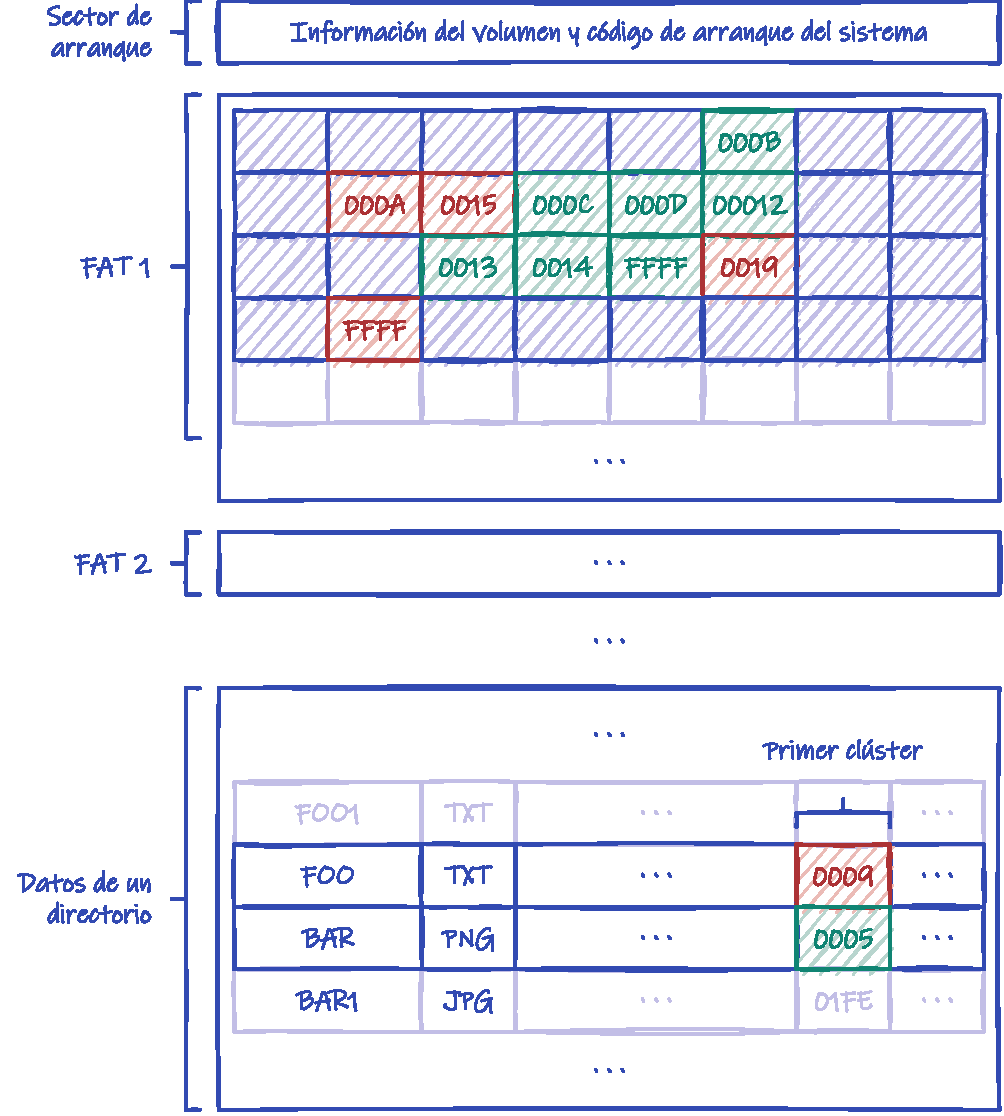
\includegraphics[width=0.8\textwidth]{media/C20_implemantación_sistema_de_archivos/estructura_fat.pdf}
\caption{Asignación enlazada en el sistema de archivos
FAT.}\label{fig-estructura-fat}
\end{figure}

Una de las ventajas de este esquema es que mejora el tiempo de los
accesos aleatorios a los archivos ---respecto a la asignación enlazada
convencional--- porque se puede conocer la ubicación de cualquier bloque
a partir de la información en la FAT, sin tener que leer todos los
bloques del archivo uno a uno.

\subsection{Asignación indexada}\label{_asignaciuxf3n_indexada}

{} El mecanismo de \textbf{asignación indexada} agrupa todos los
punteros de la asignación enlazada en una única ubicación: el
\textbf{bloque de índices}{}. Así se resuelve la falta de eficiencia de
la asignación enlazada convencional ---en ausencia de FAT--- cuando se
realizan accesos aleatorios.

En la \textbf{asignación indexada}:

\begin{itemize}
\item
  Cada archivo tiene su propio \textbf{bloque de índices}, que es un
  bloque del disco con una tabla con los números de los bloques del
  disco que contienen los datos del archivo.
\item
  La entrada i-ésima del bloque de índice contiene la dirección del
  bloque i-ésimo del archivo.
\item
  Cada entrada de directorio contiene la dirección del bloque de índices
  del archivo correspondiente.
\end{itemize}

Este mecanismo soporta el acceso aleatorio eficiente, además de no
sufrir el problema de la fragmentación externa. Sin embargo, también
tiene sus desventajas:

\begin{itemize}
\item
  Se pierde más espacio en los punteros que con el mecanismo de
  asignación enlazada, pues siempre hay que reservar un \textbf{bloque
  de índices} completo para cada archivo. Mientras que con la asignación
  enlazada, solo se pierde el espacio de los punteros que realmente es
  necesario utilizar.
\item
  Al diseñar el sistema de archivos debemos determinar el tamaño del
  \textbf{bloque de índices}.

  Por el inconveniente anterior y puesto que cada archivo debe tener un
  bloque de índices, ese bloque debe ser lo más pequeño posible para no
  perder espacio. Pero si es demasiado pequeño, no podrá almacenar
  suficientes punteros para un archivo de gran tamaño.
\end{itemize}

Entre los mecanismos que pueden utilizarse para resolver este último
problema están los siguientes:

\begin{itemize}
\item
  En el \textbf{esquema enlazado}{}, se enlazan los bloques de índices.

  Por ejemplo, se puede utilizar el último puntero del bloque de índices
  para apuntar al siguiente bloque de índices. Si dicho puntero tiene
  valor 0, entonces estamos en el último bloque de índices del archivo.
\item
  En el \textbf{índice multinivel}{}, los punteros del bloque de índices
  no señalan a los bloques del archivo, sino a un conjunto de bloques de
  índices de segundo nivel y estos, a su vez señalan, a los bloques del
  archivo. Esta técnica puede ampliarse utilizando un tercer o cuarto
  nivel, dependiendo del tamaño máximo de archivo que se desee.
\item
  En el \textbf{esquema combinado}{} las primeras entradas del bloque de
  índices apuntan directamente a los primeros bloques del archivo.
  Mientras que las siguientes entradas contiene punteros indirectos, que
  apunta a un conjunto de bloques de índices de segundo nivel. Después
  podría haber entradas que contienen punteros doblemente indirectos y
  luego entradas con punteros triplemente indirectos.
\end{itemize}

Para mejorar el rendimiento de los mecanismos de asignación indexados,
es muy común que el sistema operativo intente mantener los bloques de
índices en la memoria.

\begin{figure}
\centering
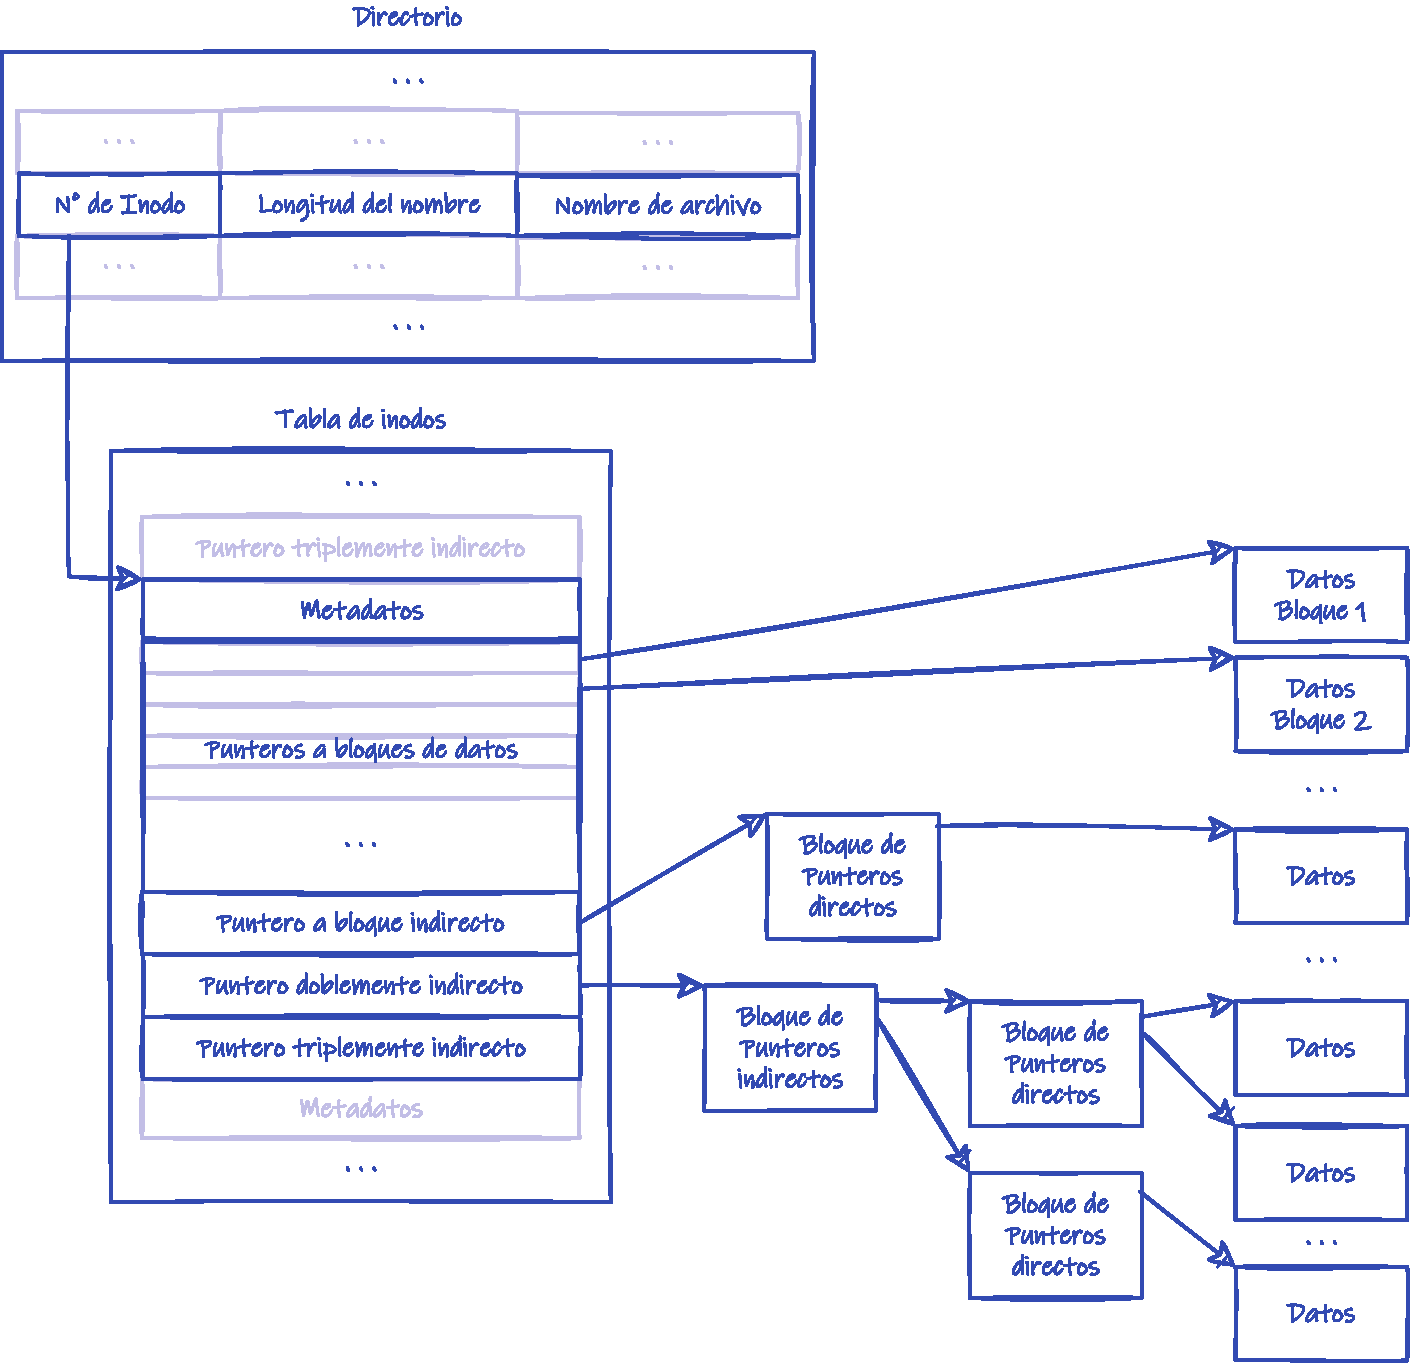
\includegraphics[width=0.8\textwidth]{media/C20_implemantación_sistema_de_archivos/asignación_ext2.pdf}
\caption{Asignación indexada combinada en el sistema de archivos
ext2.}\label{fig-asignaciuxf3n-ext2}
\end{figure}

Los sistemas de archivos \{ext2\} y \{ext3\} utilizan el mecanismo de
\textbf{asignación indexada} con \textbf{esquema combinado}.
Concretamente el mecanismo en \{ext2\} se implementa de la siguiente
manera:

\begin{itemize}
\item
  El disco se divide en múltiples grupos de bloques de disco.
\item
  En cada grupo, se utilizan los primeros bloques para almacenar una
  tabla de \textbf{inodos}{}. Estos \textbf{inodos} son los \textbf{FCB}
  de los archivos almacenados en el grupo.

  El resto de los bloques se utilizan para almacenar los datos de los
  archivos representados por los \textbf{inodos} del grupo.
\item
  Dentro de cada \textbf{inodo} ---entre otra información típica en un
  \textbf{FCB}--- se almacenan los punteros a los bloques del archivo,
  en lugar de utilizar un bloque de índices aparte.
\item
  Como se puede ver en la \hyperref[fig-asignaciuxf3n-ext2]{Asignación
  indexada combinada en el sistema de archivos ext2.}, los primeros 12
  punteros en el \textbf{inodo} son directos, seguidos de un puntero
  indirecto, un puntero doblemente indirecto y uno triplemente
  indirecto. Esto permite almacenar hasta 2\textsuperscript{64} bytes de
  información en cada archivo.
\end{itemize}

\section{Gestión del espacio libre}\label{_gestiuxf3n_del_espacio_libre}

Puesto que el espacio en disco es limitado, necesitamos poder reutilizar
el espacio de los archivos borrados. Para controlar el espacio libre en
el disco, el sistema de archivos mantiene una \textbf{lista de espacio
libre} que contiene todos los bloques de disco disponibles. Para crear
un archivo, se explora la \textbf{lista de espacio libre} hasta obtener
la cantidad de espacio requerida y se asigna ese espacio al nuevo
archivo.

A continuación estudiaremos las diferentes maneras de implementar esa
lista.

\subsection{Vector de bits}\label{_vector_de_bits}

La lista de espacio libre puede ser implementada como un \textbf{vector
de bits} o \textbf{mapa de bits}, donde cada bloque es representado por
un bit. Si el bloque está libre, el bit está a 1, mientras que si el
bloque está asignado, el bit está a 0.

Este enfoque es relativamente sencillo y eficiente, puesto que muchos
procesadores disponen de instrucciones para manipular bits, que pueden
utilizarse para obtener rápidamente el primer bloque libre. Por ejemplo,
la familia de procesadores \{x86\}, a partir del \{intel80386\}, tiene
instrucciones que devuelven la posición del primer bit a 1 en el valor
de un registro.

Sin embargo, leer el vector de bits, modificarlo y actualizarlo en disco
en cada ocasión, es tremendamente ineficiente. Por tanto, usar vectores
de bits es ineficiente, a menos que se mantenga el vector completo en la
memoria principal, escribiéndose ocasionalmente en el disco.

Esto último puede ser imposible para los discos de gran tamaño, en
función de la cantidad de memoria principal. Por ejemplo, un disco de 40
GiB con bloques de 512 bytes necesitará un mapa de bits de más de 10
MiB, lo que no es un gran requisito para un sistema moderno, pero sí lo
era hace dos décadas.

El sistema de archivo NTFS y la familia \emph{extended filesystem} ---es
decir, \{ext\}, \{ext2\}, \{ext3\} y \{ext4--- utilizan mapas de bits,
tanto para gestionar los bloques de datos libres como las entradas
disponibles en la tabla de \textbf{inodos}.

\subsection{Lista enlazada}\label{_lista_enlazada}

Otra técnica consiste en enlazar todos los bloques de disco libres. Para
eso se puede guardar un puntero al primer bloque libre en una ubicación
especial del disco y que ese bloque contenga un puntero al siguiente
bloque libre del disco. El segundo bloque contenga un puntero al tercer
bloque libre, y así sucesivamente.

El inconveniente es que recorrer la lista no resulta eficiente, pues
tenemos que leer cada bloque para conocer la dirección del siguiente
bloque libre en disco. Sin embargo, debemos tener en cuenta que no es
frecuente tener que recorrer la lista de espacio libre completa porque,
por lo general, basta con encontrar el primer bloque libre para asignar
el espacio.

Los sistemas de archivos \{fat\} incorporan el control de bloques libres
dentro de la \textbf{tabla de asignación de archivos} guardando un 0 en
las entradas de los \textbf{clústeres} libres, por lo que no se necesita
ningún método adicional.

\subsection{Agrupamiento}\label{_agrupamiento}

Una modificación de la técnica basada en la lista enlazada consiste en
almacenar las direcciones de \emph{N} bloques libres en el primer bloque
libre. Los primeros \emph{N --- 1} de esos bloques estarían realmente
libres, pero el último de ellos apuntaría a otro bloque con \emph{N}
bloques libres. Así podrían localizarse rápidamente las direcciones de
un gran número de bloques libres, lo cual mejora la eficiencia respecto
a la técnica de lista enlazada.

\subsection{Recuento}\label{_recuento}

Generalmente los bloques son asignados o liberados en bloques contiguos,
especialmente si el espacio es asignado mediante asignación contigua o
en \textbf{extensiones} o \textbf{clústeres}. Esto puede ser aprovechado
para mantener una lista donde cada entrada almacena la dirección del
primer bloque de un conjunto de bloques libres contiguo, así como el
número de bloques del conjunto.

Por ejemplo, el sistema de archivos \{xfs\} utiliza un árbol B+ para
almacenar las direcciones de las extensiones de bloques libres y
mantenerlas ordenadas por el tamaño de la extensión a la que apuntan.
Así el sistema operativo puede localizar rápidamente el espacio libre
necesario para satisfacer una necesidad concreta.

\section{Sistemas de archivos
virtuales}\label{_sistemas_de_archivos_virtuales}

En el \hyperref[_montaje_de_sistemas_de_archivos]{???} vimos cómo el
sistema operativo \textbf{monta} sistemas de archivos de tal forma que
aparenten estar integrados en una única estructura de directorios,
permitiendo a los usuarios moverse de forma transparente entre distintos
dispositivos y tipos de sistemas de archivos. Para hacerlo, un sistema
operativo moderno debe ser capaz de soportar de manera eficiente
distintos tipos de sistemas de archivos, ocultando sus diferencias de
cara a los usuarios.

Un método para implementar múltiples tipos de sistemas de archivos
consiste en escribir diferentes rutinas de acceso, manipulación y
gestión ---de los directorios y archivos--- para cada uno de los tipos
de sistema de archivo existentes. Sin embargo, en lugar de esta
solución, la mayoría de los sistemas operativos utilizan técnicas de
programación orientada a objetos para implementar diferentes tipos de
sistemas de archivos detrás de una misma interfaz de programación. Es
decir, se utilizan estructuras de datos y procedimientos comunes para
separar las llamadas al sistema de los detalles de su implementación
real, para cada uno de los sistemas de archivos.

La implementación de un sistema de archivos está compuesta de tres
niveles fundamentales: la \textbf{interfaz del sistema de archivos}, el
\textbf{sistema de archivos virtual} y, finalmente, la implementación
real del sistema de archivos.

\subsection{Interfaz del sistema de
archivos}\label{_interfaz_del_sistema_de_archivos}

{} El primer nivel es la \textbf{interfaz del sistema de archivos}, a la
que acceden los desarrolladores a través de las llamadas al sistema. En
sistemas POSIX, estamos hablando de las llamadas \{linux\_open\},
\{linux\_read\}, \{linux\_write\} y \{linux\_close\}, entre otras. Y de
los descriptores de archivos con los que se identifican los archivos
abiertos.

Esta interfaz es la misma sea cual sea el sistema de archivos al que se
esté intentando acceder.

\subsection{Sistema de archivos
virtual}\label{_sistema_de_archivos_virtual}

{} El segundo nivel es la interfaz del \textbf{sistema de archivos
virtual} o \textbf{{}VFS} (\emph{Virtual File System}). Este nivel es
utilizado por el anterior para atender las peticiones realizadas.

Describe operaciones genéricas sobre cualquier sistema de archivos y
estructuras genéricas. Por ejemplo, el \textbf{FCB virtual}{}, que
identifica de forma unívoca a cada archivo o directorio en uso en todo
el sistema, dando acceso a sus metadatos.

En Linux el \textbf{FCB virtual} se denomina \textbf{{}vnodo}. El
\textbf{vnodo} de un archivo lo identifica de forma unívoca en todo el
sistema, incluso diferenciando archivos en sistemas de archivos
diferentes. Mientras que el \textbf{inodo} es un detalle de la
implementación real del sistema de archivos, por lo que solo es único
dentro del mismo sistema de archivos.

Este nivel cumple con dos importantes funciones:

\begin{itemize}
\item
  Separa las operaciones genéricas sobre el sistema de archivos con
  respecto a su implementación.

  \textbf{VFS} define una interfaz muy clara y común para todos los
  sistemas de archivos. De esta interfaz existirán diversas
  implementaciones en el mismo sistema, una para cada sistema de
  archivos diferente.
\item
  Proporcionar un mecanismo para acceder de forma coherente a los
  archivos a través de la red.

  Una implementación de \textbf{VFS} no tiene que estar limitada
  exclusivamente a ofrecer acceso a archivos en dispositivos conectados
  físicamente al sistema. Las operaciones de la interfaz \textbf{VFS}
  pueden implementarse de tal forma que usen un protocolo de acceso a
  algún servidor de archivos conectado a la red.
\end{itemize}

\subsection{Implementación del sistema de
archivos}\label{_implementaciuxf3n_del_sistema_de_archivos}

El tercer nivel es donde se implementa cada tipo de sistema de archivos
o los distintos protocolos de los servidores de archivos en la red. La
interfaz \textbf{VFS} recurre a la implementación correspondiente para
cada tipo de sistema de archivos, para satisfacer las solicitudes de los
niveles superiores.

Así, por ejemplo, un \{linux\_read\} puede implicar que se tenga que
recuperar el \textbf{vnodo} del archivo involucrado desde la tabla de
archivos abiertos, usando el descriptor de archivo indicado en la
llamada al sistema. Después, se invoca la operación \textbf{VFS}
\texttt{read()} sobre el \textbf{vnodo}, en la implementación concreta
de \textbf{VFS} según el tipo de sistema de archivos involucrado. Será
esa implementación quien extraiga del \textbf{vnodo} la información
necesaria ---por ejemplo, el \textbf{inodo} real del archivo en el
sistema de archivos--- para llevar a cabo la operación indicada, según
las especificidades del sistema de archivos.

\section{Planificación de disco}\label{_planificaciuxf3n_de_disco}

Como ya hemos comentado, es responsabilidad del sistema operativo usar
los recursos del hardware de forma eficiente. Eso incluye planificar los
procesos en la CPU para conseguir el mínimo tiempo de espera que sea
posible o aprovechar de la mejor forma la memoria principal disponible
para atender la demanda de los distintos procesos al mismo tiempo; pero
también, intentar obtener el menor tiempo de acceso y el mayor ancho de
banda posible en el acceso a los discos.

\subsection{Rendimiento del acceso a
disco}\label{_rendimiento_del_acceso_a_disco}

En un disco duro magnético el \textbf{tiempo de acceso al disco}{}
\emph{T\textsuperscript{d}} viene determinado por el \textbf{tiempo de
búsqueda} \emph{T\textsuperscript{b}} y la \textbf{latencia rotacional}
\emph{T\textsuperscript{r}}:

\[T_d=T_b+T_r\]

El \textbf{tiempo de búsqueda}{} \emph{T\textsuperscript{b}} es el
tiempo que se tarda en mover el brazo del disco hasta el cilindro
deseado. Mientras que la \textbf{latencia rotacional}{}
\emph{T\textsuperscript{r}} es el tiempo que hay que esperar para que el
disco gira hasta que la cabeza llegue al sector deseado del cilindro.
Por lo tanto, el \textbf{tiempo de acceso al disco} es menor cuando se
realizan accesos consecutivos a sectores físicamente próximos que cuando
están dispersos por todo el disco.

El \textbf{{}ancho de banda} o \textbf{tasa de transferencia}{} del
disco es el total de bytes transferidos en una petición dividida por el
tiempo total que transcurre desde la primera solicitud de servicio hasta
el final de la última transferencia, con la que se termina de atender la
petición. Al considerar todo el tiempo necesario para atender la
petición, a más \textbf{tiempo de acceso al disco} menor es el
\textbf{ancho de banda}.

En los dispositivos de almacenamiento basados en memorias de estado
sólido (véase el \hyperref[_memorias_de_estado_suxf3lido]{???}) el
tiempo de acceso viene determinado por las características de la memoria
---entre otros factores--- lo que hace que las diferencias entre accesos
secuenciales y accesos aleatorios sean mucho menos significativas.

\subsection{Cola de E/S al disco}\label{_cola_de_es_al_disco}

{} Cuando se solicita una operación de E/S sobre el almacenamiento, si
la controladora y la unidad de disco están desocupadas, el sistema
operativo puede atender la petición sobre la marcha. Pero si están
ocupadas, el sistema operativo almacena la solicitud en una cola de
peticiones pendientes. Cuando se resuelve una solicitud, el sistema
operativo escoge otra de la cola y se comunica con el hardware para
programar la siguiente petición. La cuestión es ¿cuál es el orden
adecuado para escoger la peticiones de E/S de la cola, si se quiere
acceder al disco de la forma más eficaz posible?

\subsection{Planificación FCFS}\label{_planificaciuxf3n_fcfs}

{} En la planificación \textbf{{}FCFS} (\emph{First Come, First Served})
o \textbf{primero que llega, primero servido} la cola de E/S al disco es
FIFO. Es decir, que las solicitudes se atienden en orden de llegada.

Es el algoritmo de planificación más simple y es equitativo, en sentido
de que atiende a todos los procesos por igual. Pero, lamentablemente, no
proporciona el servicio más rápido en discos duros magnéticos, donde
interesa mover el brazo del disco lo menos posible.

En Linux el \textbf{FCFS} es actualmente denominado \textbf{NOOP}. Se
suele utilizar en los discos basados en memorias de estado sólido, donde
reordenar las solicitudes no proporciona una mejora significativa del
rendimiento, o cuando se utilizan controladoras de disco inteligentes
que pueden reordenar las solicitudes según su propio criterio.

\subsection{Planificación SSTF}\label{_planificaciuxf3n_sstf}

{} En la planificación \textbf{{}SSTF} (\emph{Sortest} \emph{Seek Time
First}) o algoritmo de \textbf{tiempo de búsqueda más corto}, de toda
cola se selecciona la solicitud con el menor \textbf{tiempo de búsqueda}
desde la posición actual de la cabeza. Este algoritmo de planificación
primero da servicio a las solicitudes cercanas a la posición actual de
la cabeza, antes de alejarse para dar servicio a otras solicitudes, dado
que el \textbf{tiempo de búsqueda} se incrementa a medida que lo hace el
número de cilindros que es necesario recorrer para llegar a una posición
dada.

Aun así, la solución no es óptima, dado que puede provocar inanición de
algunas solicitudes, si van llegando constantemente nuevas solicitudes
sobre regiones cercanas a donde está actualmente la cabeza del disco.

\subsection{Planificación SCAN y
C-SCAN}\label{_planificaciuxf3n_scan_y_c_scan}

{} {} En la planificación \textbf{{}SCAN}, algoritmo de
\textbf{exploración} o del \textbf{ascensor}, el brazo del disco
comienza en un extremo del disco y se mueve hacia el otro, atendiendo
solicitudes a medida que pasa por cada cilindro, hasta llegar al otro
extremo del disco. En el otro extremo, la dirección de movimiento de la
cabeza se invierte para recorrer el disco en sentido inverso, repitiendo
el proceso.

Suponiendo que las solicitudes se distribuyen de forma uniforme a lo
largo del disco, es de suponer que cuando se llega a un extremo ---justo
antes de volver--- la cantidad de solicitudes en dicho extremo será
notablemente menor que dónde comenzó el barrido que acaba de terminar.
Entonces ¿por qué no volver a empezar desde ese extremo?

A la variante del \textbf{SCAN} que cuando llega a un extremo vuelve al
inicio, para volver a barrer desde allí, sin atender ninguna solicitud
por el camino, se la denomina \textbf{{}C-SCAN} ---de \emph{Circula
SCAN}---. Con esta variante el tiempo que tiene que esperar una
solicitud para ser atendida es más uniforme que con el algoritmo
\textbf{SCAN} original.

\subsection{Planificación LOOK y
C-LOOK}\label{_planificaciuxf3n_look_y_c_look}

{} {} En teoría los algoritmos \textbf{SCAN} y \textbf{C-SCAN} hacen que
el brazo recorra los cilindros del primero al último, pero normalmente
no se suelen implementar así.

Por lo general, cuando en el recorrido del brazo, tras atender una
solicitud, se descubre que ya no hay más solicitudes siguiendo la misma
dirección, el brazo invierte la dirección sin llegar hasta el extremo
del disco.

A estas variantes de \textbf{SCAN} y \textbf{C-SCAN} se las denomina
\textbf{(LOOK)} y \textbf{(C-LOOK)}, respectivamente.

Linux utilizó \textbf{C-LOOK}, bajo el nombre de
\textbf{\emph{elevator}}, como planificador de E/S de disco hasta Linux
2.6.

\subsection{Planificación N-Step-SCAN, N-Step-LOOK y
F-SCAN}\label{_planificaciuxf3n_n_step_scan_n_step_look_y_f_scan}

{} {} {} Los algoritmos \textbf{{}N-Step-SCAN} y \textbf{{}N-Step-LOOK}
son variantes de los algoritmos \textbf{SCAN} y \textbf{LOOK},
respectivamente; donde se limita a \emph{N} el número de solicitudes que
se atenderán en cada barrido del brazo del disco. Estos algoritmos
funcionan de la siguiente manera:

\begin{enumerate}
\def\labelenumi{\arabic{enumi}.}
\item
  Se utiliza una cola con espacio para \emph{N} solicitudes pendientes,
  que se van atendiendo mientras el brazo barre el disco.
\item
  Mientras tanto, todas las nuevas solicitudes se incorporan a una cola
  diferente.
\item
  Cuando el brazo termina el barrido y las \emph{N} primeras solicitudes
  han sido atendidas, el planificador toma otras \emph{N} solicitudes de
  la segunda cola y las introduce en la primera para repetir el proceso.
\end{enumerate}

Si en lugar de copiar \emph{N} peticiones de la segunda a la primera
cola, se copian todas las solicitudes pendientes, el algoritmo se
denomina \textbf{{}F-SCAN}.

Estos algoritmos previenen un problema denominado \textbf{{}rigidez del
brazo} ---o \emph{arm stickiness}, en inglés--- a diferencia de los
algoritmos SSTF, SCAN, C-SCAN, LOOK y C-LOOK, que no lo hacen. El
término \textbf{rigidez del brazo} hace referencia a cuando hay un flujo
continuo de solicitudes para el mismo cilindro, esto hace que con los
algoritmos vistos hasta ahora, el brazo no avance por los cilindros
hasta llegar al otro extremo. Como \textbf{F-SCAN}, \textbf{N-Step-SCAN}
y \textbf{N-Step-LOOK} separan las solicitudes en dos colas ---haciendo
que las nuevas tengan que esperar--- el brazo siempre continúa su
barrido hacia el extremo del disco.

\subsection{Planificación CFQ}\label{_planificaciuxf3n_cfq}

{} El planificador \textbf{{}CFQ} (\emph{Completely Fair Queuing}) se
diseñó para compartir de forma equitativa el \textbf{ancho de banda}
entre todos los procesos que solicitan acceso al disco. Fue utilizado
por defecto en muchas distribuciones de Linux hasta la versión 5.0 del
núcleo y funciona de la siguiente manera:

\begin{itemize}
\item
  \textbf{CFQ} mantiene una cola de solicitudes para cada proceso y en
  ella inserta las solicitudes síncronas de E/S. Cada cola tiene una
  ventana de tiempo ---o \textbf{cuanto}--- para acceder al disco. La
  longitud del \textbf{cuanto} y el tamaño máximo de cada cola dependen
  de la prioridad de E/S que tenga el proceso.
\end{itemize}

Las solicitudes síncronas de E/S son aquellas que hacen que el proceso
permanezca en estado \textbf{esperando} hasta que se resuelve la
petición. Por ejemplo, las operaciones de lectura bloqueantes, como
ocurre por defecto con \{linux\_read\}. Mientras que las solicitudes
asíncronas son las que permiten que el proceso continúe su ejecución en
la CPU mientras se atiende la petición. Como las escrituras con
\{linux\_write\}.

\begin{itemize}
\item
  \textbf{CFQ} mantiene una cola de solicitudes por cada prioridad de
  E/S, donde se insertan las solicitudes asíncronas de todos los
  procesos. Una solicitud asíncrona se inserta en una cola u otra según
  la prioridad del proceso que la generó.
\item
  Usando el algoritmo \textbf{\emph{round-robin}}, el planificador
  \textbf{CFQ} recorre las colas y extrae de ellas las solicitudes
  durante el tiempo marcado por el cuanto de cada cola. Las solicitudes
  extraídas se insertan en la cola de E/S al disco, donde se ordenan
  para minimizar el \textbf{tiempo de búsqueda}, antes de ser enviadas
  al dispositivo.
\end{itemize}

Actualmente, los planificadores \textbf{CFS} y \textbf{NOOP} se
consideran obsoletos. En su lugar el planificador por defecto en Linux
para SSD y discos duros es \textbf{mq-deadline} ---una adaptación del
planificador
\href{https://en.wikipedia.org/wiki/Deadline_scheduler}{deadline},
también obsoleto---. Mientras que para dispositivos NVM Express se
utiliza \textbf{NONE}, que básicamente desactiva la planificación de la
E/S de disco.

Otros planificadores disponibles actualmente son
\href{https://algo.ing.unimo.it/people/paolo/disk_sched/}{BFQ}
---diseñado para minimizar la latencia--- y Kyber.


\backmatter
\printindex

\end{document}
